\documentclass[12pt,a4paper]{article}

\textwidth16.5cm
\textheight23cm
\oddsidemargin0cm
\evensidemargin0cm
\topmargin-2cm
\usepackage{xspace}
\usepackage[normalem]{ulem}
\usepackage{cite}
\usepackage{multirow}
\usepackage[breaklinks,hidelinks]{hyperref}
\usepackage{graphicx}
\graphicspath{{figures/generated/}{figures/legacy/}{figures/}}
\usepackage[labelfont=bf,font=small,skip=0pt]{caption}
\usepackage{subcaption}
%\usepackage[demo]{graphicx}
%\usepackage{subcaption}
%\usepackage{subfig}
\usepackage{amscd}
\usepackage{mathrsfs}
\usepackage{longtable}
\usepackage{booktabs}
\usepackage{array}
\usepackage{epstopdf}
\usepackage{xcolor}
\usepackage{soul,xcolor}
\usepackage{float}
\usepackage{url}
\usepackage{latexsym}
\usepackage{amsthm}
\usepackage{mathtools}
\usepackage{amssymb}
\usepackage{tikz}
\usepackage{pgfplots}
\pgfplotsset{compat=1.18}
\usetikzlibrary{positioning,arrows.meta,shapes.geometric,calc,fit,backgrounds,decorations.pathreplacing}
\usepackage{algorithm}
\usepackage{algpseudocode}
\usepackage{siunitx}
\usepackage{amsmath}
\usepackage{bm}

% ------------------------------------------------------------
% Acronyms: use only the shortcut commands below in the paper
% ------------------------------------------------------------
\usepackage{acro}

\DeclareAcronym{cfd}{
  short = CFD,
  long  = computational fluid dynamics
}

\DeclareAcronym{fsi}{
  short = FSI,
  long  = fluid--structure interaction
}

\DeclareAcronym{pinn}{
  short = PINN,
  long  = physics-informed neural network
}

\DeclareAcronym{dtaa}{
  short = DTAA,
  long  = descending thoracic aortic aneurysm
}

\DeclareAcronym{wss}{
  short = WSS,
  long  = wall shear stress
}

\DeclareAcronym{wssg}{
  short = WSSG,
  long  = wall shear stress gradient
}

\DeclareAcronym{tawss}{
  short = TAWSS,
  long  = time-averaged wall shear stress
}

\DeclareAcronym{mps}{
  short = MPS,
  long  = maximum principal stress
}

\DeclareAcronym{tke}{
  short = TKE,
  long  = turbulent kinetic energy
}

\DeclareAcronym{rans}{
  short = RANS,
  long  = Reynolds-averaged Navier--Stokes
}

\DeclareAcronym{sst}{
  short = SST,
  long  = shear stress transport
}

\DeclareAcronym{gci}{
  short = GCI,
  long  = grid convergence index
}

\DeclareAcronym{aa}{
  short = AA,
  long  = aortic aneurysm
}

\DeclareAcronym{NRMSE}{
  short = NRMSE,
  long  = normalized root mean square error
}

\DeclareAcronym{OSI}{
  short = OSI,
  long  = oscillatory shear index
}

\DeclareAcronym{ICA}{
  short = ICA,
  long  = internal carotid artery
}

\DeclareAcronym{AR}{
  short = AR,
  long  = aspect ratio
}

\DeclareAcronym{SR}{
  short = SR,
  long  = size ratio
}

\DeclareAcronym{RRT}{
  short = RRT,
  long  = relative residence time
}

\DeclareAcronym{ECAP}{
  short = ECAP,
  long  = endothelial cell activation potential
}

\DeclareAcronym{DNS}{
  short = DNS,
  long  = direct numerical simulation
}

\DeclareAcronym{LDL}{
  short = LDL,
  long  = low-density lipoprotein
}

\DeclareAcronym{ICRZ}{
  short = ICRZ,
  long  = inner curvature recirculation zone
}

\DeclareAcronym{SD}{
  short = SD,
  long  = standard deviation
}

\DeclareAcronym{urans}{
  short = URANS,
  long  = unsteady Reynolds-averaged Navier--Stokes
}

% ------------------------------------------------------------
% Lowercase default shortcuts
% These give the lowercase long form on first use
% (e.g. “wall shear stress”) and the acronym later (e.g. “WSS”).
% ------------------------------------------------------------
\newcommand{\CFD}{\ac{cfd}\xspace}
\newcommand{\FSI}{\ac{fsi}\xspace}
\newcommand{\PINN}{\ac{pinn}\xspace}
\newcommand{\PINNs}{\acp{pinn}\xspace}
\newcommand{\DTAA}{\ac{dtaa}\xspace}
\newcommand{\DTAAs}{\acp{dtaa}\xspace}
\newcommand{\WSS}{\ac{wss}\xspace}
\newcommand{\WSSG}{\ac{wssg}\xspace}
\newcommand{\TAWSS}{\ac{tawss}\xspace}
\newcommand{\MPS}{\ac{mps}\xspace}
\newcommand{\TKE}{\ac{tke}\xspace}
\newcommand{\RANS}{\ac{rans}\xspace}
\newcommand{\SST}{\ac{sst}\xspace}
\newcommand{\GCI}{\ac{gci}\xspace}
\newcommand{\AAN}{\ac{aa}\xspace}
\newcommand{\AANs}{\acp{aa}\xspace}
\newcommand{\NRMSE}{\ac{NRMSE}\xspace}
\newcommand{\OSI}{\ac{OSI}\xspace}
\newcommand{\ICA}{\ac{ICA}\xspace}
\newcommand{\AR}{\ac{AR}\xspace}
\newcommand{\SR}{\ac{SR}\xspace}
\newcommand{\RRT}{\ac{RRT}\xspace}
\newcommand{\ECAP}{\ac{ECAP}\xspace}
\newcommand{\DNS}{\ac{DNS}\xspace}
\newcommand{\LDL}{\ac{LDL}\xspace}
\newcommand{\ICRZ}{\ac{ICRZ}\xspace}
\newcommand{\SD}{\ac{SD}\xspace}
\newcommand{\URANS}{\ac{urans}\xspace}

% ------------------------------------------------------------
% Uppercase variants for use at the start of a sentence,
% in a heading, etc.
% These give the capitalised long form on first use
% (e.g. “Wall shear stress”) and the acronym later (e.g. “WSS”).
% ------------------------------------------------------------
\newcommand{\CFDcap}{\Ac{cfd}\xspace}
\newcommand{\FSIcap}{\Ac{fsi}\xspace}
\newcommand{\PINNcap}{\Ac{pinn}\xspace}
\newcommand{\PINNscap}{\Acp{pinn}\xspace}
\newcommand{\DTAAcap}{\Ac{dtaa}\xspace}
\newcommand{\DTAAscap}{\Acp{dtaa}\xspace}
\newcommand{\WSScap}{\Ac{wss}\xspace}
\newcommand{\WSSGcap}{\Ac{wssg}\xspace}
\newcommand{\TAWSScap}{\Ac{tawss}\xspace}
\newcommand{\MPScap}{\Ac{mps}\xspace}
\newcommand{\TKEcap}{\Ac{tke}\xspace}
\newcommand{\RANScap}{\Ac{rans}\xspace}
\newcommand{\SSTcap}{\Ac{sst}\xspace}
\newcommand{\GCIcap}{\Ac{gci}\xspace}
\newcommand{\AANcap}{\Ac{aa}\xspace}
\newcommand{\AANscap}{\Acp{aa}\xspace}
\newcommand{\NRMSEcap}{\Ac{NRMSE}\xspace}
\newcommand{\OSIcap}{\Ac{OSI}\xspace}
\newcommand{\ICAcap}{\Ac{ICA}\xspace}
\newcommand{\ARcap}{\Ac{AR}\xspace}
\newcommand{\SRcap}{\Ac{SR}\xspace}
\newcommand{\RRTcap}{\Ac{RRT}\xspace}
\newcommand{\ECAPcap}{\Ac{ECAP}\xspace}
\newcommand{\DNScap}{\Ac{DNS}\xspace}
\newcommand{\LDLcap}{\Ac{LDL}\xspace}
\newcommand{\ICRZcap}{\Ac{ICRZ}\xspace}
\newcommand{\SDcap}{\Ac{SD}\xspace}
\newcommand{\URANScap}{\Ac{urans}\xspace}



\DeclareAcronym{rbf}{
  short = RBF,
  long  = radial basis function
}

% lowercase shortcut
\newcommand{\RBF}{\ac{rbf}\xspace}
% capitalised variant
\newcommand{\RBFcap}{\Ac{rbf}\xspace}
% Chinese glyphs for the co-author name; compiles under pdfLaTeX (CJKutf8) and
% XeLaTeX/LuaLaTeX (fontspec), so no compiler switch is needed on Overleaf.
\usepackage{iftex}
\ifPDFTeX
  \usepackage{CJKutf8}
  \newcommand{\cjkname}[1]{\begin{CJK}{UTF8}{gbsn}#1\end{CJK}}
\else
  \usepackage{fontspec}
  \newfontfamily\cjkfont{Noto Serif CJK SC}
  \newcommand{\cjkname}[1]{{\cjkfont #1}}
\fi

\newcommand{\R}{\mathbb{R}}
\renewcommand{\vec}[1]{\boldsymbol{\mathbf{#1}}}

\usepackage{setspace}

% Redefine the format of section numbering
\renewcommand\thesection{\textcolor{blue}{\arabic{section}}}

% Redefine the format of subsection numbering
\renewcommand\thesubsection{\thesection.\textcolor{blue}{\arabic{subsection}}}

% Set the paragraph indentation
\setlength{\parindent}{1cm}

% Absorb small over/underfull boxes
\setlength{\emergencystretch}{2em}

% Keep short floats with the text; use fixed gaps on dedicated float pages.
\renewcommand{\topfraction}{0.92}
\renewcommand{\bottomfraction}{0.9}
\renewcommand{\textfraction}{0.08}
\renewcommand{\floatpagefraction}{0.75}
\setcounter{topnumber}{4}
\setcounter{bottomnumber}{4}
\setcounter{totalnumber}{8}
\setlength{\textfloatsep}{12pt plus 2pt minus 2pt}
\setlength{\floatsep}{10pt plus 2pt minus 2pt}
\setlength{\intextsep}{10pt plus 2pt minus 2pt}
\makeatletter
\setlength{\@fptop}{0pt}
\setlength{\@fpsep}{12pt}
\setlength{\@fpbot}{0pt plus 1fil}
\makeatother
\raggedbottom

%\usepackage{eufrak}
%\def\principaladviser#1{\gdef\@principaladviser{#1}}

%\usepackage[all]{xy}
\usepackage{epsfig}

%\usepackage{apst-all}
%\usepackage{xy-pic}
\usepackage[T1]{fontenc}
%\usepackage{dsfont}\let\mathbb\mathds

%\usepackage{fancyhdr}
\usepackage[arrow,frame,matrix]{xy}
\renewcommand{\baselinestretch}{1}

%\theoremstyle{plain}
%\newtheorem{Thm}{Theorem}[section]
%\newtheorem{lem}[Thm]{Lemma}
%\newtheorem{pro}[Thm]{Proposition}
%\newtheorem{de}[Thm]{Definition}
%\newtheorem{re}[Thm]{Remark}
%\newtheorem{ex}[Thm]{Example}
%\newtheorem{cor}[Thm]{Corollary}

%%%%%%%%%%%%%%%%%%%%%%%%%%%%%%
\theoremstyle{definition}
\newtheorem{Thm}{Theorem}[section]
\newtheorem{lem}[Thm]{Lemma}
\newtheorem{pro}[Thm]{Proposition}
\newtheorem{de}[Thm]{Definition}
\newtheorem{re}[Thm]{Remark}
\newtheorem{ex}[Thm]{Example}
\newtheorem{cor}[Thm]{Corollary}
%%%%%%%%%%%%%%%%%%%%%%%%%%%%%%%%%

\newcommand{\BibUrl}{\url}
\def\be{\begin{equation}}
\def\ee{\end{equation}}
\def\bea{\begin{eqnarray}}
\def\eea{\end{eqnarray}}
\numberwithin{equation}{section}

\title{\textbf{}}
\usepackage[section]{placeins}
\pgfplotsset{every axis/.append style={scaled ticks=false, tick label style={/pgf/number format/fixed}}}

% Anonymized copy for double-anonymized review (no names, affiliations, emails, funding or contributions):
%   pdflatex -output-directory=build -jobname=main_anonymized "\def\anonymized{}\documentclass[12pt,a4paper]{article}

\textwidth16.5cm
\textheight23cm
\oddsidemargin0cm
\evensidemargin0cm
\topmargin-2cm
\usepackage{xspace}
\usepackage[normalem]{ulem}
\usepackage{cite}
\usepackage{multirow}
\usepackage[breaklinks,hidelinks]{hyperref}
\usepackage{graphicx}
\graphicspath{{figures/generated/}{figures/legacy/}{figures/}}
\usepackage[labelfont=bf,font=small,skip=0pt]{caption}
\usepackage{subcaption}
%\usepackage[demo]{graphicx}
%\usepackage{subcaption}
%\usepackage{subfig}
\usepackage{amscd}
\usepackage{mathrsfs}
\usepackage{longtable}
\usepackage{booktabs}
\usepackage{array}
\usepackage{epstopdf}
\usepackage{xcolor}
\usepackage{soul,xcolor}
\usepackage{float}
\usepackage{url}
\usepackage{latexsym}
\usepackage{amsthm}
\usepackage{mathtools}
\usepackage{amssymb}
\usepackage{tikz}
\usepackage{pgfplots}
\pgfplotsset{compat=1.18}
\usetikzlibrary{positioning,arrows.meta,shapes.geometric,calc,fit,backgrounds,decorations.pathreplacing}
\usepackage{algorithm}
\usepackage{algpseudocode}
\usepackage{siunitx}
\usepackage{amsmath}
\usepackage{bm}

% ------------------------------------------------------------
% Acronyms: use only the shortcut commands below in the paper
% ------------------------------------------------------------
\usepackage{acro}

\DeclareAcronym{cfd}{
  short = CFD,
  long  = computational fluid dynamics
}

\DeclareAcronym{fsi}{
  short = FSI,
  long  = fluid--structure interaction
}

\DeclareAcronym{pinn}{
  short = PINN,
  long  = physics-informed neural network
}

\DeclareAcronym{dtaa}{
  short = DTAA,
  long  = descending thoracic aortic aneurysm
}

\DeclareAcronym{wss}{
  short = WSS,
  long  = wall shear stress
}

\DeclareAcronym{wssg}{
  short = WSSG,
  long  = wall shear stress gradient
}

\DeclareAcronym{tawss}{
  short = TAWSS,
  long  = time-averaged wall shear stress
}

\DeclareAcronym{mps}{
  short = MPS,
  long  = maximum principal stress
}

\DeclareAcronym{tke}{
  short = TKE,
  long  = turbulent kinetic energy
}

\DeclareAcronym{rans}{
  short = RANS,
  long  = Reynolds-averaged Navier--Stokes
}

\DeclareAcronym{sst}{
  short = SST,
  long  = shear stress transport
}

\DeclareAcronym{gci}{
  short = GCI,
  long  = grid convergence index
}

\DeclareAcronym{aa}{
  short = AA,
  long  = aortic aneurysm
}

\DeclareAcronym{NRMSE}{
  short = NRMSE,
  long  = normalized root mean square error
}

\DeclareAcronym{OSI}{
  short = OSI,
  long  = oscillatory shear index
}

\DeclareAcronym{ICA}{
  short = ICA,
  long  = internal carotid artery
}

\DeclareAcronym{AR}{
  short = AR,
  long  = aspect ratio
}

\DeclareAcronym{SR}{
  short = SR,
  long  = size ratio
}

\DeclareAcronym{RRT}{
  short = RRT,
  long  = relative residence time
}

\DeclareAcronym{ECAP}{
  short = ECAP,
  long  = endothelial cell activation potential
}

\DeclareAcronym{DNS}{
  short = DNS,
  long  = direct numerical simulation
}

\DeclareAcronym{LDL}{
  short = LDL,
  long  = low-density lipoprotein
}

\DeclareAcronym{ICRZ}{
  short = ICRZ,
  long  = inner curvature recirculation zone
}

\DeclareAcronym{SD}{
  short = SD,
  long  = standard deviation
}

\DeclareAcronym{urans}{
  short = URANS,
  long  = unsteady Reynolds-averaged Navier--Stokes
}

% ------------------------------------------------------------
% Lowercase default shortcuts
% These give the lowercase long form on first use
% (e.g. “wall shear stress”) and the acronym later (e.g. “WSS”).
% ------------------------------------------------------------
\newcommand{\CFD}{\ac{cfd}\xspace}
\newcommand{\FSI}{\ac{fsi}\xspace}
\newcommand{\PINN}{\ac{pinn}\xspace}
\newcommand{\PINNs}{\acp{pinn}\xspace}
\newcommand{\DTAA}{\ac{dtaa}\xspace}
\newcommand{\DTAAs}{\acp{dtaa}\xspace}
\newcommand{\WSS}{\ac{wss}\xspace}
\newcommand{\WSSG}{\ac{wssg}\xspace}
\newcommand{\TAWSS}{\ac{tawss}\xspace}
\newcommand{\MPS}{\ac{mps}\xspace}
\newcommand{\TKE}{\ac{tke}\xspace}
\newcommand{\RANS}{\ac{rans}\xspace}
\newcommand{\SST}{\ac{sst}\xspace}
\newcommand{\GCI}{\ac{gci}\xspace}
\newcommand{\AAN}{\ac{aa}\xspace}
\newcommand{\AANs}{\acp{aa}\xspace}
\newcommand{\NRMSE}{\ac{NRMSE}\xspace}
\newcommand{\OSI}{\ac{OSI}\xspace}
\newcommand{\ICA}{\ac{ICA}\xspace}
\newcommand{\AR}{\ac{AR}\xspace}
\newcommand{\SR}{\ac{SR}\xspace}
\newcommand{\RRT}{\ac{RRT}\xspace}
\newcommand{\ECAP}{\ac{ECAP}\xspace}
\newcommand{\DNS}{\ac{DNS}\xspace}
\newcommand{\LDL}{\ac{LDL}\xspace}
\newcommand{\ICRZ}{\ac{ICRZ}\xspace}
\newcommand{\SD}{\ac{SD}\xspace}
\newcommand{\URANS}{\ac{urans}\xspace}

% ------------------------------------------------------------
% Uppercase variants for use at the start of a sentence,
% in a heading, etc.
% These give the capitalised long form on first use
% (e.g. “Wall shear stress”) and the acronym later (e.g. “WSS”).
% ------------------------------------------------------------
\newcommand{\CFDcap}{\Ac{cfd}\xspace}
\newcommand{\FSIcap}{\Ac{fsi}\xspace}
\newcommand{\PINNcap}{\Ac{pinn}\xspace}
\newcommand{\PINNscap}{\Acp{pinn}\xspace}
\newcommand{\DTAAcap}{\Ac{dtaa}\xspace}
\newcommand{\DTAAscap}{\Acp{dtaa}\xspace}
\newcommand{\WSScap}{\Ac{wss}\xspace}
\newcommand{\WSSGcap}{\Ac{wssg}\xspace}
\newcommand{\TAWSScap}{\Ac{tawss}\xspace}
\newcommand{\MPScap}{\Ac{mps}\xspace}
\newcommand{\TKEcap}{\Ac{tke}\xspace}
\newcommand{\RANScap}{\Ac{rans}\xspace}
\newcommand{\SSTcap}{\Ac{sst}\xspace}
\newcommand{\GCIcap}{\Ac{gci}\xspace}
\newcommand{\AANcap}{\Ac{aa}\xspace}
\newcommand{\AANscap}{\Acp{aa}\xspace}
\newcommand{\NRMSEcap}{\Ac{NRMSE}\xspace}
\newcommand{\OSIcap}{\Ac{OSI}\xspace}
\newcommand{\ICAcap}{\Ac{ICA}\xspace}
\newcommand{\ARcap}{\Ac{AR}\xspace}
\newcommand{\SRcap}{\Ac{SR}\xspace}
\newcommand{\RRTcap}{\Ac{RRT}\xspace}
\newcommand{\ECAPcap}{\Ac{ECAP}\xspace}
\newcommand{\DNScap}{\Ac{DNS}\xspace}
\newcommand{\LDLcap}{\Ac{LDL}\xspace}
\newcommand{\ICRZcap}{\Ac{ICRZ}\xspace}
\newcommand{\SDcap}{\Ac{SD}\xspace}
\newcommand{\URANScap}{\Ac{urans}\xspace}



\DeclareAcronym{rbf}{
  short = RBF,
  long  = radial basis function
}

% lowercase shortcut
\newcommand{\RBF}{\ac{rbf}\xspace}
% capitalised variant
\newcommand{\RBFcap}{\Ac{rbf}\xspace}
% Chinese glyphs for the co-author name; compiles under pdfLaTeX (CJKutf8) and
% XeLaTeX/LuaLaTeX (fontspec), so no compiler switch is needed on Overleaf.
\usepackage{iftex}
\ifPDFTeX
  \usepackage{CJKutf8}
  \newcommand{\cjkname}[1]{\begin{CJK}{UTF8}{gbsn}#1\end{CJK}}
\else
  \usepackage{fontspec}
  \newfontfamily\cjkfont{Noto Serif CJK SC}
  \newcommand{\cjkname}[1]{{\cjkfont #1}}
\fi

\newcommand{\R}{\mathbb{R}}
\renewcommand{\vec}[1]{\boldsymbol{\mathbf{#1}}}

\usepackage{setspace}

% Redefine the format of section numbering
\renewcommand\thesection{\textcolor{blue}{\arabic{section}}}

% Redefine the format of subsection numbering
\renewcommand\thesubsection{\thesection.\textcolor{blue}{\arabic{subsection}}}

% Set the paragraph indentation
\setlength{\parindent}{1cm}

% Absorb small over/underfull boxes
\setlength{\emergencystretch}{2em}

% Keep short floats with the text; use fixed gaps on dedicated float pages.
\renewcommand{\topfraction}{0.92}
\renewcommand{\bottomfraction}{0.9}
\renewcommand{\textfraction}{0.08}
\renewcommand{\floatpagefraction}{0.75}
\setcounter{topnumber}{4}
\setcounter{bottomnumber}{4}
\setcounter{totalnumber}{8}
\setlength{\textfloatsep}{12pt plus 2pt minus 2pt}
\setlength{\floatsep}{10pt plus 2pt minus 2pt}
\setlength{\intextsep}{10pt plus 2pt minus 2pt}
\makeatletter
\setlength{\@fptop}{0pt}
\setlength{\@fpsep}{12pt}
\setlength{\@fpbot}{0pt plus 1fil}
\makeatother
\raggedbottom

%\usepackage{eufrak}
%\def\principaladviser#1{\gdef\@principaladviser{#1}}

%\usepackage[all]{xy}
\usepackage{epsfig}

%\usepackage{apst-all}
%\usepackage{xy-pic}
\usepackage[T1]{fontenc}
%\usepackage{dsfont}\let\mathbb\mathds

%\usepackage{fancyhdr}
\usepackage[arrow,frame,matrix]{xy}
\renewcommand{\baselinestretch}{1}

%\theoremstyle{plain}
%\newtheorem{Thm}{Theorem}[section]
%\newtheorem{lem}[Thm]{Lemma}
%\newtheorem{pro}[Thm]{Proposition}
%\newtheorem{de}[Thm]{Definition}
%\newtheorem{re}[Thm]{Remark}
%\newtheorem{ex}[Thm]{Example}
%\newtheorem{cor}[Thm]{Corollary}

%%%%%%%%%%%%%%%%%%%%%%%%%%%%%%
\theoremstyle{definition}
\newtheorem{Thm}{Theorem}[section]
\newtheorem{lem}[Thm]{Lemma}
\newtheorem{pro}[Thm]{Proposition}
\newtheorem{de}[Thm]{Definition}
\newtheorem{re}[Thm]{Remark}
\newtheorem{ex}[Thm]{Example}
\newtheorem{cor}[Thm]{Corollary}
%%%%%%%%%%%%%%%%%%%%%%%%%%%%%%%%%

\newcommand{\BibUrl}{\url}
\def\be{\begin{equation}}
\def\ee{\end{equation}}
\def\bea{\begin{eqnarray}}
\def\eea{\end{eqnarray}}
\numberwithin{equation}{section}

\title{\textbf{}}
\usepackage[section]{placeins}
\pgfplotsset{every axis/.append style={scaled ticks=false, tick label style={/pgf/number format/fixed}}}

% Anonymized copy for double-anonymized review (no names, affiliations, emails, funding or contributions):
%   pdflatex -output-directory=build -jobname=main_anonymized "\def\anonymized{}\documentclass[12pt,a4paper]{article}

\textwidth16.5cm
\textheight23cm
\oddsidemargin0cm
\evensidemargin0cm
\topmargin-2cm
\usepackage{xspace}
\usepackage[normalem]{ulem}
\usepackage{cite}
\usepackage{multirow}
\usepackage[breaklinks,hidelinks]{hyperref}
\usepackage{graphicx}
\graphicspath{{figures/generated/}{figures/legacy/}{figures/}}
\usepackage[labelfont=bf,font=small,skip=0pt]{caption}
\usepackage{subcaption}
%\usepackage[demo]{graphicx}
%\usepackage{subcaption}
%\usepackage{subfig}
\usepackage{amscd}
\usepackage{mathrsfs}
\usepackage{longtable}
\usepackage{booktabs}
\usepackage{array}
\usepackage{epstopdf}
\usepackage{xcolor}
\usepackage{soul,xcolor}
\usepackage{float}
\usepackage{url}
\usepackage{latexsym}
\usepackage{amsthm}
\usepackage{mathtools}
\usepackage{amssymb}
\usepackage{tikz}
\usepackage{pgfplots}
\pgfplotsset{compat=1.18}
\usetikzlibrary{positioning,arrows.meta,shapes.geometric,calc,fit,backgrounds,decorations.pathreplacing}
\usepackage{algorithm}
\usepackage{algpseudocode}
\usepackage{siunitx}
\usepackage{amsmath}
\usepackage{bm}

% ------------------------------------------------------------
% Acronyms: use only the shortcut commands below in the paper
% ------------------------------------------------------------
\usepackage{acro}

\DeclareAcronym{cfd}{
  short = CFD,
  long  = computational fluid dynamics
}

\DeclareAcronym{fsi}{
  short = FSI,
  long  = fluid--structure interaction
}

\DeclareAcronym{pinn}{
  short = PINN,
  long  = physics-informed neural network
}

\DeclareAcronym{dtaa}{
  short = DTAA,
  long  = descending thoracic aortic aneurysm
}

\DeclareAcronym{wss}{
  short = WSS,
  long  = wall shear stress
}

\DeclareAcronym{wssg}{
  short = WSSG,
  long  = wall shear stress gradient
}

\DeclareAcronym{tawss}{
  short = TAWSS,
  long  = time-averaged wall shear stress
}

\DeclareAcronym{mps}{
  short = MPS,
  long  = maximum principal stress
}

\DeclareAcronym{tke}{
  short = TKE,
  long  = turbulent kinetic energy
}

\DeclareAcronym{rans}{
  short = RANS,
  long  = Reynolds-averaged Navier--Stokes
}

\DeclareAcronym{sst}{
  short = SST,
  long  = shear stress transport
}

\DeclareAcronym{gci}{
  short = GCI,
  long  = grid convergence index
}

\DeclareAcronym{aa}{
  short = AA,
  long  = aortic aneurysm
}

\DeclareAcronym{NRMSE}{
  short = NRMSE,
  long  = normalized root mean square error
}

\DeclareAcronym{OSI}{
  short = OSI,
  long  = oscillatory shear index
}

\DeclareAcronym{ICA}{
  short = ICA,
  long  = internal carotid artery
}

\DeclareAcronym{AR}{
  short = AR,
  long  = aspect ratio
}

\DeclareAcronym{SR}{
  short = SR,
  long  = size ratio
}

\DeclareAcronym{RRT}{
  short = RRT,
  long  = relative residence time
}

\DeclareAcronym{ECAP}{
  short = ECAP,
  long  = endothelial cell activation potential
}

\DeclareAcronym{DNS}{
  short = DNS,
  long  = direct numerical simulation
}

\DeclareAcronym{LDL}{
  short = LDL,
  long  = low-density lipoprotein
}

\DeclareAcronym{ICRZ}{
  short = ICRZ,
  long  = inner curvature recirculation zone
}

\DeclareAcronym{SD}{
  short = SD,
  long  = standard deviation
}

\DeclareAcronym{urans}{
  short = URANS,
  long  = unsteady Reynolds-averaged Navier--Stokes
}

% ------------------------------------------------------------
% Lowercase default shortcuts
% These give the lowercase long form on first use
% (e.g. “wall shear stress”) and the acronym later (e.g. “WSS”).
% ------------------------------------------------------------
\newcommand{\CFD}{\ac{cfd}\xspace}
\newcommand{\FSI}{\ac{fsi}\xspace}
\newcommand{\PINN}{\ac{pinn}\xspace}
\newcommand{\PINNs}{\acp{pinn}\xspace}
\newcommand{\DTAA}{\ac{dtaa}\xspace}
\newcommand{\DTAAs}{\acp{dtaa}\xspace}
\newcommand{\WSS}{\ac{wss}\xspace}
\newcommand{\WSSG}{\ac{wssg}\xspace}
\newcommand{\TAWSS}{\ac{tawss}\xspace}
\newcommand{\MPS}{\ac{mps}\xspace}
\newcommand{\TKE}{\ac{tke}\xspace}
\newcommand{\RANS}{\ac{rans}\xspace}
\newcommand{\SST}{\ac{sst}\xspace}
\newcommand{\GCI}{\ac{gci}\xspace}
\newcommand{\AAN}{\ac{aa}\xspace}
\newcommand{\AANs}{\acp{aa}\xspace}
\newcommand{\NRMSE}{\ac{NRMSE}\xspace}
\newcommand{\OSI}{\ac{OSI}\xspace}
\newcommand{\ICA}{\ac{ICA}\xspace}
\newcommand{\AR}{\ac{AR}\xspace}
\newcommand{\SR}{\ac{SR}\xspace}
\newcommand{\RRT}{\ac{RRT}\xspace}
\newcommand{\ECAP}{\ac{ECAP}\xspace}
\newcommand{\DNS}{\ac{DNS}\xspace}
\newcommand{\LDL}{\ac{LDL}\xspace}
\newcommand{\ICRZ}{\ac{ICRZ}\xspace}
\newcommand{\SD}{\ac{SD}\xspace}
\newcommand{\URANS}{\ac{urans}\xspace}

% ------------------------------------------------------------
% Uppercase variants for use at the start of a sentence,
% in a heading, etc.
% These give the capitalised long form on first use
% (e.g. “Wall shear stress”) and the acronym later (e.g. “WSS”).
% ------------------------------------------------------------
\newcommand{\CFDcap}{\Ac{cfd}\xspace}
\newcommand{\FSIcap}{\Ac{fsi}\xspace}
\newcommand{\PINNcap}{\Ac{pinn}\xspace}
\newcommand{\PINNscap}{\Acp{pinn}\xspace}
\newcommand{\DTAAcap}{\Ac{dtaa}\xspace}
\newcommand{\DTAAscap}{\Acp{dtaa}\xspace}
\newcommand{\WSScap}{\Ac{wss}\xspace}
\newcommand{\WSSGcap}{\Ac{wssg}\xspace}
\newcommand{\TAWSScap}{\Ac{tawss}\xspace}
\newcommand{\MPScap}{\Ac{mps}\xspace}
\newcommand{\TKEcap}{\Ac{tke}\xspace}
\newcommand{\RANScap}{\Ac{rans}\xspace}
\newcommand{\SSTcap}{\Ac{sst}\xspace}
\newcommand{\GCIcap}{\Ac{gci}\xspace}
\newcommand{\AANcap}{\Ac{aa}\xspace}
\newcommand{\AANscap}{\Acp{aa}\xspace}
\newcommand{\NRMSEcap}{\Ac{NRMSE}\xspace}
\newcommand{\OSIcap}{\Ac{OSI}\xspace}
\newcommand{\ICAcap}{\Ac{ICA}\xspace}
\newcommand{\ARcap}{\Ac{AR}\xspace}
\newcommand{\SRcap}{\Ac{SR}\xspace}
\newcommand{\RRTcap}{\Ac{RRT}\xspace}
\newcommand{\ECAPcap}{\Ac{ECAP}\xspace}
\newcommand{\DNScap}{\Ac{DNS}\xspace}
\newcommand{\LDLcap}{\Ac{LDL}\xspace}
\newcommand{\ICRZcap}{\Ac{ICRZ}\xspace}
\newcommand{\SDcap}{\Ac{SD}\xspace}
\newcommand{\URANScap}{\Ac{urans}\xspace}



\DeclareAcronym{rbf}{
  short = RBF,
  long  = radial basis function
}

% lowercase shortcut
\newcommand{\RBF}{\ac{rbf}\xspace}
% capitalised variant
\newcommand{\RBFcap}{\Ac{rbf}\xspace}
% Chinese glyphs for the co-author name; compiles under pdfLaTeX (CJKutf8) and
% XeLaTeX/LuaLaTeX (fontspec), so no compiler switch is needed on Overleaf.
\usepackage{iftex}
\ifPDFTeX
  \usepackage{CJKutf8}
  \newcommand{\cjkname}[1]{\begin{CJK}{UTF8}{gbsn}#1\end{CJK}}
\else
  \usepackage{fontspec}
  \newfontfamily\cjkfont{Noto Serif CJK SC}
  \newcommand{\cjkname}[1]{{\cjkfont #1}}
\fi

\newcommand{\R}{\mathbb{R}}
\renewcommand{\vec}[1]{\boldsymbol{\mathbf{#1}}}

\usepackage{setspace}

% Redefine the format of section numbering
\renewcommand\thesection{\textcolor{blue}{\arabic{section}}}

% Redefine the format of subsection numbering
\renewcommand\thesubsection{\thesection.\textcolor{blue}{\arabic{subsection}}}

% Set the paragraph indentation
\setlength{\parindent}{1cm}

% Absorb small over/underfull boxes
\setlength{\emergencystretch}{2em}

% Keep short floats with the text; use fixed gaps on dedicated float pages.
\renewcommand{\topfraction}{0.92}
\renewcommand{\bottomfraction}{0.9}
\renewcommand{\textfraction}{0.08}
\renewcommand{\floatpagefraction}{0.75}
\setcounter{topnumber}{4}
\setcounter{bottomnumber}{4}
\setcounter{totalnumber}{8}
\setlength{\textfloatsep}{12pt plus 2pt minus 2pt}
\setlength{\floatsep}{10pt plus 2pt minus 2pt}
\setlength{\intextsep}{10pt plus 2pt minus 2pt}
\makeatletter
\setlength{\@fptop}{0pt}
\setlength{\@fpsep}{12pt}
\setlength{\@fpbot}{0pt plus 1fil}
\makeatother
\raggedbottom

%\usepackage{eufrak}
%\def\principaladviser#1{\gdef\@principaladviser{#1}}

%\usepackage[all]{xy}
\usepackage{epsfig}

%\usepackage{apst-all}
%\usepackage{xy-pic}
\usepackage[T1]{fontenc}
%\usepackage{dsfont}\let\mathbb\mathds

%\usepackage{fancyhdr}
\usepackage[arrow,frame,matrix]{xy}
\renewcommand{\baselinestretch}{1}

%\theoremstyle{plain}
%\newtheorem{Thm}{Theorem}[section]
%\newtheorem{lem}[Thm]{Lemma}
%\newtheorem{pro}[Thm]{Proposition}
%\newtheorem{de}[Thm]{Definition}
%\newtheorem{re}[Thm]{Remark}
%\newtheorem{ex}[Thm]{Example}
%\newtheorem{cor}[Thm]{Corollary}

%%%%%%%%%%%%%%%%%%%%%%%%%%%%%%
\theoremstyle{definition}
\newtheorem{Thm}{Theorem}[section]
\newtheorem{lem}[Thm]{Lemma}
\newtheorem{pro}[Thm]{Proposition}
\newtheorem{de}[Thm]{Definition}
\newtheorem{re}[Thm]{Remark}
\newtheorem{ex}[Thm]{Example}
\newtheorem{cor}[Thm]{Corollary}
%%%%%%%%%%%%%%%%%%%%%%%%%%%%%%%%%

\newcommand{\BibUrl}{\url}
\def\be{\begin{equation}}
\def\ee{\end{equation}}
\def\bea{\begin{eqnarray}}
\def\eea{\end{eqnarray}}
\numberwithin{equation}{section}

\title{\textbf{}}
\usepackage[section]{placeins}
\pgfplotsset{every axis/.append style={scaled ticks=false, tick label style={/pgf/number format/fixed}}}

% Anonymized copy for double-anonymized review (no names, affiliations, emails, funding or contributions):
%   pdflatex -output-directory=build -jobname=main_anonymized "\def\anonymized{}\documentclass[12pt,a4paper]{article}

\textwidth16.5cm
\textheight23cm
\oddsidemargin0cm
\evensidemargin0cm
\topmargin-2cm
\usepackage{xspace}
\usepackage[normalem]{ulem}
\usepackage{cite}
\usepackage{multirow}
\usepackage[breaklinks,hidelinks]{hyperref}
\usepackage{graphicx}
\graphicspath{{figures/generated/}{figures/legacy/}{figures/}}
\usepackage[labelfont=bf,font=small,skip=0pt]{caption}
\usepackage{subcaption}
%\usepackage[demo]{graphicx}
%\usepackage{subcaption}
%\usepackage{subfig}
\usepackage{amscd}
\usepackage{mathrsfs}
\usepackage{longtable}
\usepackage{booktabs}
\usepackage{array}
\usepackage{epstopdf}
\usepackage{xcolor}
\usepackage{soul,xcolor}
\usepackage{float}
\usepackage{url}
\usepackage{latexsym}
\usepackage{amsthm}
\usepackage{mathtools}
\usepackage{amssymb}
\usepackage{tikz}
\usepackage{pgfplots}
\pgfplotsset{compat=1.18}
\usetikzlibrary{positioning,arrows.meta,shapes.geometric,calc,fit,backgrounds,decorations.pathreplacing}
\usepackage{algorithm}
\usepackage{algpseudocode}
\usepackage{siunitx}
\usepackage{amsmath}
\usepackage{bm}

% ------------------------------------------------------------
% Acronyms: use only the shortcut commands below in the paper
% ------------------------------------------------------------
\usepackage{acro}

\DeclareAcronym{cfd}{
  short = CFD,
  long  = computational fluid dynamics
}

\DeclareAcronym{fsi}{
  short = FSI,
  long  = fluid--structure interaction
}

\DeclareAcronym{pinn}{
  short = PINN,
  long  = physics-informed neural network
}

\DeclareAcronym{dtaa}{
  short = DTAA,
  long  = descending thoracic aortic aneurysm
}

\DeclareAcronym{wss}{
  short = WSS,
  long  = wall shear stress
}

\DeclareAcronym{wssg}{
  short = WSSG,
  long  = wall shear stress gradient
}

\DeclareAcronym{tawss}{
  short = TAWSS,
  long  = time-averaged wall shear stress
}

\DeclareAcronym{mps}{
  short = MPS,
  long  = maximum principal stress
}

\DeclareAcronym{tke}{
  short = TKE,
  long  = turbulent kinetic energy
}

\DeclareAcronym{rans}{
  short = RANS,
  long  = Reynolds-averaged Navier--Stokes
}

\DeclareAcronym{sst}{
  short = SST,
  long  = shear stress transport
}

\DeclareAcronym{gci}{
  short = GCI,
  long  = grid convergence index
}

\DeclareAcronym{aa}{
  short = AA,
  long  = aortic aneurysm
}

\DeclareAcronym{NRMSE}{
  short = NRMSE,
  long  = normalized root mean square error
}

\DeclareAcronym{OSI}{
  short = OSI,
  long  = oscillatory shear index
}

\DeclareAcronym{ICA}{
  short = ICA,
  long  = internal carotid artery
}

\DeclareAcronym{AR}{
  short = AR,
  long  = aspect ratio
}

\DeclareAcronym{SR}{
  short = SR,
  long  = size ratio
}

\DeclareAcronym{RRT}{
  short = RRT,
  long  = relative residence time
}

\DeclareAcronym{ECAP}{
  short = ECAP,
  long  = endothelial cell activation potential
}

\DeclareAcronym{DNS}{
  short = DNS,
  long  = direct numerical simulation
}

\DeclareAcronym{LDL}{
  short = LDL,
  long  = low-density lipoprotein
}

\DeclareAcronym{ICRZ}{
  short = ICRZ,
  long  = inner curvature recirculation zone
}

\DeclareAcronym{SD}{
  short = SD,
  long  = standard deviation
}

\DeclareAcronym{urans}{
  short = URANS,
  long  = unsteady Reynolds-averaged Navier--Stokes
}

% ------------------------------------------------------------
% Lowercase default shortcuts
% These give the lowercase long form on first use
% (e.g. “wall shear stress”) and the acronym later (e.g. “WSS”).
% ------------------------------------------------------------
\newcommand{\CFD}{\ac{cfd}\xspace}
\newcommand{\FSI}{\ac{fsi}\xspace}
\newcommand{\PINN}{\ac{pinn}\xspace}
\newcommand{\PINNs}{\acp{pinn}\xspace}
\newcommand{\DTAA}{\ac{dtaa}\xspace}
\newcommand{\DTAAs}{\acp{dtaa}\xspace}
\newcommand{\WSS}{\ac{wss}\xspace}
\newcommand{\WSSG}{\ac{wssg}\xspace}
\newcommand{\TAWSS}{\ac{tawss}\xspace}
\newcommand{\MPS}{\ac{mps}\xspace}
\newcommand{\TKE}{\ac{tke}\xspace}
\newcommand{\RANS}{\ac{rans}\xspace}
\newcommand{\SST}{\ac{sst}\xspace}
\newcommand{\GCI}{\ac{gci}\xspace}
\newcommand{\AAN}{\ac{aa}\xspace}
\newcommand{\AANs}{\acp{aa}\xspace}
\newcommand{\NRMSE}{\ac{NRMSE}\xspace}
\newcommand{\OSI}{\ac{OSI}\xspace}
\newcommand{\ICA}{\ac{ICA}\xspace}
\newcommand{\AR}{\ac{AR}\xspace}
\newcommand{\SR}{\ac{SR}\xspace}
\newcommand{\RRT}{\ac{RRT}\xspace}
\newcommand{\ECAP}{\ac{ECAP}\xspace}
\newcommand{\DNS}{\ac{DNS}\xspace}
\newcommand{\LDL}{\ac{LDL}\xspace}
\newcommand{\ICRZ}{\ac{ICRZ}\xspace}
\newcommand{\SD}{\ac{SD}\xspace}
\newcommand{\URANS}{\ac{urans}\xspace}

% ------------------------------------------------------------
% Uppercase variants for use at the start of a sentence,
% in a heading, etc.
% These give the capitalised long form on first use
% (e.g. “Wall shear stress”) and the acronym later (e.g. “WSS”).
% ------------------------------------------------------------
\newcommand{\CFDcap}{\Ac{cfd}\xspace}
\newcommand{\FSIcap}{\Ac{fsi}\xspace}
\newcommand{\PINNcap}{\Ac{pinn}\xspace}
\newcommand{\PINNscap}{\Acp{pinn}\xspace}
\newcommand{\DTAAcap}{\Ac{dtaa}\xspace}
\newcommand{\DTAAscap}{\Acp{dtaa}\xspace}
\newcommand{\WSScap}{\Ac{wss}\xspace}
\newcommand{\WSSGcap}{\Ac{wssg}\xspace}
\newcommand{\TAWSScap}{\Ac{tawss}\xspace}
\newcommand{\MPScap}{\Ac{mps}\xspace}
\newcommand{\TKEcap}{\Ac{tke}\xspace}
\newcommand{\RANScap}{\Ac{rans}\xspace}
\newcommand{\SSTcap}{\Ac{sst}\xspace}
\newcommand{\GCIcap}{\Ac{gci}\xspace}
\newcommand{\AANcap}{\Ac{aa}\xspace}
\newcommand{\AANscap}{\Acp{aa}\xspace}
\newcommand{\NRMSEcap}{\Ac{NRMSE}\xspace}
\newcommand{\OSIcap}{\Ac{OSI}\xspace}
\newcommand{\ICAcap}{\Ac{ICA}\xspace}
\newcommand{\ARcap}{\Ac{AR}\xspace}
\newcommand{\SRcap}{\Ac{SR}\xspace}
\newcommand{\RRTcap}{\Ac{RRT}\xspace}
\newcommand{\ECAPcap}{\Ac{ECAP}\xspace}
\newcommand{\DNScap}{\Ac{DNS}\xspace}
\newcommand{\LDLcap}{\Ac{LDL}\xspace}
\newcommand{\ICRZcap}{\Ac{ICRZ}\xspace}
\newcommand{\SDcap}{\Ac{SD}\xspace}
\newcommand{\URANScap}{\Ac{urans}\xspace}



\DeclareAcronym{rbf}{
  short = RBF,
  long  = radial basis function
}

% lowercase shortcut
\newcommand{\RBF}{\ac{rbf}\xspace}
% capitalised variant
\newcommand{\RBFcap}{\Ac{rbf}\xspace}
% Chinese glyphs for the co-author name; compiles under pdfLaTeX (CJKutf8) and
% XeLaTeX/LuaLaTeX (fontspec), so no compiler switch is needed on Overleaf.
\usepackage{iftex}
\ifPDFTeX
  \usepackage{CJKutf8}
  \newcommand{\cjkname}[1]{\begin{CJK}{UTF8}{gbsn}#1\end{CJK}}
\else
  \usepackage{fontspec}
  \newfontfamily\cjkfont{Noto Serif CJK SC}
  \newcommand{\cjkname}[1]{{\cjkfont #1}}
\fi

\newcommand{\R}{\mathbb{R}}
\renewcommand{\vec}[1]{\boldsymbol{\mathbf{#1}}}

\usepackage{setspace}

% Redefine the format of section numbering
\renewcommand\thesection{\textcolor{blue}{\arabic{section}}}

% Redefine the format of subsection numbering
\renewcommand\thesubsection{\thesection.\textcolor{blue}{\arabic{subsection}}}

% Set the paragraph indentation
\setlength{\parindent}{1cm}

% Absorb small over/underfull boxes
\setlength{\emergencystretch}{2em}

% Keep short floats with the text; use fixed gaps on dedicated float pages.
\renewcommand{\topfraction}{0.92}
\renewcommand{\bottomfraction}{0.9}
\renewcommand{\textfraction}{0.08}
\renewcommand{\floatpagefraction}{0.75}
\setcounter{topnumber}{4}
\setcounter{bottomnumber}{4}
\setcounter{totalnumber}{8}
\setlength{\textfloatsep}{12pt plus 2pt minus 2pt}
\setlength{\floatsep}{10pt plus 2pt minus 2pt}
\setlength{\intextsep}{10pt plus 2pt minus 2pt}
\makeatletter
\setlength{\@fptop}{0pt}
\setlength{\@fpsep}{12pt}
\setlength{\@fpbot}{0pt plus 1fil}
\makeatother
\raggedbottom

%\usepackage{eufrak}
%\def\principaladviser#1{\gdef\@principaladviser{#1}}

%\usepackage[all]{xy}
\usepackage{epsfig}

%\usepackage{apst-all}
%\usepackage{xy-pic}
\usepackage[T1]{fontenc}
%\usepackage{dsfont}\let\mathbb\mathds

%\usepackage{fancyhdr}
\usepackage[arrow,frame,matrix]{xy}
\renewcommand{\baselinestretch}{1}

%\theoremstyle{plain}
%\newtheorem{Thm}{Theorem}[section]
%\newtheorem{lem}[Thm]{Lemma}
%\newtheorem{pro}[Thm]{Proposition}
%\newtheorem{de}[Thm]{Definition}
%\newtheorem{re}[Thm]{Remark}
%\newtheorem{ex}[Thm]{Example}
%\newtheorem{cor}[Thm]{Corollary}

%%%%%%%%%%%%%%%%%%%%%%%%%%%%%%
\theoremstyle{definition}
\newtheorem{Thm}{Theorem}[section]
\newtheorem{lem}[Thm]{Lemma}
\newtheorem{pro}[Thm]{Proposition}
\newtheorem{de}[Thm]{Definition}
\newtheorem{re}[Thm]{Remark}
\newtheorem{ex}[Thm]{Example}
\newtheorem{cor}[Thm]{Corollary}
%%%%%%%%%%%%%%%%%%%%%%%%%%%%%%%%%

\newcommand{\BibUrl}{\url}
\def\be{\begin{equation}}
\def\ee{\end{equation}}
\def\bea{\begin{eqnarray}}
\def\eea{\end{eqnarray}}
\numberwithin{equation}{section}

\title{\textbf{}}
\usepackage[section]{placeins}
\pgfplotsset{every axis/.append style={scaled ticks=false, tick label style={/pgf/number format/fixed}}}

% Anonymized copy for double-anonymized review (no names, affiliations, emails, funding or contributions):
%   pdflatex -output-directory=build -jobname=main_anonymized "\def\anonymized{}\input{main}"
\newif\ifanonymized
\ifdefined\anonymized\anonymizedtrue\fi

\begin{document}

\begin{center}

{\Large \bf
% Hemodynamics of Idealized Descending Thoracic Aortic Aneurysms and Physics-Based Recovery of Pressure and Wall Shear Stress from Sparse Velocity

Effects of Inlet Diameter and Sac Asymmetry on Transitional Flow in Idealized Descending Thoracic Aortic Aneurysms, with Neural-Field Recovery of Pressure and Wall Shear Stress from Sparse Velocity
}\\[12mm]

% Continuity-Constrained Space-Time Neural Fields Improve Pressure and Wall Shear Stress Recovery from Sparse Velocity in Idealized Descending Thoracic Aortic Aneurysms

\ifanonymized\else
{\bf
M. Abaid Ur Rehman$^{a,b,*}$,
{Michael Ajao-Olarinoye$^{c}$},
Fei Jia$^{a,**}$,
Helmi Temimi$^{d}$
}\\[3mm]

{$^{a}$Department of Astronautical Science and Mechanics,
Harbin Institute of Technology, Harbin 150001, China}\\

{$^{b}$Department of Mathematics, School of Natural Sciences (SNS),
National University of Sciences and Technology (NUST),
Sector H-12, 44000, Islamabad, Pakistan}\\

{
$^{c}$Computational Science and Mathematical Modelling (CSMM),
Coventry University, Coventry, United Kingdom
}\\

{$^{d}$College of Integrative Studies,
Abdullah Al Salem University, Khaldiya, Kuwait}\\[3mm]
\fi

\end{center}

\ifanonymized\else
\noindent
$^{*}$\textbf{Corresponding author:}
M. Abaid Ur Rehman,
Email:
\href{mailto:abaidurrehman803@gmail.com}
{abaidurrehman803@gmail.com}

\vspace{1mm}

\noindent
$^{**}$\textbf{Corresponding author:}
Fei Jia,
Email:
\href{mailto:jiafei0009@163.com}
{jiafei0009@163.com}

\vspace{3mm}

\begin{center}
\textbf{Emails:}
\href{mailto:abaidurrehman803@gmail.com}
{abaidurrehman803@gmail.com},
{
\href{mailto:ajaoolarinoyemichael@gmail.com}
{ajaoolarinoyemichael@gmail.com}},
\href{mailto:jiafei0009@163.com}
{jiafei0009@163.com},
\href{mailto:helmi.temimi@aasu.edu.kw}
{helmi.temimi@aasu.edu.kw}
\end{center}
\fi

\begin{abstract}
Twelve idealized \DTAA models were constructed using three inlet diameters (\num{2.0}, \num{2.3}, and \SI{2.6}{\centi\metre}). For each inlet diameter, one axisymmetric aneurysm, two asymmetric aneurysms (anterior-dominant and posterior-dominant), and one healthy control model were considered. The maximum aneurysm diameter was fixed at \SI{4}{\centi\metre} for all aneurysmal cases, with a fixed vessel taper ratio of 0.8 from inlet to outlet. Narrowing the inlet from 2.6 to 2.0~cm increased the pressure drop from 528--561 to 1261--1346~Pa, the reverse flow fraction in dilation from 24--28\% to 50--54\%, and the 95th-percentile \WSS from 7--8 to 15--18~Pa, while the bulge pattern changed the pressure drop by at most 7\%. Instead, asymmetry relocated low \WSS to the dominant bulge and, at diastole, raised the median \WSS of the dilation segment 1.8--3.1 times above that of the axisymmetric sacs. The recovery of hidden pressure and aneurysm-zone \WSS was tested from the velocity observed at about 1.3\% of the interior nodes at two instants 5--10~ms apart. Linear and \RBF interpolation and space-time neural fields, with and without a continuity penalty, were passed through identical momentum-integration and near-wall shear calculations. Under a protocol fixed on two development geometries, the continuity-constrained field reduced pressure and \WSS errors relative to \RBF in all 14 case phase units of seven geometries not used for tuning, with median error ratios of 0.46 and 0.51, and a systolic pressure error (2.3\%) close to that from the complete \CFD velocity (1.9\%). The diastolic pressure advantage was small. The gain was mainly due to the neural representation. In two development geometries, \PINNs penalizing the residual momentum recovered pressure far less accurately than integration after fitting. Diastolic pressure required the \CFD eddy viscosity as an oracle, and \WSS accuracy required velocity sampled within about a millimeter of the wall. The results define the information each hidden field requires in idealized and noise-free conditions and are not a clinical rupture-risk assessment.
\end{abstract}
\acresetall

\noindent\textbf{Keywords.} Thoracic aortic aneurysm; computational fluid dynamics; wall shear stress; sparse flow reconstruction; physics-informed neural networks; relative pressure estimation


\section{Introduction}
\label{sec:introduction}

The cardiovascular system circulates blood throughout the body, delivering oxygen and nutrients while removing waste products~\cite{heymans1960reflexogenic}. Arteries consist of three layers~\cite{holzapfel2010modelling}: the tunica intima (innermost, endothelial cells that reduce friction), media (middle, muscular layer regulating constriction and dilation), and externa (outermost, structural support). The aorta, the largest vessel in the body, comprises the ascending aorta, the aortic arch, and the descending thoracic aorta before becoming the abdominal aorta in the diaphragm. The thoracic aorta supplies oxygenated blood to the head, neck, upper extremities, and thoracic structures~\cite{tran2018anatomy}.

Cardiovascular disease is a leading cause of mortality, affecting nearly 92 million adults in the United States and projected to affect 43.9\% of the population by 2030~\cite{Randles_CFD_2017}. Arterial disease includes atherosclerosis, stenosis, thrombus formation, and aneurysms. An aneurysm is an abnormal bulge~\cite{Les_et_al_2010}, classified as saccular (one-sided) or fusiform (circumferential)~\cite{sakalihasan2018abdominal}. Elective repair is often determined by maximum diameter, with various anatomical factors proposed as predictors of severity~\cite{cronenwett1990variables, lipp2020computational}. However, these standards lack precision: aneurysms of the same maximum diameter can vary in shape, wall thickness, and mechanical properties, affecting growth and risk of rupture. A surgery based on a 5~cm criterion may therefore be unjustifiable or delayed inappropriately, since rupture can occur below this threshold~\cite{darling1977autopsy, belkacemi2022flow}. Since rupture occurs when mechanical stress exceeds tissue tensile strength, risk assessment based on \WSS and hemodynamics provides more accurate prediction~\cite{bilgi2020effects, vorp1998mechanical}. Kitagawa et al.~\cite{kitagawa2013role} further suggest that aneurysm volume is more reliable than maximum diameter because it captures the entire 3D shape and detects subtle growth more consistently.

\CFDcap plays an important role in the study of vascular disease progression, particularly blood flow behavior in abnormal arteries~\cite{lee2011computational}. It uses numerical methods to solve the Navier--Stokes equations for flow fields, velocity, and stresses~\cite{navier1823memoire, stokes2007theories}, aiding early diagnosis and risk assessment~\cite{morris2016computational}. Commonly used parameters include \WSS, \WSSG, and \OSI. Both high and low \WSS are associated with aneurysm disease: high \WSS contributes to initiation by weakening the intima, while low \WSS promotes growth and rupture~\cite{geers2017wall}. Moon et al.~\cite{moon2025hemodynamic} studied four ruptured fusiform infrarenal aneurysms and found rupture in regions of low \TAWSS, high \OSI, \RRT, and \ECAP. Kumar et al.~\cite{SK1} reported that saccular aneurysms exhibit complex streamline patterns and low-\WSS regions.

Arterial tortuosity, the bending and twisting of vessels, alters local flow patterns and causes disturbed hemodynamics~\cite{9a}. Inflow conditions, and thus velocity and \WSS distributions, are determined by parent vessel diameter, which feeds the aneurysm. These geometric factors jointly regulate intra-aneurysmal flow, affecting growth, thrombosis, and rupture. Buradi et al.~\cite{10a} analyzed idealized tortuous geometries, varying curvature radius, bending angle, and inter-bend distance, and found that regions with high \RRT, significant \TAWSS gradient, and lower \OSI are more susceptible to plaque development and rupture. Nagargoje et al.~\cite{11a} modeled C-, U-, S-shaped, and helical \ICA bends, concluding that parent artery morphology significantly affects local hemodynamics. Tortuosity effects have also been studied in abdominal~\cite{12a}, descending thoracic~\cite{13a}, and cerebral aneurysms~\cite{14a}. Fattahi et al.~\cite{fattahi2023influence, fattahi2023usage} found that increasing parent-vessel diameter decreases \WSS and \OSI in \ICA sacs. Nagargoje et al.~\cite{nagargoje2022influence} showed that increasing \AR and \SR raises near-neck \WSS, \OSI, and \RRT in patient-specific models.

Laminar flow is typical in a healthy aorta, but aneurysms introduce irregular geometries and pulsatile flow that disturb the streamlines. Transitional or turbulent flow occurs in clinical conditions such as aneurysms and other vascular diseases, and the resulting instabilities and vortex structures require turbulence models for accurate hemodynamic analysis. Brambila-Solórzano et al.~\cite{brambila2023influence} discussed how turbulent modeling affects \WSS and \TAWSS prediction in aneurysms, which is crucial for identifying high-risk rupture regions. Turbulence models such as $k-\epsilon$ or \DNS resolve chaotic flow structures and better estimate pressure drop, flow separation, and vortex formation. Such modeling is vital for capturing complex unstable patterns overlooked by laminar assumptions, particularly in regions with disturbed flow. These disturbances often lead to transitional or turbulent flow even at moderate Reynolds numbers~\cite{evju2015assumption}, particularly within aneurysmal regions. Luciano et al.~\cite{luciano2024turbulent} investigated turbulence in cerebral aneurysms despite low sac Reynolds numbers, noting that neglecting turbulent effects can introduce errors. Rawat et al.~\cite{rawat2019numerical} similarly emphasized that arterial flow can be transitional, with vortices forming after systole. Accurate turbulent flow modeling is therefore essential for capturing hemodynamic parameters such as \WSS and \OSI.

Several studies have investigated aneurysm hemodynamics using patient-based and idealized geometries. Lauric et al.~\cite{lauric2019proximal} examined 33 middle cerebral artery aneurysm patients and 44 controls, finding aneurysmal arteries have a tapered parent vessel (mean ratio 0.88) versus near-unity in healthy vessels; tapering elevates \WSS and \WSSG, promoting aneurysm formation. Jin et al.~\cite{jin2023cfd} reported that reducing coil porosity from 0.89 to 0.79 decreases \OSI by up to 55\% in an \ICA aneurysm. Tian et al.~\cite{tian2023influence} used 18 idealized and 7 patient-specific bifurcation aneurysms to show that the aneurysm--parent vessel angle dominates \LDL deposition, with larger angles promoting deposition by reducing inflow and enhancing stagnation. Rehman et al.~\cite{ur2025fluid} studied Marfan syndrome aneurysms using \FSI with \CFD and \PINNs on six patient-specific models, observing that \WSS disturbances vary with shape and that the anterior wall experiences higher stresses. Zhou et al.~\cite{zhou2026morphological} developed an AutoML model on 158 intracranial aneurysms, identifying bifurcation angle as the most critical risk factor. These patient-based studies, however, are confounded by multiple simultaneously varying anatomical features, making it difficult to isolate single-parameter effects. Idealized geometries offer systematic parameter variation.

Previous idealized studies have largely overlooked physiological tapering (i.e., the progressive reduction in vessel diameter from inlet to outlet), the isolated influence of parent vessel diameter, and the relationship between hemodynamic and morphometric characteristics of the aorta for both axisymmetric (fusiform) and asymmetric (saccular) geometries of \DTAA (Table~\ref{tab:lit_review}). To address these gaps, the present study introduces a set of twelve idealized geometries of the descending thoracic aorta, including nine with aneurysms and three healthy ones without aneurysms. The entire vessel, from inlet to outlet, is modeled with a linear taper characterized by a fixed taper ratio of 0.8 (i.e., outlet diameter $= 0.8 \times$ inlet diameter), consistent with physiological observations. Three different diameters of inlets (2.0~cm, 2.3~cm and 2.6~cm) are used to study the effect of parent vessel size, and a localized aneurysm is simulated with a fixed maximum diameter of 4~cm in the descending thoracic segment. For each inlet diameter, three aneurysm morphologies are examined, namely axisymmetric (fusiform), anterior-dominant asymmetric (saccular), and posterior-dominant asymmetric (saccular), reflecting clinically observed variations. Unlike the ascending aorta, the descending thoracic aorta is characterized by an upstream curvature, significantly affecting the flow dynamics upstream of aneurysm formation. Thus, in this study, the investigation of parent vessel diameter and physiological tapering, aneurysm asymmetry, and flow dynamics in \DTAA is considered.

Resolving each of these geometries with \CFD is computationally demanding, which limits how densely the diameter--asymmetry space can be sampled and how readily the analysis extends to a new vessel size. The same fields also raise a second, methodological question, because the quantity that is measured clinically is velocity, not pressure or \WSS. Time-resolved three-dimensional phase-contrast MRI (4D flow MRI) samples the lumen on voxels of roughly one to three millimeters~\cite{markl2012fourd}, whereas relative pressure and \WSS have to be derived from those samples. Relative pressure can be computed from measured velocity by pressure-Poisson, work--energy and related formulations of the momentum balance~\cite{krittian2012finite, bertoglio2018relative}, and \WSS estimated from phase-contrast velocity depends strongly on spatial resolution and wall segmentation and is usually underestimated~\cite{stalder2008quantitative, petersson2012assessment, potters2015volumetric}. \PINNs and related neural fields offer another route, fitting a continuous representation to sparse velocity while penalizing violations of the governing equations~\cite{raissi2019pinn, raissi2020hfm}. They have been used to infer arterial pressure from 4D flow data~\cite{kissas2020machine}, to super-resolve and denoise 4D flow fields~\cite{fathi2020super, saitta2024implicit}, to recover near-wall flow and \WSS from sparse velocity~\cite{arzani2021nearwall} and to reconstruct aneurysm flow~\cite{cruzgonzalez2025aaa}. \PINN training can fail for reasons unrelated to the available information~\cite{krishnapriyan2021failure, wang2021gradient}, and a survey of machine learning for fluid-related partial differential equations found that most reported advantages were measured against weak baselines~\cite{mcgreivy2024weak}.

Two points are rarely separated in this literature, and both matter in pulsatile transitional flow. The first is how much of any improvement over conventional interpolation comes from the neural representation itself and how much from the physics terms added to its loss. The second is what information beyond sparse velocity the hidden fields actually require, because in unsteady Reynolds-averaged flow the pressure gradient also depends on local acceleration and on the eddy viscosity, neither of which is measured directly. A fair test needs matched observations for every method, one shared route from velocity to pressure and \WSS, and an explicit account of every additional input. Table~\ref{tab:lit_review} compares the present study with earlier idealized aneurysm studies on these points and on the modeling choices discussed above.


\begin{table}[htbp]
\centering
\footnotesize
\caption{Comparison of existing idealized aneurysm studies and the present work, emphasizing differences in geometry, flow modeling, boundary conditions, hemodynamic--morphometric analysis, and sparse-velocity reconstruction.}
\setlength{\tabcolsep}{3pt}
\begin{tabular}{|>{\raggedright\arraybackslash}p{4.0cm}|*{6}{>{\centering\arraybackslash}p{1.78cm}|}}
\hline
\textbf{Feature} & \parbox{1.78cm}{\textbf{Jin et al.~\cite{jin2021arterial}}} & \parbox{1.78cm}{\textbf{Guerrero-Hurtado et al.~\cite{guerrero2023efficient}}} & \parbox{1.78cm}{\textbf{Rehman et al.~\cite{rehman2024comparative}}} & \parbox{1.78cm}{\textbf{Rehman et al.~\cite{rehman2025application}}} & \parbox{1.78cm}{\textbf{Moroni \& Espa~\cite{moroni2025insight}}} & \parbox{1.78cm}{\textbf{Present Study}} \\
\hline
Year & 2021 & 2023 & 2024 & 2025 & 2025 & - \\
\hline
Geometry Type & Idealized & Idealized & Idealized & Idealized & Idealized & Idealized \\
\hline
\DTAA & No & No & Yes & No & No & Yes \\
\hline
{Arterial Tapering} & No & No & No & No & No & Yes \\
\hline
Parent vessel effect & No & No & No & No & No & Yes \\
\hline
\parbox{3.7cm}{Morphology: Axisymmetric or Asymmetric} & Not varied & Not varied & Both & Both & Both & Both \\
\hline
\parbox{3.7cm}{SST $k-\omega$ Transition Turbulence Model} & No & No & No & No & No & Yes \\
\hline
Transient Flow Inlet & Yes & Yes & No & No & No & Yes \\
\hline
\parbox{3cm}{Transient Pressure Outlet} & Yes & No & No & No & No & Yes \\
\hline
Plane-wise flow--morphometry analysis & Partial & No & No & Partial & Partial & Yes \\
\hline
\PINNcap & No & No & Yes & No & No & Tested on two cases \\
\hline
Hidden pressure and \WSS from sparse velocity against matched baselines & No & No & No & No & No & Yes \\
\hline
\end{tabular}%
\label{tab:lit_review}
\end{table}



This study addresses both questions on a family of twelve idealized descending thoracic aortic geometries, namely nine aneurysmal models formed by three inlet diameters and three bulge patterns at a fixed 4.0~cm maximum sac diameter, and three nonaneurysmal controls. The contributions are as follows.
\begin{enumerate}
\item We report how inlet diameter and sac asymmetry change pressure drop, reversed flow, eddy viscosity and aneurysm-zone \WSS in transient transitional \CFD, evaluated at common systolic and diastolic instants for all twelve geometries.
\item We define a sparse-reconstruction task on the same fields, in which velocity is observed at about 1.3\% of the interior nodes at two instants 5--10~ms apart and hidden pressure and aneurysm-zone \WSS must be recovered in the known geometry. Linear interpolation, \RBF interpolation and space-time neural fields with and without a continuity penalty all pass through the same momentum-integration and near-wall shear calculations, so their differences are attributable to the reconstructed velocity alone.
\item Using a protocol fixed on two development geometries before evaluation on seven others, we separate the contributions of the neural representation, the continuity constraint, the local time derivative and the eddy-viscosity closure. On two development geometries, we also report that the pressure output of a \PINN with the momentum residual in its loss was far less accurate than momentum integration applied after fitting.
\end{enumerate}
The two parts belong together because the parametric family supplies reference fields whose jet strength, recirculation and modeled eddy viscosity vary systematically with geometry, so the reconstruction test can show how recovery depends on these flow features rather than on a single case. The reconstruction concerns a known geometry with noise-free velocity sampled from \CFD. It does not test prediction for an unseen anatomy, and it does not establish clinical rupture risk.


\section{\label{Material and Methods}Materials and methods}
\subsection{\label{Geometric Description}Geometric description}
Twelve idealized descending-aortic geometries were examined, namely nine aneurysmal models and three nonaneurysmal (healthy) controls. The aneurysmal group used three inlet diameters, 2.0, 2.3 and 2.6~cm. An axisymmetric and two asymmetric aneurysm shapes were studied for each inlet diameter. The level of asymmetry was calculated as the ratio $\beta = r/R$, where $r$ and $R$ denote the characteristic radii of the aneurysmal segment in the posterior and anterior directions, respectively. An axisymmetric bulge gives $\beta = 1$; {a} posterior-dominant bulge gives $\beta > 1$ and {an} anterior-dominant bulge $\beta < 1$, the two representing opposite directional dilations. The detailed geometric parameters are given in Table~\ref{tab:geometries}. To compare with the healthy models, the other three models that have the same inlet diameters (2.0~cm, 2.3~cm and 2.6~cm) were also built. In these control cases no aneurysmal dilation was added and, as in the aneurysmal models, the vessels were tapered smoothly along their lengths, with a physiologically consistent reduction in diameter so that the outlet diameter is 80\% of the inlet diameter. The twelve cases therefore form three groups by inlet diameter, each containing three aneurysmal cases and their matching control. Group~1 (2.0~cm) comprises Cases~1--3 and control Case~10, Group~2 (2.3~cm) comprises Cases~4--6 and control Case~11, and Group~3 (2.6~cm) comprises Cases~7--9 and control Case~12. Case numbers are used throughout, and each control is compared with the aneurysmal cases of its own group.

The eight cross-sectional planes (D1--D8) shown in Figure~\ref{fig:diagram} were used to investigate the spatial variations of the hemodynamic parameters along the arterial axis. All the aneurysmal models had a single dilation centered at the mid-region (D5) and the maximum aneurysm diameter was set at 4.0~cm for all the diseased aneurysm cases. The (D1--D4) and (D6--D8) represent the upstream and downstream portions of the aneurysms. The average diameters of the planes are listed in Table~\ref{tab:diameter}. Two section planes are used throughout, the medial plane ($xy$-plane) and the transverse plane ($xz$-plane) through the axis of the descending segment. Every model is mirror-symmetric about the medial plane, and the anterior--posterior asymmetry of the bulge lies within that plane.



\begin{table}[htbp]
\centering
\caption{\AANcap models considered in the present study. Here $r$ and $R$ are the {posterior and anterior} characteristic radii of the sac and $\beta = r/R$ is the directional asymmetry ratio. Each group collects the three aneurysmal cases of one inlet diameter and their control.}
\label{tab:geometries}
\setlength{\tabcolsep}{4pt}
\begin{tabular}{ll ccc ccc}
\toprule
& & \multicolumn{3}{c}{Sac geometry}
  & \multicolumn{3}{c}{Case ID by inlet diameter \(D_{\mathrm{in}}\)} \\
\cmidrule(lr){3-5} \cmidrule(lr){6-8}
& & & & & Group~1 & Group~2 & Group~3 \\
Type & Configuration & \(r\) (cm) & \(R\) (cm) & \(\beta = r/R\)
     & 2.0 cm & 2.3 cm & 2.6 cm \\
\midrule
Axisymmetric & --         & 2.0 & 2.0 & 1.00 & 1  & 4  & 7  \\
Asymmetric   & Ant.-dom.  & 1.3 & 2.7 & 0.48 & 2  & 5  & 8  \\
             & Post.-dom. & 2.7 & 1.3 & 2.08 & 3  & 6  & 9  \\
Control      & --         & --  & --  & --   & 10 & 11 & 12 \\
\bottomrule
\end{tabular}
\end{table}
\begin{table}[htbp]
\centering
\caption{Plane diameter (cm), mean $\pm$ standard deviation across the nine aneurysmal and three control geometries.}
\begin{tabular}{lcc}
\toprule
Plane & Aneurysmal ($n=9$) & Control ($n=3$) \\
\midrule
D1 & 2.28 $\pm$ 0.26 & 2.28 $\pm$ 0.30 \\
D2 & 2.22 $\pm$ 0.25 & 2.22 $\pm$ 0.29 \\
D3 & 2.15 $\pm$ 0.24 & 2.15 $\pm$ 0.28 \\
D4 & 2.97 $\pm$ 0.09 & 2.11 $\pm$ 0.28 \\
D5 & 4.00 $\pm$ 0.00 & 2.08 $\pm$ 0.27 \\
D6 & 2.92 $\pm$ 0.09 & 2.05 $\pm$ 0.27 \\
D7 & 2.02 $\pm$ 0.23 & 2.02 $\pm$ 0.26 \\
D8 & 1.95 $\pm$ 0.22 & 1.95 $\pm$ 0.25 \\
\bottomrule
\end{tabular}
\label{tab:diameter}
\end{table}


 \begin{figure}[ht!]
         \centering
         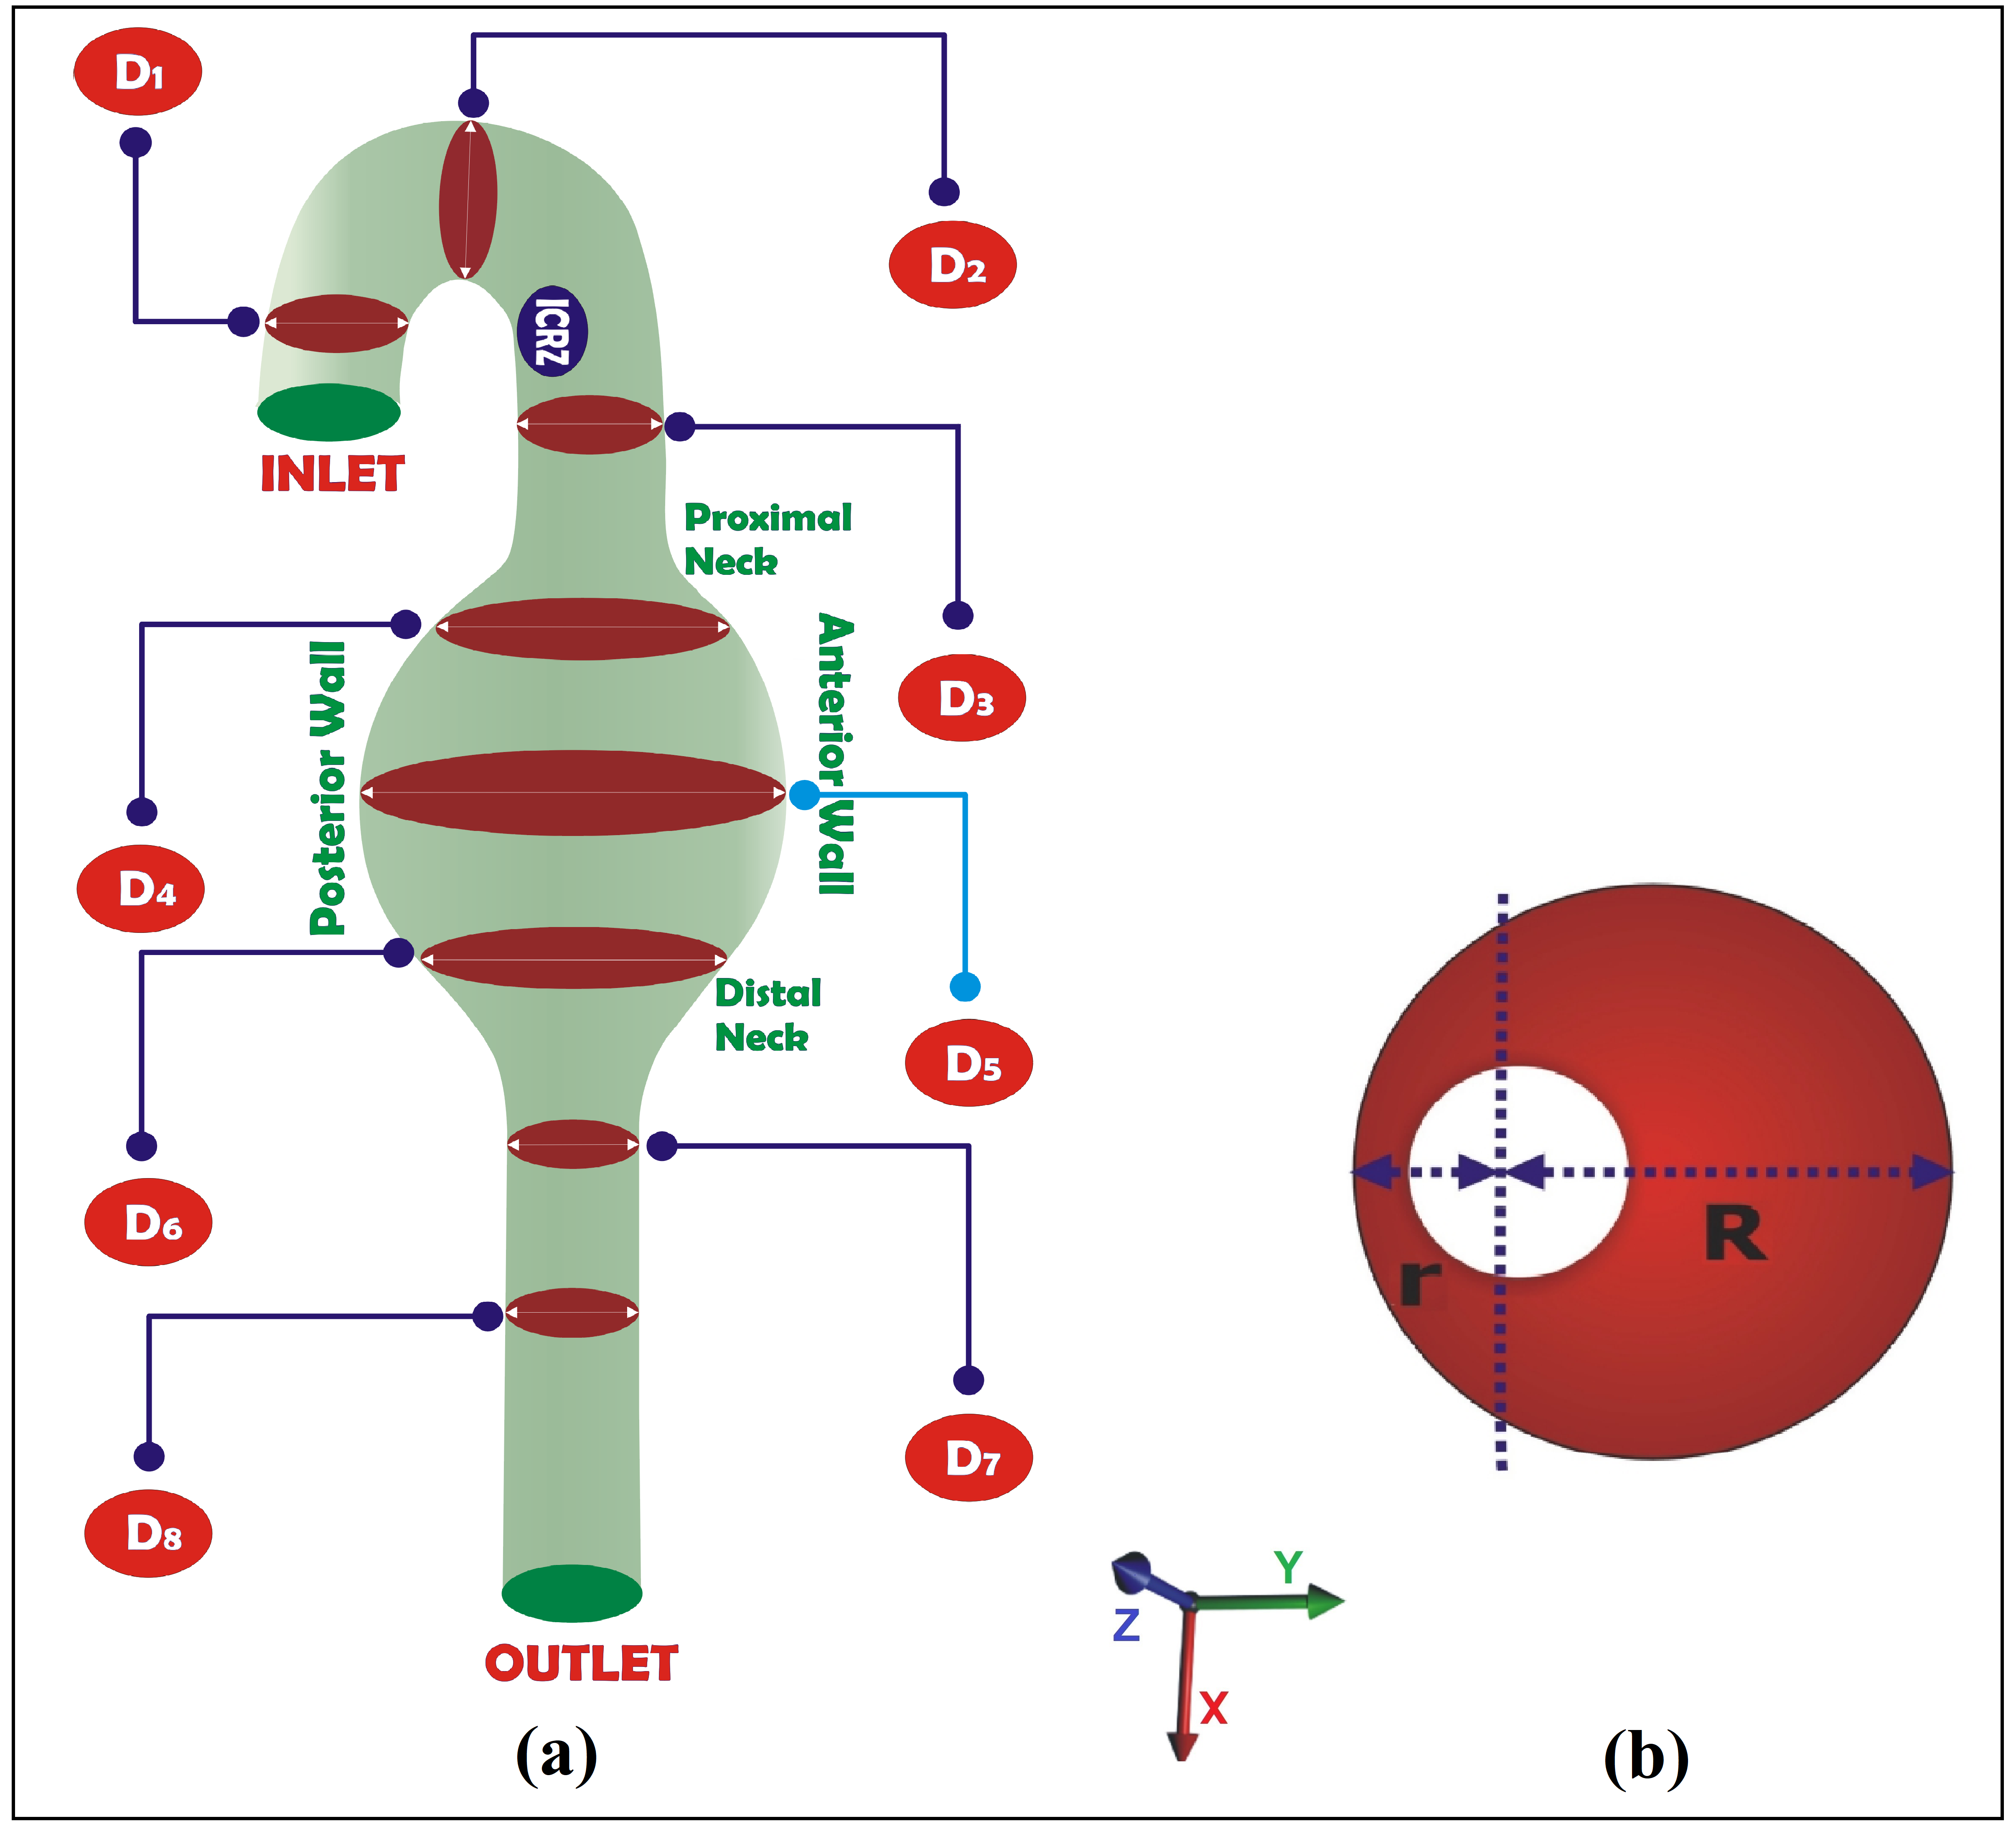
\includegraphics[width=1\textwidth, height=0.7\textheight]{Geometry.png}
         \caption{Visual depictions of (a) the three-dimensional geometry of the aneurysm and (b) the cross-sectional area of the aneurysm sac.}
         \label{fig:diagram}
     \end{figure}

     
\hspace*{\parindent} 

\subsection{\label{sec:governing_equations}Blood flow modeling and boundary conditions} 
\subsubsection{Governing equations and turbulence modeling}

The incompressible Navier--Stokes equations, which govern blood flow, are given by \cite{navier1823memoire, stokes2007theories}:
\begin{align}
    \nabla \cdot \mathbf{v} &= 0, \label{eq:cont}\\
    \rho \left( \frac{\partial \mathbf{v}}{\partial t} + (\mathbf{v} \cdot \nabla) \mathbf{v} \right) &= -\nabla p + \mu \nabla^2 \mathbf{v}, \label{eq:ns}
\end{align}
where \(\rho\) is the fluid density, \(\mathbf{v}\) the velocity vector, \(p\) the pressure, and \(\mu\) the dynamic viscosity.

For the unsteady Reynolds-averaged calculation, the instantaneous velocity will be decomposed as $\mathbf v=\mathbf V+\mathbf v'$ with $\overline{\mathbf v'}=0$, where $\mathbf V$ is the mean velocity. The Reynolds stress is closed by the Boussinesq eddy-viscosity approximation,
\begin{equation}
-\rho\overline{v_i'v_j'}=\mu_t\left(\partial_j V_i+\partial_i V_j\right)-\frac{2}{3}\rho k\delta_{ij},
\label{eq:boussinesq}
\end{equation}
where $k=\tfrac12\overline{v_i'v_i'}$ is \TKE per unit mass (m$^2$~s$^{-2}$), $\mu_t$ is dynamic eddy viscosity, and $\delta_{ij}$ is the Kronecker delta. With Eq.~\eqref{eq:boussinesq}, the Reynolds-averaged momentum equation solved for the mean velocity and pressure $P$ is
\begin{equation}
\rho\left(\frac{\partial\mathbf V}{\partial t}+(\mathbf V\cdot\nabla)\mathbf V\right)=-\nabla P+\nabla\cdot\left[(\mu+\mu_t)\left(\nabla\mathbf V+\nabla\mathbf V^{T}\right)\right]-\frac{2}{3}\nabla(\rho k),
\label{eq:urans}
\end{equation}
with $\nabla\cdot\mathbf V=0$.

\subsubsection{\texorpdfstring{\SSTcap \(k\)--\(\omega\) transition model}{SST k-omega transition model}}

The \SST \(k\)--\(\omega\) transition model was employed to account for the possible transition from laminar to turbulent flow and to capture the complex flow features associated with curvature, flow separation, and recirculation in the descending thoracic aorta. The model combines the near-wall formulation of the \(k\)--\(\omega\) model with the free-stream behavior of the \(k\)--\(\epsilon\) formulation through appropriate blending functions.

The turbulent eddy viscosity is calculated as
\begin{equation}
    \mu_t =
    \frac{a_1 \rho k}
    {\max(a_1\omega,\;SF_2)},
    \label{eq:mutt}
\end{equation}
where \(k\) is the \TKE, \(\omega\) is the specific dissipation rate, \(S\) is the magnitude of the strain-rate tensor, and \(F_2\) is the second blending function.

The transport equations for \TKE and specific dissipation rate are given by
\begin{equation}
\frac{\partial(\rho k)}{\partial t}
+\nabla\cdot(\rho k\mathbf{V})
=
\nabla\cdot
\left[
\left(\mu+\frac{\mu_t}{\sigma_k}\right)\nabla k
\right]
+P_k-D_k,
\label{eq:keqn}
\end{equation}

\begin{equation}
\frac{\partial(\rho\omega)}{\partial t}
+\nabla\cdot(\rho\omega\mathbf{V})
=
\nabla\cdot
\left[
\left(\mu+\frac{\mu_t}{\sigma_\omega}\right)\nabla\omega
\right]
+P_\omega-D_\omega
+
2(1-F_1)\rho\sigma_{\omega2}
\frac{1}{\omega}
\frac{\partial k}{\partial x_j}
\frac{\partial\omega}{\partial x_j}.
\label{eq:omegaeqn}
\end{equation}

Unlike the standard \SST \(k\)--\(\omega\) model, the transition formulation additionally solves two transport equations: one for the intermittency \(\gamma\), which varies from zero in laminar regions to unity in fully turbulent regions, and another for the transition momentum-thickness Reynolds number \(\widetilde{Re}_\theta\). These variables enable the model to predict the onset and development of boundary-layer transition based on the local flow conditions.

The blending functions \(F_1\) and \(F_2\) regulate the transition between the \(k\)--\(\omega\) and \(k\)--\(\epsilon\) formulations. \(F_1\) provides the appropriate near-wall blending, whereas \(F_2\) limits the eddy viscosity in regions where strain-rate effects become important. The distance to the nearest wall is denoted by \(y\). Thus, the \SST \(k\)--\(\omega\) transition model combines the strong near-wall behavior of the \(k\)--\(\omega\) formulation with the reduced free-stream sensitivity of the \(k\)--\(\epsilon\) formulation in the outer region of the boundary layer, while the additional intermittency and transition-Reynolds-number equations allow laminar--turbulent transition to be represented.




\subsubsection{Boundary conditions}
The pulsatile flow rate at the inlet is used in order to replicate the pulsatile nature of the blood flow in the human body. The inlet profile is expressed as:

\begin{equation}
Q(t)=
\begin{cases}
Q_0\,\sin\!\left(\dfrac{\pi\,(t-nT)}{0.35}\right)+0.05\,Q_0,
& nT \le t \le nT+0.35, \\[6pt]
0.05\,Q_0,
& nT+0.35 < t \le (n+1)T.
\end{cases}
\end{equation}


Similarly, the pulsatile outlet pressure is used at the outlet and is

\begin{equation}
P(t) =
\begin{cases} 
P_\mathrm{min} + \left(P_\mathrm{max} - P_\mathrm{min}\right) \, \sin\left(\dfrac{\pi \, (t - \, n \, T)}{0.35}\right), & nT \le t \le nT+0.35, \\
P_\mathrm{min}, & nT+0.35 < t \le (n+1)T.
\end{cases}
\end{equation}

Here $P_{\mathrm{min}}=80$~mmHg, $P_{\mathrm{max}}=120$~mmHg, $n=0,1,2,3$ indexes cardiac cycles, $T=0.8$~s, and $Q_0=2.39\times10^{-4}$~m$^3$~s$^{-1}$ is the sinusoidal amplitude. Because of the $0.05Q_0$ offset, the actual peak of the prescribed inlet flow rate is $1.05Q_0$.

{The inlet flow-rate and outlet pressure profiles that these two equations define are shown in Figure~\ref{fig:profiles}.}

\begin{figure}[!htb]
\centering
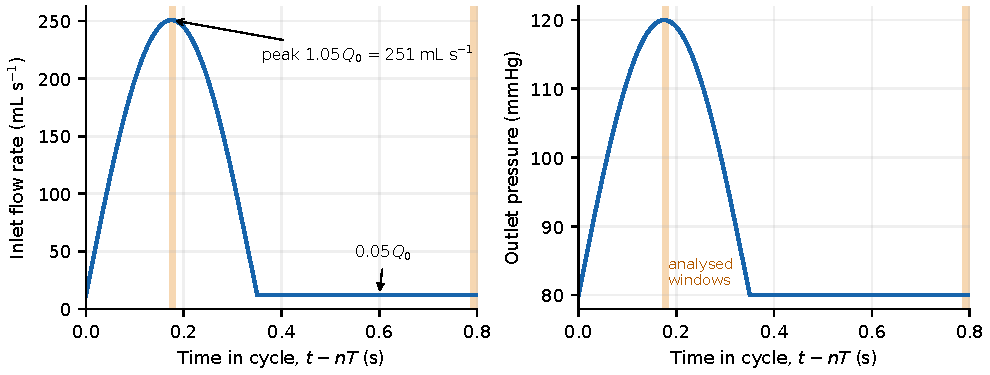
\includegraphics[width=\textwidth]{bc_profiles.pdf}
\caption{Prescribed inlet flow rate (left) and outlet pressure (right) over one cardiac cycle.}
\label{fig:profiles}
\end{figure}

At the wall no slip condition is applied.



\subsubsection{\label{sec:Hemodynamics Parameters}Hemodynamic parameters}

\hspace*{\parindent} \WSScap  denotes the tangential force per unit area applied by blood flow against the vessel wall. The \WSS for vessels \cite{potters2015volumetric} can be calculated using the formula:

\begin{align}
    \tau_w = \mu \left. \frac{\partial {u_t}}{\partial n} \right|_{n=0},
\end{align}

where \(\mu\) is the blood viscosity, \(\frac{\partial {u_t}}{\partial n}\) is the {tangential velocity gradient} in the direction \(n\) normal to the wall, and {\(u_t\) is the local tangential velocity component at the wall}.

To characterize the temporal and directional features of \WSS over a cardiac cycle, two additional metrics were computed on the aneurysm wall \cite{morbiducci2010outflow, turk2021characterization}:
\begin{equation}
\text{\TAWSScap} = \frac{1}{T} \int_{0}^{T} \left| \mathbf{WSS}(\mathbf{s},t) \right| \, dt,
\end{equation}
where $T$ is the duration of one cardiac cycle and $\mathbf{s}$ denotes a point on the vessel wall. \TAWSS  represents the magnitude of the \WSS vector averaged over time.

\TKEcap was quantified to assess the level of turbulence in the aneurysm sac, in addition to \WSS and \TAWSS. Here, \TKE represent the fluctuating components of the velocity field in the three coordinate directions. It provides an indicator of turbulence intensity and has been associated with increased flow instability and potential damage to the aneurysmal wall.

Additionally, velocity magnitudes were determined at eight predetermined cross-section planes (D1--D8) across the arterial axis and examined the spatial development of flow and its association with local vessel geometry. This was an analysis based on planes which allowed the direct correlation between morphometric parameters (diameter) and hemodynamic quantities (velocity, \TKE).


\MPScap was calculated on the inner surface of the aneurysmal wall to assess the structural response of the artery wall under pressure loading. \MPS represents the highest tensile principal stress at a given point and is commonly used in biomechanical studies as an indicator of rupture risk, because wall failure is expected when the local tensile stress exceeds the local tissue strength. The stress tensor was computed throughout the structural domain, and the spatial distribution of \MPS was analyzed to identify regions of elevated wall stress that may be more susceptible to mechanical failure.

\subsubsection{\label{CFD Simulation}\texorpdfstring{\CFDcap}{CFD} simulation}ANSYS Fluent, a commercial finite-volume solver with a pressure-based formulation, was used to solve the governing equations for mass and momentum conservation. Blood was modeled as an incompressible Newtonian fluid with density \(\rho = 1050\,\mathrm{kg\,m^{-3}}\) and dynamic viscosity \(\mu = 3.5 \times 10^{-3}\,\mathrm{Pa\,s}\).


The spatial convergence of the steady flow results was checked by performing a mesh refinement study. Prescribed flow rate was \(2.39 \times 10^{-4} \, \mathrm{m^3/s}\) and the \SST \(k\)-\(\omega\) turbulence model was used. Four different meshes (2.9~mm to 0.8~mm) were used in the testing as shown in (Table~\ref{tab:mesh_study}). The relative change, Richardson-extrapolated value and \GCI were computed between each mesh and the immediately finer mesh. The assumed second order convergence rate, $p=2$ was used in conjunction with Roache's conservative safety factor, $F_s=3.0$ for the evaluation of the \GCI. The two first refinements had relatively high \GCI values, which means that the coarser meshes were not in the range of mesh independent solution. For comparison, refinement from 1.3~mm to 0.8~mm changed the maximum aneurysmal \WSS by only 0.89\%, was Richardson extrapolated to 66.83~Pa, and had a fine-grid \GCI value of 1.63\%. Therefore, the 0.8~mm mesh was selected for the final simulations.

\begin{table}[ht!]
\centering
\setlength{\tabcolsep}{3.5pt}
\caption{Reported steady-flow fluid-mesh refinement for maximum aneurysmal \WSS. The extrapolation assumes second-order convergence.}
\label{tab:mesh_study}
\setlength{\tabcolsep}{7pt}
\begin{tabular}{cccccc}
\toprule
Element & Number of & Maximum & Relative & Richardson- & GCI$_{\rm fine}$ \\
size & elements & aneurysm & change & extrapolated & (\%) \\
(mm) & & \WSS (Pa) & (\%) & \WSS (Pa) & \\
\midrule
2.9 & 62\,261    & 47.8 & --    & --    & -- \\
1.9 & 196\,142   & 55.4 & 13.72 & 61.12 & 30.95 \\
1.3 & 578\,040   & 67.8 & 18.29 & 78.71 & 48.29 \\
0.8 & 1\,475\,430 & 67.2 & 0.89  & 66.83 & 1.63 \\
\bottomrule
\end{tabular}
\end{table}


The temporal convergence was evaluated for three different time step sizes: 0.01~s, 0.001~s, and 0.0005~s. The difference between the two smaller time steps was small, less than 2\%, and there was very good agreement in the \WSS waveforms. The time step was chosen as 0.001~s, which was found to be adequate in terms of both the level of temporal resolution and computational efficiency.

To eliminate initial transient effects and ensure a periodic steady state, the simulations were run for four consecutive cardiac cycles (\(n = 0,1,2,3\)). The percentage difference in \WSS between the third and fourth cycles was negligible (mean \(< 0.4\%\)), confirming that a periodic steady state had been reached. Accordingly, results from the third cardiac cycle were used for all subsequent analyses.



\subsubsection{Fluid--structure interaction model}

The arterial wall was modeled using ANSYS mechanical and considered as a nearly incompressible, isotropic hyperelastic material using the second-order Yeoh strain energy potential. The strain energy density function is
\begin{equation}
W = C_{10}(\bar{I}_1 - 3) + C_{20}(\bar{I}_1 - 3)^2,
\label{eq:yeoh}
\end{equation}
where \(W\) is the strain energy density, \(\bar{I}_1\) is the first deviatoric strain invariant, and \(C_{10}\) and \(C_{20}\) are material constants. The material constants were set to \(C_{10} = 98.8~\text{kPa}\) and \(C_{20} = 779.1~\text{kPa}\) \cite{zhu2025combined}. The incompressibility parameter \(D_1\) was specified as \(2.04 \times 10^{-4}~\text{kPa}^{-1}\), corresponding to a Poisson's ratio of \(\nu = 0.49\). A uniform wall thickness of 2.0~mm was assumed for all models, consistent with previous idealized \FSI studies of thoracic \AANs, and the arterial wall density was set to 1120~kg/m\(^3\).

To represent the physiological fixation of the artery, fixed boundary conditions were applied at both the inlet and outlet. The \FSI  interface was defined on the inner surface of the arterial wall to enable bidirectional coupling between the fluid and structural domains. The computational workflow is presented in Figure~\ref{fig:Flowchart}.



\begin{figure}[!ht]
  \centering
  \definecolor{cIn}{HTML}{1F6FB2}
  \definecolor{cNet}{HTML}{0E8C84}
  \definecolor{cData}{HTML}{C0392B}
  \definecolor{cPhys}{HTML}{B07A12}
  \definecolor{cPost}{HTML}{2E7D32}
  \definecolor{cOpt}{HTML}{555555}
  \resizebox{\textwidth}{!}{%
  \begin{tikzpicture}[
      font=\small,
      >={Stealth[length=2.2mm]},
      box/.style={rounded corners=2pt, draw=#1!70, line width=0.6pt, fill=#1!7,
                  align=center, inner sep=4pt, text=black, minimum width=52mm, minimum height=9mm},
      dec/.style={diamond, aspect=2.2, draw=cOpt!70, fill=cOpt!7, line width=0.6pt, inner sep=1.5pt, font=\small},
      arr/.style={->, draw=black!65, line width=0.7pt},
      lab/.style={font=\footnotesize, text=black!70},
      ilab/.style={font=\footnotesize\itshape, text=black!60},
    ]

    % ---------------------------------------------------------
    % Top: geometry
    % ---------------------------------------------------------
    \node[box=cOpt, minimum width=60mm] (geo) {\textbf{Geometry}: Twelve idealized models};

    % ---------------------------------------------------------
    % Left column: fluid
    % ---------------------------------------------------------
    \node[box=cIn, below left=8mm and -14mm of geo] (fl) {\textbf{Fluid (blood)}: ANSYS Fluent};
    \node[box=cIn, below=4mm of fl] (fmesh) {Mesh generation};
    \node[box=cIn, below=4mm of fmesh, align=center] (fset) {%
        Fluid properties and boundary conditions.\\
        Discretization method and convergence setup.};
    \node[dec, below=5mm of fset] (conv) {converged?};
    \node[box=cIn, below=6mm of conv] (fres) {Results};

    \draw[arr] (fl) -- (fmesh);
    \draw[arr] (fmesh) -- (fset);
    \draw[arr] (fset) -- (conv);
    \draw[arr] (conv) -- node[lab, right]{yes} (fres);

    \coordinate (loopx) at ($(fset.west)+(-5mm,0)$);
    \draw[arr] (conv.west) -- node[lab, above]{no} (conv.west -| loopx) |- (fset.west);

    % ---------------------------------------------------------
    % Right column: solid
    % ---------------------------------------------------------
    \node[box=cPost, below right=8mm and -14mm of geo] (so) {\textbf{Solid (wall)}: ANSYS Mechanical};
    \node[box=cPost, below=4mm of so] (smesh) {Mesh generation};
    \node[box=cPost, below=4mm of smesh, align=center] (sset) {%
        Wall properties and boundary conditions.};
    \node[box=cPost, below=4mm of sset] (sa) {Stress analysis};
    \node[box=cPost, below=4mm of sa] (sres) {Results};
    \node[box=cPost, below=4mm of sres] (end) {End};

    \draw[arr] (so) -- (smesh);
    \draw[arr] (smesh) -- (sset);
    \draw[arr] (sset) -- (sa);
    \draw[arr] (sa) -- (sres);
    \draw[arr] (sres) -- (end);

    % ---------------------------------------------------------
    % Links from geometry to both columns
    % ---------------------------------------------------------
    \draw[arr] (geo.south) -- ++(0,-3mm) -| (fl.north);
    \draw[arr] (geo.south) -- ++(0,-3mm) -| (so.north);

    % ---------------------------------------------------------
    % Wall-pressure transfer from fluid to solid
    % ---------------------------------------------------------
    \coordinate (cpx) at ($(fset.east)!0.5!(fset.east -| sa.west)$);
    \draw[arr, draw=cPhys!90, line width=0.9pt]
          (fres.east) -- (fres.east -| cpx) -- (cpx |- sa.west) -- (sa.west);
    \node[lab, text=cPhys!90!black, rotate=90, anchor=north, inner sep=1pt]
          at ($(fres.east -| cpx)!0.5!(cpx |- sa.west)$) {wall pressure};

  \end{tikzpicture}%
  }
  \caption{\CFDcap and structural workflow. The fluid problem is solved in ANSYS Fluent, and the wall pressure is transferred to the structural model in ANSYS Mechanical.}
  \label{fig:Flowchart}
\end{figure}



\section{Sparse-velocity reconstruction methods}
\label{sec:reconstruction_methods}
\subsection{Exported flow fields, instants and regions}
\label{sec:exports}
All quantitative flow results in this paper, including the reconstruction study, use whole-domain exports of the rigid-wall \CFD solutions rather than the structural calculation. For each case the exports contain every fluid node (468\,000--603\,000 interior nodes and 34\,600--41\,400 wall nodes) with velocity, static pressure, eddy viscosity $\mu_t$, $k$ and $\omega$, together with the \WSS vector on the wall nodes and the inlet and outlet faces. The mesh and node ordering are identical across the snapshots of a case, so differences between snapshots are exact nodal differences. No cell volumes, face areas or connectivity were exported, and all averages are therefore node-weighted. The near-wall node spacing differs between the two groups of models. In the aneurysmal models the interior node nearest each wall node lies a median 0.03--0.04~mm from the wall in the aneurysm zone but 0.58~mm on the rest of the wall, including the bend, whereas in the controls it lies 0.04~mm from the wall everywhere. Near-wall refinement in the aneurysmal models is therefore confined to the aneurysm zone, and quantities outside that zone, including comparisons with the controls there, depend on near-wall resolution as well as on geometry.

Snapshots exist for every case at 1.780~s and at 2.390 and 2.400~s, and for all cases except Case~2 at 1.775~s; Case~2 instead has a snapshot at 1.788~s, which completes its systolic window. Peak inflow occurs at 1.775~s, $0.175$~s into the third cycle, so 1.780~s is 5~ms after the peak, and 2.400~s is the end of the diastolic plateau of the third cycle. We use 1.780~s and 2.400~s as common systolic and diastolic instants and refer to them below as the systolic and diastolic phases. All exported fields were post-processed and plotted with Python scripts (NumPy, SciPy and Matplotlib). The earlier case-specific image exports were taken at different near-systolic times (1.775--1.815~s), and they are used only as qualitative illustrations.

Two regions are used throughout. The \emph{aneurysm zone} is the wall zone exported as the dilation for each aneurysmal case, which spans the sac and its necks. For comparisons that include the controls, the \emph{dilation segment} is the axial extent of the aneurysm zone of the axisymmetric case with the same inlet diameter, restricted to the descending branch, so that each control is evaluated over the corresponding stretch of undilated vessel. Within the straight descending segment the global $x$ axis coincides with the local downstream direction, which makes a negative $x$ velocity a meaningful indicator of reversed flow there, unlike in the curved inlet region.


\subsection{Task and information available to each method}
\label{sec:task}
Each reconstruction problem concerns one geometry and one short window of two snapshots. The systolic window is 1.775--1.780~s, with the target at 1.780~s, except for Case~2, which has no 1.775~s export and uses 1.780--1.788~s with the same target. The diastolic window is 2.390--2.400~s, with the target at 2.400~s. Given velocity at a sparse set of interior nodes at both window times, a method must recover velocity at all other interior nodes, the gauge pressure in the interior and the \WSS magnitude on the aneurysm zone at the target time. The geometry is known, so the task is reconstruction within a given anatomy rather than prediction for a new one.

Table~\ref{tab:information} lists what each method may use. Geometry comprises the coordinates of the interior nodes without their field values, the wall nodes with inward normals, and the inlet and outlet faces. Boundary information comprises the prescribed inlet velocity and the mean outlet pressure at each window time. Pressure, \WSS and velocity at unobserved nodes are never used for fitting or selection. We examine two viscosity settings. The first supplies the \CFD eddy-viscosity field $\mu_t$ and its spatial gradient, so the momentum balance uses $\mu+\mu_t$. We call this the \emph{oracle} setting because it gives the reconstruction access to closure information from the reference simulation. The second uses only the prescribed blood viscosity, $\mu=3.5\times10^{-3}$~Pa~s, with $\mu_t=0$; this is the \emph{molecular-viscosity} setting. The \CFD eddy viscosity is not measured by the sparse velocity observations. Results that use it are therefore conditional on that additional information.

\begin{table}[htbp]
\centering
\small
\caption{Information used by each method. All methods receive the same observation nodes at both window times and are scored through the same post-processing.}
\label{tab:information}
\setlength{\tabcolsep}{4pt}
\begin{tabular}{p{4.3cm}ccccc}
\toprule
Information & Linear & \RBF & \shortstack{Data\\field} & \shortstack{Continuity\\field} & \shortstack{Momentum\\\PINN} \\
\midrule
Sparse velocity at two times & \checkmark & \checkmark & \checkmark & \checkmark & \checkmark \\
Wall no-slip and inlet velocity & \checkmark & \checkmark & \checkmark & \checkmark & \checkmark \\
Outlet pressure datum & post-proc. & post-proc. & \checkmark & \checkmark & \checkmark \\
Interior node coordinates (no values) & -- & -- & -- & \checkmark & \checkmark \\
Continuity in the fit & -- & -- & -- & \checkmark & \checkmark \\
Momentum balance in the fit & -- & -- & -- & -- & \checkmark \\
\CFDcap $\mu_t$ (oracle setting) & post-proc. & post-proc. & post-proc. & post-proc. & fit + post-proc. \\
\bottomrule
\end{tabular}
\end{table}

\subsection{Observation design}
\label{sec:observations}
Velocity is observed at the interior nodes nearest to the points of a uniform Cartesian grid with spacing $\Delta$ and a random offset, keeping only grid points with an interior node within $\Delta/2$. The same nodes are observed at both window times. Sampling on a grid rather than on mesh nodes avoids oversampling the refined near-wall layers. Each grid point is, however, snapped to a mesh node, so observations next to the wall fall on the prism layers. At $\Delta=2.5$~mm, 5.6--8.5\% of the observed nodes of Cases~2--8 lie within 0.25~mm of the wall and 26--30\% within 1~mm, the closest at 0.03~mm, whereas a 2.5~mm imaging voxel would return an average over its volume. The design is therefore point sampling on a grid rather than voxel sampling. Every method receives the same observations, so the comparison between methods is not affected, but the absolute \WSS errors are optimistic relative to imaging data; Section~\ref{sec:nearwall} quantifies this by removing the near-wall observations. The primary spacing $\Delta=2.5$~mm observes 1.27--1.36\% of the interior nodes per time (5\,970--8\,205 nodes), and the secondary spacings of 1.5 and 4.0~mm observe 5.4--5.8\% and 0.34--0.37\%. The observed values are noise-free \CFD values at mesh nodes. A random 10\% of the observed nodes is withheld from fitting and used only for model selection and monitoring. Each draw $s$ fixes both the grid offset and the network initialization, draws are paired across methods, and the observed node indices are stored.


\subsection{Space-time neural fields and physics constraints}
\label{sec:field}
We use a space-time neural field to represent each short flow window. The confirmation method is a continuity-constrained field followed by physics-based post-processing, in which the network reconstructs velocity and separate calculations recover pressure and \WSS. We refer to this method as the continuity field. Its divergence penalty is a physical constraint, but it does not enforce the momentum balance during fitting. We use the term \emph{momentum \PINN} for the separate arms, tested only on the two development geometries, that also penalize the momentum residual. 

All neural arms share the same architecture, which maps position and time to velocity and pressure, $(\mathbf x,t)\mapsto(\mathbf u_\theta,p_\theta)$. Coordinates are scaled as $\mathbf x_s=(\mathbf x-\mathbf x_c)/L$, where $\mathbf x_c$ is the centroid of the interior nodes and $L$ is half the largest extent of the domain, and time is mapped to $t_s\in[-1,1]$ across the window. Velocity is scaled by $U$, the 99.5th percentile of observed speed at the target time, and pressure by $\rho U^2$. The input is $[\sin(2\pi\mathbf B^{\mathsf T}\mathbf x_s),\cos(2\pi\mathbf B^{\mathsf T}\mathbf x_s),\mathbf x_s,t_s]$, where $\mathbf B\in\mathbb R^{3\times64}$ holds Gaussian Fourier features with a \SD of 2~\cite{tancik2020fourier}, followed by six fully connected layers of width 256 with SiLU activations and a linear output of four scaled quantities (about 360\,000 parameters) (Figure~\ref{fig:network}).

\begin{figure}[!t]
  \centering
  \definecolor{cIn}{HTML}{1F6FB2}
  \definecolor{cEnc}{HTML}{6A4C93}
  \definecolor{cNet}{HTML}{0E8C84}
  \definecolor{cData}{HTML}{C0392B}
  \definecolor{cPhys}{HTML}{B07A12}
  \definecolor{cBC}{HTML}{2E7D32}
  \definecolor{cOpt}{HTML}{555555}
  \resizebox{\textwidth}{!}{%
  \begin{tikzpicture}[
      font=\small,
      >={Stealth[length=2.2mm]},
      box/.style={rounded corners=2pt, draw=#1!70, line width=0.6pt, fill=#1!7,
                  align=center, inner sep=3.5pt, text=black},
      box/.default=black,
      inp/.style={box=cIn,  minimum width=24mm, minimum height=9mm},
      enc/.style={box=cEnc, minimum width=30mm, minimum height=10mm},
      cat/.style={draw=black!55, fill=black!6, circle, inner sep=1.5pt, minimum size=13mm, align=center},
      outn/.style={circle, draw=#1!75, fill=#1!16, line width=0.6pt, minimum size=7.5mm,
                  inner sep=0pt, font=\footnotesize},
      loss/.style={box=#1, minimum width=40mm, minimum height=12mm},
      opt/.style={box=cOpt, minimum width=36mm, minimum height=10mm},
      neuron/.style={circle, draw=cNet!70, fill=cNet!12, minimum size=3.4mm, inner sep=0pt},
      edge/.style={draw=cNet!35, line width=0.25pt},
      arr/.style={->, draw=black!65, line width=0.7pt},
      bus/.style={draw=black!60, line width=0.7pt},
      lab/.style={font=\footnotesize, text=black!70},
      ilab/.style={font=\footnotesize\itshape, text=black!60},
    ]
    \node[inp] (x) {$\mathbf{x}=(x,y,z)$};
    \node[inp, below=12mm of x] (t) {$t\in[t_o,t_\star]$};
    \node[lab, left=1mm of x] (lx) {position};
    \node[lab, left=1mm of t] (lt) {time};
    \node[enc, right=10mm of x] (fF) {Fourier features $\gamma(\mathbf{x}_s)$\\{\footnotesize 64 frequencies, $\sigma=2$}};
    \node[enc, right=10mm of t] (ts) {window scaling\\{\footnotesize $t_s\in[-1,1]$}};
    \coordinate (mid) at ($(fF.east)!0.5!(ts.east)$);
    \node[cat, right=9mm of mid] (cat) {\scriptsize concat\\[-1pt]\scriptsize $[\gamma,\mathbf{x}_s,t_s]$};
    \draw[arr] (x) -- (fF);
    \draw[arr] (t) -- (ts);
    \draw[arr] (fF.east) -- ([yshift= 2mm]cat.west);
    \draw[arr] (ts.east) -- ([yshift=-2mm]cat.west);

    \coordinate (netorg) at ($(cat.east)+(27mm,0)$);
    \begin{scope}[shift={(netorg)}]
      \node[rounded corners=3pt, draw=cNet!70, fill=white, minimum width=38mm, minimum height=27mm] (mlp) {};
      \foreach \i in {1,2,3}\node[neuron] (a\i) at (-15mm, {(\i-2)*6mm}) {};
      \foreach \i in {1,2,3,4}\node[neuron] (b\i) at (-5mm, {(\i-2.5)*5mm}) {};
      \foreach \i in {1,2,3,4}\node[neuron] (c\i) at (5mm,  {(\i-2.5)*5mm}) {};
      \node[neuron] (d1) at (15mm,0) {};
      \foreach \i in {1,2,3}\foreach \j in {1,2,3,4}\draw[edge] (a\i)--(b\j);
      \foreach \i in {1,2,3,4}\foreach \j in {1,2,3,4}\draw[edge] (b\i)--(c\j);
      \foreach \i in {1,2,3,4}\draw[edge] (c\i)--(d1);
    \end{scope}
    \node[ilab, text=cNet!80, below=1.5mm of mlp] (mlplab) {6 layers $\times$ 256 units, SiLU};
    \draw[arr] (cat.east) -- (a2);

    \node[outn=cIn, right=15mm of mlp, yshift=11.5mm] (ou) {$u$};
    \node[outn=cIn, below=2.2mm of ou] (ov) {$v$};
    \node[outn=cIn, below=2.2mm of ov] (ow) {$w$};
    \node[outn=cPhys, below=2.2mm of ow] (op) {$p$};
    \foreach \o in {ou,ov,ow,op}{\draw[arr] (d1) -- (\o);}
    \draw[decorate, decoration={brace, amplitude=3pt, raise=1pt}, draw=black!50, line width=0.5pt]
      ($(ou.east)+(1.5mm,0)$) -- ($(ow.east)+(1.5mm,0)$);
    \node[lab, anchor=west] (lvel) at ($(ov.east)+(5.5mm,0)$) {velocity};
    \node[lab, anchor=west] (lpre) at (lvel.west |- op) {pressure};

    \begin{scope}[on background layer]
      \node[rounded corners=4pt, draw=black!40, fill=black!1.5,
            fit=(lx)(lt)(x)(t)(fF)(ts)(cat)(mlp)(mlplab)(ou)(op)(lvel)(lpre), inner sep=5mm] (net) {};
    \end{scope}
    \node[ilab, anchor=south west, text=black!65] at ($(net.north west)+(1.5mm,0.8mm)$)
         {Network $f_\theta(\mathbf{x},t)$, fitted separately for each case and window};

    \node[loss=cPhys] (phys) at ($(net.south)+(0,-16mm)$)
         {\textbf{Physics}, weight $w=0.01$\\continuity $\nabla\!\cdot\mathbf{u}$\\{\footnotesize\color{black!60}momentum \PINNs: + momentum residual}};
    \node[loss=cData, left=10mm of phys] (data)
         {\textbf{Data}\\$\mathbf{u}$ at observed nodes, $t_o$ and $t_\star$};
    \node[loss=cBC, right=10mm of phys] (bc)
         {\textbf{Boundary}\\no-slip, inlet $\mathbf{u}$, outlet datum};
    \coordinate (busL) at ($(net.south)+(0,-6mm)$);
    \draw[bus] (net.south) -- (busL);
    \node[ilab, anchor=south west, text=black!70] at ($(net.south)+(1.8mm,-1mm)$) {predictions};
    \draw[bus] (busL) -| (data.north);
    \draw[arr] (busL) -- (phys.north);
    \draw[bus] (busL) -| (bc.north);
    \draw[arr] ($(data.north)+(0,2mm)$)--(data.north);
    \draw[arr] ($(bc.north)+(0,2mm)$)--(bc.north);

    \node[opt, minimum width=48mm] (sum) at ($(phys.south)+(0,-11mm)$) {$\mathcal L=\mathcal L_{\rm data}+\mathcal L_{\rm bc}+w\,\mathcal L_{\rm phys}$};
    \node[opt, below=6mm of sum] (adam) {Adam, lr $10^{-3}\!\to\!10^{-5}$ (cosine),\\20\,000 steps, gradient clipping};
    \draw[arr] (data.south) |- (sum.west);
    \draw[arr] (phys.south) -- (sum.north);
    \draw[arr] (bc.south) |- (sum.east);
    \draw[arr] (sum.south) -- (adam.north);
    \coordinate (fbmid) at ([xshift=7mm]net.east);
    \coordinate (fbbot) at (fbmid |- adam.east);
    \draw[arr, dashed, draw=black!55] (adam.east) -- (fbbot)
       -- node[lab, pos=0.55, right]{$\nabla_\theta$} (fbmid) -- (net.east);
  \end{tikzpicture}%
  }
  \caption{Space-time neural field. Fourier-encoded position and scaled time pass through a fully connected network to velocity and pressure, fitted to the observed velocity and the boundary conditions. The continuity arm adds a divergence penalty; the momentum residual (gray) was used only by the momentum \PINNs tested on the two development geometries.}
  \label{fig:network}
\end{figure}


The loss combines data and boundary terms with an optional physics term,
\begin{equation}
\mathcal L=\mathcal L_{\rm obs}+\mathcal L_{\rm wall}+\mathcal L_{\rm in}+\mathcal L_{\rm out}+w\,\mathcal L_{\rm phys},
\label{eq:loss}
\end{equation}
where $\mathcal L_{\rm obs}$ is the mean squared velocity misfit at the observed nodes at both times, $\mathcal L_{\rm wall}$ penalizes velocity at wall nodes at random times in the window, $\mathcal L_{\rm in}$ penalizes the misfit to the prescribed inlet velocity at each window time, and $\mathcal L_{\rm out}$ penalizes the squared mean of $p_\theta$ on the outlet face, which fixes the pressure datum. Four arms differ only in $\mathcal L_{\rm phys}$. The \emph{data} arm has none. The \emph{continuity} arm uses the mean squared divergence $(\nabla\cdot\mathbf u_\theta)^2$ at interior nodes drawn at random times. The \emph{steady} and \emph{unsteady} momentum arms add the mean squared residual of
\begin{equation}
\rho\,\partial_t\mathbf u+\rho(\mathbf u\cdot\nabla)\mathbf u
+\nabla p-\nabla\cdot\left[(\mu+\mu_t)
(\nabla\mathbf u+\nabla\mathbf u^{\mathsf T})\right]=\mathbf 0,
\label{eq:momentum}
\end{equation}
without the time term in the steady arm, with $\mu_t$ interpolated linearly in time between the two snapshots in the oracle setting and set to zero in the molecular setting. Derivatives are taken by automatic differentiation, and the variable-viscosity divergence retains the gradient of $\mu_t$. Equation~\eqref{eq:momentum} has no separate $2\rho k/3$ term because the exported \CFD pressure satisfies the momentum balance better without it (Section~\ref{sec:reference_results}), indicating that the isotropic turbulent stress is already contained in the exported pressure.

Each step draws 4096 observations, 4096 collocation nodes, 2048 wall nodes, 512 inlet nodes per time and 256 outlet nodes per time. Training uses Adam with a learning rate of $10^{-3}$, cosine decay to $10^{-5}$ over 20\,000 steps and gradient-norm clipping at 1. There is no early stopping, and the last iterate is scored. The physics weight $w$ was chosen for each arm from $\{0.01,0.1,1\}$ on Case~1 at systole by the error on the withheld observations and then frozen. That error increased with $w$ in every arm, so $w=0.01$ was used throughout. On one NVIDIA Quadro RTX 8000 shared with other jobs, a 20\,000-step fit took a median of 23~min for the continuity arm and 17~min for the data arm.

\subsection{Interpolation comparators}
\label{sec:interpolation}
The comparators interpolate the same observations, with zero velocity at the wall nodes and the prescribed inlet velocity added as sources, separately at each window time. \emph{Linear} interpolation uses the Delaunay triangulation of the sources, with the nearest source used outside its hull. \emph{\RBF} interpolation uses a local thin-plate-spline \RBF with a linear polynomial on the 64 nearest sources, which is widened to 128 sources only where a neighborhood is coplanar and the local system is singular. These settings were fixed before the development test and are the prespecified comparator. Two further comparators were added after the confirmatory verdict as robustness checks. The \emph{tuned \RBF} selects the kernel (thin-plate spline, cubic or quintic), the neighborhood size (32--256) and the smoothing parameter ($0$--$10^{-2}$) by the error on the withheld observations. The \emph{space-time \RBF} fits one interpolant over $(\mathbf x, c\,t)$ through both snapshots, with the time scale $c\in\{0,0.5,2,8\}$~m~s$^{-1}$, the kernel and the neighborhood size chosen on the same withheld observations.

\subsection{Shared post-processing}
\label{sec:postprocessing}
Every reconstruction, including the complete \CFD velocity used as a reference, is converted to pressure and \WSS by the same steps (Figure~\ref{fig:pipeline}). The reconstructed velocity is first sampled at the \CFD nodes. Spatial gradients are computed by weighted least squares on the 40 nearest nodes with inverse-square-distance weights, with zero velocity imposed at the wall nodes. The momentum balance then gives a target pressure gradient,
\begin{equation}
\mathbf f=-\rho\,\frac{\mathbf u(t_\star)-\mathbf u(t_o)}{t_\star-t_o}
-\rho(\mathbf u\cdot\nabla)\mathbf u
+\nabla\cdot\left[(\mu+\mu_t)(\nabla\mathbf u+\nabla\mathbf u^{\mathsf T})\right],
\label{eq:pressure_rhs}
\end{equation}
evaluated at the target time $t_\star$, where $t_o$ is the other window time. The gauge pressure is the least-squares solution of $\nabla_h p=\mathbf f$ on the interior nodes more than 1~mm from the wall, with the mean pressure over nodes beyond $x=0.130$~m set to zero, computed with LSQR. Near-wall nodes are excluded because the prism-layer stencils are poorly conditioned. Dropping the first term of Eq.~\eqref{eq:pressure_rhs} gives the steady form, and setting $\mu_t=0$ gives the molecular form. All four combinations are reported, and the unsteady form with oracle $\mu_t$ is the prespecified pressure endpoint. The steady form of Eq.~\eqref{eq:pressure_rhs} is the standard pressure-gradient route of velocity-based relative-pressure estimation~\cite{bertoglio2018relative}.

\WSScap is estimated at each aneurysm-zone wall node $\mathbf x_w$ with inward unit normal $\mathbf n$ from the tangential velocity $\mathbf u_t$ at two distances inside the lumen,
\begin{equation}
\boldsymbol\tau_w\approx\mu\,\frac{4\,\mathbf u_t(\mathbf x_w+h\mathbf n)-\mathbf u_t(\mathbf x_w+2h\mathbf n)}{2h},
\label{eq:wss_estimate}
\end{equation}
which is second-order accurate for a no-slip wall, with $\mathbf u_t$ obtained by linear interpolation of the nodal velocity. The prespecified distance is $h=0.25$~mm, and results at 0.1 and 0.5~mm are reported only as an oracle sensitivity. In the aneurysm zone the interior node nearest the wall lies a median 0.03--0.04~mm from it, so Eq.~\eqref{eq:wss_estimate} is informative there. Outside the aneurysm zone that distance is 0.58~mm, and even the complete \CFD velocity reproduces the exported \WSS there only to a relative error of 0.46--0.68, so \WSS outside the aneurysm zone is not used as a target.


\begin{figure}[!t]
  \centering
  \definecolor{cIn}{HTML}{1F6FB2}
  \definecolor{cNet}{HTML}{0E8C84}
  \definecolor{cData}{HTML}{C0392B}
  \definecolor{cPhys}{HTML}{B07A12}
  \definecolor{cPost}{HTML}{2E7D32}
  \definecolor{cOpt}{HTML}{555555}
  % outline of an idealized aneurysmal segment, used by the pictograms below
  \def\vesselpath{(-1.1,0.22) -- (-0.45,0.22) .. controls (-0.25,0.62) and (0.25,0.62) .. (0.45,0.22)
    -- (1.1,0.22) -- (1.1,-0.22) -- (0.45,-0.22) .. controls (0.25,-0.62) and (-0.25,-0.62) .. (-0.45,-0.22)
    -- (-1.1,-0.22) -- cycle}
  \resizebox{\textwidth}{!}{%
  \begin{tikzpicture}[
      font=\small,
      >={Stealth[length=2.2mm]},
      card/.style={rounded corners=3pt, draw=#1!70, line width=0.6pt, fill=#1!6},
      ttl/.style={font=\small\bfseries, text=black, align=center},
      sub/.style={font=\footnotesize, text=black!72, align=center},
      arr/.style={->, draw=black!60, line width=0.7pt},
      ln/.style={draw=black!60, line width=0.7pt},
      step/.style={circle, fill=#1, text=white, font=\footnotesize\bfseries, inner sep=0pt, minimum size=4.8mm},
      steplab/.style={font=\small\bfseries, text=black!75, anchor=west},
      % ---------- pictograms ----------
      obsicon/.pic={
        \draw[cIn!70, line width=0.6pt, fill=white] \vesselpath;
        \foreach \x in {-0.9,-0.6,...,0.95}{\fill[cIn] (\x,0.1) circle (0.045); \fill[cIn] (\x,-0.1) circle (0.045);}
        \foreach \x in {-0.2,0.1}{\fill[cIn] (\x,0.36) circle (0.045); \fill[cIn] (\x,-0.36) circle (0.045);}
      },
      linicon/.pic={
        \draw[cOpt!80, line width=0.45pt, fill=cOpt!10]
          (0,0) -- (0.5,0.08) -- (0.22,0.45) -- cycle (0.5,0.08) -- (0.78,0.46) -- (0.22,0.45)
          (0,0) -- (-0.28,0.36) -- (0.22,0.45);
        \foreach \p in {(0,0),(0.5,0.08),(0.22,0.45),(0.78,0.46),(-0.28,0.36)}{\fill[cIn] \p circle (0.05);}
      },
      rbficon/.pic={
        \draw[cOpt!45, line width=0.4pt] (-0.45,0) -- (0.85,0);
        \draw[cOpt!85, line width=0.7pt, domain=-0.45:0.85, samples=50, smooth]
          plot (\x,{0.45*exp(-((\x+0.02)^2)/0.03)+0.28*exp(-((\x-0.45)^2)/0.02)});
        \fill[cIn] (-0.02,0.45) circle (0.05); \fill[cIn] (0.45,0.29) circle (0.05);
      },
      nnicon/.pic={
        \foreach \a in {-0.22,0,0.22}{\foreach \b in {-0.33,-0.11,0.11,0.33}{\draw[cNet!35, line width=0.3pt] (0,\a) -- (0.4,\b);}}
        \foreach \b in {-0.33,-0.11,0.11,0.33}{\draw[cNet!35, line width=0.3pt] (0.4,\b) -- (0.8,0.1); \draw[cNet!35, line width=0.3pt] (0.4,\b) -- (0.8,-0.1);}
        \foreach \a in {-0.22,0,0.22}{\fill[cNet] (0,\a) circle (0.05);}
        \foreach \b in {-0.33,-0.11,0.11,0.33}{\fill[cNet] (0.4,\b) circle (0.05);}
        \fill[cNet] (0.8,0.1) circle (0.05); \fill[cNet] (0.8,-0.1) circle (0.05);
      },
      velicon/.pic={
        \draw[cIn!70, line width=0.6pt, fill=white] \vesselpath;
        \foreach \x in {-0.95,-0.65,0.45,0.75}{\draw[->, >={Stealth[length=0.8mm]}, cIn, line width=0.45pt] (\x,0) -- ++(0.24,0);}
        \draw[->, >={Stealth[length=0.8mm]}, cIn, line width=0.45pt] (-0.3,0) -- ++(0.55,0);
        \draw[->, >={Stealth[length=0.8mm]}, cData!80, line width=0.45pt] (0.12,0.36) -- ++(-0.22,0);
        \draw[->, >={Stealth[length=0.8mm]}, cData!80, line width=0.45pt] (0.12,-0.36) -- ++(-0.22,0);
      },
      cfdicon/.pic={
        \draw[cOpt!60, line width=0.6pt, fill=white] \vesselpath;
        \foreach \y in {-0.12,0,0.12}{\draw[cOpt!55, line width=0.35pt] (-1.05,\y) .. controls (-0.3,\y) and (0.3,\y) .. (1.05,\y);}
        \draw[cOpt!55, line width=0.35pt] (-0.15,0.3) ellipse (0.18 and 0.08);
        \draw[cOpt!55, line width=0.35pt] (-0.15,-0.3) ellipse (0.18 and 0.08);
      },
      presicon/.pic={
        \shade[left color=cData!60, right color=cIn!45] \vesselpath;
        \draw[black!45, line width=0.5pt] \vesselpath;
        \node[font=\tiny\bfseries, text=white] at (-0.72,0) {$+$};
        \node[font=\tiny\bfseries, text=black!70] at (0.72,0) {$-$};
      },
      wssicon/.pic={
        \foreach \x in {-0.5,-0.36,...,0.62}{\draw[black!45, line width=0.35pt] (\x,0) -- ++(-0.11,-0.11);}
        \draw[black!70, line width=0.7pt] (-0.62,0) -- (0.62,0);
        \draw[cPost, line width=0.6pt, domain=0:0.62, samples=20, smooth] plot ({-0.45+0.9*(1-(1-\x/0.62)^2)},\x);
        \foreach \y in {0.12,0.24,0.36,0.48}{\draw[->, >={Stealth[length=0.7mm]}, cPost!70, line width=0.35pt] (-0.45,\y) -- ({-0.45+0.9*(1-(1-\y/0.62)^2)},\y);}
        \fill[cData] (-0.45,0.15) circle (0.04); \fill[cData] (-0.45,0.3) circle (0.04);
        \node[font=\tiny, text=cData, anchor=east, inner sep=1pt] at (-0.47,0.15) {$h$};
        \node[font=\tiny, text=cData, anchor=east, inner sep=1pt] at (-0.47,0.3) {$2h$};
      },
      scoreicon/.pic={
        \draw[black!50, line width=0.4pt] (-0.5,0) -- (0.6,0);
        \fill[cData!75] (-0.4,0) rectangle ++(0.22,0.18);
        \fill[cOpt!55] (-0.12,0) rectangle ++(0.22,0.46);
        \fill[cData!75] (0.16,0) rectangle ++(0.22,0.12);
        \fill[cOpt!55] (0.44,0) rectangle ++(0.14,0.36);
      },
    ]

    % ---------------- stage 1: observations ----------------
    \node[card=cIn, minimum width=36mm, minimum height=46mm] (obs) at (0,0) {};
    \node[ttl] at ($(obs.north)+(0,-4.5mm)$) {Sparse velocity};
    \pic[scale=1.25] at ($(obs.center)+(0,5mm)$) {obsicon};
    \node[sub] at ($(obs.center)+(0,-9.5mm)$) {$\sim$1.3\% of interior\\nodes at $t_o$ and $t_\star$\\[2pt]+ wall, inlet and\\outlet conditions};

    % ---------------- stage 2: reconstruction ----------------
    \def\cw{50mm}
    \node[card=cOpt, minimum width=\cw, minimum height=14mm] (lin) at (56mm,18mm) {};
    \pic[scale=0.95] at ($(lin.west)+(6.5mm,-2mm)$) {linicon};
    \node[anchor=west, align=left, font=\small] at ($(lin.west)+(16mm,0)$) {\textbf{Linear}\\{\footnotesize\color{black!70}each time separately}};

    \node[card=cOpt, minimum width=\cw, minimum height=14mm] (rbf) at (56mm,0) {};
    \pic[scale=0.95] at ($(rbf.west)+(6mm,-2mm)$) {rbficon};
    \node[anchor=west, align=left, font=\small] at ($(rbf.west)+(16mm,0)$) {\textbf{\RBF}\\{\footnotesize\color{black!70}each time separately}};

    \node[card=cNet, minimum width=\cw, minimum height=14mm] (nf) at (56mm,-18mm) {};
    \pic[scale=0.95] at ($(nf.west)+(4.5mm,0)$) {nnicon};
    \node[anchor=west, align=left, font=\small] at ($(nf.west)+(16mm,0)$) {\textbf{Neural field}\\{\footnotesize\color{black!70}both times jointly}};

    \node[card=cOpt, dashed, minimum width=\cw, minimum height=14mm] (ref) at (56mm,-39mm) {};
    \pic[scale=0.62] at ($(ref.west)+(8.5mm,0)$) {cfdicon};
    \node[anchor=west, align=left, font=\small] at ($(ref.west)+(16mm,0)$) {\textbf{Complete \CFD}\\{\footnotesize\color{black!70}reference floor}};

    \coordinate (split) at ($(obs.east)+(6mm,0)$);
    \draw[ln] (obs.east) -- (split);
    \draw[arr] (split) |- (lin.west);
    \draw[arr] (split) -- (rbf.west);
    \draw[arr] (split) |- (nf.west);

    % ---------------- stage 3: velocity on the CFD nodes ----------------
    \node[card=cIn, minimum width=34mm, minimum height=34mm] (nod) at (112mm,0) {};
    \node[ttl] at ($(nod.north)+(0,-4.5mm)$) {Velocity on\\\CFD nodes};
    \pic[scale=1.1] at ($(nod.center)+(0,-2mm)$) {velicon};
    \node[sub] at ($(nod.center)+(0,-11mm)$) {$\mathbf u(t_o)$,\ $\mathbf u(t_\star)$};

    \coordinate (join) at ($(nod.west)+(-7mm,0)$);
    \draw[ln] (lin.east) -| (join);
    \draw[ln] (nf.east) -| (join);
    \draw[ln] (rbf.east) -- (join);
    \draw[arr] (join) -- (nod.west);
    \draw[arr, dashed, draw=black!50] (ref.east) -| (nod.south);

    % ---------------- stage 4: shared post-processing ----------------
    \node[card=cPost, minimum width=64mm, minimum height=19mm] (pr) at (178mm,13mm) {};
    \pic[scale=0.72] at ($(pr.west)+(10mm,0)$) {presicon};
    \node[anchor=west, align=left, font=\small] at ($(pr.west)+(19mm,0)$) {\textbf{Pressure}\\{\footnotesize\color{black!70}least squares, $\nabla p=\mathbf f$}\\{\footnotesize\color{black!70}nodes $>1$~mm from wall}};

    \node[card=cPost, minimum width=64mm, minimum height=19mm] (ws) at (178mm,-13mm) {};
    \pic[scale=1.1] at ($(ws.west)+(10mm,-3.5mm)$) {wssicon};
    \node[anchor=west, align=left, font=\small] at ($(ws.west)+(19mm,0)$) {\textbf{\WSScap}\\{\footnotesize\color{black!70}one-sided difference}\\{\footnotesize\color{black!70}$h=0.25$~mm, aneurysm zone}};

    \node[card=cPhys, minimum width=64mm, minimum height=11mm, font=\footnotesize, align=center] (info) at (178mm,35mm)
      {$\partial_t\mathbf u\approx[\mathbf u(t_\star)-\mathbf u(t_o)]/(t_\star-t_o)$\\eddy viscosity $\mu_t$: \CFD oracle or $0$};
    \draw[arr, draw=cPhys!80] (info) -- (pr);

    \begin{scope}[on background layer]
      \node[rounded corners=5pt, draw=cPost!45, dashed, fill=cPost!2, fit=(pr)(ws)(info), inner sep=3.5mm] (grp) {};
    \end{scope}
    \node[font=\footnotesize\itshape, text=cPost!80!black, anchor=north] at (grp.south) {identical for every method};

    \coordinate (fork) at ($(nod.east)+(6mm,0)$);
    \draw[ln] (nod.east) -- (fork);
    \draw[arr] (fork) |- (pr.west);
    \draw[arr] (fork) |- (ws.west);

    % ---------------- stage 5: scores ----------------
    \node[card=cData, minimum width=32mm, minimum height=38mm] (sc) at (242mm,0) {};
    \node[ttl] at ($(sc.north)+(0,-4.5mm)$) {Scores};
    \node[sub] at ($(sc.north)+(0,-9.5mm)$) {against hidden \CFD};
    \pic[scale=1.2] at ($(sc.center)+(0,-2.5mm)$) {scoreicon};
    \node[sub] at ($(sc.center)+(0,-10.5mm)$) {velocity, pressure,\\\WSS};
    \draw[arr] (pr.east) -- ++(6mm,0) |- ([yshift=6mm]sc.west);
    \draw[arr] (ws.east) -- ++(6mm,0) |- ([yshift=-6mm]sc.west);
    \draw[arr, dashed, draw=black!50] (fork) -- (fork |- 0,-39mm) -- node[pos=0.6, above, font=\footnotesize, text=black!65] {velocity at unobserved nodes} (sc.south |- 0,-39mm) -- (sc.south);

    % ---------------- stage headers ----------------
    \foreach \n/\x/\c/\t in {1/obs/cIn/Observe, 2/lin/cOpt/Reconstruct, 3/nod/cIn/Sample, 4/grp/cPost/Post-process, 5/sc/cData/Score}{
      \node[steplab, anchor=center] (t\n) at ($(\x.center |- 0,50mm)+(2.6mm,0)$) {\t};
      \node[step=\c, anchor=east] at ($(t\n.west)+(-0.6mm,0)$) {\n};
    }
  \end{tikzpicture}%
  }
  \caption{Shared post-processing. Every reconstruction, and the complete \CFD velocity as a reference, is converted to pressure and \WSS by the same steps, so differences between methods come only from the reconstructed velocity.}
  \label{fig:pipeline}
\end{figure}

\subsection{Error measures}
\label{sec:metrics}
For a field $q$ on an evaluation set we report the node-weighted relative error $\|q_{\rm pred}-q_{\rm CFD}\|_2/\|q_{\rm CFD}\|_2$. Velocity is scored as a vector on all unobserved interior nodes, pressure on the integration sub-cloud after the common gauge, and \WSS as a magnitude on the aneurysm-zone wall nodes. A global relative error does not bound local errors, so we also report the 95th percentile of the pointwise velocity-error magnitude in m~s$^{-1}$, velocity error inside the sac, the ratio of predicted to \CFD 99th-percentile \WSS, the \WSS vector error, and the pressure drop between the inlet and outlet ends of the sub-cloud in Pa. The last matters at diastole, where drops of 0.4--8.8~Pa make relative errors hard to interpret. The \emph{floor} of a quantity is the error obtained when the complete \CFD velocity is passed through the same post-processing. It measures the error of the post-processing rather than a strict lower bound, and a reconstruction can fall slightly below it.

\subsection{Study protocol}
\label{sec:protocol}
The study had three stages, and each was specified in writing before its runs. First, the complete \CFD fields of all nine aneurysmal cases were used to check which form of Eq.~\eqref{eq:momentum} the exported fields satisfy and to measure the post-processing floors. This stage used the complete fields of Cases~2--8, pressure and \WSS included, to fix the shared post-processing, namely the momentum form and the \WSS target region. Because every method passes through that post-processing, this choice favors none of them. Second, a development test on two geometries kept out of the confirmation set, Case~1 (2.0~cm, axisymmetric) and Case~9 (2.6~cm, posterior-dominant), compared the four neural arms, the unsteady arm with molecular viscosity, and linear and \RBF interpolation, with two paired draws at systole and one at diastole. Its gate required the unsteady \PINN with oracle $\mu_t$ to reduce both the pressure and the \WSS error by at least 15\% relative to the best non-\PINN method with the same information, in both cases at systole, with velocity no worse than 1.1 times the best interpolation.

The development test failed (Section~\ref{sec:pilot_results}), and the confirmation stage tested the best-performing staged method that emerged from it on the seven aneurysmal cases not used to fit, select or tune any reconstruction method, Cases~2--8. The candidate is the continuity field followed by the shared post-processing, with nothing retuned from the development test. The primary comparison is against \RBF followed by the same post-processing, at $\Delta=2.5$~mm with three paired draws, over 14 case--phase units. Each unit's error is the mean over its three draws. The two hypotheses, fixed before any confirmation run, were that the candidate has the lower pressure error (unsteady form with oracle $\mu_t$) in at least 12 of 14 units with a median error ratio to \RBF of at most 0.6, and the lower aneurysm-zone \WSS error at $h=0.25$~mm in at least 12 of 14 units with a median ratio of at most 0.8. A guardrail required hidden-velocity error no larger than \RBF's in every unit. The data arm, linear interpolation, the four pressure forms, the 1.5 and 4.0~mm budgets (one draw each) and the floors are secondary analyses, reported regardless of their outcome. The tuned and space-time \RBF were added after the verdict and are reported as robustness checks outside the confirmatory claim.

\section{\label{Results and Discussions}Results and discussion}
\label{sec:cfd_results}
Twelve idealized geometries are considered, namely nine aneurysmal models and three healthy controls. These are organized into three sets according to inlet diameter (2.0, 2.3, and 2.6~cm). Each set comprises one axisymmetric aneurysm, two asymmetric aneurysms (anterior-dominant and posterior-dominant, defined by the asymmetry ratio \(\beta\)), and one healthy model. Details of all cases are provided in Table~\ref{tab:geometries}. A physiological tapering ratio of 0.8 from inlet to outlet is also included, as tapering regulates flow distribution to downstream vessels. The hemodynamic and structural results reported in this study are the streamlines, \WSS, \TAWSS, and \MPS. Streamlines and \WSS are evaluated at the systolic and diastolic phases, \MPS is reported at peak systole as the peak-loading condition, and \TAWSS is a cycle-averaged quantity computed over the final cardiac cycle.


\subsection{Flow structure}
Figures~\ref{fig:streamlines_2p0}--\ref{fig:streamlines_2p6} show the streamlines of all twelve geometries in the medial and transverse planes, one figure per inlet diameter. In these figures, recirculation zones appear within the aneurysm sacs. This recirculation is more pronounced on the anterior side, especially for saccular cases and for fusiform cases where the anterior bulge dominates; for cases with a dominant posterior bulge, the flow pattern differs. Another recirculation region, termed the \ICRZ, as shown in Figure~\ref{fig:diagram}, is observed at the inner curvature of the proximal descending aorta. This region is caused by curvature-induced flow separation. As blood enters the curved descending aorta, the fluid particles require centripetal acceleration to follow the curved path. Owing to fluid inertia, high-momentum flow is displaced toward the outer curvature, producing a radial pressure gradient across the vessel cross-section. Consequently, the inner curvature experiences relatively low momentum and an adverse pressure-gradient region, where the near-wall boundary layer can detach and form a localized recirculation zone. In the transverse planes of Figures~\ref{fig:streamlines_2p0}--\ref{fig:streamlines_2p6}, recirculation zones are prominent on both the ventral and dorsal sides, indicating secondary flow (vortices) within the aneurysm sacs. For the healthy models, the streamlines are very smooth except at the \ICRZ, where recirculation zones appear on the posterior side. Thus, disturbed flow is much more pronounced in the aneurysmal models than in the healthy ones. These recirculation zones increase blood residence time within the aneurysms, which may promote thrombus formation and blood clotting. This, in turn, can further affect the artery wall and potentially lead to rupture. The recirculation zones are most pronounced in fusiform cases where the bulge is prominently asymmetric, especially when the anterior bulge dominates. Moreover, the \ICRZ also contains vortices, so thrombus formation~\cite{salman2019biomechanical} and clotting may also occur at that site, potentially weakening that region of the artery.

\begin{figure}[p]
\centering
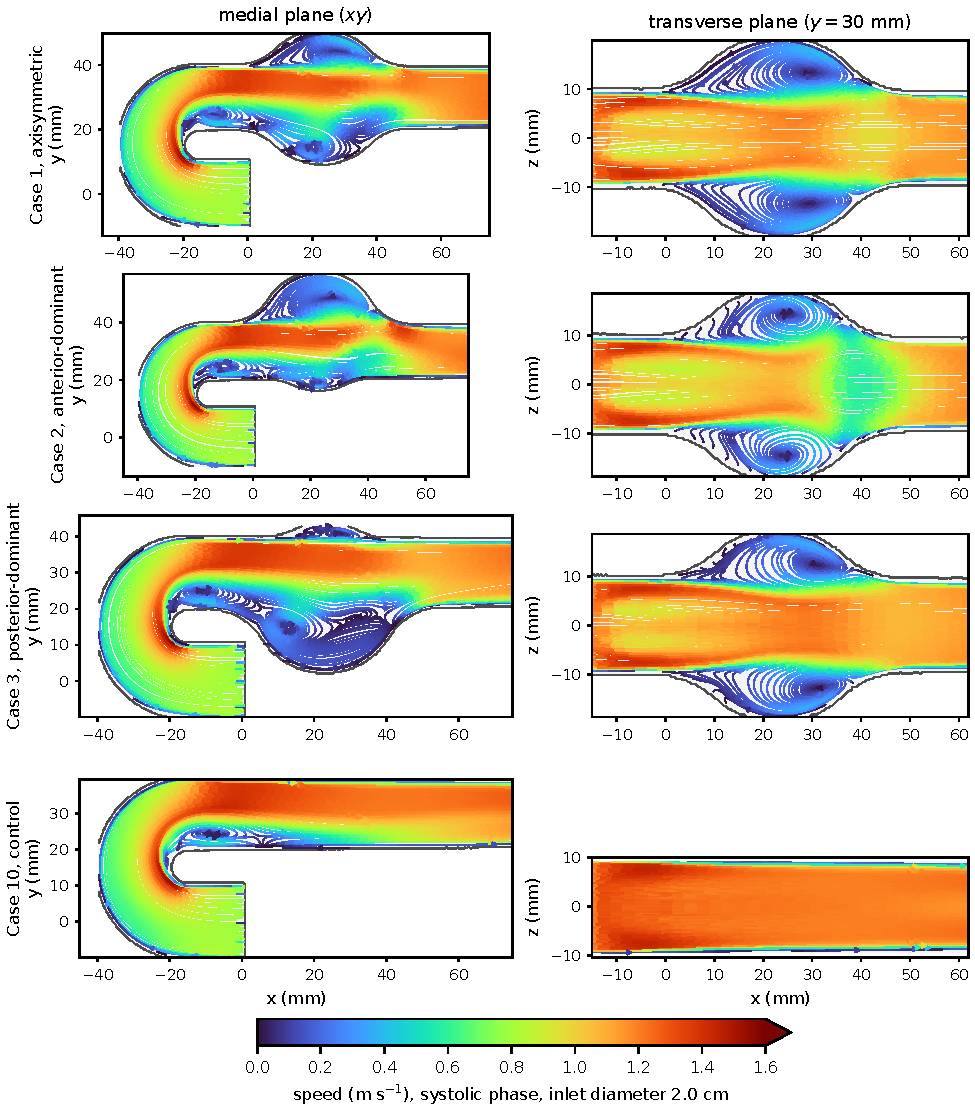
\includegraphics[width=0.92\textwidth]{streamlines_2p0.pdf}
\caption{Streamlines in the systolic phase for the 2.0~cm geometries in the medial plane (left) and the transverse plane (right), colored by in-plane speed on one scale for all geometries. Rows are the axisymmetric, anterior-dominant and posterior-dominant sacs and the control.}
\label{fig:streamlines_2p0}
\end{figure}

\begin{figure}[p]
\centering
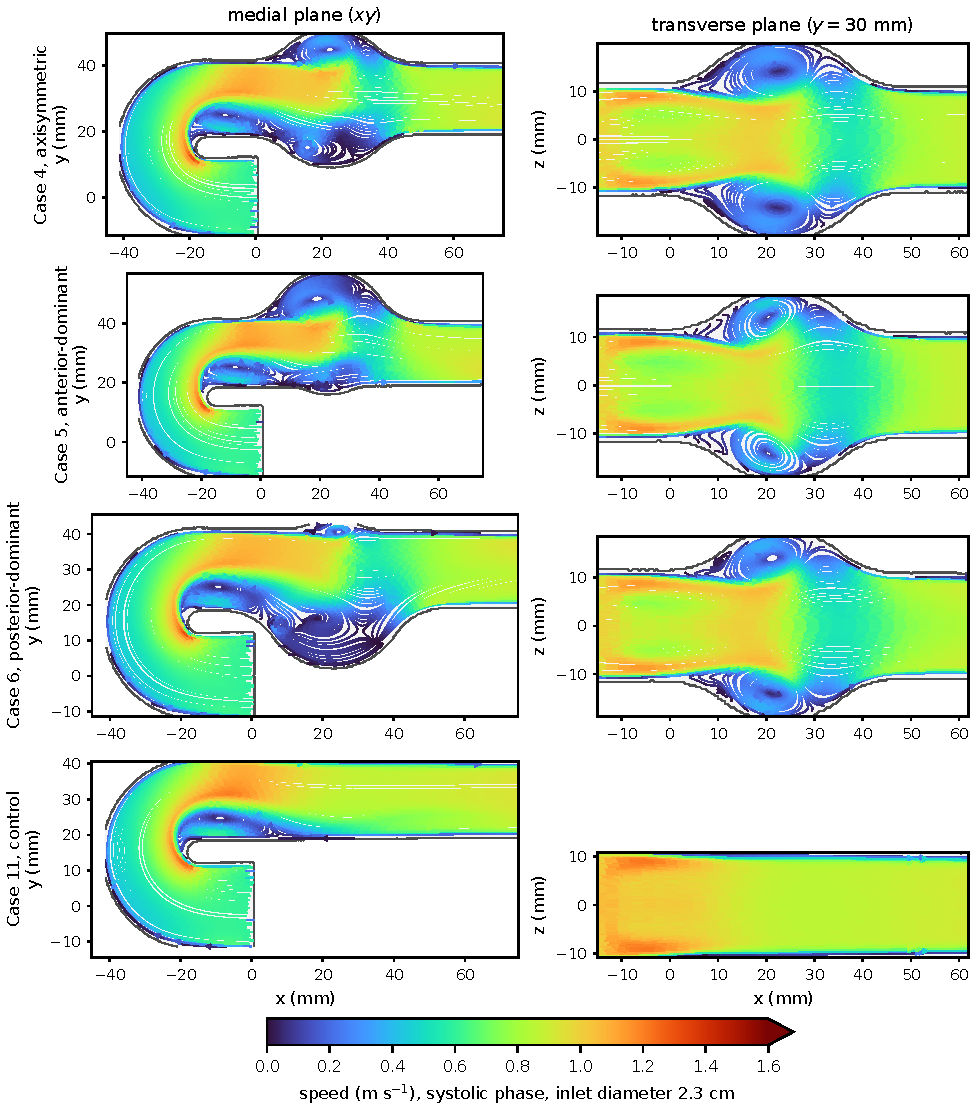
\includegraphics[width=0.92\textwidth]{streamlines_2p3.pdf}
\caption{As Figure~\ref{fig:streamlines_2p0}, for the 2.3~cm geometries.}
\label{fig:streamlines_2p3}
\end{figure}

\begin{figure}[p]
\centering
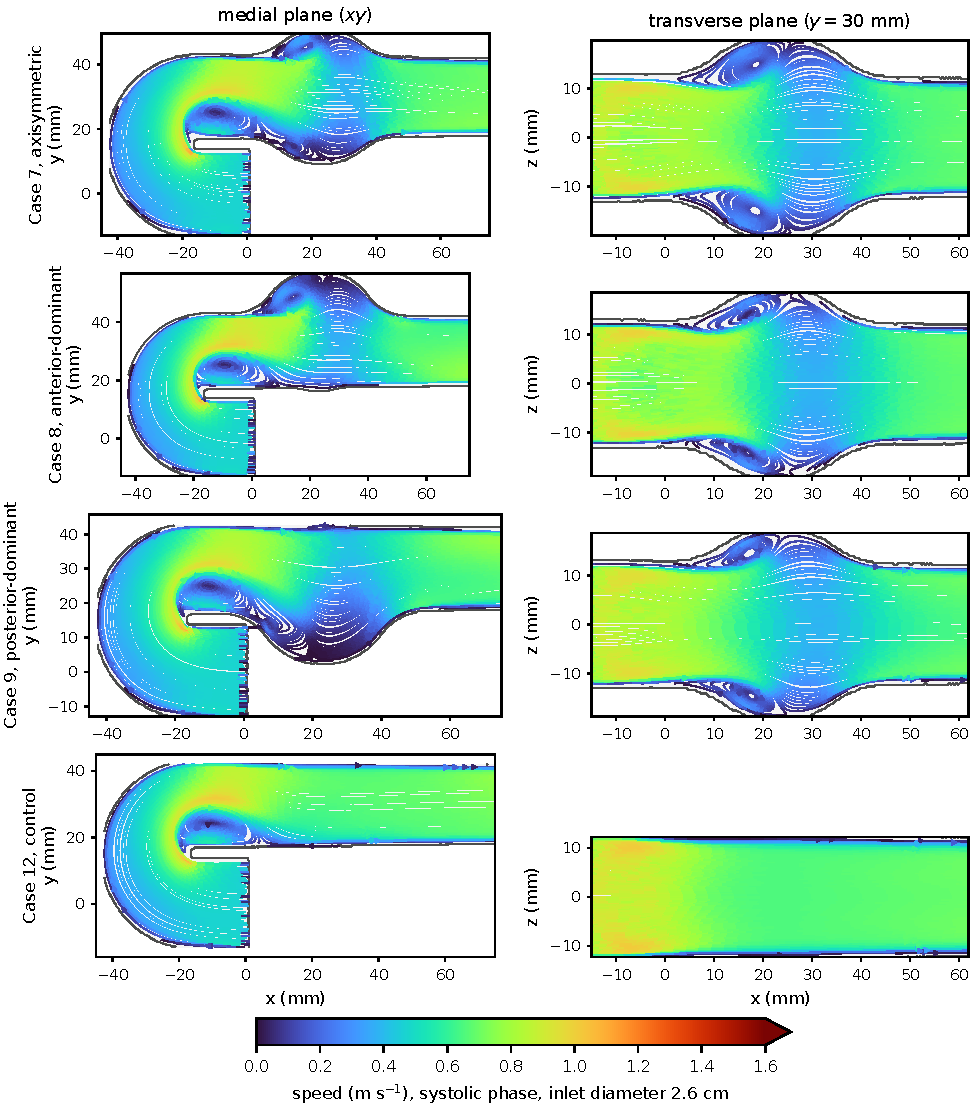
\includegraphics[width=0.92\textwidth]{streamlines_2p6.pdf}
\caption{As Figure~\ref{fig:streamlines_2p0}, for the 2.6~cm geometries.}
\label{fig:streamlines_2p6}
\end{figure}


\subsection{Pressure drop, reversed flow and eddy viscosity}
Table~\ref{tab:cfd_summary} summarizes the common-time flow descriptors for all twelve geometries, and inlet diameter clearly dominates the systolic response. The inlet-to-outlet pressure drop in the systolic phase decreases from \(1261\)--\(1346\,\mathrm{Pa}\) at \(2.0\,\mathrm{cm}\) to \(844\)--\(870\,\mathrm{Pa}\) at \(2.3\,\mathrm{cm}\) and \(528\)--\(561\,\mathrm{Pa}\) at \(2.6\,\mathrm{cm}\), whereas at a fixed diameter the three bulge patterns differ by at most \(7\%\). Relative to the matched control, the dilation adds \(17\)--\(30\%\) to the pressure drop. The fraction of dilation-segment nodes exhibiting reversed axial velocity at systole follows the same ordering, falling from \(50\)--\(54\%\) at \(2.0\,\mathrm{cm}\) to \(38\)--\(40\%\) at \(2.3\,\mathrm{cm}\) and \(24\)--\(28\%\) at \(2.6\,\mathrm{cm}\), against only \(2\)--\(3\%\) in the controls. The mean eddy viscosity within the segment is \(8.6\)--\(9.5\) times the molecular viscosity at \(2.0\,\mathrm{cm}\) but only \(1.6\)--\(2.1\) times at \(2.6\,\mathrm{cm}\). A narrower parent vessel therefore delivers a faster jet into the same \(4.0\,\mathrm{cm}\) sac, producing a larger expansion, a greater fraction of reversed flow, and stronger modeled turbulent mixing. At diastole, by contrast, the pressure drops are only \(1.6\)--\(10.7\,\mathrm{Pa}\), and \(35\)--\(47\%\) of the segment carries reversed flow in every geometry, including the controls, because the slow plateau flow no longer possesses a coherent core.

\input{tables/cfd_summary}

\subsection{Wall shear stress}
Figure~\ref{fig:wss_sys} illustrates the \WSS magnitude over the dilation segment in the systolic phase, unwrapped about the axis of the descending segment. In this representation the anterior wall lies at \(0^\circ\) and the posterior wall at \(\pm180^\circ\), so that the full circumference of the vessel is displayed on a single plane. At systole all aneurysmal cases share a low-shear sac body bounded by high-shear rings at the proximal and distal necks, where the jet enters the sac and reattaches. The median segment \WSS is 1.6--2.8~Pa in the aneurysmal cases against 2.7--5.0~Pa in the controls, whereas the 95th percentile is 1.8--2.4 times that of the matched control (Table~\ref{tab:cfd_summary}). The neck rings weaken with increasing inlet diameter, and the 95th percentile falls from 15--18~Pa at 2.0~cm to 7--8~Pa at 2.6~cm. Asymmetry moves the pattern rather than scaling it. In the anterior-dominant cases the low-shear region is centered on the anterior wall (\(0^\circ\)), whereas in the posterior-dominant cases it is centered on the posterior wall (\(\pm180^\circ\)), so that over the sac body the wall opposite the dominant bulge carries the higher shear. In Case~2 the median sac-body \WSS is 4.5~Pa on the posterior wall against 0.9~Pa on the anterior bulge, and in Case~3 the 95th percentile is 8.4~Pa on the anterior wall against 2.1~Pa on the posterior bulge, with the same ordering in Cases~5, 6 and 9 and nearly equal values in Case~8. This behavior is consistent with the streamlines, which show that the jet crossing the sac impinges on the wall opposite the bulge while the bulge itself is filled by slow recirculating flow. At the distal neck the highest shear lies on the anterior (outer-curvature) side in most cases, irrespective of the bulge direction, because the core leaves the bend along the anterior wall.

Figure~\ref{fig:wss_dia} presents the same \WSS magnitude in the diastolic phase on one color scale per phase. At diastole the effect of asymmetry becomes larger than that of diameter. The median segment \WSS of the asymmetric sacs is 0.45--0.85~Pa, which is 1.8--3.1 times that of the axisymmetric sacs (0.25--0.28~Pa) at every diameter and 2.6--6.8 times that of the controls (0.10--0.17~Pa). On comparison of all cases, the diastolic maps show broad shear over the whole wall of the asymmetric sacs, consistent with a residual vortex that keeps moving along the sac wall during the plateau, whereas the axisymmetric sacs and the controls are close to stagnant. These are instantaneous values at two instants; the cycle-averaged picture is given by the \TAWSS maps in Section~\ref{sec:tawss}.

\begin{figure}[!htb]
\centering
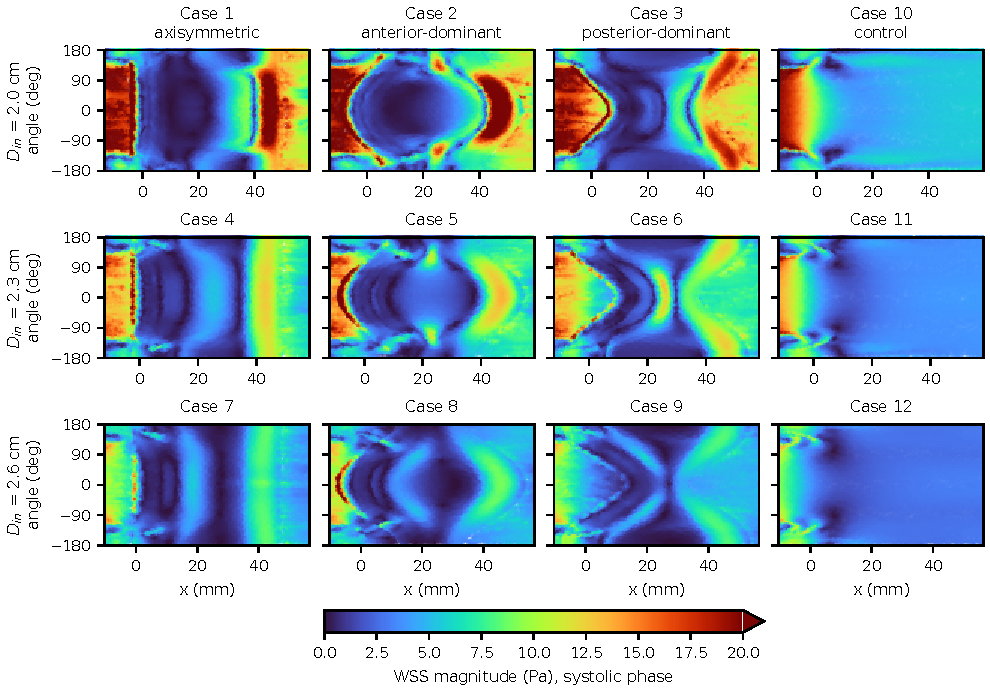
\includegraphics[width=\textwidth]{wss_montage_systole.pdf}
\caption{\WSS magnitude on the dilation segment in the systolic phase, on one color scale saturating at 20~Pa. The wall is unwrapped about the vessel axis, with the anterior wall at \(0^\circ\) and the posterior wall at \(\pm180^\circ\). Rows are inlet diameters and the last column is the matching control. White points are gaps in the exported wall nodes.}
\label{fig:wss_sys}
\end{figure}

\begin{figure}[!htb]
\centering
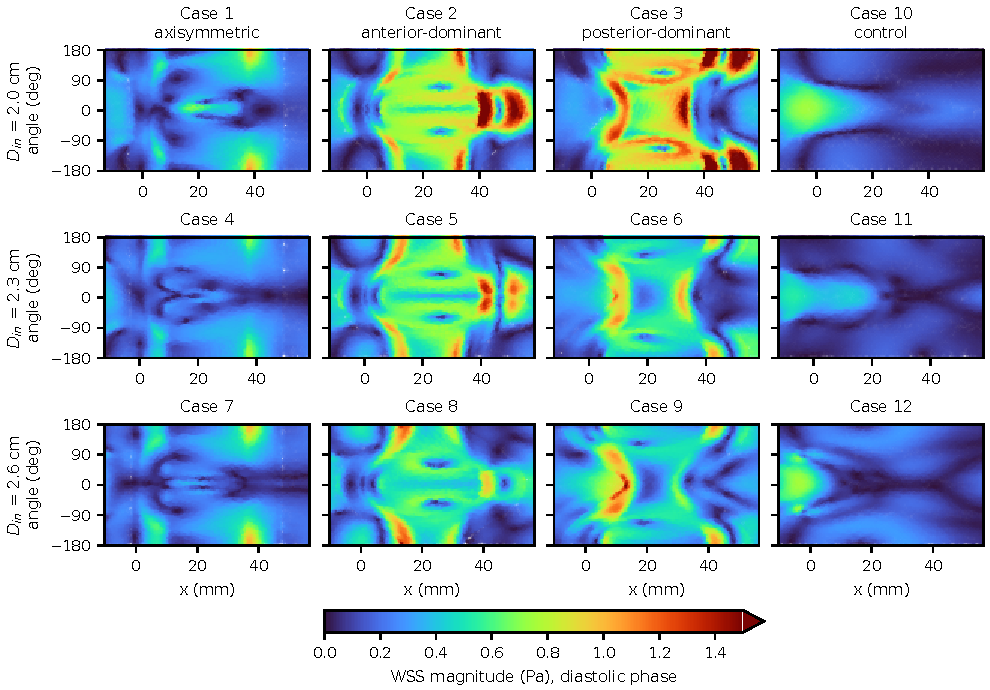
\includegraphics[width=\textwidth]{wss_montage_diastole.pdf}
\caption{As Figure~\ref{fig:wss_sys}, in the diastolic phase, with one color scale saturating at 1.5~Pa.}
\label{fig:wss_dia}
\end{figure}

Figure~\ref{fig:xwss} illustrates the 2D graphics of \WSS for both the medial and transverse planes. Figure~\ref{fig:xwss}(a) represents the \WSS on the anterior wall of the medial plane while Figure~\ref{fig:xwss}(b) shows the \WSS on the posterior wall of the medial plane. Figure~\ref{fig:xwss}(c) presents the \WSS for the transverse plane. Because the aorta bends, a negative value alone does not prove local reverse flow in the curved segment, but along the straight descending segment the negative regions coincide with the recirculation seen in Figures~\ref{fig:streamlines_2p0}--\ref{fig:streamlines_2p6}. On the anterior medial wall and on the transverse wall, \WSS is large and positive at the proximal neck in every case. It becomes negative where the flow detaches on entering the sac, between \(x\approx-4\) and 16~mm on the anterior wall and between 0 and 4~mm on the transverse wall, and it stays negative over the recirculating part of the sac. It returns to positive values, marking reattachment of the core flow, between \(x\approx27\) and 42~mm on the anterior wall and between 26 and 39~mm on the transverse wall, followed by the high positive values of the distal neck. The reattachment point moves upstream as the inlet diameter increases, from 34--42~mm at 2.0~cm to 27--31~mm at 2.6~cm on the anterior wall and from 36--39~mm to 26--27~mm on the transverse wall, so the recirculation region shortens with a wider parent vessel, in line with the reversed-flow fractions of Table~\ref{tab:cfd_summary}. The posterior medial wall differs because \WSS is already negative at the proximal neck in every geometry, the controls included, which identifies this region as the \ICRZ rather than as part of the sac recirculation. The depth of the negative region does not follow the bulge pattern consistently; the most negative value inside the sac, \(-11.3\)~Pa, occurs on the anterior wall of Case~6.

\begin{figure}[!htb]
\centering
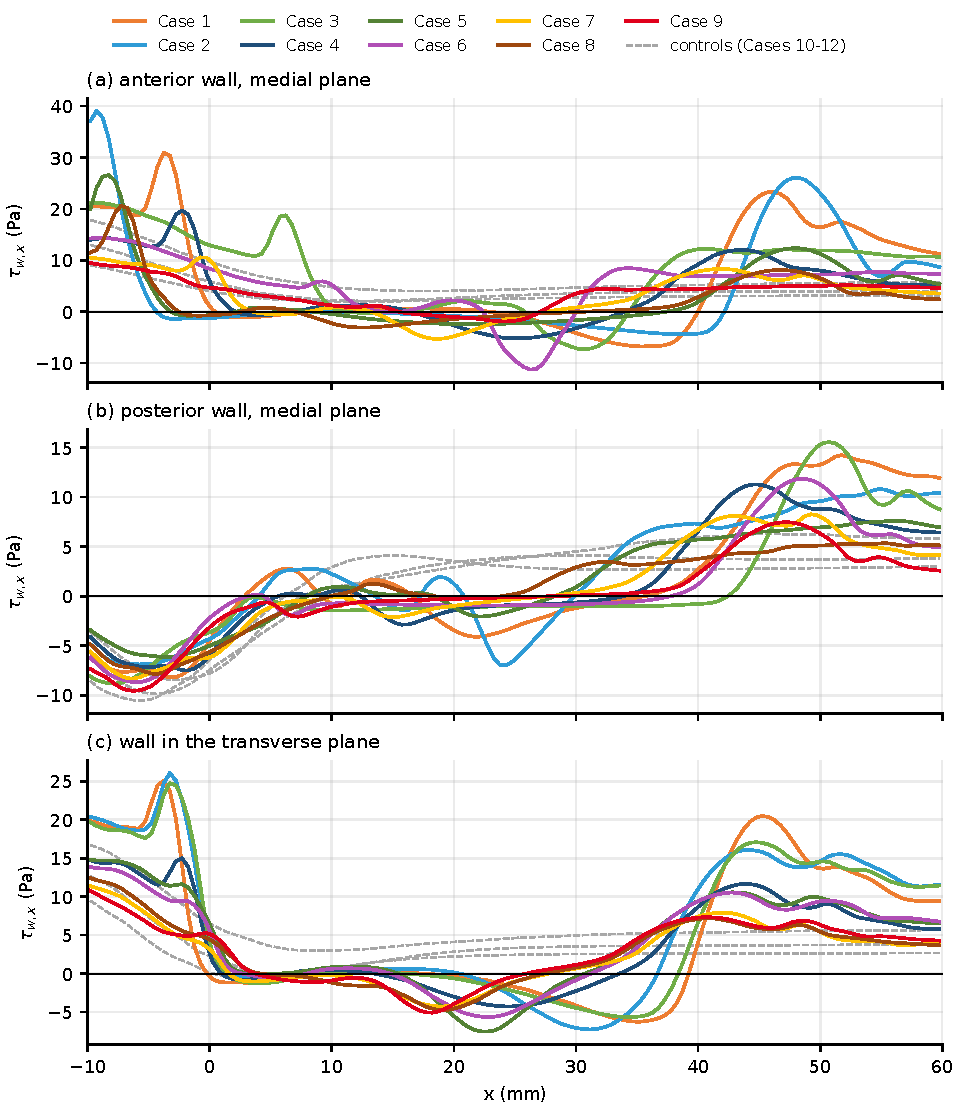
\includegraphics[width=0.85\textwidth]{xwss_lines.pdf}
\caption{2D graphics of \WSS (Pa) in the medial and transverse planes at systolic phase: (a) anterior side of the medial plane, (b) posterior side of the medial plane, and (c) transverse plane.}
\label{fig:xwss}
\end{figure}

\subsection{Time-averaged wall shear stress}
\label{sec:tawss}

The analysis of \TAWSS, as presented in Figure~\ref{fig:tawss} and Table~\ref{tab:tawss}, across twelve idealized geometries revealed several consistent trends. The \TAWSS is shown on the dilation segment of every geometry, unwrapped as in Figure~\ref{fig:wss_sys} and drawn on one logarithmic color scale because the values span two orders of magnitude. Every aneurysmal sac carries a broad region of low \TAWSS. The median over the dilation segment is 0.51--0.83~Pa in the aneurysmal cases against 2.5--4.5~Pa over the same stretch of the controls, while over the sac body the median on either side is 0.23--0.84~Pa. Relative to the matched control, the segment median is lower by a factor of 8.5--8.9 at 2.0~cm, 4.0--4.9 at 2.3~cm and 3.4--3.6 at 2.6~cm, so that the reduction in cycle-averaged shear caused by the dilation is largest for the narrowest parent vessel. Increasing the inlet diameter from 2~cm to 2.6~cm was associated with a progressive reduction in \TAWSS. The high-shear rings at the necks persist in the cycle average, and their strength falls with inlet diameter, the 95th percentile decreasing from 7.6--10.9~Pa at 2.0~cm to 5.5--6.4~Pa at 2.3~cm and 4.1--5.1~Pa at 2.6~cm.

Aneurysm asymmetry had a strong influence on the spatial distribution of \TAWSS. In asymmetric models, the lowest \TAWSS is consistently placed on the dominant bulge. In the anterior-dominant Cases~2, 5 and 8 the sac-body median is 0.34, 0.23 and 0.33~Pa on the anterior wall against 0.52, 0.58 and 0.84~Pa on the posterior wall, whereas in the posterior-dominant Cases~6 and 9 it is 0.24 and 0.28~Pa on the posterior wall against 0.71 and 0.60~Pa on the anterior wall. Case~3 is the exception, with similar values on both sides (0.35 and 0.42~Pa). In the axisymmetric sacs the low-shear region forms circumferential bands with nearly equal anterior and posterior medians. It is also observed that the bulge side is where the instantaneous shear is lowest at systole, so that the dominant bulge is exposed to low shear over the whole cycle rather than at a single instant. This reinforces the need for a multi-parametric hemodynamic assessment that includes both \WSS and \TAWSS to identify rupture-prone \DTAAs. Low \TAWSS, in particular, marks regions of prolonged low shear, which are known to promote thrombus formation~\cite{salman2019biomechanical}, although the present models do not include those processes.

\begin{figure}[!htb]
\centering
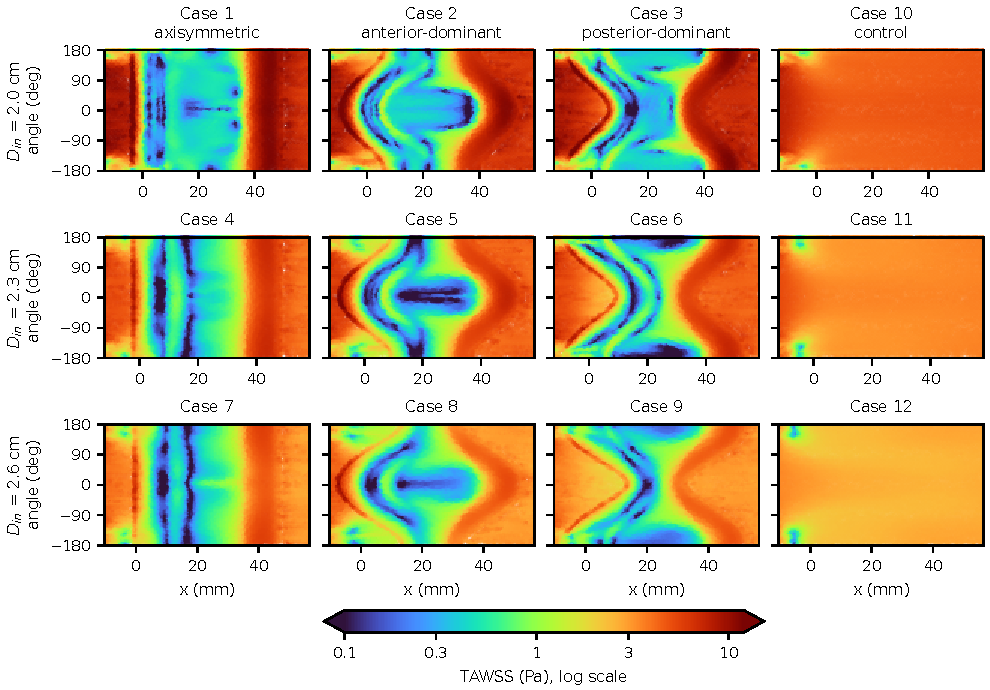
\includegraphics[width=\textwidth]{tawss_montage.pdf}
\caption{\TAWSScap on the dilation segment, unwrapped as in Figure~\ref{fig:wss_sys}, on one logarithmic color scale. Rows are inlet diameters and the last column is the matching control.}
\label{fig:tawss}
\end{figure}

\input{tables/tawss_summary}

\FloatBarrier

\subsection{Structural wall stress}
\label{sec:structural}

It is widely recognized that aneurysm rupture risk is associated with maximum diameter; however, this relationship is not absolute. Darling et al.~\cite{darling1977autopsy} observed that some large aneurysms do not rupture, whereas smaller ones do, indicating that additional factors such as aneurysm geometry and asymmetry play a critical role. Aneurysm rupture occurs when the mechanical load exceeds the tissue strength of the arterial wall, and understanding this mechanical mechanism is essential for assessing rupture risk in \DTAA. Our results indicate that aneurysm shape and inlet diameter markedly change the modeled wall-stress distribution. Previous studies, including those by Dobrin~\cite{dobrin1989pathophysiology}, have applied Laplace's law to estimate wall stress. However, Laplace's law predicts the greatest wall stress at the maximum bulge of the aneurysm sac, which is not consistent with the biomechanical behavior observed in aneurysmal geometries. As demonstrated in the present study, the stress distribution within the aneurysm wall is governed by asymmetry and geometric features.

Figure~\ref{fig:mps} presents the \MPS on the inner surface of the wall over the dilation segment, unwrapped as in Figure~\ref{fig:wss_sys}, and Table~\ref{tab:mps} summarizes it. In every aneurysmal case the \MPS is highest in circumferential bands at the necks, where the wall curvature changes sign, with 95th percentiles of 101--113~kPa over the necks, and lowest over the crown of the sac, where the medians are 55--80~kPa. This pattern is consistent with the findings of Vorp et al.~\cite{vorp1998mechanical}. A clear distinction was observed between axisymmetric and asymmetric cases. In the axisymmetric models, the stress was elevated at the proximal regions but lower at the midsection of the aneurysm sac, with similar behavior on both anterior and posterior sides; the anterior and posterior sac-body medians are equal to within 1~kPa. In contrast, the asymmetric models exhibited higher stress on the side opposite to the dominant bulge. The sac-body median on the posterior wall of the anterior-dominant Cases~2, 5 and 8 is 69.2, 73.6 and 78.1~kPa against 55.9, 55.0 and 61.8~kPa on the anterior bulge, and the anterior wall of the posterior-dominant Cases~3, 6 and 9 carries 68.3, 72.9 and 80.3~kPa against 55.8, 55.3 and 57.2~kPa on the posterior bulge. The opposite-side value increases with inlet diameter, as does the segment median of the controls (52.5, 58.4 and 65.1~kPa), because the loaded radius grows with the parent vessel.

In contrast, the healthy cases (10--12) exhibited relatively uniform wall stress distributions, with 95th percentiles within 3~kPa of their medians and only mild elevations at the bend. Compared to the diseased cases, where stress varied non-uniformly due to the presence of the aneurysm, the healthy aortas showed more consistent stress profiles. Assuming uniform wall strength, these results indicate that the side opposite to the dominant bulge is at a higher risk of rupture compared to the other side. Among the six asymmetric cases, the highest \MPS was observed in Case~9 on the anterior side, so that, if the wall strength were the same on both sides, this site would carry the highest modeled stress of all sides and cases. With a uniform 2~mm wall, literature material parameters, fixed ends and a quasi-static coupling whose step settings were not retained, the stress magnitudes indicate where the modeled wall is most loaded rather than where it would fail, since failure also depends on the unknown local wall strength.

\begin{figure}[!htb]
\centering
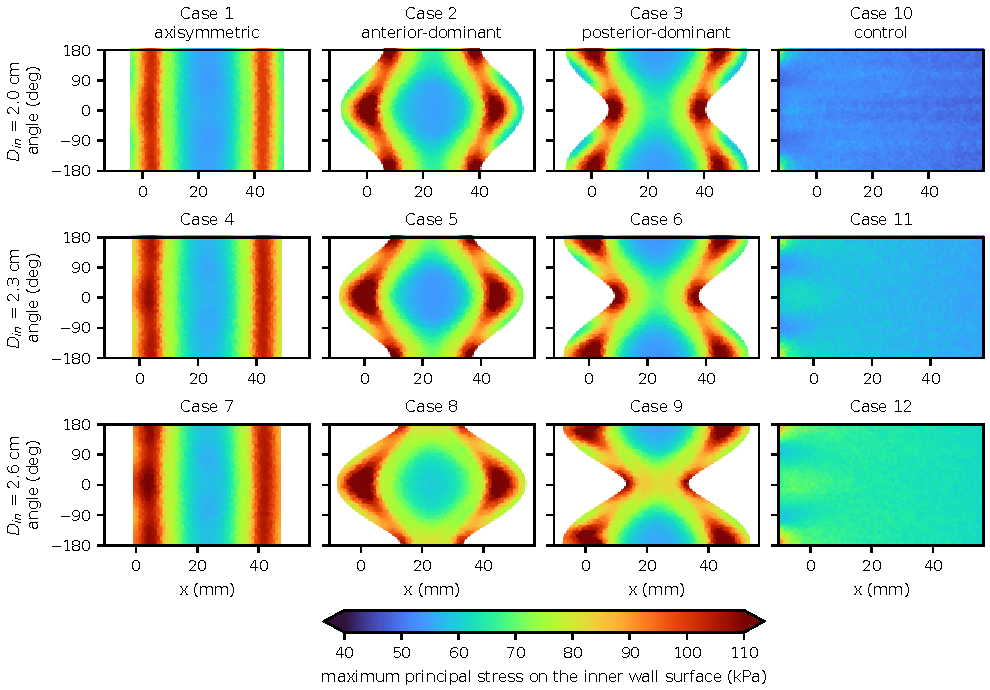
\includegraphics[width=\textwidth]{mps_montage.pdf}
\caption{\MPScap on the inner wall surface of the dilation segment, unwrapped as in Figure~\ref{fig:wss_sys}, on one color scale. Rows are inlet diameters and the last column is the matching control.}
\label{fig:mps}
\end{figure}

\input{tables/mps_summary}

\FloatBarrier

\subsection{Plane-wise flow summaries}
\label{sec:planes}

In addition to the wall-based hemodynamic and biomechanical indices, a plane-wise cross-sectional analysis was performed to quantify the spatial variation of flow features along the aorta. Velocity and \TKE were evaluated at selected axial planes to identify the regions where aneurysm morphology most strongly altered the flow field. This approach allows the three-dimensional flow disturbance to be reduced into comparable regional quantities from the proximal to distal sections of the vessel.

The locations of the eight planes are shown in Figure~\ref{fig:diagram} and the details of aortic diameter are available in Table~\ref{tab:diameter}. All models incorporated a taper ratio of 0.8 from inlet to outlet, a physiologically important feature that gradually reduces the vessel diameter distally, thereby maintaining flow momentum and regulating perfusion to downstream vessels. Figure~\ref{fig:planes} shows the plane-averaged speed and \TKE of every case from the retained slice summaries, and Table~\ref{tab:plane_cfd} gives the medians of the aneurysmal and control groups. The taper is visible in every model, with the speed at D7 and D8 above that at D1--D3 because the lumen narrows toward the outlet. This tapering-induced acceleration is essential for maintaining adequate perfusion pressure that ensures sufficient blood flow to downstream vascular beds. Indeed, studies have shown that flow velocity increases while vessel diameter decreases~\cite{kahveci2015numerical}. In the aneurysmal cases the speed falls sharply across the sac to 0.10--0.16~m~s$^{-1}$ at D5, where the lumen diameter is 4.0~cm whatever the inlet diameter, against a median of 0.193~m~s$^{-1}$ in the controls, and it recovers by D7. This is a direct consequence of the local dilation, where the increased cross-sectional area reduces flow velocity to conserve mass.

In contrast to velocity, the modeled $k$ as shown in Figure~\ref{fig:planes} rises through the sac, peaks at D5 at about twice the control value, remains elevated at D6 and D7, where the jet reattaches and the recirculation of the distal sac develops, and returns to the control level by D8. At plane~5 (the maximum diameter of the bulge, the center of the aneurysm sac), strong flow separation and recirculation zones produce high $k$. At plane~6 (distal sac) and plane~7 (post-aneurysm), $k$ remains elevated, implying that the disturbed flow persists downstream of the aneurysm sac. This pattern is consistent with the fact that recirculation zones predominantly appear on the distal side of the aneurysm, where the flow jet impinges and vortices develop~\cite{yu2000steady}. Conversely, at D4, the proximal neck, the aneurysmal and control values still overlap, so the turbulent disturbance is generated inside the sac rather than at its entrance, and it decays within about one sac length downstream. Thus, $k$ only rises sharply once the flow reaches the central and distal portions of the sac, where recirculation becomes fully established. By plane~8 (near the outlet), the $k$ has returned to the control level, demonstrating that the turbulence has largely dissipated before reaching the distal boundary. The asymmetric sacs reach higher $k$ at D5 than the axisymmetric ones at every diameter.

Overall, the plane-wise analysis confirms that the aneurysm-induced flow disturbance is highly localized rather than uniformly distributed along the entire aorta. The velocity results identified the strongest reduction at plane~5, corresponding to the maximum aneurysm diameter, whereas the $k$ results showed that disturbed and vortical flow persists from the aneurysm center to the distal sac and post-aneurysm region. Thus, the plane-based quantities provide complementary information to the wall-based indices. While \WSS and \TAWSS describe near-wall hemodynamic loading and \MPS describes structural wall stress, the plane-wise velocity and $k$ analysis captures the intraluminal flow disturbance and its downstream propagation. Therefore, the plane-wise analysis provides quantitative evidence that the maximum aneurysm diameter primarily reduces local velocity, whereas aneurysm morphology and sac expansion generate elevated \TKE over a broader downstream region.

\begin{figure}[!htb]
\centering
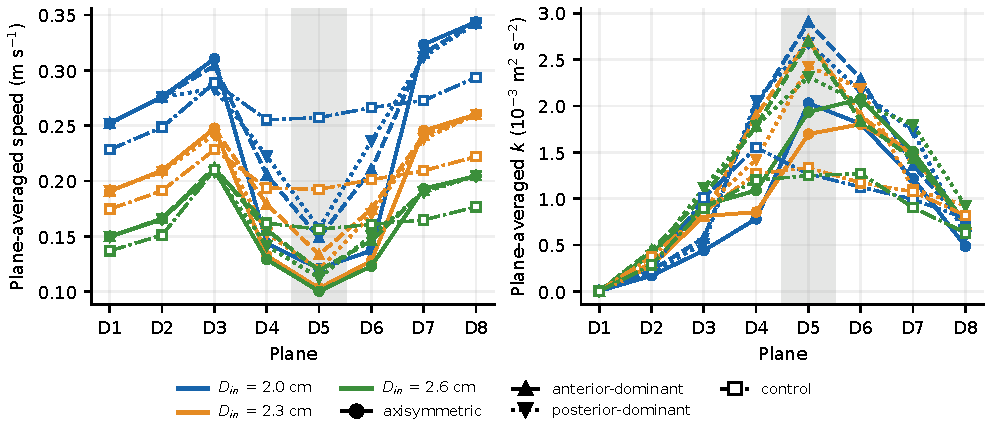
\includegraphics[width=\textwidth]{plane_profiles.pdf}
\caption{Plane-averaged speed (left) and \TKE per unit mass (right) at D1--D8 for all twelve geometries. Color gives the inlet diameter, and line style and marker the morphology; controls are dash-dot with open squares. The band marks the sac center (D5).}
\label{fig:planes}
\end{figure}

\input{tables/plane_cfd}

\section{Reconstruction results}
\label{sec:reconstruction_results}
\subsection{Checks on the complete \texorpdfstring{\CFD}{CFD} fields}
\label{sec:reference_results}
Before any fitting, the complete \CFD fields of the nine aneurysmal cases were used to check Eq.~\eqref{eq:momentum} and to measure the post-processing floors. With 40-neighbor least-squares gradients, the unsteady form with the \CFD eddy viscosity and without a $2\rho k/3$ term gave the smallest momentum residual in every case and phase, at 0.03--0.17 of the convective term in the bulk of the lumen. Omitting the time derivative raised the residual to 0.18--0.30 of convection at systole, and to 0.45--0.56 inside the sac, and to 0.49--0.73 at diastole, and adding the $2\rho k/3$ term made the residual larger. A quasi-steady momentum residual is therefore not consistent with these transient fields, particularly inside the sac.

Table~\ref{tab:reference_floor} gives the floors obtained by passing the complete \CFD velocity through the shared post-processing. Integrating the \CFD's own pressure gradient reproduces the \CFD pressure to 0.5--0.9\%, so the integration itself is accurate, and the remaining floor comes from the momentum terms. With the unsteady form and oracle $\mu_t$ the pressure floor is 1.6--2.3\% at systole, except for Case~2, whose forward window gives 7.1\%, and 2.2--4.1\% at diastole. Information matters differently in the two phases. At systole the molecular form is almost as good as the oracle for the 2.3 and 2.6~cm cases (1.8--2.7\%) but not for the 2.0~cm cases (4.9--11.3\%), in line with their larger eddy viscosity (Table~\ref{tab:cfd_summary}). At diastole removing either the time term or the eddy viscosity degrades the floor substantially, to 3.9--10.3\% and 9.0--19.3\%, respectively. The \WSS floor depends strongly on the distance $h$ in Eq.~\eqref{eq:wss_estimate}. At systole it is 0.07--0.09 at $h=0.1$~mm but 0.14--0.27 at the prespecified $h=0.25$~mm, because the systolic velocity profile is no longer close to quadratic over the $2h=0.5$~mm stencil, whereas at diastole it is 0.04--0.06 at either distance.

\input{tables/reference_floor}

\subsection{Momentum-constrained \texorpdfstring{\PINNs}{PINNs} on the development geometries}
\label{sec:pilot_results}
In the development cases, every neural field reconstructed the hidden velocity three to four times more accurately than \RBF (relative errors 0.037--0.052 versus 0.13--0.16 at systole) and five times more accurately than linear interpolation. However, the prespecified criterion of the development test failed on both endpoints (Table~\ref{tab:pilot}). The momentum arms were trained with a blood density of 1060~kg~m$^{-3}$ in the scaling of their residual before the density was corrected to 1050~kg~m$^{-3}$; all reported scores use the corrected value, and the 1\% difference in the residual scaling does not affect the conclusions drawn from them. The gate scored the momentum \PINNs by their own pressure output and automatic-differentiation \WSS, the direct route that a \PINN offers, and the other methods by shared post-processing, so the comparison changes both the fitting and the pressure route. The unsteady \PINN's own pressure output had errors of 0.43--0.53 at systole and 0.56--1.05 at diastole, and the steady \PINN's 0.51--0.90, whereas the continuity field passed through the shared integration reached 0.023--0.049. The \PINN's automatic-differentiation \WSS (0.40--0.45 at systole) was also worse than the pipeline \WSS of the continuity field (0.35--0.37).

Because the gate changed both the fitting and the pressure route, we also passed the velocity of every momentum \PINN through the shared post-processing (Table~\ref{tab:pilot_pipeline}). In the prespecified unsteady form the unsteady \PINN's velocity still gave pressure errors of 0.37--0.48 at systole and 0.58--1.11 at diastole, against 0.023--0.049 for the continuity field, because that form uses the difference between the field's two snapshots. Dropping the time term reduced the error to 0.037--0.089, still above the continuity field. The \PINN's momentum residual was an order of magnitude smaller than that of the continuity field (0.2 against 2.5 in scaled units), so the network satisfied the momentum balance by adjusting a time derivative that was constrained only at the observed nodes of two snapshots 5--10~ms apart. With so little temporal information, $\partial_t\mathbf u$ and the pressure act as slack variables in a soft momentum penalty rather than as information. The steady \PINN, whose loss does not contain a time derivative, came close to the continuity field only in the systolic window of Case~1 (0.029 against 0.025). For \WSS the shared estimate gave similar errors for all fields at systole (0.34--0.40), and the momentum \PINNs gave lower errors in the diastolic Case~9 window (0.11--0.12 against 0.22). Adding the momentum balance to the loss therefore did not improve the velocity used for pressure, although it helped \WSS in one diastolic window. The confirmation study therefore evaluated the continuity field with physics applied after fitting, as specified in Section~\ref{sec:protocol}.


\input{tables/pilot_endpoints}
\input{tables/pilot_pipeline}

\subsection{Confirmation on seven held-out geometries}
\label{sec:confirmation}
At the primary 2.5~mm spacing the continuity field followed by the shared post-processing had lower pressure error than \RBF with the same post-processing in all 14 case--phase units, with a median ratio of 0.458, and lower aneurysm-zone \WSS error in all 14 units, with a median ratio of 0.508 (Table~\ref{tab:recon_summary}, Figure~\ref{fig:confirmation}). Both prespecified hypotheses were met, and the velocity guardrail held in every unit, with hidden-velocity errors of 0.033--0.050 against 0.113--0.169 for \RBF. At the level of individual draws the \WSS advantage held in 42 of 42 comparisons, whereas the pressure advantage held in 39 of 42. The prespecified decision rule was the count of units, and no significance test was planned. For reference, a two-sided sign test on the draw-level comparisons gives $p<10^{-8}$ for both quantities, although draws within a unit share a geometry and are not independent. The three adverse pressure draws were all diastolic, in Case~4 (ratio 1.05), Case~7 (1.40) and Case~8 (1.75), and the case-wise tables in Appendix~\ref{app:casewise} show that the diastolic pressure error of the neural field varies between draws by up to 0.085, several times more than \RBF's.

\input{tables/reconstruction_summary}

\begin{figure}[!htb]
\centering
\begin{minipage}{0.48\textwidth}
\centering
\begin{tikzpicture}
\begin{axis}[width=0.90\linewidth,height=5.8cm,xmin=0,xmax=0.20,ymin=0,ymax=0.20,
 xlabel={\RBF pressure error},ylabel={Continuity-field pressure error},
 tick label style={font=\scriptsize},label style={font=\small},grid=major,
 legend style={font=\scriptsize,at={(0.03,0.97)},anchor=north west,draw=none}]
\addplot[black,dashed,forget plot] coordinates {(0,0) (0.20,0.20)};
\addplot[only marks,mark=*,blue] table[x=rbf,y=field]{figures/generated/confirm_p_sys.dat};
\addlegendentry{Systole}
\addplot[only marks,mark=square*,red] table[x=rbf,y=field]{figures/generated/confirm_p_dia.dat};
\addlegendentry{Diastole}
\end{axis}
\end{tikzpicture}
\end{minipage}
\hfill
\begin{minipage}{0.48\textwidth}
\centering
\begin{tikzpicture}
\begin{axis}[width=0.90\linewidth,height=5.8cm,xmin=0,xmax=0.75,ymin=0,ymax=0.75,
 xlabel={\RBF \WSS error},ylabel={Continuity-field \WSS error},
 tick label style={font=\scriptsize},label style={font=\small},grid=major]
\addplot[black,dashed,forget plot] coordinates {(0,0) (0.75,0.75)};
\addplot[only marks,mark=*,blue] table[x=rbf,y=field]{figures/generated/confirm_wss_sys.dat};
\addplot[only marks,mark=square*,red] table[x=rbf,y=field]{figures/generated/confirm_wss_dia.dat};
\end{axis}
\end{tikzpicture}
\end{minipage}
\caption{Case-wise confirmation errors for pressure (left, unsteady form with oracle $\mu_t$) and aneurysm-zone \WSS magnitude (right, $h=0.25$~mm) at 2.5~mm. Each point is one case--phase unit averaged over three paired draws; points below the diagonal favor the continuity field. Both pipelines receive the same oracle eddy viscosity.}
\label{fig:confirmation}
\end{figure}

The phases differ in how close the reconstruction comes to its floor. At systole the median pressure error of the continuity field, 0.023, is close to the floor of 0.019, so the reconstructed velocity is good enough that the post-processing, not the reconstruction, sets most of the pressure error. At diastole the median error of 0.094 is two and a half times the floor of 0.037, and the advantage over \RBF (0.132) is small in Cases~7 and 8 (0.155 against 0.171 and 0.101 against 0.104). The median systolic \WSS error of 0.356 lies well above its floor of 0.191, and the diastolic 0.163 lies well above 0.042, so for \WSS the reconstruction remains the limiting step.

\subsection{Local errors and field maps}
\label{sec:local}
Global relative errors can hide local failures, so Table~\ref{tab:local_metrics} and Figures~\ref{fig:velocity_maps}--\ref{fig:field_maps_adverse} report local measures. The 95th percentile of the pointwise velocity error magnitude in systole is 0.057~m~s$^{-1}$ for the continuity field and 0.20~m~s$^{-1}$ for \RBF, against peak speeds of about 1.0--1.6~m~s$^{-1}$, and within the sac the relative velocity error is 0.075 against 0.185. The largest pointwise velocity errors of the continuity field lie in the thin shear layer where the flow separates at the bend exit (Figure~\ref{fig:velocity_maps}).

\input{tables/local_metrics}

\begin{figure}[H]
\centering
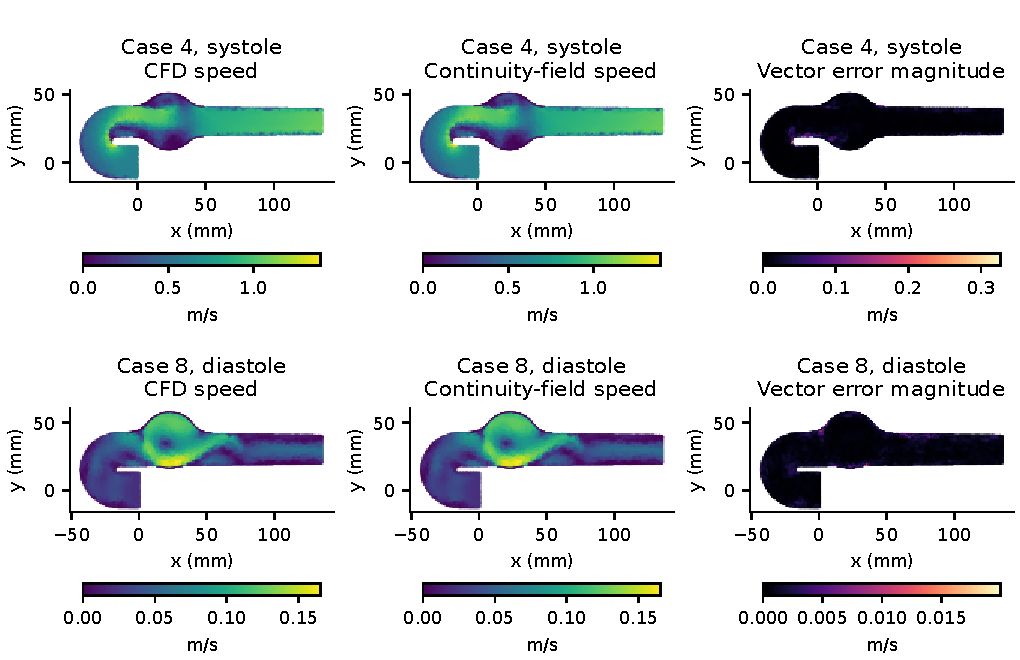
\includegraphics[width=0.90\textwidth]{hidden_velocity_examples.pdf}
\caption{Hidden-node speed on the mid-plane ($|z-z_{\rm mid}|<0.35$~mm) for Case~4 at systole and Case~8 at diastole (draw 0, 2.5~mm). Left, \CFD; center, continuity field; right, magnitude of the vector error. Only unobserved nodes are shown.}
\label{fig:velocity_maps}
\end{figure}

The 99th percentile of aneurysm-zone \WSS is recovered to 0.92 of the \CFD value at systole and 0.90 at diastole, whereas \RBF recovers only 0.52 and 0.61 of it, so \RBF's \WSS error consists mostly of flattened peaks. The Pearson correlation between reconstructed and \CFD \WSS magnitude is 0.92 at systole and 0.94 at diastole for the continuity field, against 0.87 and 0.79 for \RBF, and the \WSS vector errors are 0.38 and 0.20 against 0.62 and 0.42. The systolic pressure drop, which ranges from 413 to 1063~Pa across the cases, is recovered with a median absolute error of 6~Pa against 31~Pa for \RBF. At diastole the median drop errors of 0.48 and 0.67~Pa are comparable to the drops themselves (0.4--5.8~Pa), so neither method recovers the diastolic drop reliably, even though the relative error over the whole pressure field is modest.

The two kinds of error also differ in form. In the median systolic unit (Figure~\ref{fig:field_maps}) the continuity field reproduces the \WSS rings at both necks, while \RBF smears them and underestimates their peaks.

\begin{figure}[H]
\centering
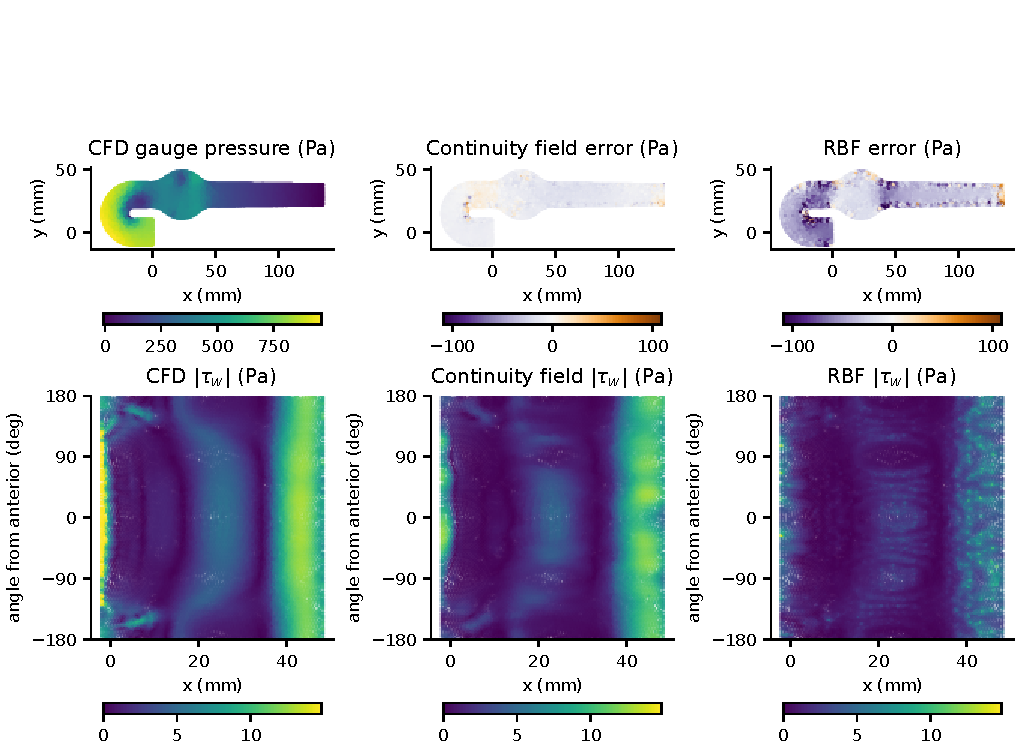
\includegraphics[width=0.95\textwidth]{field_maps_c04_t1780.pdf}
\caption{Case~4 at systole (draw 0, 2.5~mm), close to the median result. Top, \CFD mid-plane pressure and the pressure errors of the continuity field and \RBF. Bottom, aneurysm-zone \WSS unwrapped about the vessel axis. Relative errors are 0.024 and 0.100 for pressure and 0.32 and 0.60 for \WSS.}
\label{fig:field_maps}
\end{figure}

In the adverse diastolic unit (Figure~\ref{fig:field_maps_adverse}), the continuity field's pressure error is a smooth offset of about 1~Pa that accumulates along the vessel, which points to a small bias in the integrated pressure gradient such as the two-snapshot acceleration, while \RBF's pressure errors are concentrated near the sac necks.

\begin{figure}[H]
\centering
\IfFileExists{figures/generated/field_maps_c07_t2400.pdf}{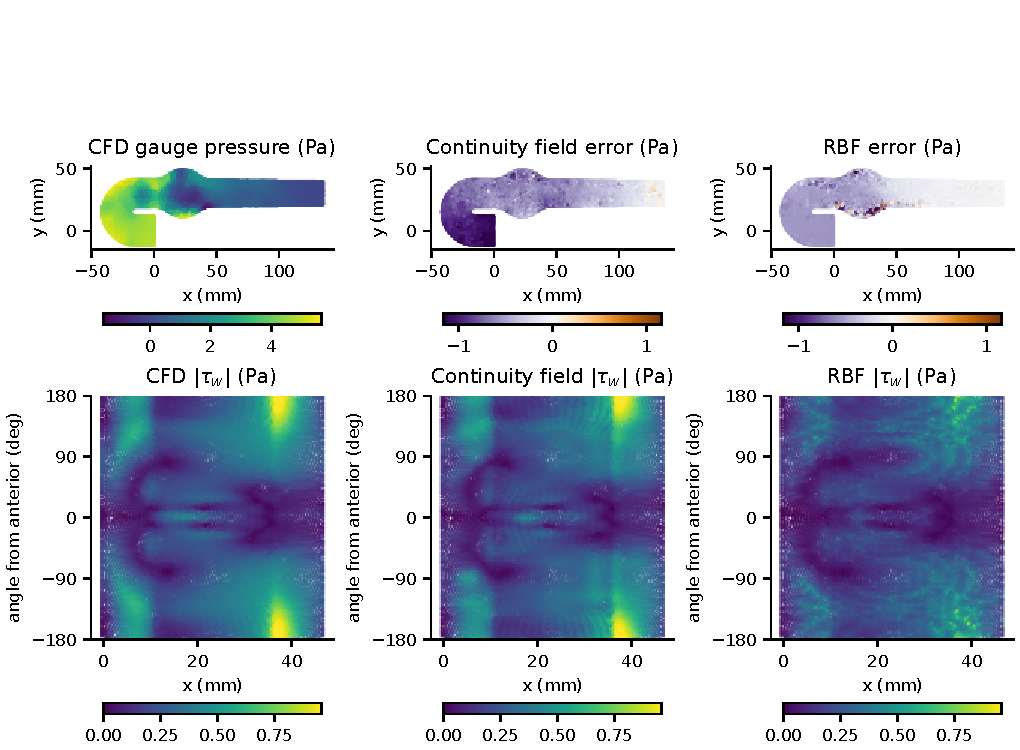
\includegraphics[width=0.95\textwidth]{field_maps_c07_t2400.pdf}}{\fbox{Case 7 diastolic maps pending}}
\caption{As Figure~\ref{fig:field_maps}, for the adverse unit Case~7 at diastole. Relative errors are 0.25 and 0.18 for pressure and 0.14 and 0.33 for \WSS. The \CFD pressure varies by only a few pascals, so errors of about 1~Pa dominate.}
\label{fig:field_maps_adverse}
\end{figure}

The \WSS calculated by automatic differentiation of the continuity field itself was worse than the finite-distance estimate from the same field (median 0.55 against 0.36 in systole and 0.27 against 0.16 in diastole). The soft no-slip penalty fixes the velocity at the wall but leaves its wall-normal gradient poorly determined, so the network's analytic derivative should not be read as \WSS. The finite-distance estimate is also sensitive to $h$. Evaluated at 0.1~mm instead of 0.25~mm, the continuity field's median systolic \WSS error falls from 0.356 to 0.326, and at 0.5~mm it rises to 0.476. We keep the prespecified distance because choosing $h$ with knowledge of the \WSS target would be information that a deployment does not have.

\subsection{Contribution of the continuity penalty and sampling density}
\label{sec:ablation}
Figure~\ref{fig:budget} separates the effect of the continuity penalty from that of the neural representation. At 2.5~mm, the data field without an interior PDE penalty is close to the continuity field, with median velocity errors of 0.052 and 0.039 versus 0.044 and 0.038, and is slightly better on two endpoints, diastolic pressure (0.063 versus 0.094) and systolic \WSS (0.333 versus 0.356). At the densest spacing of 1.5~mm the data field is better on every endpoint except systolic pressure. Only at the sparsest spacing of 4.0~mm, where the observations cover 0.34--0.37\% of the nodes, does the continuity penalty help consistently, reducing the median hidden-velocity error from 0.125 to 0.077 at systole and from 0.105 to 0.077 at diastole, the systolic pressure error from 0.072 to 0.052 and the diastolic \WSS error from 0.371 to 0.316. The main advantage over \RBF therefore comes from fitting one smooth space-time representation to both snapshots, and continuity becomes useful when the data alone no longer determine the field.

The advantage of both neural fields over \RBF grows as the observations become sparser. The median systolic pressure errors at 1.5, 2.5 and 4.0~mm are 0.024, 0.023 and 0.052 for the continuity field versus 0.029, 0.079 and 0.178 for \RBF, and the median systolic \WSS errors are 0.30, 0.36 and 0.48 versus 0.49, 0.61 and 0.68. At diastole and 4.0~mm the continuity field's pressure error is 0.096 versus 0.318 for \RBF. Only one draw was performed at 1.5 and 4.0~mm, so these values describe a trend rather than an uncertainty interval.

\begin{figure}[H]
\centering
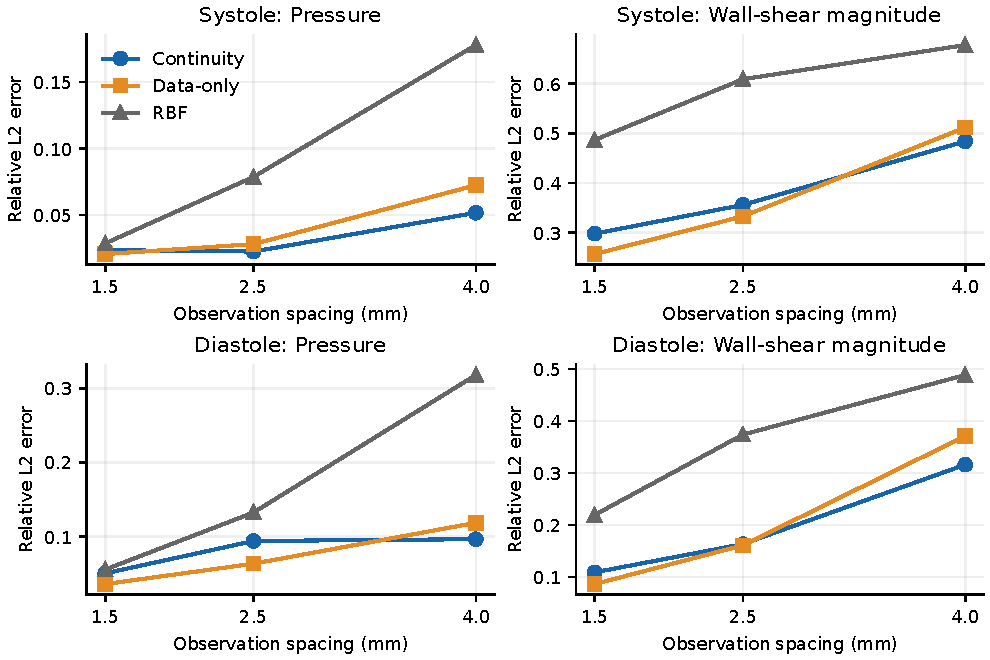
\includegraphics[width=0.92\textwidth]{observation_budget.pdf}
\caption{Median pressure (unsteady form with oracle $\mu_t$) and aneurysm-zone \WSS errors over Cases~2--8 against observation spacing. The 2.5~mm values average three draws per case; 1.5 and 4.0~mm use one draw.}
\label{fig:budget}
\end{figure}

Figure~\ref{fig:pressure_information} asks two separate questions about pressure recovery, namely whether to retain the local acceleration term and whether to supply the \CFD eddy viscosity. Here, steady and unsteady refer to the pressure calculation applied after reconstruction, not to separately trained neural fields. In the seven confirmation geometries, the systolic median improves when the time term is retained and changes little when the eddy viscosity is removed. The unsteady form gives a median error of 0.023 against 0.034 for the steady form, close to the floors of 0.019 and 0.036, and dropping $\mu_t$ changes 0.023 to 0.027. At diastole the eddy viscosity is essential, since removing it more than doubles the continuity field's error, from 0.094 to 0.207, and raises the floor from 0.037 to 0.154. The time term behaves differently for the reconstruction and for the complete \CFD field at diastole. The floor favors the unsteady form (0.037 against 0.065), but the continuity field does better with the steady form (0.072 against 0.094), because the 10~ms finite difference of two reconstructed diastolic fields, whose speeds are about one tenth of the systolic ones, amplifies small reconstruction errors. Diastolic pressure recovery in this setting therefore needs both an estimate of the eddy viscosity and a more accurate acceleration than two sparse snapshots provide.

\begin{figure}[H]
\centering
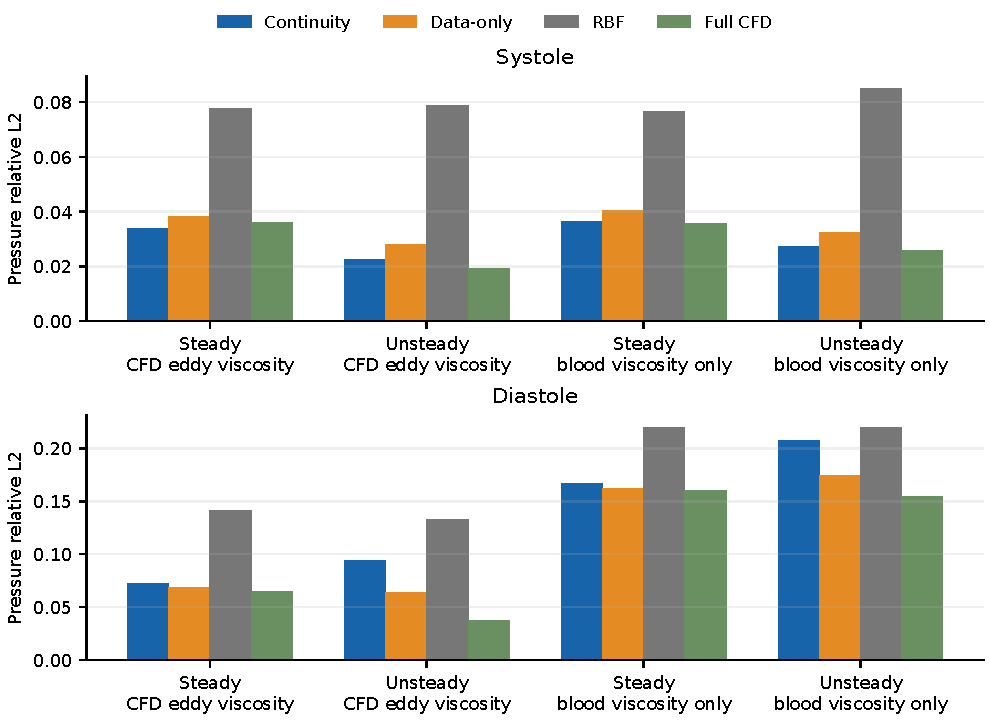
\includegraphics[width=\textwidth]{pressure_information.pdf}
\caption{Median pressure error over Cases~2--8 at 2.5~mm for the four post-processing settings. Unsteady retains the two-snapshot time derivative and steady omits it. ``\CFD eddy viscosity'' uses $\mu+\mu_t$ from the reference simulation, and ``blood viscosity only'' sets $\mu_t=0$. Full \CFD applies the same settings to the complete velocity.}
\label{fig:pressure_information}
\end{figure}

\subsection{Robustness to the choice of interpolation comparator}
\label{sec:robustness}
The prespecified \RBF used one fixed local interpolant in each snapshot. To test how much the comparison depended on that choice, we also evaluated a tuned spatial \RBF and a space-time \RBF, with their settings chosen from the withheld velocity observations. Table~\ref{tab:robustness} reports the completed comparisons for draw 0 at 2.5~mm; these values use one draw per case, so they should be compared within this table rather than directly with the three-draw means of the primary analysis.

At systole, fitting both snapshots with a space-time \RBF changed the median pressure error only slightly, from 0.079 for the prespecified \RBF to 0.074, and the \WSS error from 0.606 to 0.595. The continuity field gave errors of 0.025 and 0.356, respectively, and had lower velocity, pressure and \WSS errors than each \RBF variant in all seven cases. Tuning the spatial \RBF did not improve this phase, since its median pressure and \WSS errors were 0.127 and 0.686; therefore, choosing an interpolant by its velocity error in withheld observations did not ensure lower errors in hidden fields derived from its spatial gradients.

At diastole, both alternatives helped the interpolation. Relative to the prespecified \RBF, the tuned spatial \RBF reduced the median velocity error from 0.129 to 0.100, the pressure error from 0.136 to 0.111 and the \WSS error from 0.371 to 0.321, and the space-time \RBF reduced them to 0.096, 0.113 and 0.301. The continuity field kept lower velocity and \WSS errors than both variants in all seven cases, with a median pressure error of 0.076, but its pressure advantage held in only five of the seven diastolic cases against each variant. Over all 14 case--phase units, the continuity field had the lower pressure error in 12 against the tuned \RBF and in 12 against the space-time \RBF, with median error ratios of 0.50 and 0.54, and the lower \WSS error in all 14 against both, with median ratios of 0.54 and 0.58. It also had a lower pressure error than the better of the two variants in 12 of the 14 units. The comparison against the prespecified \RBF is therefore not an artifact of a weak interpolant, although a stronger interpolant narrows the diastolic pressure gap.

\input{tables/robustness}


\subsection{Sensitivity to near-wall observations}
\label{sec:nearwall}
Because the grid observations are snapped to mesh nodes, some lie on the near-wall prism layers (Section~\ref{sec:observations}). To measure how much the results depend on them, we repeated draw 0 at 2.5~mm for the continuity field and \RBF after removing every observation closer than $\Delta/2=1.25$~mm to the wall, which removed 28--32\% of the observations in each case (Table~\ref{tab:nearwall}). Nothing else was changed.

The \WSS errors rose sharply. For the continuity field the median rose from 0.356 to 0.806 at systole and from 0.173 to 0.521 at diastole, and for \RBF from 0.606 to 0.886 and from 0.371 to 0.681. The accuracy of the one-sided \WSS estimate therefore rests largely on velocity sampled within about a millimetre of the wall, which a 2.5~mm imaging voxel would not resolve. Pressure was much less sensitive. The continuity field's median pressure error changed from 0.025 to 0.027 at systole and from 0.076 to 0.045 at diastole, consistent with pressure being integrated only on nodes more than 1~mm from the wall. The continuity field still had lower velocity, pressure and \WSS errors than \RBF in all 14 units, so the comparison between the methods does not depend on the near-wall samples, whereas the absolute \WSS accuracy does.

\input{tables/nearwall}


\section{Discussion}
\label{sec:discussion}
\subsection{Effects of inlet diameter and asymmetry}
With the flow waveform and the maximum sac diameter held fixed, inlet diameter set the strength of the systolic disturbance and asymmetry set its location. A narrower parent vessel raised the peak Reynolds number, the jet speed entering the sac, the pressure drop, the fraction of reversed flow and the modeled eddy viscosity, and it strengthened the high-shear rings at the necks. This agrees with reports that a larger parent vessel lowers \WSS in intracranial aneurysms~\cite{fattahi2023influence}, and it extends the comparison to transitional flow in a curved, tapered thoracic segment. Because the same flow rate was prescribed for all diameters, the diameter effect here combines the change in geometry with the change in mean velocity. A study that scaled the flow rate with the vessel area would separate these two influences.

Asymmetry moved the low-shear region and the dominant vortex to the side of the larger bulge and shifted the distal high-shear region toward it, while changing the systolic pressure drop by less than 7\%. At diastole its effect became larger than that of diameter, with the asymmetric sacs carrying about two to three times the \WSS of the axisymmetric ones. A previous study of idealized abdominal and descending thoracic aneurysms also found that asymmetry mainly redistributes recirculation and \WSS~\cite{rehman2024comparative}. The present results add that the redistribution depends on the phase of the cycle, so single-instant comparisons at peak systole understate it. None of these comparisons is a population statistic, since each geometry is a single designed case, and whether low or high \WSS relates to growth or rupture cannot be settled by simulations of this kind~\cite{geers2017wall,lipp2020computational}.

\subsection{Why the neural field outperformed interpolation}
The clearest gain came from the reconstructed velocity rather than from adding momentum to the training loss. The neural fields and the prespecified \RBF received the same velocity observations and boundary values, and their pressure and \WSS were computed by the same post-processing. Yet the data field, which has no interior PDE penalty, performed close to the continuity field at 1.5 and 2.5~mm. Both neural fields also retained near-wall gradients that the prespecified \RBF tended to smooth out, and their finite-distance shear estimates recovered about 90--100\% of the \CFD 99th-percentile \WSS, compared with about half for \RBF at systole. The continuity penalty became consistently useful at the sparsest spacing, 4.0~mm.

The network fits one function across the domain and both snapshots, whereas the prespecified \RBF uses a local neighborhood at each time. This difference offers a plausible explanation for the results, but the study does not isolate the effects of spatial smoothness, joint temporal fitting and the network architecture. The space-time \RBF check narrows that interpretation, because fitting both snapshots jointly did not close the gap to the neural field at systole. At diastole, both tuning and joint temporal fitting improved all three median errors of the interpolant and reduced the continuity field's pressure advantage to five of seven cases for draw 0. These checks support the use of a neural representation in this setting without establishing that it is preferable to every interpolation scheme. Related work has used implicit neural representations for 4D flow reconstruction without a physics loss~\cite{saitta2024implicit}; here, the representation supplies velocity to the established momentum-integration route for relative pressure~\cite{krittian2012finite,bertoglio2018relative}.

The momentum \PINNs did not meet the criterion of the development test. Their poor pressure outputs, despite small momentum residuals, are consistent with a weakly determined trade-off between pressure and local acceleration. Two velocity snapshots constrain a finite difference, but they do not uniquely determine the network's time derivative between them. The diagnostic in Section~\ref{sec:pilot_results} showed that a small residual could coexist with an inaccurate pressure field. This fits the broader sensitivity of \PINNs to loss weighting and the information available to each residual~\cite{krishnapriyan2021failure,wang2021gradient}. Recovering pressure after fitting avoids relying on that pressure head, although the two-snapshot acceleration still carries reconstruction error. Longer time series, hard constraints and other loss weights might change the comparison. They were not tested here, so the negative result applies to the specified formulation and windows rather than to momentum \PINNs in general~\cite{mcgreivy2024weak}.

\subsection{Information needed for each hidden field}
Pressure and \WSS expose different weaknesses in the reconstruction of the sparse velocity. For the seven confirmation geometries, the retention of local acceleration brought the median systolic pressure error close to the complete-\CFD post-processing reference. Removing eddy viscosity did little to change that median, although the reference study of all-cases showed greater sensitivity in narrower geometries of 2.0~cm. The limited systolic sensitivity of the median should therefore not be read as evidence that eddy viscosity can always be neglected.

At diastole, omitting the \CFD eddy viscosity raised even the complete-velocity pressure error to 9--19\%. The reconstruction results with that field supplied describe a conditional calculation, because the sparse velocity observations do not themselves provide the closure. Small absolute pressure errors also matter more in this phase. None of the tested methods reliably recovered the diastolic pressure drop, even when its relative error across the field appeared modest. An estimate of eddy viscosity and a better-resolved acceleration are, therefore, separate requirements to examine before applying this calculation to measured data.

For aneurysm-zone \WSS, near-wall sampling remained the main limitation. Removing the observations within 1.25~mm of the wall more than doubled the continuity field's \WSS error at both phases while leaving the ranking against \RBF unchanged (Section~\ref{sec:nearwall}). The error depended on the distance used by the one-sided estimate, and the reconstructed fields remained above the complete-\CFD reference. Outside the aneurysm zone, the interior node closest to the wall was a median of 0.58~mm from it; even the complete \CFD velocity then gave a poor estimate of the exported shear. This is consistent with the documented sensitivity of velocity-derived \WSS to spatial resolution~\cite{petersson2012assessment,stalder2008quantitative}. A smooth velocity fit and an analytic derivative do not, by themselves, establish an accurate wall gradient.

\subsection{Limitations}
\label{Limitations}
The twelve geometries form a designed family, not a patient cohort. They share one maximum aneurysm diameter, taper ratio and inflow waveform, and they contain no branches. The seven confirmation geometries therefore test variation within that family. The rigid-wall flow solution has reported mesh, time-step and cycle checks for aneurysm \WSS, but no experimental validation. The structural calculation uses a uniform 2~mm wall, literature material parameters, fixed ends and a quasi-static coupling. Its coupling-step and mesh-update settings were not retained with the results, and no solid-mesh convergence check is available, so the stress fields are used only to describe modeled stress concentrations.

The temporal records also have limits. Each reconstruction uses two snapshots from a short window. Several instants were retained, but no complete cycle-resolved wall-traction series is available. The solver exported \TAWSS to the wall nodes, but its cycle-resolved components did not, so the oscillatory indices were not evaluated. The slice workbook does not state its averaging interval; the slice values were identified as cycle averages from the inlet flow rate.

The observed velocities are noise-free \CFD values at the mesh nodes. They do not include partial-volume averaging, noise, segmentation error, or velocity aliasing of 4D flow MRI~\cite{markl2012fourd}, and some lie within a fraction of a millimeter of the wall (Section~\ref{sec:observations}). Without observations within 1.25~mm of the wall, the \WSS errors were more than twice as large (Section~\ref{sec:nearwall}), so the absolute \WSS precision reported here should not be expected from the imaging data. Performance on measured data may therefore be worse. Pressure calculations with \CFD-supplied eddy viscosity additionally assume closure information that would have to be estimated in practice. The errors are node-weighted because the exports contain no cell volumes, which gives a greater weight to the refined near-wall mesh.

The network architecture and training settings were fixed on the development cases without a wider hyperparameter search. The tuned and space-time \RBF checks were added after the primary verdict and use one draw per case; they cannot replace the three-draw comparison. A divergence-free interpolant, the natural non-neural counterpart of the continuity field, was not tested. Every method receives observations in the target geometry. The prediction in a geometry with no observations was not tested. Finally, fitting a neural field took about 20~min on a GPU per window, so its accuracy came at a higher computational cost than interpolation.

\section{Conclusion}
\label{sec:conclusion}
Twelve idealized descending thoracic aortic geometries with a fixed maximum sac diameter of 4.0~cm were simulated with transient transitional \CFD, and their common-time fields were used both to compare the geometries and to test the recovery of hidden pressure and \WSS from sparse velocity. The inlet diameter dominated the systolic response. Reducing it from 2.6 to 2.0~cm raised the pressure drop 2.3--2.5 times, roughly doubled the fraction of reversed flow in dilation, and raised the 95th-percentile \WSS in the necks from 7--8 to 15--18~Pa, while the bulge pattern changed the drop in systolic pressure by less than 7\%. Instead, asymmetry relocated the low-shear region and the dominant vortex to the larger bulge, and at diastole it raised the median \WSS of the dilation segment 1.8--3.1 times relative to the axisymmetric sacs.

With velocity observed at about 1.3\% of the interior nodes at two instants, a continuity-constrained space-time neural field followed by momentum integration and a near-wall shear estimate recovered pressure and aneurysm-zone \WSS more accurately than the same post-processing applied to the prespecified \RBF in all 14 confirmation units after averaging three draws per unit, with median error ratios of 0.46 and 0.51. The pressure advantage was small at diastole. The benefit came mainly from the neural representation of the velocity. A continuity penalty helped in the sparsest sampling, and momentum \PINNs did not meet the development-test criterion for joint pressure and shear recovery. Systolic pressure was recovered close to the accuracy of post-processing itself, diastolic pressure required the \CFD eddy viscosity as an input to the oracle, and \WSS accuracy depended on the velocity sampled close to the wall, although the continuity field retained its advantage over \RBF without those samples. These findings identify what information each hidden field needs in this idealized, noise-free setting. Measured velocity data, estimated closures, and patient-specific anatomies are the next tests, and none of the results constitutes a clinical rupture-risk assessment.

\section*{Declarations}
\paragraph{Conflicts of interest.} The authors have no conflicts to disclose.

\ifanonymized
\paragraph{Funding and author contributions.} Removed for anonymized review.
\else
\paragraph{Funding.} Helmi Temimi thanks the Kuwait Foundation for the Advancement of Sciences (Project Code: CN22-16QE-1643).

\paragraph{Author contributions.} Conceptualization, M.A.U.R. and M.A.O.; \CFD and structural modeling, M.A.U.R.; reconstruction methodology, software and formal analysis of the reconstruction study, M.A.O.; validation, M.A.U.R., M.A.O., F.J. and H.T.; data curation, M.A.U.R. and M.A.O.; writing (original draft), M.A.U.R. and M.A.O.; writing (review and editing), all authors; funding acquisition, F.J. and H.T. All authors have read and agreed to the submitted version.
\fi


% \paragraph{Use of generative AI.} During the preparation of this work, the authors used Claude (Anthropic) and Codex (OpenAI) to help write and edit the language and grammar of the manuscript. The simulations, the study design and the interpretation of the results are the authors' own. The authors reviewed and edited all AI-assisted output and take full responsibility for the content of the publication.

\paragraph{Data availability statement.} The \CFD exports analyzed in this study are available from the corresponding author on reasonable request. \ifanonymized The reconstruction code and configuration files are available in a public repository whose link is withheld for anonymized review.\else The reconstruction code and configuration files are available at \url{https://github.com/michaelajao/IdealAorta-PINN}.\fi

\appendix
\section{Case-wise reconstruction results}
\label{app:casewise}
Tables~\ref{tab:case_pressure} and \ref{tab:case_shear} list every confirmation unit at 2.5~mm, spread over the three paired draws and the range of draw-wise error ratios to \RBF.

\input{tables/case_pressure}
\input{tables/case_shear}

\newpage
\bibliographystyle{unsrt}
\bibliography{bib/tsb,bib/references}

\end{document}
"
\newif\ifanonymized
\ifdefined\anonymized\anonymizedtrue\fi

\begin{document}

\begin{center}

{\Large \bf
% Hemodynamics of Idealized Descending Thoracic Aortic Aneurysms and Physics-Based Recovery of Pressure and Wall Shear Stress from Sparse Velocity

Effects of Inlet Diameter and Sac Asymmetry on Transitional Flow in Idealized Descending Thoracic Aortic Aneurysms, with Neural-Field Recovery of Pressure and Wall Shear Stress from Sparse Velocity
}\\[12mm]

% Continuity-Constrained Space-Time Neural Fields Improve Pressure and Wall Shear Stress Recovery from Sparse Velocity in Idealized Descending Thoracic Aortic Aneurysms

\ifanonymized\else
{\bf
M. Abaid Ur Rehman$^{a,b,*}$,
{Michael Ajao-Olarinoye$^{c}$},
Fei Jia$^{a,**}$,
Helmi Temimi$^{d}$
}\\[3mm]

{$^{a}$Department of Astronautical Science and Mechanics,
Harbin Institute of Technology, Harbin 150001, China}\\

{$^{b}$Department of Mathematics, School of Natural Sciences (SNS),
National University of Sciences and Technology (NUST),
Sector H-12, 44000, Islamabad, Pakistan}\\

{
$^{c}$Computational Science and Mathematical Modelling (CSMM),
Coventry University, Coventry, United Kingdom
}\\

{$^{d}$College of Integrative Studies,
Abdullah Al Salem University, Khaldiya, Kuwait}\\[3mm]
\fi

\end{center}

\ifanonymized\else
\noindent
$^{*}$\textbf{Corresponding author:}
M. Abaid Ur Rehman,
Email:
\href{mailto:abaidurrehman803@gmail.com}
{abaidurrehman803@gmail.com}

\vspace{1mm}

\noindent
$^{**}$\textbf{Corresponding author:}
Fei Jia,
Email:
\href{mailto:jiafei0009@163.com}
{jiafei0009@163.com}

\vspace{3mm}

\begin{center}
\textbf{Emails:}
\href{mailto:abaidurrehman803@gmail.com}
{abaidurrehman803@gmail.com},
{
\href{mailto:ajaoolarinoyemichael@gmail.com}
{ajaoolarinoyemichael@gmail.com}},
\href{mailto:jiafei0009@163.com}
{jiafei0009@163.com},
\href{mailto:helmi.temimi@aasu.edu.kw}
{helmi.temimi@aasu.edu.kw}
\end{center}
\fi

\begin{abstract}
Twelve idealized \DTAA models were constructed using three inlet diameters (\num{2.0}, \num{2.3}, and \SI{2.6}{\centi\metre}). For each inlet diameter, one axisymmetric aneurysm, two asymmetric aneurysms (anterior-dominant and posterior-dominant), and one healthy control model were considered. The maximum aneurysm diameter was fixed at \SI{4}{\centi\metre} for all aneurysmal cases, with a fixed vessel taper ratio of 0.8 from inlet to outlet. Narrowing the inlet from 2.6 to 2.0~cm increased the pressure drop from 528--561 to 1261--1346~Pa, the reverse flow fraction in dilation from 24--28\% to 50--54\%, and the 95th-percentile \WSS from 7--8 to 15--18~Pa, while the bulge pattern changed the pressure drop by at most 7\%. Instead, asymmetry relocated low \WSS to the dominant bulge and, at diastole, raised the median \WSS of the dilation segment 1.8--3.1 times above that of the axisymmetric sacs. The recovery of hidden pressure and aneurysm-zone \WSS was tested from the velocity observed at about 1.3\% of the interior nodes at two instants 5--10~ms apart. Linear and \RBF interpolation and space-time neural fields, with and without a continuity penalty, were passed through identical momentum-integration and near-wall shear calculations. Under a protocol fixed on two development geometries, the continuity-constrained field reduced pressure and \WSS errors relative to \RBF in all 14 case phase units of seven geometries not used for tuning, with median error ratios of 0.46 and 0.51, and a systolic pressure error (2.3\%) close to that from the complete \CFD velocity (1.9\%). The diastolic pressure advantage was small. The gain was mainly due to the neural representation. In two development geometries, \PINNs penalizing the residual momentum recovered pressure far less accurately than integration after fitting. Diastolic pressure required the \CFD eddy viscosity as an oracle, and \WSS accuracy required velocity sampled within about a millimeter of the wall. The results define the information each hidden field requires in idealized and noise-free conditions and are not a clinical rupture-risk assessment.
\end{abstract}
\acresetall

\noindent\textbf{Keywords.} Thoracic aortic aneurysm; computational fluid dynamics; wall shear stress; sparse flow reconstruction; physics-informed neural networks; relative pressure estimation


\section{Introduction}
\label{sec:introduction}

The cardiovascular system circulates blood throughout the body, delivering oxygen and nutrients while removing waste products~\cite{heymans1960reflexogenic}. Arteries consist of three layers~\cite{holzapfel2010modelling}: the tunica intima (innermost, endothelial cells that reduce friction), media (middle, muscular layer regulating constriction and dilation), and externa (outermost, structural support). The aorta, the largest vessel in the body, comprises the ascending aorta, the aortic arch, and the descending thoracic aorta before becoming the abdominal aorta in the diaphragm. The thoracic aorta supplies oxygenated blood to the head, neck, upper extremities, and thoracic structures~\cite{tran2018anatomy}.

Cardiovascular disease is a leading cause of mortality, affecting nearly 92 million adults in the United States and projected to affect 43.9\% of the population by 2030~\cite{Randles_CFD_2017}. Arterial disease includes atherosclerosis, stenosis, thrombus formation, and aneurysms. An aneurysm is an abnormal bulge~\cite{Les_et_al_2010}, classified as saccular (one-sided) or fusiform (circumferential)~\cite{sakalihasan2018abdominal}. Elective repair is often determined by maximum diameter, with various anatomical factors proposed as predictors of severity~\cite{cronenwett1990variables, lipp2020computational}. However, these standards lack precision: aneurysms of the same maximum diameter can vary in shape, wall thickness, and mechanical properties, affecting growth and risk of rupture. A surgery based on a 5~cm criterion may therefore be unjustifiable or delayed inappropriately, since rupture can occur below this threshold~\cite{darling1977autopsy, belkacemi2022flow}. Since rupture occurs when mechanical stress exceeds tissue tensile strength, risk assessment based on \WSS and hemodynamics provides more accurate prediction~\cite{bilgi2020effects, vorp1998mechanical}. Kitagawa et al.~\cite{kitagawa2013role} further suggest that aneurysm volume is more reliable than maximum diameter because it captures the entire 3D shape and detects subtle growth more consistently.

\CFDcap plays an important role in the study of vascular disease progression, particularly blood flow behavior in abnormal arteries~\cite{lee2011computational}. It uses numerical methods to solve the Navier--Stokes equations for flow fields, velocity, and stresses~\cite{navier1823memoire, stokes2007theories}, aiding early diagnosis and risk assessment~\cite{morris2016computational}. Commonly used parameters include \WSS, \WSSG, and \OSI. Both high and low \WSS are associated with aneurysm disease: high \WSS contributes to initiation by weakening the intima, while low \WSS promotes growth and rupture~\cite{geers2017wall}. Moon et al.~\cite{moon2025hemodynamic} studied four ruptured fusiform infrarenal aneurysms and found rupture in regions of low \TAWSS, high \OSI, \RRT, and \ECAP. Kumar et al.~\cite{SK1} reported that saccular aneurysms exhibit complex streamline patterns and low-\WSS regions.

Arterial tortuosity, the bending and twisting of vessels, alters local flow patterns and causes disturbed hemodynamics~\cite{9a}. Inflow conditions, and thus velocity and \WSS distributions, are determined by parent vessel diameter, which feeds the aneurysm. These geometric factors jointly regulate intra-aneurysmal flow, affecting growth, thrombosis, and rupture. Buradi et al.~\cite{10a} analyzed idealized tortuous geometries, varying curvature radius, bending angle, and inter-bend distance, and found that regions with high \RRT, significant \TAWSS gradient, and lower \OSI are more susceptible to plaque development and rupture. Nagargoje et al.~\cite{11a} modeled C-, U-, S-shaped, and helical \ICA bends, concluding that parent artery morphology significantly affects local hemodynamics. Tortuosity effects have also been studied in abdominal~\cite{12a}, descending thoracic~\cite{13a}, and cerebral aneurysms~\cite{14a}. Fattahi et al.~\cite{fattahi2023influence, fattahi2023usage} found that increasing parent-vessel diameter decreases \WSS and \OSI in \ICA sacs. Nagargoje et al.~\cite{nagargoje2022influence} showed that increasing \AR and \SR raises near-neck \WSS, \OSI, and \RRT in patient-specific models.

Laminar flow is typical in a healthy aorta, but aneurysms introduce irregular geometries and pulsatile flow that disturb the streamlines. Transitional or turbulent flow occurs in clinical conditions such as aneurysms and other vascular diseases, and the resulting instabilities and vortex structures require turbulence models for accurate hemodynamic analysis. Brambila-Solórzano et al.~\cite{brambila2023influence} discussed how turbulent modeling affects \WSS and \TAWSS prediction in aneurysms, which is crucial for identifying high-risk rupture regions. Turbulence models such as $k-\epsilon$ or \DNS resolve chaotic flow structures and better estimate pressure drop, flow separation, and vortex formation. Such modeling is vital for capturing complex unstable patterns overlooked by laminar assumptions, particularly in regions with disturbed flow. These disturbances often lead to transitional or turbulent flow even at moderate Reynolds numbers~\cite{evju2015assumption}, particularly within aneurysmal regions. Luciano et al.~\cite{luciano2024turbulent} investigated turbulence in cerebral aneurysms despite low sac Reynolds numbers, noting that neglecting turbulent effects can introduce errors. Rawat et al.~\cite{rawat2019numerical} similarly emphasized that arterial flow can be transitional, with vortices forming after systole. Accurate turbulent flow modeling is therefore essential for capturing hemodynamic parameters such as \WSS and \OSI.

Several studies have investigated aneurysm hemodynamics using patient-based and idealized geometries. Lauric et al.~\cite{lauric2019proximal} examined 33 middle cerebral artery aneurysm patients and 44 controls, finding aneurysmal arteries have a tapered parent vessel (mean ratio 0.88) versus near-unity in healthy vessels; tapering elevates \WSS and \WSSG, promoting aneurysm formation. Jin et al.~\cite{jin2023cfd} reported that reducing coil porosity from 0.89 to 0.79 decreases \OSI by up to 55\% in an \ICA aneurysm. Tian et al.~\cite{tian2023influence} used 18 idealized and 7 patient-specific bifurcation aneurysms to show that the aneurysm--parent vessel angle dominates \LDL deposition, with larger angles promoting deposition by reducing inflow and enhancing stagnation. Rehman et al.~\cite{ur2025fluid} studied Marfan syndrome aneurysms using \FSI with \CFD and \PINNs on six patient-specific models, observing that \WSS disturbances vary with shape and that the anterior wall experiences higher stresses. Zhou et al.~\cite{zhou2026morphological} developed an AutoML model on 158 intracranial aneurysms, identifying bifurcation angle as the most critical risk factor. These patient-based studies, however, are confounded by multiple simultaneously varying anatomical features, making it difficult to isolate single-parameter effects. Idealized geometries offer systematic parameter variation.

Previous idealized studies have largely overlooked physiological tapering (i.e., the progressive reduction in vessel diameter from inlet to outlet), the isolated influence of parent vessel diameter, and the relationship between hemodynamic and morphometric characteristics of the aorta for both axisymmetric (fusiform) and asymmetric (saccular) geometries of \DTAA (Table~\ref{tab:lit_review}). To address these gaps, the present study introduces a set of twelve idealized geometries of the descending thoracic aorta, including nine with aneurysms and three healthy ones without aneurysms. The entire vessel, from inlet to outlet, is modeled with a linear taper characterized by a fixed taper ratio of 0.8 (i.e., outlet diameter $= 0.8 \times$ inlet diameter), consistent with physiological observations. Three different diameters of inlets (2.0~cm, 2.3~cm and 2.6~cm) are used to study the effect of parent vessel size, and a localized aneurysm is simulated with a fixed maximum diameter of 4~cm in the descending thoracic segment. For each inlet diameter, three aneurysm morphologies are examined, namely axisymmetric (fusiform), anterior-dominant asymmetric (saccular), and posterior-dominant asymmetric (saccular), reflecting clinically observed variations. Unlike the ascending aorta, the descending thoracic aorta is characterized by an upstream curvature, significantly affecting the flow dynamics upstream of aneurysm formation. Thus, in this study, the investigation of parent vessel diameter and physiological tapering, aneurysm asymmetry, and flow dynamics in \DTAA is considered.

Resolving each of these geometries with \CFD is computationally demanding, which limits how densely the diameter--asymmetry space can be sampled and how readily the analysis extends to a new vessel size. The same fields also raise a second, methodological question, because the quantity that is measured clinically is velocity, not pressure or \WSS. Time-resolved three-dimensional phase-contrast MRI (4D flow MRI) samples the lumen on voxels of roughly one to three millimeters~\cite{markl2012fourd}, whereas relative pressure and \WSS have to be derived from those samples. Relative pressure can be computed from measured velocity by pressure-Poisson, work--energy and related formulations of the momentum balance~\cite{krittian2012finite, bertoglio2018relative}, and \WSS estimated from phase-contrast velocity depends strongly on spatial resolution and wall segmentation and is usually underestimated~\cite{stalder2008quantitative, petersson2012assessment, potters2015volumetric}. \PINNs and related neural fields offer another route, fitting a continuous representation to sparse velocity while penalizing violations of the governing equations~\cite{raissi2019pinn, raissi2020hfm}. They have been used to infer arterial pressure from 4D flow data~\cite{kissas2020machine}, to super-resolve and denoise 4D flow fields~\cite{fathi2020super, saitta2024implicit}, to recover near-wall flow and \WSS from sparse velocity~\cite{arzani2021nearwall} and to reconstruct aneurysm flow~\cite{cruzgonzalez2025aaa}. \PINN training can fail for reasons unrelated to the available information~\cite{krishnapriyan2021failure, wang2021gradient}, and a survey of machine learning for fluid-related partial differential equations found that most reported advantages were measured against weak baselines~\cite{mcgreivy2024weak}.

Two points are rarely separated in this literature, and both matter in pulsatile transitional flow. The first is how much of any improvement over conventional interpolation comes from the neural representation itself and how much from the physics terms added to its loss. The second is what information beyond sparse velocity the hidden fields actually require, because in unsteady Reynolds-averaged flow the pressure gradient also depends on local acceleration and on the eddy viscosity, neither of which is measured directly. A fair test needs matched observations for every method, one shared route from velocity to pressure and \WSS, and an explicit account of every additional input. Table~\ref{tab:lit_review} compares the present study with earlier idealized aneurysm studies on these points and on the modeling choices discussed above.


\begin{table}[htbp]
\centering
\footnotesize
\caption{Comparison of existing idealized aneurysm studies and the present work, emphasizing differences in geometry, flow modeling, boundary conditions, hemodynamic--morphometric analysis, and sparse-velocity reconstruction.}
\setlength{\tabcolsep}{3pt}
\begin{tabular}{|>{\raggedright\arraybackslash}p{4.0cm}|*{6}{>{\centering\arraybackslash}p{1.78cm}|}}
\hline
\textbf{Feature} & \parbox{1.78cm}{\textbf{Jin et al.~\cite{jin2021arterial}}} & \parbox{1.78cm}{\textbf{Guerrero-Hurtado et al.~\cite{guerrero2023efficient}}} & \parbox{1.78cm}{\textbf{Rehman et al.~\cite{rehman2024comparative}}} & \parbox{1.78cm}{\textbf{Rehman et al.~\cite{rehman2025application}}} & \parbox{1.78cm}{\textbf{Moroni \& Espa~\cite{moroni2025insight}}} & \parbox{1.78cm}{\textbf{Present Study}} \\
\hline
Year & 2021 & 2023 & 2024 & 2025 & 2025 & - \\
\hline
Geometry Type & Idealized & Idealized & Idealized & Idealized & Idealized & Idealized \\
\hline
\DTAA & No & No & Yes & No & No & Yes \\
\hline
{Arterial Tapering} & No & No & No & No & No & Yes \\
\hline
Parent vessel effect & No & No & No & No & No & Yes \\
\hline
\parbox{3.7cm}{Morphology: Axisymmetric or Asymmetric} & Not varied & Not varied & Both & Both & Both & Both \\
\hline
\parbox{3.7cm}{SST $k-\omega$ Transition Turbulence Model} & No & No & No & No & No & Yes \\
\hline
Transient Flow Inlet & Yes & Yes & No & No & No & Yes \\
\hline
\parbox{3cm}{Transient Pressure Outlet} & Yes & No & No & No & No & Yes \\
\hline
Plane-wise flow--morphometry analysis & Partial & No & No & Partial & Partial & Yes \\
\hline
\PINNcap & No & No & Yes & No & No & Tested on two cases \\
\hline
Hidden pressure and \WSS from sparse velocity against matched baselines & No & No & No & No & No & Yes \\
\hline
\end{tabular}%
\label{tab:lit_review}
\end{table}



This study addresses both questions on a family of twelve idealized descending thoracic aortic geometries, namely nine aneurysmal models formed by three inlet diameters and three bulge patterns at a fixed 4.0~cm maximum sac diameter, and three nonaneurysmal controls. The contributions are as follows.
\begin{enumerate}
\item We report how inlet diameter and sac asymmetry change pressure drop, reversed flow, eddy viscosity and aneurysm-zone \WSS in transient transitional \CFD, evaluated at common systolic and diastolic instants for all twelve geometries.
\item We define a sparse-reconstruction task on the same fields, in which velocity is observed at about 1.3\% of the interior nodes at two instants 5--10~ms apart and hidden pressure and aneurysm-zone \WSS must be recovered in the known geometry. Linear interpolation, \RBF interpolation and space-time neural fields with and without a continuity penalty all pass through the same momentum-integration and near-wall shear calculations, so their differences are attributable to the reconstructed velocity alone.
\item Using a protocol fixed on two development geometries before evaluation on seven others, we separate the contributions of the neural representation, the continuity constraint, the local time derivative and the eddy-viscosity closure. On two development geometries, we also report that the pressure output of a \PINN with the momentum residual in its loss was far less accurate than momentum integration applied after fitting.
\end{enumerate}
The two parts belong together because the parametric family supplies reference fields whose jet strength, recirculation and modeled eddy viscosity vary systematically with geometry, so the reconstruction test can show how recovery depends on these flow features rather than on a single case. The reconstruction concerns a known geometry with noise-free velocity sampled from \CFD. It does not test prediction for an unseen anatomy, and it does not establish clinical rupture risk.


\section{\label{Material and Methods}Materials and methods}
\subsection{\label{Geometric Description}Geometric description}
Twelve idealized descending-aortic geometries were examined, namely nine aneurysmal models and three nonaneurysmal (healthy) controls. The aneurysmal group used three inlet diameters, 2.0, 2.3 and 2.6~cm. An axisymmetric and two asymmetric aneurysm shapes were studied for each inlet diameter. The level of asymmetry was calculated as the ratio $\beta = r/R$, where $r$ and $R$ denote the characteristic radii of the aneurysmal segment in the posterior and anterior directions, respectively. An axisymmetric bulge gives $\beta = 1$; {a} posterior-dominant bulge gives $\beta > 1$ and {an} anterior-dominant bulge $\beta < 1$, the two representing opposite directional dilations. The detailed geometric parameters are given in Table~\ref{tab:geometries}. To compare with the healthy models, the other three models that have the same inlet diameters (2.0~cm, 2.3~cm and 2.6~cm) were also built. In these control cases no aneurysmal dilation was added and, as in the aneurysmal models, the vessels were tapered smoothly along their lengths, with a physiologically consistent reduction in diameter so that the outlet diameter is 80\% of the inlet diameter. The twelve cases therefore form three groups by inlet diameter, each containing three aneurysmal cases and their matching control. Group~1 (2.0~cm) comprises Cases~1--3 and control Case~10, Group~2 (2.3~cm) comprises Cases~4--6 and control Case~11, and Group~3 (2.6~cm) comprises Cases~7--9 and control Case~12. Case numbers are used throughout, and each control is compared with the aneurysmal cases of its own group.

The eight cross-sectional planes (D1--D8) shown in Figure~\ref{fig:diagram} were used to investigate the spatial variations of the hemodynamic parameters along the arterial axis. All the aneurysmal models had a single dilation centered at the mid-region (D5) and the maximum aneurysm diameter was set at 4.0~cm for all the diseased aneurysm cases. The (D1--D4) and (D6--D8) represent the upstream and downstream portions of the aneurysms. The average diameters of the planes are listed in Table~\ref{tab:diameter}. Two section planes are used throughout, the medial plane ($xy$-plane) and the transverse plane ($xz$-plane) through the axis of the descending segment. Every model is mirror-symmetric about the medial plane, and the anterior--posterior asymmetry of the bulge lies within that plane.



\begin{table}[htbp]
\centering
\caption{\AANcap models considered in the present study. Here $r$ and $R$ are the {posterior and anterior} characteristic radii of the sac and $\beta = r/R$ is the directional asymmetry ratio. Each group collects the three aneurysmal cases of one inlet diameter and their control.}
\label{tab:geometries}
\setlength{\tabcolsep}{4pt}
\begin{tabular}{ll ccc ccc}
\toprule
& & \multicolumn{3}{c}{Sac geometry}
  & \multicolumn{3}{c}{Case ID by inlet diameter \(D_{\mathrm{in}}\)} \\
\cmidrule(lr){3-5} \cmidrule(lr){6-8}
& & & & & Group~1 & Group~2 & Group~3 \\
Type & Configuration & \(r\) (cm) & \(R\) (cm) & \(\beta = r/R\)
     & 2.0 cm & 2.3 cm & 2.6 cm \\
\midrule
Axisymmetric & --         & 2.0 & 2.0 & 1.00 & 1  & 4  & 7  \\
Asymmetric   & Ant.-dom.  & 1.3 & 2.7 & 0.48 & 2  & 5  & 8  \\
             & Post.-dom. & 2.7 & 1.3 & 2.08 & 3  & 6  & 9  \\
Control      & --         & --  & --  & --   & 10 & 11 & 12 \\
\bottomrule
\end{tabular}
\end{table}
\begin{table}[htbp]
\centering
\caption{Plane diameter (cm), mean $\pm$ standard deviation across the nine aneurysmal and three control geometries.}
\begin{tabular}{lcc}
\toprule
Plane & Aneurysmal ($n=9$) & Control ($n=3$) \\
\midrule
D1 & 2.28 $\pm$ 0.26 & 2.28 $\pm$ 0.30 \\
D2 & 2.22 $\pm$ 0.25 & 2.22 $\pm$ 0.29 \\
D3 & 2.15 $\pm$ 0.24 & 2.15 $\pm$ 0.28 \\
D4 & 2.97 $\pm$ 0.09 & 2.11 $\pm$ 0.28 \\
D5 & 4.00 $\pm$ 0.00 & 2.08 $\pm$ 0.27 \\
D6 & 2.92 $\pm$ 0.09 & 2.05 $\pm$ 0.27 \\
D7 & 2.02 $\pm$ 0.23 & 2.02 $\pm$ 0.26 \\
D8 & 1.95 $\pm$ 0.22 & 1.95 $\pm$ 0.25 \\
\bottomrule
\end{tabular}
\label{tab:diameter}
\end{table}


 \begin{figure}[ht!]
         \centering
         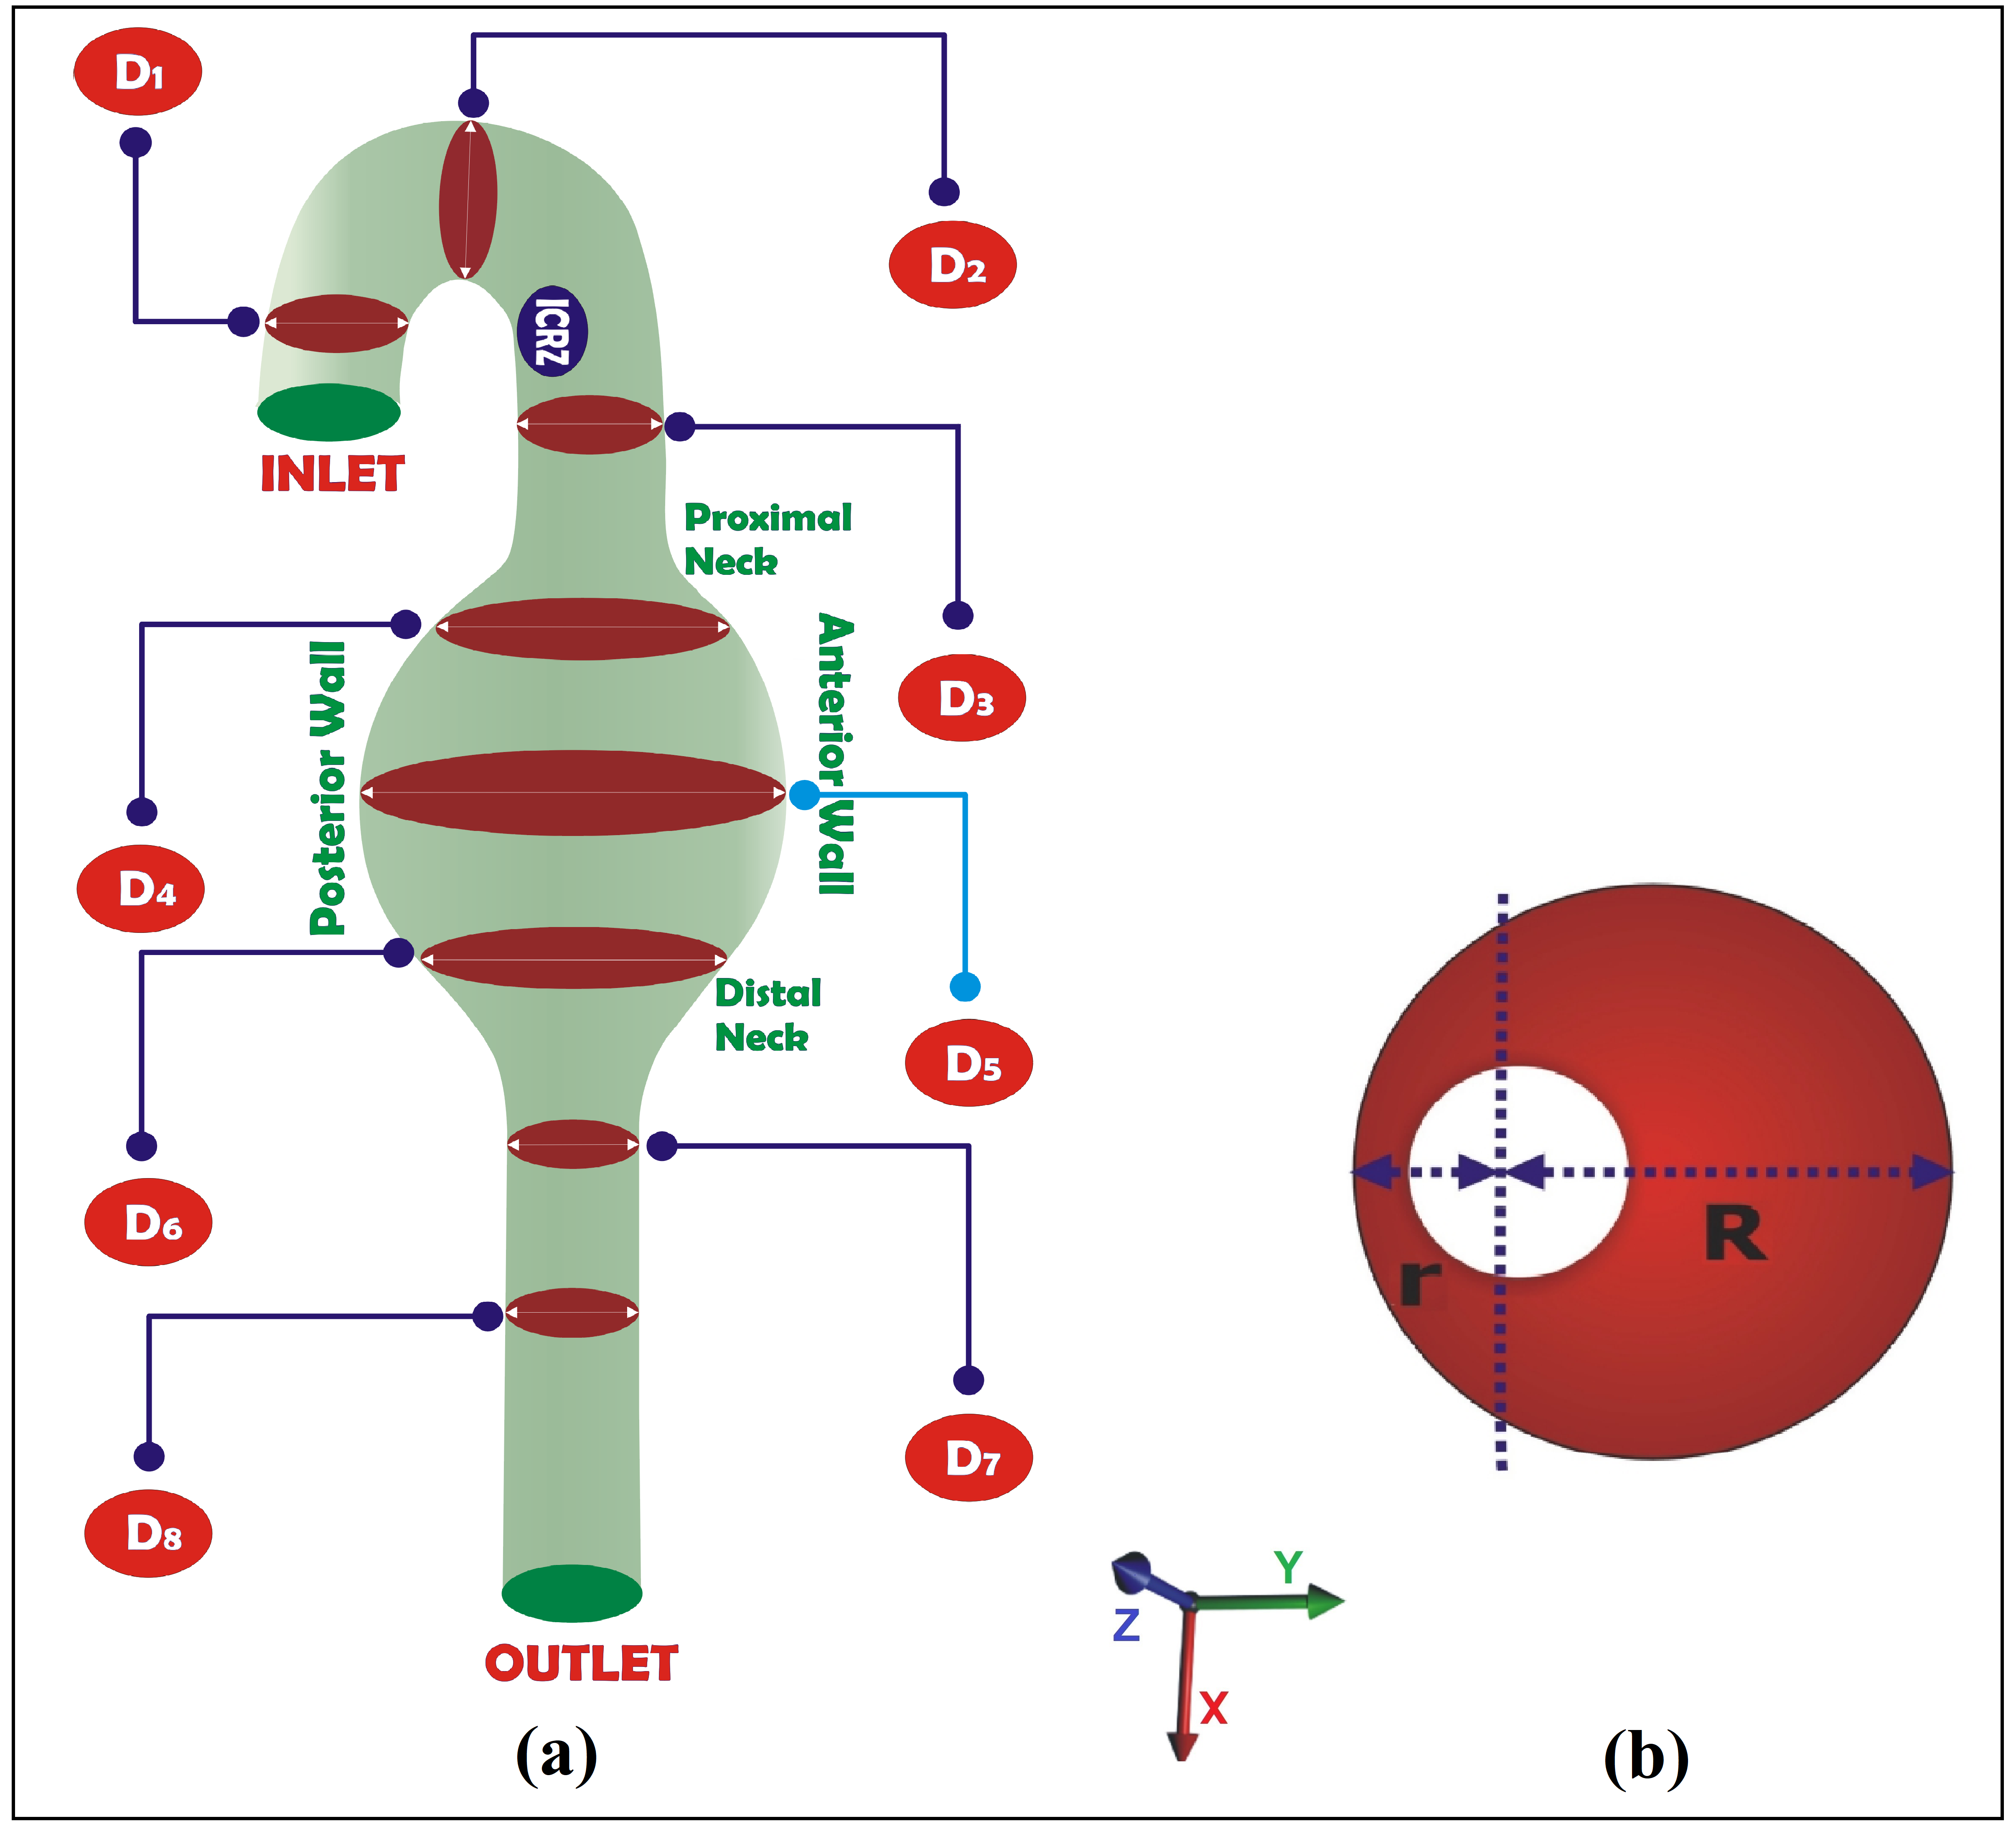
\includegraphics[width=1\textwidth, height=0.7\textheight]{Geometry.png}
         \caption{Visual depictions of (a) the three-dimensional geometry of the aneurysm and (b) the cross-sectional area of the aneurysm sac.}
         \label{fig:diagram}
     \end{figure}

     
\hspace*{\parindent} 

\subsection{\label{sec:governing_equations}Blood flow modeling and boundary conditions} 
\subsubsection{Governing equations and turbulence modeling}

The incompressible Navier--Stokes equations, which govern blood flow, are given by \cite{navier1823memoire, stokes2007theories}:
\begin{align}
    \nabla \cdot \mathbf{v} &= 0, \label{eq:cont}\\
    \rho \left( \frac{\partial \mathbf{v}}{\partial t} + (\mathbf{v} \cdot \nabla) \mathbf{v} \right) &= -\nabla p + \mu \nabla^2 \mathbf{v}, \label{eq:ns}
\end{align}
where \(\rho\) is the fluid density, \(\mathbf{v}\) the velocity vector, \(p\) the pressure, and \(\mu\) the dynamic viscosity.

For the unsteady Reynolds-averaged calculation, the instantaneous velocity will be decomposed as $\mathbf v=\mathbf V+\mathbf v'$ with $\overline{\mathbf v'}=0$, where $\mathbf V$ is the mean velocity. The Reynolds stress is closed by the Boussinesq eddy-viscosity approximation,
\begin{equation}
-\rho\overline{v_i'v_j'}=\mu_t\left(\partial_j V_i+\partial_i V_j\right)-\frac{2}{3}\rho k\delta_{ij},
\label{eq:boussinesq}
\end{equation}
where $k=\tfrac12\overline{v_i'v_i'}$ is \TKE per unit mass (m$^2$~s$^{-2}$), $\mu_t$ is dynamic eddy viscosity, and $\delta_{ij}$ is the Kronecker delta. With Eq.~\eqref{eq:boussinesq}, the Reynolds-averaged momentum equation solved for the mean velocity and pressure $P$ is
\begin{equation}
\rho\left(\frac{\partial\mathbf V}{\partial t}+(\mathbf V\cdot\nabla)\mathbf V\right)=-\nabla P+\nabla\cdot\left[(\mu+\mu_t)\left(\nabla\mathbf V+\nabla\mathbf V^{T}\right)\right]-\frac{2}{3}\nabla(\rho k),
\label{eq:urans}
\end{equation}
with $\nabla\cdot\mathbf V=0$.

\subsubsection{\texorpdfstring{\SSTcap \(k\)--\(\omega\) transition model}{SST k-omega transition model}}

The \SST \(k\)--\(\omega\) transition model was employed to account for the possible transition from laminar to turbulent flow and to capture the complex flow features associated with curvature, flow separation, and recirculation in the descending thoracic aorta. The model combines the near-wall formulation of the \(k\)--\(\omega\) model with the free-stream behavior of the \(k\)--\(\epsilon\) formulation through appropriate blending functions.

The turbulent eddy viscosity is calculated as
\begin{equation}
    \mu_t =
    \frac{a_1 \rho k}
    {\max(a_1\omega,\;SF_2)},
    \label{eq:mutt}
\end{equation}
where \(k\) is the \TKE, \(\omega\) is the specific dissipation rate, \(S\) is the magnitude of the strain-rate tensor, and \(F_2\) is the second blending function.

The transport equations for \TKE and specific dissipation rate are given by
\begin{equation}
\frac{\partial(\rho k)}{\partial t}
+\nabla\cdot(\rho k\mathbf{V})
=
\nabla\cdot
\left[
\left(\mu+\frac{\mu_t}{\sigma_k}\right)\nabla k
\right]
+P_k-D_k,
\label{eq:keqn}
\end{equation}

\begin{equation}
\frac{\partial(\rho\omega)}{\partial t}
+\nabla\cdot(\rho\omega\mathbf{V})
=
\nabla\cdot
\left[
\left(\mu+\frac{\mu_t}{\sigma_\omega}\right)\nabla\omega
\right]
+P_\omega-D_\omega
+
2(1-F_1)\rho\sigma_{\omega2}
\frac{1}{\omega}
\frac{\partial k}{\partial x_j}
\frac{\partial\omega}{\partial x_j}.
\label{eq:omegaeqn}
\end{equation}

Unlike the standard \SST \(k\)--\(\omega\) model, the transition formulation additionally solves two transport equations: one for the intermittency \(\gamma\), which varies from zero in laminar regions to unity in fully turbulent regions, and another for the transition momentum-thickness Reynolds number \(\widetilde{Re}_\theta\). These variables enable the model to predict the onset and development of boundary-layer transition based on the local flow conditions.

The blending functions \(F_1\) and \(F_2\) regulate the transition between the \(k\)--\(\omega\) and \(k\)--\(\epsilon\) formulations. \(F_1\) provides the appropriate near-wall blending, whereas \(F_2\) limits the eddy viscosity in regions where strain-rate effects become important. The distance to the nearest wall is denoted by \(y\). Thus, the \SST \(k\)--\(\omega\) transition model combines the strong near-wall behavior of the \(k\)--\(\omega\) formulation with the reduced free-stream sensitivity of the \(k\)--\(\epsilon\) formulation in the outer region of the boundary layer, while the additional intermittency and transition-Reynolds-number equations allow laminar--turbulent transition to be represented.




\subsubsection{Boundary conditions}
The pulsatile flow rate at the inlet is used in order to replicate the pulsatile nature of the blood flow in the human body. The inlet profile is expressed as:

\begin{equation}
Q(t)=
\begin{cases}
Q_0\,\sin\!\left(\dfrac{\pi\,(t-nT)}{0.35}\right)+0.05\,Q_0,
& nT \le t \le nT+0.35, \\[6pt]
0.05\,Q_0,
& nT+0.35 < t \le (n+1)T.
\end{cases}
\end{equation}


Similarly, the pulsatile outlet pressure is used at the outlet and is

\begin{equation}
P(t) =
\begin{cases} 
P_\mathrm{min} + \left(P_\mathrm{max} - P_\mathrm{min}\right) \, \sin\left(\dfrac{\pi \, (t - \, n \, T)}{0.35}\right), & nT \le t \le nT+0.35, \\
P_\mathrm{min}, & nT+0.35 < t \le (n+1)T.
\end{cases}
\end{equation}

Here $P_{\mathrm{min}}=80$~mmHg, $P_{\mathrm{max}}=120$~mmHg, $n=0,1,2,3$ indexes cardiac cycles, $T=0.8$~s, and $Q_0=2.39\times10^{-4}$~m$^3$~s$^{-1}$ is the sinusoidal amplitude. Because of the $0.05Q_0$ offset, the actual peak of the prescribed inlet flow rate is $1.05Q_0$.

{The inlet flow-rate and outlet pressure profiles that these two equations define are shown in Figure~\ref{fig:profiles}.}

\begin{figure}[!htb]
\centering
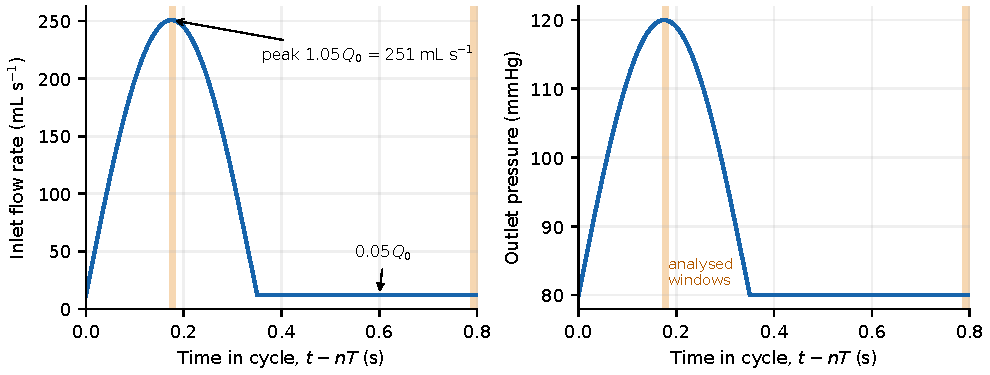
\includegraphics[width=\textwidth]{bc_profiles.pdf}
\caption{Prescribed inlet flow rate (left) and outlet pressure (right) over one cardiac cycle.}
\label{fig:profiles}
\end{figure}

At the wall no slip condition is applied.



\subsubsection{\label{sec:Hemodynamics Parameters}Hemodynamic parameters}

\hspace*{\parindent} \WSScap  denotes the tangential force per unit area applied by blood flow against the vessel wall. The \WSS for vessels \cite{potters2015volumetric} can be calculated using the formula:

\begin{align}
    \tau_w = \mu \left. \frac{\partial {u_t}}{\partial n} \right|_{n=0},
\end{align}

where \(\mu\) is the blood viscosity, \(\frac{\partial {u_t}}{\partial n}\) is the {tangential velocity gradient} in the direction \(n\) normal to the wall, and {\(u_t\) is the local tangential velocity component at the wall}.

To characterize the temporal and directional features of \WSS over a cardiac cycle, two additional metrics were computed on the aneurysm wall \cite{morbiducci2010outflow, turk2021characterization}:
\begin{equation}
\text{\TAWSScap} = \frac{1}{T} \int_{0}^{T} \left| \mathbf{WSS}(\mathbf{s},t) \right| \, dt,
\end{equation}
where $T$ is the duration of one cardiac cycle and $\mathbf{s}$ denotes a point on the vessel wall. \TAWSS  represents the magnitude of the \WSS vector averaged over time.

\TKEcap was quantified to assess the level of turbulence in the aneurysm sac, in addition to \WSS and \TAWSS. Here, \TKE represent the fluctuating components of the velocity field in the three coordinate directions. It provides an indicator of turbulence intensity and has been associated with increased flow instability and potential damage to the aneurysmal wall.

Additionally, velocity magnitudes were determined at eight predetermined cross-section planes (D1--D8) across the arterial axis and examined the spatial development of flow and its association with local vessel geometry. This was an analysis based on planes which allowed the direct correlation between morphometric parameters (diameter) and hemodynamic quantities (velocity, \TKE).


\MPScap was calculated on the inner surface of the aneurysmal wall to assess the structural response of the artery wall under pressure loading. \MPS represents the highest tensile principal stress at a given point and is commonly used in biomechanical studies as an indicator of rupture risk, because wall failure is expected when the local tensile stress exceeds the local tissue strength. The stress tensor was computed throughout the structural domain, and the spatial distribution of \MPS was analyzed to identify regions of elevated wall stress that may be more susceptible to mechanical failure.

\subsubsection{\label{CFD Simulation}\texorpdfstring{\CFDcap}{CFD} simulation}ANSYS Fluent, a commercial finite-volume solver with a pressure-based formulation, was used to solve the governing equations for mass and momentum conservation. Blood was modeled as an incompressible Newtonian fluid with density \(\rho = 1050\,\mathrm{kg\,m^{-3}}\) and dynamic viscosity \(\mu = 3.5 \times 10^{-3}\,\mathrm{Pa\,s}\).


The spatial convergence of the steady flow results was checked by performing a mesh refinement study. Prescribed flow rate was \(2.39 \times 10^{-4} \, \mathrm{m^3/s}\) and the \SST \(k\)-\(\omega\) turbulence model was used. Four different meshes (2.9~mm to 0.8~mm) were used in the testing as shown in (Table~\ref{tab:mesh_study}). The relative change, Richardson-extrapolated value and \GCI were computed between each mesh and the immediately finer mesh. The assumed second order convergence rate, $p=2$ was used in conjunction with Roache's conservative safety factor, $F_s=3.0$ for the evaluation of the \GCI. The two first refinements had relatively high \GCI values, which means that the coarser meshes were not in the range of mesh independent solution. For comparison, refinement from 1.3~mm to 0.8~mm changed the maximum aneurysmal \WSS by only 0.89\%, was Richardson extrapolated to 66.83~Pa, and had a fine-grid \GCI value of 1.63\%. Therefore, the 0.8~mm mesh was selected for the final simulations.

\begin{table}[ht!]
\centering
\setlength{\tabcolsep}{3.5pt}
\caption{Reported steady-flow fluid-mesh refinement for maximum aneurysmal \WSS. The extrapolation assumes second-order convergence.}
\label{tab:mesh_study}
\setlength{\tabcolsep}{7pt}
\begin{tabular}{cccccc}
\toprule
Element & Number of & Maximum & Relative & Richardson- & GCI$_{\rm fine}$ \\
size & elements & aneurysm & change & extrapolated & (\%) \\
(mm) & & \WSS (Pa) & (\%) & \WSS (Pa) & \\
\midrule
2.9 & 62\,261    & 47.8 & --    & --    & -- \\
1.9 & 196\,142   & 55.4 & 13.72 & 61.12 & 30.95 \\
1.3 & 578\,040   & 67.8 & 18.29 & 78.71 & 48.29 \\
0.8 & 1\,475\,430 & 67.2 & 0.89  & 66.83 & 1.63 \\
\bottomrule
\end{tabular}
\end{table}


The temporal convergence was evaluated for three different time step sizes: 0.01~s, 0.001~s, and 0.0005~s. The difference between the two smaller time steps was small, less than 2\%, and there was very good agreement in the \WSS waveforms. The time step was chosen as 0.001~s, which was found to be adequate in terms of both the level of temporal resolution and computational efficiency.

To eliminate initial transient effects and ensure a periodic steady state, the simulations were run for four consecutive cardiac cycles (\(n = 0,1,2,3\)). The percentage difference in \WSS between the third and fourth cycles was negligible (mean \(< 0.4\%\)), confirming that a periodic steady state had been reached. Accordingly, results from the third cardiac cycle were used for all subsequent analyses.



\subsubsection{Fluid--structure interaction model}

The arterial wall was modeled using ANSYS mechanical and considered as a nearly incompressible, isotropic hyperelastic material using the second-order Yeoh strain energy potential. The strain energy density function is
\begin{equation}
W = C_{10}(\bar{I}_1 - 3) + C_{20}(\bar{I}_1 - 3)^2,
\label{eq:yeoh}
\end{equation}
where \(W\) is the strain energy density, \(\bar{I}_1\) is the first deviatoric strain invariant, and \(C_{10}\) and \(C_{20}\) are material constants. The material constants were set to \(C_{10} = 98.8~\text{kPa}\) and \(C_{20} = 779.1~\text{kPa}\) \cite{zhu2025combined}. The incompressibility parameter \(D_1\) was specified as \(2.04 \times 10^{-4}~\text{kPa}^{-1}\), corresponding to a Poisson's ratio of \(\nu = 0.49\). A uniform wall thickness of 2.0~mm was assumed for all models, consistent with previous idealized \FSI studies of thoracic \AANs, and the arterial wall density was set to 1120~kg/m\(^3\).

To represent the physiological fixation of the artery, fixed boundary conditions were applied at both the inlet and outlet. The \FSI  interface was defined on the inner surface of the arterial wall to enable bidirectional coupling between the fluid and structural domains. The computational workflow is presented in Figure~\ref{fig:Flowchart}.



\begin{figure}[!ht]
  \centering
  \definecolor{cIn}{HTML}{1F6FB2}
  \definecolor{cNet}{HTML}{0E8C84}
  \definecolor{cData}{HTML}{C0392B}
  \definecolor{cPhys}{HTML}{B07A12}
  \definecolor{cPost}{HTML}{2E7D32}
  \definecolor{cOpt}{HTML}{555555}
  \resizebox{\textwidth}{!}{%
  \begin{tikzpicture}[
      font=\small,
      >={Stealth[length=2.2mm]},
      box/.style={rounded corners=2pt, draw=#1!70, line width=0.6pt, fill=#1!7,
                  align=center, inner sep=4pt, text=black, minimum width=52mm, minimum height=9mm},
      dec/.style={diamond, aspect=2.2, draw=cOpt!70, fill=cOpt!7, line width=0.6pt, inner sep=1.5pt, font=\small},
      arr/.style={->, draw=black!65, line width=0.7pt},
      lab/.style={font=\footnotesize, text=black!70},
      ilab/.style={font=\footnotesize\itshape, text=black!60},
    ]

    % ---------------------------------------------------------
    % Top: geometry
    % ---------------------------------------------------------
    \node[box=cOpt, minimum width=60mm] (geo) {\textbf{Geometry}: Twelve idealized models};

    % ---------------------------------------------------------
    % Left column: fluid
    % ---------------------------------------------------------
    \node[box=cIn, below left=8mm and -14mm of geo] (fl) {\textbf{Fluid (blood)}: ANSYS Fluent};
    \node[box=cIn, below=4mm of fl] (fmesh) {Mesh generation};
    \node[box=cIn, below=4mm of fmesh, align=center] (fset) {%
        Fluid properties and boundary conditions.\\
        Discretization method and convergence setup.};
    \node[dec, below=5mm of fset] (conv) {converged?};
    \node[box=cIn, below=6mm of conv] (fres) {Results};

    \draw[arr] (fl) -- (fmesh);
    \draw[arr] (fmesh) -- (fset);
    \draw[arr] (fset) -- (conv);
    \draw[arr] (conv) -- node[lab, right]{yes} (fres);

    \coordinate (loopx) at ($(fset.west)+(-5mm,0)$);
    \draw[arr] (conv.west) -- node[lab, above]{no} (conv.west -| loopx) |- (fset.west);

    % ---------------------------------------------------------
    % Right column: solid
    % ---------------------------------------------------------
    \node[box=cPost, below right=8mm and -14mm of geo] (so) {\textbf{Solid (wall)}: ANSYS Mechanical};
    \node[box=cPost, below=4mm of so] (smesh) {Mesh generation};
    \node[box=cPost, below=4mm of smesh, align=center] (sset) {%
        Wall properties and boundary conditions.};
    \node[box=cPost, below=4mm of sset] (sa) {Stress analysis};
    \node[box=cPost, below=4mm of sa] (sres) {Results};
    \node[box=cPost, below=4mm of sres] (end) {End};

    \draw[arr] (so) -- (smesh);
    \draw[arr] (smesh) -- (sset);
    \draw[arr] (sset) -- (sa);
    \draw[arr] (sa) -- (sres);
    \draw[arr] (sres) -- (end);

    % ---------------------------------------------------------
    % Links from geometry to both columns
    % ---------------------------------------------------------
    \draw[arr] (geo.south) -- ++(0,-3mm) -| (fl.north);
    \draw[arr] (geo.south) -- ++(0,-3mm) -| (so.north);

    % ---------------------------------------------------------
    % Wall-pressure transfer from fluid to solid
    % ---------------------------------------------------------
    \coordinate (cpx) at ($(fset.east)!0.5!(fset.east -| sa.west)$);
    \draw[arr, draw=cPhys!90, line width=0.9pt]
          (fres.east) -- (fres.east -| cpx) -- (cpx |- sa.west) -- (sa.west);
    \node[lab, text=cPhys!90!black, rotate=90, anchor=north, inner sep=1pt]
          at ($(fres.east -| cpx)!0.5!(cpx |- sa.west)$) {wall pressure};

  \end{tikzpicture}%
  }
  \caption{\CFDcap and structural workflow. The fluid problem is solved in ANSYS Fluent, and the wall pressure is transferred to the structural model in ANSYS Mechanical.}
  \label{fig:Flowchart}
\end{figure}



\section{Sparse-velocity reconstruction methods}
\label{sec:reconstruction_methods}
\subsection{Exported flow fields, instants and regions}
\label{sec:exports}
All quantitative flow results in this paper, including the reconstruction study, use whole-domain exports of the rigid-wall \CFD solutions rather than the structural calculation. For each case the exports contain every fluid node (468\,000--603\,000 interior nodes and 34\,600--41\,400 wall nodes) with velocity, static pressure, eddy viscosity $\mu_t$, $k$ and $\omega$, together with the \WSS vector on the wall nodes and the inlet and outlet faces. The mesh and node ordering are identical across the snapshots of a case, so differences between snapshots are exact nodal differences. No cell volumes, face areas or connectivity were exported, and all averages are therefore node-weighted. The near-wall node spacing differs between the two groups of models. In the aneurysmal models the interior node nearest each wall node lies a median 0.03--0.04~mm from the wall in the aneurysm zone but 0.58~mm on the rest of the wall, including the bend, whereas in the controls it lies 0.04~mm from the wall everywhere. Near-wall refinement in the aneurysmal models is therefore confined to the aneurysm zone, and quantities outside that zone, including comparisons with the controls there, depend on near-wall resolution as well as on geometry.

Snapshots exist for every case at 1.780~s and at 2.390 and 2.400~s, and for all cases except Case~2 at 1.775~s; Case~2 instead has a snapshot at 1.788~s, which completes its systolic window. Peak inflow occurs at 1.775~s, $0.175$~s into the third cycle, so 1.780~s is 5~ms after the peak, and 2.400~s is the end of the diastolic plateau of the third cycle. We use 1.780~s and 2.400~s as common systolic and diastolic instants and refer to them below as the systolic and diastolic phases. All exported fields were post-processed and plotted with Python scripts (NumPy, SciPy and Matplotlib). The earlier case-specific image exports were taken at different near-systolic times (1.775--1.815~s), and they are used only as qualitative illustrations.

Two regions are used throughout. The \emph{aneurysm zone} is the wall zone exported as the dilation for each aneurysmal case, which spans the sac and its necks. For comparisons that include the controls, the \emph{dilation segment} is the axial extent of the aneurysm zone of the axisymmetric case with the same inlet diameter, restricted to the descending branch, so that each control is evaluated over the corresponding stretch of undilated vessel. Within the straight descending segment the global $x$ axis coincides with the local downstream direction, which makes a negative $x$ velocity a meaningful indicator of reversed flow there, unlike in the curved inlet region.


\subsection{Task and information available to each method}
\label{sec:task}
Each reconstruction problem concerns one geometry and one short window of two snapshots. The systolic window is 1.775--1.780~s, with the target at 1.780~s, except for Case~2, which has no 1.775~s export and uses 1.780--1.788~s with the same target. The diastolic window is 2.390--2.400~s, with the target at 2.400~s. Given velocity at a sparse set of interior nodes at both window times, a method must recover velocity at all other interior nodes, the gauge pressure in the interior and the \WSS magnitude on the aneurysm zone at the target time. The geometry is known, so the task is reconstruction within a given anatomy rather than prediction for a new one.

Table~\ref{tab:information} lists what each method may use. Geometry comprises the coordinates of the interior nodes without their field values, the wall nodes with inward normals, and the inlet and outlet faces. Boundary information comprises the prescribed inlet velocity and the mean outlet pressure at each window time. Pressure, \WSS and velocity at unobserved nodes are never used for fitting or selection. We examine two viscosity settings. The first supplies the \CFD eddy-viscosity field $\mu_t$ and its spatial gradient, so the momentum balance uses $\mu+\mu_t$. We call this the \emph{oracle} setting because it gives the reconstruction access to closure information from the reference simulation. The second uses only the prescribed blood viscosity, $\mu=3.5\times10^{-3}$~Pa~s, with $\mu_t=0$; this is the \emph{molecular-viscosity} setting. The \CFD eddy viscosity is not measured by the sparse velocity observations. Results that use it are therefore conditional on that additional information.

\begin{table}[htbp]
\centering
\small
\caption{Information used by each method. All methods receive the same observation nodes at both window times and are scored through the same post-processing.}
\label{tab:information}
\setlength{\tabcolsep}{4pt}
\begin{tabular}{p{4.3cm}ccccc}
\toprule
Information & Linear & \RBF & \shortstack{Data\\field} & \shortstack{Continuity\\field} & \shortstack{Momentum\\\PINN} \\
\midrule
Sparse velocity at two times & \checkmark & \checkmark & \checkmark & \checkmark & \checkmark \\
Wall no-slip and inlet velocity & \checkmark & \checkmark & \checkmark & \checkmark & \checkmark \\
Outlet pressure datum & post-proc. & post-proc. & \checkmark & \checkmark & \checkmark \\
Interior node coordinates (no values) & -- & -- & -- & \checkmark & \checkmark \\
Continuity in the fit & -- & -- & -- & \checkmark & \checkmark \\
Momentum balance in the fit & -- & -- & -- & -- & \checkmark \\
\CFDcap $\mu_t$ (oracle setting) & post-proc. & post-proc. & post-proc. & post-proc. & fit + post-proc. \\
\bottomrule
\end{tabular}
\end{table}

\subsection{Observation design}
\label{sec:observations}
Velocity is observed at the interior nodes nearest to the points of a uniform Cartesian grid with spacing $\Delta$ and a random offset, keeping only grid points with an interior node within $\Delta/2$. The same nodes are observed at both window times. Sampling on a grid rather than on mesh nodes avoids oversampling the refined near-wall layers. Each grid point is, however, snapped to a mesh node, so observations next to the wall fall on the prism layers. At $\Delta=2.5$~mm, 5.6--8.5\% of the observed nodes of Cases~2--8 lie within 0.25~mm of the wall and 26--30\% within 1~mm, the closest at 0.03~mm, whereas a 2.5~mm imaging voxel would return an average over its volume. The design is therefore point sampling on a grid rather than voxel sampling. Every method receives the same observations, so the comparison between methods is not affected, but the absolute \WSS errors are optimistic relative to imaging data; Section~\ref{sec:nearwall} quantifies this by removing the near-wall observations. The primary spacing $\Delta=2.5$~mm observes 1.27--1.36\% of the interior nodes per time (5\,970--8\,205 nodes), and the secondary spacings of 1.5 and 4.0~mm observe 5.4--5.8\% and 0.34--0.37\%. The observed values are noise-free \CFD values at mesh nodes. A random 10\% of the observed nodes is withheld from fitting and used only for model selection and monitoring. Each draw $s$ fixes both the grid offset and the network initialization, draws are paired across methods, and the observed node indices are stored.


\subsection{Space-time neural fields and physics constraints}
\label{sec:field}
We use a space-time neural field to represent each short flow window. The confirmation method is a continuity-constrained field followed by physics-based post-processing, in which the network reconstructs velocity and separate calculations recover pressure and \WSS. We refer to this method as the continuity field. Its divergence penalty is a physical constraint, but it does not enforce the momentum balance during fitting. We use the term \emph{momentum \PINN} for the separate arms, tested only on the two development geometries, that also penalize the momentum residual. 

All neural arms share the same architecture, which maps position and time to velocity and pressure, $(\mathbf x,t)\mapsto(\mathbf u_\theta,p_\theta)$. Coordinates are scaled as $\mathbf x_s=(\mathbf x-\mathbf x_c)/L$, where $\mathbf x_c$ is the centroid of the interior nodes and $L$ is half the largest extent of the domain, and time is mapped to $t_s\in[-1,1]$ across the window. Velocity is scaled by $U$, the 99.5th percentile of observed speed at the target time, and pressure by $\rho U^2$. The input is $[\sin(2\pi\mathbf B^{\mathsf T}\mathbf x_s),\cos(2\pi\mathbf B^{\mathsf T}\mathbf x_s),\mathbf x_s,t_s]$, where $\mathbf B\in\mathbb R^{3\times64}$ holds Gaussian Fourier features with a \SD of 2~\cite{tancik2020fourier}, followed by six fully connected layers of width 256 with SiLU activations and a linear output of four scaled quantities (about 360\,000 parameters) (Figure~\ref{fig:network}).

\begin{figure}[!t]
  \centering
  \definecolor{cIn}{HTML}{1F6FB2}
  \definecolor{cEnc}{HTML}{6A4C93}
  \definecolor{cNet}{HTML}{0E8C84}
  \definecolor{cData}{HTML}{C0392B}
  \definecolor{cPhys}{HTML}{B07A12}
  \definecolor{cBC}{HTML}{2E7D32}
  \definecolor{cOpt}{HTML}{555555}
  \resizebox{\textwidth}{!}{%
  \begin{tikzpicture}[
      font=\small,
      >={Stealth[length=2.2mm]},
      box/.style={rounded corners=2pt, draw=#1!70, line width=0.6pt, fill=#1!7,
                  align=center, inner sep=3.5pt, text=black},
      box/.default=black,
      inp/.style={box=cIn,  minimum width=24mm, minimum height=9mm},
      enc/.style={box=cEnc, minimum width=30mm, minimum height=10mm},
      cat/.style={draw=black!55, fill=black!6, circle, inner sep=1.5pt, minimum size=13mm, align=center},
      outn/.style={circle, draw=#1!75, fill=#1!16, line width=0.6pt, minimum size=7.5mm,
                  inner sep=0pt, font=\footnotesize},
      loss/.style={box=#1, minimum width=40mm, minimum height=12mm},
      opt/.style={box=cOpt, minimum width=36mm, minimum height=10mm},
      neuron/.style={circle, draw=cNet!70, fill=cNet!12, minimum size=3.4mm, inner sep=0pt},
      edge/.style={draw=cNet!35, line width=0.25pt},
      arr/.style={->, draw=black!65, line width=0.7pt},
      bus/.style={draw=black!60, line width=0.7pt},
      lab/.style={font=\footnotesize, text=black!70},
      ilab/.style={font=\footnotesize\itshape, text=black!60},
    ]
    \node[inp] (x) {$\mathbf{x}=(x,y,z)$};
    \node[inp, below=12mm of x] (t) {$t\in[t_o,t_\star]$};
    \node[lab, left=1mm of x] (lx) {position};
    \node[lab, left=1mm of t] (lt) {time};
    \node[enc, right=10mm of x] (fF) {Fourier features $\gamma(\mathbf{x}_s)$\\{\footnotesize 64 frequencies, $\sigma=2$}};
    \node[enc, right=10mm of t] (ts) {window scaling\\{\footnotesize $t_s\in[-1,1]$}};
    \coordinate (mid) at ($(fF.east)!0.5!(ts.east)$);
    \node[cat, right=9mm of mid] (cat) {\scriptsize concat\\[-1pt]\scriptsize $[\gamma,\mathbf{x}_s,t_s]$};
    \draw[arr] (x) -- (fF);
    \draw[arr] (t) -- (ts);
    \draw[arr] (fF.east) -- ([yshift= 2mm]cat.west);
    \draw[arr] (ts.east) -- ([yshift=-2mm]cat.west);

    \coordinate (netorg) at ($(cat.east)+(27mm,0)$);
    \begin{scope}[shift={(netorg)}]
      \node[rounded corners=3pt, draw=cNet!70, fill=white, minimum width=38mm, minimum height=27mm] (mlp) {};
      \foreach \i in {1,2,3}\node[neuron] (a\i) at (-15mm, {(\i-2)*6mm}) {};
      \foreach \i in {1,2,3,4}\node[neuron] (b\i) at (-5mm, {(\i-2.5)*5mm}) {};
      \foreach \i in {1,2,3,4}\node[neuron] (c\i) at (5mm,  {(\i-2.5)*5mm}) {};
      \node[neuron] (d1) at (15mm,0) {};
      \foreach \i in {1,2,3}\foreach \j in {1,2,3,4}\draw[edge] (a\i)--(b\j);
      \foreach \i in {1,2,3,4}\foreach \j in {1,2,3,4}\draw[edge] (b\i)--(c\j);
      \foreach \i in {1,2,3,4}\draw[edge] (c\i)--(d1);
    \end{scope}
    \node[ilab, text=cNet!80, below=1.5mm of mlp] (mlplab) {6 layers $\times$ 256 units, SiLU};
    \draw[arr] (cat.east) -- (a2);

    \node[outn=cIn, right=15mm of mlp, yshift=11.5mm] (ou) {$u$};
    \node[outn=cIn, below=2.2mm of ou] (ov) {$v$};
    \node[outn=cIn, below=2.2mm of ov] (ow) {$w$};
    \node[outn=cPhys, below=2.2mm of ow] (op) {$p$};
    \foreach \o in {ou,ov,ow,op}{\draw[arr] (d1) -- (\o);}
    \draw[decorate, decoration={brace, amplitude=3pt, raise=1pt}, draw=black!50, line width=0.5pt]
      ($(ou.east)+(1.5mm,0)$) -- ($(ow.east)+(1.5mm,0)$);
    \node[lab, anchor=west] (lvel) at ($(ov.east)+(5.5mm,0)$) {velocity};
    \node[lab, anchor=west] (lpre) at (lvel.west |- op) {pressure};

    \begin{scope}[on background layer]
      \node[rounded corners=4pt, draw=black!40, fill=black!1.5,
            fit=(lx)(lt)(x)(t)(fF)(ts)(cat)(mlp)(mlplab)(ou)(op)(lvel)(lpre), inner sep=5mm] (net) {};
    \end{scope}
    \node[ilab, anchor=south west, text=black!65] at ($(net.north west)+(1.5mm,0.8mm)$)
         {Network $f_\theta(\mathbf{x},t)$, fitted separately for each case and window};

    \node[loss=cPhys] (phys) at ($(net.south)+(0,-16mm)$)
         {\textbf{Physics}, weight $w=0.01$\\continuity $\nabla\!\cdot\mathbf{u}$\\{\footnotesize\color{black!60}momentum \PINNs: + momentum residual}};
    \node[loss=cData, left=10mm of phys] (data)
         {\textbf{Data}\\$\mathbf{u}$ at observed nodes, $t_o$ and $t_\star$};
    \node[loss=cBC, right=10mm of phys] (bc)
         {\textbf{Boundary}\\no-slip, inlet $\mathbf{u}$, outlet datum};
    \coordinate (busL) at ($(net.south)+(0,-6mm)$);
    \draw[bus] (net.south) -- (busL);
    \node[ilab, anchor=south west, text=black!70] at ($(net.south)+(1.8mm,-1mm)$) {predictions};
    \draw[bus] (busL) -| (data.north);
    \draw[arr] (busL) -- (phys.north);
    \draw[bus] (busL) -| (bc.north);
    \draw[arr] ($(data.north)+(0,2mm)$)--(data.north);
    \draw[arr] ($(bc.north)+(0,2mm)$)--(bc.north);

    \node[opt, minimum width=48mm] (sum) at ($(phys.south)+(0,-11mm)$) {$\mathcal L=\mathcal L_{\rm data}+\mathcal L_{\rm bc}+w\,\mathcal L_{\rm phys}$};
    \node[opt, below=6mm of sum] (adam) {Adam, lr $10^{-3}\!\to\!10^{-5}$ (cosine),\\20\,000 steps, gradient clipping};
    \draw[arr] (data.south) |- (sum.west);
    \draw[arr] (phys.south) -- (sum.north);
    \draw[arr] (bc.south) |- (sum.east);
    \draw[arr] (sum.south) -- (adam.north);
    \coordinate (fbmid) at ([xshift=7mm]net.east);
    \coordinate (fbbot) at (fbmid |- adam.east);
    \draw[arr, dashed, draw=black!55] (adam.east) -- (fbbot)
       -- node[lab, pos=0.55, right]{$\nabla_\theta$} (fbmid) -- (net.east);
  \end{tikzpicture}%
  }
  \caption{Space-time neural field. Fourier-encoded position and scaled time pass through a fully connected network to velocity and pressure, fitted to the observed velocity and the boundary conditions. The continuity arm adds a divergence penalty; the momentum residual (gray) was used only by the momentum \PINNs tested on the two development geometries.}
  \label{fig:network}
\end{figure}


The loss combines data and boundary terms with an optional physics term,
\begin{equation}
\mathcal L=\mathcal L_{\rm obs}+\mathcal L_{\rm wall}+\mathcal L_{\rm in}+\mathcal L_{\rm out}+w\,\mathcal L_{\rm phys},
\label{eq:loss}
\end{equation}
where $\mathcal L_{\rm obs}$ is the mean squared velocity misfit at the observed nodes at both times, $\mathcal L_{\rm wall}$ penalizes velocity at wall nodes at random times in the window, $\mathcal L_{\rm in}$ penalizes the misfit to the prescribed inlet velocity at each window time, and $\mathcal L_{\rm out}$ penalizes the squared mean of $p_\theta$ on the outlet face, which fixes the pressure datum. Four arms differ only in $\mathcal L_{\rm phys}$. The \emph{data} arm has none. The \emph{continuity} arm uses the mean squared divergence $(\nabla\cdot\mathbf u_\theta)^2$ at interior nodes drawn at random times. The \emph{steady} and \emph{unsteady} momentum arms add the mean squared residual of
\begin{equation}
\rho\,\partial_t\mathbf u+\rho(\mathbf u\cdot\nabla)\mathbf u
+\nabla p-\nabla\cdot\left[(\mu+\mu_t)
(\nabla\mathbf u+\nabla\mathbf u^{\mathsf T})\right]=\mathbf 0,
\label{eq:momentum}
\end{equation}
without the time term in the steady arm, with $\mu_t$ interpolated linearly in time between the two snapshots in the oracle setting and set to zero in the molecular setting. Derivatives are taken by automatic differentiation, and the variable-viscosity divergence retains the gradient of $\mu_t$. Equation~\eqref{eq:momentum} has no separate $2\rho k/3$ term because the exported \CFD pressure satisfies the momentum balance better without it (Section~\ref{sec:reference_results}), indicating that the isotropic turbulent stress is already contained in the exported pressure.

Each step draws 4096 observations, 4096 collocation nodes, 2048 wall nodes, 512 inlet nodes per time and 256 outlet nodes per time. Training uses Adam with a learning rate of $10^{-3}$, cosine decay to $10^{-5}$ over 20\,000 steps and gradient-norm clipping at 1. There is no early stopping, and the last iterate is scored. The physics weight $w$ was chosen for each arm from $\{0.01,0.1,1\}$ on Case~1 at systole by the error on the withheld observations and then frozen. That error increased with $w$ in every arm, so $w=0.01$ was used throughout. On one NVIDIA Quadro RTX 8000 shared with other jobs, a 20\,000-step fit took a median of 23~min for the continuity arm and 17~min for the data arm.

\subsection{Interpolation comparators}
\label{sec:interpolation}
The comparators interpolate the same observations, with zero velocity at the wall nodes and the prescribed inlet velocity added as sources, separately at each window time. \emph{Linear} interpolation uses the Delaunay triangulation of the sources, with the nearest source used outside its hull. \emph{\RBF} interpolation uses a local thin-plate-spline \RBF with a linear polynomial on the 64 nearest sources, which is widened to 128 sources only where a neighborhood is coplanar and the local system is singular. These settings were fixed before the development test and are the prespecified comparator. Two further comparators were added after the confirmatory verdict as robustness checks. The \emph{tuned \RBF} selects the kernel (thin-plate spline, cubic or quintic), the neighborhood size (32--256) and the smoothing parameter ($0$--$10^{-2}$) by the error on the withheld observations. The \emph{space-time \RBF} fits one interpolant over $(\mathbf x, c\,t)$ through both snapshots, with the time scale $c\in\{0,0.5,2,8\}$~m~s$^{-1}$, the kernel and the neighborhood size chosen on the same withheld observations.

\subsection{Shared post-processing}
\label{sec:postprocessing}
Every reconstruction, including the complete \CFD velocity used as a reference, is converted to pressure and \WSS by the same steps (Figure~\ref{fig:pipeline}). The reconstructed velocity is first sampled at the \CFD nodes. Spatial gradients are computed by weighted least squares on the 40 nearest nodes with inverse-square-distance weights, with zero velocity imposed at the wall nodes. The momentum balance then gives a target pressure gradient,
\begin{equation}
\mathbf f=-\rho\,\frac{\mathbf u(t_\star)-\mathbf u(t_o)}{t_\star-t_o}
-\rho(\mathbf u\cdot\nabla)\mathbf u
+\nabla\cdot\left[(\mu+\mu_t)(\nabla\mathbf u+\nabla\mathbf u^{\mathsf T})\right],
\label{eq:pressure_rhs}
\end{equation}
evaluated at the target time $t_\star$, where $t_o$ is the other window time. The gauge pressure is the least-squares solution of $\nabla_h p=\mathbf f$ on the interior nodes more than 1~mm from the wall, with the mean pressure over nodes beyond $x=0.130$~m set to zero, computed with LSQR. Near-wall nodes are excluded because the prism-layer stencils are poorly conditioned. Dropping the first term of Eq.~\eqref{eq:pressure_rhs} gives the steady form, and setting $\mu_t=0$ gives the molecular form. All four combinations are reported, and the unsteady form with oracle $\mu_t$ is the prespecified pressure endpoint. The steady form of Eq.~\eqref{eq:pressure_rhs} is the standard pressure-gradient route of velocity-based relative-pressure estimation~\cite{bertoglio2018relative}.

\WSScap is estimated at each aneurysm-zone wall node $\mathbf x_w$ with inward unit normal $\mathbf n$ from the tangential velocity $\mathbf u_t$ at two distances inside the lumen,
\begin{equation}
\boldsymbol\tau_w\approx\mu\,\frac{4\,\mathbf u_t(\mathbf x_w+h\mathbf n)-\mathbf u_t(\mathbf x_w+2h\mathbf n)}{2h},
\label{eq:wss_estimate}
\end{equation}
which is second-order accurate for a no-slip wall, with $\mathbf u_t$ obtained by linear interpolation of the nodal velocity. The prespecified distance is $h=0.25$~mm, and results at 0.1 and 0.5~mm are reported only as an oracle sensitivity. In the aneurysm zone the interior node nearest the wall lies a median 0.03--0.04~mm from it, so Eq.~\eqref{eq:wss_estimate} is informative there. Outside the aneurysm zone that distance is 0.58~mm, and even the complete \CFD velocity reproduces the exported \WSS there only to a relative error of 0.46--0.68, so \WSS outside the aneurysm zone is not used as a target.


\begin{figure}[!t]
  \centering
  \definecolor{cIn}{HTML}{1F6FB2}
  \definecolor{cNet}{HTML}{0E8C84}
  \definecolor{cData}{HTML}{C0392B}
  \definecolor{cPhys}{HTML}{B07A12}
  \definecolor{cPost}{HTML}{2E7D32}
  \definecolor{cOpt}{HTML}{555555}
  % outline of an idealized aneurysmal segment, used by the pictograms below
  \def\vesselpath{(-1.1,0.22) -- (-0.45,0.22) .. controls (-0.25,0.62) and (0.25,0.62) .. (0.45,0.22)
    -- (1.1,0.22) -- (1.1,-0.22) -- (0.45,-0.22) .. controls (0.25,-0.62) and (-0.25,-0.62) .. (-0.45,-0.22)
    -- (-1.1,-0.22) -- cycle}
  \resizebox{\textwidth}{!}{%
  \begin{tikzpicture}[
      font=\small,
      >={Stealth[length=2.2mm]},
      card/.style={rounded corners=3pt, draw=#1!70, line width=0.6pt, fill=#1!6},
      ttl/.style={font=\small\bfseries, text=black, align=center},
      sub/.style={font=\footnotesize, text=black!72, align=center},
      arr/.style={->, draw=black!60, line width=0.7pt},
      ln/.style={draw=black!60, line width=0.7pt},
      step/.style={circle, fill=#1, text=white, font=\footnotesize\bfseries, inner sep=0pt, minimum size=4.8mm},
      steplab/.style={font=\small\bfseries, text=black!75, anchor=west},
      % ---------- pictograms ----------
      obsicon/.pic={
        \draw[cIn!70, line width=0.6pt, fill=white] \vesselpath;
        \foreach \x in {-0.9,-0.6,...,0.95}{\fill[cIn] (\x,0.1) circle (0.045); \fill[cIn] (\x,-0.1) circle (0.045);}
        \foreach \x in {-0.2,0.1}{\fill[cIn] (\x,0.36) circle (0.045); \fill[cIn] (\x,-0.36) circle (0.045);}
      },
      linicon/.pic={
        \draw[cOpt!80, line width=0.45pt, fill=cOpt!10]
          (0,0) -- (0.5,0.08) -- (0.22,0.45) -- cycle (0.5,0.08) -- (0.78,0.46) -- (0.22,0.45)
          (0,0) -- (-0.28,0.36) -- (0.22,0.45);
        \foreach \p in {(0,0),(0.5,0.08),(0.22,0.45),(0.78,0.46),(-0.28,0.36)}{\fill[cIn] \p circle (0.05);}
      },
      rbficon/.pic={
        \draw[cOpt!45, line width=0.4pt] (-0.45,0) -- (0.85,0);
        \draw[cOpt!85, line width=0.7pt, domain=-0.45:0.85, samples=50, smooth]
          plot (\x,{0.45*exp(-((\x+0.02)^2)/0.03)+0.28*exp(-((\x-0.45)^2)/0.02)});
        \fill[cIn] (-0.02,0.45) circle (0.05); \fill[cIn] (0.45,0.29) circle (0.05);
      },
      nnicon/.pic={
        \foreach \a in {-0.22,0,0.22}{\foreach \b in {-0.33,-0.11,0.11,0.33}{\draw[cNet!35, line width=0.3pt] (0,\a) -- (0.4,\b);}}
        \foreach \b in {-0.33,-0.11,0.11,0.33}{\draw[cNet!35, line width=0.3pt] (0.4,\b) -- (0.8,0.1); \draw[cNet!35, line width=0.3pt] (0.4,\b) -- (0.8,-0.1);}
        \foreach \a in {-0.22,0,0.22}{\fill[cNet] (0,\a) circle (0.05);}
        \foreach \b in {-0.33,-0.11,0.11,0.33}{\fill[cNet] (0.4,\b) circle (0.05);}
        \fill[cNet] (0.8,0.1) circle (0.05); \fill[cNet] (0.8,-0.1) circle (0.05);
      },
      velicon/.pic={
        \draw[cIn!70, line width=0.6pt, fill=white] \vesselpath;
        \foreach \x in {-0.95,-0.65,0.45,0.75}{\draw[->, >={Stealth[length=0.8mm]}, cIn, line width=0.45pt] (\x,0) -- ++(0.24,0);}
        \draw[->, >={Stealth[length=0.8mm]}, cIn, line width=0.45pt] (-0.3,0) -- ++(0.55,0);
        \draw[->, >={Stealth[length=0.8mm]}, cData!80, line width=0.45pt] (0.12,0.36) -- ++(-0.22,0);
        \draw[->, >={Stealth[length=0.8mm]}, cData!80, line width=0.45pt] (0.12,-0.36) -- ++(-0.22,0);
      },
      cfdicon/.pic={
        \draw[cOpt!60, line width=0.6pt, fill=white] \vesselpath;
        \foreach \y in {-0.12,0,0.12}{\draw[cOpt!55, line width=0.35pt] (-1.05,\y) .. controls (-0.3,\y) and (0.3,\y) .. (1.05,\y);}
        \draw[cOpt!55, line width=0.35pt] (-0.15,0.3) ellipse (0.18 and 0.08);
        \draw[cOpt!55, line width=0.35pt] (-0.15,-0.3) ellipse (0.18 and 0.08);
      },
      presicon/.pic={
        \shade[left color=cData!60, right color=cIn!45] \vesselpath;
        \draw[black!45, line width=0.5pt] \vesselpath;
        \node[font=\tiny\bfseries, text=white] at (-0.72,0) {$+$};
        \node[font=\tiny\bfseries, text=black!70] at (0.72,0) {$-$};
      },
      wssicon/.pic={
        \foreach \x in {-0.5,-0.36,...,0.62}{\draw[black!45, line width=0.35pt] (\x,0) -- ++(-0.11,-0.11);}
        \draw[black!70, line width=0.7pt] (-0.62,0) -- (0.62,0);
        \draw[cPost, line width=0.6pt, domain=0:0.62, samples=20, smooth] plot ({-0.45+0.9*(1-(1-\x/0.62)^2)},\x);
        \foreach \y in {0.12,0.24,0.36,0.48}{\draw[->, >={Stealth[length=0.7mm]}, cPost!70, line width=0.35pt] (-0.45,\y) -- ({-0.45+0.9*(1-(1-\y/0.62)^2)},\y);}
        \fill[cData] (-0.45,0.15) circle (0.04); \fill[cData] (-0.45,0.3) circle (0.04);
        \node[font=\tiny, text=cData, anchor=east, inner sep=1pt] at (-0.47,0.15) {$h$};
        \node[font=\tiny, text=cData, anchor=east, inner sep=1pt] at (-0.47,0.3) {$2h$};
      },
      scoreicon/.pic={
        \draw[black!50, line width=0.4pt] (-0.5,0) -- (0.6,0);
        \fill[cData!75] (-0.4,0) rectangle ++(0.22,0.18);
        \fill[cOpt!55] (-0.12,0) rectangle ++(0.22,0.46);
        \fill[cData!75] (0.16,0) rectangle ++(0.22,0.12);
        \fill[cOpt!55] (0.44,0) rectangle ++(0.14,0.36);
      },
    ]

    % ---------------- stage 1: observations ----------------
    \node[card=cIn, minimum width=36mm, minimum height=46mm] (obs) at (0,0) {};
    \node[ttl] at ($(obs.north)+(0,-4.5mm)$) {Sparse velocity};
    \pic[scale=1.25] at ($(obs.center)+(0,5mm)$) {obsicon};
    \node[sub] at ($(obs.center)+(0,-9.5mm)$) {$\sim$1.3\% of interior\\nodes at $t_o$ and $t_\star$\\[2pt]+ wall, inlet and\\outlet conditions};

    % ---------------- stage 2: reconstruction ----------------
    \def\cw{50mm}
    \node[card=cOpt, minimum width=\cw, minimum height=14mm] (lin) at (56mm,18mm) {};
    \pic[scale=0.95] at ($(lin.west)+(6.5mm,-2mm)$) {linicon};
    \node[anchor=west, align=left, font=\small] at ($(lin.west)+(16mm,0)$) {\textbf{Linear}\\{\footnotesize\color{black!70}each time separately}};

    \node[card=cOpt, minimum width=\cw, minimum height=14mm] (rbf) at (56mm,0) {};
    \pic[scale=0.95] at ($(rbf.west)+(6mm,-2mm)$) {rbficon};
    \node[anchor=west, align=left, font=\small] at ($(rbf.west)+(16mm,0)$) {\textbf{\RBF}\\{\footnotesize\color{black!70}each time separately}};

    \node[card=cNet, minimum width=\cw, minimum height=14mm] (nf) at (56mm,-18mm) {};
    \pic[scale=0.95] at ($(nf.west)+(4.5mm,0)$) {nnicon};
    \node[anchor=west, align=left, font=\small] at ($(nf.west)+(16mm,0)$) {\textbf{Neural field}\\{\footnotesize\color{black!70}both times jointly}};

    \node[card=cOpt, dashed, minimum width=\cw, minimum height=14mm] (ref) at (56mm,-39mm) {};
    \pic[scale=0.62] at ($(ref.west)+(8.5mm,0)$) {cfdicon};
    \node[anchor=west, align=left, font=\small] at ($(ref.west)+(16mm,0)$) {\textbf{Complete \CFD}\\{\footnotesize\color{black!70}reference floor}};

    \coordinate (split) at ($(obs.east)+(6mm,0)$);
    \draw[ln] (obs.east) -- (split);
    \draw[arr] (split) |- (lin.west);
    \draw[arr] (split) -- (rbf.west);
    \draw[arr] (split) |- (nf.west);

    % ---------------- stage 3: velocity on the CFD nodes ----------------
    \node[card=cIn, minimum width=34mm, minimum height=34mm] (nod) at (112mm,0) {};
    \node[ttl] at ($(nod.north)+(0,-4.5mm)$) {Velocity on\\\CFD nodes};
    \pic[scale=1.1] at ($(nod.center)+(0,-2mm)$) {velicon};
    \node[sub] at ($(nod.center)+(0,-11mm)$) {$\mathbf u(t_o)$,\ $\mathbf u(t_\star)$};

    \coordinate (join) at ($(nod.west)+(-7mm,0)$);
    \draw[ln] (lin.east) -| (join);
    \draw[ln] (nf.east) -| (join);
    \draw[ln] (rbf.east) -- (join);
    \draw[arr] (join) -- (nod.west);
    \draw[arr, dashed, draw=black!50] (ref.east) -| (nod.south);

    % ---------------- stage 4: shared post-processing ----------------
    \node[card=cPost, minimum width=64mm, minimum height=19mm] (pr) at (178mm,13mm) {};
    \pic[scale=0.72] at ($(pr.west)+(10mm,0)$) {presicon};
    \node[anchor=west, align=left, font=\small] at ($(pr.west)+(19mm,0)$) {\textbf{Pressure}\\{\footnotesize\color{black!70}least squares, $\nabla p=\mathbf f$}\\{\footnotesize\color{black!70}nodes $>1$~mm from wall}};

    \node[card=cPost, minimum width=64mm, minimum height=19mm] (ws) at (178mm,-13mm) {};
    \pic[scale=1.1] at ($(ws.west)+(10mm,-3.5mm)$) {wssicon};
    \node[anchor=west, align=left, font=\small] at ($(ws.west)+(19mm,0)$) {\textbf{\WSScap}\\{\footnotesize\color{black!70}one-sided difference}\\{\footnotesize\color{black!70}$h=0.25$~mm, aneurysm zone}};

    \node[card=cPhys, minimum width=64mm, minimum height=11mm, font=\footnotesize, align=center] (info) at (178mm,35mm)
      {$\partial_t\mathbf u\approx[\mathbf u(t_\star)-\mathbf u(t_o)]/(t_\star-t_o)$\\eddy viscosity $\mu_t$: \CFD oracle or $0$};
    \draw[arr, draw=cPhys!80] (info) -- (pr);

    \begin{scope}[on background layer]
      \node[rounded corners=5pt, draw=cPost!45, dashed, fill=cPost!2, fit=(pr)(ws)(info), inner sep=3.5mm] (grp) {};
    \end{scope}
    \node[font=\footnotesize\itshape, text=cPost!80!black, anchor=north] at (grp.south) {identical for every method};

    \coordinate (fork) at ($(nod.east)+(6mm,0)$);
    \draw[ln] (nod.east) -- (fork);
    \draw[arr] (fork) |- (pr.west);
    \draw[arr] (fork) |- (ws.west);

    % ---------------- stage 5: scores ----------------
    \node[card=cData, minimum width=32mm, minimum height=38mm] (sc) at (242mm,0) {};
    \node[ttl] at ($(sc.north)+(0,-4.5mm)$) {Scores};
    \node[sub] at ($(sc.north)+(0,-9.5mm)$) {against hidden \CFD};
    \pic[scale=1.2] at ($(sc.center)+(0,-2.5mm)$) {scoreicon};
    \node[sub] at ($(sc.center)+(0,-10.5mm)$) {velocity, pressure,\\\WSS};
    \draw[arr] (pr.east) -- ++(6mm,0) |- ([yshift=6mm]sc.west);
    \draw[arr] (ws.east) -- ++(6mm,0) |- ([yshift=-6mm]sc.west);
    \draw[arr, dashed, draw=black!50] (fork) -- (fork |- 0,-39mm) -- node[pos=0.6, above, font=\footnotesize, text=black!65] {velocity at unobserved nodes} (sc.south |- 0,-39mm) -- (sc.south);

    % ---------------- stage headers ----------------
    \foreach \n/\x/\c/\t in {1/obs/cIn/Observe, 2/lin/cOpt/Reconstruct, 3/nod/cIn/Sample, 4/grp/cPost/Post-process, 5/sc/cData/Score}{
      \node[steplab, anchor=center] (t\n) at ($(\x.center |- 0,50mm)+(2.6mm,0)$) {\t};
      \node[step=\c, anchor=east] at ($(t\n.west)+(-0.6mm,0)$) {\n};
    }
  \end{tikzpicture}%
  }
  \caption{Shared post-processing. Every reconstruction, and the complete \CFD velocity as a reference, is converted to pressure and \WSS by the same steps, so differences between methods come only from the reconstructed velocity.}
  \label{fig:pipeline}
\end{figure}

\subsection{Error measures}
\label{sec:metrics}
For a field $q$ on an evaluation set we report the node-weighted relative error $\|q_{\rm pred}-q_{\rm CFD}\|_2/\|q_{\rm CFD}\|_2$. Velocity is scored as a vector on all unobserved interior nodes, pressure on the integration sub-cloud after the common gauge, and \WSS as a magnitude on the aneurysm-zone wall nodes. A global relative error does not bound local errors, so we also report the 95th percentile of the pointwise velocity-error magnitude in m~s$^{-1}$, velocity error inside the sac, the ratio of predicted to \CFD 99th-percentile \WSS, the \WSS vector error, and the pressure drop between the inlet and outlet ends of the sub-cloud in Pa. The last matters at diastole, where drops of 0.4--8.8~Pa make relative errors hard to interpret. The \emph{floor} of a quantity is the error obtained when the complete \CFD velocity is passed through the same post-processing. It measures the error of the post-processing rather than a strict lower bound, and a reconstruction can fall slightly below it.

\subsection{Study protocol}
\label{sec:protocol}
The study had three stages, and each was specified in writing before its runs. First, the complete \CFD fields of all nine aneurysmal cases were used to check which form of Eq.~\eqref{eq:momentum} the exported fields satisfy and to measure the post-processing floors. This stage used the complete fields of Cases~2--8, pressure and \WSS included, to fix the shared post-processing, namely the momentum form and the \WSS target region. Because every method passes through that post-processing, this choice favors none of them. Second, a development test on two geometries kept out of the confirmation set, Case~1 (2.0~cm, axisymmetric) and Case~9 (2.6~cm, posterior-dominant), compared the four neural arms, the unsteady arm with molecular viscosity, and linear and \RBF interpolation, with two paired draws at systole and one at diastole. Its gate required the unsteady \PINN with oracle $\mu_t$ to reduce both the pressure and the \WSS error by at least 15\% relative to the best non-\PINN method with the same information, in both cases at systole, with velocity no worse than 1.1 times the best interpolation.

The development test failed (Section~\ref{sec:pilot_results}), and the confirmation stage tested the best-performing staged method that emerged from it on the seven aneurysmal cases not used to fit, select or tune any reconstruction method, Cases~2--8. The candidate is the continuity field followed by the shared post-processing, with nothing retuned from the development test. The primary comparison is against \RBF followed by the same post-processing, at $\Delta=2.5$~mm with three paired draws, over 14 case--phase units. Each unit's error is the mean over its three draws. The two hypotheses, fixed before any confirmation run, were that the candidate has the lower pressure error (unsteady form with oracle $\mu_t$) in at least 12 of 14 units with a median error ratio to \RBF of at most 0.6, and the lower aneurysm-zone \WSS error at $h=0.25$~mm in at least 12 of 14 units with a median ratio of at most 0.8. A guardrail required hidden-velocity error no larger than \RBF's in every unit. The data arm, linear interpolation, the four pressure forms, the 1.5 and 4.0~mm budgets (one draw each) and the floors are secondary analyses, reported regardless of their outcome. The tuned and space-time \RBF were added after the verdict and are reported as robustness checks outside the confirmatory claim.

\section{\label{Results and Discussions}Results and discussion}
\label{sec:cfd_results}
Twelve idealized geometries are considered, namely nine aneurysmal models and three healthy controls. These are organized into three sets according to inlet diameter (2.0, 2.3, and 2.6~cm). Each set comprises one axisymmetric aneurysm, two asymmetric aneurysms (anterior-dominant and posterior-dominant, defined by the asymmetry ratio \(\beta\)), and one healthy model. Details of all cases are provided in Table~\ref{tab:geometries}. A physiological tapering ratio of 0.8 from inlet to outlet is also included, as tapering regulates flow distribution to downstream vessels. The hemodynamic and structural results reported in this study are the streamlines, \WSS, \TAWSS, and \MPS. Streamlines and \WSS are evaluated at the systolic and diastolic phases, \MPS is reported at peak systole as the peak-loading condition, and \TAWSS is a cycle-averaged quantity computed over the final cardiac cycle.


\subsection{Flow structure}
Figures~\ref{fig:streamlines_2p0}--\ref{fig:streamlines_2p6} show the streamlines of all twelve geometries in the medial and transverse planes, one figure per inlet diameter. In these figures, recirculation zones appear within the aneurysm sacs. This recirculation is more pronounced on the anterior side, especially for saccular cases and for fusiform cases where the anterior bulge dominates; for cases with a dominant posterior bulge, the flow pattern differs. Another recirculation region, termed the \ICRZ, as shown in Figure~\ref{fig:diagram}, is observed at the inner curvature of the proximal descending aorta. This region is caused by curvature-induced flow separation. As blood enters the curved descending aorta, the fluid particles require centripetal acceleration to follow the curved path. Owing to fluid inertia, high-momentum flow is displaced toward the outer curvature, producing a radial pressure gradient across the vessel cross-section. Consequently, the inner curvature experiences relatively low momentum and an adverse pressure-gradient region, where the near-wall boundary layer can detach and form a localized recirculation zone. In the transverse planes of Figures~\ref{fig:streamlines_2p0}--\ref{fig:streamlines_2p6}, recirculation zones are prominent on both the ventral and dorsal sides, indicating secondary flow (vortices) within the aneurysm sacs. For the healthy models, the streamlines are very smooth except at the \ICRZ, where recirculation zones appear on the posterior side. Thus, disturbed flow is much more pronounced in the aneurysmal models than in the healthy ones. These recirculation zones increase blood residence time within the aneurysms, which may promote thrombus formation and blood clotting. This, in turn, can further affect the artery wall and potentially lead to rupture. The recirculation zones are most pronounced in fusiform cases where the bulge is prominently asymmetric, especially when the anterior bulge dominates. Moreover, the \ICRZ also contains vortices, so thrombus formation~\cite{salman2019biomechanical} and clotting may also occur at that site, potentially weakening that region of the artery.

\begin{figure}[p]
\centering
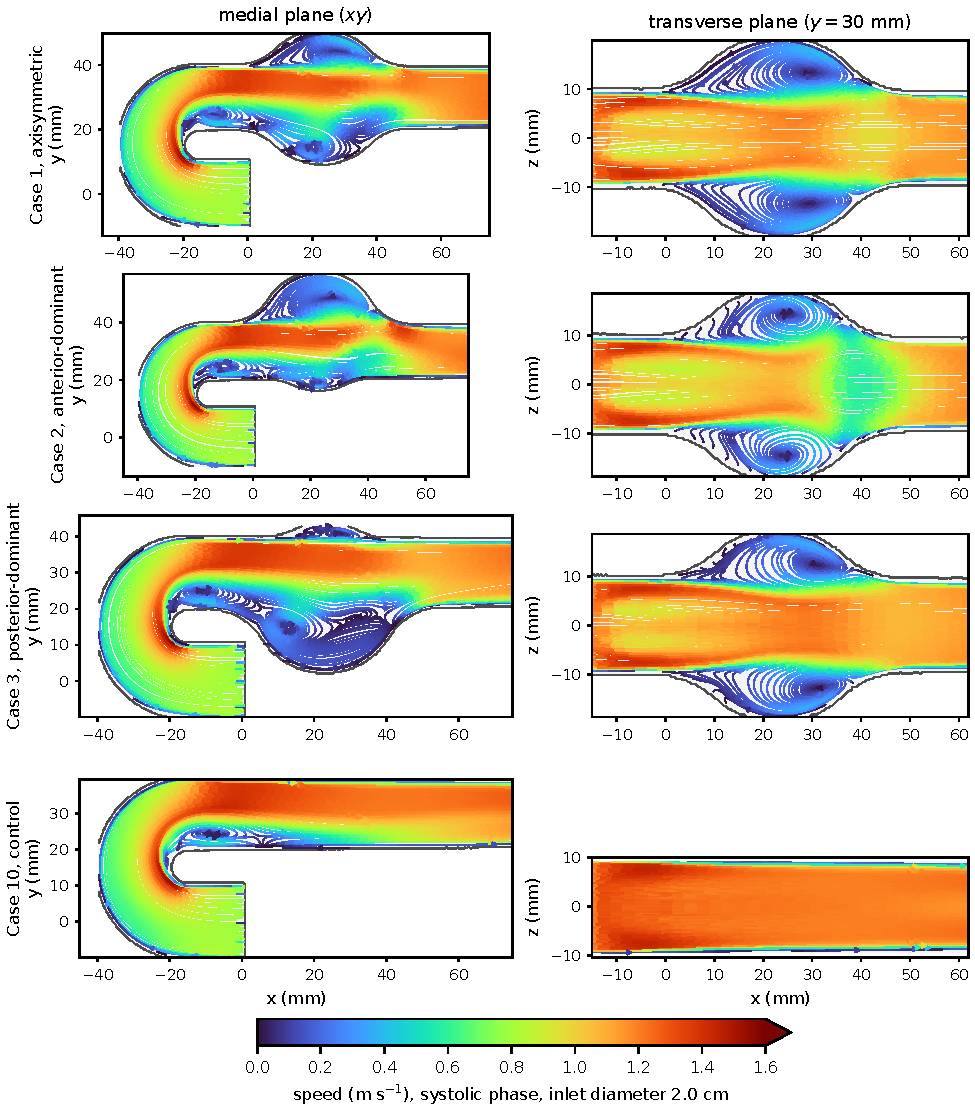
\includegraphics[width=0.92\textwidth]{streamlines_2p0.pdf}
\caption{Streamlines in the systolic phase for the 2.0~cm geometries in the medial plane (left) and the transverse plane (right), colored by in-plane speed on one scale for all geometries. Rows are the axisymmetric, anterior-dominant and posterior-dominant sacs and the control.}
\label{fig:streamlines_2p0}
\end{figure}

\begin{figure}[p]
\centering
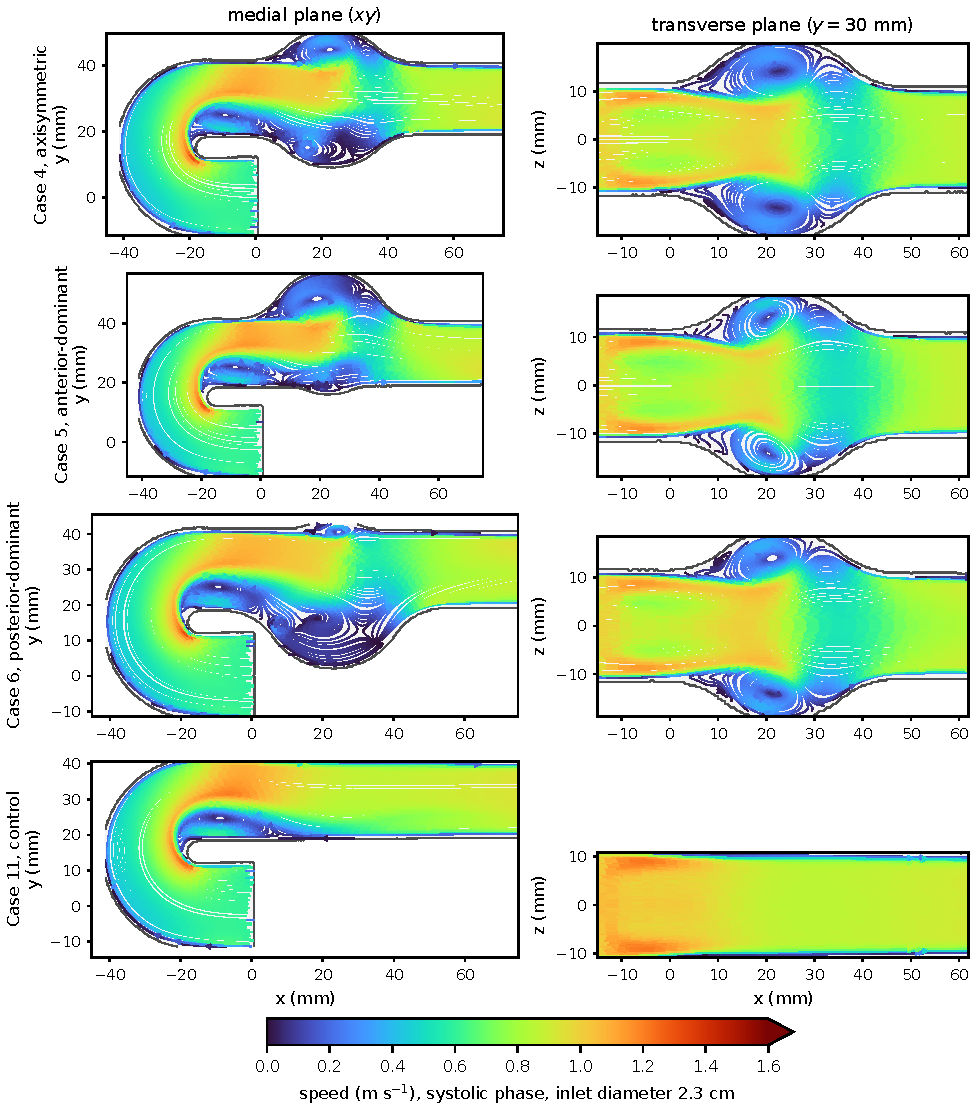
\includegraphics[width=0.92\textwidth]{streamlines_2p3.pdf}
\caption{As Figure~\ref{fig:streamlines_2p0}, for the 2.3~cm geometries.}
\label{fig:streamlines_2p3}
\end{figure}

\begin{figure}[p]
\centering
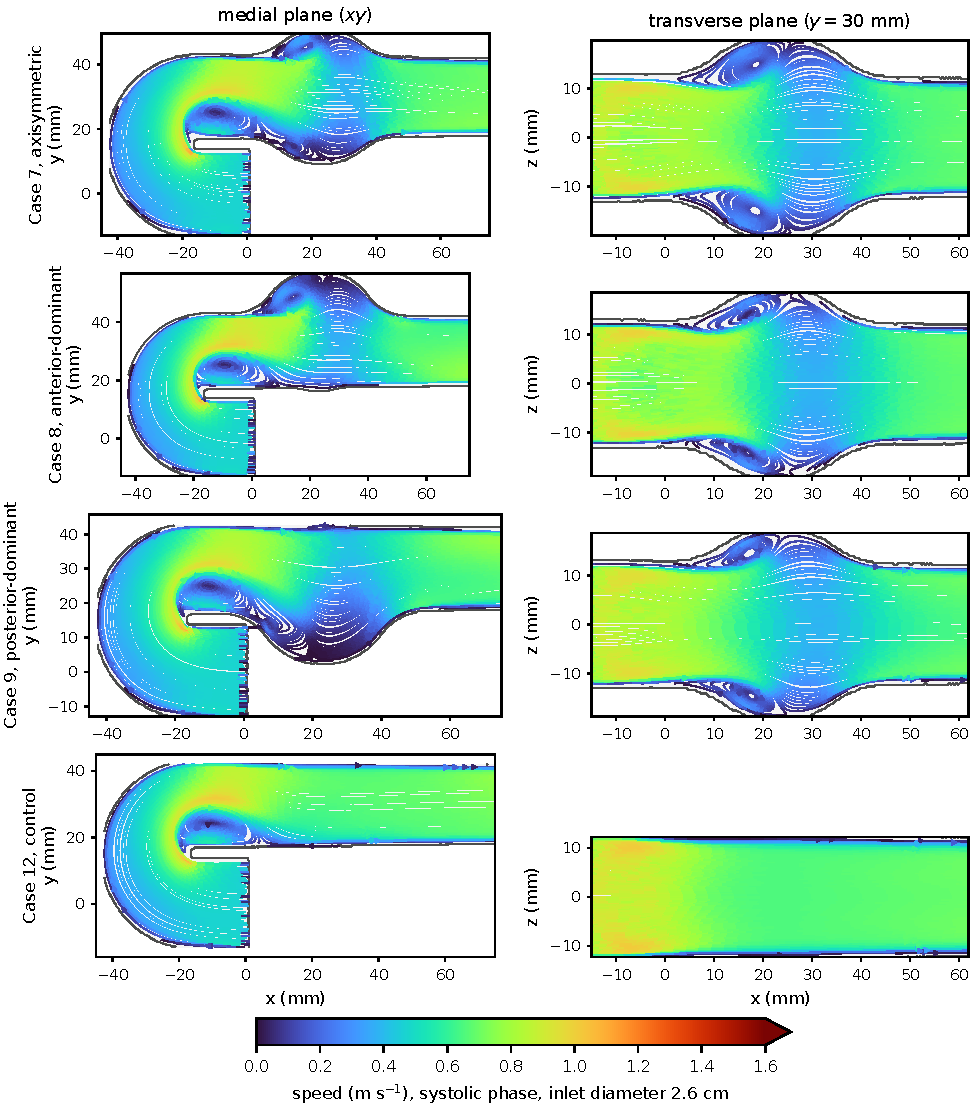
\includegraphics[width=0.92\textwidth]{streamlines_2p6.pdf}
\caption{As Figure~\ref{fig:streamlines_2p0}, for the 2.6~cm geometries.}
\label{fig:streamlines_2p6}
\end{figure}


\subsection{Pressure drop, reversed flow and eddy viscosity}
Table~\ref{tab:cfd_summary} summarizes the common-time flow descriptors for all twelve geometries, and inlet diameter clearly dominates the systolic response. The inlet-to-outlet pressure drop in the systolic phase decreases from \(1261\)--\(1346\,\mathrm{Pa}\) at \(2.0\,\mathrm{cm}\) to \(844\)--\(870\,\mathrm{Pa}\) at \(2.3\,\mathrm{cm}\) and \(528\)--\(561\,\mathrm{Pa}\) at \(2.6\,\mathrm{cm}\), whereas at a fixed diameter the three bulge patterns differ by at most \(7\%\). Relative to the matched control, the dilation adds \(17\)--\(30\%\) to the pressure drop. The fraction of dilation-segment nodes exhibiting reversed axial velocity at systole follows the same ordering, falling from \(50\)--\(54\%\) at \(2.0\,\mathrm{cm}\) to \(38\)--\(40\%\) at \(2.3\,\mathrm{cm}\) and \(24\)--\(28\%\) at \(2.6\,\mathrm{cm}\), against only \(2\)--\(3\%\) in the controls. The mean eddy viscosity within the segment is \(8.6\)--\(9.5\) times the molecular viscosity at \(2.0\,\mathrm{cm}\) but only \(1.6\)--\(2.1\) times at \(2.6\,\mathrm{cm}\). A narrower parent vessel therefore delivers a faster jet into the same \(4.0\,\mathrm{cm}\) sac, producing a larger expansion, a greater fraction of reversed flow, and stronger modeled turbulent mixing. At diastole, by contrast, the pressure drops are only \(1.6\)--\(10.7\,\mathrm{Pa}\), and \(35\)--\(47\%\) of the segment carries reversed flow in every geometry, including the controls, because the slow plateau flow no longer possesses a coherent core.

% Generated by generate_cfd_summary.py from data/processed/full (rigid-wall CFD); CSV: report/tables/eacfm_cfd_summary.csv
\begin{table}[htbp]
\centering
\small
\setlength{\tabcolsep}{3.2pt}
\caption{Common-time descriptors of the rigid-wall \CFD at systole (1.780~s) and
diastole (2.400~s). $\Delta p$ is the difference between the mean static pressure
on the inlet and outlet faces, and the reversed-flow fraction is the fraction of
nodes with $u_x<0$, the local downstream direction in the straight segment. The
evaluation segment is the dilation segment of Section~\ref{sec:exports}; all values
are node-weighted descriptive summaries of single designed geometries.}
\label{tab:cfd_summary}
\resizebox{\textwidth}{!}{%
\begin{tabular}{ccc rr cc cc c cc c}
\toprule
 & & & \multicolumn{2}{c}{$\Delta p$ (Pa)} & \multicolumn{2}{c}{Systolic $\tau_w$ (Pa)} & \multicolumn{2}{c}{Diastolic $\tau_w$ (Pa)} & Mean speed & \multicolumn{2}{c}{Reversed flow (\%)} & $\overline{\mu_t}/\mu$ \\
\cmidrule(lr){4-5}\cmidrule(lr){6-7}\cmidrule(lr){8-9}\cmidrule(lr){11-12}
Case & $D_{\rm in}$ (cm) & $\beta$ & Sys. & Dia. & Median & 95th pct. & Median & 95th pct. & sys. (m~s$^{-1}$) & Sys. & Dia. & sys. \\
\midrule
1 & 2.0 & 1.00 & 1261 & 10.7 & 1.94 & 17.6 & 0.279 & 0.60 & 0.362 & 50 & 35 & 9.5 \\
2 & 2.0 & 0.48 & 1346 & 3.1 & 2.83 & 17.4 & 0.729 & 1.07 & 0.391 & 50 & 45 & 9.4 \\
3 & 2.0 & 2.08 & 1297 & 5.7 & 1.65 & 15.4 & 0.851 & 1.24 & 0.346 & 54 & 45 & 8.6 \\
4 & 2.3 & 1.00 & 844 & 6.8 & 2.30 & 11.7 & 0.253 & 0.46 & 0.328 & 39 & 37 & 3.6 \\
5 & 2.3 & 0.48 & 870 & 1.7 & 2.39 & 10.7 & 0.613 & 0.98 & 0.330 & 38 & 46 & 4.0 \\
6 & 2.3 & 2.08 & 870 & 7.0 & 2.06 & 10.8 & 0.486 & 0.89 & 0.316 & 40 & 43 & 3.2 \\
7 & 2.6 & 1.00 & 545 & 4.9 & 1.87 & 8.1 & 0.251 & 0.59 & 0.275 & 28 & 38 & 1.6 \\
8 & 2.6 & 0.48 & 561 & 1.6 & 1.85 & 7.4 & 0.515 & 0.83 & 0.274 & 28 & 46 & 2.0 \\
9 & 2.6 & 2.08 & 528 & 5.8 & 1.82 & 7.1 & 0.447 & 0.91 & 0.261 & 24 & 47 & 2.1 \\
10 & 2.0 & Control & 1074 & 6.6 & 5.02 & 8.8 & 0.125 & 0.52 & 0.730 & 2 & 35 & 4.2 \\
11 & 2.3 & Control & 668 & 2.8 & 3.53 & 4.9 & 0.103 & 0.38 & 0.546 & 3 & 41 & 2.6 \\
12 & 2.6 & Control & 448 & 1.7 & 2.65 & 3.5 & 0.172 & 0.30 & 0.434 & 3 & 43 & 2.0 \\
\bottomrule
\end{tabular}%
}
\end{table}


\subsection{Wall shear stress}
Figure~\ref{fig:wss_sys} illustrates the \WSS magnitude over the dilation segment in the systolic phase, unwrapped about the axis of the descending segment. In this representation the anterior wall lies at \(0^\circ\) and the posterior wall at \(\pm180^\circ\), so that the full circumference of the vessel is displayed on a single plane. At systole all aneurysmal cases share a low-shear sac body bounded by high-shear rings at the proximal and distal necks, where the jet enters the sac and reattaches. The median segment \WSS is 1.6--2.8~Pa in the aneurysmal cases against 2.7--5.0~Pa in the controls, whereas the 95th percentile is 1.8--2.4 times that of the matched control (Table~\ref{tab:cfd_summary}). The neck rings weaken with increasing inlet diameter, and the 95th percentile falls from 15--18~Pa at 2.0~cm to 7--8~Pa at 2.6~cm. Asymmetry moves the pattern rather than scaling it. In the anterior-dominant cases the low-shear region is centered on the anterior wall (\(0^\circ\)), whereas in the posterior-dominant cases it is centered on the posterior wall (\(\pm180^\circ\)), so that over the sac body the wall opposite the dominant bulge carries the higher shear. In Case~2 the median sac-body \WSS is 4.5~Pa on the posterior wall against 0.9~Pa on the anterior bulge, and in Case~3 the 95th percentile is 8.4~Pa on the anterior wall against 2.1~Pa on the posterior bulge, with the same ordering in Cases~5, 6 and 9 and nearly equal values in Case~8. This behavior is consistent with the streamlines, which show that the jet crossing the sac impinges on the wall opposite the bulge while the bulge itself is filled by slow recirculating flow. At the distal neck the highest shear lies on the anterior (outer-curvature) side in most cases, irrespective of the bulge direction, because the core leaves the bend along the anterior wall.

Figure~\ref{fig:wss_dia} presents the same \WSS magnitude in the diastolic phase on one color scale per phase. At diastole the effect of asymmetry becomes larger than that of diameter. The median segment \WSS of the asymmetric sacs is 0.45--0.85~Pa, which is 1.8--3.1 times that of the axisymmetric sacs (0.25--0.28~Pa) at every diameter and 2.6--6.8 times that of the controls (0.10--0.17~Pa). On comparison of all cases, the diastolic maps show broad shear over the whole wall of the asymmetric sacs, consistent with a residual vortex that keeps moving along the sac wall during the plateau, whereas the axisymmetric sacs and the controls are close to stagnant. These are instantaneous values at two instants; the cycle-averaged picture is given by the \TAWSS maps in Section~\ref{sec:tawss}.

\begin{figure}[!htb]
\centering
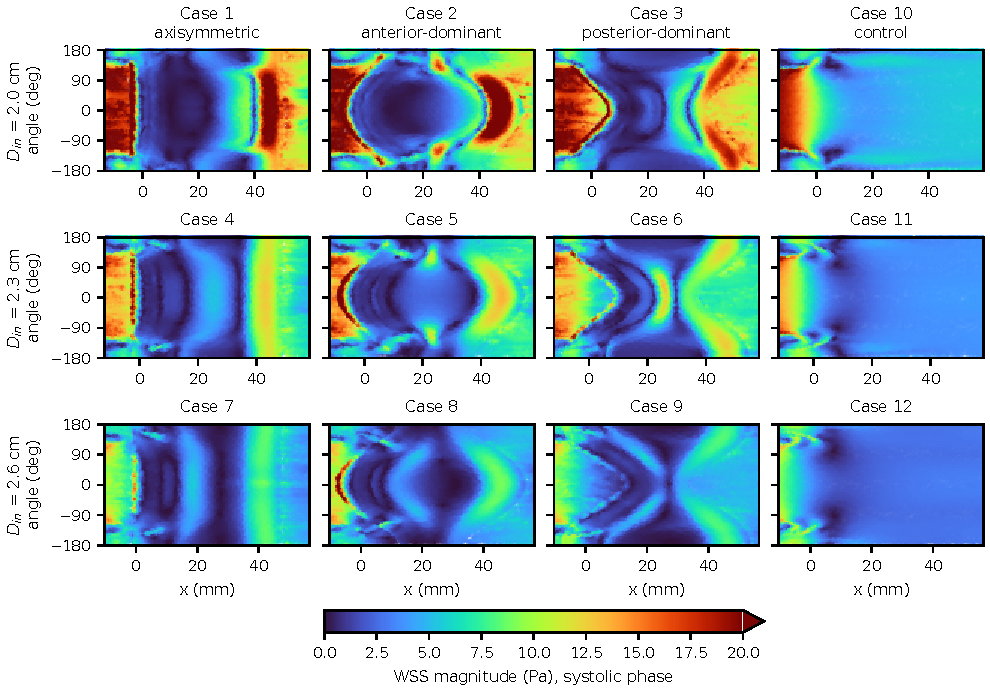
\includegraphics[width=\textwidth]{wss_montage_systole.pdf}
\caption{\WSS magnitude on the dilation segment in the systolic phase, on one color scale saturating at 20~Pa. The wall is unwrapped about the vessel axis, with the anterior wall at \(0^\circ\) and the posterior wall at \(\pm180^\circ\). Rows are inlet diameters and the last column is the matching control. White points are gaps in the exported wall nodes.}
\label{fig:wss_sys}
\end{figure}

\begin{figure}[!htb]
\centering
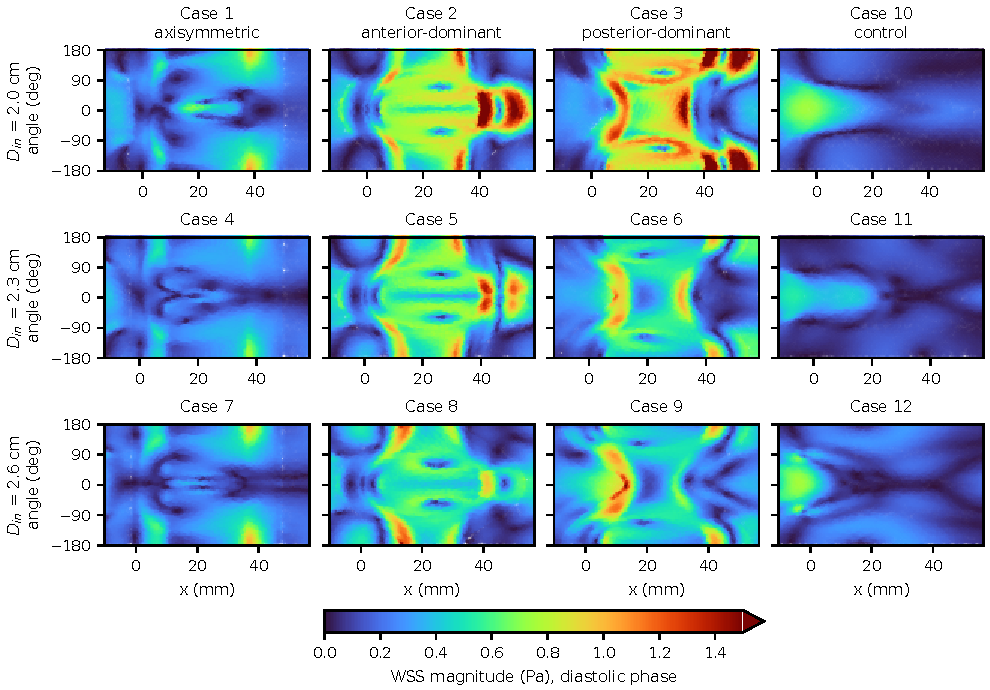
\includegraphics[width=\textwidth]{wss_montage_diastole.pdf}
\caption{As Figure~\ref{fig:wss_sys}, in the diastolic phase, with one color scale saturating at 1.5~Pa.}
\label{fig:wss_dia}
\end{figure}

Figure~\ref{fig:xwss} illustrates the 2D graphics of \WSS for both the medial and transverse planes. Figure~\ref{fig:xwss}(a) represents the \WSS on the anterior wall of the medial plane while Figure~\ref{fig:xwss}(b) shows the \WSS on the posterior wall of the medial plane. Figure~\ref{fig:xwss}(c) presents the \WSS for the transverse plane. Because the aorta bends, a negative value alone does not prove local reverse flow in the curved segment, but along the straight descending segment the negative regions coincide with the recirculation seen in Figures~\ref{fig:streamlines_2p0}--\ref{fig:streamlines_2p6}. On the anterior medial wall and on the transverse wall, \WSS is large and positive at the proximal neck in every case. It becomes negative where the flow detaches on entering the sac, between \(x\approx-4\) and 16~mm on the anterior wall and between 0 and 4~mm on the transverse wall, and it stays negative over the recirculating part of the sac. It returns to positive values, marking reattachment of the core flow, between \(x\approx27\) and 42~mm on the anterior wall and between 26 and 39~mm on the transverse wall, followed by the high positive values of the distal neck. The reattachment point moves upstream as the inlet diameter increases, from 34--42~mm at 2.0~cm to 27--31~mm at 2.6~cm on the anterior wall and from 36--39~mm to 26--27~mm on the transverse wall, so the recirculation region shortens with a wider parent vessel, in line with the reversed-flow fractions of Table~\ref{tab:cfd_summary}. The posterior medial wall differs because \WSS is already negative at the proximal neck in every geometry, the controls included, which identifies this region as the \ICRZ rather than as part of the sac recirculation. The depth of the negative region does not follow the bulge pattern consistently; the most negative value inside the sac, \(-11.3\)~Pa, occurs on the anterior wall of Case~6.

\begin{figure}[!htb]
\centering
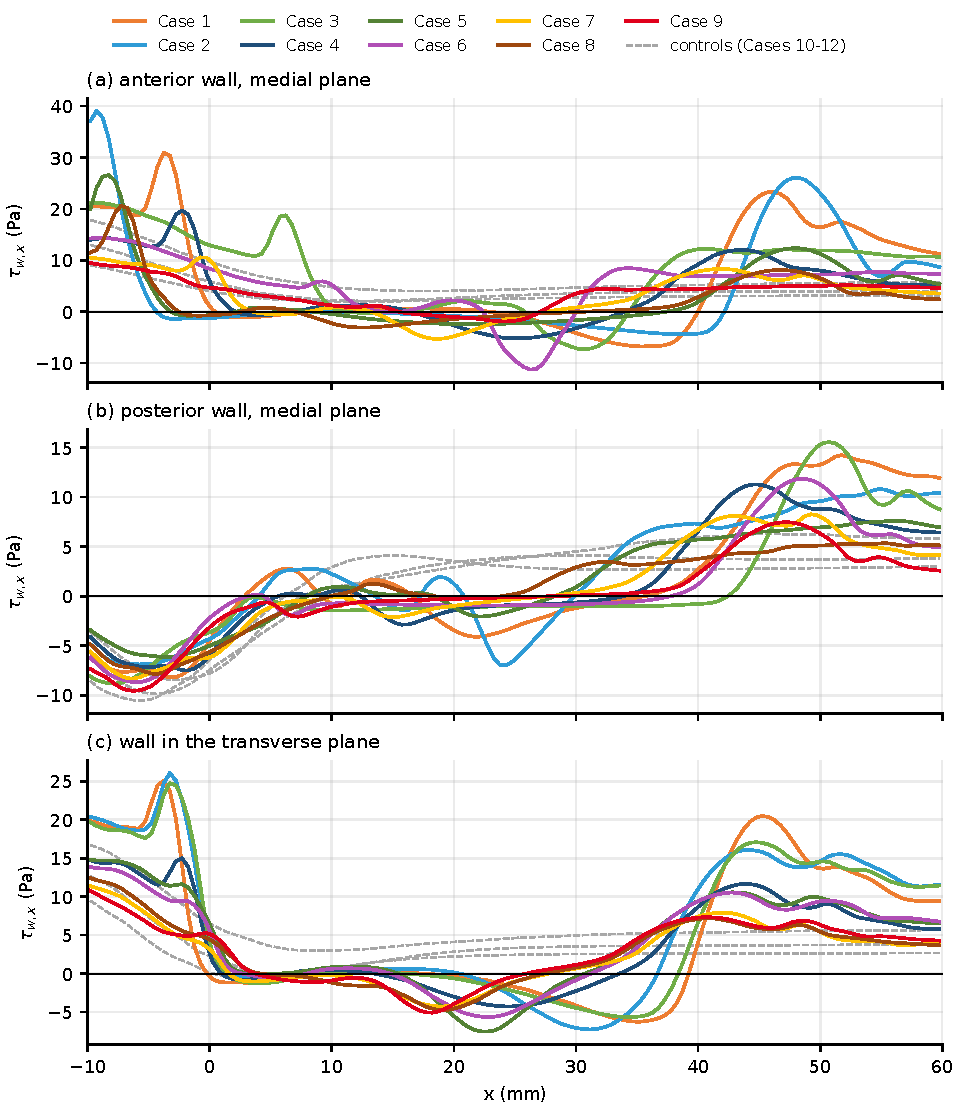
\includegraphics[width=0.85\textwidth]{xwss_lines.pdf}
\caption{2D graphics of \WSS (Pa) in the medial and transverse planes at systolic phase: (a) anterior side of the medial plane, (b) posterior side of the medial plane, and (c) transverse plane.}
\label{fig:xwss}
\end{figure}

\subsection{Time-averaged wall shear stress}
\label{sec:tawss}

The analysis of \TAWSS, as presented in Figure~\ref{fig:tawss} and Table~\ref{tab:tawss}, across twelve idealized geometries revealed several consistent trends. The \TAWSS is shown on the dilation segment of every geometry, unwrapped as in Figure~\ref{fig:wss_sys} and drawn on one logarithmic color scale because the values span two orders of magnitude. Every aneurysmal sac carries a broad region of low \TAWSS. The median over the dilation segment is 0.51--0.83~Pa in the aneurysmal cases against 2.5--4.5~Pa over the same stretch of the controls, while over the sac body the median on either side is 0.23--0.84~Pa. Relative to the matched control, the segment median is lower by a factor of 8.5--8.9 at 2.0~cm, 4.0--4.9 at 2.3~cm and 3.4--3.6 at 2.6~cm, so that the reduction in cycle-averaged shear caused by the dilation is largest for the narrowest parent vessel. Increasing the inlet diameter from 2~cm to 2.6~cm was associated with a progressive reduction in \TAWSS. The high-shear rings at the necks persist in the cycle average, and their strength falls with inlet diameter, the 95th percentile decreasing from 7.6--10.9~Pa at 2.0~cm to 5.5--6.4~Pa at 2.3~cm and 4.1--5.1~Pa at 2.6~cm.

Aneurysm asymmetry had a strong influence on the spatial distribution of \TAWSS. In asymmetric models, the lowest \TAWSS is consistently placed on the dominant bulge. In the anterior-dominant Cases~2, 5 and 8 the sac-body median is 0.34, 0.23 and 0.33~Pa on the anterior wall against 0.52, 0.58 and 0.84~Pa on the posterior wall, whereas in the posterior-dominant Cases~6 and 9 it is 0.24 and 0.28~Pa on the posterior wall against 0.71 and 0.60~Pa on the anterior wall. Case~3 is the exception, with similar values on both sides (0.35 and 0.42~Pa). In the axisymmetric sacs the low-shear region forms circumferential bands with nearly equal anterior and posterior medians. It is also observed that the bulge side is where the instantaneous shear is lowest at systole, so that the dominant bulge is exposed to low shear over the whole cycle rather than at a single instant. This reinforces the need for a multi-parametric hemodynamic assessment that includes both \WSS and \TAWSS to identify rupture-prone \DTAAs. Low \TAWSS, in particular, marks regions of prolonged low shear, which are known to promote thrombus formation~\cite{salman2019biomechanical}, although the present models do not include those processes.

\begin{figure}[!htb]
\centering
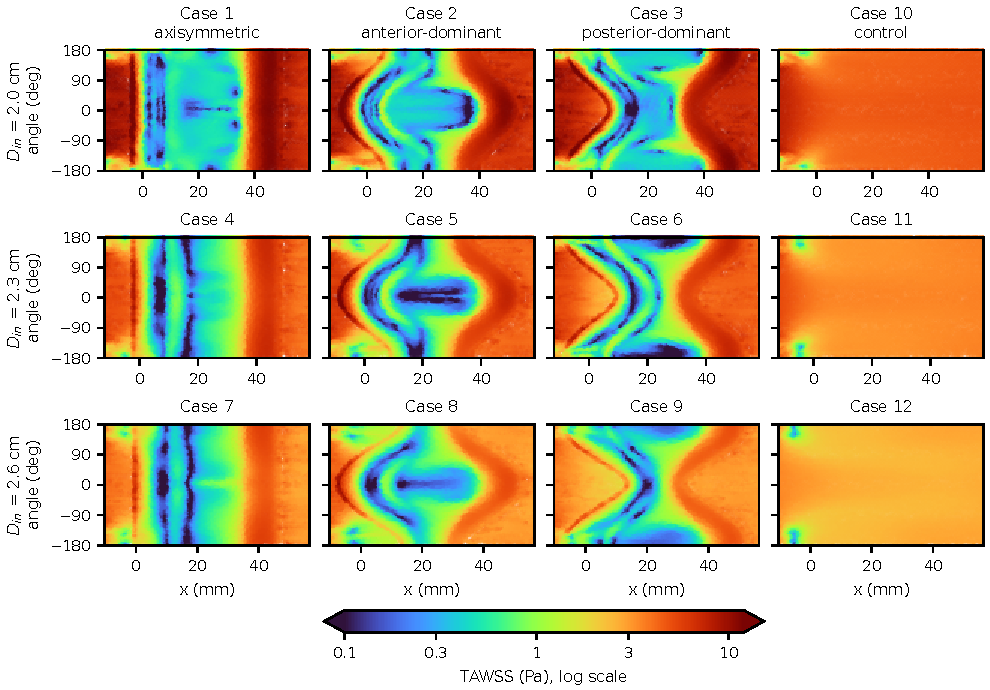
\includegraphics[width=\textwidth]{tawss_montage.pdf}
\caption{\TAWSScap on the dilation segment, unwrapped as in Figure~\ref{fig:wss_sys}, on one logarithmic color scale. Rows are inlet diameters and the last column is the matching control.}
\label{fig:tawss}
\end{figure}

% Generated by scripts/manuscript/generate_wss_montage.py from data/raw/TAWSS 30.09.2026.
\begin{table}[htbp]
\centering
\small
\caption{\revision{TAWSS (Pa) on the dilation segment. Percentiles are over the whole segment, while the sac-body medians use its middle third, within $60^\circ$ of the anterior or posterior direction.}}
\label{tab:tawss}
\begin{tabular}{cclccccc}
\toprule
 & & & \multicolumn{3}{c}{Segment} & \multicolumn{2}{c}{Sac body, median} \\
\cmidrule(lr){4-6}\cmidrule(lr){7-8}
Case & $D_{\rm in}$ (cm) & Morphology & 5th pct. & Median & 95th pct. & Anterior & Posterior \\
\midrule
1 & 2.0 & axisymmetric & 0.19 & 0.51 & 10.86 & 0.41 & 0.47 \\
2 & 2.0 & anterior-dominant & 0.15 & 0.52 & 7.60 & 0.34 & 0.52 \\
3 & 2.0 & posterior-dominant & 0.18 & 0.53 & 8.66 & 0.35 & 0.42 \\
10 & 2.0 & control & 3.65 & 4.53 & 4.89 & 4.66 & 4.36 \\
4 & 2.3 & axisymmetric & 0.12 & 0.70 & 6.41 & 0.47 & 0.49 \\
5 & 2.3 & anterior-dominant & 0.10 & 0.67 & 5.45 & 0.23 & 0.58 \\
6 & 2.3 & posterior-dominant & 0.10 & 0.83 & 5.82 & 0.71 & 0.24 \\
11 & 2.3 & control & 2.81 & 3.30 & 3.52 & 3.45 & 3.20 \\
7 & 2.6 & axisymmetric & 0.12 & 0.70 & 5.06 & 0.45 & 0.50 \\
8 & 2.6 & anterior-dominant & 0.17 & 0.73 & 4.12 & 0.33 & 0.84 \\
9 & 2.6 & posterior-dominant & 0.18 & 0.69 & 4.24 & 0.60 & 0.28 \\
12 & 2.6 & control & 2.20 & 2.51 & 2.82 & 2.59 & 2.51 \\
\bottomrule
\end{tabular}
\end{table}


\FloatBarrier

\subsection{Structural wall stress}
\label{sec:structural}

It is widely recognized that aneurysm rupture risk is associated with maximum diameter; however, this relationship is not absolute. Darling et al.~\cite{darling1977autopsy} observed that some large aneurysms do not rupture, whereas smaller ones do, indicating that additional factors such as aneurysm geometry and asymmetry play a critical role. Aneurysm rupture occurs when the mechanical load exceeds the tissue strength of the arterial wall, and understanding this mechanical mechanism is essential for assessing rupture risk in \DTAA. Our results indicate that aneurysm shape and inlet diameter markedly change the modeled wall-stress distribution. Previous studies, including those by Dobrin~\cite{dobrin1989pathophysiology}, have applied Laplace's law to estimate wall stress. However, Laplace's law predicts the greatest wall stress at the maximum bulge of the aneurysm sac, which is not consistent with the biomechanical behavior observed in aneurysmal geometries. As demonstrated in the present study, the stress distribution within the aneurysm wall is governed by asymmetry and geometric features.

Figure~\ref{fig:mps} presents the \MPS on the inner surface of the wall over the dilation segment, unwrapped as in Figure~\ref{fig:wss_sys}, and Table~\ref{tab:mps} summarizes it. In every aneurysmal case the \MPS is highest in circumferential bands at the necks, where the wall curvature changes sign, with 95th percentiles of 101--113~kPa over the necks, and lowest over the crown of the sac, where the medians are 55--80~kPa. This pattern is consistent with the findings of Vorp et al.~\cite{vorp1998mechanical}. A clear distinction was observed between axisymmetric and asymmetric cases. In the axisymmetric models, the stress was elevated at the proximal regions but lower at the midsection of the aneurysm sac, with similar behavior on both anterior and posterior sides; the anterior and posterior sac-body medians are equal to within 1~kPa. In contrast, the asymmetric models exhibited higher stress on the side opposite to the dominant bulge. The sac-body median on the posterior wall of the anterior-dominant Cases~2, 5 and 8 is 69.2, 73.6 and 78.1~kPa against 55.9, 55.0 and 61.8~kPa on the anterior bulge, and the anterior wall of the posterior-dominant Cases~3, 6 and 9 carries 68.3, 72.9 and 80.3~kPa against 55.8, 55.3 and 57.2~kPa on the posterior bulge. The opposite-side value increases with inlet diameter, as does the segment median of the controls (52.5, 58.4 and 65.1~kPa), because the loaded radius grows with the parent vessel.

In contrast, the healthy cases (10--12) exhibited relatively uniform wall stress distributions, with 95th percentiles within 3~kPa of their medians and only mild elevations at the bend. Compared to the diseased cases, where stress varied non-uniformly due to the presence of the aneurysm, the healthy aortas showed more consistent stress profiles. Assuming uniform wall strength, these results indicate that the side opposite to the dominant bulge is at a higher risk of rupture compared to the other side. Among the six asymmetric cases, the highest \MPS was observed in Case~9 on the anterior side, so that, if the wall strength were the same on both sides, this site would carry the highest modeled stress of all sides and cases. With a uniform 2~mm wall, literature material parameters, fixed ends and a quasi-static coupling whose step settings were not retained, the stress magnitudes indicate where the modeled wall is most loaded rather than where it would fail, since failure also depends on the unknown local wall strength.

\begin{figure}[!htb]
\centering
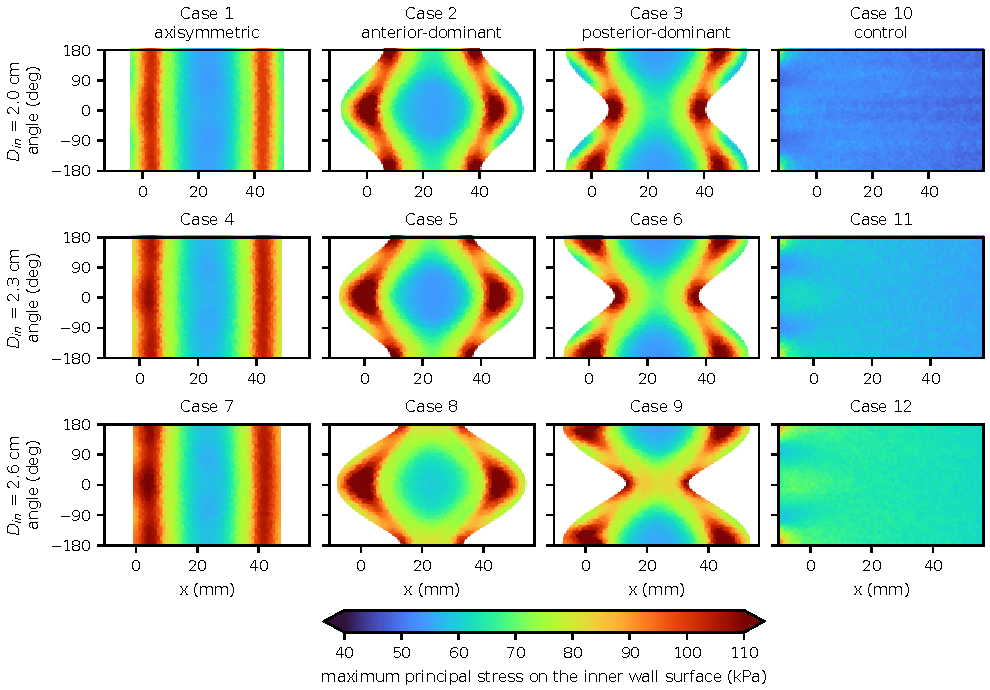
\includegraphics[width=\textwidth]{mps_montage.pdf}
\caption{\MPScap on the inner wall surface of the dilation segment, unwrapped as in Figure~\ref{fig:wss_sys}, on one color scale. Rows are inlet diameters and the last column is the matching control.}
\label{fig:mps}
\end{figure}

% Recomputed 2026-10-16 from data/raw/MPS; Case 8 uses the replacement data/Case 8.xls.
\begin{table}[htbp]
\centering
\small
\caption{\revision{Maximum principal stress (kPa) on the inner wall surface of the dilation segment. Sac-body medians use the middle third of the segment, within $60^\circ$ of the anterior or posterior direction, while the neck value is the 95th percentile over the outer thirds.}}
\label{tab:mps}
\begin{tabular}{cclccccc}
\toprule
 & & & \multicolumn{2}{c}{Segment} & \multicolumn{2}{c}{Sac body, median} & Necks \\
\cmidrule(lr){4-5}\cmidrule(lr){6-7}\cmidrule(lr){8-8}
Case & $D_{\rm in}$ (cm) & Morphology & Median & 95th pct. & Anterior & Posterior & 95th pct. \\
\midrule
1 & 2.0 & axisymmetric & 67.6 & 99.5 & 56.7 & 56.7 & 101.0 \\
2 & 2.0 & anterior-dominant & 70.2 & 106.9 & 55.9 & 69.2 & 111.3 \\
3 & 2.0 & posterior-dominant & 69.8 & 105.5 & 68.3 & 55.8 & 110.0 \\
10 & 2.0 & control & 52.5 & 54.8 & 52.4 & 52.8 & 54.9 \\
4 & 2.3 & axisymmetric & 71.4 & 103.9 & 58.1 & 59.0 & 104.5 \\
5 & 2.3 & anterior-dominant & 72.4 & 108.5 & 55.0 & 73.6 & 113.4 \\
6 & 2.3 & posterior-dominant & 72.2 & 107.4 & 72.9 & 55.3 & 112.1 \\
11 & 2.3 & control & 58.4 & 60.7 & 58.7 & 58.9 & 61.0 \\
7 & 2.6 & axisymmetric & 74.1 & 105.2 & 59.4 & 60.6 & 106.3 \\
8 & 2.6 & anterior-dominant & 75.9 & 111.6 & 55.3 & 80.5 & 117.7 \\
9 & 2.6 & posterior-dominant & 76.5 & 107.3 & 80.3 & 57.2 & 112.9 \\
12 & 2.6 & control & 65.1 & 67.6 & 65.3 & 65.7 & 68.0 \\
\bottomrule
\end{tabular}
\end{table}


\FloatBarrier

\subsection{Plane-wise flow summaries}
\label{sec:planes}

In addition to the wall-based hemodynamic and biomechanical indices, a plane-wise cross-sectional analysis was performed to quantify the spatial variation of flow features along the aorta. Velocity and \TKE were evaluated at selected axial planes to identify the regions where aneurysm morphology most strongly altered the flow field. This approach allows the three-dimensional flow disturbance to be reduced into comparable regional quantities from the proximal to distal sections of the vessel.

The locations of the eight planes are shown in Figure~\ref{fig:diagram} and the details of aortic diameter are available in Table~\ref{tab:diameter}. All models incorporated a taper ratio of 0.8 from inlet to outlet, a physiologically important feature that gradually reduces the vessel diameter distally, thereby maintaining flow momentum and regulating perfusion to downstream vessels. Figure~\ref{fig:planes} shows the plane-averaged speed and \TKE of every case from the retained slice summaries, and Table~\ref{tab:plane_cfd} gives the medians of the aneurysmal and control groups. The taper is visible in every model, with the speed at D7 and D8 above that at D1--D3 because the lumen narrows toward the outlet. This tapering-induced acceleration is essential for maintaining adequate perfusion pressure that ensures sufficient blood flow to downstream vascular beds. Indeed, studies have shown that flow velocity increases while vessel diameter decreases~\cite{kahveci2015numerical}. In the aneurysmal cases the speed falls sharply across the sac to 0.10--0.16~m~s$^{-1}$ at D5, where the lumen diameter is 4.0~cm whatever the inlet diameter, against a median of 0.193~m~s$^{-1}$ in the controls, and it recovers by D7. This is a direct consequence of the local dilation, where the increased cross-sectional area reduces flow velocity to conserve mass.

In contrast to velocity, the modeled $k$ as shown in Figure~\ref{fig:planes} rises through the sac, peaks at D5 at about twice the control value, remains elevated at D6 and D7, where the jet reattaches and the recirculation of the distal sac develops, and returns to the control level by D8. At plane~5 (the maximum diameter of the bulge, the center of the aneurysm sac), strong flow separation and recirculation zones produce high $k$. At plane~6 (distal sac) and plane~7 (post-aneurysm), $k$ remains elevated, implying that the disturbed flow persists downstream of the aneurysm sac. This pattern is consistent with the fact that recirculation zones predominantly appear on the distal side of the aneurysm, where the flow jet impinges and vortices develop~\cite{yu2000steady}. Conversely, at D4, the proximal neck, the aneurysmal and control values still overlap, so the turbulent disturbance is generated inside the sac rather than at its entrance, and it decays within about one sac length downstream. Thus, $k$ only rises sharply once the flow reaches the central and distal portions of the sac, where recirculation becomes fully established. By plane~8 (near the outlet), the $k$ has returned to the control level, demonstrating that the turbulence has largely dissipated before reaching the distal boundary. The asymmetric sacs reach higher $k$ at D5 than the axisymmetric ones at every diameter.

Overall, the plane-wise analysis confirms that the aneurysm-induced flow disturbance is highly localized rather than uniformly distributed along the entire aorta. The velocity results identified the strongest reduction at plane~5, corresponding to the maximum aneurysm diameter, whereas the $k$ results showed that disturbed and vortical flow persists from the aneurysm center to the distal sac and post-aneurysm region. Thus, the plane-based quantities provide complementary information to the wall-based indices. While \WSS and \TAWSS describe near-wall hemodynamic loading and \MPS describes structural wall stress, the plane-wise velocity and $k$ analysis captures the intraluminal flow disturbance and its downstream propagation. Therefore, the plane-wise analysis provides quantitative evidence that the maximum aneurysm diameter primarily reduces local velocity, whereas aneurysm morphology and sac expansion generate elevated \TKE over a broader downstream region.

\begin{figure}[!htb]
\centering
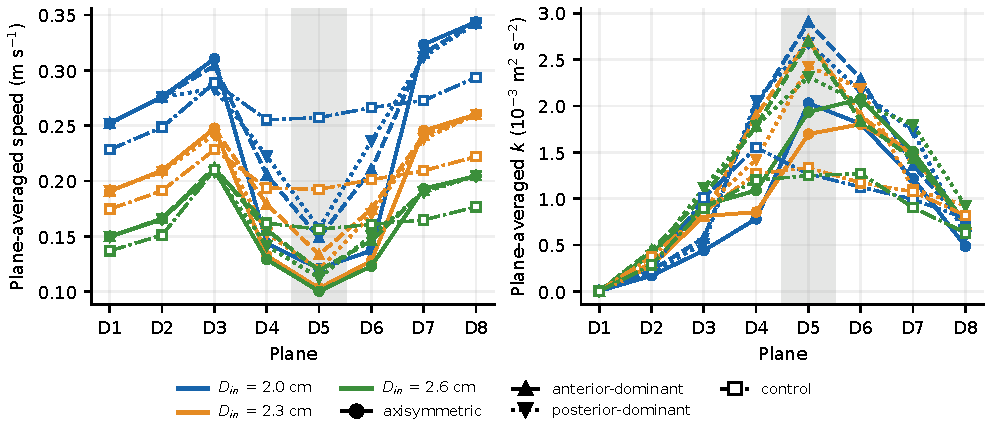
\includegraphics[width=\textwidth]{plane_profiles.pdf}
\caption{Plane-averaged speed (left) and \TKE per unit mass (right) at D1--D8 for all twelve geometries. Color gives the inlet diameter, and line style and marker the morphology; controls are dash-dot with open squares. The band marks the sac center (D5).}
\label{fig:planes}
\end{figure}

% Generated from corrected data/results_on_slices.csv on 2026-09-27.
\begin{table}[htbp]
\centering
\caption{Descriptive medians of the reported plane-averaged CFD quantities across nine aneurysmal and three control geometries. $k$ is turbulent kinetic energy per unit mass (m$^2$~s$^{-2}$). These designed cases do not support patient-population significance tests.}
\label{tab:plane_cfd}
\begin{tabular}{lcccc}
\toprule
& \multicolumn{2}{c}{Mean speed (m~s$^{-1}$)} & \multicolumn{2}{c}{$k$ ($10^{-3}$ m$^2$~s$^{-2}$)} \\
Plane & Aneurysmal & Control & Aneurysmal & Control \\
\midrule
D1 & 0.191 & 0.175 & 0.002 & 0.003 \\
D2 & 0.209 & 0.191 & 0.275 & 0.287 \\
D3 & 0.247 & 0.228 & 0.815 & 0.896 \\
D4 & 0.153 & 0.194 & 1.783 & 1.270 \\
D5 & 0.120 & 0.193 & 2.425 & 1.266 \\
D6 & 0.151 & 0.201 & 2.028 & 1.171 \\
D7 & 0.241 & 0.209 & 1.468 & 0.993 \\
D8 & 0.260 & 0.222 & 0.728 & 0.788 \\
\bottomrule
\end{tabular}
\end{table}


\section{Reconstruction results}
\label{sec:reconstruction_results}
\subsection{Checks on the complete \texorpdfstring{\CFD}{CFD} fields}
\label{sec:reference_results}
Before any fitting, the complete \CFD fields of the nine aneurysmal cases were used to check Eq.~\eqref{eq:momentum} and to measure the post-processing floors. With 40-neighbor least-squares gradients, the unsteady form with the \CFD eddy viscosity and without a $2\rho k/3$ term gave the smallest momentum residual in every case and phase, at 0.03--0.17 of the convective term in the bulk of the lumen. Omitting the time derivative raised the residual to 0.18--0.30 of convection at systole, and to 0.45--0.56 inside the sac, and to 0.49--0.73 at diastole, and adding the $2\rho k/3$ term made the residual larger. A quasi-steady momentum residual is therefore not consistent with these transient fields, particularly inside the sac.

Table~\ref{tab:reference_floor} gives the floors obtained by passing the complete \CFD velocity through the shared post-processing. Integrating the \CFD's own pressure gradient reproduces the \CFD pressure to 0.5--0.9\%, so the integration itself is accurate, and the remaining floor comes from the momentum terms. With the unsteady form and oracle $\mu_t$ the pressure floor is 1.6--2.3\% at systole, except for Case~2, whose forward window gives 7.1\%, and 2.2--4.1\% at diastole. Information matters differently in the two phases. At systole the molecular form is almost as good as the oracle for the 2.3 and 2.6~cm cases (1.8--2.7\%) but not for the 2.0~cm cases (4.9--11.3\%), in line with their larger eddy viscosity (Table~\ref{tab:cfd_summary}). At diastole removing either the time term or the eddy viscosity degrades the floor substantially, to 3.9--10.3\% and 9.0--19.3\%, respectively. The \WSS floor depends strongly on the distance $h$ in Eq.~\eqref{eq:wss_estimate}. At systole it is 0.07--0.09 at $h=0.1$~mm but 0.14--0.27 at the prespecified $h=0.25$~mm, because the systolic velocity profile is no longer close to quadratic over the $2h=0.5$~mm stencil, whereas at diastole it is 0.04--0.06 at either distance.

% Generated by generate_reference_table.py from the cfd run records.
\begin{table}[htbp]
\centering
\small
\setlength{\tabcolsep}{4pt}
\caption{\revision{\textcolor{red}{Pipeline floor, obtained by passing the complete CFD velocity through the shared post-processing. Pressure columns give the sub-cloud relative L2 error for each information setting, combining retention or omission of the time term with either CFD eddy viscosity or molecular viscosity alone. $\Delta p_{\rm sub}$ is the CFD pressure drop between the inlet and outlet ends of the sub-cloud. Wall-shear columns give the aneurysm-zone magnitude error of the one-sided estimate at $h=0.1$~mm and at the prespecified $h=0.25$~mm. Case 2's systolic window runs forward from the target (1.780--1.788~s), which explains its larger unsteady error.}}}
\label{tab:reference_floor}
\begin{tabular}{llccccrcc}
\toprule
 & & \multicolumn{4}{c}{Pressure relative L2} & & \multicolumn{2}{c}{Wall shear} \\
\cmidrule(lr){3-6}\cmidrule(lr){8-9}
Case & Phase & Unst.+$\mu_t$ & Steady+$\mu_t$ & Unst.+$\mu$ & Steady+$\mu$ & $\Delta p_{\rm sub}$ (Pa) & $h=0.1$ & $h=0.25$ \\
\midrule
1 & Sys. & 0.022 & 0.031 & 0.049 & 0.067 & 986.1 & 0.086 & 0.249 \\
1 & Dia. & 0.035 & 0.074 & 0.152 & 0.188 & 8.8 & 0.044 & 0.042 \\
2 & Sys. & 0.071 & 0.027 & 0.113 & 0.048 & 1063.4 & 0.090 & 0.273 \\
2 & Dia. & 0.037 & 0.056 & 0.145 & 0.154 & 1.1 & 0.048 & 0.042 \\
3 & Sys. & 0.022 & 0.029 & 0.065 & 0.071 & 1010.2 & 0.090 & 0.220 \\
3 & Dia. & 0.024 & 0.039 & 0.091 & 0.101 & 3.7 & 0.048 & 0.046 \\
4 & Sys. & 0.019 & 0.037 & 0.023 & 0.036 & 664.2 & 0.077 & 0.182 \\
4 & Dia. & 0.032 & 0.103 & 0.175 & 0.242 & 5.5 & 0.050 & 0.037 \\
5 & Sys. & 0.019 & 0.036 & 0.027 & 0.036 & 682.4 & 0.094 & 0.208 \\
5 & Dia. & 0.031 & 0.051 & 0.114 & 0.121 & 0.4 & 0.052 & 0.041 \\
6 & Sys. & 0.018 & 0.033 & 0.026 & 0.032 & 685.4 & 0.078 & 0.191 \\
6 & Dia. & 0.041 & 0.068 & 0.193 & 0.211 & 5.8 & 0.054 & 0.042 \\
7 & Sys. & 0.016 & 0.037 & 0.018 & 0.035 & 412.8 & 0.070 & 0.151 \\
7 & Dia. & 0.038 & 0.090 & 0.172 & 0.246 & 4.1 & 0.050 & 0.040 \\
8 & Sys. & 0.023 & 0.048 & 0.018 & 0.042 & 422.4 & 0.090 & 0.183 \\
8 & Dia. & 0.039 & 0.065 & 0.154 & 0.160 & 0.6 & 0.055 & 0.043 \\
9 & Sys. & 0.020 & 0.033 & 0.020 & 0.033 & 397.3 & 0.070 & 0.141 \\
9 & Dia. & 0.022 & 0.045 & 0.090 & 0.096 & 4.8 & 0.060 & 0.048 \\
\bottomrule
\end{tabular}
\end{table}


\subsection{Momentum-constrained \texorpdfstring{\PINNs}{PINNs} on the development geometries}
\label{sec:pilot_results}
In the development cases, every neural field reconstructed the hidden velocity three to four times more accurately than \RBF (relative errors 0.037--0.052 versus 0.13--0.16 at systole) and five times more accurately than linear interpolation. However, the prespecified criterion of the development test failed on both endpoints (Table~\ref{tab:pilot}). The momentum arms were trained with a blood density of 1060~kg~m$^{-3}$ in the scaling of their residual before the density was corrected to 1050~kg~m$^{-3}$; all reported scores use the corrected value, and the 1\% difference in the residual scaling does not affect the conclusions drawn from them. The gate scored the momentum \PINNs by their own pressure output and automatic-differentiation \WSS, the direct route that a \PINN offers, and the other methods by shared post-processing, so the comparison changes both the fitting and the pressure route. The unsteady \PINN's own pressure output had errors of 0.43--0.53 at systole and 0.56--1.05 at diastole, and the steady \PINN's 0.51--0.90, whereas the continuity field passed through the shared integration reached 0.023--0.049. The \PINN's automatic-differentiation \WSS (0.40--0.45 at systole) was also worse than the pipeline \WSS of the continuity field (0.35--0.37).

Because the gate changed both the fitting and the pressure route, we also passed the velocity of every momentum \PINN through the shared post-processing (Table~\ref{tab:pilot_pipeline}). In the prespecified unsteady form the unsteady \PINN's velocity still gave pressure errors of 0.37--0.48 at systole and 0.58--1.11 at diastole, against 0.023--0.049 for the continuity field, because that form uses the difference between the field's two snapshots. Dropping the time term reduced the error to 0.037--0.089, still above the continuity field. The \PINN's momentum residual was an order of magnitude smaller than that of the continuity field (0.2 against 2.5 in scaled units), so the network satisfied the momentum balance by adjusting a time derivative that was constrained only at the observed nodes of two snapshots 5--10~ms apart. With so little temporal information, $\partial_t\mathbf u$ and the pressure act as slack variables in a soft momentum penalty rather than as information. The steady \PINN, whose loss does not contain a time derivative, came close to the continuity field only in the systolic window of Case~1 (0.029 against 0.025). For \WSS the shared estimate gave similar errors for all fields at systole (0.34--0.40), and the momentum \PINNs gave lower errors in the diastolic Case~9 window (0.11--0.12 against 0.22). Adding the momentum balance to the loss therefore did not improve the velocity used for pressure, although it helped \WSS in one diastolic window. The confirmation study therefore evaluated the continuity field with physics applied after fitting, as specified in Section~\ref{sec:protocol}.


\begin{table}[htbp]
\centering
\small
\caption{Pilot endpoints. The continuity field is scored through the shared post-processing, and the momentum PINNs through their own pressure output and automatic-differentiation WSS. Values average two draws at systole and one at diastole.}
\label{tab:pilot}
\begin{tabular}{llccccc}
\toprule
Case & Phase & \shortstack{Cont. pressure\\(post-proc.)} & \shortstack{Steady head\\(direct)} & \shortstack{Unsteady head\\(direct)} & \shortstack{Cont. shear\\(post-proc.)} & \shortstack{Unsteady shear\\(autograd)} \\
\midrule
1 & Sys. & 0.025 & 0.787 & 0.435 & 0.369 & 0.447 \\
1 & Dia. & 0.045 & 0.897 & 1.048 & 0.113 & 0.130 \\
9 & Sys. & 0.023 & 0.633 & 0.531 & 0.346 & 0.396 \\
9 & Dia. & 0.049 & 0.515 & 0.558 & 0.224 & 0.155 \\
\bottomrule
\end{tabular}
\end{table}

% Generated by scripts/manuscript/generate_pilot_pipeline.py.
\begin{table}[htbp]
\centering
\small
\caption{Pilot fields scored through the same post-processing. Pressure is the relative L2 error of momentum integration applied to each field's velocity, in the prespecified unsteady form with CFD eddy viscosity, and, for the unsteady PINN, also in the steady form, which does not use the field's time derivative. WSS is the finite-distance estimate at $h=0.25$~mm. All fields use the CFD eddy viscosity. Values are averaged over two draws at systole and one at diastole.}
\label{tab:pilot_pipeline}
\setlength{\tabcolsep}{4pt}
\begin{tabular}{llccccccc}
\toprule
 & & \multicolumn{4}{c}{Pressure} & \multicolumn{3}{c}{Aneurysm-zone WSS} \\
\cmidrule(lr){3-6}\cmidrule(lr){7-9}
Case & Phase & \shortstack{Cont.\\field} & \shortstack{Steady\\PINN} & \shortstack{Unsteady\\PINN} & \shortstack{Unsteady PINN,\\steady form} & \shortstack{Cont.\\field} & \shortstack{Steady\\PINN} & \shortstack{Unsteady\\PINN} \\
\midrule
1 & Sys. & 0.025 & 0.029 & 0.373 & 0.046 & 0.369 & 0.399 & 0.401 \\
1 & Dia. & 0.045 & 0.060 & 1.103 & 0.089 & 0.113 & 0.118 & 0.100 \\
9 & Sys. & 0.023 & 0.036 & 0.479 & 0.037 & 0.346 & 0.347 & 0.335 \\
9 & Dia. & 0.049 & 0.126 & 0.577 & 0.050 & 0.224 & 0.123 & 0.111 \\
\bottomrule
\end{tabular}
\end{table}


\subsection{Confirmation on seven held-out geometries}
\label{sec:confirmation}
At the primary 2.5~mm spacing the continuity field followed by the shared post-processing had lower pressure error than \RBF with the same post-processing in all 14 case--phase units, with a median ratio of 0.458, and lower aneurysm-zone \WSS error in all 14 units, with a median ratio of 0.508 (Table~\ref{tab:recon_summary}, Figure~\ref{fig:confirmation}). Both prespecified hypotheses were met, and the velocity guardrail held in every unit, with hidden-velocity errors of 0.033--0.050 against 0.113--0.169 for \RBF. At the level of individual draws the \WSS advantage held in 42 of 42 comparisons, whereas the pressure advantage held in 39 of 42. The prespecified decision rule was the count of units, and no significance test was planned. For reference, a two-sided sign test on the draw-level comparisons gives $p<10^{-8}$ for both quantities, although draws within a unit share a geometry and are not independent. The three adverse pressure draws were all diastolic, in Case~4 (ratio 1.05), Case~7 (1.40) and Case~8 (1.75), and the case-wise tables in Appendix~\ref{app:casewise} show that the diastolic pressure error of the neural field varies between draws by up to 0.085, several times more than \RBF's.

\begin{table}[htbp]
\centering
\small
\caption{Median of seven case means at 2.5~mm; each reconstructed case mean uses three paired draws. Entries are node-weighted relative L2 errors. Pressure is conditional on oracle CFD eddy viscosity. Full CFD denotes the same post-processing applied to complete velocity; its error is a reference, not a strict lower bound.}
\label{tab:recon_summary}
\begin{tabular}{llccccc}
\toprule
Phase & Quantity & Continuity & Data-only & RBF & Linear & Full CFD \\
\midrule
Systole & Velocity & 0.044 & 0.052 & 0.146 & 0.226 & 0.000 \\
Systole & Pressure & 0.023 & 0.028 & 0.079 & 0.292 & 0.019 \\
Systole & Wall shear & 0.356 & 0.333 & 0.609 & 0.834 & 0.191 \\
Diastole & Velocity & 0.038 & 0.039 & 0.130 & 0.242 & 0.000 \\
Diastole & Pressure & 0.094 & 0.063 & 0.132 & 0.167 & 0.037 \\
Diastole & Wall shear & 0.163 & 0.161 & 0.374 & 0.615 & 0.042 \\
\bottomrule
\end{tabular}
\end{table}


\begin{figure}[!htb]
\centering
\begin{minipage}{0.48\textwidth}
\centering
\begin{tikzpicture}
\begin{axis}[width=0.90\linewidth,height=5.8cm,xmin=0,xmax=0.20,ymin=0,ymax=0.20,
 xlabel={\RBF pressure error},ylabel={Continuity-field pressure error},
 tick label style={font=\scriptsize},label style={font=\small},grid=major,
 legend style={font=\scriptsize,at={(0.03,0.97)},anchor=north west,draw=none}]
\addplot[black,dashed,forget plot] coordinates {(0,0) (0.20,0.20)};
\addplot[only marks,mark=*,blue] table[x=rbf,y=field]{figures/generated/confirm_p_sys.dat};
\addlegendentry{Systole}
\addplot[only marks,mark=square*,red] table[x=rbf,y=field]{figures/generated/confirm_p_dia.dat};
\addlegendentry{Diastole}
\end{axis}
\end{tikzpicture}
\end{minipage}
\hfill
\begin{minipage}{0.48\textwidth}
\centering
\begin{tikzpicture}
\begin{axis}[width=0.90\linewidth,height=5.8cm,xmin=0,xmax=0.75,ymin=0,ymax=0.75,
 xlabel={\RBF \WSS error},ylabel={Continuity-field \WSS error},
 tick label style={font=\scriptsize},label style={font=\small},grid=major]
\addplot[black,dashed,forget plot] coordinates {(0,0) (0.75,0.75)};
\addplot[only marks,mark=*,blue] table[x=rbf,y=field]{figures/generated/confirm_wss_sys.dat};
\addplot[only marks,mark=square*,red] table[x=rbf,y=field]{figures/generated/confirm_wss_dia.dat};
\end{axis}
\end{tikzpicture}
\end{minipage}
\caption{Case-wise confirmation errors for pressure (left, unsteady form with oracle $\mu_t$) and aneurysm-zone \WSS magnitude (right, $h=0.25$~mm) at 2.5~mm. Each point is one case--phase unit averaged over three paired draws; points below the diagonal favor the continuity field. Both pipelines receive the same oracle eddy viscosity.}
\label{fig:confirmation}
\end{figure}

The phases differ in how close the reconstruction comes to its floor. At systole the median pressure error of the continuity field, 0.023, is close to the floor of 0.019, so the reconstructed velocity is good enough that the post-processing, not the reconstruction, sets most of the pressure error. At diastole the median error of 0.094 is two and a half times the floor of 0.037, and the advantage over \RBF (0.132) is small in Cases~7 and 8 (0.155 against 0.171 and 0.101 against 0.104). The median systolic \WSS error of 0.356 lies well above its floor of 0.191, and the diastolic 0.163 lies well above 0.042, so for \WSS the reconstruction remains the limiting step.

\subsection{Local errors and field maps}
\label{sec:local}
Global relative errors can hide local failures, so Table~\ref{tab:local_metrics} and Figures~\ref{fig:velocity_maps}--\ref{fig:field_maps_adverse} report local measures. The 95th percentile of the pointwise velocity error magnitude in systole is 0.057~m~s$^{-1}$ for the continuity field and 0.20~m~s$^{-1}$ for \RBF, against peak speeds of about 1.0--1.6~m~s$^{-1}$, and within the sac the relative velocity error is 0.075 against 0.185. The largest pointwise velocity errors of the continuity field lie in the thin shear layer where the flow separates at the bend exit (Figure~\ref{fig:velocity_maps}).

\begin{table}[htbp]
\centering
\small
\caption{\revision{Additional error measures at 2.5~mm, reported as medians of seven case means, with velocity p95 denoting the 95th percentile of pointwise vector-error magnitude and sac velocity reported as relative L2. The shear ratio compares predicted and CFD 99th percentiles, while pressure-drop error is averaged in absolute value within each case before taking the median.}}
\label{tab:local_metrics}
\begin{tabular}{llcccc}
\toprule
Phase & Method & Velocity p95 & Sac velocity & Shear q99 ratio & Drop error \\ & & (m/s) & rel. L2 & & (Pa) \\
\midrule
Systole & Continuity & 0.0569 & 0.075 & 0.923 & 5.57 \\
Systole & Data-only & 0.0657 & 0.082 & 0.956 & 8.64 \\
Systole & RBF & 0.2005 & 0.185 & 0.520 & 30.59 \\
Diastole & Continuity & 0.0056 & 0.040 & 0.897 & 0.48 \\
Diastole & Data-only & 0.0057 & 0.041 & 1.001 & 0.47 \\
Diastole & RBF & 0.0206 & 0.143 & 0.611 & 0.67 \\
\bottomrule
\end{tabular}
\end{table}


\begin{figure}[H]
\centering
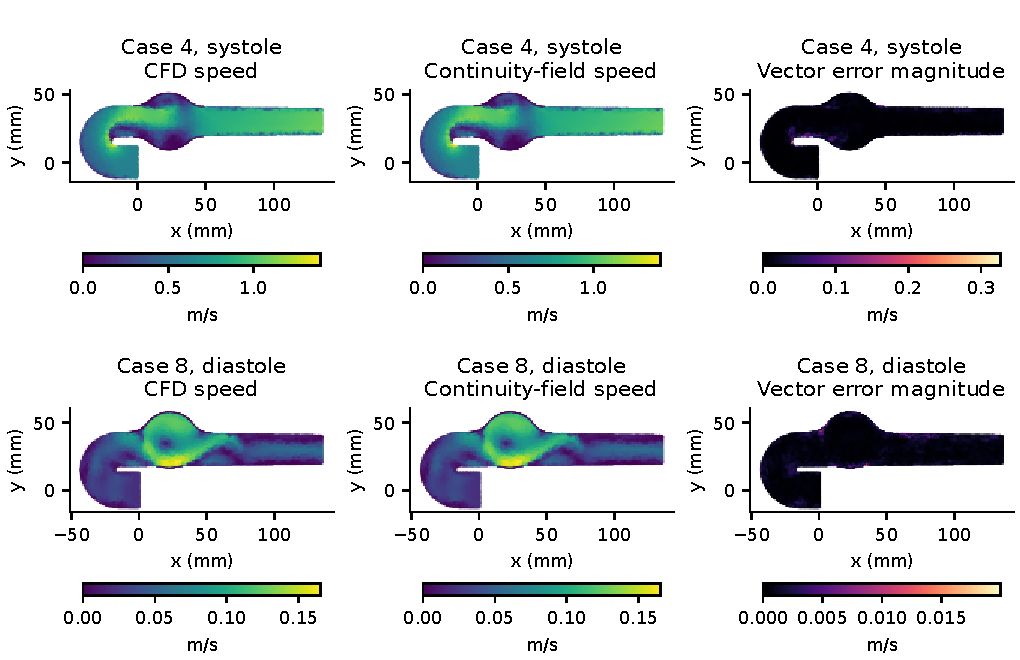
\includegraphics[width=0.90\textwidth]{hidden_velocity_examples.pdf}
\caption{Hidden-node speed on the mid-plane ($|z-z_{\rm mid}|<0.35$~mm) for Case~4 at systole and Case~8 at diastole (draw 0, 2.5~mm). Left, \CFD; center, continuity field; right, magnitude of the vector error. Only unobserved nodes are shown.}
\label{fig:velocity_maps}
\end{figure}

The 99th percentile of aneurysm-zone \WSS is recovered to 0.92 of the \CFD value at systole and 0.90 at diastole, whereas \RBF recovers only 0.52 and 0.61 of it, so \RBF's \WSS error consists mostly of flattened peaks. The Pearson correlation between reconstructed and \CFD \WSS magnitude is 0.92 at systole and 0.94 at diastole for the continuity field, against 0.87 and 0.79 for \RBF, and the \WSS vector errors are 0.38 and 0.20 against 0.62 and 0.42. The systolic pressure drop, which ranges from 413 to 1063~Pa across the cases, is recovered with a median absolute error of 6~Pa against 31~Pa for \RBF. At diastole the median drop errors of 0.48 and 0.67~Pa are comparable to the drops themselves (0.4--5.8~Pa), so neither method recovers the diastolic drop reliably, even though the relative error over the whole pressure field is modest.

The two kinds of error also differ in form. In the median systolic unit (Figure~\ref{fig:field_maps}) the continuity field reproduces the \WSS rings at both necks, while \RBF smears them and underestimates their peaks.

\begin{figure}[H]
\centering
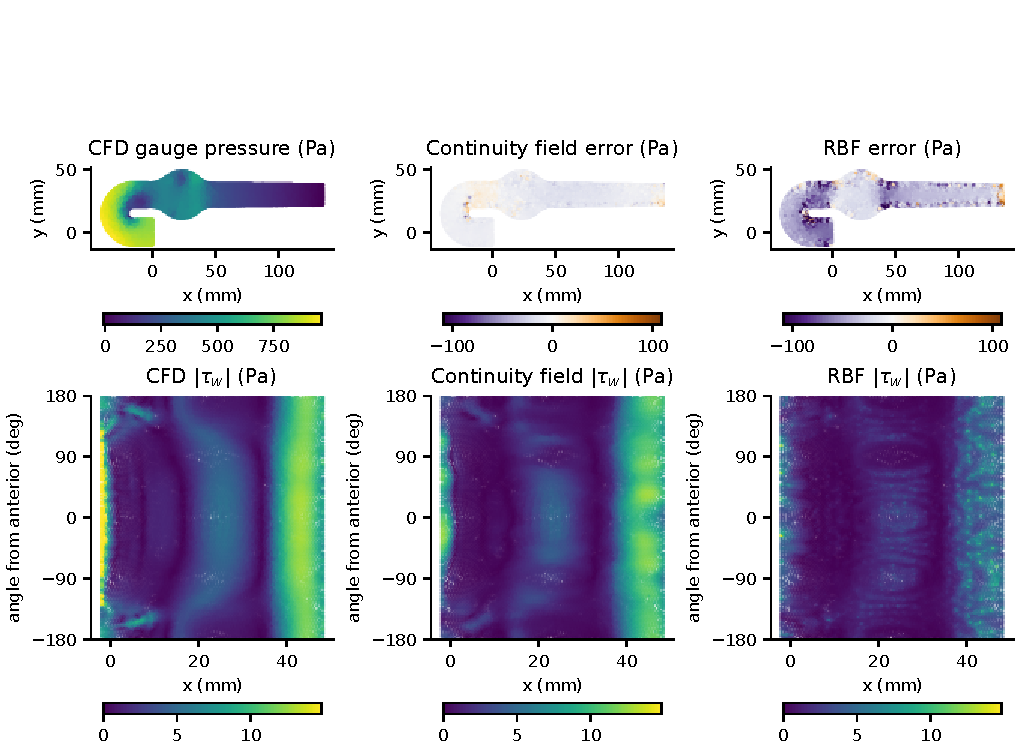
\includegraphics[width=0.95\textwidth]{field_maps_c04_t1780.pdf}
\caption{Case~4 at systole (draw 0, 2.5~mm), close to the median result. Top, \CFD mid-plane pressure and the pressure errors of the continuity field and \RBF. Bottom, aneurysm-zone \WSS unwrapped about the vessel axis. Relative errors are 0.024 and 0.100 for pressure and 0.32 and 0.60 for \WSS.}
\label{fig:field_maps}
\end{figure}

In the adverse diastolic unit (Figure~\ref{fig:field_maps_adverse}), the continuity field's pressure error is a smooth offset of about 1~Pa that accumulates along the vessel, which points to a small bias in the integrated pressure gradient such as the two-snapshot acceleration, while \RBF's pressure errors are concentrated near the sac necks.

\begin{figure}[H]
\centering
\IfFileExists{figures/generated/field_maps_c07_t2400.pdf}{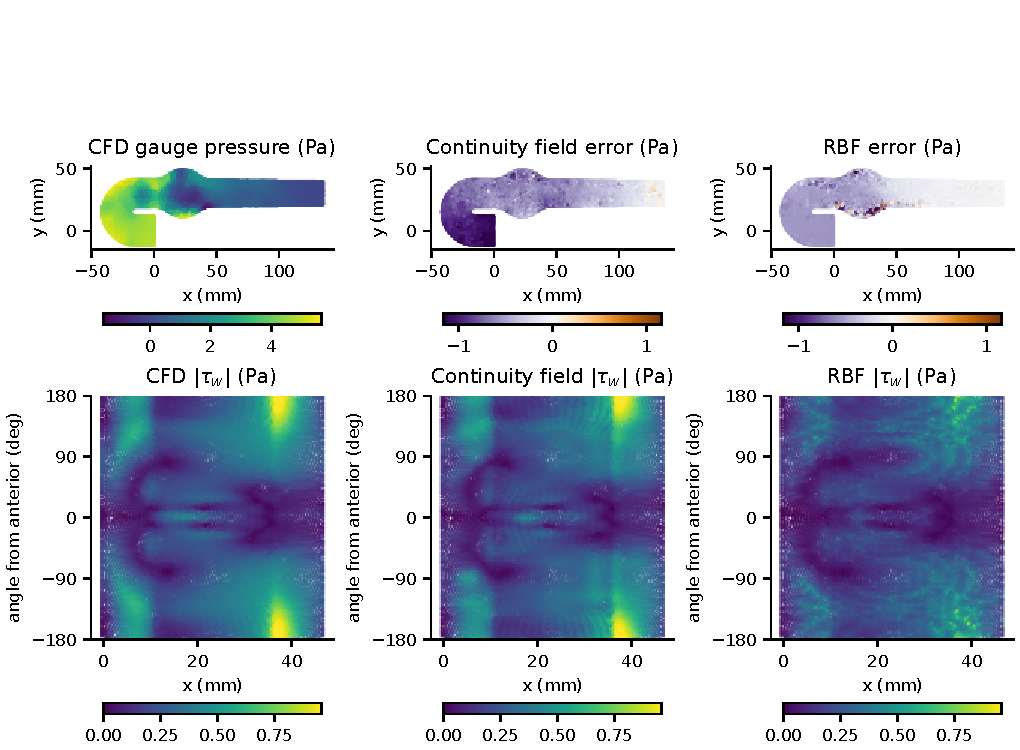
\includegraphics[width=0.95\textwidth]{field_maps_c07_t2400.pdf}}{\fbox{Case 7 diastolic maps pending}}
\caption{As Figure~\ref{fig:field_maps}, for the adverse unit Case~7 at diastole. Relative errors are 0.25 and 0.18 for pressure and 0.14 and 0.33 for \WSS. The \CFD pressure varies by only a few pascals, so errors of about 1~Pa dominate.}
\label{fig:field_maps_adverse}
\end{figure}

The \WSS calculated by automatic differentiation of the continuity field itself was worse than the finite-distance estimate from the same field (median 0.55 against 0.36 in systole and 0.27 against 0.16 in diastole). The soft no-slip penalty fixes the velocity at the wall but leaves its wall-normal gradient poorly determined, so the network's analytic derivative should not be read as \WSS. The finite-distance estimate is also sensitive to $h$. Evaluated at 0.1~mm instead of 0.25~mm, the continuity field's median systolic \WSS error falls from 0.356 to 0.326, and at 0.5~mm it rises to 0.476. We keep the prespecified distance because choosing $h$ with knowledge of the \WSS target would be information that a deployment does not have.

\subsection{Contribution of the continuity penalty and sampling density}
\label{sec:ablation}
Figure~\ref{fig:budget} separates the effect of the continuity penalty from that of the neural representation. At 2.5~mm, the data field without an interior PDE penalty is close to the continuity field, with median velocity errors of 0.052 and 0.039 versus 0.044 and 0.038, and is slightly better on two endpoints, diastolic pressure (0.063 versus 0.094) and systolic \WSS (0.333 versus 0.356). At the densest spacing of 1.5~mm the data field is better on every endpoint except systolic pressure. Only at the sparsest spacing of 4.0~mm, where the observations cover 0.34--0.37\% of the nodes, does the continuity penalty help consistently, reducing the median hidden-velocity error from 0.125 to 0.077 at systole and from 0.105 to 0.077 at diastole, the systolic pressure error from 0.072 to 0.052 and the diastolic \WSS error from 0.371 to 0.316. The main advantage over \RBF therefore comes from fitting one smooth space-time representation to both snapshots, and continuity becomes useful when the data alone no longer determine the field.

The advantage of both neural fields over \RBF grows as the observations become sparser. The median systolic pressure errors at 1.5, 2.5 and 4.0~mm are 0.024, 0.023 and 0.052 for the continuity field versus 0.029, 0.079 and 0.178 for \RBF, and the median systolic \WSS errors are 0.30, 0.36 and 0.48 versus 0.49, 0.61 and 0.68. At diastole and 4.0~mm the continuity field's pressure error is 0.096 versus 0.318 for \RBF. Only one draw was performed at 1.5 and 4.0~mm, so these values describe a trend rather than an uncertainty interval.

\begin{figure}[H]
\centering
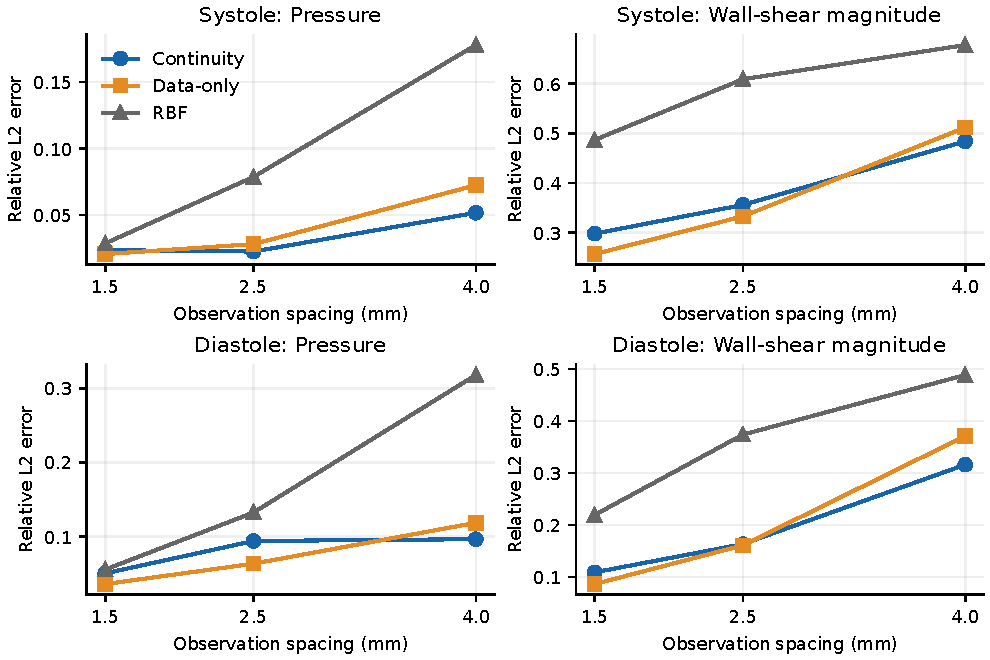
\includegraphics[width=0.92\textwidth]{observation_budget.pdf}
\caption{Median pressure (unsteady form with oracle $\mu_t$) and aneurysm-zone \WSS errors over Cases~2--8 against observation spacing. The 2.5~mm values average three draws per case; 1.5 and 4.0~mm use one draw.}
\label{fig:budget}
\end{figure}

Figure~\ref{fig:pressure_information} asks two separate questions about pressure recovery, namely whether to retain the local acceleration term and whether to supply the \CFD eddy viscosity. Here, steady and unsteady refer to the pressure calculation applied after reconstruction, not to separately trained neural fields. In the seven confirmation geometries, the systolic median improves when the time term is retained and changes little when the eddy viscosity is removed. The unsteady form gives a median error of 0.023 against 0.034 for the steady form, close to the floors of 0.019 and 0.036, and dropping $\mu_t$ changes 0.023 to 0.027. At diastole the eddy viscosity is essential, since removing it more than doubles the continuity field's error, from 0.094 to 0.207, and raises the floor from 0.037 to 0.154. The time term behaves differently for the reconstruction and for the complete \CFD field at diastole. The floor favors the unsteady form (0.037 against 0.065), but the continuity field does better with the steady form (0.072 against 0.094), because the 10~ms finite difference of two reconstructed diastolic fields, whose speeds are about one tenth of the systolic ones, amplifies small reconstruction errors. Diastolic pressure recovery in this setting therefore needs both an estimate of the eddy viscosity and a more accurate acceleration than two sparse snapshots provide.

\begin{figure}[H]
\centering
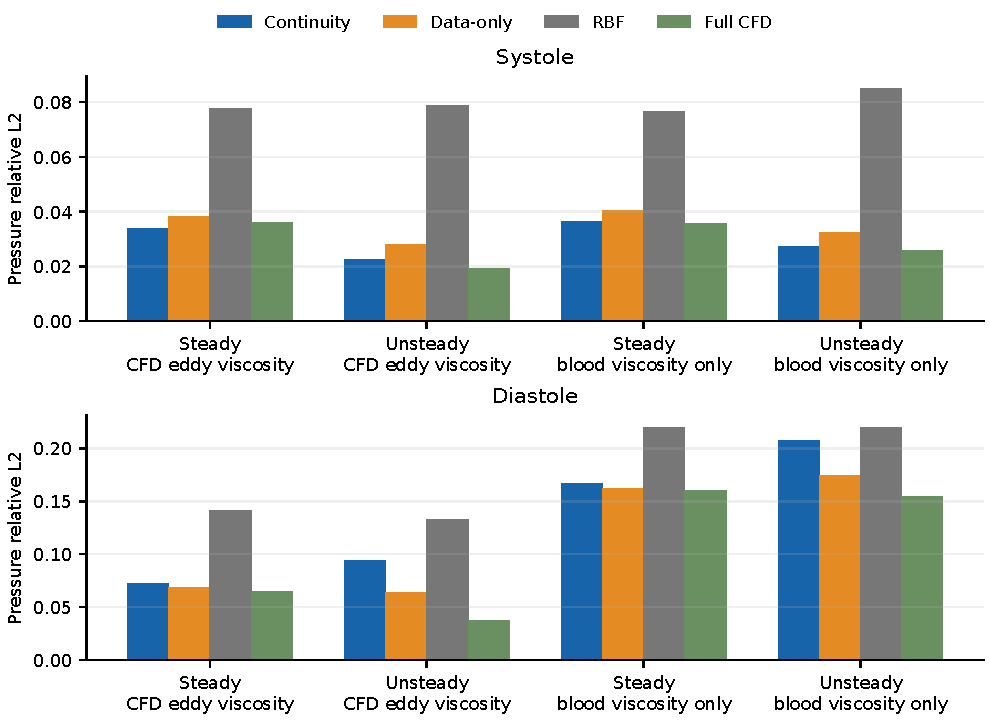
\includegraphics[width=\textwidth]{pressure_information.pdf}
\caption{Median pressure error over Cases~2--8 at 2.5~mm for the four post-processing settings. Unsteady retains the two-snapshot time derivative and steady omits it. ``\CFD eddy viscosity'' uses $\mu+\mu_t$ from the reference simulation, and ``blood viscosity only'' sets $\mu_t=0$. Full \CFD applies the same settings to the complete velocity.}
\label{fig:pressure_information}
\end{figure}

\subsection{Robustness to the choice of interpolation comparator}
\label{sec:robustness}
The prespecified \RBF used one fixed local interpolant in each snapshot. To test how much the comparison depended on that choice, we also evaluated a tuned spatial \RBF and a space-time \RBF, with their settings chosen from the withheld velocity observations. Table~\ref{tab:robustness} reports the completed comparisons for draw 0 at 2.5~mm; these values use one draw per case, so they should be compared within this table rather than directly with the three-draw means of the primary analysis.

At systole, fitting both snapshots with a space-time \RBF changed the median pressure error only slightly, from 0.079 for the prespecified \RBF to 0.074, and the \WSS error from 0.606 to 0.595. The continuity field gave errors of 0.025 and 0.356, respectively, and had lower velocity, pressure and \WSS errors than each \RBF variant in all seven cases. Tuning the spatial \RBF did not improve this phase, since its median pressure and \WSS errors were 0.127 and 0.686; therefore, choosing an interpolant by its velocity error in withheld observations did not ensure lower errors in hidden fields derived from its spatial gradients.

At diastole, both alternatives helped the interpolation. Relative to the prespecified \RBF, the tuned spatial \RBF reduced the median velocity error from 0.129 to 0.100, the pressure error from 0.136 to 0.111 and the \WSS error from 0.371 to 0.321, and the space-time \RBF reduced them to 0.096, 0.113 and 0.301. The continuity field kept lower velocity and \WSS errors than both variants in all seven cases, with a median pressure error of 0.076, but its pressure advantage held in only five of the seven diastolic cases against each variant. Over all 14 case--phase units, the continuity field had the lower pressure error in 12 against the tuned \RBF and in 12 against the space-time \RBF, with median error ratios of 0.50 and 0.54, and the lower \WSS error in all 14 against both, with median ratios of 0.54 and 0.58. It also had a lower pressure error than the better of the two variants in 12 of the 14 units. The comparison against the prespecified \RBF is therefore not an artifact of a weak interpolant, although a stronger interpolant narrows the diastolic pressure gap.

% Generated by generate_robustness_table.py.
\begin{table}[htbp]
\centering
\small
\caption{\revision{\textcolor{red}{Robustness to the interpolation comparator, given as median relative errors over the seven cases in each phase (Cases~2--8) with draw 0 at 2.5~mm. The tuned RBF chooses kernel, neighbourhood and smoothing on the withheld observations, while the space-time RBF interpolates both snapshots jointly with a time scale chosen the same way. All methods share the post-processing, and pressure uses the unsteady form with oracle $\mu_t$.}}}
\label{tab:robustness}
\begin{tabular}{llccc}
\toprule
Phase & Method & Velocity & Pressure & WSS \\
\midrule
Systole & Continuity field & 0.043 & 0.025 & 0.356 \\
Systole & RBF (prespecified) & 0.144 & 0.079 & 0.606 \\
Systole & RBF (tuned) & 0.177 & 0.127 & 0.686 \\
Systole & RBF (space-time) & 0.147 & 0.074 & 0.595 \\
Diastole & Continuity field & 0.038 & 0.076 & 0.173 \\
Diastole & RBF (prespecified) & 0.129 & 0.136 & 0.371 \\
Diastole & RBF (tuned) & 0.100 & 0.111 & 0.321 \\
Diastole & RBF (space-time) & 0.096 & 0.113 & 0.301 \\
\bottomrule
\end{tabular}
\end{table}



\subsection{Sensitivity to near-wall observations}
\label{sec:nearwall}
Because the grid observations are snapped to mesh nodes, some lie on the near-wall prism layers (Section~\ref{sec:observations}). To measure how much the results depend on them, we repeated draw 0 at 2.5~mm for the continuity field and \RBF after removing every observation closer than $\Delta/2=1.25$~mm to the wall, which removed 28--32\% of the observations in each case (Table~\ref{tab:nearwall}). Nothing else was changed.

The \WSS errors rose sharply. For the continuity field the median rose from 0.356 to 0.806 at systole and from 0.173 to 0.521 at diastole, and for \RBF from 0.606 to 0.886 and from 0.371 to 0.681. The accuracy of the one-sided \WSS estimate therefore rests largely on velocity sampled within about a millimetre of the wall, which a 2.5~mm imaging voxel would not resolve. Pressure was much less sensitive. The continuity field's median pressure error changed from 0.025 to 0.027 at systole and from 0.076 to 0.045 at diastole, consistent with pressure being integrated only on nodes more than 1~mm from the wall. The continuity field still had lower velocity, pressure and \WSS errors than \RBF in all 14 units, so the comparison between the methods does not depend on the near-wall samples, whereas the absolute \WSS accuracy does.

% Generated by scripts/manuscript/generate_nearwall_table.py.
\begin{table}[htbp]
\centering
\small
\caption{Sensitivity to near-wall observations. Median relative errors over Cases~2--8 for draw 0 at $\Delta=2.5$~mm, with all observations and with the observations closer than $\Delta/2=1.25$~mm to the wall removed (28--32\% of them). Pressure uses the unsteady form with CFD eddy viscosity; WSS uses $h=0.25$~mm. Velocity is scored on all unobserved nodes, so the second pair of rows is also scored on the removed nodes.}
\label{tab:nearwall}
\begin{tabular}{llccc}
\toprule
Phase & Method and observations & Velocity & Pressure & WSS \\
\midrule
Systole & Continuity field, all observations & 0.043 & 0.025 & 0.356 \\
Systole & RBF, all observations & 0.144 & 0.079 & 0.606 \\
Systole & Continuity field, none within 1.25~mm & 0.130 & 0.027 & 0.806 \\
Systole & RBF, none within 1.25~mm & 0.248 & 0.121 & 0.886 \\
\addlinespace
Diastole & Continuity field, all observations & 0.038 & 0.076 & 0.173 \\
Diastole & RBF, all observations & 0.129 & 0.136 & 0.371 \\
Diastole & Continuity field, none within 1.25~mm & 0.123 & 0.045 & 0.521 \\
Diastole & RBF, none within 1.25~mm & 0.258 & 0.108 & 0.681 \\
\bottomrule
\end{tabular}
\end{table}



\section{Discussion}
\label{sec:discussion}
\subsection{Effects of inlet diameter and asymmetry}
With the flow waveform and the maximum sac diameter held fixed, inlet diameter set the strength of the systolic disturbance and asymmetry set its location. A narrower parent vessel raised the peak Reynolds number, the jet speed entering the sac, the pressure drop, the fraction of reversed flow and the modeled eddy viscosity, and it strengthened the high-shear rings at the necks. This agrees with reports that a larger parent vessel lowers \WSS in intracranial aneurysms~\cite{fattahi2023influence}, and it extends the comparison to transitional flow in a curved, tapered thoracic segment. Because the same flow rate was prescribed for all diameters, the diameter effect here combines the change in geometry with the change in mean velocity. A study that scaled the flow rate with the vessel area would separate these two influences.

Asymmetry moved the low-shear region and the dominant vortex to the side of the larger bulge and shifted the distal high-shear region toward it, while changing the systolic pressure drop by less than 7\%. At diastole its effect became larger than that of diameter, with the asymmetric sacs carrying about two to three times the \WSS of the axisymmetric ones. A previous study of idealized abdominal and descending thoracic aneurysms also found that asymmetry mainly redistributes recirculation and \WSS~\cite{rehman2024comparative}. The present results add that the redistribution depends on the phase of the cycle, so single-instant comparisons at peak systole understate it. None of these comparisons is a population statistic, since each geometry is a single designed case, and whether low or high \WSS relates to growth or rupture cannot be settled by simulations of this kind~\cite{geers2017wall,lipp2020computational}.

\subsection{Why the neural field outperformed interpolation}
The clearest gain came from the reconstructed velocity rather than from adding momentum to the training loss. The neural fields and the prespecified \RBF received the same velocity observations and boundary values, and their pressure and \WSS were computed by the same post-processing. Yet the data field, which has no interior PDE penalty, performed close to the continuity field at 1.5 and 2.5~mm. Both neural fields also retained near-wall gradients that the prespecified \RBF tended to smooth out, and their finite-distance shear estimates recovered about 90--100\% of the \CFD 99th-percentile \WSS, compared with about half for \RBF at systole. The continuity penalty became consistently useful at the sparsest spacing, 4.0~mm.

The network fits one function across the domain and both snapshots, whereas the prespecified \RBF uses a local neighborhood at each time. This difference offers a plausible explanation for the results, but the study does not isolate the effects of spatial smoothness, joint temporal fitting and the network architecture. The space-time \RBF check narrows that interpretation, because fitting both snapshots jointly did not close the gap to the neural field at systole. At diastole, both tuning and joint temporal fitting improved all three median errors of the interpolant and reduced the continuity field's pressure advantage to five of seven cases for draw 0. These checks support the use of a neural representation in this setting without establishing that it is preferable to every interpolation scheme. Related work has used implicit neural representations for 4D flow reconstruction without a physics loss~\cite{saitta2024implicit}; here, the representation supplies velocity to the established momentum-integration route for relative pressure~\cite{krittian2012finite,bertoglio2018relative}.

The momentum \PINNs did not meet the criterion of the development test. Their poor pressure outputs, despite small momentum residuals, are consistent with a weakly determined trade-off between pressure and local acceleration. Two velocity snapshots constrain a finite difference, but they do not uniquely determine the network's time derivative between them. The diagnostic in Section~\ref{sec:pilot_results} showed that a small residual could coexist with an inaccurate pressure field. This fits the broader sensitivity of \PINNs to loss weighting and the information available to each residual~\cite{krishnapriyan2021failure,wang2021gradient}. Recovering pressure after fitting avoids relying on that pressure head, although the two-snapshot acceleration still carries reconstruction error. Longer time series, hard constraints and other loss weights might change the comparison. They were not tested here, so the negative result applies to the specified formulation and windows rather than to momentum \PINNs in general~\cite{mcgreivy2024weak}.

\subsection{Information needed for each hidden field}
Pressure and \WSS expose different weaknesses in the reconstruction of the sparse velocity. For the seven confirmation geometries, the retention of local acceleration brought the median systolic pressure error close to the complete-\CFD post-processing reference. Removing eddy viscosity did little to change that median, although the reference study of all-cases showed greater sensitivity in narrower geometries of 2.0~cm. The limited systolic sensitivity of the median should therefore not be read as evidence that eddy viscosity can always be neglected.

At diastole, omitting the \CFD eddy viscosity raised even the complete-velocity pressure error to 9--19\%. The reconstruction results with that field supplied describe a conditional calculation, because the sparse velocity observations do not themselves provide the closure. Small absolute pressure errors also matter more in this phase. None of the tested methods reliably recovered the diastolic pressure drop, even when its relative error across the field appeared modest. An estimate of eddy viscosity and a better-resolved acceleration are, therefore, separate requirements to examine before applying this calculation to measured data.

For aneurysm-zone \WSS, near-wall sampling remained the main limitation. Removing the observations within 1.25~mm of the wall more than doubled the continuity field's \WSS error at both phases while leaving the ranking against \RBF unchanged (Section~\ref{sec:nearwall}). The error depended on the distance used by the one-sided estimate, and the reconstructed fields remained above the complete-\CFD reference. Outside the aneurysm zone, the interior node closest to the wall was a median of 0.58~mm from it; even the complete \CFD velocity then gave a poor estimate of the exported shear. This is consistent with the documented sensitivity of velocity-derived \WSS to spatial resolution~\cite{petersson2012assessment,stalder2008quantitative}. A smooth velocity fit and an analytic derivative do not, by themselves, establish an accurate wall gradient.

\subsection{Limitations}
\label{Limitations}
The twelve geometries form a designed family, not a patient cohort. They share one maximum aneurysm diameter, taper ratio and inflow waveform, and they contain no branches. The seven confirmation geometries therefore test variation within that family. The rigid-wall flow solution has reported mesh, time-step and cycle checks for aneurysm \WSS, but no experimental validation. The structural calculation uses a uniform 2~mm wall, literature material parameters, fixed ends and a quasi-static coupling. Its coupling-step and mesh-update settings were not retained with the results, and no solid-mesh convergence check is available, so the stress fields are used only to describe modeled stress concentrations.

The temporal records also have limits. Each reconstruction uses two snapshots from a short window. Several instants were retained, but no complete cycle-resolved wall-traction series is available. The solver exported \TAWSS to the wall nodes, but its cycle-resolved components did not, so the oscillatory indices were not evaluated. The slice workbook does not state its averaging interval; the slice values were identified as cycle averages from the inlet flow rate.

The observed velocities are noise-free \CFD values at the mesh nodes. They do not include partial-volume averaging, noise, segmentation error, or velocity aliasing of 4D flow MRI~\cite{markl2012fourd}, and some lie within a fraction of a millimeter of the wall (Section~\ref{sec:observations}). Without observations within 1.25~mm of the wall, the \WSS errors were more than twice as large (Section~\ref{sec:nearwall}), so the absolute \WSS precision reported here should not be expected from the imaging data. Performance on measured data may therefore be worse. Pressure calculations with \CFD-supplied eddy viscosity additionally assume closure information that would have to be estimated in practice. The errors are node-weighted because the exports contain no cell volumes, which gives a greater weight to the refined near-wall mesh.

The network architecture and training settings were fixed on the development cases without a wider hyperparameter search. The tuned and space-time \RBF checks were added after the primary verdict and use one draw per case; they cannot replace the three-draw comparison. A divergence-free interpolant, the natural non-neural counterpart of the continuity field, was not tested. Every method receives observations in the target geometry. The prediction in a geometry with no observations was not tested. Finally, fitting a neural field took about 20~min on a GPU per window, so its accuracy came at a higher computational cost than interpolation.

\section{Conclusion}
\label{sec:conclusion}
Twelve idealized descending thoracic aortic geometries with a fixed maximum sac diameter of 4.0~cm were simulated with transient transitional \CFD, and their common-time fields were used both to compare the geometries and to test the recovery of hidden pressure and \WSS from sparse velocity. The inlet diameter dominated the systolic response. Reducing it from 2.6 to 2.0~cm raised the pressure drop 2.3--2.5 times, roughly doubled the fraction of reversed flow in dilation, and raised the 95th-percentile \WSS in the necks from 7--8 to 15--18~Pa, while the bulge pattern changed the drop in systolic pressure by less than 7\%. Instead, asymmetry relocated the low-shear region and the dominant vortex to the larger bulge, and at diastole it raised the median \WSS of the dilation segment 1.8--3.1 times relative to the axisymmetric sacs.

With velocity observed at about 1.3\% of the interior nodes at two instants, a continuity-constrained space-time neural field followed by momentum integration and a near-wall shear estimate recovered pressure and aneurysm-zone \WSS more accurately than the same post-processing applied to the prespecified \RBF in all 14 confirmation units after averaging three draws per unit, with median error ratios of 0.46 and 0.51. The pressure advantage was small at diastole. The benefit came mainly from the neural representation of the velocity. A continuity penalty helped in the sparsest sampling, and momentum \PINNs did not meet the development-test criterion for joint pressure and shear recovery. Systolic pressure was recovered close to the accuracy of post-processing itself, diastolic pressure required the \CFD eddy viscosity as an input to the oracle, and \WSS accuracy depended on the velocity sampled close to the wall, although the continuity field retained its advantage over \RBF without those samples. These findings identify what information each hidden field needs in this idealized, noise-free setting. Measured velocity data, estimated closures, and patient-specific anatomies are the next tests, and none of the results constitutes a clinical rupture-risk assessment.

\section*{Declarations}
\paragraph{Conflicts of interest.} The authors have no conflicts to disclose.

\ifanonymized
\paragraph{Funding and author contributions.} Removed for anonymized review.
\else
\paragraph{Funding.} Helmi Temimi thanks the Kuwait Foundation for the Advancement of Sciences (Project Code: CN22-16QE-1643).

\paragraph{Author contributions.} Conceptualization, M.A.U.R. and M.A.O.; \CFD and structural modeling, M.A.U.R.; reconstruction methodology, software and formal analysis of the reconstruction study, M.A.O.; validation, M.A.U.R., M.A.O., F.J. and H.T.; data curation, M.A.U.R. and M.A.O.; writing (original draft), M.A.U.R. and M.A.O.; writing (review and editing), all authors; funding acquisition, F.J. and H.T. All authors have read and agreed to the submitted version.
\fi


% \paragraph{Use of generative AI.} During the preparation of this work, the authors used Claude (Anthropic) and Codex (OpenAI) to help write and edit the language and grammar of the manuscript. The simulations, the study design and the interpretation of the results are the authors' own. The authors reviewed and edited all AI-assisted output and take full responsibility for the content of the publication.

\paragraph{Data availability statement.} The \CFD exports analyzed in this study are available from the corresponding author on reasonable request. \ifanonymized The reconstruction code and configuration files are available in a public repository whose link is withheld for anonymized review.\else The reconstruction code and configuration files are available at \url{https://github.com/michaelajao/IdealAorta-PINN}.\fi

\appendix
\section{Case-wise reconstruction results}
\label{app:casewise}
Tables~\ref{tab:case_pressure} and \ref{tab:case_shear} list every confirmation unit at 2.5~mm, spread over the three paired draws and the range of draw-wise error ratios to \RBF.

\begin{table}[htbp]
\centering
\small
\caption{Case-wise pressure relative L2 at 2.5~mm, given as the mean (sample standard deviation) over three paired observation/initialization draws. The last column is the range of draw-wise continuity/RBF error ratios, and values above one favor RBF. The spread describes these draws, not patient-population uncertainty.}
\label{tab:case_pressure}
\begin{tabular}{llcccc}
\toprule
Case & Phase & Continuity & Data-only & RBF & Ratio range \\
\midrule
2 & Sys. & 0.069 (0.004) & 0.069 (0.008) & 0.111 (0.010) & 0.53--0.68 \\
2 & Dia. & 0.094 (0.026) & 0.050 (0.012) & 0.138 (0.016) & 0.55--0.81 \\
3 & Sys. & 0.031 (0.004) & 0.030 (0.004) & 0.078 (0.009) & 0.35--0.47 \\
3 & Dia. & 0.028 (0.004) & 0.032 (0.003) & 0.095 (0.014) & 0.27--0.32 \\
4 & Sys. & 0.023 (0.001) & 0.027 (0.008) & 0.093 (0.019) & 0.20--0.30 \\
4 & Dia. & 0.107 (0.032) & 0.071 (0.020) & 0.157 (0.018) & 0.50--1.05 \\
5 & Sys. & 0.022 (0.002) & 0.028 (0.002) & 0.079 (0.011) & 0.24--0.31 \\
5 & Dia. & 0.044 (0.017) & 0.059 (0.027) & 0.113 (0.015) & 0.29--0.56 \\
6 & Sys. & 0.020 (0.000) & 0.027 (0.004) & 0.081 (0.017) & 0.20--0.30 \\
6 & Dia. & 0.085 (0.029) & 0.093 (0.031) & 0.132 (0.004) & 0.51--0.89 \\
7 & Sys. & 0.021 (0.004) & 0.022 (0.003) & 0.074 (0.015) & 0.25--0.34 \\
7 & Dia. & 0.155 (0.085) & 0.090 (0.035) & 0.171 (0.008) & 0.54--1.40 \\
8 & Sys. & 0.032 (0.005) & 0.030 (0.009) & 0.063 (0.007) & 0.50--0.54 \\
8 & Dia. & 0.101 (0.076) & 0.063 (0.011) & 0.104 (0.005) & 0.31--1.75 \\
\bottomrule
\end{tabular}
\end{table}

\begin{table}[htbp]
\centering
\small
\caption{Case-wise wall-shear magnitude relative L2 at 2.5~mm, given as the mean (sample standard deviation) over three paired observation/initialization draws. The last column is the range of draw-wise continuity/RBF error ratios, and values above one favor RBF. The spread describes these draws, not patient-population uncertainty.}
\label{tab:case_shear}
\begin{tabular}{llcccc}
\toprule
Case & Phase & Continuity & Data-only & RBF & Ratio range \\
\midrule
2 & Sys. & 0.417 (0.007) & 0.386 (0.018) & 0.653 (0.004) & 0.63--0.65 \\
2 & Dia. & 0.166 (0.009) & 0.169 (0.029) & 0.404 (0.002) & 0.39--0.43 \\
3 & Sys. & 0.363 (0.010) & 0.333 (0.026) & 0.636 (0.008) & 0.55--0.60 \\
3 & Dia. & 0.166 (0.006) & 0.148 (0.013) & 0.409 (0.005) & 0.39--0.43 \\
4 & Sys. & 0.329 (0.033) & 0.306 (0.018) & 0.605 (0.001) & 0.51--0.61 \\
4 & Dia. & 0.131 (0.004) & 0.150 (0.020) & 0.302 (0.002) & 0.42--0.44 \\
5 & Sys. & 0.356 (0.005) & 0.359 (0.011) & 0.619 (0.010) & 0.56--0.59 \\
5 & Dia. & 0.163 (0.018) & 0.174 (0.008) & 0.386 (0.001) & 0.37--0.45 \\
6 & Sys. & 0.373 (0.002) & 0.352 (0.027) & 0.609 (0.005) & 0.61--0.62 \\
6 & Dia. & 0.155 (0.030) & 0.161 (0.008) & 0.368 (0.003) & 0.33--0.50 \\
7 & Sys. & 0.323 (0.012) & 0.300 (0.011) & 0.590 (0.005) & 0.53--0.57 \\
7 & Dia. & 0.136 (0.004) & 0.146 (0.019) & 0.332 (0.005) & 0.40--0.43 \\
8 & Sys. & 0.330 (0.012) & 0.327 (0.009) & 0.598 (0.005) & 0.54--0.58 \\
8 & Dia. & 0.176 (0.022) & 0.196 (0.013) & 0.374 (0.005) & 0.40--0.51 \\
\bottomrule
\end{tabular}
\end{table}


\newpage
\bibliographystyle{unsrt}
\bibliography{bib/tsb,bib/references}

\end{document}
"
\newif\ifanonymized
\ifdefined\anonymized\anonymizedtrue\fi

\begin{document}

\begin{center}

{\Large \bf
% Hemodynamics of Idealized Descending Thoracic Aortic Aneurysms and Physics-Based Recovery of Pressure and Wall Shear Stress from Sparse Velocity

Effects of Inlet Diameter and Sac Asymmetry on Transitional Flow in Idealized Descending Thoracic Aortic Aneurysms, with Neural-Field Recovery of Pressure and Wall Shear Stress from Sparse Velocity
}\\[12mm]

% Continuity-Constrained Space-Time Neural Fields Improve Pressure and Wall Shear Stress Recovery from Sparse Velocity in Idealized Descending Thoracic Aortic Aneurysms

\ifanonymized\else
{\bf
M. Abaid Ur Rehman$^{a,b,*}$,
{Michael Ajao-Olarinoye$^{c}$},
Fei Jia$^{a,**}$,
Helmi Temimi$^{d}$
}\\[3mm]

{$^{a}$Department of Astronautical Science and Mechanics,
Harbin Institute of Technology, Harbin 150001, China}\\

{$^{b}$Department of Mathematics, School of Natural Sciences (SNS),
National University of Sciences and Technology (NUST),
Sector H-12, 44000, Islamabad, Pakistan}\\

{
$^{c}$Computational Science and Mathematical Modelling (CSMM),
Coventry University, Coventry, United Kingdom
}\\

{$^{d}$College of Integrative Studies,
Abdullah Al Salem University, Khaldiya, Kuwait}\\[3mm]
\fi

\end{center}

\ifanonymized\else
\noindent
$^{*}$\textbf{Corresponding author:}
M. Abaid Ur Rehman,
Email:
\href{mailto:abaidurrehman803@gmail.com}
{abaidurrehman803@gmail.com}

\vspace{1mm}

\noindent
$^{**}$\textbf{Corresponding author:}
Fei Jia,
Email:
\href{mailto:jiafei0009@163.com}
{jiafei0009@163.com}

\vspace{3mm}

\begin{center}
\textbf{Emails:}
\href{mailto:abaidurrehman803@gmail.com}
{abaidurrehman803@gmail.com},
{
\href{mailto:ajaoolarinoyemichael@gmail.com}
{ajaoolarinoyemichael@gmail.com}},
\href{mailto:jiafei0009@163.com}
{jiafei0009@163.com},
\href{mailto:helmi.temimi@aasu.edu.kw}
{helmi.temimi@aasu.edu.kw}
\end{center}
\fi

\begin{abstract}
Twelve idealized \DTAA models were constructed using three inlet diameters (\num{2.0}, \num{2.3}, and \SI{2.6}{\centi\metre}). For each inlet diameter, one axisymmetric aneurysm, two asymmetric aneurysms (anterior-dominant and posterior-dominant), and one healthy control model were considered. The maximum aneurysm diameter was fixed at \SI{4}{\centi\metre} for all aneurysmal cases, with a fixed vessel taper ratio of 0.8 from inlet to outlet. Narrowing the inlet from 2.6 to 2.0~cm increased the pressure drop from 528--561 to 1261--1346~Pa, the reverse flow fraction in dilation from 24--28\% to 50--54\%, and the 95th-percentile \WSS from 7--8 to 15--18~Pa, while the bulge pattern changed the pressure drop by at most 7\%. Instead, asymmetry relocated low \WSS to the dominant bulge and, at diastole, raised the median \WSS of the dilation segment 1.8--3.1 times above that of the axisymmetric sacs. The recovery of hidden pressure and aneurysm-zone \WSS was tested from the velocity observed at about 1.3\% of the interior nodes at two instants 5--10~ms apart. Linear and \RBF interpolation and space-time neural fields, with and without a continuity penalty, were passed through identical momentum-integration and near-wall shear calculations. Under a protocol fixed on two development geometries, the continuity-constrained field reduced pressure and \WSS errors relative to \RBF in all 14 case phase units of seven geometries not used for tuning, with median error ratios of 0.46 and 0.51, and a systolic pressure error (2.3\%) close to that from the complete \CFD velocity (1.9\%). The diastolic pressure advantage was small. The gain was mainly due to the neural representation. In two development geometries, \PINNs penalizing the residual momentum recovered pressure far less accurately than integration after fitting. Diastolic pressure required the \CFD eddy viscosity as an oracle, and \WSS accuracy required velocity sampled within about a millimeter of the wall. The results define the information each hidden field requires in idealized and noise-free conditions and are not a clinical rupture-risk assessment.
\end{abstract}
\acresetall

\noindent\textbf{Keywords.} Thoracic aortic aneurysm; computational fluid dynamics; wall shear stress; sparse flow reconstruction; physics-informed neural networks; relative pressure estimation


\section{Introduction}
\label{sec:introduction}

The cardiovascular system circulates blood throughout the body, delivering oxygen and nutrients while removing waste products~\cite{heymans1960reflexogenic}. Arteries consist of three layers~\cite{holzapfel2010modelling}: the tunica intima (innermost, endothelial cells that reduce friction), media (middle, muscular layer regulating constriction and dilation), and externa (outermost, structural support). The aorta, the largest vessel in the body, comprises the ascending aorta, the aortic arch, and the descending thoracic aorta before becoming the abdominal aorta in the diaphragm. The thoracic aorta supplies oxygenated blood to the head, neck, upper extremities, and thoracic structures~\cite{tran2018anatomy}.

Cardiovascular disease is a leading cause of mortality, affecting nearly 92 million adults in the United States and projected to affect 43.9\% of the population by 2030~\cite{Randles_CFD_2017}. Arterial disease includes atherosclerosis, stenosis, thrombus formation, and aneurysms. An aneurysm is an abnormal bulge~\cite{Les_et_al_2010}, classified as saccular (one-sided) or fusiform (circumferential)~\cite{sakalihasan2018abdominal}. Elective repair is often determined by maximum diameter, with various anatomical factors proposed as predictors of severity~\cite{cronenwett1990variables, lipp2020computational}. However, these standards lack precision: aneurysms of the same maximum diameter can vary in shape, wall thickness, and mechanical properties, affecting growth and risk of rupture. A surgery based on a 5~cm criterion may therefore be unjustifiable or delayed inappropriately, since rupture can occur below this threshold~\cite{darling1977autopsy, belkacemi2022flow}. Since rupture occurs when mechanical stress exceeds tissue tensile strength, risk assessment based on \WSS and hemodynamics provides more accurate prediction~\cite{bilgi2020effects, vorp1998mechanical}. Kitagawa et al.~\cite{kitagawa2013role} further suggest that aneurysm volume is more reliable than maximum diameter because it captures the entire 3D shape and detects subtle growth more consistently.

\CFDcap plays an important role in the study of vascular disease progression, particularly blood flow behavior in abnormal arteries~\cite{lee2011computational}. It uses numerical methods to solve the Navier--Stokes equations for flow fields, velocity, and stresses~\cite{navier1823memoire, stokes2007theories}, aiding early diagnosis and risk assessment~\cite{morris2016computational}. Commonly used parameters include \WSS, \WSSG, and \OSI. Both high and low \WSS are associated with aneurysm disease: high \WSS contributes to initiation by weakening the intima, while low \WSS promotes growth and rupture~\cite{geers2017wall}. Moon et al.~\cite{moon2025hemodynamic} studied four ruptured fusiform infrarenal aneurysms and found rupture in regions of low \TAWSS, high \OSI, \RRT, and \ECAP. Kumar et al.~\cite{SK1} reported that saccular aneurysms exhibit complex streamline patterns and low-\WSS regions.

Arterial tortuosity, the bending and twisting of vessels, alters local flow patterns and causes disturbed hemodynamics~\cite{9a}. Inflow conditions, and thus velocity and \WSS distributions, are determined by parent vessel diameter, which feeds the aneurysm. These geometric factors jointly regulate intra-aneurysmal flow, affecting growth, thrombosis, and rupture. Buradi et al.~\cite{10a} analyzed idealized tortuous geometries, varying curvature radius, bending angle, and inter-bend distance, and found that regions with high \RRT, significant \TAWSS gradient, and lower \OSI are more susceptible to plaque development and rupture. Nagargoje et al.~\cite{11a} modeled C-, U-, S-shaped, and helical \ICA bends, concluding that parent artery morphology significantly affects local hemodynamics. Tortuosity effects have also been studied in abdominal~\cite{12a}, descending thoracic~\cite{13a}, and cerebral aneurysms~\cite{14a}. Fattahi et al.~\cite{fattahi2023influence, fattahi2023usage} found that increasing parent-vessel diameter decreases \WSS and \OSI in \ICA sacs. Nagargoje et al.~\cite{nagargoje2022influence} showed that increasing \AR and \SR raises near-neck \WSS, \OSI, and \RRT in patient-specific models.

Laminar flow is typical in a healthy aorta, but aneurysms introduce irregular geometries and pulsatile flow that disturb the streamlines. Transitional or turbulent flow occurs in clinical conditions such as aneurysms and other vascular diseases, and the resulting instabilities and vortex structures require turbulence models for accurate hemodynamic analysis. Brambila-Solórzano et al.~\cite{brambila2023influence} discussed how turbulent modeling affects \WSS and \TAWSS prediction in aneurysms, which is crucial for identifying high-risk rupture regions. Turbulence models such as $k-\epsilon$ or \DNS resolve chaotic flow structures and better estimate pressure drop, flow separation, and vortex formation. Such modeling is vital for capturing complex unstable patterns overlooked by laminar assumptions, particularly in regions with disturbed flow. These disturbances often lead to transitional or turbulent flow even at moderate Reynolds numbers~\cite{evju2015assumption}, particularly within aneurysmal regions. Luciano et al.~\cite{luciano2024turbulent} investigated turbulence in cerebral aneurysms despite low sac Reynolds numbers, noting that neglecting turbulent effects can introduce errors. Rawat et al.~\cite{rawat2019numerical} similarly emphasized that arterial flow can be transitional, with vortices forming after systole. Accurate turbulent flow modeling is therefore essential for capturing hemodynamic parameters such as \WSS and \OSI.

Several studies have investigated aneurysm hemodynamics using patient-based and idealized geometries. Lauric et al.~\cite{lauric2019proximal} examined 33 middle cerebral artery aneurysm patients and 44 controls, finding aneurysmal arteries have a tapered parent vessel (mean ratio 0.88) versus near-unity in healthy vessels; tapering elevates \WSS and \WSSG, promoting aneurysm formation. Jin et al.~\cite{jin2023cfd} reported that reducing coil porosity from 0.89 to 0.79 decreases \OSI by up to 55\% in an \ICA aneurysm. Tian et al.~\cite{tian2023influence} used 18 idealized and 7 patient-specific bifurcation aneurysms to show that the aneurysm--parent vessel angle dominates \LDL deposition, with larger angles promoting deposition by reducing inflow and enhancing stagnation. Rehman et al.~\cite{ur2025fluid} studied Marfan syndrome aneurysms using \FSI with \CFD and \PINNs on six patient-specific models, observing that \WSS disturbances vary with shape and that the anterior wall experiences higher stresses. Zhou et al.~\cite{zhou2026morphological} developed an AutoML model on 158 intracranial aneurysms, identifying bifurcation angle as the most critical risk factor. These patient-based studies, however, are confounded by multiple simultaneously varying anatomical features, making it difficult to isolate single-parameter effects. Idealized geometries offer systematic parameter variation.

Previous idealized studies have largely overlooked physiological tapering (i.e., the progressive reduction in vessel diameter from inlet to outlet), the isolated influence of parent vessel diameter, and the relationship between hemodynamic and morphometric characteristics of the aorta for both axisymmetric (fusiform) and asymmetric (saccular) geometries of \DTAA (Table~\ref{tab:lit_review}). To address these gaps, the present study introduces a set of twelve idealized geometries of the descending thoracic aorta, including nine with aneurysms and three healthy ones without aneurysms. The entire vessel, from inlet to outlet, is modeled with a linear taper characterized by a fixed taper ratio of 0.8 (i.e., outlet diameter $= 0.8 \times$ inlet diameter), consistent with physiological observations. Three different diameters of inlets (2.0~cm, 2.3~cm and 2.6~cm) are used to study the effect of parent vessel size, and a localized aneurysm is simulated with a fixed maximum diameter of 4~cm in the descending thoracic segment. For each inlet diameter, three aneurysm morphologies are examined, namely axisymmetric (fusiform), anterior-dominant asymmetric (saccular), and posterior-dominant asymmetric (saccular), reflecting clinically observed variations. Unlike the ascending aorta, the descending thoracic aorta is characterized by an upstream curvature, significantly affecting the flow dynamics upstream of aneurysm formation. Thus, in this study, the investigation of parent vessel diameter and physiological tapering, aneurysm asymmetry, and flow dynamics in \DTAA is considered.

Resolving each of these geometries with \CFD is computationally demanding, which limits how densely the diameter--asymmetry space can be sampled and how readily the analysis extends to a new vessel size. The same fields also raise a second, methodological question, because the quantity that is measured clinically is velocity, not pressure or \WSS. Time-resolved three-dimensional phase-contrast MRI (4D flow MRI) samples the lumen on voxels of roughly one to three millimeters~\cite{markl2012fourd}, whereas relative pressure and \WSS have to be derived from those samples. Relative pressure can be computed from measured velocity by pressure-Poisson, work--energy and related formulations of the momentum balance~\cite{krittian2012finite, bertoglio2018relative}, and \WSS estimated from phase-contrast velocity depends strongly on spatial resolution and wall segmentation and is usually underestimated~\cite{stalder2008quantitative, petersson2012assessment, potters2015volumetric}. \PINNs and related neural fields offer another route, fitting a continuous representation to sparse velocity while penalizing violations of the governing equations~\cite{raissi2019pinn, raissi2020hfm}. They have been used to infer arterial pressure from 4D flow data~\cite{kissas2020machine}, to super-resolve and denoise 4D flow fields~\cite{fathi2020super, saitta2024implicit}, to recover near-wall flow and \WSS from sparse velocity~\cite{arzani2021nearwall} and to reconstruct aneurysm flow~\cite{cruzgonzalez2025aaa}. \PINN training can fail for reasons unrelated to the available information~\cite{krishnapriyan2021failure, wang2021gradient}, and a survey of machine learning for fluid-related partial differential equations found that most reported advantages were measured against weak baselines~\cite{mcgreivy2024weak}.

Two points are rarely separated in this literature, and both matter in pulsatile transitional flow. The first is how much of any improvement over conventional interpolation comes from the neural representation itself and how much from the physics terms added to its loss. The second is what information beyond sparse velocity the hidden fields actually require, because in unsteady Reynolds-averaged flow the pressure gradient also depends on local acceleration and on the eddy viscosity, neither of which is measured directly. A fair test needs matched observations for every method, one shared route from velocity to pressure and \WSS, and an explicit account of every additional input. Table~\ref{tab:lit_review} compares the present study with earlier idealized aneurysm studies on these points and on the modeling choices discussed above.


\begin{table}[htbp]
\centering
\footnotesize
\caption{Comparison of existing idealized aneurysm studies and the present work, emphasizing differences in geometry, flow modeling, boundary conditions, hemodynamic--morphometric analysis, and sparse-velocity reconstruction.}
\setlength{\tabcolsep}{3pt}
\begin{tabular}{|>{\raggedright\arraybackslash}p{4.0cm}|*{6}{>{\centering\arraybackslash}p{1.78cm}|}}
\hline
\textbf{Feature} & \parbox{1.78cm}{\textbf{Jin et al.~\cite{jin2021arterial}}} & \parbox{1.78cm}{\textbf{Guerrero-Hurtado et al.~\cite{guerrero2023efficient}}} & \parbox{1.78cm}{\textbf{Rehman et al.~\cite{rehman2024comparative}}} & \parbox{1.78cm}{\textbf{Rehman et al.~\cite{rehman2025application}}} & \parbox{1.78cm}{\textbf{Moroni \& Espa~\cite{moroni2025insight}}} & \parbox{1.78cm}{\textbf{Present Study}} \\
\hline
Year & 2021 & 2023 & 2024 & 2025 & 2025 & - \\
\hline
Geometry Type & Idealized & Idealized & Idealized & Idealized & Idealized & Idealized \\
\hline
\DTAA & No & No & Yes & No & No & Yes \\
\hline
{Arterial Tapering} & No & No & No & No & No & Yes \\
\hline
Parent vessel effect & No & No & No & No & No & Yes \\
\hline
\parbox{3.7cm}{Morphology: Axisymmetric or Asymmetric} & Not varied & Not varied & Both & Both & Both & Both \\
\hline
\parbox{3.7cm}{SST $k-\omega$ Transition Turbulence Model} & No & No & No & No & No & Yes \\
\hline
Transient Flow Inlet & Yes & Yes & No & No & No & Yes \\
\hline
\parbox{3cm}{Transient Pressure Outlet} & Yes & No & No & No & No & Yes \\
\hline
Plane-wise flow--morphometry analysis & Partial & No & No & Partial & Partial & Yes \\
\hline
\PINNcap & No & No & Yes & No & No & Tested on two cases \\
\hline
Hidden pressure and \WSS from sparse velocity against matched baselines & No & No & No & No & No & Yes \\
\hline
\end{tabular}%
\label{tab:lit_review}
\end{table}



This study addresses both questions on a family of twelve idealized descending thoracic aortic geometries, namely nine aneurysmal models formed by three inlet diameters and three bulge patterns at a fixed 4.0~cm maximum sac diameter, and three nonaneurysmal controls. The contributions are as follows.
\begin{enumerate}
\item We report how inlet diameter and sac asymmetry change pressure drop, reversed flow, eddy viscosity and aneurysm-zone \WSS in transient transitional \CFD, evaluated at common systolic and diastolic instants for all twelve geometries.
\item We define a sparse-reconstruction task on the same fields, in which velocity is observed at about 1.3\% of the interior nodes at two instants 5--10~ms apart and hidden pressure and aneurysm-zone \WSS must be recovered in the known geometry. Linear interpolation, \RBF interpolation and space-time neural fields with and without a continuity penalty all pass through the same momentum-integration and near-wall shear calculations, so their differences are attributable to the reconstructed velocity alone.
\item Using a protocol fixed on two development geometries before evaluation on seven others, we separate the contributions of the neural representation, the continuity constraint, the local time derivative and the eddy-viscosity closure. On two development geometries, we also report that the pressure output of a \PINN with the momentum residual in its loss was far less accurate than momentum integration applied after fitting.
\end{enumerate}
The two parts belong together because the parametric family supplies reference fields whose jet strength, recirculation and modeled eddy viscosity vary systematically with geometry, so the reconstruction test can show how recovery depends on these flow features rather than on a single case. The reconstruction concerns a known geometry with noise-free velocity sampled from \CFD. It does not test prediction for an unseen anatomy, and it does not establish clinical rupture risk.


\section{\label{Material and Methods}Materials and methods}
\subsection{\label{Geometric Description}Geometric description}
Twelve idealized descending-aortic geometries were examined, namely nine aneurysmal models and three nonaneurysmal (healthy) controls. The aneurysmal group used three inlet diameters, 2.0, 2.3 and 2.6~cm. An axisymmetric and two asymmetric aneurysm shapes were studied for each inlet diameter. The level of asymmetry was calculated as the ratio $\beta = r/R$, where $r$ and $R$ denote the characteristic radii of the aneurysmal segment in the posterior and anterior directions, respectively. An axisymmetric bulge gives $\beta = 1$; {a} posterior-dominant bulge gives $\beta > 1$ and {an} anterior-dominant bulge $\beta < 1$, the two representing opposite directional dilations. The detailed geometric parameters are given in Table~\ref{tab:geometries}. To compare with the healthy models, the other three models that have the same inlet diameters (2.0~cm, 2.3~cm and 2.6~cm) were also built. In these control cases no aneurysmal dilation was added and, as in the aneurysmal models, the vessels were tapered smoothly along their lengths, with a physiologically consistent reduction in diameter so that the outlet diameter is 80\% of the inlet diameter. The twelve cases therefore form three groups by inlet diameter, each containing three aneurysmal cases and their matching control. Group~1 (2.0~cm) comprises Cases~1--3 and control Case~10, Group~2 (2.3~cm) comprises Cases~4--6 and control Case~11, and Group~3 (2.6~cm) comprises Cases~7--9 and control Case~12. Case numbers are used throughout, and each control is compared with the aneurysmal cases of its own group.

The eight cross-sectional planes (D1--D8) shown in Figure~\ref{fig:diagram} were used to investigate the spatial variations of the hemodynamic parameters along the arterial axis. All the aneurysmal models had a single dilation centered at the mid-region (D5) and the maximum aneurysm diameter was set at 4.0~cm for all the diseased aneurysm cases. The (D1--D4) and (D6--D8) represent the upstream and downstream portions of the aneurysms. The average diameters of the planes are listed in Table~\ref{tab:diameter}. Two section planes are used throughout, the medial plane ($xy$-plane) and the transverse plane ($xz$-plane) through the axis of the descending segment. Every model is mirror-symmetric about the medial plane, and the anterior--posterior asymmetry of the bulge lies within that plane.



\begin{table}[htbp]
\centering
\caption{\AANcap models considered in the present study. Here $r$ and $R$ are the {posterior and anterior} characteristic radii of the sac and $\beta = r/R$ is the directional asymmetry ratio. Each group collects the three aneurysmal cases of one inlet diameter and their control.}
\label{tab:geometries}
\setlength{\tabcolsep}{4pt}
\begin{tabular}{ll ccc ccc}
\toprule
& & \multicolumn{3}{c}{Sac geometry}
  & \multicolumn{3}{c}{Case ID by inlet diameter \(D_{\mathrm{in}}\)} \\
\cmidrule(lr){3-5} \cmidrule(lr){6-8}
& & & & & Group~1 & Group~2 & Group~3 \\
Type & Configuration & \(r\) (cm) & \(R\) (cm) & \(\beta = r/R\)
     & 2.0 cm & 2.3 cm & 2.6 cm \\
\midrule
Axisymmetric & --         & 2.0 & 2.0 & 1.00 & 1  & 4  & 7  \\
Asymmetric   & Ant.-dom.  & 1.3 & 2.7 & 0.48 & 2  & 5  & 8  \\
             & Post.-dom. & 2.7 & 1.3 & 2.08 & 3  & 6  & 9  \\
Control      & --         & --  & --  & --   & 10 & 11 & 12 \\
\bottomrule
\end{tabular}
\end{table}
\begin{table}[htbp]
\centering
\caption{Plane diameter (cm), mean $\pm$ standard deviation across the nine aneurysmal and three control geometries.}
\begin{tabular}{lcc}
\toprule
Plane & Aneurysmal ($n=9$) & Control ($n=3$) \\
\midrule
D1 & 2.28 $\pm$ 0.26 & 2.28 $\pm$ 0.30 \\
D2 & 2.22 $\pm$ 0.25 & 2.22 $\pm$ 0.29 \\
D3 & 2.15 $\pm$ 0.24 & 2.15 $\pm$ 0.28 \\
D4 & 2.97 $\pm$ 0.09 & 2.11 $\pm$ 0.28 \\
D5 & 4.00 $\pm$ 0.00 & 2.08 $\pm$ 0.27 \\
D6 & 2.92 $\pm$ 0.09 & 2.05 $\pm$ 0.27 \\
D7 & 2.02 $\pm$ 0.23 & 2.02 $\pm$ 0.26 \\
D8 & 1.95 $\pm$ 0.22 & 1.95 $\pm$ 0.25 \\
\bottomrule
\end{tabular}
\label{tab:diameter}
\end{table}


 \begin{figure}[ht!]
         \centering
         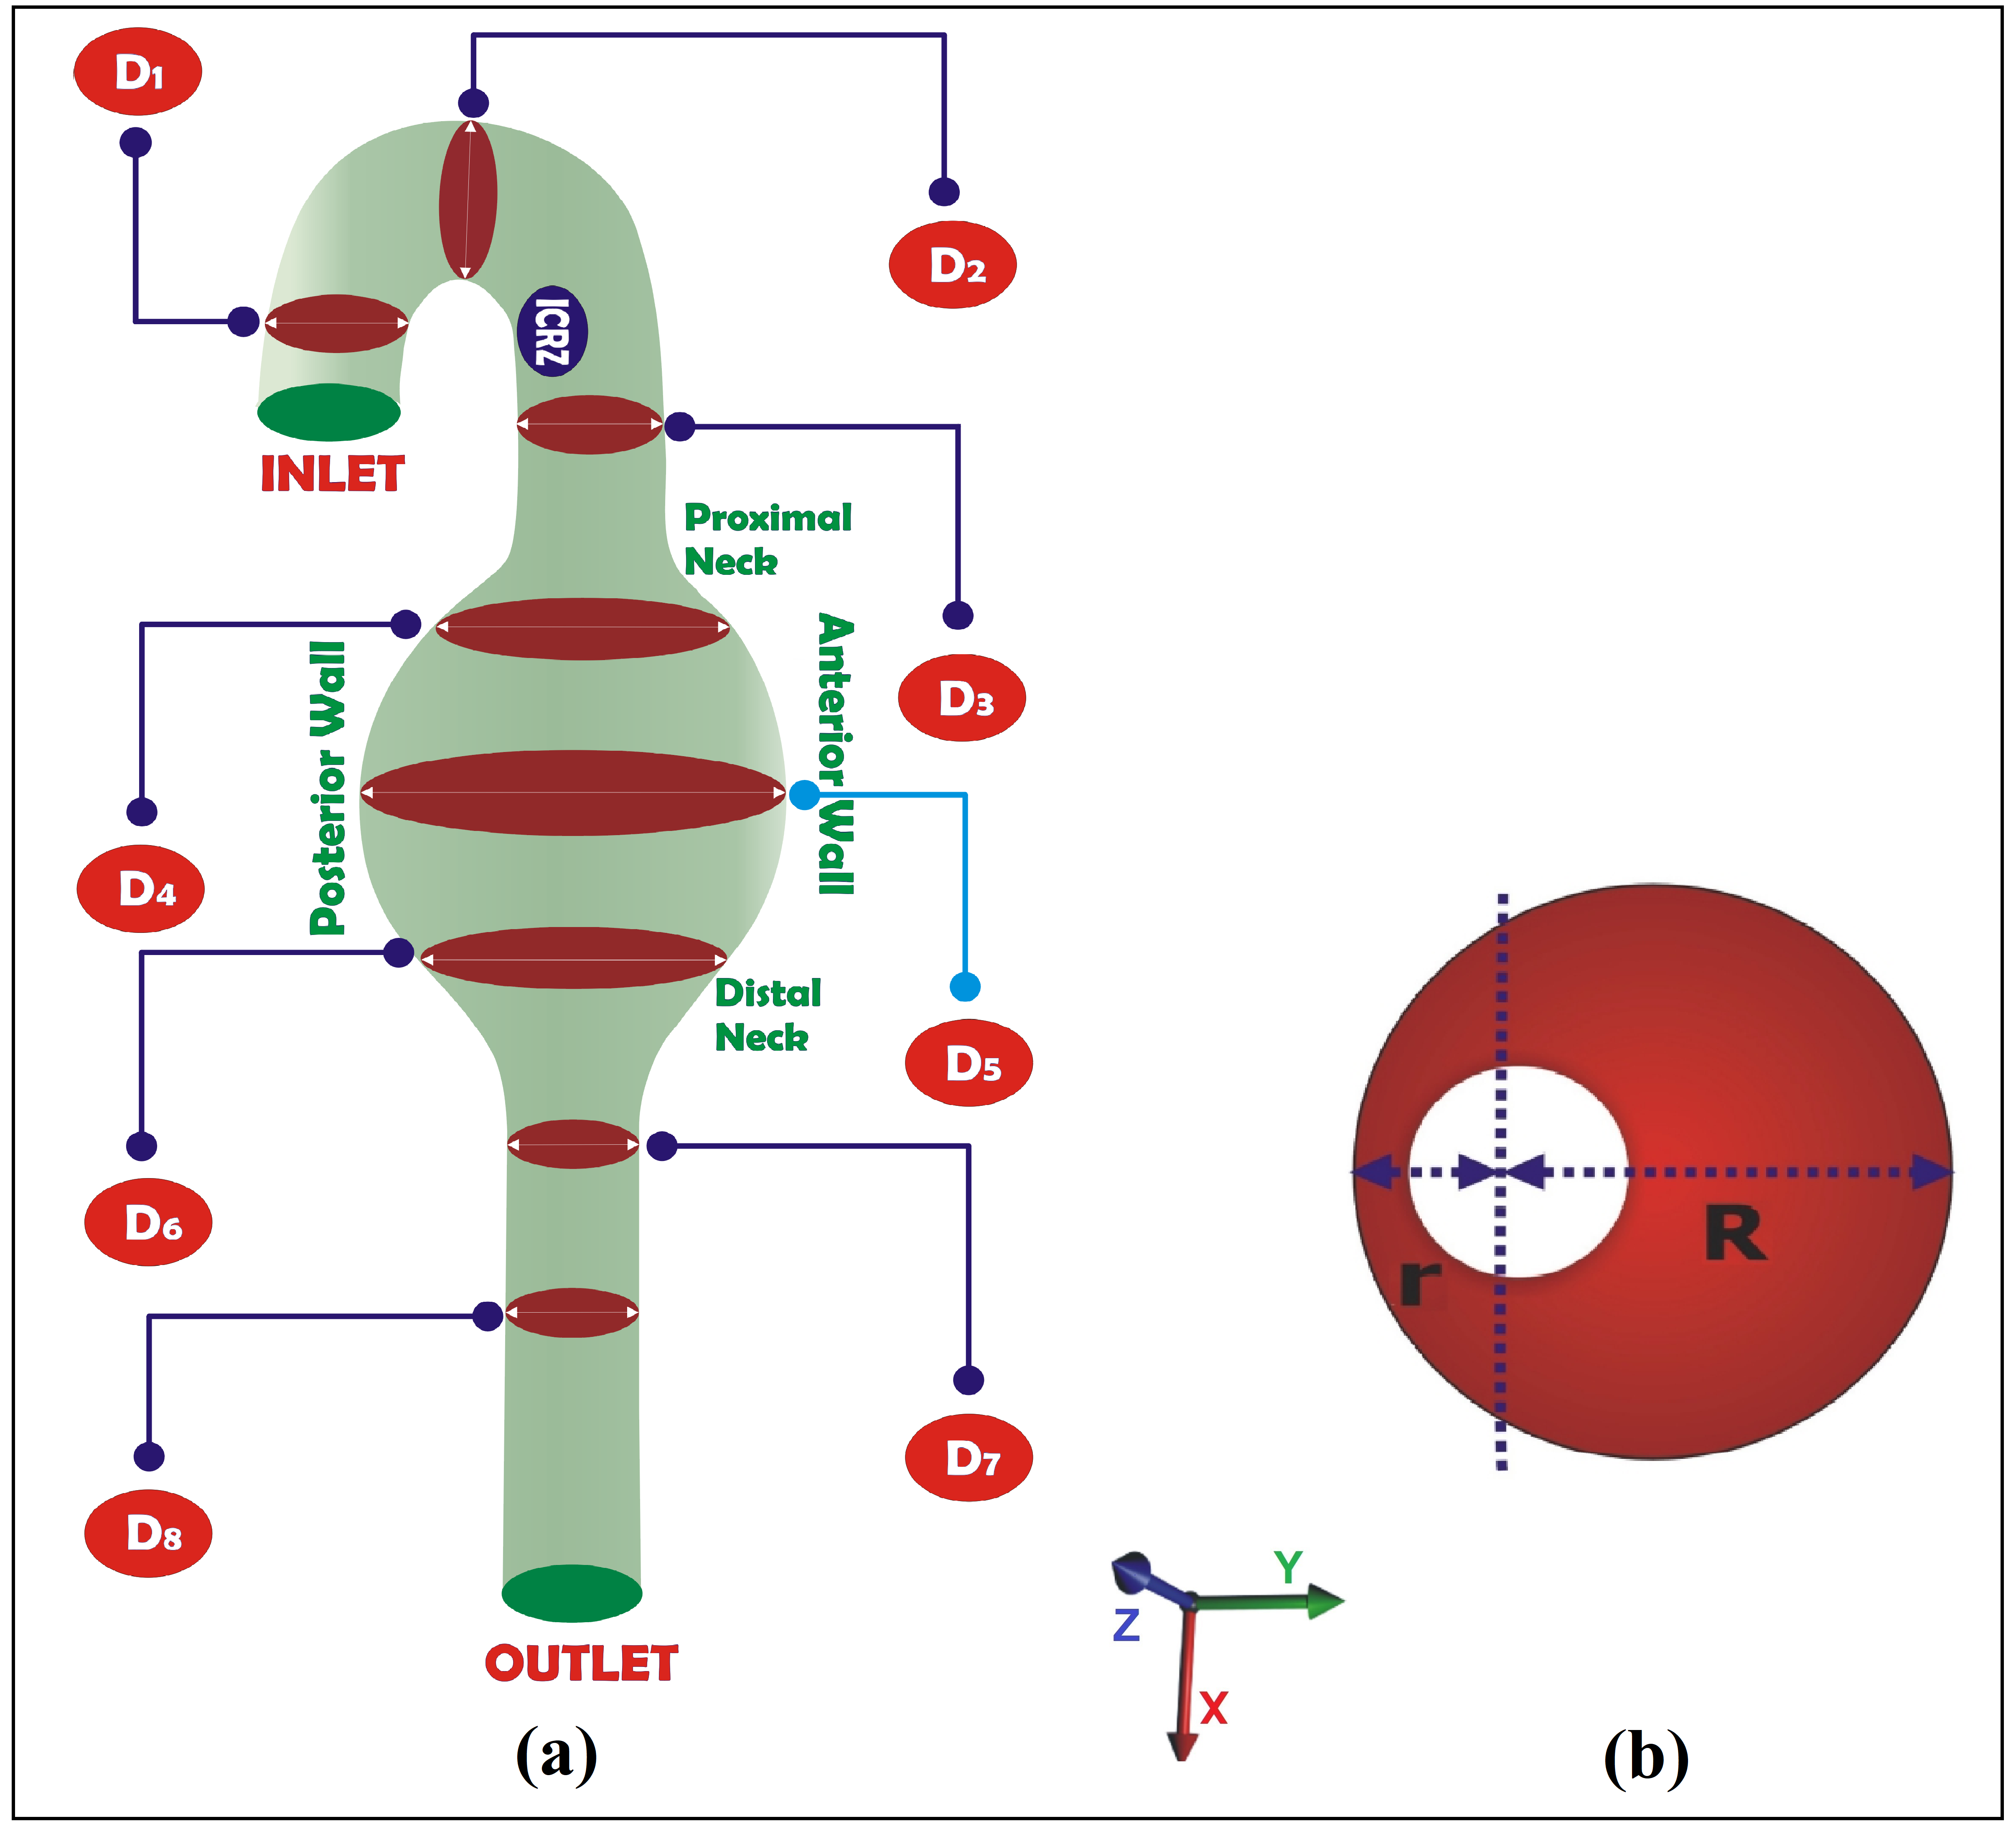
\includegraphics[width=1\textwidth, height=0.7\textheight]{Geometry.png}
         \caption{Visual depictions of (a) the three-dimensional geometry of the aneurysm and (b) the cross-sectional area of the aneurysm sac.}
         \label{fig:diagram}
     \end{figure}

     
\hspace*{\parindent} 

\subsection{\label{sec:governing_equations}Blood flow modeling and boundary conditions} 
\subsubsection{Governing equations and turbulence modeling}

The incompressible Navier--Stokes equations, which govern blood flow, are given by \cite{navier1823memoire, stokes2007theories}:
\begin{align}
    \nabla \cdot \mathbf{v} &= 0, \label{eq:cont}\\
    \rho \left( \frac{\partial \mathbf{v}}{\partial t} + (\mathbf{v} \cdot \nabla) \mathbf{v} \right) &= -\nabla p + \mu \nabla^2 \mathbf{v}, \label{eq:ns}
\end{align}
where \(\rho\) is the fluid density, \(\mathbf{v}\) the velocity vector, \(p\) the pressure, and \(\mu\) the dynamic viscosity.

For the unsteady Reynolds-averaged calculation, the instantaneous velocity will be decomposed as $\mathbf v=\mathbf V+\mathbf v'$ with $\overline{\mathbf v'}=0$, where $\mathbf V$ is the mean velocity. The Reynolds stress is closed by the Boussinesq eddy-viscosity approximation,
\begin{equation}
-\rho\overline{v_i'v_j'}=\mu_t\left(\partial_j V_i+\partial_i V_j\right)-\frac{2}{3}\rho k\delta_{ij},
\label{eq:boussinesq}
\end{equation}
where $k=\tfrac12\overline{v_i'v_i'}$ is \TKE per unit mass (m$^2$~s$^{-2}$), $\mu_t$ is dynamic eddy viscosity, and $\delta_{ij}$ is the Kronecker delta. With Eq.~\eqref{eq:boussinesq}, the Reynolds-averaged momentum equation solved for the mean velocity and pressure $P$ is
\begin{equation}
\rho\left(\frac{\partial\mathbf V}{\partial t}+(\mathbf V\cdot\nabla)\mathbf V\right)=-\nabla P+\nabla\cdot\left[(\mu+\mu_t)\left(\nabla\mathbf V+\nabla\mathbf V^{T}\right)\right]-\frac{2}{3}\nabla(\rho k),
\label{eq:urans}
\end{equation}
with $\nabla\cdot\mathbf V=0$.

\subsubsection{\texorpdfstring{\SSTcap \(k\)--\(\omega\) transition model}{SST k-omega transition model}}

The \SST \(k\)--\(\omega\) transition model was employed to account for the possible transition from laminar to turbulent flow and to capture the complex flow features associated with curvature, flow separation, and recirculation in the descending thoracic aorta. The model combines the near-wall formulation of the \(k\)--\(\omega\) model with the free-stream behavior of the \(k\)--\(\epsilon\) formulation through appropriate blending functions.

The turbulent eddy viscosity is calculated as
\begin{equation}
    \mu_t =
    \frac{a_1 \rho k}
    {\max(a_1\omega,\;SF_2)},
    \label{eq:mutt}
\end{equation}
where \(k\) is the \TKE, \(\omega\) is the specific dissipation rate, \(S\) is the magnitude of the strain-rate tensor, and \(F_2\) is the second blending function.

The transport equations for \TKE and specific dissipation rate are given by
\begin{equation}
\frac{\partial(\rho k)}{\partial t}
+\nabla\cdot(\rho k\mathbf{V})
=
\nabla\cdot
\left[
\left(\mu+\frac{\mu_t}{\sigma_k}\right)\nabla k
\right]
+P_k-D_k,
\label{eq:keqn}
\end{equation}

\begin{equation}
\frac{\partial(\rho\omega)}{\partial t}
+\nabla\cdot(\rho\omega\mathbf{V})
=
\nabla\cdot
\left[
\left(\mu+\frac{\mu_t}{\sigma_\omega}\right)\nabla\omega
\right]
+P_\omega-D_\omega
+
2(1-F_1)\rho\sigma_{\omega2}
\frac{1}{\omega}
\frac{\partial k}{\partial x_j}
\frac{\partial\omega}{\partial x_j}.
\label{eq:omegaeqn}
\end{equation}

Unlike the standard \SST \(k\)--\(\omega\) model, the transition formulation additionally solves two transport equations: one for the intermittency \(\gamma\), which varies from zero in laminar regions to unity in fully turbulent regions, and another for the transition momentum-thickness Reynolds number \(\widetilde{Re}_\theta\). These variables enable the model to predict the onset and development of boundary-layer transition based on the local flow conditions.

The blending functions \(F_1\) and \(F_2\) regulate the transition between the \(k\)--\(\omega\) and \(k\)--\(\epsilon\) formulations. \(F_1\) provides the appropriate near-wall blending, whereas \(F_2\) limits the eddy viscosity in regions where strain-rate effects become important. The distance to the nearest wall is denoted by \(y\). Thus, the \SST \(k\)--\(\omega\) transition model combines the strong near-wall behavior of the \(k\)--\(\omega\) formulation with the reduced free-stream sensitivity of the \(k\)--\(\epsilon\) formulation in the outer region of the boundary layer, while the additional intermittency and transition-Reynolds-number equations allow laminar--turbulent transition to be represented.




\subsubsection{Boundary conditions}
The pulsatile flow rate at the inlet is used in order to replicate the pulsatile nature of the blood flow in the human body. The inlet profile is expressed as:

\begin{equation}
Q(t)=
\begin{cases}
Q_0\,\sin\!\left(\dfrac{\pi\,(t-nT)}{0.35}\right)+0.05\,Q_0,
& nT \le t \le nT+0.35, \\[6pt]
0.05\,Q_0,
& nT+0.35 < t \le (n+1)T.
\end{cases}
\end{equation}


Similarly, the pulsatile outlet pressure is used at the outlet and is

\begin{equation}
P(t) =
\begin{cases} 
P_\mathrm{min} + \left(P_\mathrm{max} - P_\mathrm{min}\right) \, \sin\left(\dfrac{\pi \, (t - \, n \, T)}{0.35}\right), & nT \le t \le nT+0.35, \\
P_\mathrm{min}, & nT+0.35 < t \le (n+1)T.
\end{cases}
\end{equation}

Here $P_{\mathrm{min}}=80$~mmHg, $P_{\mathrm{max}}=120$~mmHg, $n=0,1,2,3$ indexes cardiac cycles, $T=0.8$~s, and $Q_0=2.39\times10^{-4}$~m$^3$~s$^{-1}$ is the sinusoidal amplitude. Because of the $0.05Q_0$ offset, the actual peak of the prescribed inlet flow rate is $1.05Q_0$.

{The inlet flow-rate and outlet pressure profiles that these two equations define are shown in Figure~\ref{fig:profiles}.}

\begin{figure}[!htb]
\centering
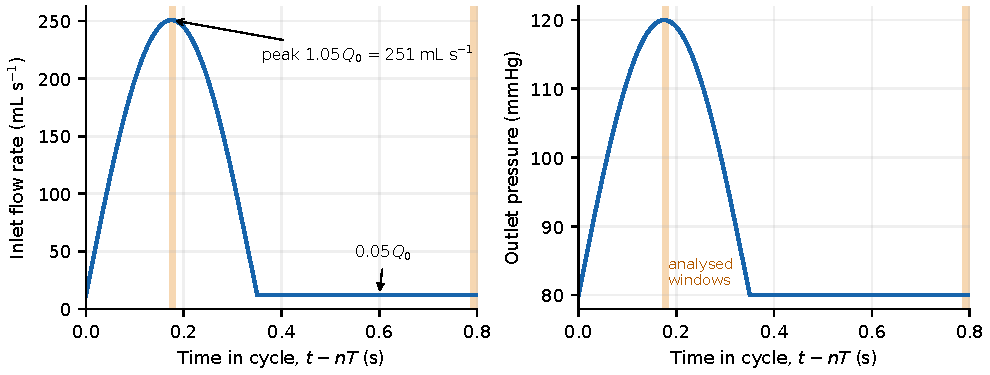
\includegraphics[width=\textwidth]{bc_profiles.pdf}
\caption{Prescribed inlet flow rate (left) and outlet pressure (right) over one cardiac cycle.}
\label{fig:profiles}
\end{figure}

At the wall no slip condition is applied.



\subsubsection{\label{sec:Hemodynamics Parameters}Hemodynamic parameters}

\hspace*{\parindent} \WSScap  denotes the tangential force per unit area applied by blood flow against the vessel wall. The \WSS for vessels \cite{potters2015volumetric} can be calculated using the formula:

\begin{align}
    \tau_w = \mu \left. \frac{\partial {u_t}}{\partial n} \right|_{n=0},
\end{align}

where \(\mu\) is the blood viscosity, \(\frac{\partial {u_t}}{\partial n}\) is the {tangential velocity gradient} in the direction \(n\) normal to the wall, and {\(u_t\) is the local tangential velocity component at the wall}.

To characterize the temporal and directional features of \WSS over a cardiac cycle, two additional metrics were computed on the aneurysm wall \cite{morbiducci2010outflow, turk2021characterization}:
\begin{equation}
\text{\TAWSScap} = \frac{1}{T} \int_{0}^{T} \left| \mathbf{WSS}(\mathbf{s},t) \right| \, dt,
\end{equation}
where $T$ is the duration of one cardiac cycle and $\mathbf{s}$ denotes a point on the vessel wall. \TAWSS  represents the magnitude of the \WSS vector averaged over time.

\TKEcap was quantified to assess the level of turbulence in the aneurysm sac, in addition to \WSS and \TAWSS. Here, \TKE represent the fluctuating components of the velocity field in the three coordinate directions. It provides an indicator of turbulence intensity and has been associated with increased flow instability and potential damage to the aneurysmal wall.

Additionally, velocity magnitudes were determined at eight predetermined cross-section planes (D1--D8) across the arterial axis and examined the spatial development of flow and its association with local vessel geometry. This was an analysis based on planes which allowed the direct correlation between morphometric parameters (diameter) and hemodynamic quantities (velocity, \TKE).


\MPScap was calculated on the inner surface of the aneurysmal wall to assess the structural response of the artery wall under pressure loading. \MPS represents the highest tensile principal stress at a given point and is commonly used in biomechanical studies as an indicator of rupture risk, because wall failure is expected when the local tensile stress exceeds the local tissue strength. The stress tensor was computed throughout the structural domain, and the spatial distribution of \MPS was analyzed to identify regions of elevated wall stress that may be more susceptible to mechanical failure.

\subsubsection{\label{CFD Simulation}\texorpdfstring{\CFDcap}{CFD} simulation}ANSYS Fluent, a commercial finite-volume solver with a pressure-based formulation, was used to solve the governing equations for mass and momentum conservation. Blood was modeled as an incompressible Newtonian fluid with density \(\rho = 1050\,\mathrm{kg\,m^{-3}}\) and dynamic viscosity \(\mu = 3.5 \times 10^{-3}\,\mathrm{Pa\,s}\).


The spatial convergence of the steady flow results was checked by performing a mesh refinement study. Prescribed flow rate was \(2.39 \times 10^{-4} \, \mathrm{m^3/s}\) and the \SST \(k\)-\(\omega\) turbulence model was used. Four different meshes (2.9~mm to 0.8~mm) were used in the testing as shown in (Table~\ref{tab:mesh_study}). The relative change, Richardson-extrapolated value and \GCI were computed between each mesh and the immediately finer mesh. The assumed second order convergence rate, $p=2$ was used in conjunction with Roache's conservative safety factor, $F_s=3.0$ for the evaluation of the \GCI. The two first refinements had relatively high \GCI values, which means that the coarser meshes were not in the range of mesh independent solution. For comparison, refinement from 1.3~mm to 0.8~mm changed the maximum aneurysmal \WSS by only 0.89\%, was Richardson extrapolated to 66.83~Pa, and had a fine-grid \GCI value of 1.63\%. Therefore, the 0.8~mm mesh was selected for the final simulations.

\begin{table}[ht!]
\centering
\setlength{\tabcolsep}{3.5pt}
\caption{Reported steady-flow fluid-mesh refinement for maximum aneurysmal \WSS. The extrapolation assumes second-order convergence.}
\label{tab:mesh_study}
\setlength{\tabcolsep}{7pt}
\begin{tabular}{cccccc}
\toprule
Element & Number of & Maximum & Relative & Richardson- & GCI$_{\rm fine}$ \\
size & elements & aneurysm & change & extrapolated & (\%) \\
(mm) & & \WSS (Pa) & (\%) & \WSS (Pa) & \\
\midrule
2.9 & 62\,261    & 47.8 & --    & --    & -- \\
1.9 & 196\,142   & 55.4 & 13.72 & 61.12 & 30.95 \\
1.3 & 578\,040   & 67.8 & 18.29 & 78.71 & 48.29 \\
0.8 & 1\,475\,430 & 67.2 & 0.89  & 66.83 & 1.63 \\
\bottomrule
\end{tabular}
\end{table}


The temporal convergence was evaluated for three different time step sizes: 0.01~s, 0.001~s, and 0.0005~s. The difference between the two smaller time steps was small, less than 2\%, and there was very good agreement in the \WSS waveforms. The time step was chosen as 0.001~s, which was found to be adequate in terms of both the level of temporal resolution and computational efficiency.

To eliminate initial transient effects and ensure a periodic steady state, the simulations were run for four consecutive cardiac cycles (\(n = 0,1,2,3\)). The percentage difference in \WSS between the third and fourth cycles was negligible (mean \(< 0.4\%\)), confirming that a periodic steady state had been reached. Accordingly, results from the third cardiac cycle were used for all subsequent analyses.



\subsubsection{Fluid--structure interaction model}

The arterial wall was modeled using ANSYS mechanical and considered as a nearly incompressible, isotropic hyperelastic material using the second-order Yeoh strain energy potential. The strain energy density function is
\begin{equation}
W = C_{10}(\bar{I}_1 - 3) + C_{20}(\bar{I}_1 - 3)^2,
\label{eq:yeoh}
\end{equation}
where \(W\) is the strain energy density, \(\bar{I}_1\) is the first deviatoric strain invariant, and \(C_{10}\) and \(C_{20}\) are material constants. The material constants were set to \(C_{10} = 98.8~\text{kPa}\) and \(C_{20} = 779.1~\text{kPa}\) \cite{zhu2025combined}. The incompressibility parameter \(D_1\) was specified as \(2.04 \times 10^{-4}~\text{kPa}^{-1}\), corresponding to a Poisson's ratio of \(\nu = 0.49\). A uniform wall thickness of 2.0~mm was assumed for all models, consistent with previous idealized \FSI studies of thoracic \AANs, and the arterial wall density was set to 1120~kg/m\(^3\).

To represent the physiological fixation of the artery, fixed boundary conditions were applied at both the inlet and outlet. The \FSI  interface was defined on the inner surface of the arterial wall to enable bidirectional coupling between the fluid and structural domains. The computational workflow is presented in Figure~\ref{fig:Flowchart}.



\begin{figure}[!ht]
  \centering
  \definecolor{cIn}{HTML}{1F6FB2}
  \definecolor{cNet}{HTML}{0E8C84}
  \definecolor{cData}{HTML}{C0392B}
  \definecolor{cPhys}{HTML}{B07A12}
  \definecolor{cPost}{HTML}{2E7D32}
  \definecolor{cOpt}{HTML}{555555}
  \resizebox{\textwidth}{!}{%
  \begin{tikzpicture}[
      font=\small,
      >={Stealth[length=2.2mm]},
      box/.style={rounded corners=2pt, draw=#1!70, line width=0.6pt, fill=#1!7,
                  align=center, inner sep=4pt, text=black, minimum width=52mm, minimum height=9mm},
      dec/.style={diamond, aspect=2.2, draw=cOpt!70, fill=cOpt!7, line width=0.6pt, inner sep=1.5pt, font=\small},
      arr/.style={->, draw=black!65, line width=0.7pt},
      lab/.style={font=\footnotesize, text=black!70},
      ilab/.style={font=\footnotesize\itshape, text=black!60},
    ]

    % ---------------------------------------------------------
    % Top: geometry
    % ---------------------------------------------------------
    \node[box=cOpt, minimum width=60mm] (geo) {\textbf{Geometry}: Twelve idealized models};

    % ---------------------------------------------------------
    % Left column: fluid
    % ---------------------------------------------------------
    \node[box=cIn, below left=8mm and -14mm of geo] (fl) {\textbf{Fluid (blood)}: ANSYS Fluent};
    \node[box=cIn, below=4mm of fl] (fmesh) {Mesh generation};
    \node[box=cIn, below=4mm of fmesh, align=center] (fset) {%
        Fluid properties and boundary conditions.\\
        Discretization method and convergence setup.};
    \node[dec, below=5mm of fset] (conv) {converged?};
    \node[box=cIn, below=6mm of conv] (fres) {Results};

    \draw[arr] (fl) -- (fmesh);
    \draw[arr] (fmesh) -- (fset);
    \draw[arr] (fset) -- (conv);
    \draw[arr] (conv) -- node[lab, right]{yes} (fres);

    \coordinate (loopx) at ($(fset.west)+(-5mm,0)$);
    \draw[arr] (conv.west) -- node[lab, above]{no} (conv.west -| loopx) |- (fset.west);

    % ---------------------------------------------------------
    % Right column: solid
    % ---------------------------------------------------------
    \node[box=cPost, below right=8mm and -14mm of geo] (so) {\textbf{Solid (wall)}: ANSYS Mechanical};
    \node[box=cPost, below=4mm of so] (smesh) {Mesh generation};
    \node[box=cPost, below=4mm of smesh, align=center] (sset) {%
        Wall properties and boundary conditions.};
    \node[box=cPost, below=4mm of sset] (sa) {Stress analysis};
    \node[box=cPost, below=4mm of sa] (sres) {Results};
    \node[box=cPost, below=4mm of sres] (end) {End};

    \draw[arr] (so) -- (smesh);
    \draw[arr] (smesh) -- (sset);
    \draw[arr] (sset) -- (sa);
    \draw[arr] (sa) -- (sres);
    \draw[arr] (sres) -- (end);

    % ---------------------------------------------------------
    % Links from geometry to both columns
    % ---------------------------------------------------------
    \draw[arr] (geo.south) -- ++(0,-3mm) -| (fl.north);
    \draw[arr] (geo.south) -- ++(0,-3mm) -| (so.north);

    % ---------------------------------------------------------
    % Wall-pressure transfer from fluid to solid
    % ---------------------------------------------------------
    \coordinate (cpx) at ($(fset.east)!0.5!(fset.east -| sa.west)$);
    \draw[arr, draw=cPhys!90, line width=0.9pt]
          (fres.east) -- (fres.east -| cpx) -- (cpx |- sa.west) -- (sa.west);
    \node[lab, text=cPhys!90!black, rotate=90, anchor=north, inner sep=1pt]
          at ($(fres.east -| cpx)!0.5!(cpx |- sa.west)$) {wall pressure};

  \end{tikzpicture}%
  }
  \caption{\CFDcap and structural workflow. The fluid problem is solved in ANSYS Fluent, and the wall pressure is transferred to the structural model in ANSYS Mechanical.}
  \label{fig:Flowchart}
\end{figure}



\section{Sparse-velocity reconstruction methods}
\label{sec:reconstruction_methods}
\subsection{Exported flow fields, instants and regions}
\label{sec:exports}
All quantitative flow results in this paper, including the reconstruction study, use whole-domain exports of the rigid-wall \CFD solutions rather than the structural calculation. For each case the exports contain every fluid node (468\,000--603\,000 interior nodes and 34\,600--41\,400 wall nodes) with velocity, static pressure, eddy viscosity $\mu_t$, $k$ and $\omega$, together with the \WSS vector on the wall nodes and the inlet and outlet faces. The mesh and node ordering are identical across the snapshots of a case, so differences between snapshots are exact nodal differences. No cell volumes, face areas or connectivity were exported, and all averages are therefore node-weighted. The near-wall node spacing differs between the two groups of models. In the aneurysmal models the interior node nearest each wall node lies a median 0.03--0.04~mm from the wall in the aneurysm zone but 0.58~mm on the rest of the wall, including the bend, whereas in the controls it lies 0.04~mm from the wall everywhere. Near-wall refinement in the aneurysmal models is therefore confined to the aneurysm zone, and quantities outside that zone, including comparisons with the controls there, depend on near-wall resolution as well as on geometry.

Snapshots exist for every case at 1.780~s and at 2.390 and 2.400~s, and for all cases except Case~2 at 1.775~s; Case~2 instead has a snapshot at 1.788~s, which completes its systolic window. Peak inflow occurs at 1.775~s, $0.175$~s into the third cycle, so 1.780~s is 5~ms after the peak, and 2.400~s is the end of the diastolic plateau of the third cycle. We use 1.780~s and 2.400~s as common systolic and diastolic instants and refer to them below as the systolic and diastolic phases. All exported fields were post-processed and plotted with Python scripts (NumPy, SciPy and Matplotlib). The earlier case-specific image exports were taken at different near-systolic times (1.775--1.815~s), and they are used only as qualitative illustrations.

Two regions are used throughout. The \emph{aneurysm zone} is the wall zone exported as the dilation for each aneurysmal case, which spans the sac and its necks. For comparisons that include the controls, the \emph{dilation segment} is the axial extent of the aneurysm zone of the axisymmetric case with the same inlet diameter, restricted to the descending branch, so that each control is evaluated over the corresponding stretch of undilated vessel. Within the straight descending segment the global $x$ axis coincides with the local downstream direction, which makes a negative $x$ velocity a meaningful indicator of reversed flow there, unlike in the curved inlet region.


\subsection{Task and information available to each method}
\label{sec:task}
Each reconstruction problem concerns one geometry and one short window of two snapshots. The systolic window is 1.775--1.780~s, with the target at 1.780~s, except for Case~2, which has no 1.775~s export and uses 1.780--1.788~s with the same target. The diastolic window is 2.390--2.400~s, with the target at 2.400~s. Given velocity at a sparse set of interior nodes at both window times, a method must recover velocity at all other interior nodes, the gauge pressure in the interior and the \WSS magnitude on the aneurysm zone at the target time. The geometry is known, so the task is reconstruction within a given anatomy rather than prediction for a new one.

Table~\ref{tab:information} lists what each method may use. Geometry comprises the coordinates of the interior nodes without their field values, the wall nodes with inward normals, and the inlet and outlet faces. Boundary information comprises the prescribed inlet velocity and the mean outlet pressure at each window time. Pressure, \WSS and velocity at unobserved nodes are never used for fitting or selection. We examine two viscosity settings. The first supplies the \CFD eddy-viscosity field $\mu_t$ and its spatial gradient, so the momentum balance uses $\mu+\mu_t$. We call this the \emph{oracle} setting because it gives the reconstruction access to closure information from the reference simulation. The second uses only the prescribed blood viscosity, $\mu=3.5\times10^{-3}$~Pa~s, with $\mu_t=0$; this is the \emph{molecular-viscosity} setting. The \CFD eddy viscosity is not measured by the sparse velocity observations. Results that use it are therefore conditional on that additional information.

\begin{table}[htbp]
\centering
\small
\caption{Information used by each method. All methods receive the same observation nodes at both window times and are scored through the same post-processing.}
\label{tab:information}
\setlength{\tabcolsep}{4pt}
\begin{tabular}{p{4.3cm}ccccc}
\toprule
Information & Linear & \RBF & \shortstack{Data\\field} & \shortstack{Continuity\\field} & \shortstack{Momentum\\\PINN} \\
\midrule
Sparse velocity at two times & \checkmark & \checkmark & \checkmark & \checkmark & \checkmark \\
Wall no-slip and inlet velocity & \checkmark & \checkmark & \checkmark & \checkmark & \checkmark \\
Outlet pressure datum & post-proc. & post-proc. & \checkmark & \checkmark & \checkmark \\
Interior node coordinates (no values) & -- & -- & -- & \checkmark & \checkmark \\
Continuity in the fit & -- & -- & -- & \checkmark & \checkmark \\
Momentum balance in the fit & -- & -- & -- & -- & \checkmark \\
\CFDcap $\mu_t$ (oracle setting) & post-proc. & post-proc. & post-proc. & post-proc. & fit + post-proc. \\
\bottomrule
\end{tabular}
\end{table}

\subsection{Observation design}
\label{sec:observations}
Velocity is observed at the interior nodes nearest to the points of a uniform Cartesian grid with spacing $\Delta$ and a random offset, keeping only grid points with an interior node within $\Delta/2$. The same nodes are observed at both window times. Sampling on a grid rather than on mesh nodes avoids oversampling the refined near-wall layers. Each grid point is, however, snapped to a mesh node, so observations next to the wall fall on the prism layers. At $\Delta=2.5$~mm, 5.6--8.5\% of the observed nodes of Cases~2--8 lie within 0.25~mm of the wall and 26--30\% within 1~mm, the closest at 0.03~mm, whereas a 2.5~mm imaging voxel would return an average over its volume. The design is therefore point sampling on a grid rather than voxel sampling. Every method receives the same observations, so the comparison between methods is not affected, but the absolute \WSS errors are optimistic relative to imaging data; Section~\ref{sec:nearwall} quantifies this by removing the near-wall observations. The primary spacing $\Delta=2.5$~mm observes 1.27--1.36\% of the interior nodes per time (5\,970--8\,205 nodes), and the secondary spacings of 1.5 and 4.0~mm observe 5.4--5.8\% and 0.34--0.37\%. The observed values are noise-free \CFD values at mesh nodes. A random 10\% of the observed nodes is withheld from fitting and used only for model selection and monitoring. Each draw $s$ fixes both the grid offset and the network initialization, draws are paired across methods, and the observed node indices are stored.


\subsection{Space-time neural fields and physics constraints}
\label{sec:field}
We use a space-time neural field to represent each short flow window. The confirmation method is a continuity-constrained field followed by physics-based post-processing, in which the network reconstructs velocity and separate calculations recover pressure and \WSS. We refer to this method as the continuity field. Its divergence penalty is a physical constraint, but it does not enforce the momentum balance during fitting. We use the term \emph{momentum \PINN} for the separate arms, tested only on the two development geometries, that also penalize the momentum residual. 

All neural arms share the same architecture, which maps position and time to velocity and pressure, $(\mathbf x,t)\mapsto(\mathbf u_\theta,p_\theta)$. Coordinates are scaled as $\mathbf x_s=(\mathbf x-\mathbf x_c)/L$, where $\mathbf x_c$ is the centroid of the interior nodes and $L$ is half the largest extent of the domain, and time is mapped to $t_s\in[-1,1]$ across the window. Velocity is scaled by $U$, the 99.5th percentile of observed speed at the target time, and pressure by $\rho U^2$. The input is $[\sin(2\pi\mathbf B^{\mathsf T}\mathbf x_s),\cos(2\pi\mathbf B^{\mathsf T}\mathbf x_s),\mathbf x_s,t_s]$, where $\mathbf B\in\mathbb R^{3\times64}$ holds Gaussian Fourier features with a \SD of 2~\cite{tancik2020fourier}, followed by six fully connected layers of width 256 with SiLU activations and a linear output of four scaled quantities (about 360\,000 parameters) (Figure~\ref{fig:network}).

\begin{figure}[!t]
  \centering
  \definecolor{cIn}{HTML}{1F6FB2}
  \definecolor{cEnc}{HTML}{6A4C93}
  \definecolor{cNet}{HTML}{0E8C84}
  \definecolor{cData}{HTML}{C0392B}
  \definecolor{cPhys}{HTML}{B07A12}
  \definecolor{cBC}{HTML}{2E7D32}
  \definecolor{cOpt}{HTML}{555555}
  \resizebox{\textwidth}{!}{%
  \begin{tikzpicture}[
      font=\small,
      >={Stealth[length=2.2mm]},
      box/.style={rounded corners=2pt, draw=#1!70, line width=0.6pt, fill=#1!7,
                  align=center, inner sep=3.5pt, text=black},
      box/.default=black,
      inp/.style={box=cIn,  minimum width=24mm, minimum height=9mm},
      enc/.style={box=cEnc, minimum width=30mm, minimum height=10mm},
      cat/.style={draw=black!55, fill=black!6, circle, inner sep=1.5pt, minimum size=13mm, align=center},
      outn/.style={circle, draw=#1!75, fill=#1!16, line width=0.6pt, minimum size=7.5mm,
                  inner sep=0pt, font=\footnotesize},
      loss/.style={box=#1, minimum width=40mm, minimum height=12mm},
      opt/.style={box=cOpt, minimum width=36mm, minimum height=10mm},
      neuron/.style={circle, draw=cNet!70, fill=cNet!12, minimum size=3.4mm, inner sep=0pt},
      edge/.style={draw=cNet!35, line width=0.25pt},
      arr/.style={->, draw=black!65, line width=0.7pt},
      bus/.style={draw=black!60, line width=0.7pt},
      lab/.style={font=\footnotesize, text=black!70},
      ilab/.style={font=\footnotesize\itshape, text=black!60},
    ]
    \node[inp] (x) {$\mathbf{x}=(x,y,z)$};
    \node[inp, below=12mm of x] (t) {$t\in[t_o,t_\star]$};
    \node[lab, left=1mm of x] (lx) {position};
    \node[lab, left=1mm of t] (lt) {time};
    \node[enc, right=10mm of x] (fF) {Fourier features $\gamma(\mathbf{x}_s)$\\{\footnotesize 64 frequencies, $\sigma=2$}};
    \node[enc, right=10mm of t] (ts) {window scaling\\{\footnotesize $t_s\in[-1,1]$}};
    \coordinate (mid) at ($(fF.east)!0.5!(ts.east)$);
    \node[cat, right=9mm of mid] (cat) {\scriptsize concat\\[-1pt]\scriptsize $[\gamma,\mathbf{x}_s,t_s]$};
    \draw[arr] (x) -- (fF);
    \draw[arr] (t) -- (ts);
    \draw[arr] (fF.east) -- ([yshift= 2mm]cat.west);
    \draw[arr] (ts.east) -- ([yshift=-2mm]cat.west);

    \coordinate (netorg) at ($(cat.east)+(27mm,0)$);
    \begin{scope}[shift={(netorg)}]
      \node[rounded corners=3pt, draw=cNet!70, fill=white, minimum width=38mm, minimum height=27mm] (mlp) {};
      \foreach \i in {1,2,3}\node[neuron] (a\i) at (-15mm, {(\i-2)*6mm}) {};
      \foreach \i in {1,2,3,4}\node[neuron] (b\i) at (-5mm, {(\i-2.5)*5mm}) {};
      \foreach \i in {1,2,3,4}\node[neuron] (c\i) at (5mm,  {(\i-2.5)*5mm}) {};
      \node[neuron] (d1) at (15mm,0) {};
      \foreach \i in {1,2,3}\foreach \j in {1,2,3,4}\draw[edge] (a\i)--(b\j);
      \foreach \i in {1,2,3,4}\foreach \j in {1,2,3,4}\draw[edge] (b\i)--(c\j);
      \foreach \i in {1,2,3,4}\draw[edge] (c\i)--(d1);
    \end{scope}
    \node[ilab, text=cNet!80, below=1.5mm of mlp] (mlplab) {6 layers $\times$ 256 units, SiLU};
    \draw[arr] (cat.east) -- (a2);

    \node[outn=cIn, right=15mm of mlp, yshift=11.5mm] (ou) {$u$};
    \node[outn=cIn, below=2.2mm of ou] (ov) {$v$};
    \node[outn=cIn, below=2.2mm of ov] (ow) {$w$};
    \node[outn=cPhys, below=2.2mm of ow] (op) {$p$};
    \foreach \o in {ou,ov,ow,op}{\draw[arr] (d1) -- (\o);}
    \draw[decorate, decoration={brace, amplitude=3pt, raise=1pt}, draw=black!50, line width=0.5pt]
      ($(ou.east)+(1.5mm,0)$) -- ($(ow.east)+(1.5mm,0)$);
    \node[lab, anchor=west] (lvel) at ($(ov.east)+(5.5mm,0)$) {velocity};
    \node[lab, anchor=west] (lpre) at (lvel.west |- op) {pressure};

    \begin{scope}[on background layer]
      \node[rounded corners=4pt, draw=black!40, fill=black!1.5,
            fit=(lx)(lt)(x)(t)(fF)(ts)(cat)(mlp)(mlplab)(ou)(op)(lvel)(lpre), inner sep=5mm] (net) {};
    \end{scope}
    \node[ilab, anchor=south west, text=black!65] at ($(net.north west)+(1.5mm,0.8mm)$)
         {Network $f_\theta(\mathbf{x},t)$, fitted separately for each case and window};

    \node[loss=cPhys] (phys) at ($(net.south)+(0,-16mm)$)
         {\textbf{Physics}, weight $w=0.01$\\continuity $\nabla\!\cdot\mathbf{u}$\\{\footnotesize\color{black!60}momentum \PINNs: + momentum residual}};
    \node[loss=cData, left=10mm of phys] (data)
         {\textbf{Data}\\$\mathbf{u}$ at observed nodes, $t_o$ and $t_\star$};
    \node[loss=cBC, right=10mm of phys] (bc)
         {\textbf{Boundary}\\no-slip, inlet $\mathbf{u}$, outlet datum};
    \coordinate (busL) at ($(net.south)+(0,-6mm)$);
    \draw[bus] (net.south) -- (busL);
    \node[ilab, anchor=south west, text=black!70] at ($(net.south)+(1.8mm,-1mm)$) {predictions};
    \draw[bus] (busL) -| (data.north);
    \draw[arr] (busL) -- (phys.north);
    \draw[bus] (busL) -| (bc.north);
    \draw[arr] ($(data.north)+(0,2mm)$)--(data.north);
    \draw[arr] ($(bc.north)+(0,2mm)$)--(bc.north);

    \node[opt, minimum width=48mm] (sum) at ($(phys.south)+(0,-11mm)$) {$\mathcal L=\mathcal L_{\rm data}+\mathcal L_{\rm bc}+w\,\mathcal L_{\rm phys}$};
    \node[opt, below=6mm of sum] (adam) {Adam, lr $10^{-3}\!\to\!10^{-5}$ (cosine),\\20\,000 steps, gradient clipping};
    \draw[arr] (data.south) |- (sum.west);
    \draw[arr] (phys.south) -- (sum.north);
    \draw[arr] (bc.south) |- (sum.east);
    \draw[arr] (sum.south) -- (adam.north);
    \coordinate (fbmid) at ([xshift=7mm]net.east);
    \coordinate (fbbot) at (fbmid |- adam.east);
    \draw[arr, dashed, draw=black!55] (adam.east) -- (fbbot)
       -- node[lab, pos=0.55, right]{$\nabla_\theta$} (fbmid) -- (net.east);
  \end{tikzpicture}%
  }
  \caption{Space-time neural field. Fourier-encoded position and scaled time pass through a fully connected network to velocity and pressure, fitted to the observed velocity and the boundary conditions. The continuity arm adds a divergence penalty; the momentum residual (gray) was used only by the momentum \PINNs tested on the two development geometries.}
  \label{fig:network}
\end{figure}


The loss combines data and boundary terms with an optional physics term,
\begin{equation}
\mathcal L=\mathcal L_{\rm obs}+\mathcal L_{\rm wall}+\mathcal L_{\rm in}+\mathcal L_{\rm out}+w\,\mathcal L_{\rm phys},
\label{eq:loss}
\end{equation}
where $\mathcal L_{\rm obs}$ is the mean squared velocity misfit at the observed nodes at both times, $\mathcal L_{\rm wall}$ penalizes velocity at wall nodes at random times in the window, $\mathcal L_{\rm in}$ penalizes the misfit to the prescribed inlet velocity at each window time, and $\mathcal L_{\rm out}$ penalizes the squared mean of $p_\theta$ on the outlet face, which fixes the pressure datum. Four arms differ only in $\mathcal L_{\rm phys}$. The \emph{data} arm has none. The \emph{continuity} arm uses the mean squared divergence $(\nabla\cdot\mathbf u_\theta)^2$ at interior nodes drawn at random times. The \emph{steady} and \emph{unsteady} momentum arms add the mean squared residual of
\begin{equation}
\rho\,\partial_t\mathbf u+\rho(\mathbf u\cdot\nabla)\mathbf u
+\nabla p-\nabla\cdot\left[(\mu+\mu_t)
(\nabla\mathbf u+\nabla\mathbf u^{\mathsf T})\right]=\mathbf 0,
\label{eq:momentum}
\end{equation}
without the time term in the steady arm, with $\mu_t$ interpolated linearly in time between the two snapshots in the oracle setting and set to zero in the molecular setting. Derivatives are taken by automatic differentiation, and the variable-viscosity divergence retains the gradient of $\mu_t$. Equation~\eqref{eq:momentum} has no separate $2\rho k/3$ term because the exported \CFD pressure satisfies the momentum balance better without it (Section~\ref{sec:reference_results}), indicating that the isotropic turbulent stress is already contained in the exported pressure.

Each step draws 4096 observations, 4096 collocation nodes, 2048 wall nodes, 512 inlet nodes per time and 256 outlet nodes per time. Training uses Adam with a learning rate of $10^{-3}$, cosine decay to $10^{-5}$ over 20\,000 steps and gradient-norm clipping at 1. There is no early stopping, and the last iterate is scored. The physics weight $w$ was chosen for each arm from $\{0.01,0.1,1\}$ on Case~1 at systole by the error on the withheld observations and then frozen. That error increased with $w$ in every arm, so $w=0.01$ was used throughout. On one NVIDIA Quadro RTX 8000 shared with other jobs, a 20\,000-step fit took a median of 23~min for the continuity arm and 17~min for the data arm.

\subsection{Interpolation comparators}
\label{sec:interpolation}
The comparators interpolate the same observations, with zero velocity at the wall nodes and the prescribed inlet velocity added as sources, separately at each window time. \emph{Linear} interpolation uses the Delaunay triangulation of the sources, with the nearest source used outside its hull. \emph{\RBF} interpolation uses a local thin-plate-spline \RBF with a linear polynomial on the 64 nearest sources, which is widened to 128 sources only where a neighborhood is coplanar and the local system is singular. These settings were fixed before the development test and are the prespecified comparator. Two further comparators were added after the confirmatory verdict as robustness checks. The \emph{tuned \RBF} selects the kernel (thin-plate spline, cubic or quintic), the neighborhood size (32--256) and the smoothing parameter ($0$--$10^{-2}$) by the error on the withheld observations. The \emph{space-time \RBF} fits one interpolant over $(\mathbf x, c\,t)$ through both snapshots, with the time scale $c\in\{0,0.5,2,8\}$~m~s$^{-1}$, the kernel and the neighborhood size chosen on the same withheld observations.

\subsection{Shared post-processing}
\label{sec:postprocessing}
Every reconstruction, including the complete \CFD velocity used as a reference, is converted to pressure and \WSS by the same steps (Figure~\ref{fig:pipeline}). The reconstructed velocity is first sampled at the \CFD nodes. Spatial gradients are computed by weighted least squares on the 40 nearest nodes with inverse-square-distance weights, with zero velocity imposed at the wall nodes. The momentum balance then gives a target pressure gradient,
\begin{equation}
\mathbf f=-\rho\,\frac{\mathbf u(t_\star)-\mathbf u(t_o)}{t_\star-t_o}
-\rho(\mathbf u\cdot\nabla)\mathbf u
+\nabla\cdot\left[(\mu+\mu_t)(\nabla\mathbf u+\nabla\mathbf u^{\mathsf T})\right],
\label{eq:pressure_rhs}
\end{equation}
evaluated at the target time $t_\star$, where $t_o$ is the other window time. The gauge pressure is the least-squares solution of $\nabla_h p=\mathbf f$ on the interior nodes more than 1~mm from the wall, with the mean pressure over nodes beyond $x=0.130$~m set to zero, computed with LSQR. Near-wall nodes are excluded because the prism-layer stencils are poorly conditioned. Dropping the first term of Eq.~\eqref{eq:pressure_rhs} gives the steady form, and setting $\mu_t=0$ gives the molecular form. All four combinations are reported, and the unsteady form with oracle $\mu_t$ is the prespecified pressure endpoint. The steady form of Eq.~\eqref{eq:pressure_rhs} is the standard pressure-gradient route of velocity-based relative-pressure estimation~\cite{bertoglio2018relative}.

\WSScap is estimated at each aneurysm-zone wall node $\mathbf x_w$ with inward unit normal $\mathbf n$ from the tangential velocity $\mathbf u_t$ at two distances inside the lumen,
\begin{equation}
\boldsymbol\tau_w\approx\mu\,\frac{4\,\mathbf u_t(\mathbf x_w+h\mathbf n)-\mathbf u_t(\mathbf x_w+2h\mathbf n)}{2h},
\label{eq:wss_estimate}
\end{equation}
which is second-order accurate for a no-slip wall, with $\mathbf u_t$ obtained by linear interpolation of the nodal velocity. The prespecified distance is $h=0.25$~mm, and results at 0.1 and 0.5~mm are reported only as an oracle sensitivity. In the aneurysm zone the interior node nearest the wall lies a median 0.03--0.04~mm from it, so Eq.~\eqref{eq:wss_estimate} is informative there. Outside the aneurysm zone that distance is 0.58~mm, and even the complete \CFD velocity reproduces the exported \WSS there only to a relative error of 0.46--0.68, so \WSS outside the aneurysm zone is not used as a target.


\begin{figure}[!t]
  \centering
  \definecolor{cIn}{HTML}{1F6FB2}
  \definecolor{cNet}{HTML}{0E8C84}
  \definecolor{cData}{HTML}{C0392B}
  \definecolor{cPhys}{HTML}{B07A12}
  \definecolor{cPost}{HTML}{2E7D32}
  \definecolor{cOpt}{HTML}{555555}
  % outline of an idealized aneurysmal segment, used by the pictograms below
  \def\vesselpath{(-1.1,0.22) -- (-0.45,0.22) .. controls (-0.25,0.62) and (0.25,0.62) .. (0.45,0.22)
    -- (1.1,0.22) -- (1.1,-0.22) -- (0.45,-0.22) .. controls (0.25,-0.62) and (-0.25,-0.62) .. (-0.45,-0.22)
    -- (-1.1,-0.22) -- cycle}
  \resizebox{\textwidth}{!}{%
  \begin{tikzpicture}[
      font=\small,
      >={Stealth[length=2.2mm]},
      card/.style={rounded corners=3pt, draw=#1!70, line width=0.6pt, fill=#1!6},
      ttl/.style={font=\small\bfseries, text=black, align=center},
      sub/.style={font=\footnotesize, text=black!72, align=center},
      arr/.style={->, draw=black!60, line width=0.7pt},
      ln/.style={draw=black!60, line width=0.7pt},
      step/.style={circle, fill=#1, text=white, font=\footnotesize\bfseries, inner sep=0pt, minimum size=4.8mm},
      steplab/.style={font=\small\bfseries, text=black!75, anchor=west},
      % ---------- pictograms ----------
      obsicon/.pic={
        \draw[cIn!70, line width=0.6pt, fill=white] \vesselpath;
        \foreach \x in {-0.9,-0.6,...,0.95}{\fill[cIn] (\x,0.1) circle (0.045); \fill[cIn] (\x,-0.1) circle (0.045);}
        \foreach \x in {-0.2,0.1}{\fill[cIn] (\x,0.36) circle (0.045); \fill[cIn] (\x,-0.36) circle (0.045);}
      },
      linicon/.pic={
        \draw[cOpt!80, line width=0.45pt, fill=cOpt!10]
          (0,0) -- (0.5,0.08) -- (0.22,0.45) -- cycle (0.5,0.08) -- (0.78,0.46) -- (0.22,0.45)
          (0,0) -- (-0.28,0.36) -- (0.22,0.45);
        \foreach \p in {(0,0),(0.5,0.08),(0.22,0.45),(0.78,0.46),(-0.28,0.36)}{\fill[cIn] \p circle (0.05);}
      },
      rbficon/.pic={
        \draw[cOpt!45, line width=0.4pt] (-0.45,0) -- (0.85,0);
        \draw[cOpt!85, line width=0.7pt, domain=-0.45:0.85, samples=50, smooth]
          plot (\x,{0.45*exp(-((\x+0.02)^2)/0.03)+0.28*exp(-((\x-0.45)^2)/0.02)});
        \fill[cIn] (-0.02,0.45) circle (0.05); \fill[cIn] (0.45,0.29) circle (0.05);
      },
      nnicon/.pic={
        \foreach \a in {-0.22,0,0.22}{\foreach \b in {-0.33,-0.11,0.11,0.33}{\draw[cNet!35, line width=0.3pt] (0,\a) -- (0.4,\b);}}
        \foreach \b in {-0.33,-0.11,0.11,0.33}{\draw[cNet!35, line width=0.3pt] (0.4,\b) -- (0.8,0.1); \draw[cNet!35, line width=0.3pt] (0.4,\b) -- (0.8,-0.1);}
        \foreach \a in {-0.22,0,0.22}{\fill[cNet] (0,\a) circle (0.05);}
        \foreach \b in {-0.33,-0.11,0.11,0.33}{\fill[cNet] (0.4,\b) circle (0.05);}
        \fill[cNet] (0.8,0.1) circle (0.05); \fill[cNet] (0.8,-0.1) circle (0.05);
      },
      velicon/.pic={
        \draw[cIn!70, line width=0.6pt, fill=white] \vesselpath;
        \foreach \x in {-0.95,-0.65,0.45,0.75}{\draw[->, >={Stealth[length=0.8mm]}, cIn, line width=0.45pt] (\x,0) -- ++(0.24,0);}
        \draw[->, >={Stealth[length=0.8mm]}, cIn, line width=0.45pt] (-0.3,0) -- ++(0.55,0);
        \draw[->, >={Stealth[length=0.8mm]}, cData!80, line width=0.45pt] (0.12,0.36) -- ++(-0.22,0);
        \draw[->, >={Stealth[length=0.8mm]}, cData!80, line width=0.45pt] (0.12,-0.36) -- ++(-0.22,0);
      },
      cfdicon/.pic={
        \draw[cOpt!60, line width=0.6pt, fill=white] \vesselpath;
        \foreach \y in {-0.12,0,0.12}{\draw[cOpt!55, line width=0.35pt] (-1.05,\y) .. controls (-0.3,\y) and (0.3,\y) .. (1.05,\y);}
        \draw[cOpt!55, line width=0.35pt] (-0.15,0.3) ellipse (0.18 and 0.08);
        \draw[cOpt!55, line width=0.35pt] (-0.15,-0.3) ellipse (0.18 and 0.08);
      },
      presicon/.pic={
        \shade[left color=cData!60, right color=cIn!45] \vesselpath;
        \draw[black!45, line width=0.5pt] \vesselpath;
        \node[font=\tiny\bfseries, text=white] at (-0.72,0) {$+$};
        \node[font=\tiny\bfseries, text=black!70] at (0.72,0) {$-$};
      },
      wssicon/.pic={
        \foreach \x in {-0.5,-0.36,...,0.62}{\draw[black!45, line width=0.35pt] (\x,0) -- ++(-0.11,-0.11);}
        \draw[black!70, line width=0.7pt] (-0.62,0) -- (0.62,0);
        \draw[cPost, line width=0.6pt, domain=0:0.62, samples=20, smooth] plot ({-0.45+0.9*(1-(1-\x/0.62)^2)},\x);
        \foreach \y in {0.12,0.24,0.36,0.48}{\draw[->, >={Stealth[length=0.7mm]}, cPost!70, line width=0.35pt] (-0.45,\y) -- ({-0.45+0.9*(1-(1-\y/0.62)^2)},\y);}
        \fill[cData] (-0.45,0.15) circle (0.04); \fill[cData] (-0.45,0.3) circle (0.04);
        \node[font=\tiny, text=cData, anchor=east, inner sep=1pt] at (-0.47,0.15) {$h$};
        \node[font=\tiny, text=cData, anchor=east, inner sep=1pt] at (-0.47,0.3) {$2h$};
      },
      scoreicon/.pic={
        \draw[black!50, line width=0.4pt] (-0.5,0) -- (0.6,0);
        \fill[cData!75] (-0.4,0) rectangle ++(0.22,0.18);
        \fill[cOpt!55] (-0.12,0) rectangle ++(0.22,0.46);
        \fill[cData!75] (0.16,0) rectangle ++(0.22,0.12);
        \fill[cOpt!55] (0.44,0) rectangle ++(0.14,0.36);
      },
    ]

    % ---------------- stage 1: observations ----------------
    \node[card=cIn, minimum width=36mm, minimum height=46mm] (obs) at (0,0) {};
    \node[ttl] at ($(obs.north)+(0,-4.5mm)$) {Sparse velocity};
    \pic[scale=1.25] at ($(obs.center)+(0,5mm)$) {obsicon};
    \node[sub] at ($(obs.center)+(0,-9.5mm)$) {$\sim$1.3\% of interior\\nodes at $t_o$ and $t_\star$\\[2pt]+ wall, inlet and\\outlet conditions};

    % ---------------- stage 2: reconstruction ----------------
    \def\cw{50mm}
    \node[card=cOpt, minimum width=\cw, minimum height=14mm] (lin) at (56mm,18mm) {};
    \pic[scale=0.95] at ($(lin.west)+(6.5mm,-2mm)$) {linicon};
    \node[anchor=west, align=left, font=\small] at ($(lin.west)+(16mm,0)$) {\textbf{Linear}\\{\footnotesize\color{black!70}each time separately}};

    \node[card=cOpt, minimum width=\cw, minimum height=14mm] (rbf) at (56mm,0) {};
    \pic[scale=0.95] at ($(rbf.west)+(6mm,-2mm)$) {rbficon};
    \node[anchor=west, align=left, font=\small] at ($(rbf.west)+(16mm,0)$) {\textbf{\RBF}\\{\footnotesize\color{black!70}each time separately}};

    \node[card=cNet, minimum width=\cw, minimum height=14mm] (nf) at (56mm,-18mm) {};
    \pic[scale=0.95] at ($(nf.west)+(4.5mm,0)$) {nnicon};
    \node[anchor=west, align=left, font=\small] at ($(nf.west)+(16mm,0)$) {\textbf{Neural field}\\{\footnotesize\color{black!70}both times jointly}};

    \node[card=cOpt, dashed, minimum width=\cw, minimum height=14mm] (ref) at (56mm,-39mm) {};
    \pic[scale=0.62] at ($(ref.west)+(8.5mm,0)$) {cfdicon};
    \node[anchor=west, align=left, font=\small] at ($(ref.west)+(16mm,0)$) {\textbf{Complete \CFD}\\{\footnotesize\color{black!70}reference floor}};

    \coordinate (split) at ($(obs.east)+(6mm,0)$);
    \draw[ln] (obs.east) -- (split);
    \draw[arr] (split) |- (lin.west);
    \draw[arr] (split) -- (rbf.west);
    \draw[arr] (split) |- (nf.west);

    % ---------------- stage 3: velocity on the CFD nodes ----------------
    \node[card=cIn, minimum width=34mm, minimum height=34mm] (nod) at (112mm,0) {};
    \node[ttl] at ($(nod.north)+(0,-4.5mm)$) {Velocity on\\\CFD nodes};
    \pic[scale=1.1] at ($(nod.center)+(0,-2mm)$) {velicon};
    \node[sub] at ($(nod.center)+(0,-11mm)$) {$\mathbf u(t_o)$,\ $\mathbf u(t_\star)$};

    \coordinate (join) at ($(nod.west)+(-7mm,0)$);
    \draw[ln] (lin.east) -| (join);
    \draw[ln] (nf.east) -| (join);
    \draw[ln] (rbf.east) -- (join);
    \draw[arr] (join) -- (nod.west);
    \draw[arr, dashed, draw=black!50] (ref.east) -| (nod.south);

    % ---------------- stage 4: shared post-processing ----------------
    \node[card=cPost, minimum width=64mm, minimum height=19mm] (pr) at (178mm,13mm) {};
    \pic[scale=0.72] at ($(pr.west)+(10mm,0)$) {presicon};
    \node[anchor=west, align=left, font=\small] at ($(pr.west)+(19mm,0)$) {\textbf{Pressure}\\{\footnotesize\color{black!70}least squares, $\nabla p=\mathbf f$}\\{\footnotesize\color{black!70}nodes $>1$~mm from wall}};

    \node[card=cPost, minimum width=64mm, minimum height=19mm] (ws) at (178mm,-13mm) {};
    \pic[scale=1.1] at ($(ws.west)+(10mm,-3.5mm)$) {wssicon};
    \node[anchor=west, align=left, font=\small] at ($(ws.west)+(19mm,0)$) {\textbf{\WSScap}\\{\footnotesize\color{black!70}one-sided difference}\\{\footnotesize\color{black!70}$h=0.25$~mm, aneurysm zone}};

    \node[card=cPhys, minimum width=64mm, minimum height=11mm, font=\footnotesize, align=center] (info) at (178mm,35mm)
      {$\partial_t\mathbf u\approx[\mathbf u(t_\star)-\mathbf u(t_o)]/(t_\star-t_o)$\\eddy viscosity $\mu_t$: \CFD oracle or $0$};
    \draw[arr, draw=cPhys!80] (info) -- (pr);

    \begin{scope}[on background layer]
      \node[rounded corners=5pt, draw=cPost!45, dashed, fill=cPost!2, fit=(pr)(ws)(info), inner sep=3.5mm] (grp) {};
    \end{scope}
    \node[font=\footnotesize\itshape, text=cPost!80!black, anchor=north] at (grp.south) {identical for every method};

    \coordinate (fork) at ($(nod.east)+(6mm,0)$);
    \draw[ln] (nod.east) -- (fork);
    \draw[arr] (fork) |- (pr.west);
    \draw[arr] (fork) |- (ws.west);

    % ---------------- stage 5: scores ----------------
    \node[card=cData, minimum width=32mm, minimum height=38mm] (sc) at (242mm,0) {};
    \node[ttl] at ($(sc.north)+(0,-4.5mm)$) {Scores};
    \node[sub] at ($(sc.north)+(0,-9.5mm)$) {against hidden \CFD};
    \pic[scale=1.2] at ($(sc.center)+(0,-2.5mm)$) {scoreicon};
    \node[sub] at ($(sc.center)+(0,-10.5mm)$) {velocity, pressure,\\\WSS};
    \draw[arr] (pr.east) -- ++(6mm,0) |- ([yshift=6mm]sc.west);
    \draw[arr] (ws.east) -- ++(6mm,0) |- ([yshift=-6mm]sc.west);
    \draw[arr, dashed, draw=black!50] (fork) -- (fork |- 0,-39mm) -- node[pos=0.6, above, font=\footnotesize, text=black!65] {velocity at unobserved nodes} (sc.south |- 0,-39mm) -- (sc.south);

    % ---------------- stage headers ----------------
    \foreach \n/\x/\c/\t in {1/obs/cIn/Observe, 2/lin/cOpt/Reconstruct, 3/nod/cIn/Sample, 4/grp/cPost/Post-process, 5/sc/cData/Score}{
      \node[steplab, anchor=center] (t\n) at ($(\x.center |- 0,50mm)+(2.6mm,0)$) {\t};
      \node[step=\c, anchor=east] at ($(t\n.west)+(-0.6mm,0)$) {\n};
    }
  \end{tikzpicture}%
  }
  \caption{Shared post-processing. Every reconstruction, and the complete \CFD velocity as a reference, is converted to pressure and \WSS by the same steps, so differences between methods come only from the reconstructed velocity.}
  \label{fig:pipeline}
\end{figure}

\subsection{Error measures}
\label{sec:metrics}
For a field $q$ on an evaluation set we report the node-weighted relative error $\|q_{\rm pred}-q_{\rm CFD}\|_2/\|q_{\rm CFD}\|_2$. Velocity is scored as a vector on all unobserved interior nodes, pressure on the integration sub-cloud after the common gauge, and \WSS as a magnitude on the aneurysm-zone wall nodes. A global relative error does not bound local errors, so we also report the 95th percentile of the pointwise velocity-error magnitude in m~s$^{-1}$, velocity error inside the sac, the ratio of predicted to \CFD 99th-percentile \WSS, the \WSS vector error, and the pressure drop between the inlet and outlet ends of the sub-cloud in Pa. The last matters at diastole, where drops of 0.4--8.8~Pa make relative errors hard to interpret. The \emph{floor} of a quantity is the error obtained when the complete \CFD velocity is passed through the same post-processing. It measures the error of the post-processing rather than a strict lower bound, and a reconstruction can fall slightly below it.

\subsection{Study protocol}
\label{sec:protocol}
The study had three stages, and each was specified in writing before its runs. First, the complete \CFD fields of all nine aneurysmal cases were used to check which form of Eq.~\eqref{eq:momentum} the exported fields satisfy and to measure the post-processing floors. This stage used the complete fields of Cases~2--8, pressure and \WSS included, to fix the shared post-processing, namely the momentum form and the \WSS target region. Because every method passes through that post-processing, this choice favors none of them. Second, a development test on two geometries kept out of the confirmation set, Case~1 (2.0~cm, axisymmetric) and Case~9 (2.6~cm, posterior-dominant), compared the four neural arms, the unsteady arm with molecular viscosity, and linear and \RBF interpolation, with two paired draws at systole and one at diastole. Its gate required the unsteady \PINN with oracle $\mu_t$ to reduce both the pressure and the \WSS error by at least 15\% relative to the best non-\PINN method with the same information, in both cases at systole, with velocity no worse than 1.1 times the best interpolation.

The development test failed (Section~\ref{sec:pilot_results}), and the confirmation stage tested the best-performing staged method that emerged from it on the seven aneurysmal cases not used to fit, select or tune any reconstruction method, Cases~2--8. The candidate is the continuity field followed by the shared post-processing, with nothing retuned from the development test. The primary comparison is against \RBF followed by the same post-processing, at $\Delta=2.5$~mm with three paired draws, over 14 case--phase units. Each unit's error is the mean over its three draws. The two hypotheses, fixed before any confirmation run, were that the candidate has the lower pressure error (unsteady form with oracle $\mu_t$) in at least 12 of 14 units with a median error ratio to \RBF of at most 0.6, and the lower aneurysm-zone \WSS error at $h=0.25$~mm in at least 12 of 14 units with a median ratio of at most 0.8. A guardrail required hidden-velocity error no larger than \RBF's in every unit. The data arm, linear interpolation, the four pressure forms, the 1.5 and 4.0~mm budgets (one draw each) and the floors are secondary analyses, reported regardless of their outcome. The tuned and space-time \RBF were added after the verdict and are reported as robustness checks outside the confirmatory claim.

\section{\label{Results and Discussions}Results and discussion}
\label{sec:cfd_results}
Twelve idealized geometries are considered, namely nine aneurysmal models and three healthy controls. These are organized into three sets according to inlet diameter (2.0, 2.3, and 2.6~cm). Each set comprises one axisymmetric aneurysm, two asymmetric aneurysms (anterior-dominant and posterior-dominant, defined by the asymmetry ratio \(\beta\)), and one healthy model. Details of all cases are provided in Table~\ref{tab:geometries}. A physiological tapering ratio of 0.8 from inlet to outlet is also included, as tapering regulates flow distribution to downstream vessels. The hemodynamic and structural results reported in this study are the streamlines, \WSS, \TAWSS, and \MPS. Streamlines and \WSS are evaluated at the systolic and diastolic phases, \MPS is reported at peak systole as the peak-loading condition, and \TAWSS is a cycle-averaged quantity computed over the final cardiac cycle.


\subsection{Flow structure}
Figures~\ref{fig:streamlines_2p0}--\ref{fig:streamlines_2p6} show the streamlines of all twelve geometries in the medial and transverse planes, one figure per inlet diameter. In these figures, recirculation zones appear within the aneurysm sacs. This recirculation is more pronounced on the anterior side, especially for saccular cases and for fusiform cases where the anterior bulge dominates; for cases with a dominant posterior bulge, the flow pattern differs. Another recirculation region, termed the \ICRZ, as shown in Figure~\ref{fig:diagram}, is observed at the inner curvature of the proximal descending aorta. This region is caused by curvature-induced flow separation. As blood enters the curved descending aorta, the fluid particles require centripetal acceleration to follow the curved path. Owing to fluid inertia, high-momentum flow is displaced toward the outer curvature, producing a radial pressure gradient across the vessel cross-section. Consequently, the inner curvature experiences relatively low momentum and an adverse pressure-gradient region, where the near-wall boundary layer can detach and form a localized recirculation zone. In the transverse planes of Figures~\ref{fig:streamlines_2p0}--\ref{fig:streamlines_2p6}, recirculation zones are prominent on both the ventral and dorsal sides, indicating secondary flow (vortices) within the aneurysm sacs. For the healthy models, the streamlines are very smooth except at the \ICRZ, where recirculation zones appear on the posterior side. Thus, disturbed flow is much more pronounced in the aneurysmal models than in the healthy ones. These recirculation zones increase blood residence time within the aneurysms, which may promote thrombus formation and blood clotting. This, in turn, can further affect the artery wall and potentially lead to rupture. The recirculation zones are most pronounced in fusiform cases where the bulge is prominently asymmetric, especially when the anterior bulge dominates. Moreover, the \ICRZ also contains vortices, so thrombus formation~\cite{salman2019biomechanical} and clotting may also occur at that site, potentially weakening that region of the artery.

\begin{figure}[p]
\centering
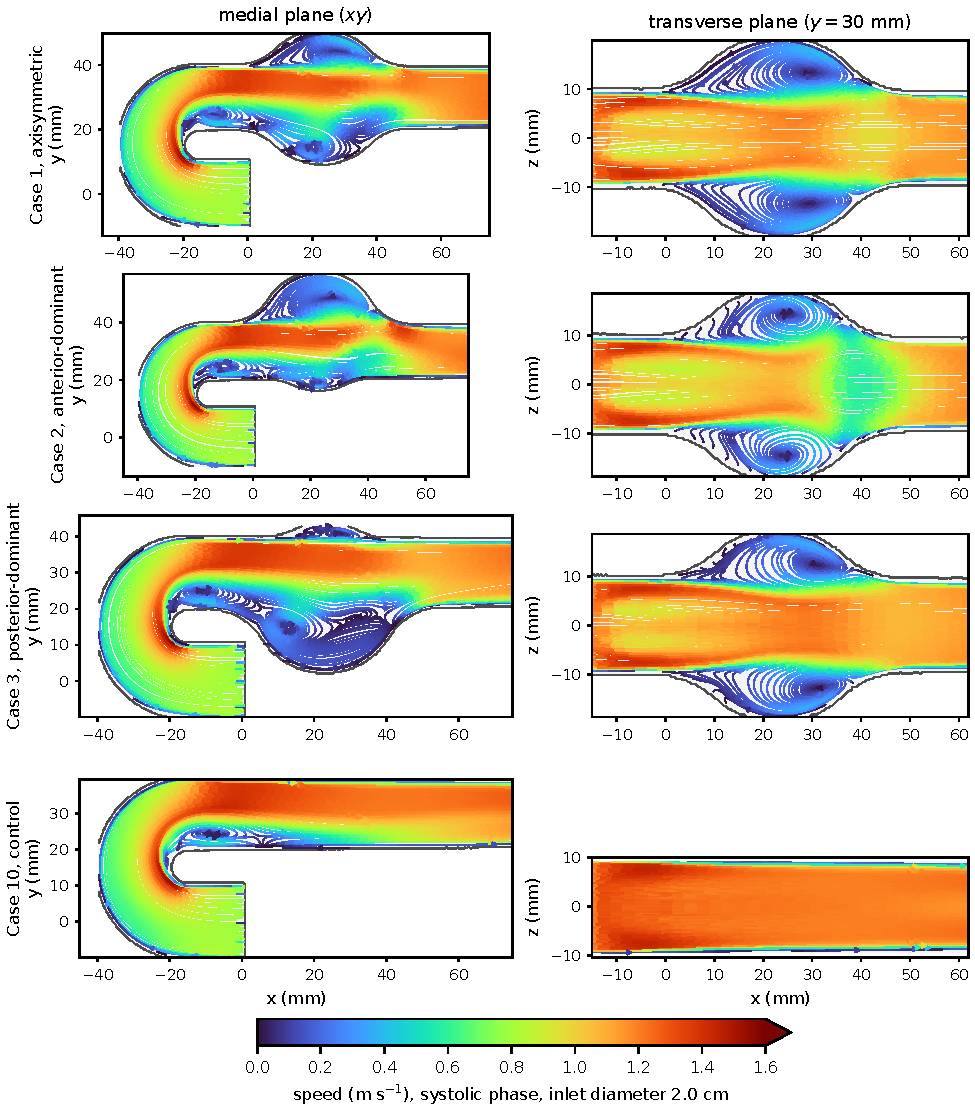
\includegraphics[width=0.92\textwidth]{streamlines_2p0.pdf}
\caption{Streamlines in the systolic phase for the 2.0~cm geometries in the medial plane (left) and the transverse plane (right), colored by in-plane speed on one scale for all geometries. Rows are the axisymmetric, anterior-dominant and posterior-dominant sacs and the control.}
\label{fig:streamlines_2p0}
\end{figure}

\begin{figure}[p]
\centering
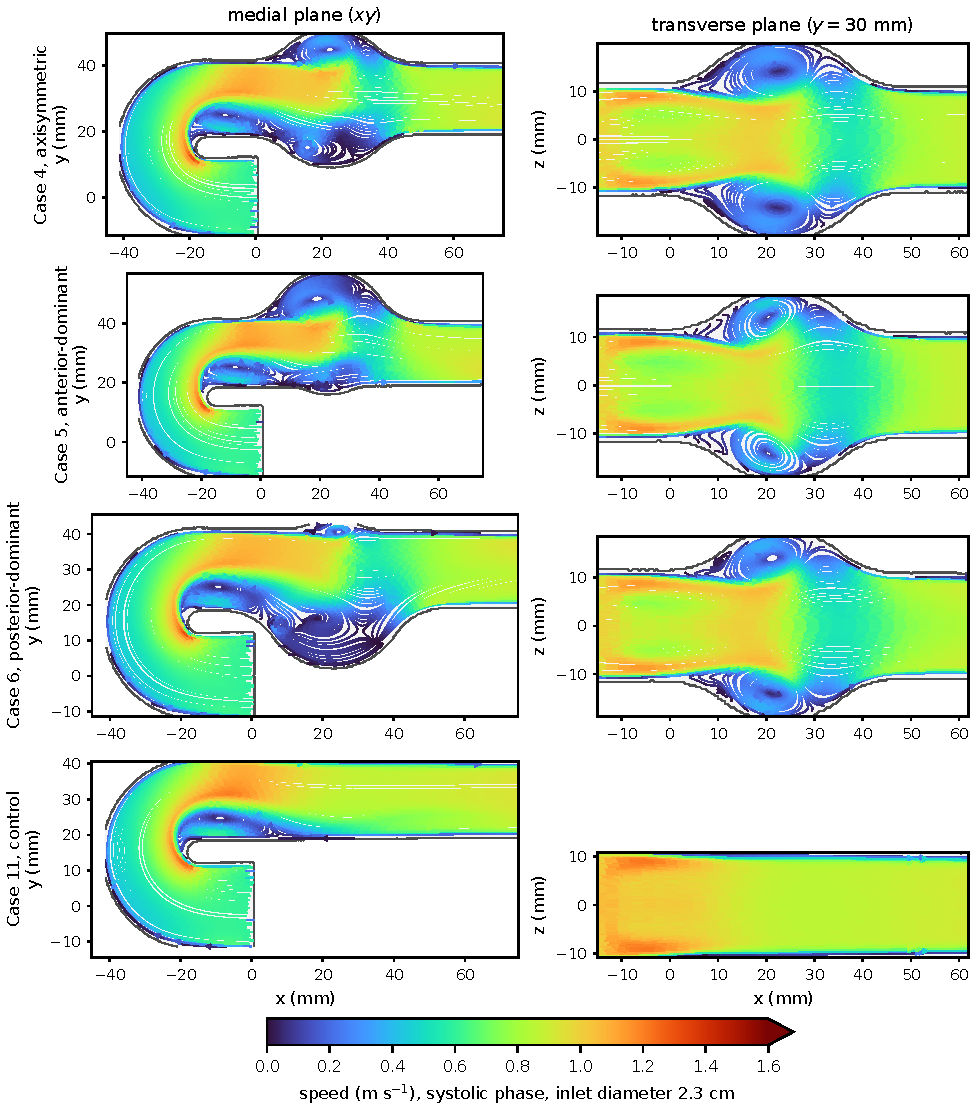
\includegraphics[width=0.92\textwidth]{streamlines_2p3.pdf}
\caption{As Figure~\ref{fig:streamlines_2p0}, for the 2.3~cm geometries.}
\label{fig:streamlines_2p3}
\end{figure}

\begin{figure}[p]
\centering
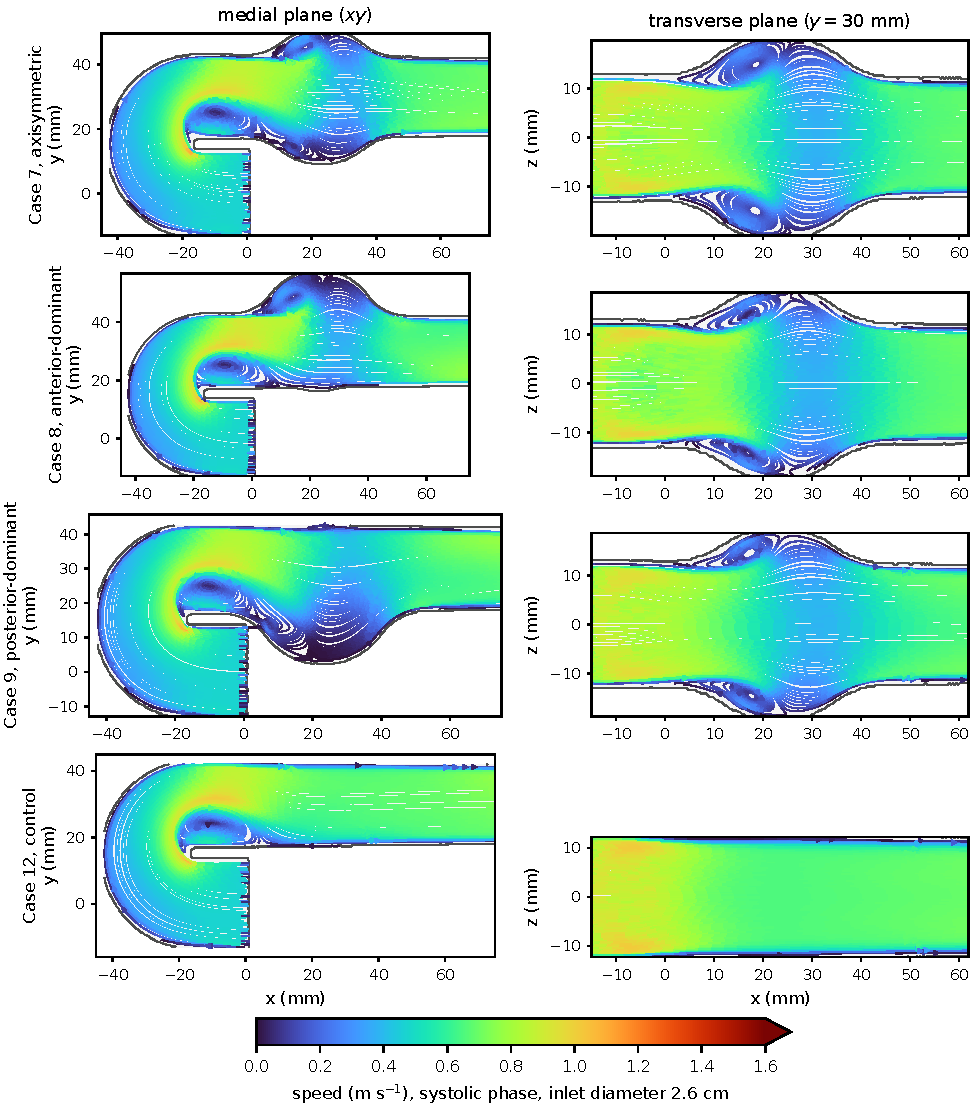
\includegraphics[width=0.92\textwidth]{streamlines_2p6.pdf}
\caption{As Figure~\ref{fig:streamlines_2p0}, for the 2.6~cm geometries.}
\label{fig:streamlines_2p6}
\end{figure}


\subsection{Pressure drop, reversed flow and eddy viscosity}
Table~\ref{tab:cfd_summary} summarizes the common-time flow descriptors for all twelve geometries, and inlet diameter clearly dominates the systolic response. The inlet-to-outlet pressure drop in the systolic phase decreases from \(1261\)--\(1346\,\mathrm{Pa}\) at \(2.0\,\mathrm{cm}\) to \(844\)--\(870\,\mathrm{Pa}\) at \(2.3\,\mathrm{cm}\) and \(528\)--\(561\,\mathrm{Pa}\) at \(2.6\,\mathrm{cm}\), whereas at a fixed diameter the three bulge patterns differ by at most \(7\%\). Relative to the matched control, the dilation adds \(17\)--\(30\%\) to the pressure drop. The fraction of dilation-segment nodes exhibiting reversed axial velocity at systole follows the same ordering, falling from \(50\)--\(54\%\) at \(2.0\,\mathrm{cm}\) to \(38\)--\(40\%\) at \(2.3\,\mathrm{cm}\) and \(24\)--\(28\%\) at \(2.6\,\mathrm{cm}\), against only \(2\)--\(3\%\) in the controls. The mean eddy viscosity within the segment is \(8.6\)--\(9.5\) times the molecular viscosity at \(2.0\,\mathrm{cm}\) but only \(1.6\)--\(2.1\) times at \(2.6\,\mathrm{cm}\). A narrower parent vessel therefore delivers a faster jet into the same \(4.0\,\mathrm{cm}\) sac, producing a larger expansion, a greater fraction of reversed flow, and stronger modeled turbulent mixing. At diastole, by contrast, the pressure drops are only \(1.6\)--\(10.7\,\mathrm{Pa}\), and \(35\)--\(47\%\) of the segment carries reversed flow in every geometry, including the controls, because the slow plateau flow no longer possesses a coherent core.

% Generated by generate_cfd_summary.py from data/processed/full (rigid-wall CFD); CSV: report/tables/eacfm_cfd_summary.csv
\begin{table}[htbp]
\centering
\small
\setlength{\tabcolsep}{3.2pt}
\caption{Common-time descriptors of the rigid-wall \CFD at systole (1.780~s) and
diastole (2.400~s). $\Delta p$ is the difference between the mean static pressure
on the inlet and outlet faces, and the reversed-flow fraction is the fraction of
nodes with $u_x<0$, the local downstream direction in the straight segment. The
evaluation segment is the dilation segment of Section~\ref{sec:exports}; all values
are node-weighted descriptive summaries of single designed geometries.}
\label{tab:cfd_summary}
\resizebox{\textwidth}{!}{%
\begin{tabular}{ccc rr cc cc c cc c}
\toprule
 & & & \multicolumn{2}{c}{$\Delta p$ (Pa)} & \multicolumn{2}{c}{Systolic $\tau_w$ (Pa)} & \multicolumn{2}{c}{Diastolic $\tau_w$ (Pa)} & Mean speed & \multicolumn{2}{c}{Reversed flow (\%)} & $\overline{\mu_t}/\mu$ \\
\cmidrule(lr){4-5}\cmidrule(lr){6-7}\cmidrule(lr){8-9}\cmidrule(lr){11-12}
Case & $D_{\rm in}$ (cm) & $\beta$ & Sys. & Dia. & Median & 95th pct. & Median & 95th pct. & sys. (m~s$^{-1}$) & Sys. & Dia. & sys. \\
\midrule
1 & 2.0 & 1.00 & 1261 & 10.7 & 1.94 & 17.6 & 0.279 & 0.60 & 0.362 & 50 & 35 & 9.5 \\
2 & 2.0 & 0.48 & 1346 & 3.1 & 2.83 & 17.4 & 0.729 & 1.07 & 0.391 & 50 & 45 & 9.4 \\
3 & 2.0 & 2.08 & 1297 & 5.7 & 1.65 & 15.4 & 0.851 & 1.24 & 0.346 & 54 & 45 & 8.6 \\
4 & 2.3 & 1.00 & 844 & 6.8 & 2.30 & 11.7 & 0.253 & 0.46 & 0.328 & 39 & 37 & 3.6 \\
5 & 2.3 & 0.48 & 870 & 1.7 & 2.39 & 10.7 & 0.613 & 0.98 & 0.330 & 38 & 46 & 4.0 \\
6 & 2.3 & 2.08 & 870 & 7.0 & 2.06 & 10.8 & 0.486 & 0.89 & 0.316 & 40 & 43 & 3.2 \\
7 & 2.6 & 1.00 & 545 & 4.9 & 1.87 & 8.1 & 0.251 & 0.59 & 0.275 & 28 & 38 & 1.6 \\
8 & 2.6 & 0.48 & 561 & 1.6 & 1.85 & 7.4 & 0.515 & 0.83 & 0.274 & 28 & 46 & 2.0 \\
9 & 2.6 & 2.08 & 528 & 5.8 & 1.82 & 7.1 & 0.447 & 0.91 & 0.261 & 24 & 47 & 2.1 \\
10 & 2.0 & Control & 1074 & 6.6 & 5.02 & 8.8 & 0.125 & 0.52 & 0.730 & 2 & 35 & 4.2 \\
11 & 2.3 & Control & 668 & 2.8 & 3.53 & 4.9 & 0.103 & 0.38 & 0.546 & 3 & 41 & 2.6 \\
12 & 2.6 & Control & 448 & 1.7 & 2.65 & 3.5 & 0.172 & 0.30 & 0.434 & 3 & 43 & 2.0 \\
\bottomrule
\end{tabular}%
}
\end{table}


\subsection{Wall shear stress}
Figure~\ref{fig:wss_sys} illustrates the \WSS magnitude over the dilation segment in the systolic phase, unwrapped about the axis of the descending segment. In this representation the anterior wall lies at \(0^\circ\) and the posterior wall at \(\pm180^\circ\), so that the full circumference of the vessel is displayed on a single plane. At systole all aneurysmal cases share a low-shear sac body bounded by high-shear rings at the proximal and distal necks, where the jet enters the sac and reattaches. The median segment \WSS is 1.6--2.8~Pa in the aneurysmal cases against 2.7--5.0~Pa in the controls, whereas the 95th percentile is 1.8--2.4 times that of the matched control (Table~\ref{tab:cfd_summary}). The neck rings weaken with increasing inlet diameter, and the 95th percentile falls from 15--18~Pa at 2.0~cm to 7--8~Pa at 2.6~cm. Asymmetry moves the pattern rather than scaling it. In the anterior-dominant cases the low-shear region is centered on the anterior wall (\(0^\circ\)), whereas in the posterior-dominant cases it is centered on the posterior wall (\(\pm180^\circ\)), so that over the sac body the wall opposite the dominant bulge carries the higher shear. In Case~2 the median sac-body \WSS is 4.5~Pa on the posterior wall against 0.9~Pa on the anterior bulge, and in Case~3 the 95th percentile is 8.4~Pa on the anterior wall against 2.1~Pa on the posterior bulge, with the same ordering in Cases~5, 6 and 9 and nearly equal values in Case~8. This behavior is consistent with the streamlines, which show that the jet crossing the sac impinges on the wall opposite the bulge while the bulge itself is filled by slow recirculating flow. At the distal neck the highest shear lies on the anterior (outer-curvature) side in most cases, irrespective of the bulge direction, because the core leaves the bend along the anterior wall.

Figure~\ref{fig:wss_dia} presents the same \WSS magnitude in the diastolic phase on one color scale per phase. At diastole the effect of asymmetry becomes larger than that of diameter. The median segment \WSS of the asymmetric sacs is 0.45--0.85~Pa, which is 1.8--3.1 times that of the axisymmetric sacs (0.25--0.28~Pa) at every diameter and 2.6--6.8 times that of the controls (0.10--0.17~Pa). On comparison of all cases, the diastolic maps show broad shear over the whole wall of the asymmetric sacs, consistent with a residual vortex that keeps moving along the sac wall during the plateau, whereas the axisymmetric sacs and the controls are close to stagnant. These are instantaneous values at two instants; the cycle-averaged picture is given by the \TAWSS maps in Section~\ref{sec:tawss}.

\begin{figure}[!htb]
\centering
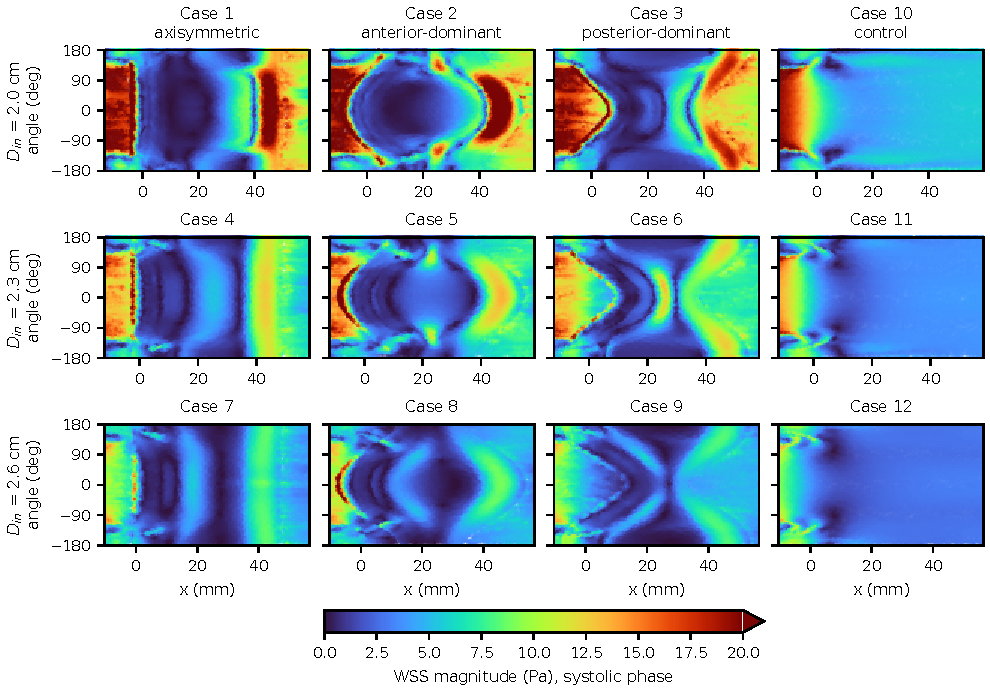
\includegraphics[width=\textwidth]{wss_montage_systole.pdf}
\caption{\WSS magnitude on the dilation segment in the systolic phase, on one color scale saturating at 20~Pa. The wall is unwrapped about the vessel axis, with the anterior wall at \(0^\circ\) and the posterior wall at \(\pm180^\circ\). Rows are inlet diameters and the last column is the matching control. White points are gaps in the exported wall nodes.}
\label{fig:wss_sys}
\end{figure}

\begin{figure}[!htb]
\centering
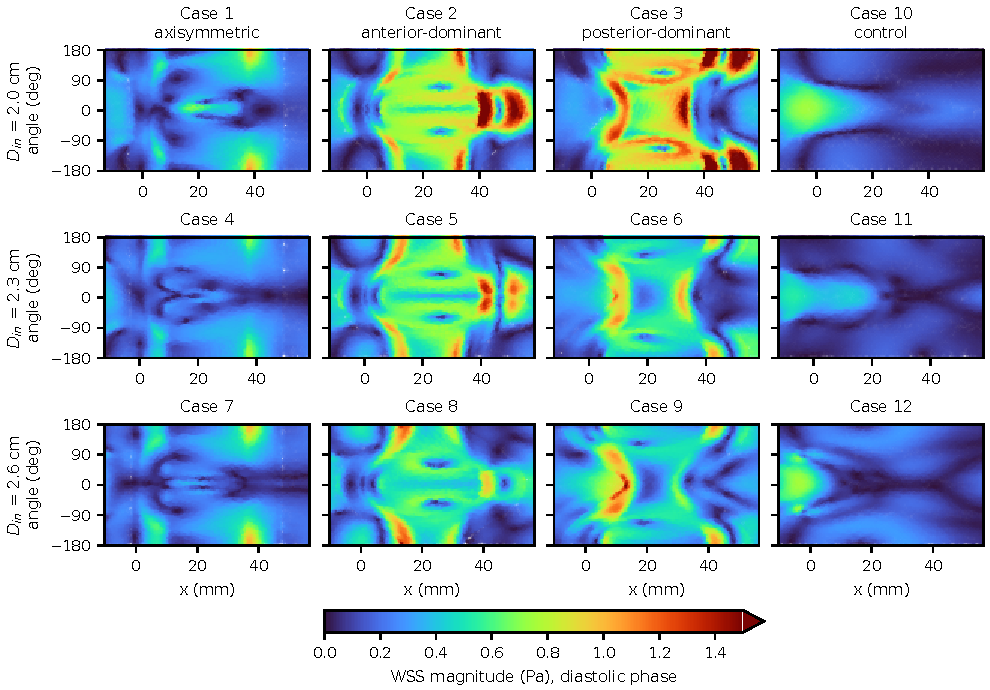
\includegraphics[width=\textwidth]{wss_montage_diastole.pdf}
\caption{As Figure~\ref{fig:wss_sys}, in the diastolic phase, with one color scale saturating at 1.5~Pa.}
\label{fig:wss_dia}
\end{figure}

Figure~\ref{fig:xwss} illustrates the 2D graphics of \WSS for both the medial and transverse planes. Figure~\ref{fig:xwss}(a) represents the \WSS on the anterior wall of the medial plane while Figure~\ref{fig:xwss}(b) shows the \WSS on the posterior wall of the medial plane. Figure~\ref{fig:xwss}(c) presents the \WSS for the transverse plane. Because the aorta bends, a negative value alone does not prove local reverse flow in the curved segment, but along the straight descending segment the negative regions coincide with the recirculation seen in Figures~\ref{fig:streamlines_2p0}--\ref{fig:streamlines_2p6}. On the anterior medial wall and on the transverse wall, \WSS is large and positive at the proximal neck in every case. It becomes negative where the flow detaches on entering the sac, between \(x\approx-4\) and 16~mm on the anterior wall and between 0 and 4~mm on the transverse wall, and it stays negative over the recirculating part of the sac. It returns to positive values, marking reattachment of the core flow, between \(x\approx27\) and 42~mm on the anterior wall and between 26 and 39~mm on the transverse wall, followed by the high positive values of the distal neck. The reattachment point moves upstream as the inlet diameter increases, from 34--42~mm at 2.0~cm to 27--31~mm at 2.6~cm on the anterior wall and from 36--39~mm to 26--27~mm on the transverse wall, so the recirculation region shortens with a wider parent vessel, in line with the reversed-flow fractions of Table~\ref{tab:cfd_summary}. The posterior medial wall differs because \WSS is already negative at the proximal neck in every geometry, the controls included, which identifies this region as the \ICRZ rather than as part of the sac recirculation. The depth of the negative region does not follow the bulge pattern consistently; the most negative value inside the sac, \(-11.3\)~Pa, occurs on the anterior wall of Case~6.

\begin{figure}[!htb]
\centering
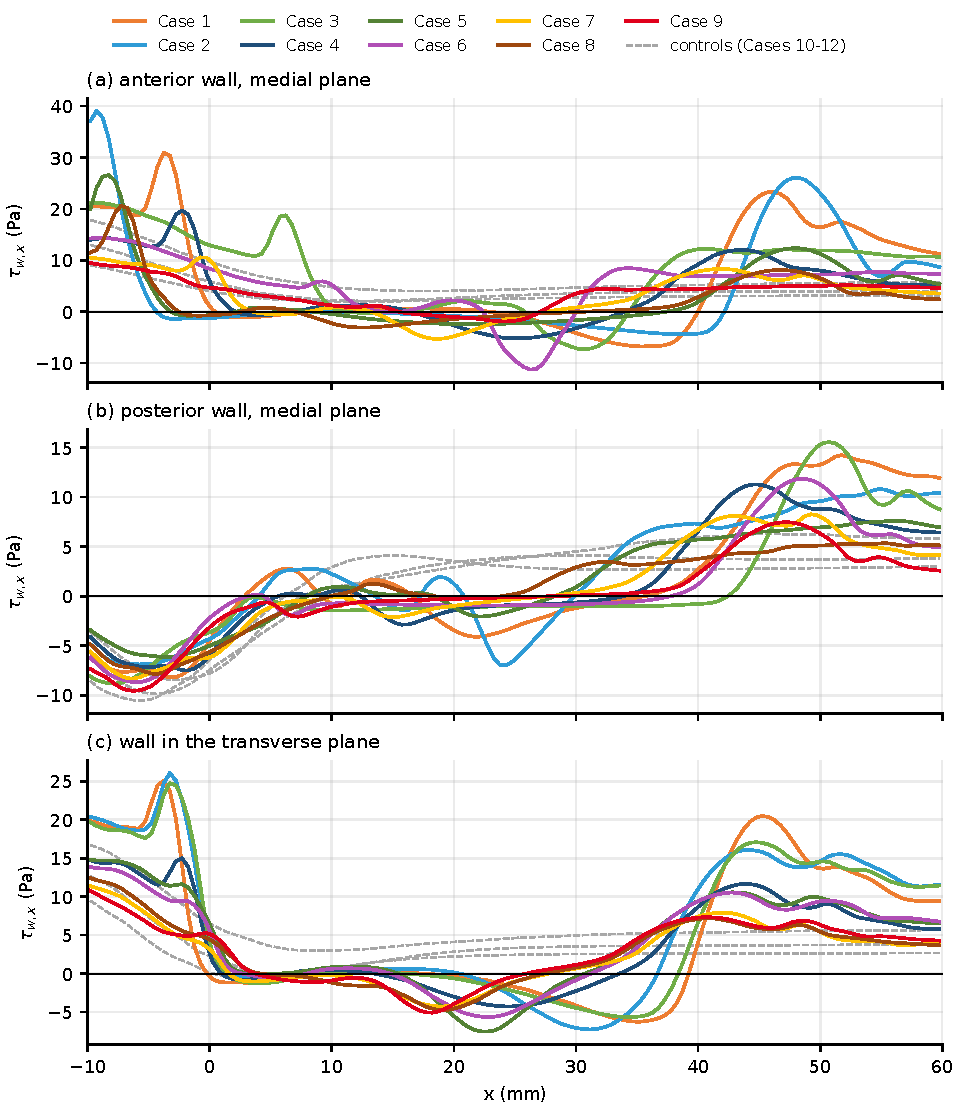
\includegraphics[width=0.85\textwidth]{xwss_lines.pdf}
\caption{2D graphics of \WSS (Pa) in the medial and transverse planes at systolic phase: (a) anterior side of the medial plane, (b) posterior side of the medial plane, and (c) transverse plane.}
\label{fig:xwss}
\end{figure}

\subsection{Time-averaged wall shear stress}
\label{sec:tawss}

The analysis of \TAWSS, as presented in Figure~\ref{fig:tawss} and Table~\ref{tab:tawss}, across twelve idealized geometries revealed several consistent trends. The \TAWSS is shown on the dilation segment of every geometry, unwrapped as in Figure~\ref{fig:wss_sys} and drawn on one logarithmic color scale because the values span two orders of magnitude. Every aneurysmal sac carries a broad region of low \TAWSS. The median over the dilation segment is 0.51--0.83~Pa in the aneurysmal cases against 2.5--4.5~Pa over the same stretch of the controls, while over the sac body the median on either side is 0.23--0.84~Pa. Relative to the matched control, the segment median is lower by a factor of 8.5--8.9 at 2.0~cm, 4.0--4.9 at 2.3~cm and 3.4--3.6 at 2.6~cm, so that the reduction in cycle-averaged shear caused by the dilation is largest for the narrowest parent vessel. Increasing the inlet diameter from 2~cm to 2.6~cm was associated with a progressive reduction in \TAWSS. The high-shear rings at the necks persist in the cycle average, and their strength falls with inlet diameter, the 95th percentile decreasing from 7.6--10.9~Pa at 2.0~cm to 5.5--6.4~Pa at 2.3~cm and 4.1--5.1~Pa at 2.6~cm.

Aneurysm asymmetry had a strong influence on the spatial distribution of \TAWSS. In asymmetric models, the lowest \TAWSS is consistently placed on the dominant bulge. In the anterior-dominant Cases~2, 5 and 8 the sac-body median is 0.34, 0.23 and 0.33~Pa on the anterior wall against 0.52, 0.58 and 0.84~Pa on the posterior wall, whereas in the posterior-dominant Cases~6 and 9 it is 0.24 and 0.28~Pa on the posterior wall against 0.71 and 0.60~Pa on the anterior wall. Case~3 is the exception, with similar values on both sides (0.35 and 0.42~Pa). In the axisymmetric sacs the low-shear region forms circumferential bands with nearly equal anterior and posterior medians. It is also observed that the bulge side is where the instantaneous shear is lowest at systole, so that the dominant bulge is exposed to low shear over the whole cycle rather than at a single instant. This reinforces the need for a multi-parametric hemodynamic assessment that includes both \WSS and \TAWSS to identify rupture-prone \DTAAs. Low \TAWSS, in particular, marks regions of prolonged low shear, which are known to promote thrombus formation~\cite{salman2019biomechanical}, although the present models do not include those processes.

\begin{figure}[!htb]
\centering
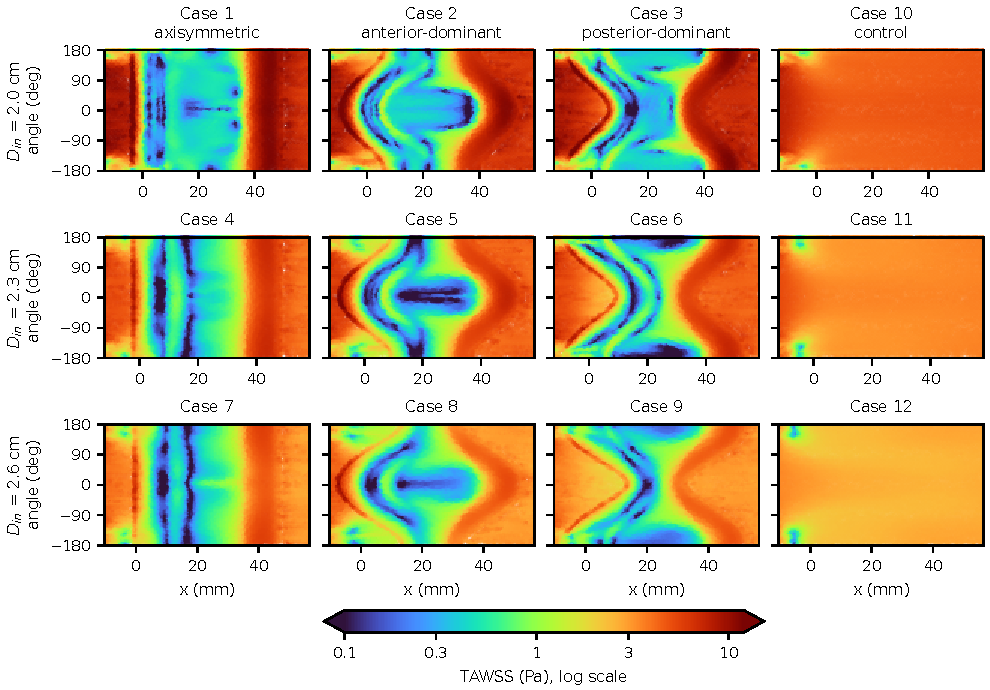
\includegraphics[width=\textwidth]{tawss_montage.pdf}
\caption{\TAWSScap on the dilation segment, unwrapped as in Figure~\ref{fig:wss_sys}, on one logarithmic color scale. Rows are inlet diameters and the last column is the matching control.}
\label{fig:tawss}
\end{figure}

% Generated by scripts/manuscript/generate_wss_montage.py from data/raw/TAWSS 30.09.2026.
\begin{table}[htbp]
\centering
\small
\caption{\revision{TAWSS (Pa) on the dilation segment. Percentiles are over the whole segment, while the sac-body medians use its middle third, within $60^\circ$ of the anterior or posterior direction.}}
\label{tab:tawss}
\begin{tabular}{cclccccc}
\toprule
 & & & \multicolumn{3}{c}{Segment} & \multicolumn{2}{c}{Sac body, median} \\
\cmidrule(lr){4-6}\cmidrule(lr){7-8}
Case & $D_{\rm in}$ (cm) & Morphology & 5th pct. & Median & 95th pct. & Anterior & Posterior \\
\midrule
1 & 2.0 & axisymmetric & 0.19 & 0.51 & 10.86 & 0.41 & 0.47 \\
2 & 2.0 & anterior-dominant & 0.15 & 0.52 & 7.60 & 0.34 & 0.52 \\
3 & 2.0 & posterior-dominant & 0.18 & 0.53 & 8.66 & 0.35 & 0.42 \\
10 & 2.0 & control & 3.65 & 4.53 & 4.89 & 4.66 & 4.36 \\
4 & 2.3 & axisymmetric & 0.12 & 0.70 & 6.41 & 0.47 & 0.49 \\
5 & 2.3 & anterior-dominant & 0.10 & 0.67 & 5.45 & 0.23 & 0.58 \\
6 & 2.3 & posterior-dominant & 0.10 & 0.83 & 5.82 & 0.71 & 0.24 \\
11 & 2.3 & control & 2.81 & 3.30 & 3.52 & 3.45 & 3.20 \\
7 & 2.6 & axisymmetric & 0.12 & 0.70 & 5.06 & 0.45 & 0.50 \\
8 & 2.6 & anterior-dominant & 0.17 & 0.73 & 4.12 & 0.33 & 0.84 \\
9 & 2.6 & posterior-dominant & 0.18 & 0.69 & 4.24 & 0.60 & 0.28 \\
12 & 2.6 & control & 2.20 & 2.51 & 2.82 & 2.59 & 2.51 \\
\bottomrule
\end{tabular}
\end{table}


\FloatBarrier

\subsection{Structural wall stress}
\label{sec:structural}

It is widely recognized that aneurysm rupture risk is associated with maximum diameter; however, this relationship is not absolute. Darling et al.~\cite{darling1977autopsy} observed that some large aneurysms do not rupture, whereas smaller ones do, indicating that additional factors such as aneurysm geometry and asymmetry play a critical role. Aneurysm rupture occurs when the mechanical load exceeds the tissue strength of the arterial wall, and understanding this mechanical mechanism is essential for assessing rupture risk in \DTAA. Our results indicate that aneurysm shape and inlet diameter markedly change the modeled wall-stress distribution. Previous studies, including those by Dobrin~\cite{dobrin1989pathophysiology}, have applied Laplace's law to estimate wall stress. However, Laplace's law predicts the greatest wall stress at the maximum bulge of the aneurysm sac, which is not consistent with the biomechanical behavior observed in aneurysmal geometries. As demonstrated in the present study, the stress distribution within the aneurysm wall is governed by asymmetry and geometric features.

Figure~\ref{fig:mps} presents the \MPS on the inner surface of the wall over the dilation segment, unwrapped as in Figure~\ref{fig:wss_sys}, and Table~\ref{tab:mps} summarizes it. In every aneurysmal case the \MPS is highest in circumferential bands at the necks, where the wall curvature changes sign, with 95th percentiles of 101--113~kPa over the necks, and lowest over the crown of the sac, where the medians are 55--80~kPa. This pattern is consistent with the findings of Vorp et al.~\cite{vorp1998mechanical}. A clear distinction was observed between axisymmetric and asymmetric cases. In the axisymmetric models, the stress was elevated at the proximal regions but lower at the midsection of the aneurysm sac, with similar behavior on both anterior and posterior sides; the anterior and posterior sac-body medians are equal to within 1~kPa. In contrast, the asymmetric models exhibited higher stress on the side opposite to the dominant bulge. The sac-body median on the posterior wall of the anterior-dominant Cases~2, 5 and 8 is 69.2, 73.6 and 78.1~kPa against 55.9, 55.0 and 61.8~kPa on the anterior bulge, and the anterior wall of the posterior-dominant Cases~3, 6 and 9 carries 68.3, 72.9 and 80.3~kPa against 55.8, 55.3 and 57.2~kPa on the posterior bulge. The opposite-side value increases with inlet diameter, as does the segment median of the controls (52.5, 58.4 and 65.1~kPa), because the loaded radius grows with the parent vessel.

In contrast, the healthy cases (10--12) exhibited relatively uniform wall stress distributions, with 95th percentiles within 3~kPa of their medians and only mild elevations at the bend. Compared to the diseased cases, where stress varied non-uniformly due to the presence of the aneurysm, the healthy aortas showed more consistent stress profiles. Assuming uniform wall strength, these results indicate that the side opposite to the dominant bulge is at a higher risk of rupture compared to the other side. Among the six asymmetric cases, the highest \MPS was observed in Case~9 on the anterior side, so that, if the wall strength were the same on both sides, this site would carry the highest modeled stress of all sides and cases. With a uniform 2~mm wall, literature material parameters, fixed ends and a quasi-static coupling whose step settings were not retained, the stress magnitudes indicate where the modeled wall is most loaded rather than where it would fail, since failure also depends on the unknown local wall strength.

\begin{figure}[!htb]
\centering
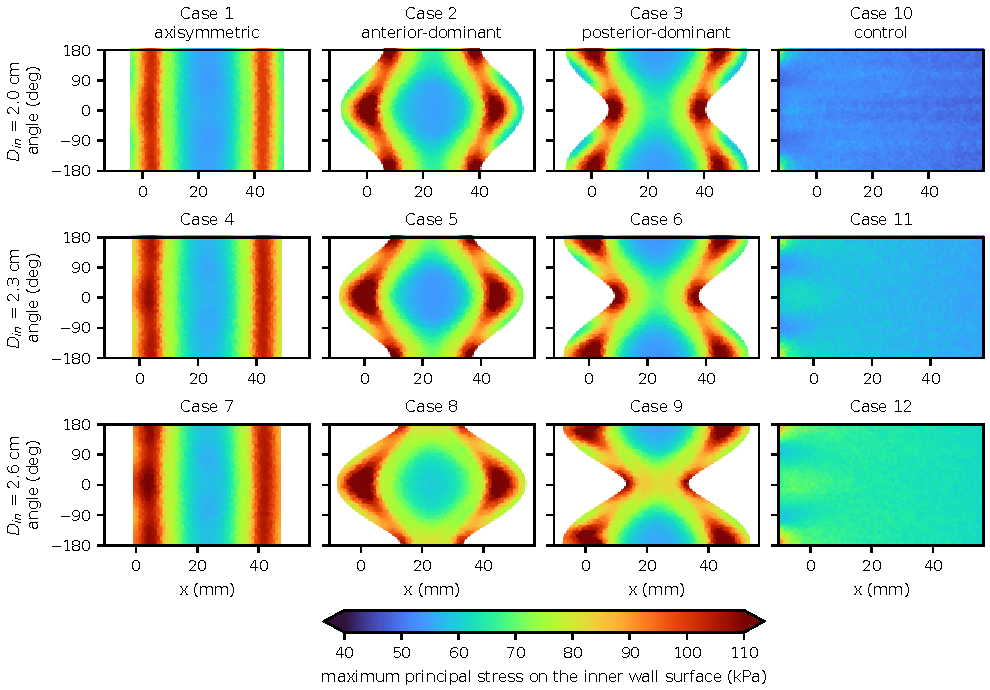
\includegraphics[width=\textwidth]{mps_montage.pdf}
\caption{\MPScap on the inner wall surface of the dilation segment, unwrapped as in Figure~\ref{fig:wss_sys}, on one color scale. Rows are inlet diameters and the last column is the matching control.}
\label{fig:mps}
\end{figure}

% Recomputed 2026-10-16 from data/raw/MPS; Case 8 uses the replacement data/Case 8.xls.
\begin{table}[htbp]
\centering
\small
\caption{\revision{Maximum principal stress (kPa) on the inner wall surface of the dilation segment. Sac-body medians use the middle third of the segment, within $60^\circ$ of the anterior or posterior direction, while the neck value is the 95th percentile over the outer thirds.}}
\label{tab:mps}
\begin{tabular}{cclccccc}
\toprule
 & & & \multicolumn{2}{c}{Segment} & \multicolumn{2}{c}{Sac body, median} & Necks \\
\cmidrule(lr){4-5}\cmidrule(lr){6-7}\cmidrule(lr){8-8}
Case & $D_{\rm in}$ (cm) & Morphology & Median & 95th pct. & Anterior & Posterior & 95th pct. \\
\midrule
1 & 2.0 & axisymmetric & 67.6 & 99.5 & 56.7 & 56.7 & 101.0 \\
2 & 2.0 & anterior-dominant & 70.2 & 106.9 & 55.9 & 69.2 & 111.3 \\
3 & 2.0 & posterior-dominant & 69.8 & 105.5 & 68.3 & 55.8 & 110.0 \\
10 & 2.0 & control & 52.5 & 54.8 & 52.4 & 52.8 & 54.9 \\
4 & 2.3 & axisymmetric & 71.4 & 103.9 & 58.1 & 59.0 & 104.5 \\
5 & 2.3 & anterior-dominant & 72.4 & 108.5 & 55.0 & 73.6 & 113.4 \\
6 & 2.3 & posterior-dominant & 72.2 & 107.4 & 72.9 & 55.3 & 112.1 \\
11 & 2.3 & control & 58.4 & 60.7 & 58.7 & 58.9 & 61.0 \\
7 & 2.6 & axisymmetric & 74.1 & 105.2 & 59.4 & 60.6 & 106.3 \\
8 & 2.6 & anterior-dominant & 75.9 & 111.6 & 55.3 & 80.5 & 117.7 \\
9 & 2.6 & posterior-dominant & 76.5 & 107.3 & 80.3 & 57.2 & 112.9 \\
12 & 2.6 & control & 65.1 & 67.6 & 65.3 & 65.7 & 68.0 \\
\bottomrule
\end{tabular}
\end{table}


\FloatBarrier

\subsection{Plane-wise flow summaries}
\label{sec:planes}

In addition to the wall-based hemodynamic and biomechanical indices, a plane-wise cross-sectional analysis was performed to quantify the spatial variation of flow features along the aorta. Velocity and \TKE were evaluated at selected axial planes to identify the regions where aneurysm morphology most strongly altered the flow field. This approach allows the three-dimensional flow disturbance to be reduced into comparable regional quantities from the proximal to distal sections of the vessel.

The locations of the eight planes are shown in Figure~\ref{fig:diagram} and the details of aortic diameter are available in Table~\ref{tab:diameter}. All models incorporated a taper ratio of 0.8 from inlet to outlet, a physiologically important feature that gradually reduces the vessel diameter distally, thereby maintaining flow momentum and regulating perfusion to downstream vessels. Figure~\ref{fig:planes} shows the plane-averaged speed and \TKE of every case from the retained slice summaries, and Table~\ref{tab:plane_cfd} gives the medians of the aneurysmal and control groups. The taper is visible in every model, with the speed at D7 and D8 above that at D1--D3 because the lumen narrows toward the outlet. This tapering-induced acceleration is essential for maintaining adequate perfusion pressure that ensures sufficient blood flow to downstream vascular beds. Indeed, studies have shown that flow velocity increases while vessel diameter decreases~\cite{kahveci2015numerical}. In the aneurysmal cases the speed falls sharply across the sac to 0.10--0.16~m~s$^{-1}$ at D5, where the lumen diameter is 4.0~cm whatever the inlet diameter, against a median of 0.193~m~s$^{-1}$ in the controls, and it recovers by D7. This is a direct consequence of the local dilation, where the increased cross-sectional area reduces flow velocity to conserve mass.

In contrast to velocity, the modeled $k$ as shown in Figure~\ref{fig:planes} rises through the sac, peaks at D5 at about twice the control value, remains elevated at D6 and D7, where the jet reattaches and the recirculation of the distal sac develops, and returns to the control level by D8. At plane~5 (the maximum diameter of the bulge, the center of the aneurysm sac), strong flow separation and recirculation zones produce high $k$. At plane~6 (distal sac) and plane~7 (post-aneurysm), $k$ remains elevated, implying that the disturbed flow persists downstream of the aneurysm sac. This pattern is consistent with the fact that recirculation zones predominantly appear on the distal side of the aneurysm, where the flow jet impinges and vortices develop~\cite{yu2000steady}. Conversely, at D4, the proximal neck, the aneurysmal and control values still overlap, so the turbulent disturbance is generated inside the sac rather than at its entrance, and it decays within about one sac length downstream. Thus, $k$ only rises sharply once the flow reaches the central and distal portions of the sac, where recirculation becomes fully established. By plane~8 (near the outlet), the $k$ has returned to the control level, demonstrating that the turbulence has largely dissipated before reaching the distal boundary. The asymmetric sacs reach higher $k$ at D5 than the axisymmetric ones at every diameter.

Overall, the plane-wise analysis confirms that the aneurysm-induced flow disturbance is highly localized rather than uniformly distributed along the entire aorta. The velocity results identified the strongest reduction at plane~5, corresponding to the maximum aneurysm diameter, whereas the $k$ results showed that disturbed and vortical flow persists from the aneurysm center to the distal sac and post-aneurysm region. Thus, the plane-based quantities provide complementary information to the wall-based indices. While \WSS and \TAWSS describe near-wall hemodynamic loading and \MPS describes structural wall stress, the plane-wise velocity and $k$ analysis captures the intraluminal flow disturbance and its downstream propagation. Therefore, the plane-wise analysis provides quantitative evidence that the maximum aneurysm diameter primarily reduces local velocity, whereas aneurysm morphology and sac expansion generate elevated \TKE over a broader downstream region.

\begin{figure}[!htb]
\centering
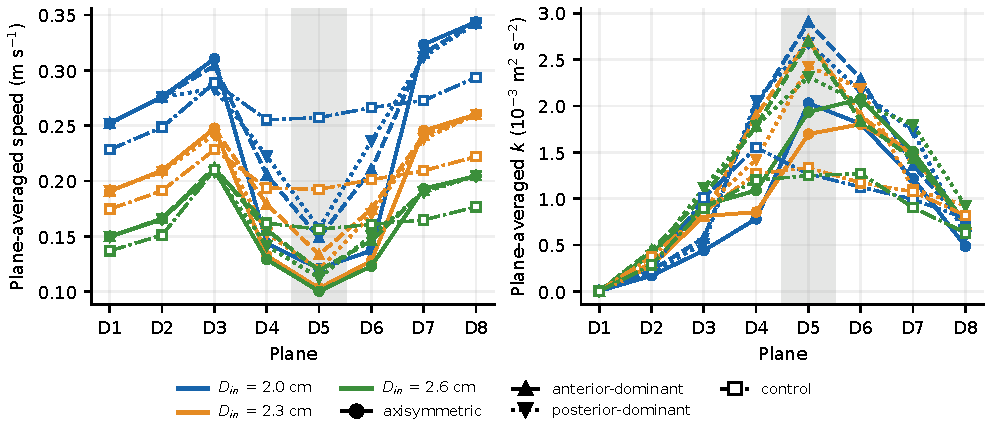
\includegraphics[width=\textwidth]{plane_profiles.pdf}
\caption{Plane-averaged speed (left) and \TKE per unit mass (right) at D1--D8 for all twelve geometries. Color gives the inlet diameter, and line style and marker the morphology; controls are dash-dot with open squares. The band marks the sac center (D5).}
\label{fig:planes}
\end{figure}

% Generated from corrected data/results_on_slices.csv on 2026-09-27.
\begin{table}[htbp]
\centering
\caption{Descriptive medians of the reported plane-averaged CFD quantities across nine aneurysmal and three control geometries. $k$ is turbulent kinetic energy per unit mass (m$^2$~s$^{-2}$). These designed cases do not support patient-population significance tests.}
\label{tab:plane_cfd}
\begin{tabular}{lcccc}
\toprule
& \multicolumn{2}{c}{Mean speed (m~s$^{-1}$)} & \multicolumn{2}{c}{$k$ ($10^{-3}$ m$^2$~s$^{-2}$)} \\
Plane & Aneurysmal & Control & Aneurysmal & Control \\
\midrule
D1 & 0.191 & 0.175 & 0.002 & 0.003 \\
D2 & 0.209 & 0.191 & 0.275 & 0.287 \\
D3 & 0.247 & 0.228 & 0.815 & 0.896 \\
D4 & 0.153 & 0.194 & 1.783 & 1.270 \\
D5 & 0.120 & 0.193 & 2.425 & 1.266 \\
D6 & 0.151 & 0.201 & 2.028 & 1.171 \\
D7 & 0.241 & 0.209 & 1.468 & 0.993 \\
D8 & 0.260 & 0.222 & 0.728 & 0.788 \\
\bottomrule
\end{tabular}
\end{table}


\section{Reconstruction results}
\label{sec:reconstruction_results}
\subsection{Checks on the complete \texorpdfstring{\CFD}{CFD} fields}
\label{sec:reference_results}
Before any fitting, the complete \CFD fields of the nine aneurysmal cases were used to check Eq.~\eqref{eq:momentum} and to measure the post-processing floors. With 40-neighbor least-squares gradients, the unsteady form with the \CFD eddy viscosity and without a $2\rho k/3$ term gave the smallest momentum residual in every case and phase, at 0.03--0.17 of the convective term in the bulk of the lumen. Omitting the time derivative raised the residual to 0.18--0.30 of convection at systole, and to 0.45--0.56 inside the sac, and to 0.49--0.73 at diastole, and adding the $2\rho k/3$ term made the residual larger. A quasi-steady momentum residual is therefore not consistent with these transient fields, particularly inside the sac.

Table~\ref{tab:reference_floor} gives the floors obtained by passing the complete \CFD velocity through the shared post-processing. Integrating the \CFD's own pressure gradient reproduces the \CFD pressure to 0.5--0.9\%, so the integration itself is accurate, and the remaining floor comes from the momentum terms. With the unsteady form and oracle $\mu_t$ the pressure floor is 1.6--2.3\% at systole, except for Case~2, whose forward window gives 7.1\%, and 2.2--4.1\% at diastole. Information matters differently in the two phases. At systole the molecular form is almost as good as the oracle for the 2.3 and 2.6~cm cases (1.8--2.7\%) but not for the 2.0~cm cases (4.9--11.3\%), in line with their larger eddy viscosity (Table~\ref{tab:cfd_summary}). At diastole removing either the time term or the eddy viscosity degrades the floor substantially, to 3.9--10.3\% and 9.0--19.3\%, respectively. The \WSS floor depends strongly on the distance $h$ in Eq.~\eqref{eq:wss_estimate}. At systole it is 0.07--0.09 at $h=0.1$~mm but 0.14--0.27 at the prespecified $h=0.25$~mm, because the systolic velocity profile is no longer close to quadratic over the $2h=0.5$~mm stencil, whereas at diastole it is 0.04--0.06 at either distance.

% Generated by generate_reference_table.py from the cfd run records.
\begin{table}[htbp]
\centering
\small
\setlength{\tabcolsep}{4pt}
\caption{\revision{\textcolor{red}{Pipeline floor, obtained by passing the complete CFD velocity through the shared post-processing. Pressure columns give the sub-cloud relative L2 error for each information setting, combining retention or omission of the time term with either CFD eddy viscosity or molecular viscosity alone. $\Delta p_{\rm sub}$ is the CFD pressure drop between the inlet and outlet ends of the sub-cloud. Wall-shear columns give the aneurysm-zone magnitude error of the one-sided estimate at $h=0.1$~mm and at the prespecified $h=0.25$~mm. Case 2's systolic window runs forward from the target (1.780--1.788~s), which explains its larger unsteady error.}}}
\label{tab:reference_floor}
\begin{tabular}{llccccrcc}
\toprule
 & & \multicolumn{4}{c}{Pressure relative L2} & & \multicolumn{2}{c}{Wall shear} \\
\cmidrule(lr){3-6}\cmidrule(lr){8-9}
Case & Phase & Unst.+$\mu_t$ & Steady+$\mu_t$ & Unst.+$\mu$ & Steady+$\mu$ & $\Delta p_{\rm sub}$ (Pa) & $h=0.1$ & $h=0.25$ \\
\midrule
1 & Sys. & 0.022 & 0.031 & 0.049 & 0.067 & 986.1 & 0.086 & 0.249 \\
1 & Dia. & 0.035 & 0.074 & 0.152 & 0.188 & 8.8 & 0.044 & 0.042 \\
2 & Sys. & 0.071 & 0.027 & 0.113 & 0.048 & 1063.4 & 0.090 & 0.273 \\
2 & Dia. & 0.037 & 0.056 & 0.145 & 0.154 & 1.1 & 0.048 & 0.042 \\
3 & Sys. & 0.022 & 0.029 & 0.065 & 0.071 & 1010.2 & 0.090 & 0.220 \\
3 & Dia. & 0.024 & 0.039 & 0.091 & 0.101 & 3.7 & 0.048 & 0.046 \\
4 & Sys. & 0.019 & 0.037 & 0.023 & 0.036 & 664.2 & 0.077 & 0.182 \\
4 & Dia. & 0.032 & 0.103 & 0.175 & 0.242 & 5.5 & 0.050 & 0.037 \\
5 & Sys. & 0.019 & 0.036 & 0.027 & 0.036 & 682.4 & 0.094 & 0.208 \\
5 & Dia. & 0.031 & 0.051 & 0.114 & 0.121 & 0.4 & 0.052 & 0.041 \\
6 & Sys. & 0.018 & 0.033 & 0.026 & 0.032 & 685.4 & 0.078 & 0.191 \\
6 & Dia. & 0.041 & 0.068 & 0.193 & 0.211 & 5.8 & 0.054 & 0.042 \\
7 & Sys. & 0.016 & 0.037 & 0.018 & 0.035 & 412.8 & 0.070 & 0.151 \\
7 & Dia. & 0.038 & 0.090 & 0.172 & 0.246 & 4.1 & 0.050 & 0.040 \\
8 & Sys. & 0.023 & 0.048 & 0.018 & 0.042 & 422.4 & 0.090 & 0.183 \\
8 & Dia. & 0.039 & 0.065 & 0.154 & 0.160 & 0.6 & 0.055 & 0.043 \\
9 & Sys. & 0.020 & 0.033 & 0.020 & 0.033 & 397.3 & 0.070 & 0.141 \\
9 & Dia. & 0.022 & 0.045 & 0.090 & 0.096 & 4.8 & 0.060 & 0.048 \\
\bottomrule
\end{tabular}
\end{table}


\subsection{Momentum-constrained \texorpdfstring{\PINNs}{PINNs} on the development geometries}
\label{sec:pilot_results}
In the development cases, every neural field reconstructed the hidden velocity three to four times more accurately than \RBF (relative errors 0.037--0.052 versus 0.13--0.16 at systole) and five times more accurately than linear interpolation. However, the prespecified criterion of the development test failed on both endpoints (Table~\ref{tab:pilot}). The momentum arms were trained with a blood density of 1060~kg~m$^{-3}$ in the scaling of their residual before the density was corrected to 1050~kg~m$^{-3}$; all reported scores use the corrected value, and the 1\% difference in the residual scaling does not affect the conclusions drawn from them. The gate scored the momentum \PINNs by their own pressure output and automatic-differentiation \WSS, the direct route that a \PINN offers, and the other methods by shared post-processing, so the comparison changes both the fitting and the pressure route. The unsteady \PINN's own pressure output had errors of 0.43--0.53 at systole and 0.56--1.05 at diastole, and the steady \PINN's 0.51--0.90, whereas the continuity field passed through the shared integration reached 0.023--0.049. The \PINN's automatic-differentiation \WSS (0.40--0.45 at systole) was also worse than the pipeline \WSS of the continuity field (0.35--0.37).

Because the gate changed both the fitting and the pressure route, we also passed the velocity of every momentum \PINN through the shared post-processing (Table~\ref{tab:pilot_pipeline}). In the prespecified unsteady form the unsteady \PINN's velocity still gave pressure errors of 0.37--0.48 at systole and 0.58--1.11 at diastole, against 0.023--0.049 for the continuity field, because that form uses the difference between the field's two snapshots. Dropping the time term reduced the error to 0.037--0.089, still above the continuity field. The \PINN's momentum residual was an order of magnitude smaller than that of the continuity field (0.2 against 2.5 in scaled units), so the network satisfied the momentum balance by adjusting a time derivative that was constrained only at the observed nodes of two snapshots 5--10~ms apart. With so little temporal information, $\partial_t\mathbf u$ and the pressure act as slack variables in a soft momentum penalty rather than as information. The steady \PINN, whose loss does not contain a time derivative, came close to the continuity field only in the systolic window of Case~1 (0.029 against 0.025). For \WSS the shared estimate gave similar errors for all fields at systole (0.34--0.40), and the momentum \PINNs gave lower errors in the diastolic Case~9 window (0.11--0.12 against 0.22). Adding the momentum balance to the loss therefore did not improve the velocity used for pressure, although it helped \WSS in one diastolic window. The confirmation study therefore evaluated the continuity field with physics applied after fitting, as specified in Section~\ref{sec:protocol}.


\begin{table}[htbp]
\centering
\small
\caption{Pilot endpoints. The continuity field is scored through the shared post-processing, and the momentum PINNs through their own pressure output and automatic-differentiation WSS. Values average two draws at systole and one at diastole.}
\label{tab:pilot}
\begin{tabular}{llccccc}
\toprule
Case & Phase & \shortstack{Cont. pressure\\(post-proc.)} & \shortstack{Steady head\\(direct)} & \shortstack{Unsteady head\\(direct)} & \shortstack{Cont. shear\\(post-proc.)} & \shortstack{Unsteady shear\\(autograd)} \\
\midrule
1 & Sys. & 0.025 & 0.787 & 0.435 & 0.369 & 0.447 \\
1 & Dia. & 0.045 & 0.897 & 1.048 & 0.113 & 0.130 \\
9 & Sys. & 0.023 & 0.633 & 0.531 & 0.346 & 0.396 \\
9 & Dia. & 0.049 & 0.515 & 0.558 & 0.224 & 0.155 \\
\bottomrule
\end{tabular}
\end{table}

% Generated by scripts/manuscript/generate_pilot_pipeline.py.
\begin{table}[htbp]
\centering
\small
\caption{Pilot fields scored through the same post-processing. Pressure is the relative L2 error of momentum integration applied to each field's velocity, in the prespecified unsteady form with CFD eddy viscosity, and, for the unsteady PINN, also in the steady form, which does not use the field's time derivative. WSS is the finite-distance estimate at $h=0.25$~mm. All fields use the CFD eddy viscosity. Values are averaged over two draws at systole and one at diastole.}
\label{tab:pilot_pipeline}
\setlength{\tabcolsep}{4pt}
\begin{tabular}{llccccccc}
\toprule
 & & \multicolumn{4}{c}{Pressure} & \multicolumn{3}{c}{Aneurysm-zone WSS} \\
\cmidrule(lr){3-6}\cmidrule(lr){7-9}
Case & Phase & \shortstack{Cont.\\field} & \shortstack{Steady\\PINN} & \shortstack{Unsteady\\PINN} & \shortstack{Unsteady PINN,\\steady form} & \shortstack{Cont.\\field} & \shortstack{Steady\\PINN} & \shortstack{Unsteady\\PINN} \\
\midrule
1 & Sys. & 0.025 & 0.029 & 0.373 & 0.046 & 0.369 & 0.399 & 0.401 \\
1 & Dia. & 0.045 & 0.060 & 1.103 & 0.089 & 0.113 & 0.118 & 0.100 \\
9 & Sys. & 0.023 & 0.036 & 0.479 & 0.037 & 0.346 & 0.347 & 0.335 \\
9 & Dia. & 0.049 & 0.126 & 0.577 & 0.050 & 0.224 & 0.123 & 0.111 \\
\bottomrule
\end{tabular}
\end{table}


\subsection{Confirmation on seven held-out geometries}
\label{sec:confirmation}
At the primary 2.5~mm spacing the continuity field followed by the shared post-processing had lower pressure error than \RBF with the same post-processing in all 14 case--phase units, with a median ratio of 0.458, and lower aneurysm-zone \WSS error in all 14 units, with a median ratio of 0.508 (Table~\ref{tab:recon_summary}, Figure~\ref{fig:confirmation}). Both prespecified hypotheses were met, and the velocity guardrail held in every unit, with hidden-velocity errors of 0.033--0.050 against 0.113--0.169 for \RBF. At the level of individual draws the \WSS advantage held in 42 of 42 comparisons, whereas the pressure advantage held in 39 of 42. The prespecified decision rule was the count of units, and no significance test was planned. For reference, a two-sided sign test on the draw-level comparisons gives $p<10^{-8}$ for both quantities, although draws within a unit share a geometry and are not independent. The three adverse pressure draws were all diastolic, in Case~4 (ratio 1.05), Case~7 (1.40) and Case~8 (1.75), and the case-wise tables in Appendix~\ref{app:casewise} show that the diastolic pressure error of the neural field varies between draws by up to 0.085, several times more than \RBF's.

\begin{table}[htbp]
\centering
\small
\caption{Median of seven case means at 2.5~mm; each reconstructed case mean uses three paired draws. Entries are node-weighted relative L2 errors. Pressure is conditional on oracle CFD eddy viscosity. Full CFD denotes the same post-processing applied to complete velocity; its error is a reference, not a strict lower bound.}
\label{tab:recon_summary}
\begin{tabular}{llccccc}
\toprule
Phase & Quantity & Continuity & Data-only & RBF & Linear & Full CFD \\
\midrule
Systole & Velocity & 0.044 & 0.052 & 0.146 & 0.226 & 0.000 \\
Systole & Pressure & 0.023 & 0.028 & 0.079 & 0.292 & 0.019 \\
Systole & Wall shear & 0.356 & 0.333 & 0.609 & 0.834 & 0.191 \\
Diastole & Velocity & 0.038 & 0.039 & 0.130 & 0.242 & 0.000 \\
Diastole & Pressure & 0.094 & 0.063 & 0.132 & 0.167 & 0.037 \\
Diastole & Wall shear & 0.163 & 0.161 & 0.374 & 0.615 & 0.042 \\
\bottomrule
\end{tabular}
\end{table}


\begin{figure}[!htb]
\centering
\begin{minipage}{0.48\textwidth}
\centering
\begin{tikzpicture}
\begin{axis}[width=0.90\linewidth,height=5.8cm,xmin=0,xmax=0.20,ymin=0,ymax=0.20,
 xlabel={\RBF pressure error},ylabel={Continuity-field pressure error},
 tick label style={font=\scriptsize},label style={font=\small},grid=major,
 legend style={font=\scriptsize,at={(0.03,0.97)},anchor=north west,draw=none}]
\addplot[black,dashed,forget plot] coordinates {(0,0) (0.20,0.20)};
\addplot[only marks,mark=*,blue] table[x=rbf,y=field]{figures/generated/confirm_p_sys.dat};
\addlegendentry{Systole}
\addplot[only marks,mark=square*,red] table[x=rbf,y=field]{figures/generated/confirm_p_dia.dat};
\addlegendentry{Diastole}
\end{axis}
\end{tikzpicture}
\end{minipage}
\hfill
\begin{minipage}{0.48\textwidth}
\centering
\begin{tikzpicture}
\begin{axis}[width=0.90\linewidth,height=5.8cm,xmin=0,xmax=0.75,ymin=0,ymax=0.75,
 xlabel={\RBF \WSS error},ylabel={Continuity-field \WSS error},
 tick label style={font=\scriptsize},label style={font=\small},grid=major]
\addplot[black,dashed,forget plot] coordinates {(0,0) (0.75,0.75)};
\addplot[only marks,mark=*,blue] table[x=rbf,y=field]{figures/generated/confirm_wss_sys.dat};
\addplot[only marks,mark=square*,red] table[x=rbf,y=field]{figures/generated/confirm_wss_dia.dat};
\end{axis}
\end{tikzpicture}
\end{minipage}
\caption{Case-wise confirmation errors for pressure (left, unsteady form with oracle $\mu_t$) and aneurysm-zone \WSS magnitude (right, $h=0.25$~mm) at 2.5~mm. Each point is one case--phase unit averaged over three paired draws; points below the diagonal favor the continuity field. Both pipelines receive the same oracle eddy viscosity.}
\label{fig:confirmation}
\end{figure}

The phases differ in how close the reconstruction comes to its floor. At systole the median pressure error of the continuity field, 0.023, is close to the floor of 0.019, so the reconstructed velocity is good enough that the post-processing, not the reconstruction, sets most of the pressure error. At diastole the median error of 0.094 is two and a half times the floor of 0.037, and the advantage over \RBF (0.132) is small in Cases~7 and 8 (0.155 against 0.171 and 0.101 against 0.104). The median systolic \WSS error of 0.356 lies well above its floor of 0.191, and the diastolic 0.163 lies well above 0.042, so for \WSS the reconstruction remains the limiting step.

\subsection{Local errors and field maps}
\label{sec:local}
Global relative errors can hide local failures, so Table~\ref{tab:local_metrics} and Figures~\ref{fig:velocity_maps}--\ref{fig:field_maps_adverse} report local measures. The 95th percentile of the pointwise velocity error magnitude in systole is 0.057~m~s$^{-1}$ for the continuity field and 0.20~m~s$^{-1}$ for \RBF, against peak speeds of about 1.0--1.6~m~s$^{-1}$, and within the sac the relative velocity error is 0.075 against 0.185. The largest pointwise velocity errors of the continuity field lie in the thin shear layer where the flow separates at the bend exit (Figure~\ref{fig:velocity_maps}).

\begin{table}[htbp]
\centering
\small
\caption{\revision{Additional error measures at 2.5~mm, reported as medians of seven case means, with velocity p95 denoting the 95th percentile of pointwise vector-error magnitude and sac velocity reported as relative L2. The shear ratio compares predicted and CFD 99th percentiles, while pressure-drop error is averaged in absolute value within each case before taking the median.}}
\label{tab:local_metrics}
\begin{tabular}{llcccc}
\toprule
Phase & Method & Velocity p95 & Sac velocity & Shear q99 ratio & Drop error \\ & & (m/s) & rel. L2 & & (Pa) \\
\midrule
Systole & Continuity & 0.0569 & 0.075 & 0.923 & 5.57 \\
Systole & Data-only & 0.0657 & 0.082 & 0.956 & 8.64 \\
Systole & RBF & 0.2005 & 0.185 & 0.520 & 30.59 \\
Diastole & Continuity & 0.0056 & 0.040 & 0.897 & 0.48 \\
Diastole & Data-only & 0.0057 & 0.041 & 1.001 & 0.47 \\
Diastole & RBF & 0.0206 & 0.143 & 0.611 & 0.67 \\
\bottomrule
\end{tabular}
\end{table}


\begin{figure}[H]
\centering
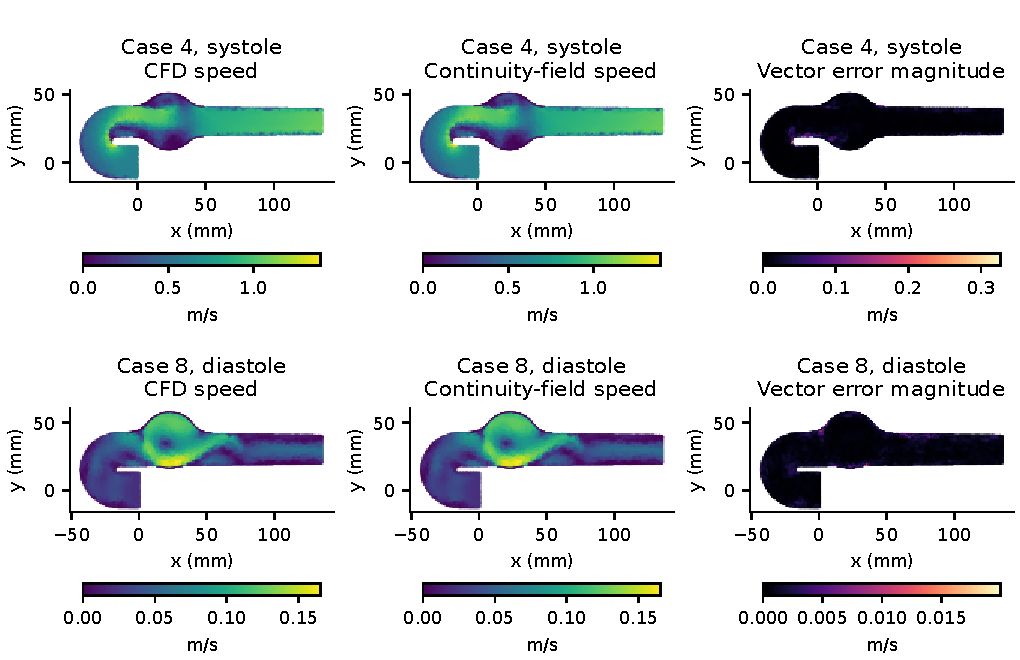
\includegraphics[width=0.90\textwidth]{hidden_velocity_examples.pdf}
\caption{Hidden-node speed on the mid-plane ($|z-z_{\rm mid}|<0.35$~mm) for Case~4 at systole and Case~8 at diastole (draw 0, 2.5~mm). Left, \CFD; center, continuity field; right, magnitude of the vector error. Only unobserved nodes are shown.}
\label{fig:velocity_maps}
\end{figure}

The 99th percentile of aneurysm-zone \WSS is recovered to 0.92 of the \CFD value at systole and 0.90 at diastole, whereas \RBF recovers only 0.52 and 0.61 of it, so \RBF's \WSS error consists mostly of flattened peaks. The Pearson correlation between reconstructed and \CFD \WSS magnitude is 0.92 at systole and 0.94 at diastole for the continuity field, against 0.87 and 0.79 for \RBF, and the \WSS vector errors are 0.38 and 0.20 against 0.62 and 0.42. The systolic pressure drop, which ranges from 413 to 1063~Pa across the cases, is recovered with a median absolute error of 6~Pa against 31~Pa for \RBF. At diastole the median drop errors of 0.48 and 0.67~Pa are comparable to the drops themselves (0.4--5.8~Pa), so neither method recovers the diastolic drop reliably, even though the relative error over the whole pressure field is modest.

The two kinds of error also differ in form. In the median systolic unit (Figure~\ref{fig:field_maps}) the continuity field reproduces the \WSS rings at both necks, while \RBF smears them and underestimates their peaks.

\begin{figure}[H]
\centering
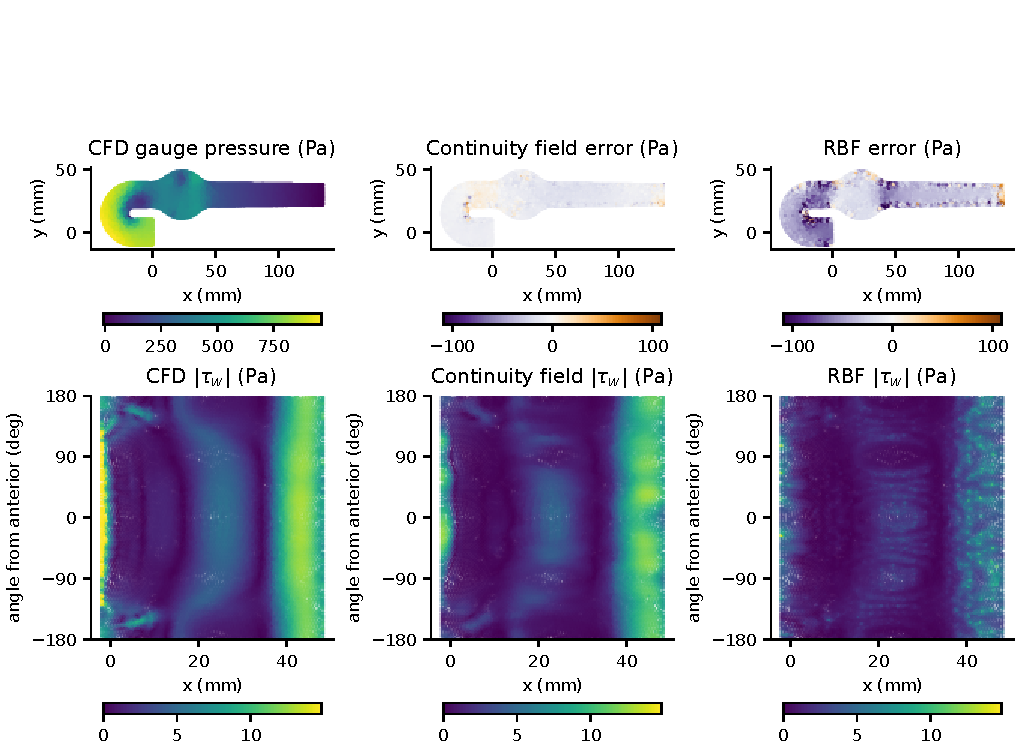
\includegraphics[width=0.95\textwidth]{field_maps_c04_t1780.pdf}
\caption{Case~4 at systole (draw 0, 2.5~mm), close to the median result. Top, \CFD mid-plane pressure and the pressure errors of the continuity field and \RBF. Bottom, aneurysm-zone \WSS unwrapped about the vessel axis. Relative errors are 0.024 and 0.100 for pressure and 0.32 and 0.60 for \WSS.}
\label{fig:field_maps}
\end{figure}

In the adverse diastolic unit (Figure~\ref{fig:field_maps_adverse}), the continuity field's pressure error is a smooth offset of about 1~Pa that accumulates along the vessel, which points to a small bias in the integrated pressure gradient such as the two-snapshot acceleration, while \RBF's pressure errors are concentrated near the sac necks.

\begin{figure}[H]
\centering
\IfFileExists{figures/generated/field_maps_c07_t2400.pdf}{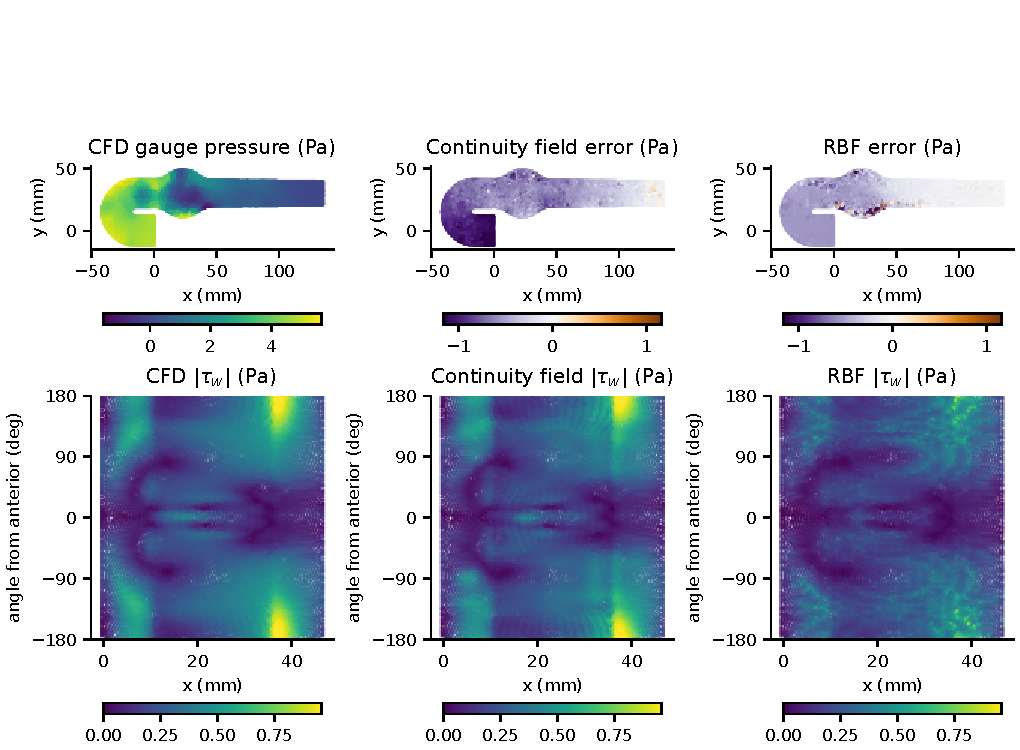
\includegraphics[width=0.95\textwidth]{field_maps_c07_t2400.pdf}}{\fbox{Case 7 diastolic maps pending}}
\caption{As Figure~\ref{fig:field_maps}, for the adverse unit Case~7 at diastole. Relative errors are 0.25 and 0.18 for pressure and 0.14 and 0.33 for \WSS. The \CFD pressure varies by only a few pascals, so errors of about 1~Pa dominate.}
\label{fig:field_maps_adverse}
\end{figure}

The \WSS calculated by automatic differentiation of the continuity field itself was worse than the finite-distance estimate from the same field (median 0.55 against 0.36 in systole and 0.27 against 0.16 in diastole). The soft no-slip penalty fixes the velocity at the wall but leaves its wall-normal gradient poorly determined, so the network's analytic derivative should not be read as \WSS. The finite-distance estimate is also sensitive to $h$. Evaluated at 0.1~mm instead of 0.25~mm, the continuity field's median systolic \WSS error falls from 0.356 to 0.326, and at 0.5~mm it rises to 0.476. We keep the prespecified distance because choosing $h$ with knowledge of the \WSS target would be information that a deployment does not have.

\subsection{Contribution of the continuity penalty and sampling density}
\label{sec:ablation}
Figure~\ref{fig:budget} separates the effect of the continuity penalty from that of the neural representation. At 2.5~mm, the data field without an interior PDE penalty is close to the continuity field, with median velocity errors of 0.052 and 0.039 versus 0.044 and 0.038, and is slightly better on two endpoints, diastolic pressure (0.063 versus 0.094) and systolic \WSS (0.333 versus 0.356). At the densest spacing of 1.5~mm the data field is better on every endpoint except systolic pressure. Only at the sparsest spacing of 4.0~mm, where the observations cover 0.34--0.37\% of the nodes, does the continuity penalty help consistently, reducing the median hidden-velocity error from 0.125 to 0.077 at systole and from 0.105 to 0.077 at diastole, the systolic pressure error from 0.072 to 0.052 and the diastolic \WSS error from 0.371 to 0.316. The main advantage over \RBF therefore comes from fitting one smooth space-time representation to both snapshots, and continuity becomes useful when the data alone no longer determine the field.

The advantage of both neural fields over \RBF grows as the observations become sparser. The median systolic pressure errors at 1.5, 2.5 and 4.0~mm are 0.024, 0.023 and 0.052 for the continuity field versus 0.029, 0.079 and 0.178 for \RBF, and the median systolic \WSS errors are 0.30, 0.36 and 0.48 versus 0.49, 0.61 and 0.68. At diastole and 4.0~mm the continuity field's pressure error is 0.096 versus 0.318 for \RBF. Only one draw was performed at 1.5 and 4.0~mm, so these values describe a trend rather than an uncertainty interval.

\begin{figure}[H]
\centering
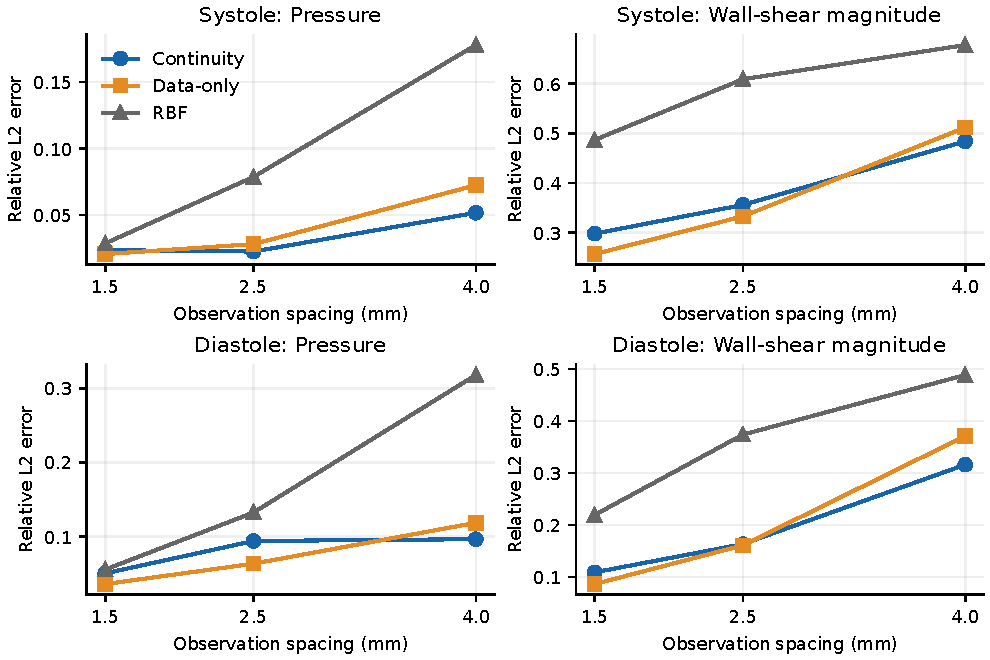
\includegraphics[width=0.92\textwidth]{observation_budget.pdf}
\caption{Median pressure (unsteady form with oracle $\mu_t$) and aneurysm-zone \WSS errors over Cases~2--8 against observation spacing. The 2.5~mm values average three draws per case; 1.5 and 4.0~mm use one draw.}
\label{fig:budget}
\end{figure}

Figure~\ref{fig:pressure_information} asks two separate questions about pressure recovery, namely whether to retain the local acceleration term and whether to supply the \CFD eddy viscosity. Here, steady and unsteady refer to the pressure calculation applied after reconstruction, not to separately trained neural fields. In the seven confirmation geometries, the systolic median improves when the time term is retained and changes little when the eddy viscosity is removed. The unsteady form gives a median error of 0.023 against 0.034 for the steady form, close to the floors of 0.019 and 0.036, and dropping $\mu_t$ changes 0.023 to 0.027. At diastole the eddy viscosity is essential, since removing it more than doubles the continuity field's error, from 0.094 to 0.207, and raises the floor from 0.037 to 0.154. The time term behaves differently for the reconstruction and for the complete \CFD field at diastole. The floor favors the unsteady form (0.037 against 0.065), but the continuity field does better with the steady form (0.072 against 0.094), because the 10~ms finite difference of two reconstructed diastolic fields, whose speeds are about one tenth of the systolic ones, amplifies small reconstruction errors. Diastolic pressure recovery in this setting therefore needs both an estimate of the eddy viscosity and a more accurate acceleration than two sparse snapshots provide.

\begin{figure}[H]
\centering
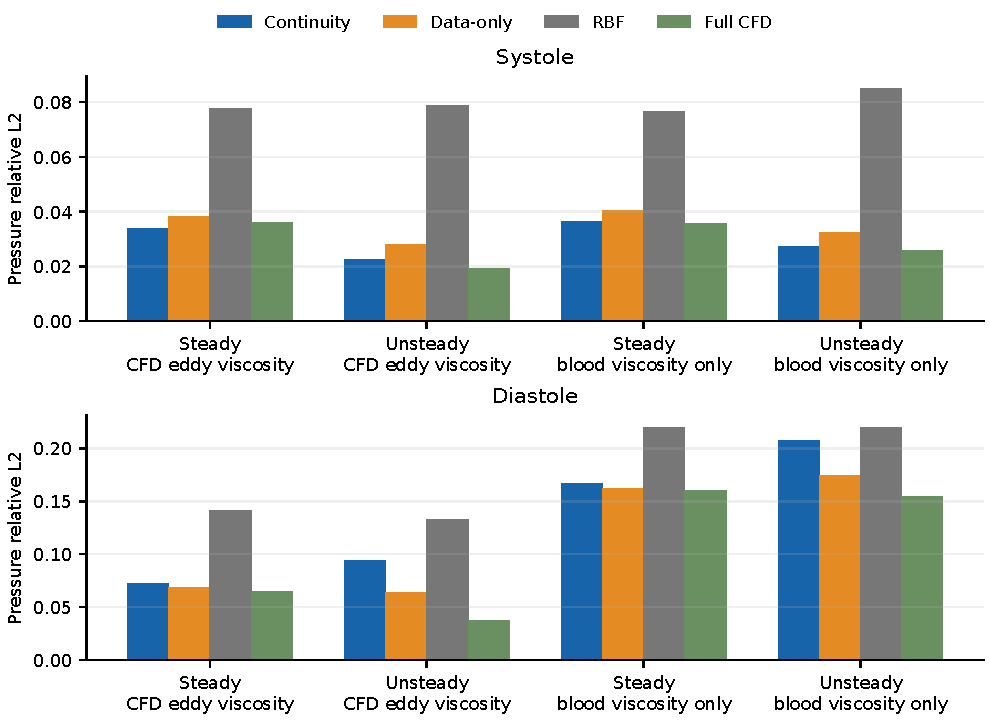
\includegraphics[width=\textwidth]{pressure_information.pdf}
\caption{Median pressure error over Cases~2--8 at 2.5~mm for the four post-processing settings. Unsteady retains the two-snapshot time derivative and steady omits it. ``\CFD eddy viscosity'' uses $\mu+\mu_t$ from the reference simulation, and ``blood viscosity only'' sets $\mu_t=0$. Full \CFD applies the same settings to the complete velocity.}
\label{fig:pressure_information}
\end{figure}

\subsection{Robustness to the choice of interpolation comparator}
\label{sec:robustness}
The prespecified \RBF used one fixed local interpolant in each snapshot. To test how much the comparison depended on that choice, we also evaluated a tuned spatial \RBF and a space-time \RBF, with their settings chosen from the withheld velocity observations. Table~\ref{tab:robustness} reports the completed comparisons for draw 0 at 2.5~mm; these values use one draw per case, so they should be compared within this table rather than directly with the three-draw means of the primary analysis.

At systole, fitting both snapshots with a space-time \RBF changed the median pressure error only slightly, from 0.079 for the prespecified \RBF to 0.074, and the \WSS error from 0.606 to 0.595. The continuity field gave errors of 0.025 and 0.356, respectively, and had lower velocity, pressure and \WSS errors than each \RBF variant in all seven cases. Tuning the spatial \RBF did not improve this phase, since its median pressure and \WSS errors were 0.127 and 0.686; therefore, choosing an interpolant by its velocity error in withheld observations did not ensure lower errors in hidden fields derived from its spatial gradients.

At diastole, both alternatives helped the interpolation. Relative to the prespecified \RBF, the tuned spatial \RBF reduced the median velocity error from 0.129 to 0.100, the pressure error from 0.136 to 0.111 and the \WSS error from 0.371 to 0.321, and the space-time \RBF reduced them to 0.096, 0.113 and 0.301. The continuity field kept lower velocity and \WSS errors than both variants in all seven cases, with a median pressure error of 0.076, but its pressure advantage held in only five of the seven diastolic cases against each variant. Over all 14 case--phase units, the continuity field had the lower pressure error in 12 against the tuned \RBF and in 12 against the space-time \RBF, with median error ratios of 0.50 and 0.54, and the lower \WSS error in all 14 against both, with median ratios of 0.54 and 0.58. It also had a lower pressure error than the better of the two variants in 12 of the 14 units. The comparison against the prespecified \RBF is therefore not an artifact of a weak interpolant, although a stronger interpolant narrows the diastolic pressure gap.

% Generated by generate_robustness_table.py.
\begin{table}[htbp]
\centering
\small
\caption{\revision{\textcolor{red}{Robustness to the interpolation comparator, given as median relative errors over the seven cases in each phase (Cases~2--8) with draw 0 at 2.5~mm. The tuned RBF chooses kernel, neighbourhood and smoothing on the withheld observations, while the space-time RBF interpolates both snapshots jointly with a time scale chosen the same way. All methods share the post-processing, and pressure uses the unsteady form with oracle $\mu_t$.}}}
\label{tab:robustness}
\begin{tabular}{llccc}
\toprule
Phase & Method & Velocity & Pressure & WSS \\
\midrule
Systole & Continuity field & 0.043 & 0.025 & 0.356 \\
Systole & RBF (prespecified) & 0.144 & 0.079 & 0.606 \\
Systole & RBF (tuned) & 0.177 & 0.127 & 0.686 \\
Systole & RBF (space-time) & 0.147 & 0.074 & 0.595 \\
Diastole & Continuity field & 0.038 & 0.076 & 0.173 \\
Diastole & RBF (prespecified) & 0.129 & 0.136 & 0.371 \\
Diastole & RBF (tuned) & 0.100 & 0.111 & 0.321 \\
Diastole & RBF (space-time) & 0.096 & 0.113 & 0.301 \\
\bottomrule
\end{tabular}
\end{table}



\subsection{Sensitivity to near-wall observations}
\label{sec:nearwall}
Because the grid observations are snapped to mesh nodes, some lie on the near-wall prism layers (Section~\ref{sec:observations}). To measure how much the results depend on them, we repeated draw 0 at 2.5~mm for the continuity field and \RBF after removing every observation closer than $\Delta/2=1.25$~mm to the wall, which removed 28--32\% of the observations in each case (Table~\ref{tab:nearwall}). Nothing else was changed.

The \WSS errors rose sharply. For the continuity field the median rose from 0.356 to 0.806 at systole and from 0.173 to 0.521 at diastole, and for \RBF from 0.606 to 0.886 and from 0.371 to 0.681. The accuracy of the one-sided \WSS estimate therefore rests largely on velocity sampled within about a millimetre of the wall, which a 2.5~mm imaging voxel would not resolve. Pressure was much less sensitive. The continuity field's median pressure error changed from 0.025 to 0.027 at systole and from 0.076 to 0.045 at diastole, consistent with pressure being integrated only on nodes more than 1~mm from the wall. The continuity field still had lower velocity, pressure and \WSS errors than \RBF in all 14 units, so the comparison between the methods does not depend on the near-wall samples, whereas the absolute \WSS accuracy does.

% Generated by scripts/manuscript/generate_nearwall_table.py.
\begin{table}[htbp]
\centering
\small
\caption{Sensitivity to near-wall observations. Median relative errors over Cases~2--8 for draw 0 at $\Delta=2.5$~mm, with all observations and with the observations closer than $\Delta/2=1.25$~mm to the wall removed (28--32\% of them). Pressure uses the unsteady form with CFD eddy viscosity; WSS uses $h=0.25$~mm. Velocity is scored on all unobserved nodes, so the second pair of rows is also scored on the removed nodes.}
\label{tab:nearwall}
\begin{tabular}{llccc}
\toprule
Phase & Method and observations & Velocity & Pressure & WSS \\
\midrule
Systole & Continuity field, all observations & 0.043 & 0.025 & 0.356 \\
Systole & RBF, all observations & 0.144 & 0.079 & 0.606 \\
Systole & Continuity field, none within 1.25~mm & 0.130 & 0.027 & 0.806 \\
Systole & RBF, none within 1.25~mm & 0.248 & 0.121 & 0.886 \\
\addlinespace
Diastole & Continuity field, all observations & 0.038 & 0.076 & 0.173 \\
Diastole & RBF, all observations & 0.129 & 0.136 & 0.371 \\
Diastole & Continuity field, none within 1.25~mm & 0.123 & 0.045 & 0.521 \\
Diastole & RBF, none within 1.25~mm & 0.258 & 0.108 & 0.681 \\
\bottomrule
\end{tabular}
\end{table}



\section{Discussion}
\label{sec:discussion}
\subsection{Effects of inlet diameter and asymmetry}
With the flow waveform and the maximum sac diameter held fixed, inlet diameter set the strength of the systolic disturbance and asymmetry set its location. A narrower parent vessel raised the peak Reynolds number, the jet speed entering the sac, the pressure drop, the fraction of reversed flow and the modeled eddy viscosity, and it strengthened the high-shear rings at the necks. This agrees with reports that a larger parent vessel lowers \WSS in intracranial aneurysms~\cite{fattahi2023influence}, and it extends the comparison to transitional flow in a curved, tapered thoracic segment. Because the same flow rate was prescribed for all diameters, the diameter effect here combines the change in geometry with the change in mean velocity. A study that scaled the flow rate with the vessel area would separate these two influences.

Asymmetry moved the low-shear region and the dominant vortex to the side of the larger bulge and shifted the distal high-shear region toward it, while changing the systolic pressure drop by less than 7\%. At diastole its effect became larger than that of diameter, with the asymmetric sacs carrying about two to three times the \WSS of the axisymmetric ones. A previous study of idealized abdominal and descending thoracic aneurysms also found that asymmetry mainly redistributes recirculation and \WSS~\cite{rehman2024comparative}. The present results add that the redistribution depends on the phase of the cycle, so single-instant comparisons at peak systole understate it. None of these comparisons is a population statistic, since each geometry is a single designed case, and whether low or high \WSS relates to growth or rupture cannot be settled by simulations of this kind~\cite{geers2017wall,lipp2020computational}.

\subsection{Why the neural field outperformed interpolation}
The clearest gain came from the reconstructed velocity rather than from adding momentum to the training loss. The neural fields and the prespecified \RBF received the same velocity observations and boundary values, and their pressure and \WSS were computed by the same post-processing. Yet the data field, which has no interior PDE penalty, performed close to the continuity field at 1.5 and 2.5~mm. Both neural fields also retained near-wall gradients that the prespecified \RBF tended to smooth out, and their finite-distance shear estimates recovered about 90--100\% of the \CFD 99th-percentile \WSS, compared with about half for \RBF at systole. The continuity penalty became consistently useful at the sparsest spacing, 4.0~mm.

The network fits one function across the domain and both snapshots, whereas the prespecified \RBF uses a local neighborhood at each time. This difference offers a plausible explanation for the results, but the study does not isolate the effects of spatial smoothness, joint temporal fitting and the network architecture. The space-time \RBF check narrows that interpretation, because fitting both snapshots jointly did not close the gap to the neural field at systole. At diastole, both tuning and joint temporal fitting improved all three median errors of the interpolant and reduced the continuity field's pressure advantage to five of seven cases for draw 0. These checks support the use of a neural representation in this setting without establishing that it is preferable to every interpolation scheme. Related work has used implicit neural representations for 4D flow reconstruction without a physics loss~\cite{saitta2024implicit}; here, the representation supplies velocity to the established momentum-integration route for relative pressure~\cite{krittian2012finite,bertoglio2018relative}.

The momentum \PINNs did not meet the criterion of the development test. Their poor pressure outputs, despite small momentum residuals, are consistent with a weakly determined trade-off between pressure and local acceleration. Two velocity snapshots constrain a finite difference, but they do not uniquely determine the network's time derivative between them. The diagnostic in Section~\ref{sec:pilot_results} showed that a small residual could coexist with an inaccurate pressure field. This fits the broader sensitivity of \PINNs to loss weighting and the information available to each residual~\cite{krishnapriyan2021failure,wang2021gradient}. Recovering pressure after fitting avoids relying on that pressure head, although the two-snapshot acceleration still carries reconstruction error. Longer time series, hard constraints and other loss weights might change the comparison. They were not tested here, so the negative result applies to the specified formulation and windows rather than to momentum \PINNs in general~\cite{mcgreivy2024weak}.

\subsection{Information needed for each hidden field}
Pressure and \WSS expose different weaknesses in the reconstruction of the sparse velocity. For the seven confirmation geometries, the retention of local acceleration brought the median systolic pressure error close to the complete-\CFD post-processing reference. Removing eddy viscosity did little to change that median, although the reference study of all-cases showed greater sensitivity in narrower geometries of 2.0~cm. The limited systolic sensitivity of the median should therefore not be read as evidence that eddy viscosity can always be neglected.

At diastole, omitting the \CFD eddy viscosity raised even the complete-velocity pressure error to 9--19\%. The reconstruction results with that field supplied describe a conditional calculation, because the sparse velocity observations do not themselves provide the closure. Small absolute pressure errors also matter more in this phase. None of the tested methods reliably recovered the diastolic pressure drop, even when its relative error across the field appeared modest. An estimate of eddy viscosity and a better-resolved acceleration are, therefore, separate requirements to examine before applying this calculation to measured data.

For aneurysm-zone \WSS, near-wall sampling remained the main limitation. Removing the observations within 1.25~mm of the wall more than doubled the continuity field's \WSS error at both phases while leaving the ranking against \RBF unchanged (Section~\ref{sec:nearwall}). The error depended on the distance used by the one-sided estimate, and the reconstructed fields remained above the complete-\CFD reference. Outside the aneurysm zone, the interior node closest to the wall was a median of 0.58~mm from it; even the complete \CFD velocity then gave a poor estimate of the exported shear. This is consistent with the documented sensitivity of velocity-derived \WSS to spatial resolution~\cite{petersson2012assessment,stalder2008quantitative}. A smooth velocity fit and an analytic derivative do not, by themselves, establish an accurate wall gradient.

\subsection{Limitations}
\label{Limitations}
The twelve geometries form a designed family, not a patient cohort. They share one maximum aneurysm diameter, taper ratio and inflow waveform, and they contain no branches. The seven confirmation geometries therefore test variation within that family. The rigid-wall flow solution has reported mesh, time-step and cycle checks for aneurysm \WSS, but no experimental validation. The structural calculation uses a uniform 2~mm wall, literature material parameters, fixed ends and a quasi-static coupling. Its coupling-step and mesh-update settings were not retained with the results, and no solid-mesh convergence check is available, so the stress fields are used only to describe modeled stress concentrations.

The temporal records also have limits. Each reconstruction uses two snapshots from a short window. Several instants were retained, but no complete cycle-resolved wall-traction series is available. The solver exported \TAWSS to the wall nodes, but its cycle-resolved components did not, so the oscillatory indices were not evaluated. The slice workbook does not state its averaging interval; the slice values were identified as cycle averages from the inlet flow rate.

The observed velocities are noise-free \CFD values at the mesh nodes. They do not include partial-volume averaging, noise, segmentation error, or velocity aliasing of 4D flow MRI~\cite{markl2012fourd}, and some lie within a fraction of a millimeter of the wall (Section~\ref{sec:observations}). Without observations within 1.25~mm of the wall, the \WSS errors were more than twice as large (Section~\ref{sec:nearwall}), so the absolute \WSS precision reported here should not be expected from the imaging data. Performance on measured data may therefore be worse. Pressure calculations with \CFD-supplied eddy viscosity additionally assume closure information that would have to be estimated in practice. The errors are node-weighted because the exports contain no cell volumes, which gives a greater weight to the refined near-wall mesh.

The network architecture and training settings were fixed on the development cases without a wider hyperparameter search. The tuned and space-time \RBF checks were added after the primary verdict and use one draw per case; they cannot replace the three-draw comparison. A divergence-free interpolant, the natural non-neural counterpart of the continuity field, was not tested. Every method receives observations in the target geometry. The prediction in a geometry with no observations was not tested. Finally, fitting a neural field took about 20~min on a GPU per window, so its accuracy came at a higher computational cost than interpolation.

\section{Conclusion}
\label{sec:conclusion}
Twelve idealized descending thoracic aortic geometries with a fixed maximum sac diameter of 4.0~cm were simulated with transient transitional \CFD, and their common-time fields were used both to compare the geometries and to test the recovery of hidden pressure and \WSS from sparse velocity. The inlet diameter dominated the systolic response. Reducing it from 2.6 to 2.0~cm raised the pressure drop 2.3--2.5 times, roughly doubled the fraction of reversed flow in dilation, and raised the 95th-percentile \WSS in the necks from 7--8 to 15--18~Pa, while the bulge pattern changed the drop in systolic pressure by less than 7\%. Instead, asymmetry relocated the low-shear region and the dominant vortex to the larger bulge, and at diastole it raised the median \WSS of the dilation segment 1.8--3.1 times relative to the axisymmetric sacs.

With velocity observed at about 1.3\% of the interior nodes at two instants, a continuity-constrained space-time neural field followed by momentum integration and a near-wall shear estimate recovered pressure and aneurysm-zone \WSS more accurately than the same post-processing applied to the prespecified \RBF in all 14 confirmation units after averaging three draws per unit, with median error ratios of 0.46 and 0.51. The pressure advantage was small at diastole. The benefit came mainly from the neural representation of the velocity. A continuity penalty helped in the sparsest sampling, and momentum \PINNs did not meet the development-test criterion for joint pressure and shear recovery. Systolic pressure was recovered close to the accuracy of post-processing itself, diastolic pressure required the \CFD eddy viscosity as an input to the oracle, and \WSS accuracy depended on the velocity sampled close to the wall, although the continuity field retained its advantage over \RBF without those samples. These findings identify what information each hidden field needs in this idealized, noise-free setting. Measured velocity data, estimated closures, and patient-specific anatomies are the next tests, and none of the results constitutes a clinical rupture-risk assessment.

\section*{Declarations}
\paragraph{Conflicts of interest.} The authors have no conflicts to disclose.

\ifanonymized
\paragraph{Funding and author contributions.} Removed for anonymized review.
\else
\paragraph{Funding.} Helmi Temimi thanks the Kuwait Foundation for the Advancement of Sciences (Project Code: CN22-16QE-1643).

\paragraph{Author contributions.} Conceptualization, M.A.U.R. and M.A.O.; \CFD and structural modeling, M.A.U.R.; reconstruction methodology, software and formal analysis of the reconstruction study, M.A.O.; validation, M.A.U.R., M.A.O., F.J. and H.T.; data curation, M.A.U.R. and M.A.O.; writing (original draft), M.A.U.R. and M.A.O.; writing (review and editing), all authors; funding acquisition, F.J. and H.T. All authors have read and agreed to the submitted version.
\fi


% \paragraph{Use of generative AI.} During the preparation of this work, the authors used Claude (Anthropic) and Codex (OpenAI) to help write and edit the language and grammar of the manuscript. The simulations, the study design and the interpretation of the results are the authors' own. The authors reviewed and edited all AI-assisted output and take full responsibility for the content of the publication.

\paragraph{Data availability statement.} The \CFD exports analyzed in this study are available from the corresponding author on reasonable request. \ifanonymized The reconstruction code and configuration files are available in a public repository whose link is withheld for anonymized review.\else The reconstruction code and configuration files are available at \url{https://github.com/michaelajao/IdealAorta-PINN}.\fi

\appendix
\section{Case-wise reconstruction results}
\label{app:casewise}
Tables~\ref{tab:case_pressure} and \ref{tab:case_shear} list every confirmation unit at 2.5~mm, spread over the three paired draws and the range of draw-wise error ratios to \RBF.

\begin{table}[htbp]
\centering
\small
\caption{Case-wise pressure relative L2 at 2.5~mm, given as the mean (sample standard deviation) over three paired observation/initialization draws. The last column is the range of draw-wise continuity/RBF error ratios, and values above one favor RBF. The spread describes these draws, not patient-population uncertainty.}
\label{tab:case_pressure}
\begin{tabular}{llcccc}
\toprule
Case & Phase & Continuity & Data-only & RBF & Ratio range \\
\midrule
2 & Sys. & 0.069 (0.004) & 0.069 (0.008) & 0.111 (0.010) & 0.53--0.68 \\
2 & Dia. & 0.094 (0.026) & 0.050 (0.012) & 0.138 (0.016) & 0.55--0.81 \\
3 & Sys. & 0.031 (0.004) & 0.030 (0.004) & 0.078 (0.009) & 0.35--0.47 \\
3 & Dia. & 0.028 (0.004) & 0.032 (0.003) & 0.095 (0.014) & 0.27--0.32 \\
4 & Sys. & 0.023 (0.001) & 0.027 (0.008) & 0.093 (0.019) & 0.20--0.30 \\
4 & Dia. & 0.107 (0.032) & 0.071 (0.020) & 0.157 (0.018) & 0.50--1.05 \\
5 & Sys. & 0.022 (0.002) & 0.028 (0.002) & 0.079 (0.011) & 0.24--0.31 \\
5 & Dia. & 0.044 (0.017) & 0.059 (0.027) & 0.113 (0.015) & 0.29--0.56 \\
6 & Sys. & 0.020 (0.000) & 0.027 (0.004) & 0.081 (0.017) & 0.20--0.30 \\
6 & Dia. & 0.085 (0.029) & 0.093 (0.031) & 0.132 (0.004) & 0.51--0.89 \\
7 & Sys. & 0.021 (0.004) & 0.022 (0.003) & 0.074 (0.015) & 0.25--0.34 \\
7 & Dia. & 0.155 (0.085) & 0.090 (0.035) & 0.171 (0.008) & 0.54--1.40 \\
8 & Sys. & 0.032 (0.005) & 0.030 (0.009) & 0.063 (0.007) & 0.50--0.54 \\
8 & Dia. & 0.101 (0.076) & 0.063 (0.011) & 0.104 (0.005) & 0.31--1.75 \\
\bottomrule
\end{tabular}
\end{table}

\begin{table}[htbp]
\centering
\small
\caption{Case-wise wall-shear magnitude relative L2 at 2.5~mm, given as the mean (sample standard deviation) over three paired observation/initialization draws. The last column is the range of draw-wise continuity/RBF error ratios, and values above one favor RBF. The spread describes these draws, not patient-population uncertainty.}
\label{tab:case_shear}
\begin{tabular}{llcccc}
\toprule
Case & Phase & Continuity & Data-only & RBF & Ratio range \\
\midrule
2 & Sys. & 0.417 (0.007) & 0.386 (0.018) & 0.653 (0.004) & 0.63--0.65 \\
2 & Dia. & 0.166 (0.009) & 0.169 (0.029) & 0.404 (0.002) & 0.39--0.43 \\
3 & Sys. & 0.363 (0.010) & 0.333 (0.026) & 0.636 (0.008) & 0.55--0.60 \\
3 & Dia. & 0.166 (0.006) & 0.148 (0.013) & 0.409 (0.005) & 0.39--0.43 \\
4 & Sys. & 0.329 (0.033) & 0.306 (0.018) & 0.605 (0.001) & 0.51--0.61 \\
4 & Dia. & 0.131 (0.004) & 0.150 (0.020) & 0.302 (0.002) & 0.42--0.44 \\
5 & Sys. & 0.356 (0.005) & 0.359 (0.011) & 0.619 (0.010) & 0.56--0.59 \\
5 & Dia. & 0.163 (0.018) & 0.174 (0.008) & 0.386 (0.001) & 0.37--0.45 \\
6 & Sys. & 0.373 (0.002) & 0.352 (0.027) & 0.609 (0.005) & 0.61--0.62 \\
6 & Dia. & 0.155 (0.030) & 0.161 (0.008) & 0.368 (0.003) & 0.33--0.50 \\
7 & Sys. & 0.323 (0.012) & 0.300 (0.011) & 0.590 (0.005) & 0.53--0.57 \\
7 & Dia. & 0.136 (0.004) & 0.146 (0.019) & 0.332 (0.005) & 0.40--0.43 \\
8 & Sys. & 0.330 (0.012) & 0.327 (0.009) & 0.598 (0.005) & 0.54--0.58 \\
8 & Dia. & 0.176 (0.022) & 0.196 (0.013) & 0.374 (0.005) & 0.40--0.51 \\
\bottomrule
\end{tabular}
\end{table}


\newpage
\bibliographystyle{unsrt}
\bibliography{bib/tsb,bib/references}

\end{document}
"
\newif\ifanonymized
\ifdefined\anonymized\anonymizedtrue\fi

\begin{document}

\begin{center}

{\Large \bf
% Hemodynamics of Idealized Descending Thoracic Aortic Aneurysms and Physics-Based Recovery of Pressure and Wall Shear Stress from Sparse Velocity

Effects of Inlet Diameter and Sac Asymmetry on Transitional Flow in Idealized Descending Thoracic Aortic Aneurysms, with Neural-Field Recovery of Pressure and Wall Shear Stress from Sparse Velocity
}\\[12mm]

% Continuity-Constrained Space-Time Neural Fields Improve Pressure and Wall Shear Stress Recovery from Sparse Velocity in Idealized Descending Thoracic Aortic Aneurysms

\ifanonymized\else
{\bf
M. Abaid Ur Rehman$^{a,b,*}$,
{Michael Ajao-Olarinoye$^{c}$},
Fei Jia$^{a,**}$,
Helmi Temimi$^{d}$
}\\[3mm]

{$^{a}$Department of Astronautical Science and Mechanics,
Harbin Institute of Technology, Harbin 150001, China}\\

{$^{b}$Department of Mathematics, School of Natural Sciences (SNS),
National University of Sciences and Technology (NUST),
Sector H-12, 44000, Islamabad, Pakistan}\\

{
$^{c}$Computational Science and Mathematical Modelling (CSMM),
Coventry University, Coventry, United Kingdom
}\\

{$^{d}$College of Integrative Studies,
Abdullah Al Salem University, Khaldiya, Kuwait}\\[3mm]
\fi

\end{center}

\ifanonymized\else
\noindent
$^{*}$\textbf{Corresponding author:}
M. Abaid Ur Rehman,
Email:
\href{mailto:abaidurrehman803@gmail.com}
{abaidurrehman803@gmail.com}

\vspace{1mm}

\noindent
$^{**}$\textbf{Corresponding author:}
Fei Jia,
Email:
\href{mailto:jiafei0009@163.com}
{jiafei0009@163.com}

\vspace{3mm}

\begin{center}
\textbf{Emails:}
\href{mailto:abaidurrehman803@gmail.com}
{abaidurrehman803@gmail.com},
{
\href{mailto:ajaoolarinoyemichael@gmail.com}
{ajaoolarinoyemichael@gmail.com}},
\href{mailto:jiafei0009@163.com}
{jiafei0009@163.com},
\href{mailto:helmi.temimi@aasu.edu.kw}
{helmi.temimi@aasu.edu.kw}
\end{center}
\fi

\begin{abstract}
We examined how inlet diameter and sac asymmetry affect flow in twelve idealized \DTAA geometries, then used their \CFD fields to test pressure and \WSS recovery from sparse velocity. Nine aneurysmal models combined three inlet diameters (2.0, 2.3 and 2.6~cm) with axisymmetric, anterior-dominant and posterior-dominant sacs; three models served as controls. All aneurysms had a maximum diameter of 4.0~cm, and all vessels had an outlet-to-inlet diameter ratio of 0.8. At a fixed flow waveform, narrowing the inlet from 2.6 to 2.0~cm increased systolic pressure drop from 528--561 to 1261--1346~Pa and the 95th-percentile \WSS from 7--8 to 15--18~Pa. Asymmetry mainly changed the location of low shear and increased diastolic segment-median \WSS by a factor of 1.8--3.1 relative to axisymmetric sacs. Reconstruction used noise-free velocity sampled at about 1.3\% of interior nodes at two instants 5--10~ms apart. Interpolation and space-time neural fields were compared using shared pressure and shear calculations. In seven evaluation geometries, the continuity-constrained field reduced pressure and \WSS errors relative to the prespecified \RBF in all 14 case--phase means, with median error ratios of 0.46 and 0.51. Most of the benefit came from the neural representation; momentum-constrained \PINNs tested on two development geometries did not improve joint pressure and shear recovery. Diastolic pressure estimates depended on \CFD-supplied eddy viscosity, and \WSS accuracy deteriorated when near-wall observations were removed. These results characterize reconstruction in known, idealized geometries; they do not establish performance on measured data or clinical rupture risk.
\end{abstract}
\acresetall

\noindent\textbf{Keywords.} Thoracic aortic aneurysm; computational fluid dynamics; wall shear stress; sparse flow reconstruction; physics-informed neural networks; relative pressure estimation


\section{Introduction}
\label{sec:introduction}

Descending thoracic aortic aneurysms alter both blood flow and the mechanical loading of the vessel wall. Their geometry varies in parent-vessel size, curvature and sac asymmetry. These features can differ even when two aneurysms have the same maximum diameter, motivating comparisons that control diameter while varying the surrounding geometry~\cite{lipp2020computational,vorp1998mechanical}.

Maximum diameter is an important clinical measure, but it does not describe wall thickness, tissue properties or the full aneurysm shape. Evidence from abdominal aortic aneurysms shows that diameter alone does not determine rupture~\cite{darling1977autopsy} and has motivated complementary volumetric measures~\cite{kitagawa2013role}. These observations motivate biomechanical analysis, but findings from abdominal or cerebral aneurysms cannot by themselves establish rupture predictors for \DTAA. Structural tensile stress and hemodynamic \WSS also describe different loads: local wall failure depends on the relation between tissue stress and tissue strength, whereas \WSS characterizes tangential loading by blood flow~\cite{vorp1998mechanical,bilgi2020effects}.

\CFDcap estimates velocity, pressure and shear fields that are difficult to measure throughout an aneurysm~\cite{lee2011computational,morris2016computational}. Common descriptors include \WSS, \WSSG, \TAWSS and \OSI. Their associations with disease depend on the anatomy and outcome studied. Geers et al.~\cite{geers2017wall}, for example, examined shear at cerebral aneurysm initiation sites, whereas Moon et al.~\cite{moon2025hemodynamic} reported low \TAWSS and elevated oscillatory and residence-time indices at rupture regions in four infrarenal aneurysms. Such findings motivate spatial hemodynamic comparisons without establishing a validated rupture model for the idealized thoracic geometries studied here.

Parent-vessel diameter and curvature affect the jet entering an aneurysm and the resulting recirculation. Studies of tortuous arteries have linked these geometric features to changes in shear and residence-time indices~\cite{10a,11a,12a,13a,14a}. In intracranial aneurysm models, larger parent-vessel diameters reduced \WSS and \OSI~\cite{fattahi2023influence,fattahi2023usage}, while changes in aspect and size ratios altered near-neck hemodynamics~\cite{nagargoje2022influence}. A controlled thoracic-aorta model allows these geometric effects to be examined without the simultaneous anatomical variation present in patient cohorts.

Pulsatility, curvature and sac expansion can produce transitional flow, making the choice of flow model relevant to the calculated hemodynamics~\cite{brambila2023influence,evju2015assumption,luciano2024turbulent,rawat2019numerical}. Reynolds-averaged turbulence models represent the effects of unresolved fluctuations through a closure; \DNS instead resolves the turbulent scales directly. Here we use the transition \SST $k$--$\omega$ model to represent possible laminar--turbulent transition. The resulting turbulence quantities are model predictions and require validation before being interpreted as measurements of physiological turbulence.

Several studies have investigated aneurysm hemodynamics using patient-based and idealized geometries. Lauric et al.~\cite{lauric2019proximal} examined 33 middle cerebral artery aneurysm patients and 44 controls, finding aneurysmal arteries have a tapered parent vessel (mean ratio 0.88) versus near-unity in healthy vessels; tapering elevates \WSS and \WSSG, promoting aneurysm formation. Jin et al.~\cite{jin2023cfd} reported that reducing coil porosity from 0.89 to 0.79 decreases \OSI by up to 55\% in an \ICA aneurysm. Tian et al.~\cite{tian2023influence} used 18 idealized and 7 patient-specific bifurcation aneurysms to show that the aneurysm--parent vessel angle dominates \LDL deposition, with larger angles promoting deposition by reducing inflow and enhancing stagnation. Rehman et al.~\cite{ur2025fluid} studied Marfan syndrome aneurysms using \FSI with \CFD and \PINNs on six patient-specific models, observing that \WSS disturbances vary with shape and that the anterior wall experiences higher stresses. Zhou et al.~\cite{zhou2026morphological} developed an AutoML model on 158 intracranial aneurysms, identifying bifurcation angle as the most critical risk factor. These patient-based studies, however, are confounded by multiple simultaneously varying anatomical features, making it difficult to isolate single-parameter effects. Idealized geometries offer systematic parameter variation.

The present study examines a curved, tapered family of twelve idealized descending thoracic aortas (Table~\ref{tab:lit_review}). Nine aneurysmal geometries combine inlet diameters of 2.0, 2.3 and 2.6~cm with axisymmetric, anterior-dominant and posterior-dominant sacs; three nonaneurysmal geometries provide matched controls. The maximum sac diameter is fixed at 4.0~cm, and every vessel has an outlet-to-inlet diameter ratio of 0.8. This design compares inlet diameter and bulge direction under a common taper and flow waveform. Because taper is fixed, the study does not estimate the effect of changing taper itself.

The same \CFD fields support a second question: how accurately can pressure and \WSS be recovered from sparse velocity in a known geometry? Time-resolved three-dimensional phase-contrast MRI (4D flow MRI) samples velocity on voxels of roughly one to three millimeters~\cite{markl2012fourd}; pressure and wall shear must be estimated from those measurements. Relative-pressure methods use the momentum balance~\cite{krittian2012finite,bertoglio2018relative}, while velocity-derived \WSS is sensitive to resolution and wall segmentation~\cite{stalder2008quantitative,petersson2012assessment,potters2015volumetric}. Neural fields provide a continuous velocity representation, optionally constrained by the governing equations~\cite{raissi2019pinn,raissi2020hfm}. Applications include arterial pressure inference~\cite{kissas2020machine}, 4D flow reconstruction~\cite{fathi2020super,saitta2024implicit}, near-wall flow recovery~\cite{arzani2021nearwall} and aneurysm flow reconstruction~\cite{cruzgonzalez2025aaa}. Their performance depends on the observations, training procedure and comparator~\cite{krishnapriyan2021failure,wang2021gradient,mcgreivy2024weak}.

We separate the benefit of the neural representation from that of the physics terms in its loss. We also test which additional inputs pressure and shear recovery require. In unsteady Reynolds-averaged flow, the pressure gradient depends on acceleration and the eddy-viscosity closure as well as velocity. All methods therefore use the same sampled observation pool and shared pressure and shear calculations, with closure information reported explicitly. Table~\ref{tab:lit_review} places this comparison alongside earlier idealized-aneurysm studies.


\begin{table}[htbp]
\centering
\footnotesize
\caption{Comparison of existing idealized aneurysm studies and the present work, emphasizing differences in geometry, flow modeling, boundary conditions, hemodynamic--morphometric analysis, and sparse-velocity reconstruction.}
\setlength{\tabcolsep}{3pt}
\begin{tabular}{|>{\raggedright\arraybackslash}p{4.0cm}|*{6}{>{\centering\arraybackslash}p{1.78cm}|}}
\hline
\textbf{Feature} & \parbox{1.78cm}{\textbf{Jin et al.~\cite{jin2021arterial}}} & \parbox{1.78cm}{\textbf{Guerrero-Hurtado et al.~\cite{guerrero2023efficient}}} & \parbox{1.78cm}{\textbf{Rehman et al.~\cite{rehman2024comparative}}} & \parbox{1.78cm}{\textbf{Rehman et al.~\cite{rehman2025application}}} & \parbox{1.78cm}{\textbf{Moroni \& Espa~\cite{moroni2025insight}}} & \parbox{1.78cm}{\textbf{Present Study}} \\
\hline
Year & 2021 & 2023 & 2024 & 2025 & 2025 & - \\
\hline
Geometry Type & Idealized & Idealized & Idealized & Idealized & Idealized & Idealized \\
\hline
\DTAA & No & No & Yes & No & No & Yes \\
\hline
{Arterial Tapering} & No & No & No & No & No & Yes \\
\hline
Parent vessel effect & No & No & No & No & No & Yes \\
\hline
\parbox{3.7cm}{Morphology: Axisymmetric or Asymmetric} & Not varied & Not varied & Both & Both & Both & Both \\
\hline
\parbox{3.7cm}{SST $k-\omega$ Transition Turbulence Model} & No & No & No & No & No & Yes \\
\hline
Transient Flow Inlet & Yes & Yes & No & No & No & Yes \\
\hline
\parbox{3cm}{Transient Pressure Outlet} & Yes & No & No & No & No & Yes \\
\hline
Plane-wise flow--morphometry analysis & Partial & No & No & Partial & Partial & Yes \\
\hline
\PINNcap & No & No & Yes & No & No & Tested on two cases \\
\hline
Hidden pressure and \WSS from sparse velocity against matched baselines & No & No & No & No & No & Yes \\
\hline
\end{tabular}%
\label{tab:lit_review}
\end{table}



This study addresses both questions on a family of twelve idealized descending thoracic aortic geometries, namely nine aneurysmal models formed by three inlet diameters and three bulge patterns at a fixed 4.0~cm maximum sac diameter, and three nonaneurysmal controls. The contributions are as follows.
\begin{enumerate}
\item We report how inlet diameter and sac asymmetry change pressure drop, reversed flow, eddy viscosity and aneurysm-zone \WSS in transient transitional \CFD, evaluated at common systolic and diastolic instants for all twelve geometries.
\item We define a sparse-reconstruction task on the same fields, in which velocity is observed at about 1.3\% of the interior nodes at two instants 5--10~ms apart and hidden pressure and aneurysm-zone \WSS must be recovered in the known geometry. Linear interpolation, \RBF interpolation and space-time neural fields with and without a continuity penalty all pass through the same momentum-integration and near-wall shear calculations, so their differences are attributable to the reconstructed velocity alone.
\item Using a protocol fixed on two development geometries before evaluation on seven others, we separate the contributions of the neural representation, the continuity constraint, the local time derivative and the eddy-viscosity closure. On two development geometries, we also report that the pressure output of a \PINN with the momentum residual in its loss was far less accurate than momentum integration applied after fitting.
\end{enumerate}
The geometry study supplies reference flows with different jet strengths, recirculation patterns and modeled eddy viscosities. The reconstruction study tests recovery across those conditions. Each reconstruction receives observations in its target geometry; it does not predict flow in an anatomy without observations or estimate clinical rupture risk.


\section{\label{Material and Methods}Materials and methods}
\subsection{\label{Geometric Description}Geometric description}
Twelve idealized descending-aortic geometries were examined, namely nine aneurysmal models and three nonaneurysmal (healthy) controls. The aneurysmal group used three inlet diameters, 2.0, 2.3 and 2.6~cm. An axisymmetric and two asymmetric aneurysm shapes were studied for each inlet diameter. The level of asymmetry was calculated as the ratio $\beta = r/R$, where $r$ and $R$ denote the characteristic radii of the aneurysmal segment in the posterior and anterior directions, respectively. An axisymmetric bulge gives $\beta = 1$; {a} posterior-dominant bulge gives $\beta > 1$ and {an} anterior-dominant bulge $\beta < 1$, the two representing opposite directional dilations. The detailed geometric parameters are given in Table~\ref{tab:geometries}. To compare with the healthy models, the other three models that have the same inlet diameters (2.0~cm, 2.3~cm and 2.6~cm) were also built. In these control cases no aneurysmal dilation was added and, as in the aneurysmal models, the vessels were tapered smoothly along their lengths, with a physiologically consistent reduction in diameter so that the outlet diameter is 80\% of the inlet diameter. The twelve cases therefore form three groups by inlet diameter, each containing three aneurysmal cases and their matching control. Group~1 (2.0~cm) comprises Cases~1--3 and control Case~10, Group~2 (2.3~cm) comprises Cases~4--6 and control Case~11, and Group~3 (2.6~cm) comprises Cases~7--9 and control Case~12. Case numbers are used throughout, and each control is compared with the aneurysmal cases of its own group.

The eight cross-sectional planes (D1--D8) shown in Figure~\ref{fig:diagram} were used to investigate the spatial variations of the hemodynamic parameters along the arterial axis. All the aneurysmal models had a single dilation centered at the mid-region (D5) and the maximum aneurysm diameter was set at 4.0~cm for all the diseased aneurysm cases. The (D1--D4) and (D6--D8) represent the upstream and downstream portions of the aneurysms. The average diameters of the planes are listed in Table~\ref{tab:diameter}. Two section planes are used throughout, the medial plane ($xy$-plane) and the transverse plane ($xz$-plane) through the axis of the descending segment. Every model is mirror-symmetric about the medial plane, and the anterior--posterior asymmetry of the bulge lies within that plane.



\begin{table}[htbp]
\centering
\caption{\AANcap models considered in the present study. Here $r$ and $R$ are the {posterior and anterior} characteristic radii of the sac and $\beta = r/R$ is the directional asymmetry ratio. Each group collects the three aneurysmal cases of one inlet diameter and their control.}
\label{tab:geometries}
\setlength{\tabcolsep}{4pt}
\begin{tabular}{ll ccc ccc}
\toprule
& & \multicolumn{3}{c}{Sac geometry}
  & \multicolumn{3}{c}{Case ID by inlet diameter \(D_{\mathrm{in}}\)} \\
\cmidrule(lr){3-5} \cmidrule(lr){6-8}
& & & & & Group~1 & Group~2 & Group~3 \\
Type & Configuration & \(r\) (cm) & \(R\) (cm) & \(\beta = r/R\)
     & 2.0 cm & 2.3 cm & 2.6 cm \\
\midrule
Axisymmetric & --         & 2.0 & 2.0 & 1.00 & 1  & 4  & 7  \\
Asymmetric   & Ant.-dom.  & 1.3 & 2.7 & 0.48 & 2  & 5  & 8  \\
             & Post.-dom. & 2.7 & 1.3 & 2.08 & 3  & 6  & 9  \\
Control      & --         & --  & --  & --   & 10 & 11 & 12 \\
\bottomrule
\end{tabular}
\end{table}
\begin{table}[htbp]
\centering
\caption{Plane diameter (cm), mean $\pm$ standard deviation across the nine aneurysmal and three control geometries.}
\begin{tabular}{lcc}
\toprule
Plane & Aneurysmal ($n=9$) & Control ($n=3$) \\
\midrule
D1 & 2.28 $\pm$ 0.26 & 2.28 $\pm$ 0.30 \\
D2 & 2.22 $\pm$ 0.25 & 2.22 $\pm$ 0.29 \\
D3 & 2.15 $\pm$ 0.24 & 2.15 $\pm$ 0.28 \\
D4 & 2.97 $\pm$ 0.09 & 2.11 $\pm$ 0.28 \\
D5 & 4.00 $\pm$ 0.00 & 2.08 $\pm$ 0.27 \\
D6 & 2.92 $\pm$ 0.09 & 2.05 $\pm$ 0.27 \\
D7 & 2.02 $\pm$ 0.23 & 2.02 $\pm$ 0.26 \\
D8 & 1.95 $\pm$ 0.22 & 1.95 $\pm$ 0.25 \\
\bottomrule
\end{tabular}
\label{tab:diameter}
\end{table}


 \begin{figure}[ht!]
         \centering
         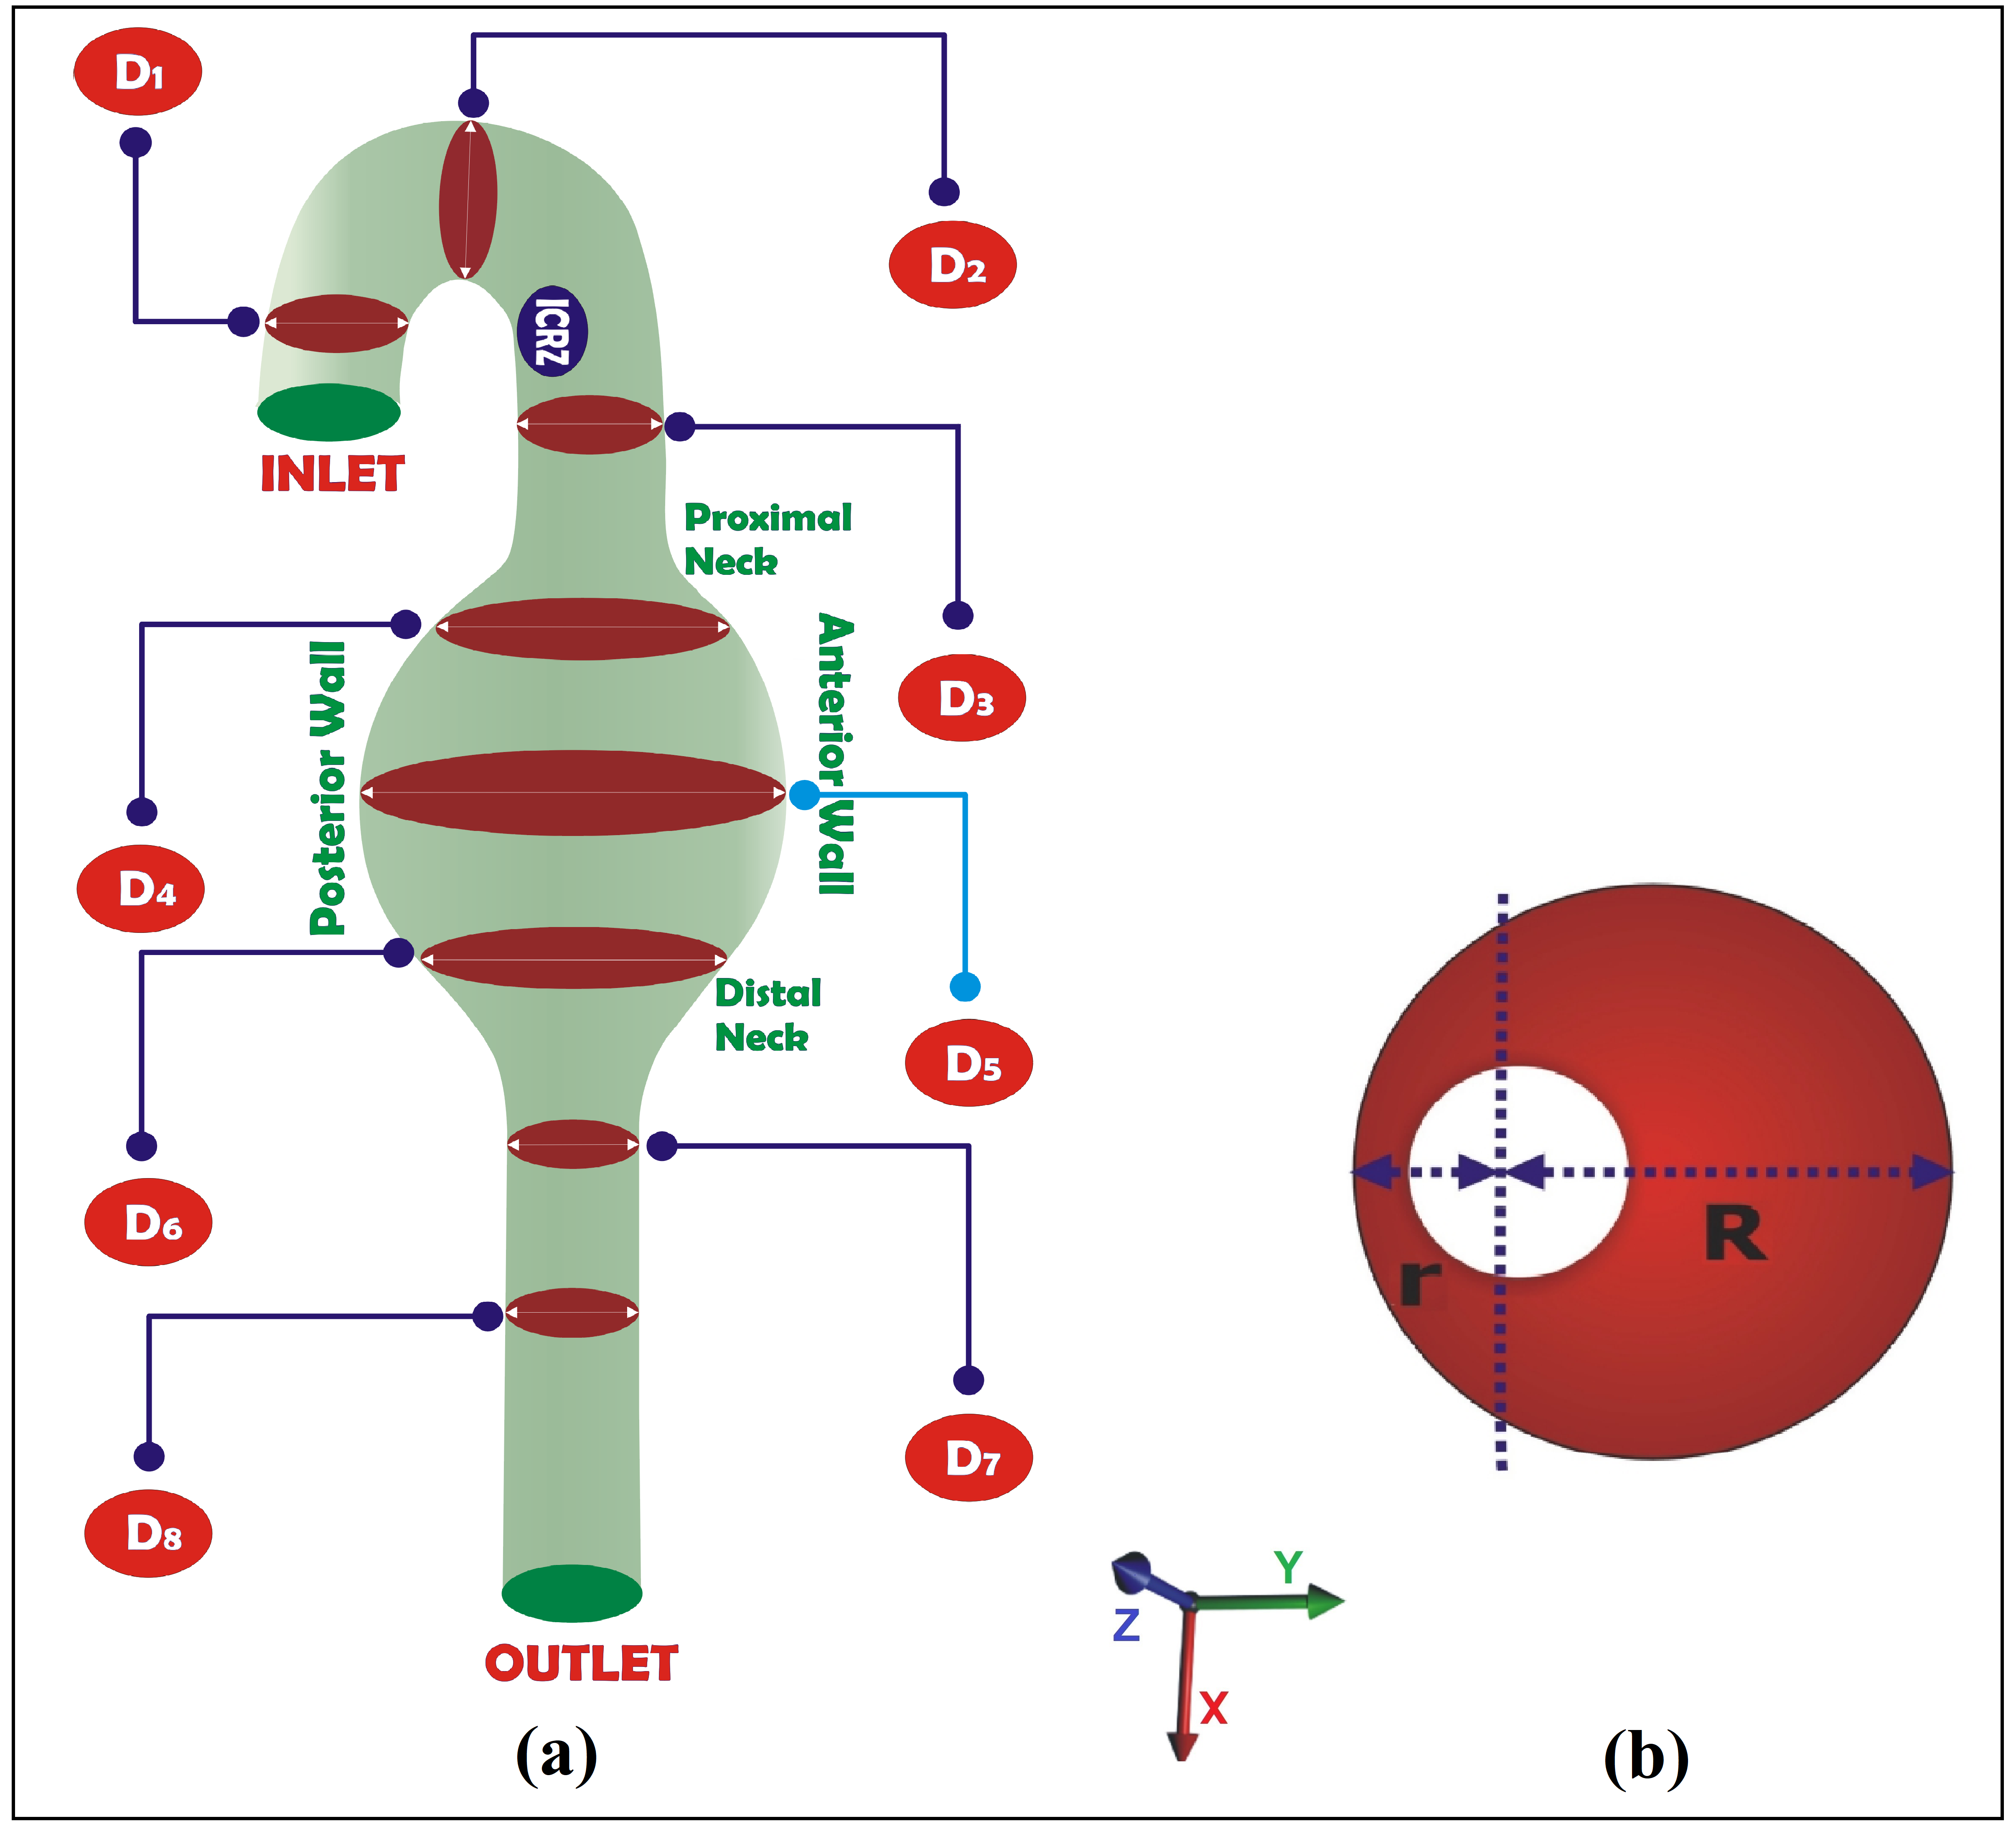
\includegraphics[width=1\textwidth, height=0.7\textheight]{Geometry.png}
         \caption{Visual depictions of (a) the three-dimensional geometry of the aneurysm and (b) the cross-sectional area of the aneurysm sac.}
         \label{fig:diagram}
     \end{figure}

     
\hspace*{\parindent} 

\subsection{\label{sec:governing_equations}Blood flow modeling and boundary conditions} 
\subsubsection{Governing equations and turbulence modeling}

The incompressible Navier--Stokes equations, which govern blood flow, are given by \cite{navier1823memoire, stokes2007theories}:
\begin{align}
    \nabla \cdot \mathbf{v} &= 0, \label{eq:cont}\\
    \rho \left( \frac{\partial \mathbf{v}}{\partial t} + (\mathbf{v} \cdot \nabla) \mathbf{v} \right) &= -\nabla p + \mu \nabla^2 \mathbf{v}, \label{eq:ns}
\end{align}
where \(\rho\) is the fluid density, \(\mathbf{v}\) the velocity vector, \(p\) the pressure, and \(\mu\) the dynamic viscosity.

For the unsteady Reynolds-averaged calculation, the instantaneous velocity will be decomposed as $\mathbf v=\mathbf V+\mathbf v'$ with $\overline{\mathbf v'}=0$, where $\mathbf V$ is the mean velocity. The Reynolds stress is closed by the Boussinesq eddy-viscosity approximation,
\begin{equation}
-\rho\overline{v_i'v_j'}=\mu_t\left(\partial_j V_i+\partial_i V_j\right)-\frac{2}{3}\rho k\delta_{ij},
\label{eq:boussinesq}
\end{equation}
where $k=\tfrac12\overline{v_i'v_i'}$ is \TKE per unit mass (m$^2$~s$^{-2}$), $\mu_t$ is dynamic eddy viscosity, and $\delta_{ij}$ is the Kronecker delta. With Eq.~\eqref{eq:boussinesq}, the Reynolds-averaged momentum equation solved for the mean velocity and pressure $P$ is
\begin{equation}
\rho\left(\frac{\partial\mathbf V}{\partial t}+(\mathbf V\cdot\nabla)\mathbf V\right)=-\nabla P+\nabla\cdot\left[(\mu+\mu_t)\left(\nabla\mathbf V+\nabla\mathbf V^{T}\right)\right]-\frac{2}{3}\nabla(\rho k),
\label{eq:urans}
\end{equation}
with $\nabla\cdot\mathbf V=0$.

\subsubsection{\texorpdfstring{\SSTcap \(k\)--\(\omega\) transition model}{SST k-omega transition model}}

The \SST \(k\)--\(\omega\) transition model was employed to account for the possible transition from laminar to turbulent flow and to capture the complex flow features associated with curvature, flow separation, and recirculation in the descending thoracic aorta. The model combines the near-wall formulation of the \(k\)--\(\omega\) model with the free-stream behavior of the \(k\)--\(\epsilon\) formulation through appropriate blending functions.

The turbulent eddy viscosity is calculated as
\begin{equation}
    \mu_t =
    \frac{a_1 \rho k}
    {\max(a_1\omega,\;SF_2)},
    \label{eq:mutt}
\end{equation}
where \(k\) is the \TKE, \(\omega\) is the specific dissipation rate, \(S\) is the magnitude of the strain-rate tensor, and \(F_2\) is the second blending function.

The transport equations for \TKE and specific dissipation rate are given by
\begin{equation}
\frac{\partial(\rho k)}{\partial t}
+\nabla\cdot(\rho k\mathbf{V})
=
\nabla\cdot
\left[
\left(\mu+\frac{\mu_t}{\sigma_k}\right)\nabla k
\right]
+P_k-D_k,
\label{eq:keqn}
\end{equation}

\begin{equation}
\frac{\partial(\rho\omega)}{\partial t}
+\nabla\cdot(\rho\omega\mathbf{V})
=
\nabla\cdot
\left[
\left(\mu+\frac{\mu_t}{\sigma_\omega}\right)\nabla\omega
\right]
+P_\omega-D_\omega
+
2(1-F_1)\rho\sigma_{\omega2}
\frac{1}{\omega}
\frac{\partial k}{\partial x_j}
\frac{\partial\omega}{\partial x_j}.
\label{eq:omegaeqn}
\end{equation}

Unlike the standard \SST \(k\)--\(\omega\) model, the transition formulation additionally solves two transport equations: one for the intermittency \(\gamma\), which varies from zero in laminar regions to unity in fully turbulent regions, and another for the transition momentum-thickness Reynolds number \(\widetilde{Re}_\theta\). These variables enable the model to predict the onset and development of boundary-layer transition based on the local flow conditions.

The blending functions \(F_1\) and \(F_2\) regulate the transition between the \(k\)--\(\omega\) and \(k\)--\(\epsilon\) formulations. \(F_1\) provides the appropriate near-wall blending, whereas \(F_2\) limits the eddy viscosity in regions where strain-rate effects become important. The distance to the nearest wall is denoted by \(y\). Thus, the \SST \(k\)--\(\omega\) transition model combines the strong near-wall behavior of the \(k\)--\(\omega\) formulation with the reduced free-stream sensitivity of the \(k\)--\(\epsilon\) formulation in the outer region of the boundary layer, while the additional intermittency and transition-Reynolds-number equations allow laminar--turbulent transition to be represented.




\subsubsection{Boundary conditions}
The pulsatile flow rate at the inlet is used in order to replicate the pulsatile nature of the blood flow in the human body. The inlet profile is expressed as:

\begin{equation}
Q(t)=
\begin{cases}
Q_0\,\sin\!\left(\dfrac{\pi\,(t-nT)}{0.35}\right)+0.05\,Q_0,
& nT \le t \le nT+0.35, \\[6pt]
0.05\,Q_0,
& nT+0.35 < t \le (n+1)T.
\end{cases}
\end{equation}


Similarly, the pulsatile outlet pressure is used at the outlet and is

\begin{equation}
P(t) =
\begin{cases} 
P_\mathrm{min} + \left(P_\mathrm{max} - P_\mathrm{min}\right) \, \sin\left(\dfrac{\pi \, (t - \, n \, T)}{0.35}\right), & nT \le t \le nT+0.35, \\
P_\mathrm{min}, & nT+0.35 < t \le (n+1)T.
\end{cases}
\end{equation}

Here $P_{\mathrm{min}}=80$~mmHg, $P_{\mathrm{max}}=120$~mmHg, $n=0,1,2,3$ indexes cardiac cycles, $T=0.8$~s, and $Q_0=2.39\times10^{-4}$~m$^3$~s$^{-1}$ is the sinusoidal amplitude. Because of the $0.05Q_0$ offset, the actual peak of the prescribed inlet flow rate is $1.05Q_0$.

{The inlet flow-rate and outlet pressure profiles that these two equations define are shown in Figure~\ref{fig:profiles}.}

\begin{figure}[!htb]
\centering
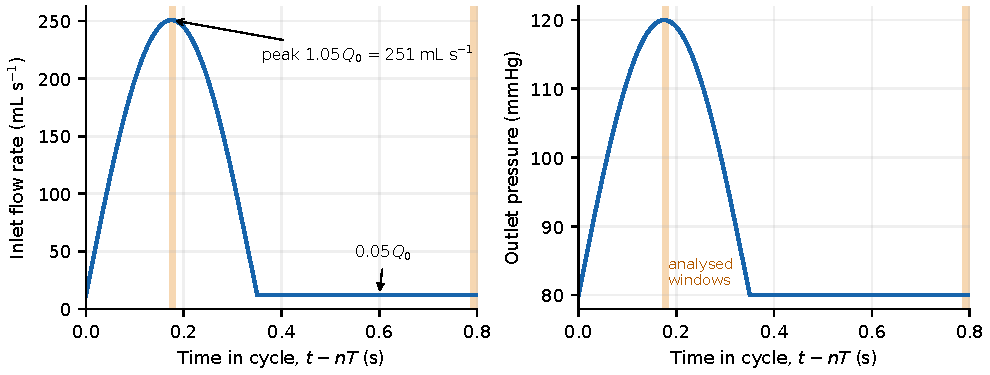
\includegraphics[width=\textwidth]{bc_profiles.pdf}
\caption{Prescribed inlet flow rate (left) and outlet pressure (right) over one cardiac cycle.}
\label{fig:profiles}
\end{figure}

A no-slip condition was imposed at the wall.



\subsubsection{\label{sec:Hemodynamics Parameters}Hemodynamic parameters}

\hspace*{\parindent} \WSScap  denotes the tangential force per unit area applied by blood flow against the vessel wall. The \WSS for vessels \cite{potters2015volumetric} can be calculated using the formula:

\begin{align}
    \tau_w = \mu \left. \frac{\partial {u_t}}{\partial n} \right|_{n=0},
\end{align}

where \(\mu\) is the blood viscosity, \(\frac{\partial {u_t}}{\partial n}\) is the {tangential velocity gradient} in the direction \(n\) normal to the wall, and {\(u_t\) is the local tangential velocity component at the wall}.

The cycle-averaged magnitude of \WSS was computed on the aneurysm wall~\cite{morbiducci2010outflow,turk2021characterization}:
\begin{equation}
\text{\TAWSScap} = \frac{1}{T} \int_{0}^{T} \left| \mathbf{WSS}(\mathbf{s},t) \right| \, dt,
\end{equation}
where $T$ is the duration of one cardiac cycle and $\mathbf{s}$ denotes a point on the vessel wall. \TAWSS  represents the magnitude of the \WSS vector averaged over time.

\TKEcap per unit mass, $k=\tfrac12\overline{v_i'v_i'}$, was used to summarize the modeled velocity fluctuations in the sac. It is a scalar quantity with units of m$^2$~s$^{-2}$, rather than the fluctuating velocity components themselves.

Speed and \TKE were also summarized at eight cross-sectional planes (D1--D8) to compare their variation along the vessel with local diameter.


\MPScap was evaluated on the inner wall surface to describe tensile loading in the structural model. It is the largest principal value of the local stress tensor. Elevated \MPS identifies modeled stress concentrations; predicting failure would additionally require local tissue-strength data, which were not available.

\subsubsection{\label{CFD Simulation}\texorpdfstring{\CFDcap}{CFD} simulation}ANSYS Fluent, a commercial finite-volume solver with a pressure-based formulation, was used to solve the governing equations for mass and momentum conservation. Blood was modeled as an incompressible Newtonian fluid with density \(\rho = 1050\,\mathrm{kg\,m^{-3}}\) and dynamic viscosity \(\mu = 3.5 \times 10^{-3}\,\mathrm{Pa\,s}\).


% AUTHOR CHECK: non-monotonic refinement and assumed p=2 do not establish an asymptotic convergence regime; add transient/multi-endpoint checks.
The spatial convergence of the steady flow results was checked by performing a mesh refinement study. Prescribed flow rate was \(2.39 \times 10^{-4} \, \mathrm{m^3/s}\) and the \SST \(k\)-\(\omega\) turbulence model was used. Four different meshes (2.9~mm to 0.8~mm) were used in the testing as shown in (Table~\ref{tab:mesh_study}). The relative change, Richardson-extrapolated value and \GCI were computed between each mesh and the immediately finer mesh. The assumed second order convergence rate, $p=2$ was used in conjunction with Roache's conservative safety factor, $F_s=3.0$ for the evaluation of the \GCI. The two first refinements had relatively high \GCI values, which means that the coarser meshes were not in the range of mesh independent solution. For comparison, refinement from 1.3~mm to 0.8~mm changed the maximum aneurysmal \WSS by only 0.89\%, was Richardson extrapolated to 66.83~Pa, and had a fine-grid \GCI value of 1.63\%. Therefore, the 0.8~mm mesh was selected for the final simulations.

\begin{table}[ht!]
\centering
\setlength{\tabcolsep}{3.5pt}
\caption{Reported steady-flow fluid-mesh refinement for maximum aneurysmal \WSS. The extrapolation assumes second-order convergence.}
\label{tab:mesh_study}
\setlength{\tabcolsep}{7pt}
\begin{tabular}{cccccc}
\toprule
Element & Number of & Maximum & Relative & Richardson- & GCI$_{\rm fine}$ \\
size & elements & aneurysm & change & extrapolated & (\%) \\
(mm) & & \WSS (Pa) & (\%) & \WSS (Pa) & \\
\midrule
2.9 & 62\,261    & 47.8 & --    & --    & -- \\
1.9 & 196\,142   & 55.4 & 13.72 & 61.12 & 30.95 \\
1.3 & 578\,040   & 67.8 & 18.29 & 78.71 & 48.29 \\
0.8 & 1\,475\,430 & 67.2 & 0.89  & 66.83 & 1.63 \\
\bottomrule
\end{tabular}
\end{table}


The temporal convergence was evaluated for three different time step sizes: 0.01~s, 0.001~s, and 0.0005~s. The difference between the two smaller time steps was small, less than 2\%, and there was very good agreement in the \WSS waveforms. The time step was chosen as 0.001~s, which was found to be adequate in terms of both the level of temporal resolution and computational efficiency.

To eliminate initial transient effects and ensure a periodic steady state, the simulations were run for four consecutive cardiac cycles (\(n = 0,1,2,3\)). The percentage difference in \WSS between the third and fourth cycles was negligible (mean \(< 0.4\%\)), confirming that a periodic steady state had been reached. Accordingly, snapshots from the third cardiac cycle were used for the instantaneous flow comparisons. The exact averaging cycle of the retained \TAWSS export requires separate confirmation.



\subsubsection{Pressure-loaded structural model}

The arterial wall was modeled using ANSYS mechanical and considered as a nearly incompressible, isotropic hyperelastic material using the second-order Yeoh strain energy potential. The strain energy density function is
\begin{equation}
W = C_{10}(\bar{I}_1 - 3) + C_{20}(\bar{I}_1 - 3)^2,
\label{eq:yeoh}
\end{equation}
% AUTHOR CHECK: confirm material constants by group, prestress/reference state, external pressure and solid-mesh convergence.
where \(W\) is the strain energy density, \(\bar{I}_1\) is the first deviatoric strain invariant, and \(C_{10}\) and \(C_{20}\) are material constants. The material constants were set to \(C_{10} = 98.8~\text{kPa}\) and \(C_{20} = 779.1~\text{kPa}\) \cite{zhu2025combined}. The incompressibility parameter \(D_1\) was specified as \(2.04 \times 10^{-4}~\text{kPa}^{-1}\), corresponding to a Poisson's ratio of \(\nu = 0.49\). A uniform wall thickness of 2.0~mm was assumed for all models, consistent with previous idealized \FSI studies of thoracic \AANs, and the arterial wall density was set to 1120~kg/m\(^3\).

Both ends of the structural domain were fixed. Fluid pressure was transferred to the inner wall surface in ANSYS Mechanical (Figure~\ref{fig:Flowchart}). All quantitative flow and reconstruction results use the rigid-wall fluid solution (Section~\ref{sec:exports}). The retained coupling records are insufficient to establish a bidirectional moving-wall calculation; the structural results are therefore interpreted as pressure-loaded wall-stress fields.



\begin{figure}[!ht]
  \centering
  \definecolor{cIn}{HTML}{1F6FB2}
  \definecolor{cNet}{HTML}{0E8C84}
  \definecolor{cData}{HTML}{C0392B}
  \definecolor{cPhys}{HTML}{B07A12}
  \definecolor{cPost}{HTML}{2E7D32}
  \definecolor{cOpt}{HTML}{555555}
  \resizebox{\textwidth}{!}{%
  \begin{tikzpicture}[
      font=\small,
      >={Stealth[length=2.2mm]},
      box/.style={rounded corners=2pt, draw=#1!70, line width=0.6pt, fill=#1!7,
                  align=center, inner sep=4pt, text=black, minimum width=52mm, minimum height=9mm},
      dec/.style={diamond, aspect=2.2, draw=cOpt!70, fill=cOpt!7, line width=0.6pt, inner sep=1.5pt, font=\small},
      arr/.style={->, draw=black!65, line width=0.7pt},
      lab/.style={font=\footnotesize, text=black!70},
      ilab/.style={font=\footnotesize\itshape, text=black!60},
    ]

    % ---------------------------------------------------------
    % Top: geometry
    % ---------------------------------------------------------
    \node[box=cOpt, minimum width=60mm] (geo) {\textbf{Geometry}: Twelve idealized models};

    % ---------------------------------------------------------
    % Left column: fluid
    % ---------------------------------------------------------
    \node[box=cIn, below left=8mm and -14mm of geo] (fl) {\textbf{Fluid (blood)}: ANSYS Fluent};
    \node[box=cIn, below=4mm of fl] (fmesh) {Mesh generation};
    \node[box=cIn, below=4mm of fmesh, align=center] (fset) {%
        Fluid properties and boundary conditions.\\
        Discretization method and convergence setup.};
    \node[dec, below=5mm of fset] (conv) {converged?};
    \node[box=cIn, below=6mm of conv] (fres) {Results};

    \draw[arr] (fl) -- (fmesh);
    \draw[arr] (fmesh) -- (fset);
    \draw[arr] (fset) -- (conv);
    \draw[arr] (conv) -- node[lab, right]{yes} (fres);

    \coordinate (loopx) at ($(fset.west)+(-5mm,0)$);
    \draw[arr] (conv.west) -- node[lab, above]{no} (conv.west -| loopx) |- (fset.west);

    % ---------------------------------------------------------
    % Right column: solid
    % ---------------------------------------------------------
    \node[box=cPost, below right=8mm and -14mm of geo] (so) {\textbf{Solid (wall)}: ANSYS Mechanical};
    \node[box=cPost, below=4mm of so] (smesh) {Mesh generation};
    \node[box=cPost, below=4mm of smesh, align=center] (sset) {%
        Wall properties and boundary conditions.};
    \node[box=cPost, below=4mm of sset] (sa) {Stress analysis};
    \node[box=cPost, below=4mm of sa] (sres) {Results};
    \node[box=cPost, below=4mm of sres] (end) {End};

    \draw[arr] (so) -- (smesh);
    \draw[arr] (smesh) -- (sset);
    \draw[arr] (sset) -- (sa);
    \draw[arr] (sa) -- (sres);
    \draw[arr] (sres) -- (end);

    % ---------------------------------------------------------
    % Links from geometry to both columns
    % ---------------------------------------------------------
    \draw[arr] (geo.south) -- ++(0,-3mm) -| (fl.north);
    \draw[arr] (geo.south) -- ++(0,-3mm) -| (so.north);

    % ---------------------------------------------------------
    % Wall-pressure transfer from fluid to solid
    % ---------------------------------------------------------
    \coordinate (cpx) at ($(fset.east)!0.5!(fset.east -| sa.west)$);
    \draw[arr, draw=cPhys!90, line width=0.9pt]
          (fres.east) -- (fres.east -| cpx) -- (cpx |- sa.west) -- (sa.west);
    \node[lab, text=cPhys!90!black, rotate=90, anchor=north, inner sep=1pt]
          at ($(fres.east -| cpx)!0.5!(cpx |- sa.west)$) {wall pressure};

  \end{tikzpicture}%
  }
  \caption{\CFDcap and structural workflow. The fluid problem is solved in ANSYS Fluent, and the wall pressure is transferred to the structural model in ANSYS Mechanical.}
  \label{fig:Flowchart}
\end{figure}



\section{Sparse-velocity reconstruction methods}
\label{sec:reconstruction_methods}
\subsection{Exported flow fields, instants and regions}
\label{sec:exports}
All quantitative flow results in this paper, including the reconstruction study, use whole-domain exports of the rigid-wall \CFD solutions rather than the structural calculation. For each case the exports contain every fluid node (468\,000--603\,000 interior nodes and 34\,600--41\,400 wall nodes) with velocity, static pressure, eddy viscosity $\mu_t$, $k$ and $\omega$, together with the \WSS vector on the wall nodes and the inlet and outlet faces. The mesh and node ordering are identical across the snapshots of a case, so differences between snapshots are exact nodal differences. No cell volumes, face areas or connectivity were exported, and all averages are therefore node-weighted. The near-wall node spacing differs between the two groups of models. In the aneurysmal models the interior node nearest each wall node lies a median 0.03--0.04~mm from the wall in the aneurysm zone but 0.58~mm on the rest of the wall, including the bend, whereas in the controls it lies 0.04~mm from the wall everywhere. Near-wall refinement in the aneurysmal models is therefore confined to the aneurysm zone, and quantities outside that zone, including comparisons with the controls there, depend on near-wall resolution as well as on geometry.

Snapshots exist for every case at 1.780~s and at 2.390 and 2.400~s, and for all cases except Case~2 at 1.775~s; Case~2 instead has a snapshot at 1.788~s, which completes its systolic window. Peak inflow occurs at 1.775~s, $0.175$~s into the third cycle, so 1.780~s is 5~ms after the peak, and 2.400~s is the end of the diastolic plateau of the third cycle. We use 1.780~s and 2.400~s as common systolic and diastolic instants and refer to them below as the systolic and diastolic phases. All exported fields were post-processed and plotted with Python scripts (NumPy, SciPy and Matplotlib). The earlier case-specific image exports were taken at different near-systolic times (1.775--1.815~s), and they are used only as qualitative illustrations.

Two regions are used throughout. The \emph{aneurysm zone} is the wall zone exported as the dilation for each aneurysmal case, which spans the sac and its necks. For comparisons that include the controls, the \emph{dilation segment} is the axial extent of the aneurysm zone of the axisymmetric case with the same inlet diameter, restricted to the descending branch, so that each control is evaluated over the corresponding stretch of undilated vessel. Within the straight descending segment the global $x$ axis coincides with the local downstream direction, which makes a negative $x$ velocity a meaningful indicator of reversed flow there, unlike in the curved inlet region.


\subsection{Task and information available to each method}
\label{sec:task}
Each reconstruction problem concerns one geometry and one short window of two snapshots. The systolic window is 1.775--1.780~s, with the target at 1.780~s, except for Case~2, which has no 1.775~s export and uses 1.780--1.788~s with the same target. The diastolic window is 2.390--2.400~s, with the target at 2.400~s. Given velocity at a sparse set of interior nodes at both window times, a method must recover velocity at all other interior nodes, the gauge pressure in the interior and the \WSS magnitude on the aneurysm zone at the target time. The geometry is known, so the task is reconstruction within a given anatomy rather than prediction for a new one.

Table~\ref{tab:information} lists what each method may use. Geometry comprises the coordinates of the interior nodes without their field values, the wall nodes with inward normals, and the inlet and outlet faces. Boundary information comprises the prescribed inlet velocity and the mean outlet pressure at each window time. Pressure, \WSS and velocity at unobserved nodes are never used for fitting or selection. We examine two viscosity settings. The first supplies the \CFD eddy-viscosity field $\mu_t$ and its spatial gradient, so the momentum balance uses $\mu+\mu_t$. We call this the \emph{oracle} setting because it gives the reconstruction access to closure information from the reference simulation. The second uses only the prescribed blood viscosity, $\mu=3.5\times10^{-3}$~Pa~s, with $\mu_t=0$; this is the \emph{molecular-viscosity} setting. The \CFD eddy viscosity is not measured by the sparse velocity observations. Results that use it are therefore conditional on that additional information.

\begin{table}[htbp]
\centering
\small
\caption{Information used by each method. All methods receive the same observation nodes at both window times and are scored through the same post-processing.}
\label{tab:information}
\setlength{\tabcolsep}{4pt}
\begin{tabular}{p{4.3cm}ccccc}
\toprule
Information & Linear & \RBF & \shortstack{Data\\field} & \shortstack{Continuity\\field} & \shortstack{Momentum\\\PINN} \\
\midrule
Sparse velocity at two times & \checkmark & \checkmark & \checkmark & \checkmark & \checkmark \\
Wall no-slip and inlet velocity & \checkmark & \checkmark & \checkmark & \checkmark & \checkmark \\
Outlet pressure datum & post-proc. & post-proc. & \checkmark & \checkmark & \checkmark \\
Interior node coordinates (no values) & -- & -- & -- & \checkmark & \checkmark \\
Continuity in the fit & -- & -- & -- & \checkmark & \checkmark \\
Momentum balance in the fit & -- & -- & -- & -- & \checkmark \\
\CFDcap $\mu_t$ (oracle setting) & post-proc. & post-proc. & post-proc. & post-proc. & fit + post-proc. \\
\bottomrule
\end{tabular}
\end{table}

\subsection{Observation design}
\label{sec:observations}
Velocity is observed at the interior nodes nearest to the points of a uniform Cartesian grid with spacing $\Delta$ and a random offset, keeping only grid points with an interior node within $\Delta/2$. The same nodes are observed at both window times. Sampling on a grid rather than on mesh nodes avoids oversampling the refined near-wall layers. Each grid point is, however, snapped to a mesh node, so observations next to the wall fall on the prism layers. At $\Delta=2.5$~mm, 5.6--8.5\% of the observed nodes of Cases~2--8 lie within 0.25~mm of the wall and 26--30\% within 1~mm, the closest at 0.03~mm, whereas a 2.5~mm imaging voxel would return an average over its volume. The design is therefore point sampling on a grid rather than voxel sampling. Every method receives the same observations, so the comparison between methods is not affected, but the absolute \WSS errors are optimistic relative to imaging data; Section~\ref{sec:nearwall} quantifies this by removing the near-wall observations. The primary spacing $\Delta=2.5$~mm observes 1.27--1.36\% of the interior nodes per time (5\,970--8\,205 nodes), and the secondary spacings of 1.5 and 4.0~mm observe 5.4--5.8\% and 0.34--0.37\%. The observed values are noise-free \CFD values at mesh nodes. The neural fields withhold a random 10\% of sampled nodes from fitting for model selection and monitoring. The fixed interpolation comparators use all sampled observations; the tuned comparators use the holdout for selection and then refit using all observations. Thus the sampled observation pool is shared, but the final fitting subsets differ. Each draw $s$ fixes both the grid offset and the network initialization, draws are paired across methods, and the observed node indices are stored.


\subsection{Space-time neural fields and physics constraints}
\label{sec:field}
We use a space-time neural field to represent each short flow window. The confirmation method is a continuity-constrained field followed by physics-based post-processing, in which the network reconstructs velocity and separate calculations recover pressure and \WSS. We refer to this method as the continuity field. Its divergence penalty is a physical constraint, but it does not enforce the momentum balance during fitting. We use the term \emph{momentum \PINN} for the separate arms, tested only on the two development geometries, that also penalize the momentum residual. 

All neural arms share the same architecture, which maps position and time to velocity and pressure, $(\mathbf x,t)\mapsto(\mathbf u_\theta,p_\theta)$. Coordinates are scaled as $\mathbf x_s=(\mathbf x-\mathbf x_c)/L$, where $\mathbf x_c$ is the centroid of the interior nodes and $L$ is half the largest extent of the domain, and time is mapped to $t_s\in[-1,1]$ across the window. Velocity is scaled by $U$, the 99.5th percentile of training-observation speed at the target time, and pressure by $\rho U^2$. The input is $[\sin(2\pi\mathbf B^{\mathsf T}\mathbf x_s),\cos(2\pi\mathbf B^{\mathsf T}\mathbf x_s),\mathbf x_s,t_s]$, where $\mathbf B\in\mathbb R^{3\times64}$ holds Gaussian Fourier features with a \SD of 2~\cite{tancik2020fourier}, followed by six fully connected layers of width 256 with SiLU activations and a linear output of four scaled quantities (about 360\,000 parameters) (Figure~\ref{fig:network}).

\begin{figure}[!t]
  \centering
  \definecolor{cIn}{HTML}{1F6FB2}
  \definecolor{cEnc}{HTML}{6A4C93}
  \definecolor{cNet}{HTML}{0E8C84}
  \definecolor{cData}{HTML}{C0392B}
  \definecolor{cPhys}{HTML}{B07A12}
  \definecolor{cBC}{HTML}{2E7D32}
  \definecolor{cOpt}{HTML}{555555}
  \resizebox{\textwidth}{!}{%
  \begin{tikzpicture}[
      font=\small,
      >={Stealth[length=2.2mm]},
      box/.style={rounded corners=2pt, draw=#1!70, line width=0.6pt, fill=#1!7,
                  align=center, inner sep=3.5pt, text=black},
      box/.default=black,
      inp/.style={box=cIn,  minimum width=24mm, minimum height=9mm},
      enc/.style={box=cEnc, minimum width=30mm, minimum height=10mm},
      cat/.style={draw=black!55, fill=black!6, circle, inner sep=1.5pt, minimum size=13mm, align=center},
      outn/.style={circle, draw=#1!75, fill=#1!16, line width=0.6pt, minimum size=7.5mm,
                  inner sep=0pt, font=\footnotesize},
      loss/.style={box=#1, minimum width=40mm, minimum height=12mm},
      opt/.style={box=cOpt, minimum width=36mm, minimum height=10mm},
      neuron/.style={circle, draw=cNet!70, fill=cNet!12, minimum size=3.4mm, inner sep=0pt},
      edge/.style={draw=cNet!35, line width=0.25pt},
      arr/.style={->, draw=black!65, line width=0.7pt},
      bus/.style={draw=black!60, line width=0.7pt},
      lab/.style={font=\footnotesize, text=black!70},
      ilab/.style={font=\footnotesize\itshape, text=black!60},
    ]
    \node[inp] (x) {$\mathbf{x}=(x,y,z)$};
    \node[inp, below=12mm of x] (t) {$t\in[t_o,t_\star]$};
    \node[lab, left=1mm of x] (lx) {position};
    \node[lab, left=1mm of t] (lt) {time};
    \node[enc, right=10mm of x] (fF) {Fourier features $\gamma(\mathbf{x}_s)$\\{\footnotesize 64 frequencies, $\sigma=2$}};
    \node[enc, right=10mm of t] (ts) {window scaling\\{\footnotesize $t_s\in[-1,1]$}};
    \coordinate (mid) at ($(fF.east)!0.5!(ts.east)$);
    \node[cat, right=9mm of mid] (cat) {\scriptsize concat\\[-1pt]\scriptsize $[\gamma,\mathbf{x}_s,t_s]$};
    \draw[arr] (x) -- (fF);
    \draw[arr] (t) -- (ts);
    \draw[arr] (fF.east) -- ([yshift= 2mm]cat.west);
    \draw[arr] (ts.east) -- ([yshift=-2mm]cat.west);

    \coordinate (netorg) at ($(cat.east)+(27mm,0)$);
    \begin{scope}[shift={(netorg)}]
      \node[rounded corners=3pt, draw=cNet!70, fill=white, minimum width=38mm, minimum height=27mm] (mlp) {};
      \foreach \i in {1,2,3}\node[neuron] (a\i) at (-15mm, {(\i-2)*6mm}) {};
      \foreach \i in {1,2,3,4}\node[neuron] (b\i) at (-5mm, {(\i-2.5)*5mm}) {};
      \foreach \i in {1,2,3,4}\node[neuron] (c\i) at (5mm,  {(\i-2.5)*5mm}) {};
      \node[neuron] (d1) at (15mm,0) {};
      \foreach \i in {1,2,3}\foreach \j in {1,2,3,4}\draw[edge] (a\i)--(b\j);
      \foreach \i in {1,2,3,4}\foreach \j in {1,2,3,4}\draw[edge] (b\i)--(c\j);
      \foreach \i in {1,2,3,4}\draw[edge] (c\i)--(d1);
    \end{scope}
    \node[ilab, text=cNet!80, below=1.5mm of mlp] (mlplab) {6 layers $\times$ 256 units, SiLU};
    \draw[arr] (cat.east) -- (a2);

    \node[outn=cIn, right=15mm of mlp, yshift=11.5mm] (ou) {$u$};
    \node[outn=cIn, below=2.2mm of ou] (ov) {$v$};
    \node[outn=cIn, below=2.2mm of ov] (ow) {$w$};
    \node[outn=cPhys, below=2.2mm of ow] (op) {$p$};
    \foreach \o in {ou,ov,ow,op}{\draw[arr] (d1) -- (\o);}
    \draw[decorate, decoration={brace, amplitude=3pt, raise=1pt}, draw=black!50, line width=0.5pt]
      ($(ou.east)+(1.5mm,0)$) -- ($(ow.east)+(1.5mm,0)$);
    \node[lab, anchor=west] (lvel) at ($(ov.east)+(5.5mm,0)$) {velocity};
    \node[lab, anchor=west] (lpre) at (lvel.west |- op) {pressure};

    \begin{scope}[on background layer]
      \node[rounded corners=4pt, draw=black!40, fill=black!1.5,
            fit=(lx)(lt)(x)(t)(fF)(ts)(cat)(mlp)(mlplab)(ou)(op)(lvel)(lpre), inner sep=5mm] (net) {};
    \end{scope}
    \node[ilab, anchor=south west, text=black!65] at ($(net.north west)+(1.5mm,0.8mm)$)
         {Network $f_\theta(\mathbf{x},t)$, fitted separately for each case and window};

    \node[loss=cPhys] (phys) at ($(net.south)+(0,-16mm)$)
         {\textbf{Physics}, weight $w=0.01$\\continuity $\nabla\!\cdot\mathbf{u}$\\{\footnotesize\color{black!60}momentum \PINNs: + momentum residual}};
    \node[loss=cData, left=10mm of phys] (data)
         {\textbf{Data}\\$\mathbf{u}$ at observed nodes, $t_o$ and $t_\star$};
    \node[loss=cBC, right=10mm of phys] (bc)
         {\textbf{Boundary}\\no-slip, inlet $\mathbf{u}$, outlet datum};
    \coordinate (busL) at ($(net.south)+(0,-6mm)$);
    \draw[bus] (net.south) -- (busL);
    \node[ilab, anchor=south west, text=black!70] at ($(net.south)+(1.8mm,-1mm)$) {predictions};
    \draw[bus] (busL) -| (data.north);
    \draw[arr] (busL) -- (phys.north);
    \draw[bus] (busL) -| (bc.north);
    \draw[arr] ($(data.north)+(0,2mm)$)--(data.north);
    \draw[arr] ($(bc.north)+(0,2mm)$)--(bc.north);

    \node[opt, minimum width=48mm] (sum) at ($(phys.south)+(0,-11mm)$) {$\mathcal L=\mathcal L_{\rm data}+\mathcal L_{\rm bc}+w\,\mathcal L_{\rm phys}$};
    \node[opt, below=6mm of sum] (adam) {Adam, lr $10^{-3}\!\to\!10^{-5}$ (cosine),\\20\,000 steps, gradient clipping};
    \draw[arr] (data.south) |- (sum.west);
    \draw[arr] (phys.south) -- (sum.north);
    \draw[arr] (bc.south) |- (sum.east);
    \draw[arr] (sum.south) -- (adam.north);
    \coordinate (fbmid) at ([xshift=7mm]net.east);
    \coordinate (fbbot) at (fbmid |- adam.east);
    \draw[arr, dashed, draw=black!55] (adam.east) -- (fbbot)
       -- node[lab, pos=0.55, right]{$\nabla_\theta$} (fbmid) -- (net.east);
  \end{tikzpicture}%
  }
  \caption{Space-time neural field. Fourier-encoded position and scaled time pass through a fully connected network to velocity and pressure, fitted to the observed velocity and the boundary conditions. The continuity arm adds a divergence penalty; the momentum residual (gray) was used only by the momentum \PINNs tested on the two development geometries.}
  \label{fig:network}
\end{figure}


The loss combines data and boundary terms with an optional physics term,
\begin{equation}
\mathcal L=\mathcal L_{\rm obs}+\mathcal L_{\rm wall}+\mathcal L_{\rm in}+\mathcal L_{\rm out}+w\,\mathcal L_{\rm phys},
\label{eq:loss}
\end{equation}
where $\mathcal L_{\rm obs}$ is the mean squared velocity misfit at the observed nodes at both times, $\mathcal L_{\rm wall}$ penalizes velocity at wall nodes at random times in the window, $\mathcal L_{\rm in}$ penalizes the misfit to the prescribed inlet velocity at each window time, and $\mathcal L_{\rm out}$ penalizes the squared mean of $p_\theta$ on the outlet face, which fixes the pressure datum. Four arms differ only in $\mathcal L_{\rm phys}$. The \emph{data} arm has none. The \emph{continuity} arm uses the mean squared divergence $(\nabla\cdot\mathbf u_\theta)^2$ at interior nodes drawn at random times. The \emph{steady} and \emph{unsteady} momentum arms add the mean squared residual of
\begin{equation}
\rho\,\partial_t\mathbf u+\rho(\mathbf u\cdot\nabla)\mathbf u
+\nabla p-\nabla\cdot\left[(\mu+\mu_t)
(\nabla\mathbf u+\nabla\mathbf u^{\mathsf T})\right]=\mathbf 0,
\label{eq:momentum}
\end{equation}
% AUTHOR CHECK: verify the exported Fluent/CFD-Post pressure definition and isotropic turbulent-stress convention from the solver setup.
without the time term in the steady arm, with $\mu_t$ interpolated linearly in time between the two snapshots in the oracle setting and set to zero in the molecular setting. Derivatives are taken by automatic differentiation, and the variable-viscosity divergence retains the gradient of $\mu_t$. Equation~\eqref{eq:momentum} has no separate $2\rho k/3$ term because the exported \CFD pressure satisfies the momentum balance better without it (Section~\ref{sec:reference_results}), which is consistent with an effective-pressure convention but does not, by itself, verify the solver's exported pressure definition.

Each step draws 4096 observations, 4096 collocation nodes, 2048 wall nodes, 512 inlet nodes per time and 256 outlet nodes per time. Training uses Adam with a learning rate of $10^{-3}$, cosine decay to $10^{-5}$ over 20\,000 steps and gradient-norm clipping at 1. There is no early stopping, and the last iterate is scored. The physics weight $w$ was chosen for each arm from $\{0.01,0.1,1\}$ on Case~1 at systole by the error on the withheld observations and then frozen. That error increased with $w$ in every arm, so $w=0.01$ was used throughout. On one NVIDIA Quadro RTX 8000 shared with other jobs, a 20\,000-step fit took a median of 23~min for the continuity arm and 17~min for the data arm.

\subsection{Interpolation comparators}
\label{sec:interpolation}
The comparators interpolate the same observations, with zero velocity at the wall nodes and the prescribed inlet velocity added as sources, separately at each window time. \emph{Linear} interpolation uses the Delaunay triangulation of the sources, with the nearest source used outside its hull. \emph{\RBF} interpolation uses a local thin-plate-spline \RBF with a linear polynomial on the 64 nearest sources, with fallback neighborhoods of 128 and then 256 sources if the local system is singular. These settings were fixed before the development test and are the prespecified comparator. Two further comparators were added after the confirmatory verdict as robustness checks. The \emph{tuned \RBF} selects the kernel (thin-plate spline, cubic or quintic), the neighborhood size (32--256) and the smoothing parameter ($0$--$10^{-2}$) by the error on the withheld observations. The \emph{space-time \RBF} fits one interpolant over $(\mathbf x, c\,t)$ through both snapshots, with the time scale $c\in\{0,0.5,2,8\}$~m~s$^{-1}$, the kernel and the neighborhood size chosen on the same withheld observations.

\subsection{Shared post-processing}
\label{sec:postprocessing}
Every reconstruction, including the complete \CFD velocity used as a reference, is converted to pressure and \WSS by the same steps (Figure~\ref{fig:pipeline}). The reconstructed velocity is first sampled at the \CFD nodes. Spatial gradients are computed by weighted least squares on the 40 nearest nodes with inverse-square-distance weights, with zero velocity imposed at the wall nodes. The momentum balance then gives a target pressure gradient,
\begin{equation}
\mathbf f=-\rho\,\frac{\mathbf u(t_\star)-\mathbf u(t_o)}{t_\star-t_o}
-\rho(\mathbf u\cdot\nabla)\mathbf u
+\nabla\cdot\left[(\mu+\mu_t)(\nabla\mathbf u+\nabla\mathbf u^{\mathsf T})\right],
\label{eq:pressure_rhs}
\end{equation}
evaluated at the target time $t_\star$, where $t_o$ is the other window time. The gauge pressure is the least-squares solution of $\nabla_h p=\mathbf f$ on the interior nodes more than 1~mm from the wall, with the mean pressure over nodes beyond $x=0.130$~m set to zero, computed with LSQR. Near-wall nodes are excluded because the prism-layer stencils are poorly conditioned. Dropping the first term of Eq.~\eqref{eq:pressure_rhs} gives the steady form, and setting $\mu_t=0$ gives the molecular form. All four combinations are reported, and the unsteady form with oracle $\mu_t$ is the prespecified pressure endpoint. The steady form of Eq.~\eqref{eq:pressure_rhs} is the standard pressure-gradient route of velocity-based relative-pressure estimation~\cite{bertoglio2018relative}.

\WSScap is estimated at each aneurysm-zone wall node $\mathbf x_w$ with inward unit normal $\mathbf n$ from the tangential velocity $\mathbf u_t$ at two distances inside the lumen,
\begin{equation}
\boldsymbol\tau_w\approx\mu\,\frac{4\,\mathbf u_t(\mathbf x_w+h\mathbf n)-\mathbf u_t(\mathbf x_w+2h\mathbf n)}{2h},
\label{eq:wss_estimate}
\end{equation}
which is second-order accurate for a no-slip wall, with $\mathbf u_t$ obtained by linear interpolation of the nodal velocity. The prespecified distance is $h=0.25$~mm, and results at 0.1 and 0.5~mm are reported only as an oracle sensitivity. In the aneurysm zone the interior node nearest the wall lies a median 0.03--0.04~mm from it, so Eq.~\eqref{eq:wss_estimate} is informative there. Outside the aneurysm zone that distance is 0.58~mm, and even the complete \CFD velocity reproduces the exported \WSS there only to a relative error of 0.46--0.68, so \WSS outside the aneurysm zone is not used as a target.


\begin{figure}[!t]
  \centering
  \definecolor{cIn}{HTML}{1F6FB2}
  \definecolor{cNet}{HTML}{0E8C84}
  \definecolor{cData}{HTML}{C0392B}
  \definecolor{cPhys}{HTML}{B07A12}
  \definecolor{cPost}{HTML}{2E7D32}
  \definecolor{cOpt}{HTML}{555555}
  % outline of an idealized aneurysmal segment, used by the pictograms below
  \def\vesselpath{(-1.1,0.22) -- (-0.45,0.22) .. controls (-0.25,0.62) and (0.25,0.62) .. (0.45,0.22)
    -- (1.1,0.22) -- (1.1,-0.22) -- (0.45,-0.22) .. controls (0.25,-0.62) and (-0.25,-0.62) .. (-0.45,-0.22)
    -- (-1.1,-0.22) -- cycle}
  \resizebox{\textwidth}{!}{%
  \begin{tikzpicture}[
      font=\small,
      >={Stealth[length=2.2mm]},
      card/.style={rounded corners=3pt, draw=#1!70, line width=0.6pt, fill=#1!6},
      ttl/.style={font=\small\bfseries, text=black, align=center},
      sub/.style={font=\footnotesize, text=black!72, align=center},
      arr/.style={->, draw=black!60, line width=0.7pt},
      ln/.style={draw=black!60, line width=0.7pt},
      step/.style={circle, fill=#1, text=white, font=\footnotesize\bfseries, inner sep=0pt, minimum size=4.8mm},
      steplab/.style={font=\small\bfseries, text=black!75, anchor=west},
      % ---------- pictograms ----------
      obsicon/.pic={
        \draw[cIn!70, line width=0.6pt, fill=white] \vesselpath;
        \foreach \x in {-0.9,-0.6,...,0.95}{\fill[cIn] (\x,0.1) circle (0.045); \fill[cIn] (\x,-0.1) circle (0.045);}
        \foreach \x in {-0.2,0.1}{\fill[cIn] (\x,0.36) circle (0.045); \fill[cIn] (\x,-0.36) circle (0.045);}
      },
      linicon/.pic={
        \draw[cOpt!80, line width=0.45pt, fill=cOpt!10]
          (0,0) -- (0.5,0.08) -- (0.22,0.45) -- cycle (0.5,0.08) -- (0.78,0.46) -- (0.22,0.45)
          (0,0) -- (-0.28,0.36) -- (0.22,0.45);
        \foreach \p in {(0,0),(0.5,0.08),(0.22,0.45),(0.78,0.46),(-0.28,0.36)}{\fill[cIn] \p circle (0.05);}
      },
      rbficon/.pic={
        \draw[cOpt!45, line width=0.4pt] (-0.45,0) -- (0.85,0);
        \draw[cOpt!85, line width=0.7pt, domain=-0.45:0.85, samples=50, smooth]
          plot (\x,{0.45*exp(-((\x+0.02)^2)/0.03)+0.28*exp(-((\x-0.45)^2)/0.02)});
        \fill[cIn] (-0.02,0.45) circle (0.05); \fill[cIn] (0.45,0.29) circle (0.05);
      },
      nnicon/.pic={
        \foreach \a in {-0.22,0,0.22}{\foreach \b in {-0.33,-0.11,0.11,0.33}{\draw[cNet!35, line width=0.3pt] (0,\a) -- (0.4,\b);}}
        \foreach \b in {-0.33,-0.11,0.11,0.33}{\draw[cNet!35, line width=0.3pt] (0.4,\b) -- (0.8,0.1); \draw[cNet!35, line width=0.3pt] (0.4,\b) -- (0.8,-0.1);}
        \foreach \a in {-0.22,0,0.22}{\fill[cNet] (0,\a) circle (0.05);}
        \foreach \b in {-0.33,-0.11,0.11,0.33}{\fill[cNet] (0.4,\b) circle (0.05);}
        \fill[cNet] (0.8,0.1) circle (0.05); \fill[cNet] (0.8,-0.1) circle (0.05);
      },
      velicon/.pic={
        \draw[cIn!70, line width=0.6pt, fill=white] \vesselpath;
        \foreach \x in {-0.95,-0.65,0.45,0.75}{\draw[->, >={Stealth[length=0.8mm]}, cIn, line width=0.45pt] (\x,0) -- ++(0.24,0);}
        \draw[->, >={Stealth[length=0.8mm]}, cIn, line width=0.45pt] (-0.3,0) -- ++(0.55,0);
        \draw[->, >={Stealth[length=0.8mm]}, cData!80, line width=0.45pt] (0.12,0.36) -- ++(-0.22,0);
        \draw[->, >={Stealth[length=0.8mm]}, cData!80, line width=0.45pt] (0.12,-0.36) -- ++(-0.22,0);
      },
      cfdicon/.pic={
        \draw[cOpt!60, line width=0.6pt, fill=white] \vesselpath;
        \foreach \y in {-0.12,0,0.12}{\draw[cOpt!55, line width=0.35pt] (-1.05,\y) .. controls (-0.3,\y) and (0.3,\y) .. (1.05,\y);}
        \draw[cOpt!55, line width=0.35pt] (-0.15,0.3) ellipse (0.18 and 0.08);
        \draw[cOpt!55, line width=0.35pt] (-0.15,-0.3) ellipse (0.18 and 0.08);
      },
      presicon/.pic={
        \shade[left color=cData!60, right color=cIn!45] \vesselpath;
        \draw[black!45, line width=0.5pt] \vesselpath;
        \node[font=\tiny\bfseries, text=white] at (-0.72,0) {$+$};
        \node[font=\tiny\bfseries, text=black!70] at (0.72,0) {$-$};
      },
      wssicon/.pic={
        \foreach \x in {-0.5,-0.36,...,0.62}{\draw[black!45, line width=0.35pt] (\x,0) -- ++(-0.11,-0.11);}
        \draw[black!70, line width=0.7pt] (-0.62,0) -- (0.62,0);
        \draw[cPost, line width=0.6pt, domain=0:0.62, samples=20, smooth] plot ({-0.45+0.9*(1-(1-\x/0.62)^2)},\x);
        \foreach \y in {0.12,0.24,0.36,0.48}{\draw[->, >={Stealth[length=0.7mm]}, cPost!70, line width=0.35pt] (-0.45,\y) -- ({-0.45+0.9*(1-(1-\y/0.62)^2)},\y);}
        \fill[cData] (-0.45,0.15) circle (0.04); \fill[cData] (-0.45,0.3) circle (0.04);
        \node[font=\tiny, text=cData, anchor=east, inner sep=1pt] at (-0.47,0.15) {$h$};
        \node[font=\tiny, text=cData, anchor=east, inner sep=1pt] at (-0.47,0.3) {$2h$};
      },
      scoreicon/.pic={
        \draw[black!50, line width=0.4pt] (-0.5,0) -- (0.6,0);
        \fill[cData!75] (-0.4,0) rectangle ++(0.22,0.18);
        \fill[cOpt!55] (-0.12,0) rectangle ++(0.22,0.46);
        \fill[cData!75] (0.16,0) rectangle ++(0.22,0.12);
        \fill[cOpt!55] (0.44,0) rectangle ++(0.14,0.36);
      },
    ]

    % ---------------- stage 1: observations ----------------
    \node[card=cIn, minimum width=36mm, minimum height=46mm] (obs) at (0,0) {};
    \node[ttl] at ($(obs.north)+(0,-4.5mm)$) {Sparse velocity};
    \pic[scale=1.25] at ($(obs.center)+(0,5mm)$) {obsicon};
    \node[sub] at ($(obs.center)+(0,-9.5mm)$) {$\sim$1.3\% of interior\\nodes at $t_o$ and $t_\star$\\[2pt]+ wall, inlet and\\outlet conditions};

    % ---------------- stage 2: reconstruction ----------------
    \def\cw{50mm}
    \node[card=cOpt, minimum width=\cw, minimum height=14mm] (lin) at (56mm,18mm) {};
    \pic[scale=0.95] at ($(lin.west)+(6.5mm,-2mm)$) {linicon};
    \node[anchor=west, align=left, font=\small] at ($(lin.west)+(16mm,0)$) {\textbf{Linear}\\{\footnotesize\color{black!70}each time separately}};

    \node[card=cOpt, minimum width=\cw, minimum height=14mm] (rbf) at (56mm,0) {};
    \pic[scale=0.95] at ($(rbf.west)+(6mm,-2mm)$) {rbficon};
    \node[anchor=west, align=left, font=\small] at ($(rbf.west)+(16mm,0)$) {\textbf{\RBF}\\{\footnotesize\color{black!70}each time separately}};

    \node[card=cNet, minimum width=\cw, minimum height=14mm] (nf) at (56mm,-18mm) {};
    \pic[scale=0.95] at ($(nf.west)+(4.5mm,0)$) {nnicon};
    \node[anchor=west, align=left, font=\small] at ($(nf.west)+(16mm,0)$) {\textbf{Neural field}\\{\footnotesize\color{black!70}both times jointly}};

    \node[card=cOpt, dashed, minimum width=\cw, minimum height=14mm] (ref) at (56mm,-39mm) {};
    \pic[scale=0.62] at ($(ref.west)+(8.5mm,0)$) {cfdicon};
    \node[anchor=west, align=left, font=\small] at ($(ref.west)+(16mm,0)$) {\textbf{Complete \CFD}\\{\footnotesize\color{black!70}reference floor}};

    \coordinate (split) at ($(obs.east)+(6mm,0)$);
    \draw[ln] (obs.east) -- (split);
    \draw[arr] (split) |- (lin.west);
    \draw[arr] (split) -- (rbf.west);
    \draw[arr] (split) |- (nf.west);

    % ---------------- stage 3: velocity on the CFD nodes ----------------
    \node[card=cIn, minimum width=34mm, minimum height=34mm] (nod) at (112mm,0) {};
    \node[ttl] at ($(nod.north)+(0,-4.5mm)$) {Velocity on\\\CFD nodes};
    \pic[scale=1.1] at ($(nod.center)+(0,-2mm)$) {velicon};
    \node[sub] at ($(nod.center)+(0,-11mm)$) {$\mathbf u(t_o)$,\ $\mathbf u(t_\star)$};

    \coordinate (join) at ($(nod.west)+(-7mm,0)$);
    \draw[ln] (lin.east) -| (join);
    \draw[ln] (nf.east) -| (join);
    \draw[ln] (rbf.east) -- (join);
    \draw[arr] (join) -- (nod.west);
    \draw[arr, dashed, draw=black!50] (ref.east) -| (nod.south);

    % ---------------- stage 4: shared post-processing ----------------
    \node[card=cPost, minimum width=64mm, minimum height=19mm] (pr) at (178mm,13mm) {};
    \pic[scale=0.72] at ($(pr.west)+(10mm,0)$) {presicon};
    \node[anchor=west, align=left, font=\small] at ($(pr.west)+(19mm,0)$) {\textbf{Pressure}\\{\footnotesize\color{black!70}least squares, $\nabla p=\mathbf f$}\\{\footnotesize\color{black!70}nodes $>1$~mm from wall}};

    \node[card=cPost, minimum width=64mm, minimum height=19mm] (ws) at (178mm,-13mm) {};
    \pic[scale=1.1] at ($(ws.west)+(10mm,-3.5mm)$) {wssicon};
    \node[anchor=west, align=left, font=\small] at ($(ws.west)+(19mm,0)$) {\textbf{\WSScap}\\{\footnotesize\color{black!70}one-sided difference}\\{\footnotesize\color{black!70}$h=0.25$~mm, aneurysm zone}};

    \node[card=cPhys, minimum width=64mm, minimum height=11mm, font=\footnotesize, align=center] (info) at (178mm,35mm)
      {$\partial_t\mathbf u\approx[\mathbf u(t_\star)-\mathbf u(t_o)]/(t_\star-t_o)$\\eddy viscosity $\mu_t$: \CFD oracle or $0$};
    \draw[arr, draw=cPhys!80] (info) -- (pr);

    \begin{scope}[on background layer]
      \node[rounded corners=5pt, draw=cPost!45, dashed, fill=cPost!2, fit=(pr)(ws)(info), inner sep=3.5mm] (grp) {};
    \end{scope}
    \node[font=\footnotesize\itshape, text=cPost!80!black, anchor=north] at (grp.south) {identical for every method};

    \coordinate (fork) at ($(nod.east)+(6mm,0)$);
    \draw[ln] (nod.east) -- (fork);
    \draw[arr] (fork) |- (pr.west);
    \draw[arr] (fork) |- (ws.west);

    % ---------------- stage 5: scores ----------------
    \node[card=cData, minimum width=32mm, minimum height=38mm] (sc) at (242mm,0) {};
    \node[ttl] at ($(sc.north)+(0,-4.5mm)$) {Scores};
    \node[sub] at ($(sc.north)+(0,-9.5mm)$) {against hidden \CFD};
    \pic[scale=1.2] at ($(sc.center)+(0,-2.5mm)$) {scoreicon};
    \node[sub] at ($(sc.center)+(0,-10.5mm)$) {velocity, pressure,\\\WSS};
    \draw[arr] (pr.east) -- ++(6mm,0) |- ([yshift=6mm]sc.west);
    \draw[arr] (ws.east) -- ++(6mm,0) |- ([yshift=-6mm]sc.west);
    \draw[arr, dashed, draw=black!50] (fork) -- (fork |- 0,-39mm) -- node[pos=0.6, above, font=\footnotesize, text=black!65] {velocity at unobserved nodes} (sc.south |- 0,-39mm) -- (sc.south);

    % ---------------- stage headers ----------------
    \foreach \n/\x/\c/\t in {1/obs/cIn/Observe, 2/lin/cOpt/Reconstruct, 3/nod/cIn/Sample, 4/grp/cPost/Post-process, 5/sc/cData/Score}{
      \node[steplab, anchor=center] (t\n) at ($(\x.center |- 0,50mm)+(2.6mm,0)$) {\t};
      \node[step=\c, anchor=east] at ($(t\n.west)+(-0.6mm,0)$) {\n};
    }
  \end{tikzpicture}%
  }
  \caption{Shared post-processing. Every reconstruction, and the complete \CFD velocity as a reference, is converted to pressure and \WSS by the same steps, so differences between methods come only from the reconstructed velocity.}
  \label{fig:pipeline}
\end{figure}

\subsection{Error measures}
\label{sec:metrics}
For a field $q$ on an evaluation set we report the node-weighted relative error $\|q_{\rm pred}-q_{\rm CFD}\|_2/\|q_{\rm CFD}\|_2$. Velocity is scored as a vector on all unobserved interior nodes, pressure on the integration sub-cloud after the common gauge, and \WSS as a magnitude on the aneurysm-zone wall nodes. A global relative error does not bound local errors, so we also report the 95th percentile of the pointwise velocity-error magnitude in m~s$^{-1}$, velocity error inside the sac, the ratio of predicted to \CFD 99th-percentile \WSS, the \WSS vector error, and the pressure drop between the inlet and outlet ends of the sub-cloud in Pa. The last matters at diastole, where drops of 0.4--8.8~Pa make relative errors hard to interpret. The \emph{floor} of a quantity is the error obtained when the complete \CFD velocity is passed through the same post-processing. It measures the error of the post-processing rather than a strict lower bound, and a reconstruction can fall slightly below it.

\subsection{Study protocol}
\label{sec:protocol}
The study had three stages, and each was specified in writing before its runs. First, the complete \CFD fields of all nine aneurysmal cases were used to check which form of Eq.~\eqref{eq:momentum} the exported fields satisfy and to measure the post-processing floors. This stage used the complete fields of Cases~2--8, pressure and \WSS included, to fix the shared post-processing, namely the momentum form and the \WSS target region. The same choices are applied to every method. However, because the evaluation-case targets informed these choices, the seven-case evaluation is independent of reconstruction tuning rather than of the entire analysis pipeline. Second, a development test on two geometries kept out of the confirmation set, Case~1 (2.0~cm, axisymmetric) and Case~9 (2.6~cm, posterior-dominant), compared the four neural arms, the unsteady arm with molecular viscosity, and linear and \RBF interpolation, with two paired draws at systole and one at diastole. Its gate required the unsteady \PINN with oracle $\mu_t$ to reduce both the pressure and the \WSS error by at least 15\% relative to the best non-\PINN method with the same information, in both cases at systole, with velocity no worse than 1.1 times the best interpolation.

The development test failed (Section~\ref{sec:pilot_results}), and the confirmation stage tested the best-performing staged method that emerged from it on the seven aneurysmal cases not used to fit, select or tune any reconstruction method, Cases~2--8. The candidate is the continuity field followed by the shared post-processing, with nothing retuned from the development test. The primary comparison is against \RBF followed by the same post-processing, at $\Delta=2.5$~mm with three paired draws, over 14 case--phase units. Each unit's error is the mean over its three draws. The two hypotheses, fixed before any confirmation run, were that the candidate has the lower pressure error (unsteady form with oracle $\mu_t$) in at least 12 of 14 units with a median error ratio to \RBF of at most 0.6, and the lower aneurysm-zone \WSS error at $h=0.25$~mm in at least 12 of 14 units with a median ratio of at most 0.8. A guardrail required hidden-velocity error no larger than \RBF's in every unit. The data arm, linear interpolation, the four pressure forms, the 1.5 and 4.0~mm budgets (one draw each) and the floors are secondary analyses, reported regardless of their outcome. The tuned and space-time \RBF were added after the verdict and are reported as robustness checks outside the confirmatory claim.

\section{\label{Results and Discussions}Results and discussion}
\label{sec:cfd_results}
% AUTHOR CHECK: identify the exact TAWSS integration cycle and time window from retained solver records.
The geometry comparisons use nine aneurysmal models and three matched controls, grouped by inlet diameter (Table~\ref{tab:geometries}). We report streamlines, pressure drop, reversed-flow fraction, \WSS, \TAWSS and structural \MPS. Instantaneous flow quantities use the common systolic and diastolic times defined in Section~\ref{sec:exports}. The structural fields represent systolic pressure loading; \TAWSS is a cycle average, whose exact averaging cycle requires confirmation from the solver record.


\subsection{Flow structure}
Figures~\ref{fig:streamlines_2p0}--\ref{fig:streamlines_2p6} show recirculation in the aneurysm sacs and at the inner curvature of the proximal descending aorta. At the bend, the flow shifts toward the outer curvature, leaving a low-momentum region along the inner wall where separation occurs; we refer to this as the \ICRZ (Figure~\ref{fig:diagram}). Within the sacs, the recirculation pattern changes with bulge direction and is pronounced in the anterior-dominant geometries. The transverse views show secondary vortices on both sides of the sac. The controls have smoother streamlines apart from the bend-associated recirculation. These patterns are consistent with prolonged residence in parts of the sac, but thrombus formation and tissue weakening were not simulated~\cite{salman2019biomechanical}.

\begin{figure}[p]
\centering
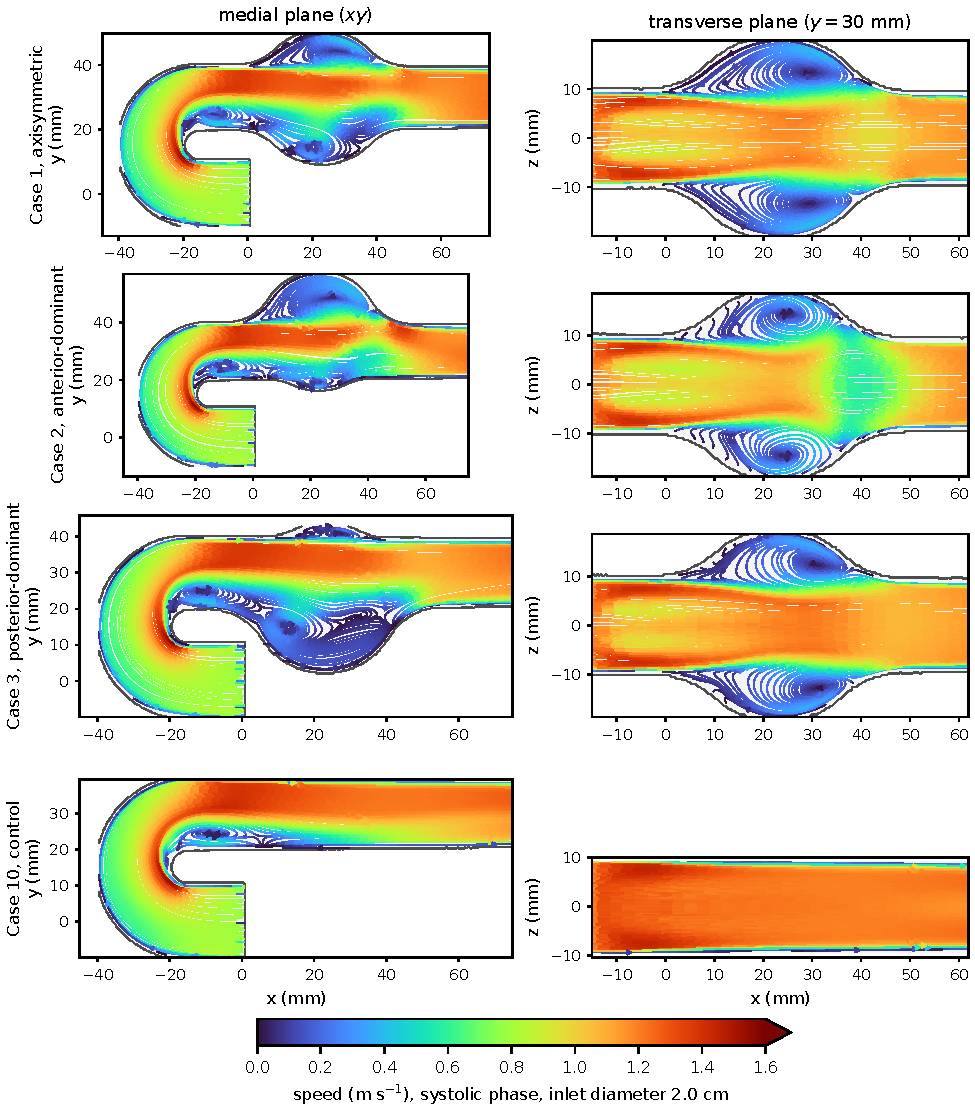
\includegraphics[width=0.92\textwidth]{streamlines_2p0.pdf}
\caption{Streamlines in the systolic phase for the 2.0~cm geometries in the medial plane (left) and the transverse plane (right), colored by in-plane speed on one scale for all geometries. Rows are the axisymmetric, anterior-dominant and posterior-dominant sacs and the control.}
\label{fig:streamlines_2p0}
\end{figure}

\begin{figure}[p]
\centering
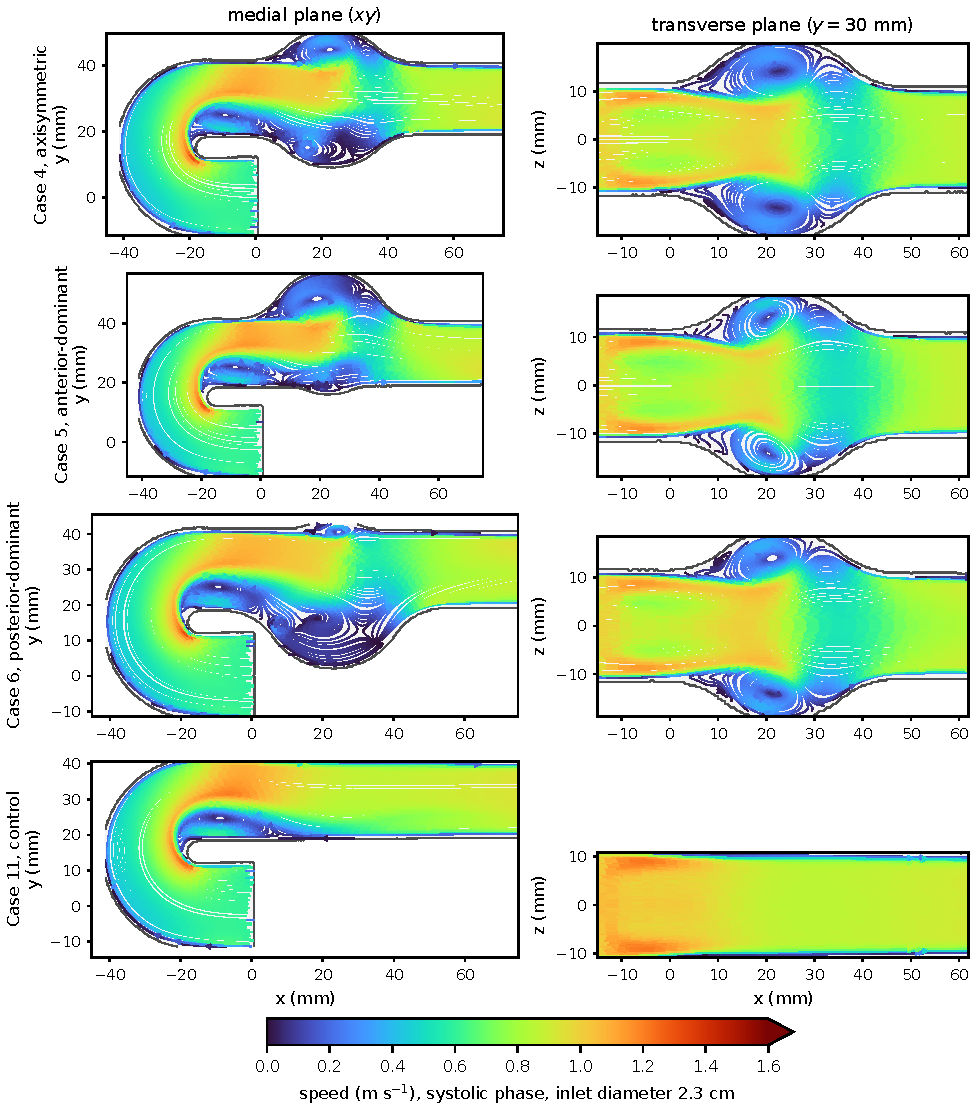
\includegraphics[width=0.92\textwidth]{streamlines_2p3.pdf}
\caption{As Figure~\ref{fig:streamlines_2p0}, for the 2.3~cm geometries.}
\label{fig:streamlines_2p3}
\end{figure}

\begin{figure}[p]
\centering
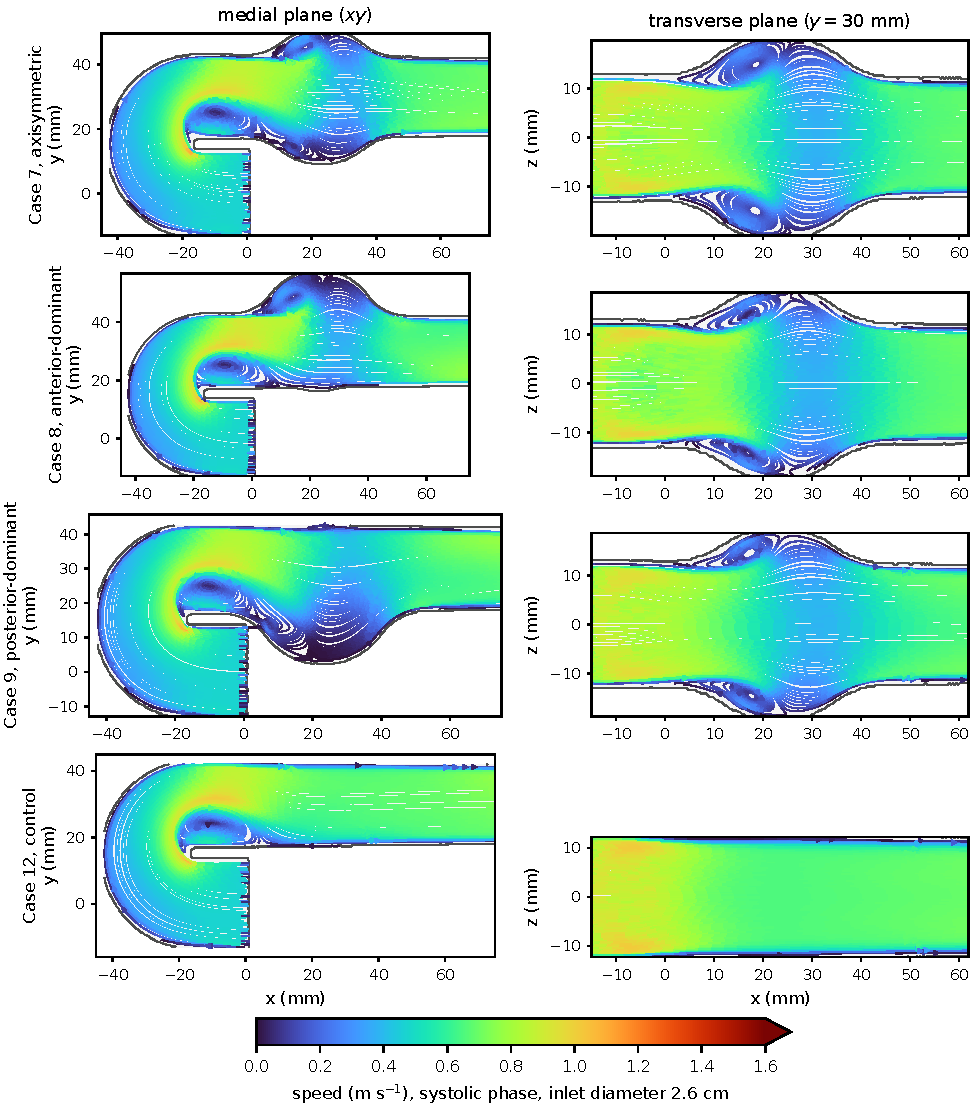
\includegraphics[width=0.92\textwidth]{streamlines_2p6.pdf}
\caption{As Figure~\ref{fig:streamlines_2p0}, for the 2.6~cm geometries.}
\label{fig:streamlines_2p6}
\end{figure}


\subsection{Pressure drop, reversed flow and eddy viscosity}
Table~\ref{tab:cfd_summary} summarizes the common-time flow descriptors for all twelve geometries, and inlet diameter clearly dominates the systolic response. The inlet-to-outlet pressure drop in the systolic phase decreases from \(1261\)--\(1346\,\mathrm{Pa}\) at \(2.0\,\mathrm{cm}\) to \(844\)--\(870\,\mathrm{Pa}\) at \(2.3\,\mathrm{cm}\) and \(528\)--\(561\,\mathrm{Pa}\) at \(2.6\,\mathrm{cm}\), whereas at a fixed diameter the three bulge patterns differ by at most \(7\%\). Relative to the matched control, the dilation adds \(17\)--\(30\%\) to the pressure drop. The fraction of dilation-segment nodes exhibiting reversed axial velocity at systole follows the same ordering, falling from \(50\)--\(54\%\) at \(2.0\,\mathrm{cm}\) to \(38\)--\(40\%\) at \(2.3\,\mathrm{cm}\) and \(24\)--\(28\%\) at \(2.6\,\mathrm{cm}\), against only \(2\)--\(3\%\) in the controls. The mean eddy viscosity within the segment is \(8.6\)--\(9.5\) times the molecular viscosity at \(2.0\,\mathrm{cm}\) but only \(1.6\)--\(2.1\) times at \(2.6\,\mathrm{cm}\). A narrower parent vessel therefore delivers a faster jet into the same \(4.0\,\mathrm{cm}\) sac, producing a larger expansion, a greater fraction of reversed flow, and stronger modeled turbulent mixing. At diastole, by contrast, the pressure drops are only \(1.6\)--\(10.7\,\mathrm{Pa}\), and \(35\)--\(47\%\) of the segment carries reversed flow in every geometry, including the controls, because the slow plateau flow no longer possesses a coherent core.

% Generated by generate_cfd_summary.py from data/processed/full (rigid-wall CFD); CSV: report/tables/eacfm_cfd_summary.csv
\begin{table}[htbp]
\centering
\small
\setlength{\tabcolsep}{3.2pt}
\caption{Common-time descriptors of the rigid-wall \CFD at systole (1.780~s) and
diastole (2.400~s). $\Delta p$ is the difference between the mean static pressure
on the inlet and outlet faces, and the reversed-flow fraction is the fraction of
nodes with $u_x<0$, the local downstream direction in the straight segment. The
evaluation segment is the dilation segment of Section~\ref{sec:exports}; all values
are node-weighted descriptive summaries of single designed geometries.}
\label{tab:cfd_summary}
\resizebox{\textwidth}{!}{%
\begin{tabular}{ccc rr cc cc c cc c}
\toprule
 & & & \multicolumn{2}{c}{$\Delta p$ (Pa)} & \multicolumn{2}{c}{Systolic $\tau_w$ (Pa)} & \multicolumn{2}{c}{Diastolic $\tau_w$ (Pa)} & Mean speed & \multicolumn{2}{c}{Reversed flow (\%)} & $\overline{\mu_t}/\mu$ \\
\cmidrule(lr){4-5}\cmidrule(lr){6-7}\cmidrule(lr){8-9}\cmidrule(lr){11-12}
Case & $D_{\rm in}$ (cm) & $\beta$ & Sys. & Dia. & Median & 95th pct. & Median & 95th pct. & sys. (m~s$^{-1}$) & Sys. & Dia. & sys. \\
\midrule
1 & 2.0 & 1.00 & 1261 & 10.7 & 1.94 & 17.6 & 0.279 & 0.60 & 0.362 & 50 & 35 & 9.5 \\
2 & 2.0 & 0.48 & 1346 & 3.1 & 2.83 & 17.4 & 0.729 & 1.07 & 0.391 & 50 & 45 & 9.4 \\
3 & 2.0 & 2.08 & 1297 & 5.7 & 1.65 & 15.4 & 0.851 & 1.24 & 0.346 & 54 & 45 & 8.6 \\
4 & 2.3 & 1.00 & 844 & 6.8 & 2.30 & 11.7 & 0.253 & 0.46 & 0.328 & 39 & 37 & 3.6 \\
5 & 2.3 & 0.48 & 870 & 1.7 & 2.39 & 10.7 & 0.613 & 0.98 & 0.330 & 38 & 46 & 4.0 \\
6 & 2.3 & 2.08 & 870 & 7.0 & 2.06 & 10.8 & 0.486 & 0.89 & 0.316 & 40 & 43 & 3.2 \\
7 & 2.6 & 1.00 & 545 & 4.9 & 1.87 & 8.1 & 0.251 & 0.59 & 0.275 & 28 & 38 & 1.6 \\
8 & 2.6 & 0.48 & 561 & 1.6 & 1.85 & 7.4 & 0.515 & 0.83 & 0.274 & 28 & 46 & 2.0 \\
9 & 2.6 & 2.08 & 528 & 5.8 & 1.82 & 7.1 & 0.447 & 0.91 & 0.261 & 24 & 47 & 2.1 \\
10 & 2.0 & Control & 1074 & 6.6 & 5.02 & 8.8 & 0.125 & 0.52 & 0.730 & 2 & 35 & 4.2 \\
11 & 2.3 & Control & 668 & 2.8 & 3.53 & 4.9 & 0.103 & 0.38 & 0.546 & 3 & 41 & 2.6 \\
12 & 2.6 & Control & 448 & 1.7 & 2.65 & 3.5 & 0.172 & 0.30 & 0.434 & 3 & 43 & 2.0 \\
\bottomrule
\end{tabular}%
}
\end{table}


\subsection{Wall shear stress}
Figure~\ref{fig:wss_sys} illustrates the \WSS magnitude over the dilation segment in the systolic phase, unwrapped about the axis of the descending segment. In this representation the anterior wall lies at \(0^\circ\) and the posterior wall at \(\pm180^\circ\), so that the full circumference of the vessel is displayed on a single plane. At systole all aneurysmal cases share a low-shear sac body bounded by high-shear rings at the proximal and distal necks, where the jet enters the sac and reattaches. The median segment \WSS is 1.6--2.8~Pa in the aneurysmal cases against 2.7--5.0~Pa in the controls, whereas the 95th percentile is 1.8--2.4 times that of the matched control (Table~\ref{tab:cfd_summary}). The neck rings weaken with increasing inlet diameter, and the 95th percentile falls from 15--18~Pa at 2.0~cm to 7--8~Pa at 2.6~cm. Asymmetry moves the pattern rather than scaling it. In the anterior-dominant cases the low-shear region is centered on the anterior wall (\(0^\circ\)), whereas in the posterior-dominant cases it is centered on the posterior wall (\(\pm180^\circ\)), so that over the sac body the wall opposite the dominant bulge carries the higher shear. In Case~2 the median sac-body \WSS is 4.5~Pa on the posterior wall against 0.9~Pa on the anterior bulge, and in Case~3 the 95th percentile is 8.4~Pa on the anterior wall against 2.1~Pa on the posterior bulge, with the same ordering in Cases~5, 6 and 9 and nearly equal values in Case~8. This behavior is consistent with the streamlines, which show that the jet crossing the sac impinges on the wall opposite the bulge while the bulge itself is filled by slow recirculating flow. At the distal neck the highest shear lies on the anterior (outer-curvature) side in most cases, irrespective of the bulge direction, because the core leaves the bend along the anterior wall.

Figure~\ref{fig:wss_dia} presents the same \WSS magnitude in the diastolic phase on one color scale per phase. At diastole the effect of asymmetry becomes larger than that of diameter. The median segment \WSS of the asymmetric sacs is 0.45--0.85~Pa, which is 1.8--3.1 times that of the axisymmetric sacs (0.25--0.28~Pa) at every diameter and 2.6--6.8 times that of the controls (0.10--0.17~Pa). On comparison of all cases, the diastolic maps show broad shear over the whole wall of the asymmetric sacs, consistent with a residual vortex that keeps moving along the sac wall during the plateau, whereas the axisymmetric sacs and the controls are close to stagnant. These are instantaneous values at two instants; the cycle-averaged picture is given by the \TAWSS maps in Section~\ref{sec:tawss}.

\begin{figure}[!htb]
\centering
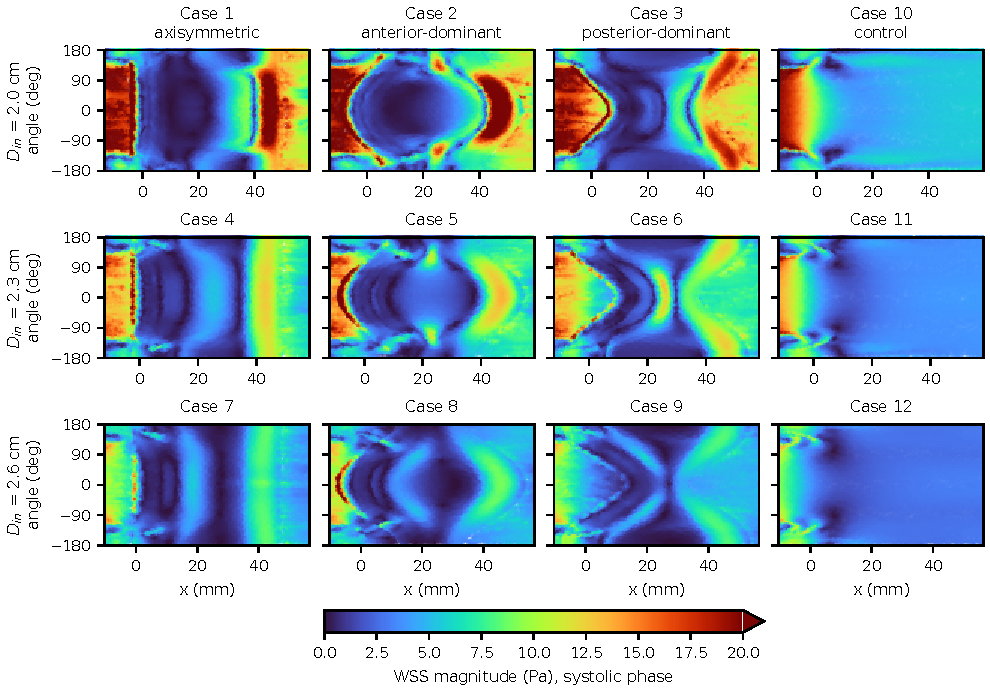
\includegraphics[width=\textwidth]{wss_montage_systole.pdf}
\caption{\WSS magnitude on the dilation segment in the systolic phase, on one color scale saturating at 20~Pa. The wall is unwrapped about the vessel axis, with the anterior wall at \(0^\circ\) and the posterior wall at \(\pm180^\circ\). Rows are inlet diameters and the last column is the matching control. White points are gaps in the exported wall nodes.}
\label{fig:wss_sys}
\end{figure}

\begin{figure}[!htb]
\centering
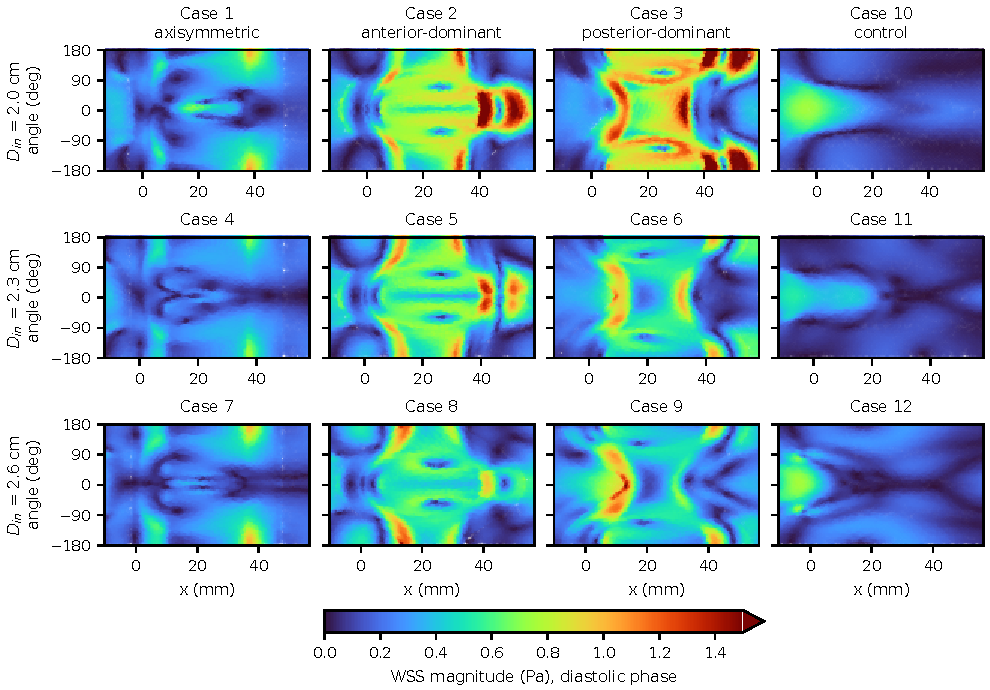
\includegraphics[width=\textwidth]{wss_montage_diastole.pdf}
\caption{As Figure~\ref{fig:wss_sys}, in the diastolic phase, with one color scale saturating at 1.5~Pa.}
\label{fig:wss_dia}
\end{figure}

Figure~\ref{fig:xwss} shows the signed axial component of \WSS for both the medial and transverse planes. Panel~(a) shows the \WSS on the anterior wall of the medial plane while panel~(b) shows the \WSS on the posterior wall of the medial plane. Panel~(c) shows the \WSS for the transverse plane. Because the aorta bends, a negative value alone does not prove local reverse flow in the curved segment, but along the straight descending segment the negative regions coincide with the recirculation seen in Figures~\ref{fig:streamlines_2p0}--\ref{fig:streamlines_2p6}. On the anterior medial wall and on the transverse wall, \WSS is large and positive at the proximal neck in every case. It becomes negative where the flow detaches on entering the sac, between \(x\approx-4\) and 16~mm on the anterior wall and between 0 and 4~mm on the transverse wall, and it stays negative over the recirculating part of the sac. It returns to positive values, marking reattachment of the core flow, between \(x\approx27\) and 42~mm on the anterior wall and between 26 and 39~mm on the transverse wall, followed by the high positive values of the distal neck. The reattachment point moves upstream as the inlet diameter increases, from 34--42~mm at 2.0~cm to 27--31~mm at 2.6~cm on the anterior wall and from 36--39~mm to 26--27~mm on the transverse wall, so the recirculation region shortens with a wider parent vessel, in line with the reversed-flow fractions of Table~\ref{tab:cfd_summary}. The posterior medial wall differs because \WSS is already negative at the proximal neck in every geometry, the controls included, which identifies this region as the \ICRZ rather than as part of the sac recirculation. The depth of the negative region does not follow the bulge pattern consistently; the most negative value inside the sac, \(-11.3\)~Pa, occurs on the anterior wall of Case~6.

\begin{figure}[!htb]
\centering
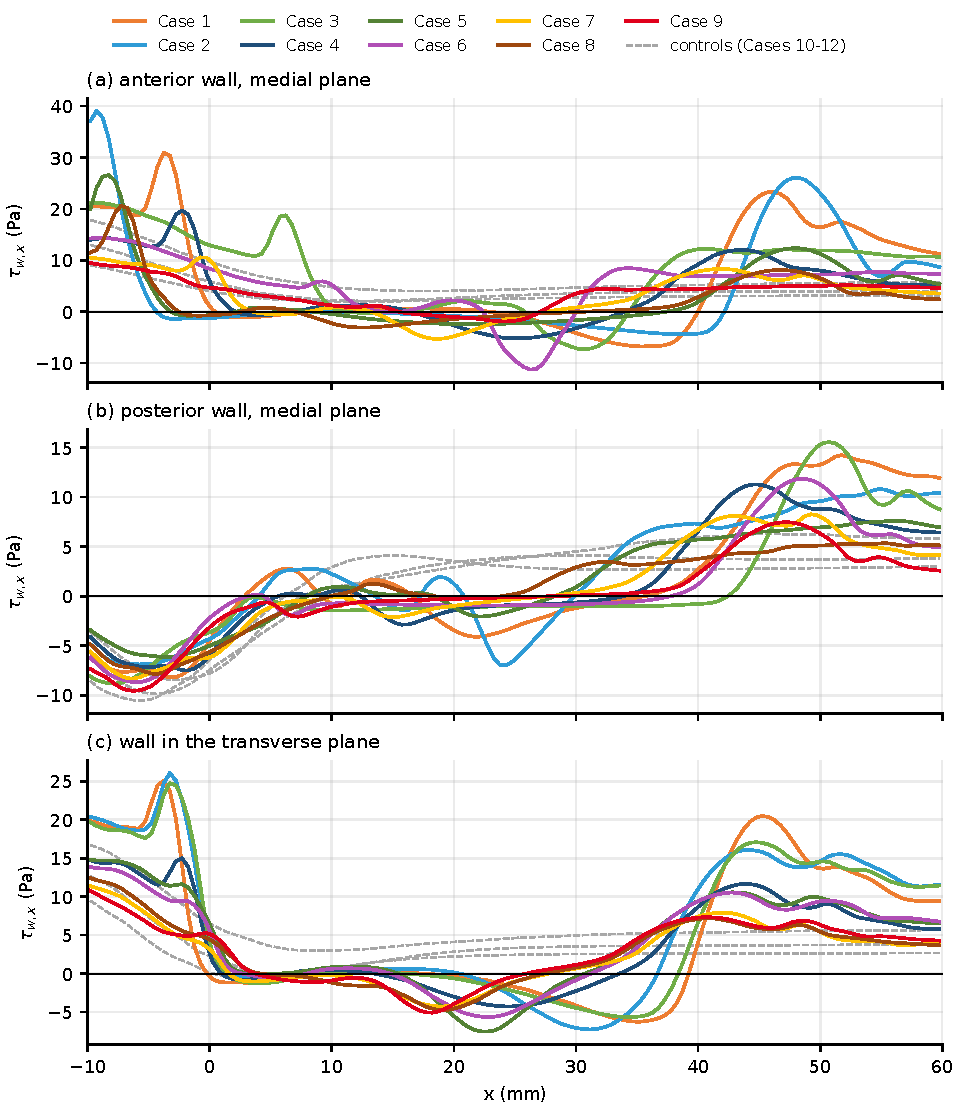
\includegraphics[width=0.85\textwidth]{xwss_lines.pdf}
\caption{Axial component of \WSS (Pa) along wall intersections with the medial and transverse planes at systole: (a) anterior medial wall, (b) posterior medial wall and (c) transverse-plane wall intersection.}
\label{fig:xwss}
\end{figure}

\subsection{Time-averaged wall shear stress}
\label{sec:tawss}

Figure~\ref{fig:tawss} and Table~\ref{tab:tawss} summarize \TAWSS across the twelve geometries. The \TAWSS is shown on the dilation segment of every geometry, unwrapped as in Figure~\ref{fig:wss_sys} and drawn on one logarithmic color scale because the values span two orders of magnitude. Every aneurysmal sac carries a broad region of low \TAWSS. The median over the dilation segment is 0.51--0.83~Pa in the aneurysmal cases against 2.5--4.5~Pa over the same stretch of the controls, while over the sac body the median on either side is 0.23--0.84~Pa. Relative to the matched control, the segment median is lower by a factor of 8.5--8.9 at 2.0~cm, 4.0--4.9 at 2.3~cm and 3.4--3.6 at 2.6~cm, so that the reduction in cycle-averaged shear caused by the dilation is largest for the narrowest parent vessel. The aneurysmal segment medians generally rise from the 2.0~cm group to the larger-diameter groups; the 95th percentiles and control medians decrease with inlet diameter. These statistics therefore describe different trends. The high-shear rings at the necks persist in the cycle average, and their strength falls with inlet diameter, the 95th percentile decreasing from 7.6--10.9~Pa at 2.0~cm to 5.5--6.4~Pa at 2.3~cm and 4.1--5.1~Pa at 2.6~cm.

Aneurysm asymmetry had a strong influence on the spatial distribution of \TAWSS. In asymmetric models, the lowest \TAWSS is usually located on the dominant bulge. In the anterior-dominant Cases~2, 5 and 8 the sac-body median is 0.34, 0.23 and 0.33~Pa on the anterior wall against 0.52, 0.58 and 0.84~Pa on the posterior wall, whereas in the posterior-dominant Cases~6 and 9 it is 0.24 and 0.28~Pa on the posterior wall against 0.71 and 0.60~Pa on the anterior wall. Case~3 is the exception, with similar values on both sides (0.35 and 0.42~Pa). In the axisymmetric sacs the low-shear region forms circumferential bands with nearly equal anterior and posterior medians. The bulge also has low instantaneous shear at systole. Together, these results show low systolic and low cycle-averaged shear; they do not establish that shear remains low at every instant or identify rupture-prone tissue. Low \TAWSS, in particular, marks regions of prolonged low shear, which are known to promote thrombus formation~\cite{salman2019biomechanical}, although the present models do not include those processes.

\begin{figure}[!htb]
\centering
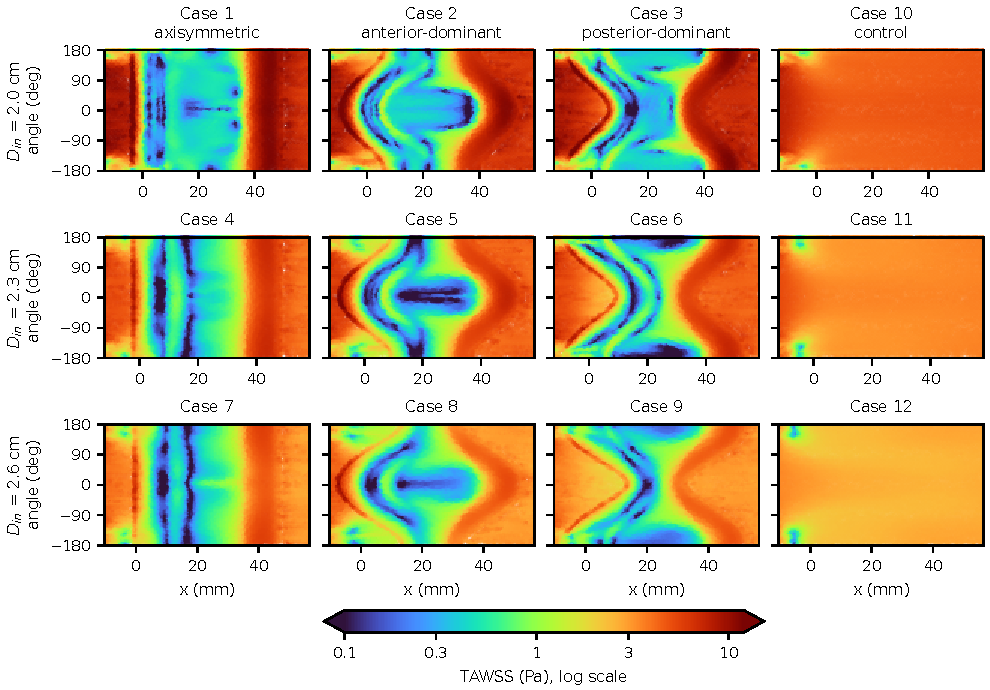
\includegraphics[width=\textwidth]{tawss_montage.pdf}
\caption{\TAWSScap on the dilation segment, unwrapped as in Figure~\ref{fig:wss_sys}, on one logarithmic color scale. Rows are inlet diameters and the last column is the matching control.}
\label{fig:tawss}
\end{figure}

% Generated by scripts/manuscript/generate_wss_montage.py from data/raw/TAWSS 30.09.2026.
\begin{table}[htbp]
\centering
\small
\caption{\revision{TAWSS (Pa) on the dilation segment. Percentiles are over the whole segment, while the sac-body medians use its middle third, within $60^\circ$ of the anterior or posterior direction.}}
\label{tab:tawss}
\begin{tabular}{cclccccc}
\toprule
 & & & \multicolumn{3}{c}{Segment} & \multicolumn{2}{c}{Sac body, median} \\
\cmidrule(lr){4-6}\cmidrule(lr){7-8}
Case & $D_{\rm in}$ (cm) & Morphology & 5th pct. & Median & 95th pct. & Anterior & Posterior \\
\midrule
1 & 2.0 & axisymmetric & 0.19 & 0.51 & 10.86 & 0.41 & 0.47 \\
2 & 2.0 & anterior-dominant & 0.15 & 0.52 & 7.60 & 0.34 & 0.52 \\
3 & 2.0 & posterior-dominant & 0.18 & 0.53 & 8.66 & 0.35 & 0.42 \\
10 & 2.0 & control & 3.65 & 4.53 & 4.89 & 4.66 & 4.36 \\
4 & 2.3 & axisymmetric & 0.12 & 0.70 & 6.41 & 0.47 & 0.49 \\
5 & 2.3 & anterior-dominant & 0.10 & 0.67 & 5.45 & 0.23 & 0.58 \\
6 & 2.3 & posterior-dominant & 0.10 & 0.83 & 5.82 & 0.71 & 0.24 \\
11 & 2.3 & control & 2.81 & 3.30 & 3.52 & 3.45 & 3.20 \\
7 & 2.6 & axisymmetric & 0.12 & 0.70 & 5.06 & 0.45 & 0.50 \\
8 & 2.6 & anterior-dominant & 0.17 & 0.73 & 4.12 & 0.33 & 0.84 \\
9 & 2.6 & posterior-dominant & 0.18 & 0.69 & 4.24 & 0.60 & 0.28 \\
12 & 2.6 & control & 2.20 & 2.51 & 2.82 & 2.59 & 2.51 \\
\bottomrule
\end{tabular}
\end{table}


\FloatBarrier

\subsection{Structural wall stress}
\label{sec:structural}

The structural calculation tests how pressure loading is distributed across the prescribed wall geometry. Diameter and asymmetry can alter tissue stress~\cite{vorp1998mechanical}, but stress alone does not determine failure because local wall strength is unknown. A Laplace-law estimate based on a uniform cylinder does not capture the changing curvature at an aneurysm's necks and crown; the three-dimensional structural model is used here to describe those stress concentrations.

Figure~\ref{fig:mps} presents the \MPS on the inner surface of the wall over the dilation segment, unwrapped as in Figure~\ref{fig:wss_sys}, and Table~\ref{tab:mps} summarizes it. In every aneurysmal case the \MPS is highest in circumferential bands at the necks, where the wall curvature changes sign, with 95th percentiles of 101--113~kPa over the necks, and lowest over the crown of the sac, where the medians are 55--80~kPa. This pattern is consistent with the findings of Vorp et al.~\cite{vorp1998mechanical}. The two morphology groups differ in their sac-body stress distribution. In the axisymmetric models, the stress was elevated at the proximal regions but lower at the midsection of the aneurysm sac, with similar behavior on both anterior and posterior sides; the anterior and posterior sac-body medians are within 1.2~kPa of each other. In contrast, the asymmetric models exhibited higher stress on the side opposite to the dominant bulge. The sac-body median on the posterior wall of the anterior-dominant Cases~2, 5 and 8 is 69.2, 73.6 and 78.1~kPa against 55.9, 55.0 and 61.8~kPa on the anterior bulge, and the anterior wall of the posterior-dominant Cases~3, 6 and 9 carries 68.3, 72.9 and 80.3~kPa against 55.8, 55.3 and 57.2~kPa on the posterior bulge. Median sac-body \MPS on the wall opposite the dominant bulge increases with inlet diameter. The controls show the same trend in segment-median \MPS (52.5, 58.4 and 65.1~kPa for inlet diameters of 2.0, 2.3 and 2.6~cm, respectively). This trend is consistent with greater tensile loading at a larger vessel radius under comparable pressure and wall thickness.

The controls have relatively uniform wall stress, with 95th percentiles within 3~kPa of their medians and mild elevations near the bend. In the asymmetric sacs, the wall opposite the dominant bulge has the higher sac-body median. Case~9 has the highest anterior sac-body median, 80.3~kPa; this is not a claim about the largest local peak. Indeed, the highest reported neck 95th percentile is 113.4~kPa in Case~5 (Table~\ref{tab:mps}). These are modeled loading patterns, obtained with a uniform 2~mm wall, literature material parameters and fixed ends. The retained records do not include the coupling-step settings, and local tissue strength is unknown, so the stress fields do not identify a failure site or quantify rupture risk.

\begin{figure}[!htb]
\centering
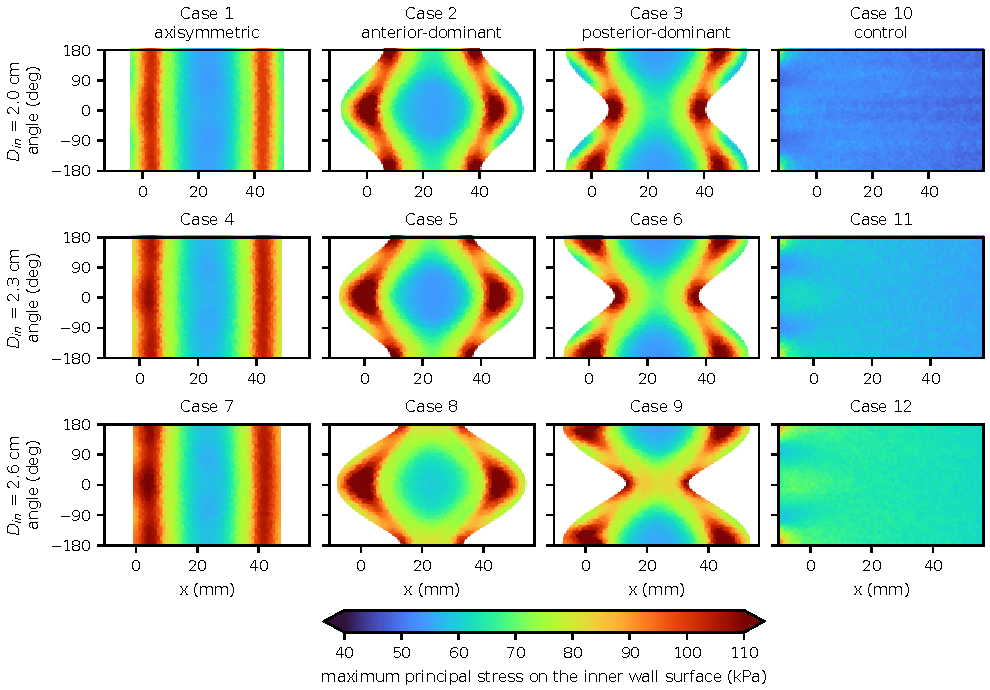
\includegraphics[width=\textwidth]{mps_montage.pdf}
\caption{\MPScap on the inner wall surface of the dilation segment, unwrapped as in Figure~\ref{fig:wss_sys}, on one color scale. Rows are inlet diameters and the last column is the matching control.}
\label{fig:mps}
\end{figure}

% Recomputed 2026-10-16 from data/raw/MPS; Case 8 uses the replacement data/Case 8.xls.
\begin{table}[htbp]
\centering
\small
\caption{\revision{Maximum principal stress (kPa) on the inner wall surface of the dilation segment. Sac-body medians use the middle third of the segment, within $60^\circ$ of the anterior or posterior direction, while the neck value is the 95th percentile over the outer thirds.}}
\label{tab:mps}
\begin{tabular}{cclccccc}
\toprule
 & & & \multicolumn{2}{c}{Segment} & \multicolumn{2}{c}{Sac body, median} & Necks \\
\cmidrule(lr){4-5}\cmidrule(lr){6-7}\cmidrule(lr){8-8}
Case & $D_{\rm in}$ (cm) & Morphology & Median & 95th pct. & Anterior & Posterior & 95th pct. \\
\midrule
1 & 2.0 & axisymmetric & 67.6 & 99.5 & 56.7 & 56.7 & 101.0 \\
2 & 2.0 & anterior-dominant & 70.2 & 106.9 & 55.9 & 69.2 & 111.3 \\
3 & 2.0 & posterior-dominant & 69.8 & 105.5 & 68.3 & 55.8 & 110.0 \\
10 & 2.0 & control & 52.5 & 54.8 & 52.4 & 52.8 & 54.9 \\
4 & 2.3 & axisymmetric & 71.4 & 103.9 & 58.1 & 59.0 & 104.5 \\
5 & 2.3 & anterior-dominant & 72.4 & 108.5 & 55.0 & 73.6 & 113.4 \\
6 & 2.3 & posterior-dominant & 72.2 & 107.4 & 72.9 & 55.3 & 112.1 \\
11 & 2.3 & control & 58.4 & 60.7 & 58.7 & 58.9 & 61.0 \\
7 & 2.6 & axisymmetric & 74.1 & 105.2 & 59.4 & 60.6 & 106.3 \\
8 & 2.6 & anterior-dominant & 75.9 & 111.6 & 55.3 & 80.5 & 117.7 \\
9 & 2.6 & posterior-dominant & 76.5 & 107.3 & 80.3 & 57.2 & 112.9 \\
12 & 2.6 & control & 65.1 & 67.6 & 65.3 & 65.7 & 68.0 \\
\bottomrule
\end{tabular}
\end{table}


\FloatBarrier

\subsection{Plane-wise flow summaries}
\label{sec:planes}

Plane-wise speed and \TKE summaries describe how the flow changes along the vessel and where the sac-associated disturbance persists downstream.

The eight planes are shown in Figure~\ref{fig:diagram}, and their diameters are listed in Table~\ref{tab:diameter}. Figure~\ref{fig:planes} shows the retained plane summaries for every case; Table~\ref{tab:plane_cfd} gives group medians. Speed is higher at D7--D8 than at D1--D3, consistent with the narrower distal lumen~\cite{kahveci2015numerical}. In the aneurysmal cases it falls to 0.10--0.16~m~s$^{-1}$ at D5, where every sac reaches 4.0~cm, compared with a control median of 0.193~m~s$^{-1}$, and recovers by D7. Continuity constrains cross-sectional mean axial velocity through flow rate and area; the plotted mean speed also reflects recirculation and the averaging used in the retained summaries. These prescribed-flow models do not test downstream perfusion.

Modeled $k$ rises through the sac, reaches about twice the control value at D5, remains elevated at D6--D7 and returns toward the control level at D8. The asymmetric sacs have higher D5 values than the axisymmetric sacs at each inlet diameter. These profiles are consistent with the sac recirculation and distal reattachment seen in the streamline maps~\cite{yu2000steady}. They locate the modeled disturbance but do not directly resolve the underlying turbulent fluctuations.

The plane summaries place the largest speed reduction at the sac center and the elevated modeled \TKE across the sac and its downstream region. They complement the wall quantities by describing the flow within the lumen. Because the slice workbook does not retain its averaging interval, these profiles are treated as descriptive summaries rather than independently verified cycle averages (Section~\ref{Limitations}).

\begin{figure}[!htb]
\centering
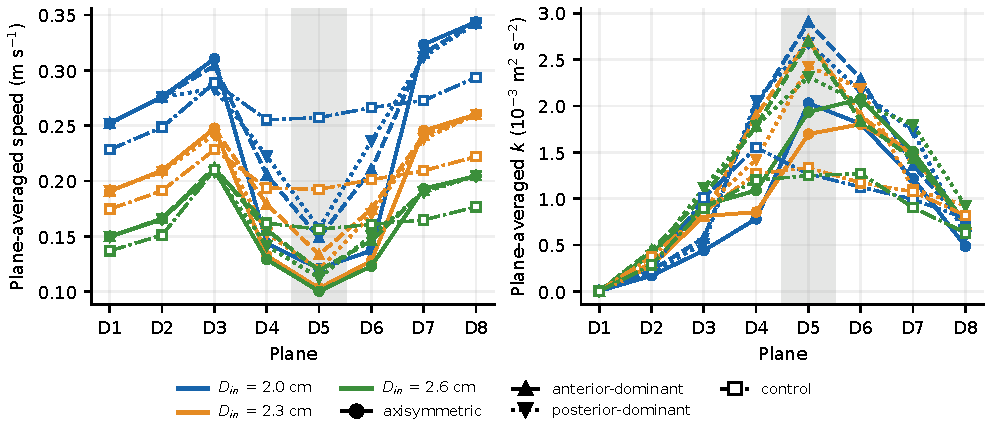
\includegraphics[width=\textwidth]{plane_profiles.pdf}
\caption{Plane-averaged speed (left) and \TKE per unit mass (right) at D1--D8 for all twelve geometries. Color gives the inlet diameter, and line style and marker the morphology; controls are dash-dot with open squares. The band marks the sac center (D5).}
\label{fig:planes}
\end{figure}

% Generated from corrected data/results_on_slices.csv on 2026-09-27.
\begin{table}[htbp]
\centering
\caption{Descriptive medians of the reported plane-averaged CFD quantities across nine aneurysmal and three control geometries. $k$ is turbulent kinetic energy per unit mass (m$^2$~s$^{-2}$). These designed cases do not support patient-population significance tests.}
\label{tab:plane_cfd}
\begin{tabular}{lcccc}
\toprule
& \multicolumn{2}{c}{Mean speed (m~s$^{-1}$)} & \multicolumn{2}{c}{$k$ ($10^{-3}$ m$^2$~s$^{-2}$)} \\
Plane & Aneurysmal & Control & Aneurysmal & Control \\
\midrule
D1 & 0.191 & 0.175 & 0.002 & 0.003 \\
D2 & 0.209 & 0.191 & 0.275 & 0.287 \\
D3 & 0.247 & 0.228 & 0.815 & 0.896 \\
D4 & 0.153 & 0.194 & 1.783 & 1.270 \\
D5 & 0.120 & 0.193 & 2.425 & 1.266 \\
D6 & 0.151 & 0.201 & 2.028 & 1.171 \\
D7 & 0.241 & 0.209 & 1.468 & 0.993 \\
D8 & 0.260 & 0.222 & 0.728 & 0.788 \\
\bottomrule
\end{tabular}
\end{table}


\section{Reconstruction results}
\label{sec:reconstruction_results}
\subsection{Checks on the complete \texorpdfstring{\CFD}{CFD} fields}
\label{sec:reference_results}
Before any fitting, the complete \CFD fields of the nine aneurysmal cases were used to check Eq.~\eqref{eq:momentum} and to measure the post-processing floors. With 40-neighbor least-squares gradients, the unsteady form with the \CFD eddy viscosity and without a $2\rho k/3$ term gave the smallest momentum residual in every case and phase, at 0.03--0.17 of the convective term in the bulk of the lumen. Omitting the time derivative raised the residual to 0.18--0.30 of convection at systole, and to 0.45--0.56 inside the sac, and to 0.49--0.73 at diastole, and adding the $2\rho k/3$ term made the residual larger. A quasi-steady momentum residual is therefore not consistent with these transient fields, particularly inside the sac.

Table~\ref{tab:reference_floor} gives the floors obtained by passing the complete \CFD velocity through the shared post-processing. Integrating the \CFD's own pressure gradient reproduces the \CFD pressure to 0.5--0.9\%, so the integration itself is accurate, and the remaining floor comes from the momentum terms. With the unsteady form and oracle $\mu_t$ the pressure floor is 1.6--2.3\% at systole, except for Case~2, whose forward window gives 7.1\%, and 2.2--4.1\% at diastole. Information matters differently in the two phases. At systole the molecular form is almost as good as the oracle for the 2.3 and 2.6~cm cases (1.8--2.7\%) but not for the 2.0~cm cases (4.9--11.3\%), in line with their larger eddy viscosity (Table~\ref{tab:cfd_summary}). At diastole removing either the time term or the eddy viscosity degrades the floor substantially, to 3.9--10.3\% and 9.0--19.3\%, respectively. The \WSS floor depends strongly on the distance $h$ in Eq.~\eqref{eq:wss_estimate}. At systole it is 0.07--0.09 at $h=0.1$~mm but 0.14--0.27 at the prespecified $h=0.25$~mm, because the systolic velocity profile is no longer close to quadratic over the $2h=0.5$~mm stencil, whereas at diastole it is 0.04--0.06 at either distance.

% Generated by generate_reference_table.py from the cfd run records.
\begin{table}[htbp]
\centering
\small
\setlength{\tabcolsep}{4pt}
\caption{\revision{\textcolor{red}{Pipeline floor, obtained by passing the complete CFD velocity through the shared post-processing. Pressure columns give the sub-cloud relative L2 error for each information setting, combining retention or omission of the time term with either CFD eddy viscosity or molecular viscosity alone. $\Delta p_{\rm sub}$ is the CFD pressure drop between the inlet and outlet ends of the sub-cloud. Wall-shear columns give the aneurysm-zone magnitude error of the one-sided estimate at $h=0.1$~mm and at the prespecified $h=0.25$~mm. Case 2's systolic window runs forward from the target (1.780--1.788~s), which explains its larger unsteady error.}}}
\label{tab:reference_floor}
\begin{tabular}{llccccrcc}
\toprule
 & & \multicolumn{4}{c}{Pressure relative L2} & & \multicolumn{2}{c}{Wall shear} \\
\cmidrule(lr){3-6}\cmidrule(lr){8-9}
Case & Phase & Unst.+$\mu_t$ & Steady+$\mu_t$ & Unst.+$\mu$ & Steady+$\mu$ & $\Delta p_{\rm sub}$ (Pa) & $h=0.1$ & $h=0.25$ \\
\midrule
1 & Sys. & 0.022 & 0.031 & 0.049 & 0.067 & 986.1 & 0.086 & 0.249 \\
1 & Dia. & 0.035 & 0.074 & 0.152 & 0.188 & 8.8 & 0.044 & 0.042 \\
2 & Sys. & 0.071 & 0.027 & 0.113 & 0.048 & 1063.4 & 0.090 & 0.273 \\
2 & Dia. & 0.037 & 0.056 & 0.145 & 0.154 & 1.1 & 0.048 & 0.042 \\
3 & Sys. & 0.022 & 0.029 & 0.065 & 0.071 & 1010.2 & 0.090 & 0.220 \\
3 & Dia. & 0.024 & 0.039 & 0.091 & 0.101 & 3.7 & 0.048 & 0.046 \\
4 & Sys. & 0.019 & 0.037 & 0.023 & 0.036 & 664.2 & 0.077 & 0.182 \\
4 & Dia. & 0.032 & 0.103 & 0.175 & 0.242 & 5.5 & 0.050 & 0.037 \\
5 & Sys. & 0.019 & 0.036 & 0.027 & 0.036 & 682.4 & 0.094 & 0.208 \\
5 & Dia. & 0.031 & 0.051 & 0.114 & 0.121 & 0.4 & 0.052 & 0.041 \\
6 & Sys. & 0.018 & 0.033 & 0.026 & 0.032 & 685.4 & 0.078 & 0.191 \\
6 & Dia. & 0.041 & 0.068 & 0.193 & 0.211 & 5.8 & 0.054 & 0.042 \\
7 & Sys. & 0.016 & 0.037 & 0.018 & 0.035 & 412.8 & 0.070 & 0.151 \\
7 & Dia. & 0.038 & 0.090 & 0.172 & 0.246 & 4.1 & 0.050 & 0.040 \\
8 & Sys. & 0.023 & 0.048 & 0.018 & 0.042 & 422.4 & 0.090 & 0.183 \\
8 & Dia. & 0.039 & 0.065 & 0.154 & 0.160 & 0.6 & 0.055 & 0.043 \\
9 & Sys. & 0.020 & 0.033 & 0.020 & 0.033 & 397.3 & 0.070 & 0.141 \\
9 & Dia. & 0.022 & 0.045 & 0.090 & 0.096 & 4.8 & 0.060 & 0.048 \\
\bottomrule
\end{tabular}
\end{table}


\subsection{Momentum-constrained \texorpdfstring{\PINNs}{PINNs} on the development geometries}
\label{sec:pilot_results}
In the development cases, every neural field reconstructed the hidden velocity three to four times more accurately than \RBF (relative errors 0.037--0.052 versus 0.13--0.16 at systole) and five times more accurately than linear interpolation. However, the prespecified criterion of the development test failed on both endpoints (Table~\ref{tab:pilot}). The momentum arms were trained with a blood density of 1060~kg~m$^{-3}$ in the scaling of their residual before the density was corrected to 1050~kg~m$^{-3}$; all reported scores use the corrected value, The difference is about 1\%, but its effect on optimization was not tested by retraining. The gate scored the momentum \PINNs by their own pressure output and automatic-differentiation \WSS, the direct route that a \PINN offers, and the other methods by shared post-processing, so the comparison changes both the fitting and the pressure route. The unsteady \PINN's own pressure output had errors of 0.43--0.53 at systole and 0.56--1.05 at diastole, and the steady \PINN's 0.51--0.90, whereas the continuity field passed through the shared integration reached 0.023--0.049. The \PINN's automatic-differentiation \WSS (0.40--0.45 at systole) was also worse than the pipeline \WSS of the continuity field (0.35--0.37).

Because the gate changed both the fitting and the pressure route, we also passed the velocity of every momentum \PINN through the shared post-processing (Table~\ref{tab:pilot_pipeline}). In the prespecified unsteady form the unsteady \PINN's velocity still gave pressure errors of 0.37--0.48 at systole and 0.58--1.11 at diastole, against 0.023--0.049 for the continuity field, because that form uses the difference between the field's two snapshots. Dropping the time term reduced the error to 0.037--0.089, still above the continuity field. The \PINN's momentum residual was an order of magnitude smaller than that of the continuity field (0.2 against 2.5 in scaled units), so the network satisfied the momentum balance by adjusting a time derivative that was constrained only at the observed nodes of two snapshots 5--10~ms apart. With so little temporal information, $\partial_t\mathbf u$ and the pressure act as slack variables in a soft momentum penalty rather than as information. The steady \PINN, whose loss does not contain a time derivative, came close to the continuity field only in the systolic window of Case~1 (0.029 against 0.025). For \WSS the shared estimate gave similar errors for all fields at systole (0.34--0.40), and the momentum \PINNs gave lower errors in the diastolic Case~9 window (0.11--0.12 against 0.22). Adding the momentum balance to the loss therefore did not improve the velocity used for pressure, although it helped \WSS in one diastolic window. The confirmation study therefore evaluated the continuity field with physics applied after fitting, as specified in Section~\ref{sec:protocol}.


\begin{table}[htbp]
\centering
\small
\caption{Pilot endpoints. The continuity field is scored through the shared post-processing, and the momentum PINNs through their own pressure output and automatic-differentiation WSS. Values average two draws at systole and one at diastole.}
\label{tab:pilot}
\begin{tabular}{llccccc}
\toprule
Case & Phase & \shortstack{Cont. pressure\\(post-proc.)} & \shortstack{Steady head\\(direct)} & \shortstack{Unsteady head\\(direct)} & \shortstack{Cont. shear\\(post-proc.)} & \shortstack{Unsteady shear\\(autograd)} \\
\midrule
1 & Sys. & 0.025 & 0.787 & 0.435 & 0.369 & 0.447 \\
1 & Dia. & 0.045 & 0.897 & 1.048 & 0.113 & 0.130 \\
9 & Sys. & 0.023 & 0.633 & 0.531 & 0.346 & 0.396 \\
9 & Dia. & 0.049 & 0.515 & 0.558 & 0.224 & 0.155 \\
\bottomrule
\end{tabular}
\end{table}

% Generated by scripts/manuscript/generate_pilot_pipeline.py.
\begin{table}[htbp]
\centering
\small
\caption{Pilot fields scored through the same post-processing. Pressure is the relative L2 error of momentum integration applied to each field's velocity, in the prespecified unsteady form with CFD eddy viscosity, and, for the unsteady PINN, also in the steady form, which does not use the field's time derivative. WSS is the finite-distance estimate at $h=0.25$~mm. All fields use the CFD eddy viscosity. Values are averaged over two draws at systole and one at diastole.}
\label{tab:pilot_pipeline}
\setlength{\tabcolsep}{4pt}
\begin{tabular}{llccccccc}
\toprule
 & & \multicolumn{4}{c}{Pressure} & \multicolumn{3}{c}{Aneurysm-zone WSS} \\
\cmidrule(lr){3-6}\cmidrule(lr){7-9}
Case & Phase & \shortstack{Cont.\\field} & \shortstack{Steady\\PINN} & \shortstack{Unsteady\\PINN} & \shortstack{Unsteady PINN,\\steady form} & \shortstack{Cont.\\field} & \shortstack{Steady\\PINN} & \shortstack{Unsteady\\PINN} \\
\midrule
1 & Sys. & 0.025 & 0.029 & 0.373 & 0.046 & 0.369 & 0.399 & 0.401 \\
1 & Dia. & 0.045 & 0.060 & 1.103 & 0.089 & 0.113 & 0.118 & 0.100 \\
9 & Sys. & 0.023 & 0.036 & 0.479 & 0.037 & 0.346 & 0.347 & 0.335 \\
9 & Dia. & 0.049 & 0.126 & 0.577 & 0.050 & 0.224 & 0.123 & 0.111 \\
\bottomrule
\end{tabular}
\end{table}


\subsection{Confirmation on seven held-out geometries}
\label{sec:confirmation}
At the primary 2.5~mm spacing the continuity field followed by the shared post-processing had lower pressure error than \RBF with the same post-processing in all 14 case--phase units, with a median ratio of 0.458, and lower aneurysm-zone \WSS error in all 14 units, with a median ratio of 0.508 (Table~\ref{tab:recon_summary}, Figure~\ref{fig:confirmation}). Both prespecified hypotheses were met, and the velocity guardrail held in every unit, with hidden-velocity errors of 0.033--0.050 against 0.113--0.169 for \RBF. At the level of individual draws the \WSS advantage held in 42 of 42 comparisons, whereas the pressure advantage held in 39 of 42. The prespecified decision rule was the count of units, and no significance test was planned. The draw-level counts are descriptive because draws and phases share geometries; they are not treated as independent replicates for significance testing. The three adverse pressure draws were all diastolic, in Case~4 (ratio 1.05), Case~7 (1.40) and Case~8 (1.75), and the case-wise tables in Appendix~\ref{app:casewise} show that the diastolic pressure error of the neural field varies between draws by up to 0.085, several times more than \RBF's.

\begin{table}[htbp]
\centering
\small
\caption{Median of seven case means at 2.5~mm; each reconstructed case mean uses three paired draws. Entries are node-weighted relative L2 errors. Pressure is conditional on oracle CFD eddy viscosity. Full CFD denotes the same post-processing applied to complete velocity; its error is a reference, not a strict lower bound.}
\label{tab:recon_summary}
\begin{tabular}{llccccc}
\toprule
Phase & Quantity & Continuity & Data-only & RBF & Linear & Full CFD \\
\midrule
Systole & Velocity & 0.044 & 0.052 & 0.146 & 0.226 & 0.000 \\
Systole & Pressure & 0.023 & 0.028 & 0.079 & 0.292 & 0.019 \\
Systole & Wall shear & 0.356 & 0.333 & 0.609 & 0.834 & 0.191 \\
Diastole & Velocity & 0.038 & 0.039 & 0.130 & 0.242 & 0.000 \\
Diastole & Pressure & 0.094 & 0.063 & 0.132 & 0.167 & 0.037 \\
Diastole & Wall shear & 0.163 & 0.161 & 0.374 & 0.615 & 0.042 \\
\bottomrule
\end{tabular}
\end{table}


\begin{figure}[!htb]
\centering
\begin{minipage}{0.48\textwidth}
\centering
\begin{tikzpicture}
\begin{axis}[width=0.90\linewidth,height=5.8cm,xmin=0,xmax=0.20,ymin=0,ymax=0.20,
 xlabel={\RBF pressure error},ylabel={Continuity-field pressure error},
 tick label style={font=\scriptsize},label style={font=\small},grid=major,
 legend style={font=\scriptsize,at={(0.03,0.97)},anchor=north west,draw=none}]
\addplot[black,dashed,forget plot] coordinates {(0,0) (0.20,0.20)};
\addplot[only marks,mark=*,blue] table[x=rbf,y=field]{figures/generated/confirm_p_sys.dat};
\addlegendentry{Systole}
\addplot[only marks,mark=square*,red] table[x=rbf,y=field]{figures/generated/confirm_p_dia.dat};
\addlegendentry{Diastole}
\end{axis}
\end{tikzpicture}
\end{minipage}
\hfill
\begin{minipage}{0.48\textwidth}
\centering
\begin{tikzpicture}
\begin{axis}[width=0.90\linewidth,height=5.8cm,xmin=0,xmax=0.75,ymin=0,ymax=0.75,
 xlabel={\RBF \WSS error},ylabel={Continuity-field \WSS error},
 tick label style={font=\scriptsize},label style={font=\small},grid=major]
\addplot[black,dashed,forget plot] coordinates {(0,0) (0.75,0.75)};
\addplot[only marks,mark=*,blue] table[x=rbf,y=field]{figures/generated/confirm_wss_sys.dat};
\addplot[only marks,mark=square*,red] table[x=rbf,y=field]{figures/generated/confirm_wss_dia.dat};
\end{axis}
\end{tikzpicture}
\end{minipage}
\caption{Case-wise confirmation errors for pressure (left, unsteady form with oracle $\mu_t$) and aneurysm-zone \WSS magnitude (right, $h=0.25$~mm) at 2.5~mm. Each point is one case--phase unit averaged over three paired draws; points below the diagonal favor the continuity field. Both pipelines receive the same oracle eddy viscosity.}
\label{fig:confirmation}
\end{figure}

The phases differ in how close the reconstruction comes to its floor. At systole the median pressure error of the continuity field, 0.023, is close to the floor of 0.019, so the reconstructed velocity is good enough that the post-processing, not the reconstruction, sets most of the pressure error. At diastole the median error of 0.094 is two and a half times the floor of 0.037, and the advantage over \RBF (0.132) is small in Cases~7 and 8 (0.155 against 0.171 and 0.101 against 0.104). The median systolic \WSS error of 0.356 lies well above its floor of 0.191, and the diastolic 0.163 lies well above 0.042, so for \WSS the reconstruction remains the limiting step.

\subsection{Local errors and field maps}
\label{sec:local}
Global relative errors can hide local failures, so Table~\ref{tab:local_metrics} and Figures~\ref{fig:velocity_maps}--\ref{fig:field_maps_adverse} report local measures. The 95th percentile of the pointwise velocity error magnitude in systole is 0.057~m~s$^{-1}$ for the continuity field and 0.20~m~s$^{-1}$ for \RBF, against peak speeds of about 1.0--1.6~m~s$^{-1}$, and within the sac the relative velocity error is 0.075 against 0.185. The largest pointwise velocity errors of the continuity field lie in the thin shear layer where the flow separates at the bend exit (Figure~\ref{fig:velocity_maps}).

\begin{table}[htbp]
\centering
\small
\caption{\revision{Additional error measures at 2.5~mm, reported as medians of seven case means, with velocity p95 denoting the 95th percentile of pointwise vector-error magnitude and sac velocity reported as relative L2. The shear ratio compares predicted and CFD 99th percentiles, while pressure-drop error is averaged in absolute value within each case before taking the median.}}
\label{tab:local_metrics}
\begin{tabular}{llcccc}
\toprule
Phase & Method & Velocity p95 & Sac velocity & Shear q99 ratio & Drop error \\ & & (m/s) & rel. L2 & & (Pa) \\
\midrule
Systole & Continuity & 0.0569 & 0.075 & 0.923 & 5.57 \\
Systole & Data-only & 0.0657 & 0.082 & 0.956 & 8.64 \\
Systole & RBF & 0.2005 & 0.185 & 0.520 & 30.59 \\
Diastole & Continuity & 0.0056 & 0.040 & 0.897 & 0.48 \\
Diastole & Data-only & 0.0057 & 0.041 & 1.001 & 0.47 \\
Diastole & RBF & 0.0206 & 0.143 & 0.611 & 0.67 \\
\bottomrule
\end{tabular}
\end{table}


\begin{figure}[H]
\centering
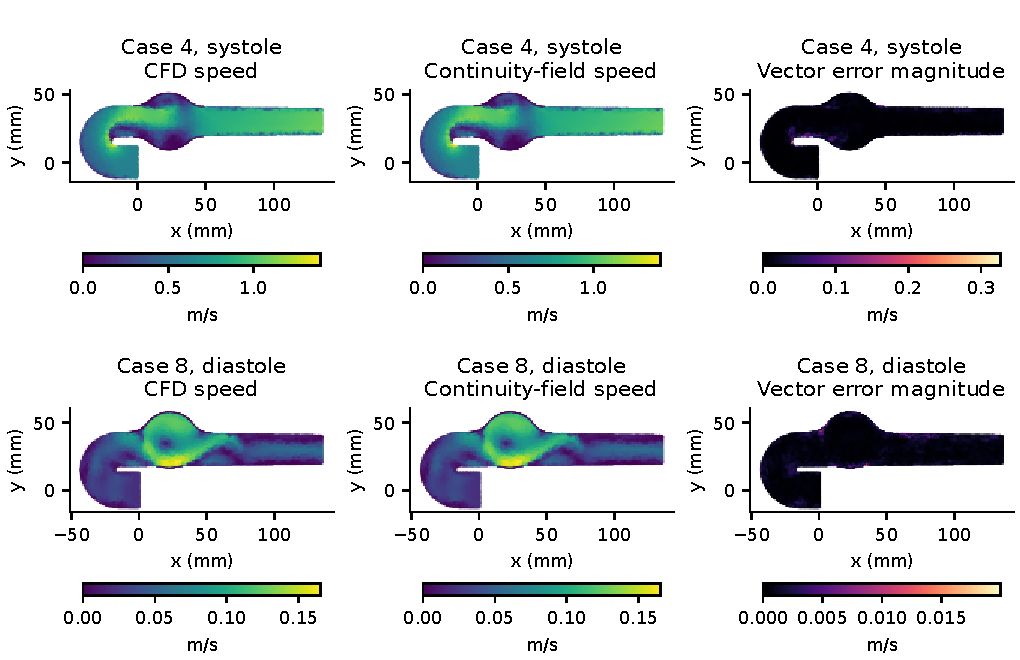
\includegraphics[width=0.90\textwidth]{hidden_velocity_examples.pdf}
\caption{Hidden-node speed on the mid-plane ($|z-z_{\rm mid}|<0.35$~mm) for Case~4 at systole and Case~8 at diastole (draw 0, 2.5~mm). Left, \CFD; center, continuity field; right, magnitude of the vector error. Only unobserved nodes are shown.}
\label{fig:velocity_maps}
\end{figure}

The 99th percentile of aneurysm-zone \WSS is recovered to 0.92 of the \CFD value at systole and 0.90 at diastole, whereas \RBF recovers only 0.52 and 0.61 of it, so \RBF's \WSS error consists mostly of flattened peaks. The Pearson correlation between reconstructed and \CFD \WSS magnitude is 0.92 at systole and 0.94 at diastole for the continuity field, against 0.87 and 0.79 for \RBF, and the \WSS vector errors are 0.38 and 0.20 against 0.62 and 0.42. The systolic pressure drop, which ranges from 413 to 1063~Pa across the cases, is recovered with a median absolute error of 6~Pa against 31~Pa for \RBF. At diastole the median drop errors of 0.48 and 0.67~Pa are comparable to the drops themselves (0.4--5.8~Pa), so neither method recovers the diastolic drop reliably, even though the relative error over the whole pressure field is modest.

The two kinds of error also differ in form. In the median systolic unit (Figure~\ref{fig:field_maps}) the continuity field reproduces the \WSS rings at both necks, while \RBF smears them and underestimates their peaks.

\begin{figure}[H]
\centering
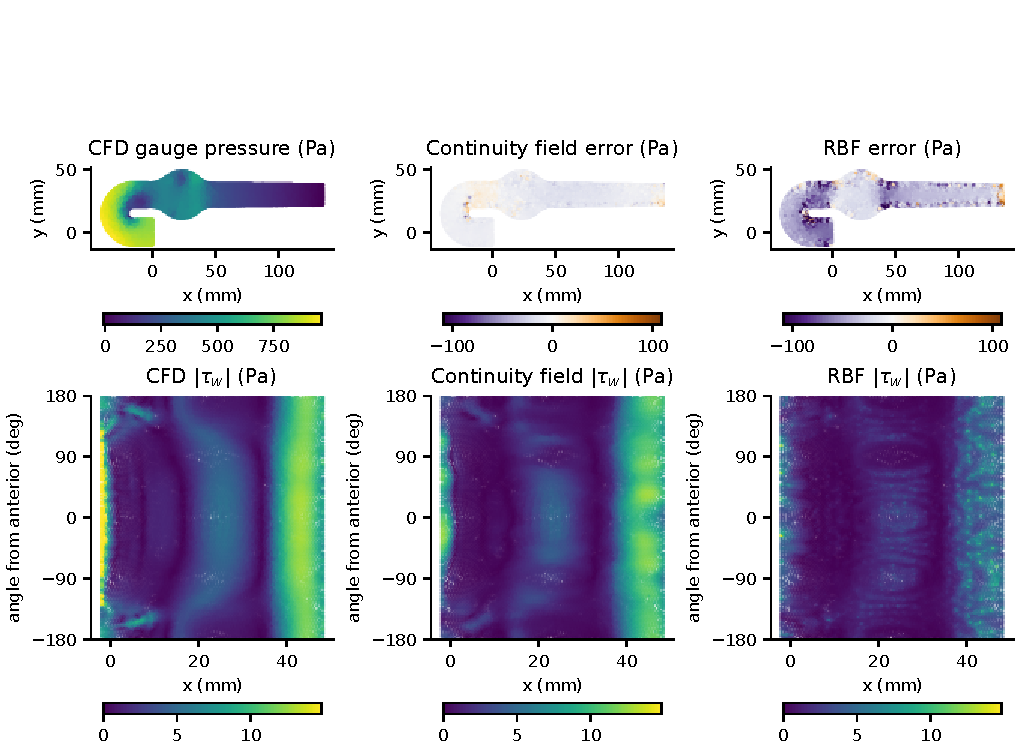
\includegraphics[width=0.95\textwidth]{field_maps_c04_t1780.pdf}
\caption{Case~4 at systole (draw 0, 2.5~mm), close to the median result. Top, \CFD mid-plane pressure and the pressure errors of the continuity field and \RBF. Bottom, aneurysm-zone \WSS unwrapped about the vessel axis. Relative errors are 0.024 and 0.100 for pressure and 0.32 and 0.60 for \WSS.}
\label{fig:field_maps}
\end{figure}

In the adverse diastolic unit (Figure~\ref{fig:field_maps_adverse}), the continuity field's pressure error is a smooth offset of about 1~Pa that accumulates along the vessel, which points to a small bias in the integrated pressure gradient such as the two-snapshot acceleration, while \RBF's pressure errors are concentrated near the sac necks.

\begin{figure}[H]
\centering
\IfFileExists{figures/generated/field_maps_c07_t2400.pdf}{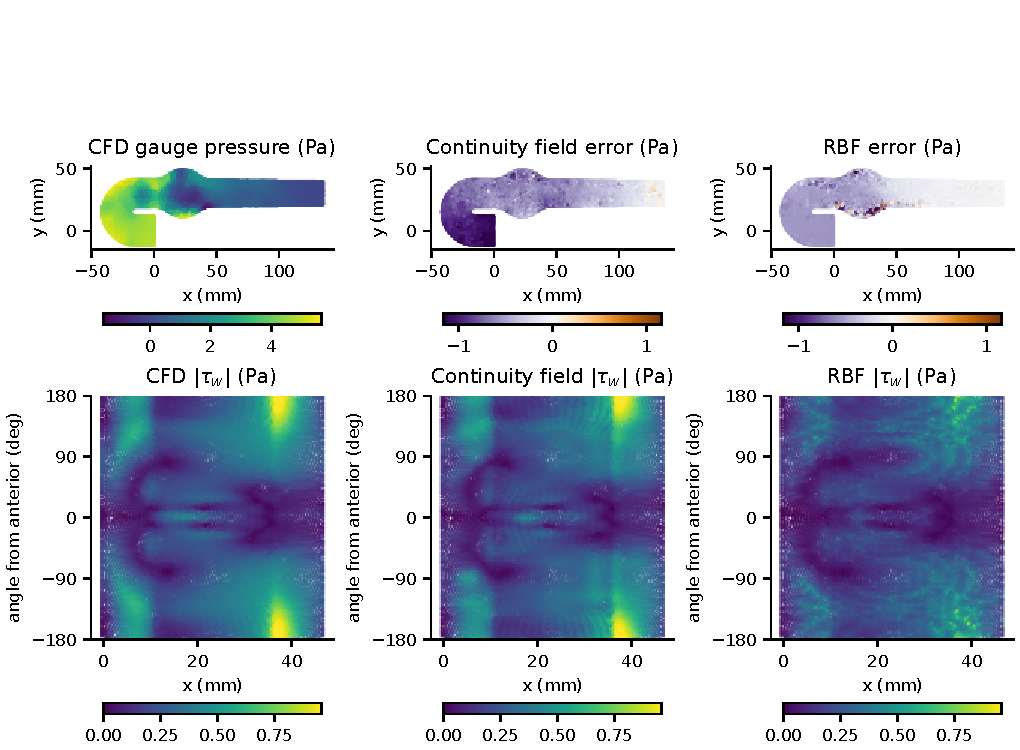
\includegraphics[width=0.95\textwidth]{field_maps_c07_t2400.pdf}}{\fbox{Case 7 diastolic maps pending}}
\caption{As Figure~\ref{fig:field_maps}, for the adverse unit Case~7 at diastole. Relative errors are 0.25 and 0.18 for pressure and 0.14 and 0.33 for \WSS. The \CFD pressure varies by only a few pascals, so errors of about 1~Pa dominate.}
\label{fig:field_maps_adverse}
\end{figure}

The \WSS calculated by automatic differentiation of the continuity field itself was worse than the finite-distance estimate from the same field (median 0.55 against 0.36 in systole and 0.27 against 0.16 in diastole). The soft no-slip penalty fixes the velocity at the wall but leaves its wall-normal gradient poorly determined, so the network's analytic derivative should not be read as \WSS. The finite-distance estimate is also sensitive to $h$. Evaluated at 0.1~mm instead of 0.25~mm, the continuity field's median systolic \WSS error falls from 0.356 to 0.326, and at 0.5~mm it rises to 0.476. We keep the prespecified distance because choosing $h$ with knowledge of the \WSS target would be information that a deployment does not have.

\subsection{Contribution of the continuity penalty and sampling density}
\label{sec:ablation}
Figure~\ref{fig:budget} separates the effect of the continuity penalty from that of the neural representation. At 2.5~mm, the data field without an interior PDE penalty is close to the continuity field, with median velocity errors of 0.052 and 0.039 versus 0.044 and 0.038, and is slightly better on two endpoints, diastolic pressure (0.063 versus 0.094) and systolic \WSS (0.333 versus 0.356). At the densest spacing of 1.5~mm the data field is better on every endpoint except systolic pressure. Only at the sparsest spacing of 4.0~mm, where the observations cover 0.34--0.37\% of the nodes, does the continuity penalty help consistently, reducing the median hidden-velocity error from 0.125 to 0.077 at systole and from 0.105 to 0.077 at diastole, the systolic pressure error from 0.072 to 0.052 and the diastolic \WSS error from 0.371 to 0.316. The main advantage over \RBF therefore comes from fitting one smooth space-time representation to both snapshots, and continuity becomes useful when the data alone no longer determine the field.

The advantage of both neural fields over \RBF grows as the observations become sparser. The median systolic pressure errors at 1.5, 2.5 and 4.0~mm are 0.024, 0.023 and 0.052 for the continuity field versus 0.029, 0.079 and 0.178 for \RBF, and the median systolic \WSS errors are 0.30, 0.36 and 0.48 versus 0.49, 0.61 and 0.68. At diastole and 4.0~mm the continuity field's pressure error is 0.096 versus 0.318 for \RBF. Only one draw was performed at 1.5 and 4.0~mm, so these values describe a trend rather than an uncertainty interval.

\begin{figure}[H]
\centering
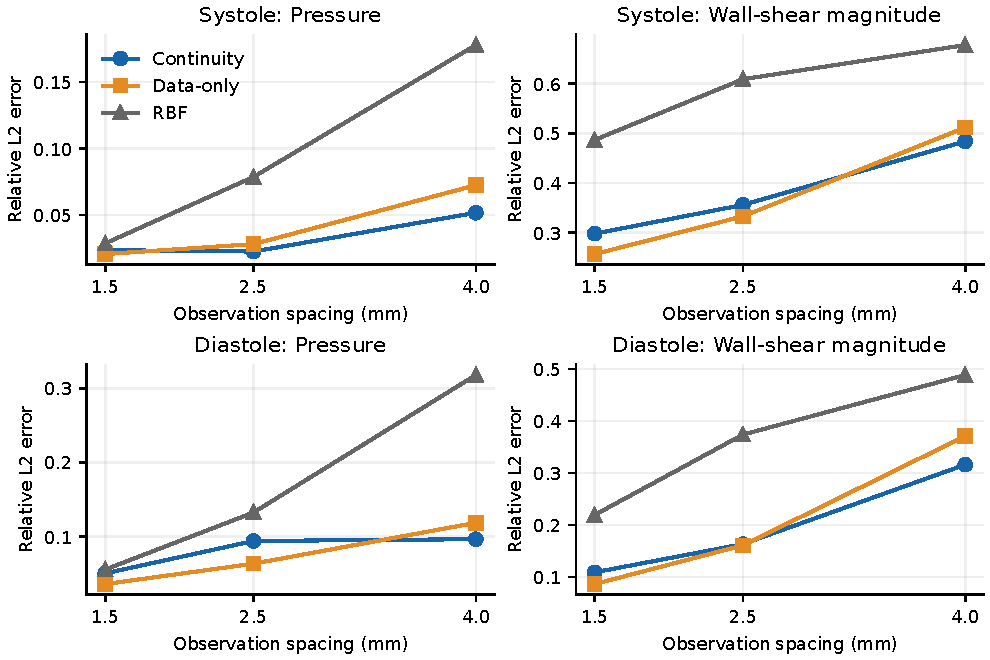
\includegraphics[width=0.92\textwidth]{observation_budget.pdf}
\caption{Median pressure (unsteady form with oracle $\mu_t$) and aneurysm-zone \WSS errors over Cases~2--8 against observation spacing. The 2.5~mm values average three draws per case; 1.5 and 4.0~mm use one draw.}
\label{fig:budget}
\end{figure}

Figure~\ref{fig:pressure_information} asks two separate questions about pressure recovery, namely whether to retain the local acceleration term and whether to supply the \CFD eddy viscosity. Here, steady and unsteady refer to the pressure calculation applied after reconstruction, not to separately trained neural fields. In the seven confirmation geometries, the systolic median improves when the time term is retained and changes little when the eddy viscosity is removed. The unsteady form gives a median error of 0.023 against 0.034 for the steady form, close to the floors of 0.019 and 0.036, and dropping $\mu_t$ changes 0.023 to 0.027. At diastole the eddy viscosity is essential, since removing it more than doubles the continuity field's error, from 0.094 to 0.207, and raises the floor from 0.037 to 0.154. The time term behaves differently for the reconstruction and for the complete \CFD field at diastole. The floor favors the unsteady form (0.037 against 0.065), but the continuity field does better with the steady form (0.072 against 0.094), because the 10~ms finite difference of two reconstructed diastolic fields, whose speeds are about one tenth of the systolic ones, amplifies small reconstruction errors. Diastolic pressure recovery in this setting therefore needs both an estimate of the eddy viscosity and a more accurate acceleration than two sparse snapshots provide.

\begin{figure}[H]
\centering
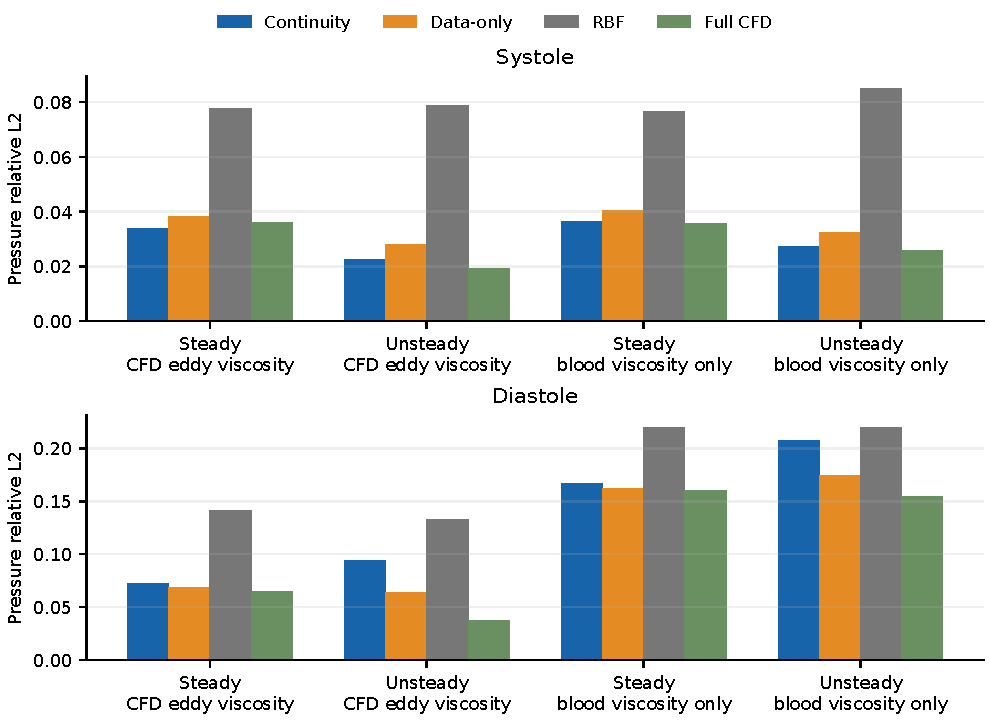
\includegraphics[width=\textwidth]{pressure_information.pdf}
\caption{Median pressure error over Cases~2--8 at 2.5~mm for the four post-processing settings. Unsteady retains the two-snapshot time derivative and steady omits it. ``\CFD eddy viscosity'' uses $\mu+\mu_t$ from the reference simulation, and ``blood viscosity only'' sets $\mu_t=0$. Full \CFD applies the same settings to the complete velocity.}
\label{fig:pressure_information}
\end{figure}

\subsection{Robustness to the choice of interpolation comparator}
\label{sec:robustness}
The prespecified \RBF used one fixed local interpolant in each snapshot. To test how much the comparison depended on that choice, we also evaluated a tuned spatial \RBF and a space-time \RBF, with their settings chosen from the withheld velocity observations. Table~\ref{tab:robustness} reports the completed comparisons for draw 0 at 2.5~mm; these values use one draw per case, so they should be compared within this table rather than directly with the three-draw means of the primary analysis.

At systole, fitting both snapshots with a space-time \RBF changed the median pressure error only slightly, from 0.079 for the prespecified \RBF to 0.074, and the \WSS error from 0.606 to 0.595. The continuity field gave errors of 0.025 and 0.356, respectively, and had lower velocity, pressure and \WSS errors than each \RBF variant in all seven cases. Tuning the spatial \RBF did not improve this phase, since its median pressure and \WSS errors were 0.127 and 0.686; therefore, choosing an interpolant by its velocity error in withheld observations did not ensure lower errors in hidden fields derived from its spatial gradients.

At diastole, both alternatives helped the interpolation. Relative to the prespecified \RBF, the tuned spatial \RBF reduced the median velocity error from 0.129 to 0.100, the pressure error from 0.136 to 0.111 and the \WSS error from 0.371 to 0.321, and the space-time \RBF reduced them to 0.096, 0.113 and 0.301. The continuity field kept lower velocity and \WSS errors than both variants in all seven cases, with a median pressure error of 0.076, but its pressure advantage held in only five of the seven diastolic cases against each variant. Over all 14 case--phase units, the continuity field had the lower pressure error in 12 against the tuned \RBF and in 12 against the space-time \RBF, with median error ratios of 0.50 and 0.54, and the lower \WSS error in all 14 against both, with median ratios of 0.54 and 0.58. It also had a lower pressure error than the better of the two variants in 12 of the 14 units. The advantage persists against the two additional interpolants tested, although they narrow the diastolic pressure gap. This does not exclude other interpolation schemes from performing better.

% Generated by generate_robustness_table.py.
\begin{table}[htbp]
\centering
\small
\caption{\revision{\textcolor{red}{Robustness to the interpolation comparator, given as median relative errors over the seven cases in each phase (Cases~2--8) with draw 0 at 2.5~mm. The tuned RBF chooses kernel, neighbourhood and smoothing on the withheld observations, while the space-time RBF interpolates both snapshots jointly with a time scale chosen the same way. All methods share the post-processing, and pressure uses the unsteady form with oracle $\mu_t$.}}}
\label{tab:robustness}
\begin{tabular}{llccc}
\toprule
Phase & Method & Velocity & Pressure & WSS \\
\midrule
Systole & Continuity field & 0.043 & 0.025 & 0.356 \\
Systole & RBF (prespecified) & 0.144 & 0.079 & 0.606 \\
Systole & RBF (tuned) & 0.177 & 0.127 & 0.686 \\
Systole & RBF (space-time) & 0.147 & 0.074 & 0.595 \\
Diastole & Continuity field & 0.038 & 0.076 & 0.173 \\
Diastole & RBF (prespecified) & 0.129 & 0.136 & 0.371 \\
Diastole & RBF (tuned) & 0.100 & 0.111 & 0.321 \\
Diastole & RBF (space-time) & 0.096 & 0.113 & 0.301 \\
\bottomrule
\end{tabular}
\end{table}



\subsection{Sensitivity to near-wall observations}
\label{sec:nearwall}
Because the grid observations are snapped to mesh nodes, some lie on the near-wall prism layers (Section~\ref{sec:observations}). To measure how much the results depend on them, we repeated draw 0 at 2.5~mm for the continuity field and \RBF after removing every observation closer than $\Delta/2=1.25$~mm to the wall, which removed 28--32\% of the observations in each case (Table~\ref{tab:nearwall}). Nothing else was changed.

The \WSS errors rose sharply. For the continuity field the median rose from 0.356 to 0.806 at systole and from 0.173 to 0.521 at diastole, and for \RBF from 0.606 to 0.886 and from 0.371 to 0.681. The accuracy of the one-sided \WSS estimate therefore rests largely on velocity sampled within about a millimetre of the wall, which a 2.5~mm imaging voxel would not resolve. Pressure was much less sensitive. The continuity field's median pressure error changed from 0.025 to 0.027 at systole and from 0.076 to 0.045 at diastole, consistent with pressure being integrated only on nodes more than 1~mm from the wall. The continuity field still had lower velocity, pressure and \WSS errors than \RBF in all 14 units, so the comparison between the methods does not depend on the near-wall samples, whereas the absolute \WSS accuracy does.

% Generated by scripts/manuscript/generate_nearwall_table.py.
\begin{table}[htbp]
\centering
\small
\caption{Sensitivity to near-wall observations. Median relative errors over Cases~2--8 for draw 0 at $\Delta=2.5$~mm, with all observations and with the observations closer than $\Delta/2=1.25$~mm to the wall removed (28--32\% of them). Pressure uses the unsteady form with CFD eddy viscosity; WSS uses $h=0.25$~mm. Velocity is scored on all unobserved nodes, so the second pair of rows is also scored on the removed nodes.}
\label{tab:nearwall}
\begin{tabular}{llccc}
\toprule
Phase & Method and observations & Velocity & Pressure & WSS \\
\midrule
Systole & Continuity field, all observations & 0.043 & 0.025 & 0.356 \\
Systole & RBF, all observations & 0.144 & 0.079 & 0.606 \\
Systole & Continuity field, none within 1.25~mm & 0.130 & 0.027 & 0.806 \\
Systole & RBF, none within 1.25~mm & 0.248 & 0.121 & 0.886 \\
\addlinespace
Diastole & Continuity field, all observations & 0.038 & 0.076 & 0.173 \\
Diastole & RBF, all observations & 0.129 & 0.136 & 0.371 \\
Diastole & Continuity field, none within 1.25~mm & 0.123 & 0.045 & 0.521 \\
Diastole & RBF, none within 1.25~mm & 0.258 & 0.108 & 0.681 \\
\bottomrule
\end{tabular}
\end{table}



\section{Discussion}
\label{sec:discussion}
\subsection{Effects of inlet diameter and asymmetry}
With the flow waveform and the maximum sac diameter held fixed, inlet diameter set the strength of the systolic disturbance and asymmetry set its location. A narrower parent vessel raised the peak Reynolds number, the jet speed entering the sac, the pressure drop, the fraction of reversed flow and the modeled eddy viscosity, and it strengthened the high-shear rings at the necks. This agrees with reports that a larger parent vessel lowers \WSS in intracranial aneurysms~\cite{fattahi2023influence}, and it extends the comparison to transitional flow in a curved, tapered thoracic segment. Because the same flow rate was prescribed for all diameters, the diameter effect here combines the change in geometry with the change in mean velocity. A study that scaled the flow rate with the vessel area would separate these two influences.

Asymmetry moved the low-shear region and the dominant vortex to the side of the larger bulge while changing the systolic pressure drop by less than 7\%. At diastole its effect became larger than that of diameter, with the asymmetric sacs carrying about two to three times the \WSS of the axisymmetric ones. A previous study of idealized abdominal and descending thoracic aneurysms also found that asymmetry mainly redistributes recirculation and \WSS~\cite{rehman2024comparative}. The present results add that the redistribution depends on the phase of the cycle, so single-instant comparisons at peak systole understate it. None of these comparisons is a population statistic, since each geometry is a single designed case, and whether low or high \WSS relates to growth or rupture cannot be settled by simulations of this kind~\cite{geers2017wall,lipp2020computational}.

\subsection{Why the neural field outperformed interpolation}
The clearest gain came from the reconstructed velocity rather than from adding momentum to the training loss. The neural fields and the prespecified \RBF received the same velocity observations and boundary values, and their pressure and \WSS were computed by the same post-processing. Yet the data field, which has no interior PDE penalty, performed close to the continuity field at 1.5 and 2.5~mm. Both neural fields also retained near-wall gradients that the prespecified \RBF tended to smooth out, and their finite-distance shear estimates recovered about 90--100\% of the \CFD 99th-percentile \WSS, compared with about half for \RBF at systole. The continuity penalty became consistently useful at the sparsest spacing, 4.0~mm.

The network fits one function across the domain and both snapshots, whereas the prespecified \RBF uses a local neighborhood at each time. This difference offers a plausible explanation for the results, but the study does not isolate the effects of spatial smoothness, joint temporal fitting and the network architecture. The space-time \RBF check narrows that interpretation, because fitting both snapshots jointly did not close the gap to the neural field at systole. At diastole, both tuning and joint temporal fitting improved all three median errors of the interpolant and reduced the continuity field's pressure advantage to five of seven cases for draw 0. These checks support the use of a neural representation in this setting without establishing that it is preferable to every interpolation scheme. Related work has used implicit neural representations for 4D flow reconstruction without a physics loss~\cite{saitta2024implicit}; here, the representation supplies velocity to the established momentum-integration route for relative pressure~\cite{krittian2012finite,bertoglio2018relative}.

The momentum \PINNs did not meet the criterion of the development test. Their poor pressure outputs, despite small momentum residuals, are consistent with a weakly determined trade-off between pressure and local acceleration. Two velocity snapshots constrain a finite difference, but they do not uniquely determine the network's time derivative between them. The diagnostic in Section~\ref{sec:pilot_results} showed that a small residual could coexist with an inaccurate pressure field. This fits the broader sensitivity of \PINNs to loss weighting and the information available to each residual~\cite{krishnapriyan2021failure,wang2021gradient}. Recovering pressure after fitting avoids relying on that pressure head, although the two-snapshot acceleration still carries reconstruction error. Longer time series, hard constraints and other loss weights might change the comparison. They were not tested here, so the negative result applies to the specified formulation and windows rather than to momentum \PINNs in general~\cite{mcgreivy2024weak}.

\subsection{Information needed for each hidden field}
Pressure and \WSS expose different weaknesses in the reconstruction of the sparse velocity. For the seven confirmation geometries, the retention of local acceleration brought the median systolic pressure error close to the complete-\CFD post-processing reference. Removing eddy viscosity did little to change that median, although the reference study of all-cases showed greater sensitivity in narrower geometries of 2.0~cm. The limited systolic sensitivity of the median should therefore not be read as evidence that eddy viscosity can always be neglected.

At diastole, omitting the \CFD eddy viscosity raised even the complete-velocity pressure error to 9--19\%. The reconstruction results with that field supplied describe a conditional calculation, because the sparse velocity observations do not themselves provide the closure. Small absolute pressure errors also matter more in this phase. None of the tested methods reliably recovered the diastolic pressure drop, even when its relative error across the field appeared modest. An estimate of eddy viscosity and a better-resolved acceleration are, therefore, separate requirements to examine before applying this calculation to measured data.

For aneurysm-zone \WSS, near-wall sampling remained the main limitation. Removing the observations within 1.25~mm of the wall more than doubled the continuity field's \WSS error at both phases while leaving the ranking against \RBF unchanged (Section~\ref{sec:nearwall}). The error depended on the distance used by the one-sided estimate, and the reconstructed fields remained above the complete-\CFD reference. Outside the aneurysm zone, the interior node closest to the wall was a median of 0.58~mm from it; even the complete \CFD velocity then gave a poor estimate of the exported shear. This is consistent with the documented sensitivity of velocity-derived \WSS to spatial resolution~\cite{petersson2012assessment,stalder2008quantitative}. A smooth velocity fit and an analytic derivative do not, by themselves, establish an accurate wall gradient.

\subsection{Limitations}
\label{Limitations}
The twelve geometries form a designed family, not a patient cohort. They share one maximum aneurysm diameter, taper ratio and inflow waveform, and they contain no branches. The seven confirmation geometries therefore test variation within that family. The rigid-wall flow solution has reported mesh, time-step and cycle checks for aneurysm \WSS, but no experimental validation. The structural calculation uses a uniform 2~mm wall, literature material parameters, fixed ends and a quasi-static coupling. Its coupling-step and mesh-update settings were not retained with the results, and no solid-mesh convergence check is available, so the stress fields are used only to describe modeled stress concentrations.

The temporal records also have limits. Each reconstruction uses two snapshots from a short window. Several instants were retained, but no complete cycle-resolved wall-traction series is available. The solver exported \TAWSS to the wall nodes, but its cycle-resolved components did not, so the oscillatory indices were not evaluated. The slice workbook does not state its averaging interval; the slice values were identified as cycle averages from the inlet flow rate.

The observed velocities are noise-free \CFD values at the mesh nodes. They do not include partial-volume averaging, noise, segmentation error, or velocity aliasing of 4D flow MRI~\cite{markl2012fourd}, and some lie within a fraction of a millimeter of the wall (Section~\ref{sec:observations}). Without observations within 1.25~mm of the wall, the \WSS errors were more than twice as large (Section~\ref{sec:nearwall}), so the absolute \WSS precision reported here should not be expected from the imaging data. Performance on measured data may therefore be worse. Pressure calculations with \CFD-supplied eddy viscosity additionally assume closure information that would have to be estimated in practice. The errors are node-weighted because the exports contain no cell volumes, which gives a greater weight to the refined near-wall mesh.

The network architecture and training settings were fixed on the development cases without a wider hyperparameter search. The tuned and space-time \RBF checks were added after the primary verdict and use one draw per case; they cannot replace the three-draw comparison. A divergence-free interpolant, the natural non-neural counterpart of the continuity field, was not tested. Every method receives observations in the target geometry. The prediction in a geometry with no observations was not tested. Finally, fitting a neural field took about 20~min on a GPU per window, so its accuracy came at a higher computational cost than interpolation.

\section{Conclusion}
\label{sec:conclusion}
Twelve idealized descending thoracic aortic geometries, comprising nine aneurysmal models with a fixed maximum sac diameter of 4.0~cm and three nonaneurysmal controls, were simulated with transient transitional \CFD, and their common-time fields were used both to compare the geometries and to test the recovery of hidden pressure and \WSS from sparse velocity. The inlet diameter dominated the systolic response. Reducing it from 2.6 to 2.0~cm raised the pressure drop 2.3--2.5 times, roughly doubled the fraction of reversed flow in dilation, and raised the 95th-percentile \WSS in the necks from 7--8 to 15--18~Pa, while the bulge pattern changed the drop in systolic pressure by less than 7\%. Instead, asymmetry relocated the low-shear region and the dominant vortex to the larger bulge, and at diastole it raised the median \WSS of the dilation segment 1.8--3.1 times relative to the axisymmetric sacs.

With velocity observed at about 1.3\% of the interior nodes at two instants, a continuity-constrained space-time neural field followed by momentum integration and a near-wall shear estimate recovered pressure and aneurysm-zone \WSS more accurately than the same post-processing applied to the prespecified \RBF in all 14 confirmation units after averaging three draws per unit, with median error ratios of 0.46 and 0.51. The pressure advantage was small at diastole. The benefit came mainly from the neural representation of the velocity. A continuity penalty helped in the sparsest sampling, and momentum \PINNs did not meet the development-test criterion for joint pressure and shear recovery. Systolic pressure was recovered close to the accuracy of post-processing itself, diastolic pressure errors increased when the \CFD-supplied eddy viscosity was omitted, and \WSS accuracy depended on the velocity sampled close to the wall, although the continuity field retained its advantage over \RBF without those samples. These findings identify what information each hidden field needs in this idealized, noise-free setting. Measured velocity data, estimated closures, and patient-specific anatomies are the next tests, and none of the results constitutes a clinical rupture-risk assessment.

\section*{Declarations}
\paragraph{Conflicts of interest.} The authors have no conflicts to disclose.

\ifanonymized
\paragraph{Funding and author contributions.} Removed for anonymized review.
\else
\paragraph{Funding.} Helmi Temimi thanks the Kuwait Foundation for the Advancement of Sciences (Project Code: CN22-16QE-1643).

\paragraph{Author contributions.} Conceptualization, M.A.U.R. and M.A.O.; \CFD and structural modeling, M.A.U.R.; reconstruction methodology, software and formal analysis of the reconstruction study, M.A.O.; validation, M.A.U.R., M.A.O., F.J. and H.T.; data curation, M.A.U.R. and M.A.O.; writing (original draft), M.A.U.R. and M.A.O.; writing (review and editing), all authors; funding acquisition, F.J. and H.T. All authors have read and agreed to the submitted version.
\fi


% AUTHOR CHECK: the existing AI-use declaration remains commented. Apply the target journal's policy and describe actual use accurately.
% \paragraph{Use of generative AI.} During the preparation of this work, the authors used Claude (Anthropic) and Codex (OpenAI) to help write and edit the language and grammar of the manuscript. The simulations, the study design and the interpretation of the results are the authors' own. The authors reviewed and edited all AI-assisted output and take full responsibility for the content of the publication.

\paragraph{Data availability statement.} The \CFD exports analyzed in this study are available from the corresponding author on reasonable request. \ifanonymized The reconstruction code and configuration files are available in a public repository whose link is withheld for anonymized review.\else The reconstruction code and configuration files are available at \url{https://github.com/michaelajao/IdealAorta-PINN}.\fi

\appendix
\section{Case-wise reconstruction results}
\label{app:casewise}
Tables~\ref{tab:case_pressure} and \ref{tab:case_shear} list every confirmation unit at 2.5~mm, spread over the three paired draws and the range of draw-wise error ratios to \RBF.

\begin{table}[htbp]
\centering
\small
\caption{Case-wise pressure relative L2 at 2.5~mm, given as the mean (sample standard deviation) over three paired observation/initialization draws. The last column is the range of draw-wise continuity/RBF error ratios, and values above one favor RBF. The spread describes these draws, not patient-population uncertainty.}
\label{tab:case_pressure}
\begin{tabular}{llcccc}
\toprule
Case & Phase & Continuity & Data-only & RBF & Ratio range \\
\midrule
2 & Sys. & 0.069 (0.004) & 0.069 (0.008) & 0.111 (0.010) & 0.53--0.68 \\
2 & Dia. & 0.094 (0.026) & 0.050 (0.012) & 0.138 (0.016) & 0.55--0.81 \\
3 & Sys. & 0.031 (0.004) & 0.030 (0.004) & 0.078 (0.009) & 0.35--0.47 \\
3 & Dia. & 0.028 (0.004) & 0.032 (0.003) & 0.095 (0.014) & 0.27--0.32 \\
4 & Sys. & 0.023 (0.001) & 0.027 (0.008) & 0.093 (0.019) & 0.20--0.30 \\
4 & Dia. & 0.107 (0.032) & 0.071 (0.020) & 0.157 (0.018) & 0.50--1.05 \\
5 & Sys. & 0.022 (0.002) & 0.028 (0.002) & 0.079 (0.011) & 0.24--0.31 \\
5 & Dia. & 0.044 (0.017) & 0.059 (0.027) & 0.113 (0.015) & 0.29--0.56 \\
6 & Sys. & 0.020 (0.000) & 0.027 (0.004) & 0.081 (0.017) & 0.20--0.30 \\
6 & Dia. & 0.085 (0.029) & 0.093 (0.031) & 0.132 (0.004) & 0.51--0.89 \\
7 & Sys. & 0.021 (0.004) & 0.022 (0.003) & 0.074 (0.015) & 0.25--0.34 \\
7 & Dia. & 0.155 (0.085) & 0.090 (0.035) & 0.171 (0.008) & 0.54--1.40 \\
8 & Sys. & 0.032 (0.005) & 0.030 (0.009) & 0.063 (0.007) & 0.50--0.54 \\
8 & Dia. & 0.101 (0.076) & 0.063 (0.011) & 0.104 (0.005) & 0.31--1.75 \\
\bottomrule
\end{tabular}
\end{table}

\begin{table}[htbp]
\centering
\small
\caption{Case-wise wall-shear magnitude relative L2 at 2.5~mm, given as the mean (sample standard deviation) over three paired observation/initialization draws. The last column is the range of draw-wise continuity/RBF error ratios, and values above one favor RBF. The spread describes these draws, not patient-population uncertainty.}
\label{tab:case_shear}
\begin{tabular}{llcccc}
\toprule
Case & Phase & Continuity & Data-only & RBF & Ratio range \\
\midrule
2 & Sys. & 0.417 (0.007) & 0.386 (0.018) & 0.653 (0.004) & 0.63--0.65 \\
2 & Dia. & 0.166 (0.009) & 0.169 (0.029) & 0.404 (0.002) & 0.39--0.43 \\
3 & Sys. & 0.363 (0.010) & 0.333 (0.026) & 0.636 (0.008) & 0.55--0.60 \\
3 & Dia. & 0.166 (0.006) & 0.148 (0.013) & 0.409 (0.005) & 0.39--0.43 \\
4 & Sys. & 0.329 (0.033) & 0.306 (0.018) & 0.605 (0.001) & 0.51--0.61 \\
4 & Dia. & 0.131 (0.004) & 0.150 (0.020) & 0.302 (0.002) & 0.42--0.44 \\
5 & Sys. & 0.356 (0.005) & 0.359 (0.011) & 0.619 (0.010) & 0.56--0.59 \\
5 & Dia. & 0.163 (0.018) & 0.174 (0.008) & 0.386 (0.001) & 0.37--0.45 \\
6 & Sys. & 0.373 (0.002) & 0.352 (0.027) & 0.609 (0.005) & 0.61--0.62 \\
6 & Dia. & 0.155 (0.030) & 0.161 (0.008) & 0.368 (0.003) & 0.33--0.50 \\
7 & Sys. & 0.323 (0.012) & 0.300 (0.011) & 0.590 (0.005) & 0.53--0.57 \\
7 & Dia. & 0.136 (0.004) & 0.146 (0.019) & 0.332 (0.005) & 0.40--0.43 \\
8 & Sys. & 0.330 (0.012) & 0.327 (0.009) & 0.598 (0.005) & 0.54--0.58 \\
8 & Dia. & 0.176 (0.022) & 0.196 (0.013) & 0.374 (0.005) & 0.40--0.51 \\
\bottomrule
\end{tabular}
\end{table}


\newpage
\bibliographystyle{unsrt}
\bibliography{bib/tsb,bib/references}

\end{document}
